% -*- program: xelatex -*-

\documentclass[
	12pt
	]{beamer}

% -----------------------------------------------------------------------------
% theming
\usetheme[numbering=fraction,
	progressbar=frametitle,
	% background=dark
	]{metropolis}


% % use a heavier font for large room/underpowered projector
% \setsansfont[BoldFont={Fira Sans SemiBold}]{Fira Sans Book}

% % can use every beamer color theme!
% \usecolortheme{crane}
% \useoutertheme{metropolis}
% \useinnertheme{metropolis}
% \usefonttheme{metropolis}

% % or set colors by hand
\definecolor{myblue}{rgb}{0.047, 0.298, 0.435}
\definecolor{myalert}{rgb}{0.847, 0.510, 0.106}

% change header color
\setbeamercolor{frametitle}{bg=myblue}
% \setbeamercolor{...}{fg=...,bg=...}
% \setbeamercolor{progress bar}{...}
% \setbeamercolor{title separator}{...}
% \setbeamercolor{progress bar in head/foot}{...}
% \setbeamercolor{progress bar in section page}{...}

% slightly darker organce
\setbeamercolor{alerted text}{fg=myalert}



% change width of title separator, section page separator % progress
%https://github.com/matze/mtheme/issues/237
\makeatletter
\setlength{\metropolis@titleseparator@linewidth}{1pt}
\setlength{\metropolis@progressonsectionpage@linewidth}{2pt}
\setlength{\metropolis@progressinheadfoot@linewidth}{2pt}
\makeatother


% environment for alerts (=colored bullet)
% http://tex.stackexchange.com/questions/14319/beamer-change-individual-bullet-color-in-itemize-list
\newenvironment{aleenv}{\only{\setbeamercolor{local structure}{fg=myalert}}}{}

% Put graphic anywhere on slide using Put(x, y){}
% with x, y in pt
% http://tex.stackexchange.com/questions/34921/how-to-overlap-images-in-a-beamer-slide
\def\Put(#1,#2)#3{\leavevmode\makebox(0,0){\put(#1,#2){#3}}}


% -----------------------------------------------------------------------------
% do not count appendix slides, use \appendix to indicate 
\usepackage{appendixnumberbeamer}  
% creative commons icons
\usepackage[scale=2
	]{ccicons} 
% fontawesome font/icons
\usepackage{fontspec}
\usepackage{fontawesome}      %
\usepackage{pifont}

% Graphics
\usepackage{graphicx}
\usepackage{tikz}
\usetikzlibrary{shapes, arrows, positioning, calc, arrows.meta, snakes}
\usepackage{adjustbox}


% use speaker notes
\usepackage{pgfpages}
\setbeameroption{hide notes} % Only slides
%\setbeameroption{show only notes} % Only notes
% \setbeameroption{show notes on second screen=right} % Both




% for overview.tikz figure
\newlength\yearposx


%%% ---------------------------------------------------------------------------
\title{Statistical Eco(-toxico)logy}
\subtitle{Improving the Utilisation of Data for\\Environmental Risk Assessment}
\date{25\textsuperscript{th} January 2017}
\author{Eduard Sz\"{o}cs}



%%% ---------------------------------------------------------------------------
\begin{document}

%%% ------------------------------
\maketitle

\begin{frame}{Table of contents}
  \setbeamertemplate{section in toc}[sections numbered]
  \tableofcontents[hideallsubsections]
\end{frame}


%%% ---------------------------------------------------------------------------
{%
\setbeamertemplate{frame footer}{WWF (2016), Living Planet Report; Vörösmarty (2010). Nature.
}
\begin{frame}[t]
\frametitle{Freshwater biodiversity is strongly declining}
	\begin{columns}[T]
	\column{.63\textwidth}
		\onslide<1->{
			% \resizebox{1.1\textwidth}{!}{%
			% 			\hspace{-5mm}% Created by tikzDevice version 0.10.1 on 2017-01-20 09:42:50
% !TEX encoding = UTF-8 Unicode
\begin{tikzpicture}[x=1pt,y=1pt]
\definecolor{fillColor}{RGB}{255,255,255}
\path[use as bounding box,fill=fillColor,fill opacity=0.00] (0,0) rectangle (505.89,405.01);
\begin{scope}
\path[clip] (  0.00,  0.00) rectangle (505.89,405.01);
\definecolor{drawColor}{RGB}{255,255,255}
\definecolor{fillColor}{RGB}{255,255,255}

\path[draw=drawColor,line width= 0.6pt,line join=round,line cap=round,fill=fillColor] (  0.00,  0.00) rectangle (505.89,405.01);
\end{scope}
\begin{scope}
\path[clip] ( 58.39, 81.11) rectangle (498.89,376.10);
\definecolor{fillColor}{RGB}{255,255,255}

\path[fill=fillColor] ( 58.39, 81.11) rectangle (498.89,376.10);
\definecolor{drawColor}{RGB}{70,130,180}

\path[draw=drawColor,line width= 1.7pt,line join=round] ( 80.80,274.77) --
	( 86.76,266.71) --
	( 96.30,264.51) --
	(106.43,265.24) --
	(122.52,257.91) --
	(137.41,246.92) --
	(154.69,242.53) --
	(175.55,235.93) --
	(191.04,227.14) --
	(201.77,222.74) --
	(211.90,211.02) --
	(226.20,206.63) --
	(238.72,194.90) --
	(248.85,178.05) --
	(269.70,174.39) --
	(277.45,167.06) --
	(292.94,165.59) --
	(307.25,159.00) --
	(316.78,159.00) --
	(337.64,151.67) --
	(358.49,142.88) --
	(385.91,135.55) --
	(403.78,135.55) --
	(416.89,130.42) --
	(431.19,128.96) --
	(444.90,135.55) --
	(452.05,140.68) --
	(468.14,131.89) --
	(478.87,128.23);
\definecolor{drawColor}{RGB}{0,0,139}

\path[draw=drawColor,line width= 1.7pt,line join=round] ( 78.42,274.03) --
	( 95.08,263.81) --
	(109.95,266.73) --
	(126.61,269.65) --
	(144.46,266.00) --
	(153.98,260.90) --
	(164.09,260.17) --
	(179.56,251.41) --
	(196.82,245.57) --
	(208.72,239.00) --
	(221.81,229.52) --
	(235.49,220.03) --
	(249.77,211.28) --
	(272.97,214.19) --
	(301.53,210.55) --
	(330.69,207.63) --
	(357.46,207.63) --
	(389.00,208.36) --
	(419.93,209.09) --
	(430.64,212.74) --
	(449.09,209.09) --
	(467.53,210.55) --
	(477.65,210.55);
\definecolor{drawColor}{RGB}{0,139,0}

\path[draw=drawColor,line width= 1.7pt,line join=round] ( 80.83,275.43) --
	(103.50,267.98) --
	(130.37,265.85) --
	(153.89,250.95) --
	(162.28,248.83) --
	(172.36,253.08) --
	(183.28,252.02) --
	(210.15,245.63) --
	(246.26,245.63) --
	(279.85,240.31) --
	(324.36,228.61) --
	(344.51,230.73) --
	(362.14,220.09) --
	(373.90,221.16) --
	(383.98,217.96) --
	(412.53,217.96) --
	(421.77,224.35) --
	(441.08,212.64) --
	(452.00,215.84) --
	(478.87,206.26);
\definecolor{drawColor}{RGB}{0,0,0}

\path[draw=drawColor,line width= 0.6pt,dash pattern=on 1pt off 3pt ,line join=round] ( 58.39,273.30) -- (498.89,273.30);
\definecolor{drawColor}{gray}{0.50}

\path[draw=drawColor,line width= 0.6pt,line join=round,line cap=round] ( 58.39, 81.11) rectangle (498.89,376.10);
\end{scope}
\begin{scope}
\path[clip] (  0.00,  0.00) rectangle (505.89,405.01);
\definecolor{drawColor}{gray}{0.30}

\node[text=drawColor,anchor=base east,inner sep=0pt, outer sep=0pt, scale=  1.54] at ( 52.09, 83.90) {\bfseries 0.0};

\node[text=drawColor,anchor=base east,inner sep=0pt, outer sep=0pt, scale=  1.54] at ( 52.09,173.28) {\bfseries 0.5};

\node[text=drawColor,anchor=base east,inner sep=0pt, outer sep=0pt, scale=  1.54] at ( 52.09,262.67) {\bfseries 1.0};

\node[text=drawColor,anchor=base east,inner sep=0pt, outer sep=0pt, scale=  1.54] at ( 52.09,352.06) {\bfseries 1.5};
\end{scope}
\begin{scope}
\path[clip] (  0.00,  0.00) rectangle (505.89,405.01);
\definecolor{drawColor}{RGB}{0,0,0}

\path[draw=drawColor,line width= 0.6pt,line join=round] ( 54.89, 94.52) --
	( 58.39, 94.52);

\path[draw=drawColor,line width= 0.6pt,line join=round] ( 54.89,183.91) --
	( 58.39,183.91);

\path[draw=drawColor,line width= 0.6pt,line join=round] ( 54.89,273.30) --
	( 58.39,273.30);

\path[draw=drawColor,line width= 0.6pt,line join=round] ( 54.89,362.69) --
	( 58.39,362.69);
\end{scope}
\begin{scope}
\path[clip] (  0.00,  0.00) rectangle (505.89,405.01);
\definecolor{drawColor}{RGB}{0,0,0}

\path[draw=drawColor,line width= 0.6pt,line join=round] ( 76.63, 77.61) --
	( 76.63, 81.11);

\path[draw=drawColor,line width= 0.6pt,line join=round] (172.57, 77.61) --
	(172.57, 81.11);

\path[draw=drawColor,line width= 0.6pt,line join=round] (268.51, 77.61) --
	(268.51, 81.11);

\path[draw=drawColor,line width= 0.6pt,line join=round] (364.45, 77.61) --
	(364.45, 81.11);

\path[draw=drawColor,line width= 0.6pt,line join=round] (460.39, 77.61) --
	(460.39, 81.11);
\end{scope}
\begin{scope}
\path[clip] (  0.00,  0.00) rectangle (505.89,405.01);
\definecolor{drawColor}{gray}{0.30}

\node[text=drawColor,anchor=base,inner sep=0pt, outer sep=0pt, scale=  1.54] at ( 76.63, 64.19) {\bfseries 1970};

\node[text=drawColor,anchor=base,inner sep=0pt, outer sep=0pt, scale=  1.54] at (172.57, 64.19) {\bfseries 1980};

\node[text=drawColor,anchor=base,inner sep=0pt, outer sep=0pt, scale=  1.54] at (268.51, 64.19) {\bfseries 1990};

\node[text=drawColor,anchor=base,inner sep=0pt, outer sep=0pt, scale=  1.54] at (364.45, 64.19) {\bfseries 2000};

\node[text=drawColor,anchor=base,inner sep=0pt, outer sep=0pt, scale=  1.54] at (460.39, 64.19) {\bfseries 2010};
\end{scope}
\begin{scope}
\path[clip] (  0.00,  0.00) rectangle (505.89,405.01);
\definecolor{drawColor}{RGB}{0,0,0}

\node[text=drawColor,anchor=base,inner sep=0pt, outer sep=0pt, scale=  1.68] at (278.64, 47.02) {Year};
\end{scope}
\begin{scope}
\path[clip] (  0.00,  0.00) rectangle (505.89,405.01);
\definecolor{drawColor}{RGB}{0,0,0}

\node[text=drawColor,rotate= 90.00,anchor=base,inner sep=0pt, outer sep=0pt, scale=  1.68] at ( 22.62,228.61) {Index value (1970 = 1)};
\end{scope}
\begin{scope}
\path[clip] (  0.00,  0.00) rectangle (505.89,405.01);
\definecolor{fillColor}{RGB}{255,255,255}

\path[fill=fillColor] (157.35,  7.00) rectangle (399.93, 32.84);
\end{scope}
\begin{scope}
\path[clip] (  0.00,  0.00) rectangle (505.89,405.01);
\definecolor{drawColor}{RGB}{0,0,0}

\node[text=drawColor,anchor=base west,inner sep=0pt, outer sep=0pt, scale=  1.40] at (163.04, 15.10) {Habitat};
\end{scope}
\begin{scope}
\path[clip] (  0.00,  0.00) rectangle (505.89,405.01);
\definecolor{drawColor}{RGB}{0,139,0}

\path[draw=drawColor,line width= 4.6pt,line join=round] (215.15, 19.92) -- (226.71, 19.92);
\end{scope}
\begin{scope}
\path[clip] (  0.00,  0.00) rectangle (505.89,405.01);
\definecolor{drawColor}{RGB}{0,0,139}

\path[draw=drawColor,line width= 4.6pt,line join=round] (277.53, 19.92) -- (289.10, 19.92);
\end{scope}
\begin{scope}
\path[clip] (  0.00,  0.00) rectangle (505.89,405.01);
\definecolor{drawColor}{RGB}{70,130,180}

\path[draw=drawColor,line width= 4.6pt,line join=round] (329.23, 19.92) -- (340.79, 19.92);
\end{scope}
\begin{scope}
\path[clip] (  0.00,  0.00) rectangle (505.89,405.01);
\definecolor{drawColor}{RGB}{0,0,0}

\node[text=drawColor,anchor=base west,inner sep=0pt, outer sep=0pt, scale=  1.12] at (229.96, 16.06) {terrestric};
\end{scope}
\begin{scope}
\path[clip] (  0.00,  0.00) rectangle (505.89,405.01);
\definecolor{drawColor}{RGB}{0,0,0}

\node[text=drawColor,anchor=base west,inner sep=0pt, outer sep=0pt, scale=  1.12] at (292.35, 16.06) {marine};
\end{scope}
\begin{scope}
\path[clip] (  0.00,  0.00) rectangle (505.89,405.01);
\definecolor{drawColor}{RGB}{0,0,0}

\node[text=drawColor,anchor=base west,inner sep=0pt, outer sep=0pt, scale=  1.12] at (344.04, 16.06) {freshwater};
\end{scope}
\begin{scope}
\path[clip] (  0.00,  0.00) rectangle (505.89,405.01);
\definecolor{drawColor}{RGB}{0,0,0}

\node[text=drawColor,anchor=base west,inner sep=0pt, outer sep=0pt, scale=  1.68] at ( 58.39,386.44) {Living Planet Index};
\end{scope}
\end{tikzpicture}

			% 			}

			% \hspace{-7mm}\begin{adjustbox}{max totalsize={1.1\textwidth}{\textheight}}
			% 	% Created by tikzDevice version 0.10.1 on 2017-01-20 09:42:50
% !TEX encoding = UTF-8 Unicode
\begin{tikzpicture}[x=1pt,y=1pt]
\definecolor{fillColor}{RGB}{255,255,255}
\path[use as bounding box,fill=fillColor,fill opacity=0.00] (0,0) rectangle (505.89,405.01);
\begin{scope}
\path[clip] (  0.00,  0.00) rectangle (505.89,405.01);
\definecolor{drawColor}{RGB}{255,255,255}
\definecolor{fillColor}{RGB}{255,255,255}

\path[draw=drawColor,line width= 0.6pt,line join=round,line cap=round,fill=fillColor] (  0.00,  0.00) rectangle (505.89,405.01);
\end{scope}
\begin{scope}
\path[clip] ( 58.39, 81.11) rectangle (498.89,376.10);
\definecolor{fillColor}{RGB}{255,255,255}

\path[fill=fillColor] ( 58.39, 81.11) rectangle (498.89,376.10);
\definecolor{drawColor}{RGB}{70,130,180}

\path[draw=drawColor,line width= 1.7pt,line join=round] ( 80.80,274.77) --
	( 86.76,266.71) --
	( 96.30,264.51) --
	(106.43,265.24) --
	(122.52,257.91) --
	(137.41,246.92) --
	(154.69,242.53) --
	(175.55,235.93) --
	(191.04,227.14) --
	(201.77,222.74) --
	(211.90,211.02) --
	(226.20,206.63) --
	(238.72,194.90) --
	(248.85,178.05) --
	(269.70,174.39) --
	(277.45,167.06) --
	(292.94,165.59) --
	(307.25,159.00) --
	(316.78,159.00) --
	(337.64,151.67) --
	(358.49,142.88) --
	(385.91,135.55) --
	(403.78,135.55) --
	(416.89,130.42) --
	(431.19,128.96) --
	(444.90,135.55) --
	(452.05,140.68) --
	(468.14,131.89) --
	(478.87,128.23);
\definecolor{drawColor}{RGB}{0,0,139}

\path[draw=drawColor,line width= 1.7pt,line join=round] ( 78.42,274.03) --
	( 95.08,263.81) --
	(109.95,266.73) --
	(126.61,269.65) --
	(144.46,266.00) --
	(153.98,260.90) --
	(164.09,260.17) --
	(179.56,251.41) --
	(196.82,245.57) --
	(208.72,239.00) --
	(221.81,229.52) --
	(235.49,220.03) --
	(249.77,211.28) --
	(272.97,214.19) --
	(301.53,210.55) --
	(330.69,207.63) --
	(357.46,207.63) --
	(389.00,208.36) --
	(419.93,209.09) --
	(430.64,212.74) --
	(449.09,209.09) --
	(467.53,210.55) --
	(477.65,210.55);
\definecolor{drawColor}{RGB}{0,139,0}

\path[draw=drawColor,line width= 1.7pt,line join=round] ( 80.83,275.43) --
	(103.50,267.98) --
	(130.37,265.85) --
	(153.89,250.95) --
	(162.28,248.83) --
	(172.36,253.08) --
	(183.28,252.02) --
	(210.15,245.63) --
	(246.26,245.63) --
	(279.85,240.31) --
	(324.36,228.61) --
	(344.51,230.73) --
	(362.14,220.09) --
	(373.90,221.16) --
	(383.98,217.96) --
	(412.53,217.96) --
	(421.77,224.35) --
	(441.08,212.64) --
	(452.00,215.84) --
	(478.87,206.26);
\definecolor{drawColor}{RGB}{0,0,0}

\path[draw=drawColor,line width= 0.6pt,dash pattern=on 1pt off 3pt ,line join=round] ( 58.39,273.30) -- (498.89,273.30);
\definecolor{drawColor}{gray}{0.50}

\path[draw=drawColor,line width= 0.6pt,line join=round,line cap=round] ( 58.39, 81.11) rectangle (498.89,376.10);
\end{scope}
\begin{scope}
\path[clip] (  0.00,  0.00) rectangle (505.89,405.01);
\definecolor{drawColor}{gray}{0.30}

\node[text=drawColor,anchor=base east,inner sep=0pt, outer sep=0pt, scale=  1.54] at ( 52.09, 83.90) {\bfseries 0.0};

\node[text=drawColor,anchor=base east,inner sep=0pt, outer sep=0pt, scale=  1.54] at ( 52.09,173.28) {\bfseries 0.5};

\node[text=drawColor,anchor=base east,inner sep=0pt, outer sep=0pt, scale=  1.54] at ( 52.09,262.67) {\bfseries 1.0};

\node[text=drawColor,anchor=base east,inner sep=0pt, outer sep=0pt, scale=  1.54] at ( 52.09,352.06) {\bfseries 1.5};
\end{scope}
\begin{scope}
\path[clip] (  0.00,  0.00) rectangle (505.89,405.01);
\definecolor{drawColor}{RGB}{0,0,0}

\path[draw=drawColor,line width= 0.6pt,line join=round] ( 54.89, 94.52) --
	( 58.39, 94.52);

\path[draw=drawColor,line width= 0.6pt,line join=round] ( 54.89,183.91) --
	( 58.39,183.91);

\path[draw=drawColor,line width= 0.6pt,line join=round] ( 54.89,273.30) --
	( 58.39,273.30);

\path[draw=drawColor,line width= 0.6pt,line join=round] ( 54.89,362.69) --
	( 58.39,362.69);
\end{scope}
\begin{scope}
\path[clip] (  0.00,  0.00) rectangle (505.89,405.01);
\definecolor{drawColor}{RGB}{0,0,0}

\path[draw=drawColor,line width= 0.6pt,line join=round] ( 76.63, 77.61) --
	( 76.63, 81.11);

\path[draw=drawColor,line width= 0.6pt,line join=round] (172.57, 77.61) --
	(172.57, 81.11);

\path[draw=drawColor,line width= 0.6pt,line join=round] (268.51, 77.61) --
	(268.51, 81.11);

\path[draw=drawColor,line width= 0.6pt,line join=round] (364.45, 77.61) --
	(364.45, 81.11);

\path[draw=drawColor,line width= 0.6pt,line join=round] (460.39, 77.61) --
	(460.39, 81.11);
\end{scope}
\begin{scope}
\path[clip] (  0.00,  0.00) rectangle (505.89,405.01);
\definecolor{drawColor}{gray}{0.30}

\node[text=drawColor,anchor=base,inner sep=0pt, outer sep=0pt, scale=  1.54] at ( 76.63, 64.19) {\bfseries 1970};

\node[text=drawColor,anchor=base,inner sep=0pt, outer sep=0pt, scale=  1.54] at (172.57, 64.19) {\bfseries 1980};

\node[text=drawColor,anchor=base,inner sep=0pt, outer sep=0pt, scale=  1.54] at (268.51, 64.19) {\bfseries 1990};

\node[text=drawColor,anchor=base,inner sep=0pt, outer sep=0pt, scale=  1.54] at (364.45, 64.19) {\bfseries 2000};

\node[text=drawColor,anchor=base,inner sep=0pt, outer sep=0pt, scale=  1.54] at (460.39, 64.19) {\bfseries 2010};
\end{scope}
\begin{scope}
\path[clip] (  0.00,  0.00) rectangle (505.89,405.01);
\definecolor{drawColor}{RGB}{0,0,0}

\node[text=drawColor,anchor=base,inner sep=0pt, outer sep=0pt, scale=  1.68] at (278.64, 47.02) {Year};
\end{scope}
\begin{scope}
\path[clip] (  0.00,  0.00) rectangle (505.89,405.01);
\definecolor{drawColor}{RGB}{0,0,0}

\node[text=drawColor,rotate= 90.00,anchor=base,inner sep=0pt, outer sep=0pt, scale=  1.68] at ( 22.62,228.61) {Index value (1970 = 1)};
\end{scope}
\begin{scope}
\path[clip] (  0.00,  0.00) rectangle (505.89,405.01);
\definecolor{fillColor}{RGB}{255,255,255}

\path[fill=fillColor] (157.35,  7.00) rectangle (399.93, 32.84);
\end{scope}
\begin{scope}
\path[clip] (  0.00,  0.00) rectangle (505.89,405.01);
\definecolor{drawColor}{RGB}{0,0,0}

\node[text=drawColor,anchor=base west,inner sep=0pt, outer sep=0pt, scale=  1.40] at (163.04, 15.10) {Habitat};
\end{scope}
\begin{scope}
\path[clip] (  0.00,  0.00) rectangle (505.89,405.01);
\definecolor{drawColor}{RGB}{0,139,0}

\path[draw=drawColor,line width= 4.6pt,line join=round] (215.15, 19.92) -- (226.71, 19.92);
\end{scope}
\begin{scope}
\path[clip] (  0.00,  0.00) rectangle (505.89,405.01);
\definecolor{drawColor}{RGB}{0,0,139}

\path[draw=drawColor,line width= 4.6pt,line join=round] (277.53, 19.92) -- (289.10, 19.92);
\end{scope}
\begin{scope}
\path[clip] (  0.00,  0.00) rectangle (505.89,405.01);
\definecolor{drawColor}{RGB}{70,130,180}

\path[draw=drawColor,line width= 4.6pt,line join=round] (329.23, 19.92) -- (340.79, 19.92);
\end{scope}
\begin{scope}
\path[clip] (  0.00,  0.00) rectangle (505.89,405.01);
\definecolor{drawColor}{RGB}{0,0,0}

\node[text=drawColor,anchor=base west,inner sep=0pt, outer sep=0pt, scale=  1.12] at (229.96, 16.06) {terrestric};
\end{scope}
\begin{scope}
\path[clip] (  0.00,  0.00) rectangle (505.89,405.01);
\definecolor{drawColor}{RGB}{0,0,0}

\node[text=drawColor,anchor=base west,inner sep=0pt, outer sep=0pt, scale=  1.12] at (292.35, 16.06) {marine};
\end{scope}
\begin{scope}
\path[clip] (  0.00,  0.00) rectangle (505.89,405.01);
\definecolor{drawColor}{RGB}{0,0,0}

\node[text=drawColor,anchor=base west,inner sep=0pt, outer sep=0pt, scale=  1.12] at (344.04, 16.06) {freshwater};
\end{scope}
\begin{scope}
\path[clip] (  0.00,  0.00) rectangle (505.89,405.01);
\definecolor{drawColor}{RGB}{0,0,0}

\node[text=drawColor,anchor=base west,inner sep=0pt, outer sep=0pt, scale=  1.68] at ( 58.39,386.44) {Living Planet Index};
\end{scope}
\end{tikzpicture}

			% \end{adjustbox}
			\hspace{-7mm}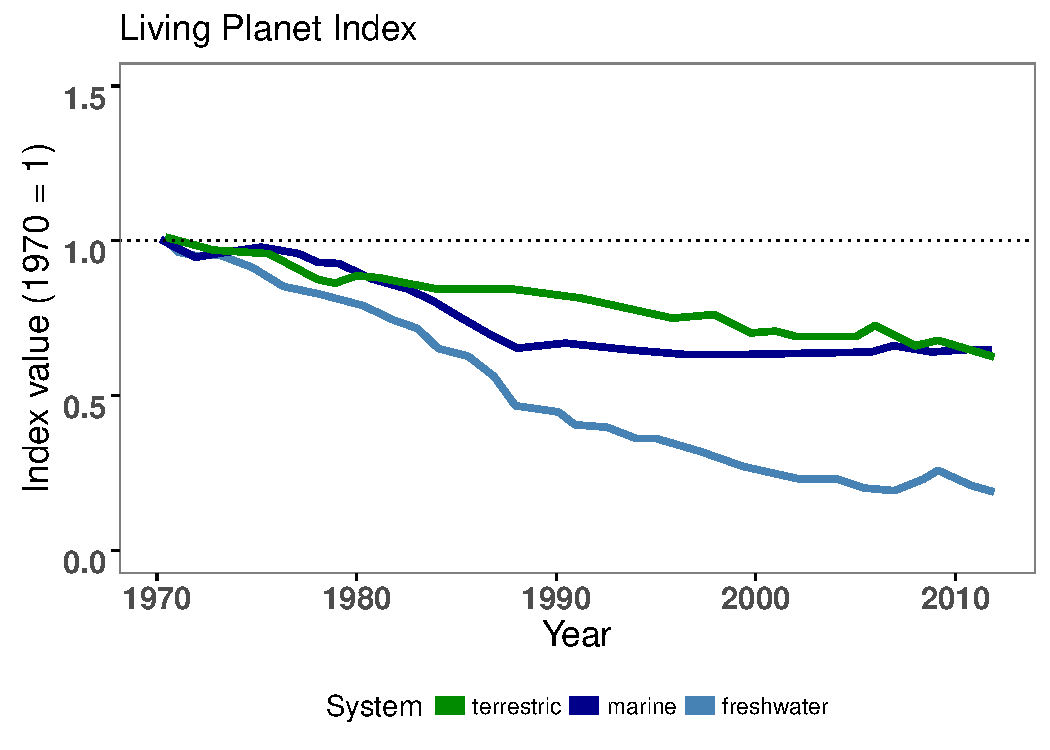
\includegraphics[width=1.1\textwidth]{figs/lpi_2016.pdf}
		}
	\column{.37\textwidth}
		\onslide<2->{
			\vspace{3em} 
			\alert{\underline{Reasons}} \\
			\begin{itemize}
				\item Habitat loss
				\item Overexploitation
				\only<-2>{\item Pollution}
				\only<3->{\item<ale@3-> \alert{Pollution}}
				\item Invasive species
			\end{itemize}
		}
	\end{columns}
\end{frame}
}




%%% ---------------------------------------------------------------------------
\section[Environmental Risk Assessment and Environmental Monitoring
]{Environmental Risk Assessment (ERA) and Monitoring}

\begingroup
\footnotesize % = 10pt in 12pt default
\begin{frame}
\frametitle{Environmental Risk Assessment and Monitoring}
    \vspace*{5mm}
	\resizebox{1.1\textwidth}{!}{
		\hspace*{-20mm}% -*- root: ../../talk.tex -*-

% Define elements
% arrows, see also http://tex.stackexchange.com/questions/5461/is-it-possible-to-change-the-size-of-an-arrowhead-in-tikz-pgf/161238#161238
\tikzstyle{line} = [draw, -{Latex[length=4mm,width=3mm]}, ultra thick]
% rectangles
\tikzstyle{block} = [rectangle, draw, 
    text width=5em, text centered, rounded corners, minimum height=4em]
% papers
\definecolor{myalert}{rgb}{0.922, 0.506, 0.106}
\tikzstyle{paper} = [circle, draw, fill=myalert,  font = \bf\LARGE, minimum width=1.5cm]
\tikzstyle{textbf} = [text centered, font = \bf\Large]

% http://tex.stackexchange.com/questions/55806/mindmap-tikzpicture-in-beamer-reveal-step-by-step/55849#55849
% overlays etc in tikz
\tikzset{
    invisible/.style={opacity=0},
    visible on/.style={alt={#1{}{invisible}}},
    alt/.code args={<#1>#2#3}{%
      \alt<#1>{\pgfkeysalso{#2}}{\pgfkeysalso{#3}} % \pgfkeysalso doesn't change the path
    },
  }

 \definecolor{ao}{rgb}{0.00, 0.40, 0.60}

\begin{tikzpicture}[node distance = 2cm, auto]
	
% clip figure
\clip(-1.5,-11.5) rectangle (22.6,5);

% % % % grid for coordinates for clip
% \draw[help lines,xstep=1,ystep=1] (-2,-13) grid (30,6.5);
% \foreach \x in {-2,-1,...,30} { \node [anchor=north] at (\x,0) {\x}; }
% \foreach \y in {-13,-12,...,6} { \node [anchor=east] at (0,\y) {\y}; }


% Nodes
	%% Effects
	\node [name = exp, block, minimum width=2cm, 
		visible on=<4->] {Experiment} ;
	\node [name = stat, block, minimum width=2cm, right=1cm of exp,
	visible on=<4-7>] {Data / Statistics} ;
	\node [name = stat, block, minimum width=2cm, right=1cm of exp, color=myalert, 
	visible on=<8->] {Data / Statistics} ;
    \node [name = eff, block, 
		minimum width=57mm, 
		minimum height=25mm, 
		below left=5mm of exp.west, anchor = west,
	visible on=<2->] {} ;
	\node[textbf, below right=8mm and 5mm of exp, anchor = south,
	visible on=<2->]{Effects};

	%% Exposure
  	\node [name = prop, block, minimum width=2cm, below=38mm of exp, 
  	visible on=<3->] {Data / Properties} ;
	\node [name = model, block, minimum width=2cm, right=1cm of prop,
	visible on=<3->] {Models} ;
	\node [name = expo, block, 
		minimum width=57mm, 
		minimum height=25mm, 
		below = 20mm of eff,
	visible on=<2->] {} ;
	\node[textbf, above=-2mm of expo, anchor = north, , 
	visible on=<2->]{Exposure};

	%% Risk Assessment
	\node [name = risk, block, below right=0.75cm and 1cm of stat,
       minimum width=45mm, 
		minimum height=2.5cm, 
		font = \bf\large,
		align = center,
       text width = 3cm,
       visible on=<1->] {Environmental Risk\\  Assessment};

	%% Monitoring data
	\node [name = monit, block, 
		right = 9cm of risk,
        minimum width=35mm, 
		minimum height=20mm, 
		font = \bf\large,
		align = center,
        text width = 3cm,
        visible on=<1->] {Environmental\\ Monitoring};

	%% biological data
	\node [name = bio, block, 
		above left = 2cm and 2cm of monit, anchor = north,
		minimum width=30mm, align = center, text width = 30mm, font=\large,
		visible on=<5->] {Biology   };
	%% chemical data
	\node [name = chem, block, 
		below left = 2cm and 2cm of monit, anchor = south,
		minimum width=3cm, font=\large,text width = 30mm,
		visible on=<6-8>] { Chemistry};
	\node [name = chem, block, 
		below left = 2cm and 2cm of monit, anchor = south,
		minimum width=3cm, font=\large,text width = 30mm, color=myalert,
		visible on=<9->] { Chemistry};


  %% Chapters
	\node[name = chap2, paper, 
		above left = 5mm and -15mm of stat, 
		anchor = east,
		visible on=<8->]{1};	
    \node[name = chap3, paper, 
		below left = -22mm and 0mm of chem, anchor = north, 
		visible on=<9->
		]{2};
	\node[name = chap4, paper, anchor = north, yshift=-25mm,  xshift = 10mm,
		visible on=<11->] (chap4) at ($(chem)!0.5!(expo)$) {3};
	\node[name = chap5, paper, anchor = south, yshift=20mm, xshift = 10mm,
		visible on=<12->] (chap5) at ($(bio)!0.5!(eff)$) {4};
   \node[name=rl1, below= 0mm of chap4, font=\Large, color=myalert,
   visible on=<11->]{Retrieve \& Link data};
      \node[name=rl1, above= 0mm of chap5, font=\Large, color=myalert,
   visible on=<12->]{Retrieve \& Link data};

   \node[name=dir, above= 25mm of eff, font=\Large, text width = 60mm, fill = ao, text=white, xshift=10mm,
   visible on=<1->]{\textbf{Plant Protection Products 1107/2009}};
   \node[name=wfd, right= 90mm of dir, font=\Large, text width = 65mm, 
   fill = ao, text=white,
   visible on=<1->]{\textbf{Water Framework Directive 2000/60/EC}};


% papers
   	\node[name = chap2a, paper, 
		below = 45mm of expo, 
		anchor = east,
		visible on=<8>]{1};	
	\node[name = chap2t, right = 5mm of chap2a, font = \bf\Large, color = myalert, 
	visible on=<8>]{Szöcs \& Schäfer (2015). “Ecotoxicology is not normal”. ESPR 22(18), 13990–13999.};

	\node[name = chap3a, paper, 
		below = 45mm of expo, 
		anchor = east,
		visible on=<9-10>]{2};	
	\node[name = chap3t, right = 5mm of chap3a, font = \bf\Large, color = myalert, text width = 200mm,
	visible on=<9-10>]{Szöcs, Brinke, Karaoglan \& Schäfer (submitted). “Large scale risks from pesticides in small streams”. ES\&T.};

	\node[name = chap4a, paper, 
		below = 45mm of expo, 
		anchor = east,
		visible on=<11>]{3};	
	\node[name = chap4t, right = 5mm of chap4a, font = \bf\Large, color = myalert, text width = 200mm,
	visible on=<11>]{Szöcs \& Schäfer (accepted). “webchem: An R Package to Retrieve Chemical Information from the Web”. JSS.};

	\node[name = chap5a, paper, 
		below = 45mm of expo, 
		anchor = east,
		visible on=<12>]{4};	
	\node[name = chap5t, right = 5mm of chap5a, font = \bf\Large, color = myalert, text width = 200mm,
	visible on=<12>]{Chamberlain \& Szöcs (2013). “taxize: taxonomic search and retrieval in R”. F1000Research 2(191).};

% arrows
	\path [line,
	visible on=<4->] (exp) -- (stat);
	\path [line, 
	visible on=<3->] (prop) -- (model);
	\path [line,
	visible on=<4->] (eff) -| node[pos = 0.4, font = \large]{RAC} (risk);
	\path [line,
	visible on=<3->] (expo) -| node[pos = 0.4, font = \large,  below]{PEC} (risk);
	\path [line,
	visible on=<6->] (monit) |- (chem);
	\path [line,
	visible on=<5->] (monit) |- (bio);
	\path [line, dashed,
	visible on=<11->] (chap4) edge [bend left = 15, color=myalert]  (prop);
    \path [line, dashed,
    visible on=<12->] (chap5) edge [bend right = 15, color=myalert]   (stat);
	\path [line, dashed,
	visible on=<11->] (chap4) edge [bend right = 15, color=myalert]   (chem);
    \path [line, dashed,
    visible on=<12->] (chap5) edge [bend left = 15, color=myalert]   (bio);
    \path [dashed,
    visible on=<10->] ([yshift=5mm]bio.south west) edge[line, bend left = -10]   ([yshift=0mm]risk.north east);
    \path [dashed,
    visible on=<10->] (chap3.north west) edge [line, bend right = 30] node[xshift = 20mm, yshift =9mm, font = \large, align = center] {Retrospection}  (risk);
	\path [dashed,
	visible on=<7->] (risk.south east) edge [line ,bend right = 40]  node [xshift = 10mm, pos =0.2,  below, font = \large, align = center, fill = white] {Approves \\ Substance} (chem);


\end{tikzpicture}

	}
\end{frame}


\begin{frame}[noframenumbering]
\frametitle{Improving Statistics in ERA}
    \vspace*{5mm}
	\resizebox{1.1\textwidth}{!}{
		\hspace*{-20mm}% -*- root: ../../talk.tex -*-

% Define elements
% arrows, see also http://tex.stackexchange.com/questions/5461/is-it-possible-to-change-the-size-of-an-arrowhead-in-tikz-pgf/161238#161238
\tikzstyle{line} = [draw, -{Latex[length=4mm,width=3mm]}, ultra thick]
% rectangles
\tikzstyle{block} = [rectangle, draw, 
    text width=5em, text centered, rounded corners, minimum height=4em]
% papers
\tikzstyle{paper} = [circle, draw, fill=myalert,  font = \bf\LARGE, minimum width=1.5cm]
\tikzstyle{textbf} = [text centered, font = \bf\large]

% http://tex.stackexchange.com/questions/55806/mindmap-tikzpicture-in-beamer-reveal-step-by-step/55849#55849
% overlays etc in tikz
\tikzset{
    invisible/.style={opacity=0},
    visible on/.style={alt={#1{}{invisible}}},
    alt/.code args={<#1>#2#3}{%
      \alt<#1>{\pgfkeysalso{#2}}{\pgfkeysalso{#3}} % \pgfkeysalso doesn't change the path
    },
  }

 \definecolor{ao}{rgb}{0.00, 0.40, 0.60}
% \usetikzlibrary{shapes, arrows, positioning, calc, arrows.meta, snakes}
% \definecolor{myalert}{rgb}{0.922, 0.482, 0.078}


\begin{tikzpicture}[node distance = 2cm, auto]
	
% clip figure
\clip(-1.5,-10.5) rectangle (21,3.5);

% % % % grid for coordinates for clip
\draw[help lines,xstep=1,ystep=1] (-2,-13) grid (30,6.5);
\foreach \x in {-2,-1,...,30} { \node [anchor=north] at (\x,0) {\x}; }
\foreach \y in {-13,-12,...,6} { \node [anchor=east] at (0,\y) {\y}; }


% Nodes
	%% Effects
	\node [name = exp, block, minimum width=2cm] {Experiment} ;
	\node [name = stat, block, minimum width=2cm, right=1cm of exp, color=myalert] {Data / Statistics} ;
    \node [name = eff, block, 
		minimum width=57mm, 
		minimum height=25mm, 
		below left=5mm of exp.west, anchor = west] {} ;
	\node[textbf, below right=8mm and 5mm of exp, anchor = south]{Effects};

	%% Exposure
  	\node [name = prop, block, minimum width=2cm, below=38mm of exp] {Data / Properties} ;
	\node [name = model, block, minimum width=2cm, right=1cm of prop] {Models} ;
	\node [name = expo, block, 
		minimum width=57mm, 
		minimum height=25mm, 
		below = 20mm of eff] {} ;
	\node[textbf, above=-2mm of expo, anchor = north]{Exposure};

	%% Risk Assessment
	\node [name = risk, block, below right=0.6cm and 1cm of stat,
       minimum width=45mm, 
		minimum height=2.5cm, 
		font = \bf\large,
		align = center,
       text width = 3cm,
       visible on=<1->] {Environmental Risk\\  Assessment};

	%% Monitoring data
	\node [name = monit, block, 
		right = 7.5cm of risk,
        minimum width=35mm, 
		minimum height=20mm, 
		font = \bf\large,
		align = center,
        text width = 3.5cm,
        visible on=<1->] {Environmental\\ Monitoring};

	%% biological data
	\node [name = bio, block, 
		above left = 2cm and 2cm of monit, anchor = north,
		minimum width=30mm, align = center, text width = 30mm, font=\large] {Biology   };
	%% chemical data
	\node [name = chem, block, 
		below left = 2cm and 2cm of monit, anchor = south,
		minimum width=3cm, font=\large,text width = 30mm] { Chemistry};

	%% Legislation
   \node[name=dir, above= 10mm of eff, font=\large, text width = 60mm, fill = ao, text=white, xshift=10mm,
   visible on=<1->]{\textbf{Plant Protection Products Regulation 1107/2009}};
   \node[name=wfd, right= 80mm of dir, font=\large, text width = 65mm, 
   fill = ao, text=white,
   visible on=<1->]{\textbf{Water Framework Directive 2000/60/EC}};


  %% Papers
	\node[name = chap2, paper, 
		above left = 5mm and -15mm of stat, 
		anchor = east]{1};	
   	\node[name = chap2a, paper, 
		below = 15mm of expo, 
		anchor = east]{1};	
	\node[name = chap2t, right = 5mm of chap2a, font = \bf\large, color = myalert]{Szöcs \& Schäfer (2015). “Ecotoxicology is not normal”. ESPR 22(18), 13990–13999.};

% arrows
	\path [line] (prop) -- (model);
		\path [line] (expo) -| node[pos = 0.4, font = \large,  below]{PEC} (risk);
		\path [line] (exp) -- (stat);
	\path [line] (eff) -| node[pos = 0.4, font = \large]{RAC} (risk);
	\path [line] (monit) |- (bio);
	\path [line] (monit) |- (chem);
	\path [dashed,
	visible on=<1->] (risk.south east) edge [line ,bend right = 40]  node [xshift = -4mm, yshift = -7mm, pos =0.1, below, font = \large, align = center] {Approves \\ Substance} (chem);

	\node[name = PECabbrv, 
		below left = 30mm and -2mm of expo, 
		font=\normalsize, 
		anchor = west]{\textbf{RAC:}~~Regulatory Acceptable Concentration};	
	\node[name = RACabbrv, 
		below = 0mm of PECabbrv, xshift = 2mm, 
		font=\normalsize, 
		anchor = north]{\textbf{PEC:}~~Predicted Environmental Concentration};

\end{tikzpicture}

	}
\end{frame}
\endgroup


%%% ---------------------------------------------------------------------------
\section{Improving Statistics in ERA}

{%
\setbeamertemplate{frame footer}{Source: www.umweltbundesamt.de (modified)
}
\begin{frame}
\frametitle{Experiments in Effect Assessment}
	\begin{columns}[T]
	\column<1->{.49\textwidth}
		\includegraphics[width=\textwidth]{figs/daphnia1.png}
	\column<2->{.49\textwidth}
		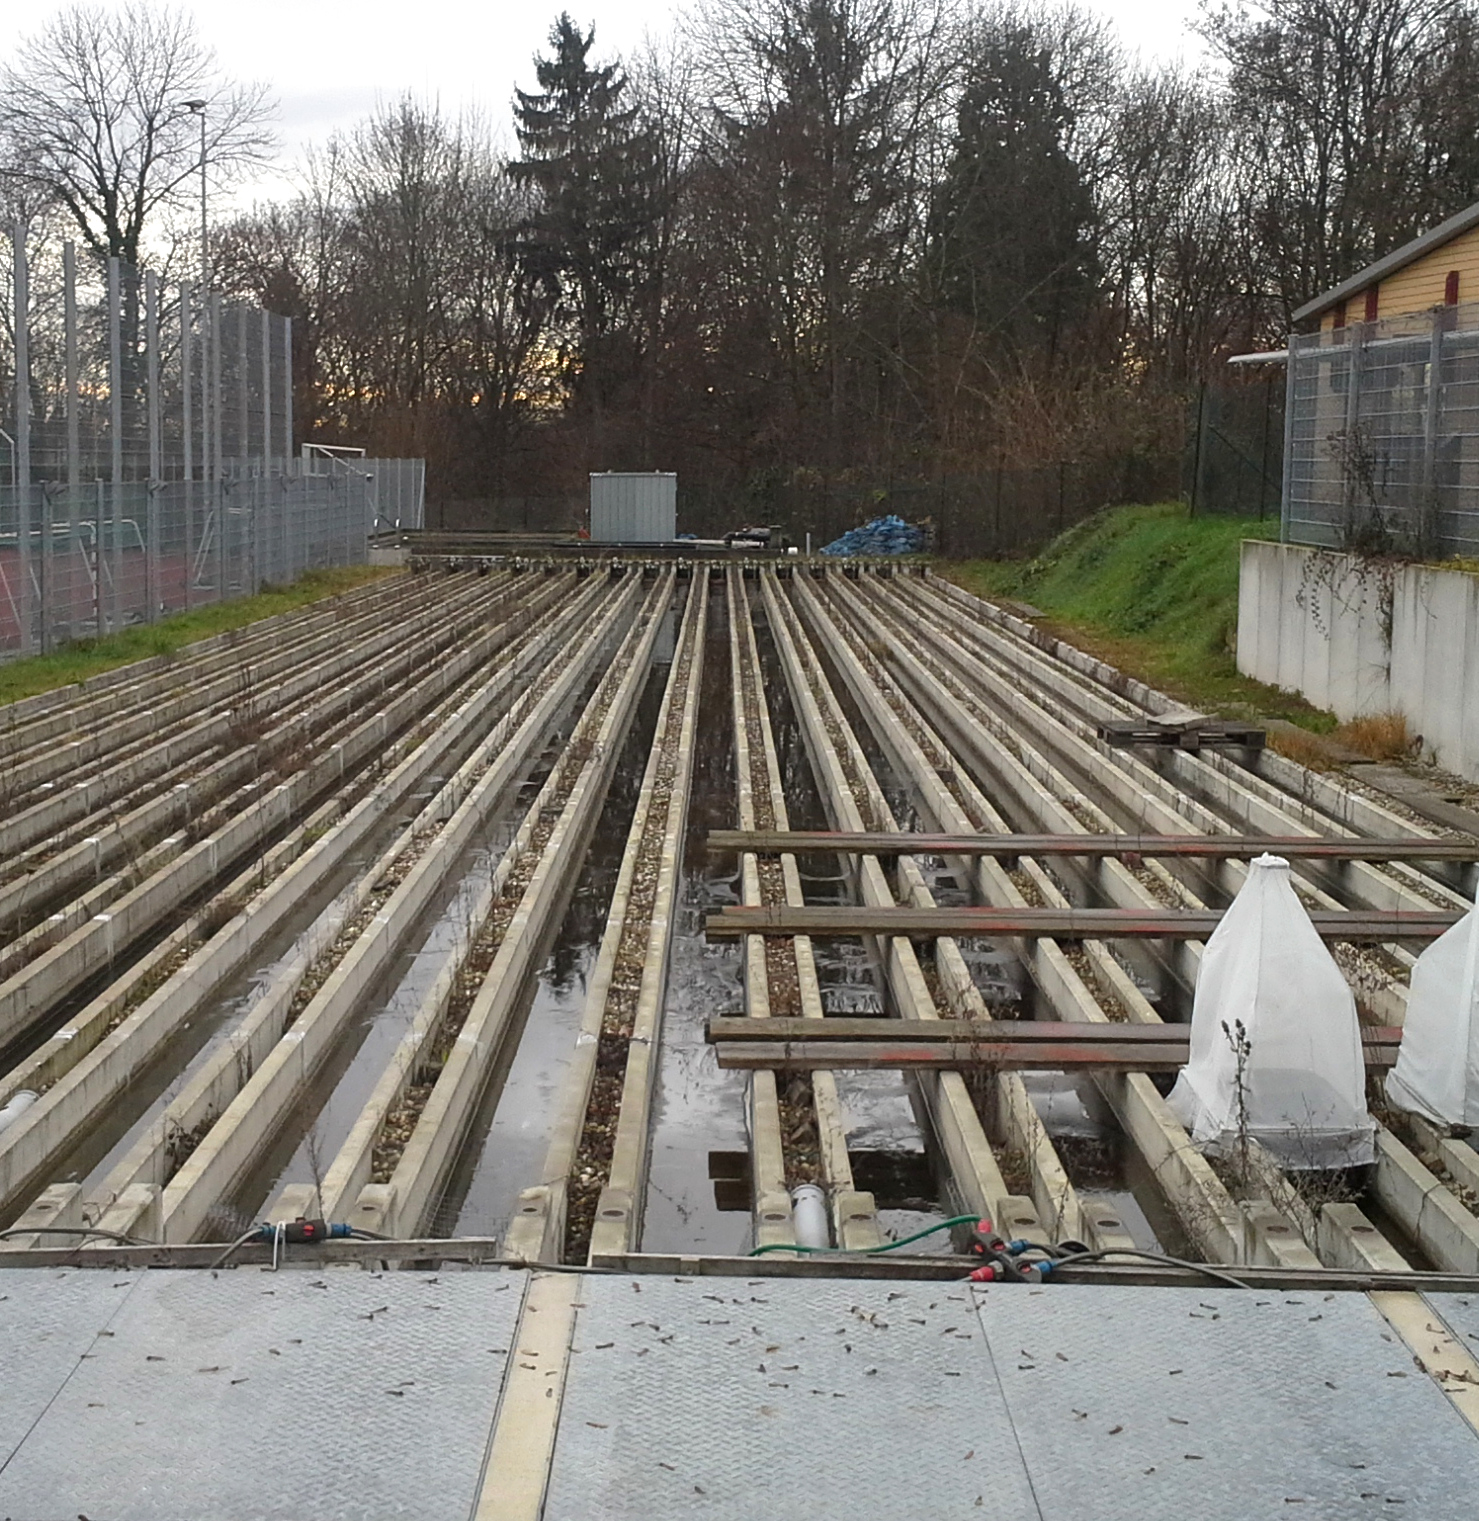
\includegraphics[width=0.9\textwidth]{figs/mesocosm_ld.jpg}
	\end{columns}

	\vfill
	\begin{columns}[T]
	\column<1->{.49\textwidth}
		\begin{itemize}
			\item Daphnia Test
			% \item Lower Tier 
			\item \emph{"x out of n survived"}
			% \item $EC_{50}$ / NOEC
		\end{itemize}

	\column<2->{.49\textwidth}
		\begin{itemize}
			\item Mesocosm
			% \item Higher Tier 
			\item \emph{"number of animals"}
			% \item NOEC
		\end{itemize}
	\end{columns}
\end{frame}
}%



\begin{frame}
\frametitle{Ecotoxicology is not normal}
\vspace*{-7mm}
	\begin{columns}[T]
	\column{.49\textwidth}
		\center
		\begin{adjustbox}{max totalsize={0.7\textwidth}{\textheight}}
					\definecolor{myblue}{rgb}{0.137, 0.251, 0.627}
\definecolor{myalert}{rgb}{0.922, 0.482, 0.078}

% overlays etc in tikz
\tikzset{
    invisible/.style={opacity=0},
    visible on/.style={alt={#1{}{invisible}}},
    alt/.code args={<#1>#2#3}{%
      \alt<#1>{\pgfkeysalso{#2}}{\pgfkeysalso{#3}} % \pgfkeysalso doesn't change the path
    },
  }

\begin{tikzpicture}[x=1pt,y=1pt]
%\definecolor{fillColor}{RGB}{255,255,255}
%\path[use as bounding box,fill=fillColor,fill opacity=0.00] (0,0) rectangle (433.62,361.35);
\begin{scope}
\path[clip] ( 18.58, 40.74) rectangle (428.12,355.85);
\path[fill=myblue] ( 37.19, 55.07) rectangle ( 59.09, 55.07);
\path[fill=myblue] ( 80.99, 55.07) rectangle (102.89, 55.14);
\path[fill=myblue] (124.79, 55.07) rectangle (146.70, 56.05);
\path[fill=myblue] (168.60, 55.07) rectangle (190.50, 62.90);
\path[fill=myblue] (212.40, 55.07) rectangle (234.30, 94.23);
\path[fill=myblue] (256.20, 55.07) rectangle (278.10,180.39);
\path[fill=myblue] (300.00, 55.07) rectangle (321.90,305.72);
\path[fill=myblue] (343.80, 55.07) rectangle (365.70,341.53);
\path[fill=myblue] (387.60, 55.07) rectangle (409.50,198.30);
\definecolor{drawColor}{RGB}{0,0,0}
\path[draw=drawColor,line width= 0.6pt,line join=round] ( 18.58, 55.07) -- (428.12, 55.07);
\end{scope}
\begin{scope}
%\path[clip] (  0.00,  0.00) rectangle (433.62,361.35);
\definecolor{drawColor}{gray}{0.30}
\node[text=drawColor,anchor=base,inner sep=0pt, outer sep=0pt, scale=  2.50] at ( 48.14, 18.58) {0};
\node[text=drawColor,anchor=base,inner sep=0pt, outer sep=0pt, scale=  2.50] at ( 91.94, 18.58) {1};
\node[text=drawColor,anchor=base,inner sep=0pt, outer sep=0pt, scale=  2.50] at (135.74, 18.58) {2};
\node[text=drawColor,anchor=base,inner sep=0pt, outer sep=0pt, scale=  2.50] at (179.55, 18.58) {3};
\node[text=drawColor,anchor=base,inner sep=0pt, outer sep=0pt, scale=  2.50] at (223.35, 18.58) {4};
\node[text=drawColor,anchor=base,inner sep=0pt, outer sep=0pt, scale=  2.50] at (267.15, 18.58) {5};
\node[text=drawColor,anchor=base,inner sep=0pt, outer sep=0pt, scale=  2.50] at (310.95, 18.58) {6};
\node[text=drawColor,anchor=base,inner sep=0pt, outer sep=0pt, scale=  2.50] at (354.75, 18.58) {7};
\node[text=drawColor,anchor=base,inner sep=0pt, outer sep=0pt, scale=  2.50] at (398.55, 18.58) {8};
 \node[text=myalert,anchor=base,inner sep=0pt, outer sep=0pt, scale=  4, font=\bf\Huge, rotate=20,
visible on=<2->] at (218, 210) {Normal?};
\end{scope}
\end{tikzpicture}

		\end{adjustbox}
		\begin{itemize}
			\item \emph{"x out of n survived"}
			% \onslide<3->{\item<ale@3-> \alert{binomial data}}
		\end{itemize}
	\column{.49\textwidth}
		\center
		\begin{adjustbox}{max totalsize={0.7\textwidth}{\textheight}}
					%\definecolor{myblue}{rgb}{0.137, 0.251, 0.627}
%\definecolor{myalert}{rgb}{0.922, 0.482, 0.078}

% overlays etc in tikz
\tikzset{
    invisible/.style={opacity=0},
    visible on/.style={alt={#1{}{invisible}}},
    alt/.code args={<#1>#2#3}{%
      \alt<#1>{\pgfkeysalso{#2}}{\pgfkeysalso{#3}} % \pgfkeysalso doesn't change the path
    },
  }


\begin{tikzpicture}[x=1pt,y=1pt]
\begin{scope}
% \path[clip] ( 18.58, 40.74) rectangle (428.12,355.85);
\path[fill=myblue] ( 37.19, 55.07) rectangle ( 71.04,198.30);
\path[fill=myblue] (104.88, 55.07) rectangle (138.73,341.53);
\path[fill=myblue] (172.58, 55.07) rectangle (206.42,341.53);
\path[fill=myblue] (240.27, 55.07) rectangle (274.12,246.04);
\path[fill=myblue] (307.96, 55.07) rectangle (341.81,150.55);
\path[fill=myblue] (375.66, 55.07) rectangle (409.50, 93.26);
\definecolor{drawColor}{RGB}{0,0,0}
\path[draw=drawColor,line width= 0.6pt,line join=round] ( 18.58, 55.07) -- (428.12, 55.07);
\end{scope}
\begin{scope}
\definecolor{drawColor}{gray}{0.30}
\node[text=drawColor,anchor=base,inner sep=0pt, outer sep=0pt, scale=  2.50] at ( 54.11, 18.58) {0};
\node[text=drawColor,anchor=base,inner sep=0pt, outer sep=0pt, scale=  2.50] at (121.81, 18.58) {1};
\node[text=drawColor,anchor=base,inner sep=0pt, outer sep=0pt, scale=  2.50] at (189.50, 18.58) {2};
\node[text=drawColor,anchor=base,inner sep=0pt, outer sep=0pt, scale=  2.50] at (257.19, 18.58) {3};
\node[text=drawColor,anchor=base,inner sep=0pt, outer sep=0pt, scale=  2.50] at (324.89, 18.58) {4};
\node[text=drawColor,anchor=base,inner sep=0pt, outer sep=0pt, scale=  2.50] at (392.58, 18.58) {5};
 \node[text=myalert,anchor=base,inner sep=0pt, outer sep=0pt, scale=  4, font=\bf\Huge, rotate=20,
visible on=<2->] at (218, 210) {Normal?};
\end{scope}
\end{tikzpicture}

		\end{adjustbox}
		\begin{itemize}
			\item \emph{"number of animals"}
			% \onslide<3->{\item<ale@3-> \alert{count data}}
		\end{itemize}
	\end{columns}

	\onslide<2->{
		\Put(90,45){\begin{adjustbox}{max totalsize={0.9\textwidth}{0.4\textheight}}
			%\definecolor{myblue}{rgb}{0.137, 0.251, 0.627}
%\definecolor{myalert}{rgb}{0.922, 0.482, 0.078}

\begin{tikzpicture}[x=1pt,y=1pt]
\definecolor{fillColor}{RGB}{255,255,255}
%\path[use as bounding box,fill=fillColor,fill opacity=0.00] (0,0) rectangle (433.62,361.35);
\begin{scope}
%\path[clip] ( 18.58, 40.74) rectangle (428.12,355.85);
\path[fill=myblue] ( 37.19, 58.25) --
	( 43.40, 59.34) --
	( 49.60, 60.75) --
	( 55.81, 62.55) --
	( 62.01, 64.82) --
	( 68.22, 67.65) --
	( 74.42, 71.15) --
	( 80.63, 75.41) --
	( 86.83, 80.54) --
	( 93.04, 86.65) --
	( 99.24, 93.84) --
	(105.45,102.18) --
	(111.65,111.76) --
	(117.86,122.60) --
	(124.06,134.71) --
	(130.27,148.07) --
	(136.48,162.58) --
	(142.68,178.12) --
	(148.89,194.50) --
	(155.09,211.50) --
	(161.30,228.81) --
	(167.50,246.13) --
	(173.71,263.08) --
	(179.91,279.28) --
	(186.12,294.34) --
	(192.32,307.87) --
	(198.53,319.50) --
	(204.73,328.92) --
	(210.94,335.85) --
	(217.14,340.10) --
	(223.35,341.53) --
	(229.55,340.10) --
	(235.76,335.85) --
	(241.96,328.92) --
	(248.17,319.50) --
	(254.37,307.87) --
	(260.58,294.34) --
	(266.78,279.28) --
	(272.99,263.08) --
	(279.19,246.13) --
	(285.40,228.81) --
	(291.61,211.50) --
	(297.81,194.50) --
	(304.02,178.12) --
	(310.22,162.58) --
	(316.43,148.07) --
	(322.63,134.71) --
	(328.84,122.60) --
	(335.04,111.76) --
	(341.25,102.18) --
	(347.45, 93.84) --
	(353.66, 86.65) --
	(359.86, 80.54) --
	(366.07, 75.41) --
	(372.27, 71.15) --
	(378.48, 67.65) --
	(384.68, 64.82) --
	(390.89, 62.55) --
	(397.09, 60.75) --
	(403.30, 59.34) --
	(409.50, 58.25) --
	(409.50, 55.07) --
	(403.30, 55.07) --
	(397.09, 55.07) --
	(390.89, 55.07) --
	(384.68, 55.07) --
	(378.48, 55.07) --
	(372.27, 55.07) --
	(366.07, 55.07) --
	(359.86, 55.07) --
	(353.66, 55.07) --
	(347.45, 55.07) --
	(341.25, 55.07) --
	(335.04, 55.07) --
	(328.84, 55.07) --
	(322.63, 55.07) --
	(316.43, 55.07) --
	(310.22, 55.07) --
	(304.02, 55.07) --
	(297.81, 55.07) --
	(291.61, 55.07) --
	(285.40, 55.07) --
	(279.19, 55.07) --
	(272.99, 55.07) --
	(266.78, 55.07) --
	(260.58, 55.07) --
	(254.37, 55.07) --
	(248.17, 55.07) --
	(241.96, 55.07) --
	(235.76, 55.07) --
	(229.55, 55.07) --
	(223.35, 55.07) --
	(217.14, 55.07) --
	(210.94, 55.07) --
	(204.73, 55.07) --
	(198.53, 55.07) --
	(192.32, 55.07) --
	(186.12, 55.07) --
	(179.91, 55.07) --
	(173.71, 55.07) --
	(167.50, 55.07) --
	(161.30, 55.07) --
	(155.09, 55.07) --
	(148.89, 55.07) --
	(142.68, 55.07) --
	(136.48, 55.07) --
	(130.27, 55.07) --
	(124.06, 55.07) --
	(117.86, 55.07) --
	(111.65, 55.07) --
	(105.45, 55.07) --
	( 99.24, 55.07) --
	( 93.04, 55.07) --
	( 86.83, 55.07) --
	( 80.63, 55.07) --
	( 74.42, 55.07) --
	( 68.22, 55.07) --
	( 62.01, 55.07) --
	( 55.81, 55.07) --
	( 49.60, 55.07) --
	( 43.40, 55.07) --
	( 37.19, 55.07) --
	cycle;
\definecolor{drawColor}{RGB}{0,0,0}

\path[draw=drawColor,line width= 0.6pt,line join=round] ( 37.19, 58.25) --
	( 43.40, 59.34) --
	( 49.60, 60.75) --
	( 55.81, 62.55) --
	( 62.01, 64.82) --
	( 68.22, 67.65) --
	( 74.42, 71.15) --
	( 80.63, 75.41) --
	( 86.83, 80.54) --
	( 93.04, 86.65) --
	( 99.24, 93.84) --
	(105.45,102.18) --
	(111.65,111.76) --
	(117.86,122.60) --
	(124.06,134.71) --
	(130.27,148.07) --
	(136.48,162.58) --
	(142.68,178.12) --
	(148.89,194.50) --
	(155.09,211.50) --
	(161.30,228.81) --
	(167.50,246.13) --
	(173.71,263.08) --
	(179.91,279.28) --
	(186.12,294.34) --
	(192.32,307.87) --
	(198.53,319.50) --
	(204.73,328.92) --
	(210.94,335.85) --
	(217.14,340.10) --
	(223.35,341.53) --
	(229.55,340.10) --
	(235.76,335.85) --
	(241.96,328.92) --
	(248.17,319.50) --
	(254.37,307.87) --
	(260.58,294.34) --
	(266.78,279.28) --
	(272.99,263.08) --
	(279.19,246.13) --
	(285.40,228.81) --
	(291.61,211.50) --
	(297.81,194.50) --
	(304.02,178.12) --
	(310.22,162.58) --
	(316.43,148.07) --
	(322.63,134.71) --
	(328.84,122.60) --
	(335.04,111.76) --
	(341.25,102.18) --
	(347.45, 93.84) --
	(353.66, 86.65) --
	(359.86, 80.54) --
	(366.07, 75.41) --
	(372.27, 71.15) --
	(378.48, 67.65) --
	(384.68, 64.82) --
	(390.89, 62.55) --
	(397.09, 60.75) --
	(403.30, 59.34) --
	(409.50, 58.25);

\path[draw=drawColor,line width= 0.6pt,line join=round] ( 18.58, 55.07) -- (428.12, 55.07);
\end{scope}
\begin{scope}
%\path[clip] (  0.00,  0.00) rectangle (433.62,361.35);
\definecolor{drawColor}{gray}{0.30}
\node[text=drawColor,anchor=base,inner sep=0pt, outer sep=0pt, scale=  2.50] at ( 37.19, 18.58) {-1};
\node[text=drawColor,anchor=base,inner sep=0pt, outer sep=0pt, scale=  2.50] at ( 99.24, 18.58) {0};
\node[text=drawColor,anchor=base,inner sep=0pt, outer sep=0pt, scale=  2.50] at (161.30, 18.58) {1};
\node[text=drawColor,anchor=base,inner sep=0pt, outer sep=0pt, scale=  2.50] at (223.35, 18.58) {2};
\node[text=drawColor,anchor=base,inner sep=0pt, outer sep=0pt, scale=  2.50] at (285.40, 18.58) {3};
\node[text=drawColor,anchor=base,inner sep=0pt, outer sep=0pt, scale=  2.50] at (347.45, 18.58) {4};
\node[text=drawColor,anchor=base,inner sep=0pt, outer sep=0pt, scale=  2.50] at (409.50, 18.58) {5};

% \node[text=myalert,anchor=base,inner sep=0pt, outer sep=0pt, scale=  5, font=\bf\Huge, rotate=20] at (218, 300) {Normal?};
\end{scope}
\end{tikzpicture}

		\end{adjustbox}
		}
	}
	\vspace*{0.5cm}
	\begin{itemize}
		\item<3-> ignore?
		\item<4-> transform?
		\item<5-> non-parametric?
		\only<6>{\item Generalised Linear Model (GLM)?}
		\onslide<7->{\item<ale@2-> \alert{Generalised Linear Model (GLM)?}}
	\end{itemize}

\end{frame}



% \begin{frame}
% \frametitle{A recent history (uncomprehensive) of GLM in ecology}
% 	% -*- root: ../../talk.tex -*-

%%% GLM History Timeline
% see als http://stackoverflow.com/questions/217834/how-to-create-a-timeline-with-latex


% http://tex.stackexchange.com/questions/55806/mindmap-tikzpicture-in-beamer-reveal-step-by-step/55849#55849
% overlays etc in tikz
\tikzset{
    invisible/.style={opacity=0},
    visible on/.style={alt={#1{}{invisible}}},
    alt/.code args={<#1>#2#3}{%
      \alt<#1>{\pgfkeysalso{#2}}{\pgfkeysalso{#3}} % \pgfkeysalso doesn't change the path
    },
  }


\begin{tikzpicture}[scale=0.57] % timeline 1990-2010->
    % define coordinates (begin, used, end, arrow)
    \foreach \x in {2010,2011,2016, 2017}{
        \pgfmathsetlength\yearposx{(\x-1990)*1cm};
        \coordinate (y\x)   at (\yearposx,0);
        \coordinate (y\x t) at (\yearposx,+3pt);
        \coordinate (y\x b) at (\yearposx,-3pt);
    }
    % draw horizontal line with arrow
    \draw [->] (y2010) -- (y2017);
     \draw[snake] (\yearposx{(2005-1990)*1cm},0) -- (\yearposx{(2010-1990)*1cm},0);


	% Nelder
    \node [ text = myalert,
 visible on=<1>
] at (\yearposx{(2006-1990)*1cm}, 0) [rotate=90,anchor=east] {1972};
    \node [
 visible on=<2->
] at (\yearposx{(2006-1990)*1cm}, 0) [rotate=90,anchor=east] {1972};
    \node [ 
 visible on=<1>
] (nelder) at (\yearposx{(2010-1990)*1cm}, 5)  {
\includegraphics[width=10cm]{/home/edisz/Documents/work/research/projects/2016/1PHD/phd_defense/figs/tikz/glm_hist/nelder.png}};

	% oHara
    \node [ text = myalert,
 visible on=<2>
] at (\yearposx{(2010-1990)*1cm}, 0) [rotate=90,anchor=east] {2010};
    \node [ 
 visible on=<3->
] at (\yearposx{(2010-1990)*1cm}, 0) [rotate=90,anchor=east] {2010};
	\draw  [ 
 visible on=<2->
] (\yearposx{(2010-1990)*1cm}, 3pt) --  (\yearposx{(2010-1990)*1cm}, -3pt);
    \node [ 
 visible on=<2>
] (ohara) at (\yearposx{(2010-1990)*1cm}, 5)  {
\includegraphics[width=10cm]{/home/edisz/Documents/work/research/projects/2016/1PHD/phd_defense/figs/tikz/glm_hist/ohara_2010.png}};

	% warton & Hui
    \node [ text=myalert,
 visible on=<3>
] at (\yearposx{(2011-1990)*1cm}, 0) [rotate=90,anchor=east] {2011};
    \node [ 
 visible on=<4->
] at (\yearposx{(2011-1990)*1cm}, 0) [rotate=90,anchor=east] {2011};
	\draw  [ 
 visible on=<3->
] (\yearposx{(2011-1990)*1cm}, 3pt) --  (\yearposx{(2011-1990)*1cm}, -3pt);
    \node [ 
 visible on=<3>
] (ohara) at (\yearposx{(2010-1990)*1cm}, 5)  {
\includegraphics[width=10cm]{/home/edisz/Documents/work/research/projects/2016/1PHD/phd_defense/figs/tikz/glm_hist/warton_2011.png}};

	% warton mvglm
    \node [ text=myalert,
 visible on=<4>
] at (\yearposx{(2012-1990)*1cm}, 0) [rotate=90,anchor=east] {2012};
    \node [ 
 visible on=<5->
] at (\yearposx{(2012-1990)*1cm}, 0) [rotate=90,anchor=east] {2012};
	\draw  [ 
 visible on=<4->
] (\yearposx{(2012-1990)*1cm}, 3pt) --  (\yearposx{(2012-1990)*1cm}, -3pt);
    \node [ 
 visible on=<4>
] (ohara) at (\yearposx{(2010-1990)*1cm}, 5)  {
\includegraphics[width=10cm]{/home/edisz/Documents/work/research/projects/2016/1PHD/phd_defense/figs/tikz/glm_hist/warton_2012.png}};

	% Szoecs, mesocosm
    \node [ text=myalert,
 visible on=<5->
] at (\yearposx{(2015-1990)*1cm}, 0) [rotate=90,anchor=east] {2015};
	\draw  [ 
 visible on=<5->
] (\yearposx{(2015-1990)*1cm}, 3pt) --  (\yearposx{(2015-1990)*1cm}, -3pt);
    \node [ 
 visible on=<5>
] (ohara) at (\yearposx{(2010-1990)*1cm}, 5)  {
\includegraphics[width=10cm]{/home/edisz/Documents/work/research/projects/2016/1PHD/phd_defense/figs/tikz/glm_hist/Szoecs_2015.png}};

	% Szoecs, normal
    \node [ 
 visible on=<6>
] (ohara) at (\yearposx{(2010-1990)*1cm}, 5)  {
\includegraphics[width=10cm]{/home/edisz/Documents/work/research/projects/2016/1PHD/phd_defense/figs/tikz/glm_hist/Szoecs_2015_notnormal.png}};


\end{tikzpicture}

% \end{frame}


\begin{frame}[t]
\frametitle{GLMs may have better properties}
\begin{tabular}{llll}
\textbf{Model} & \textbf{Observations} & \textbf{Predictors} & \textbf{Link} \\ \hline
LM & Y \textasciitilde~N(μ, R) & η =Xβ & η = μ \\ \pause
\alert{GLM} & Y \textasciitilde~\alert{G}(μ, R) & η =Xβ & η = \alert{g(}μ\alert{)} \\ 
% LMM & Y|b \textasciitilde~N(μ, R) & η =Xβ + Zb , b \textasciitilde~N(0, G) & η = μ \\ 
% GLMM & Y|b \textasciitilde~G(μ, R) & η =Xβ + Zb , b \textasciitilde~N(0, G) & η = g(μ) \\ 
\end{tabular}
\vspace*{0.5em}
\pause
\setlength{\fboxsep}{1pt}
\fcolorbox{myalert}{myalert}{
\includegraphics[width=\textwidth]{figs/tikz/glm_hist/ohara_2010.png}} \\[0.5em]
\fcolorbox{myalert}{myalert}{
\includegraphics[width=\textwidth]{figs/tikz/glm_hist/warton_2011.png}}
\end{frame}


\begin{frame}
\frametitle{GLMs in Ecotoxicology?}
	\setlength{\fboxsep}{1pt}
	\only<1-2>{
		\fcolorbox{gray}{gray}{
\includegraphics[width=\textwidth]{figs/oecd_2006.png}}\\
	}
	\only<2>{
		\Put(25, 290){\alert{\Huge\textbf{"GLMs are not discussed}}}
		}
	\only<2>{
		\Put(30, 240){\alert{\Huge\textbf{in this document."}}}
		}
	\onslide<4>{
		\alert{\Huge\textbf{No reference to GLM.}}
		}
	\onslide<3-4>{
		
\includegraphics[width=0.8\textwidth]{figs/quant_ecotox.jpg}\\
	}
\end{frame}


\begin{frame}[t]
\frametitle{Method: Simulations}

	\only<1>{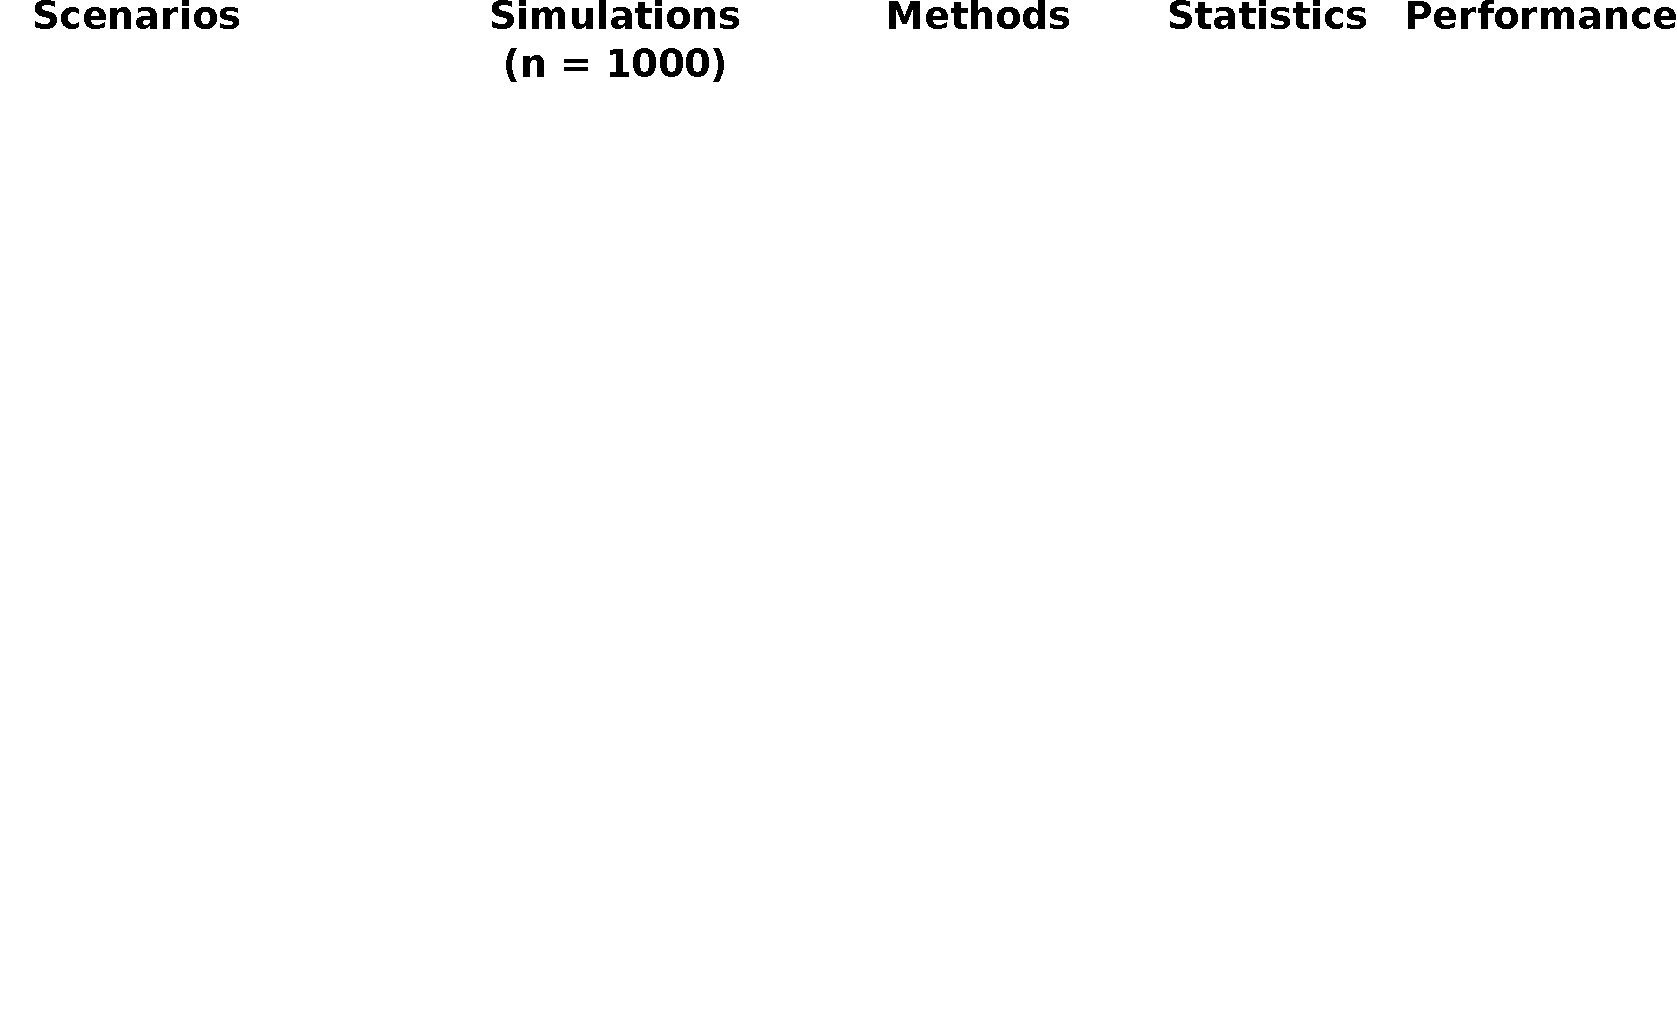
\includegraphics[width=\textwidth]{figs/power/power_methods_1.pdf}}
	\only<2>{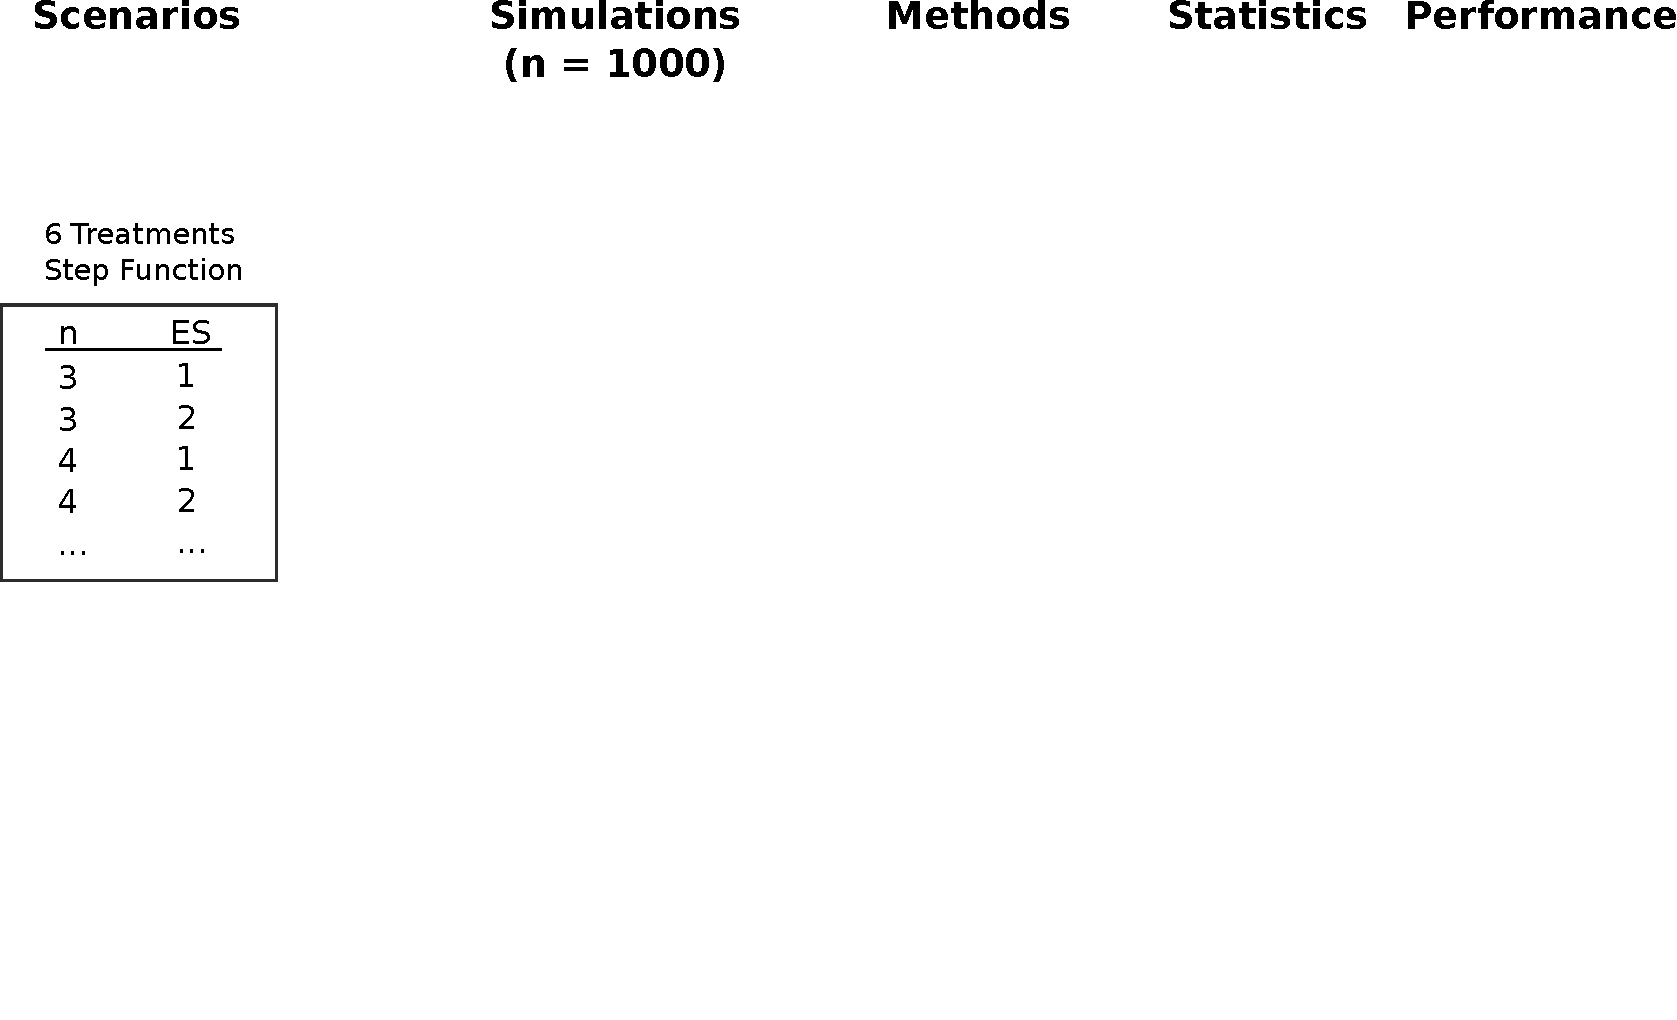
\includegraphics[width=\textwidth]{figs/power/power_methods_2.pdf}}
	\only<3-4>{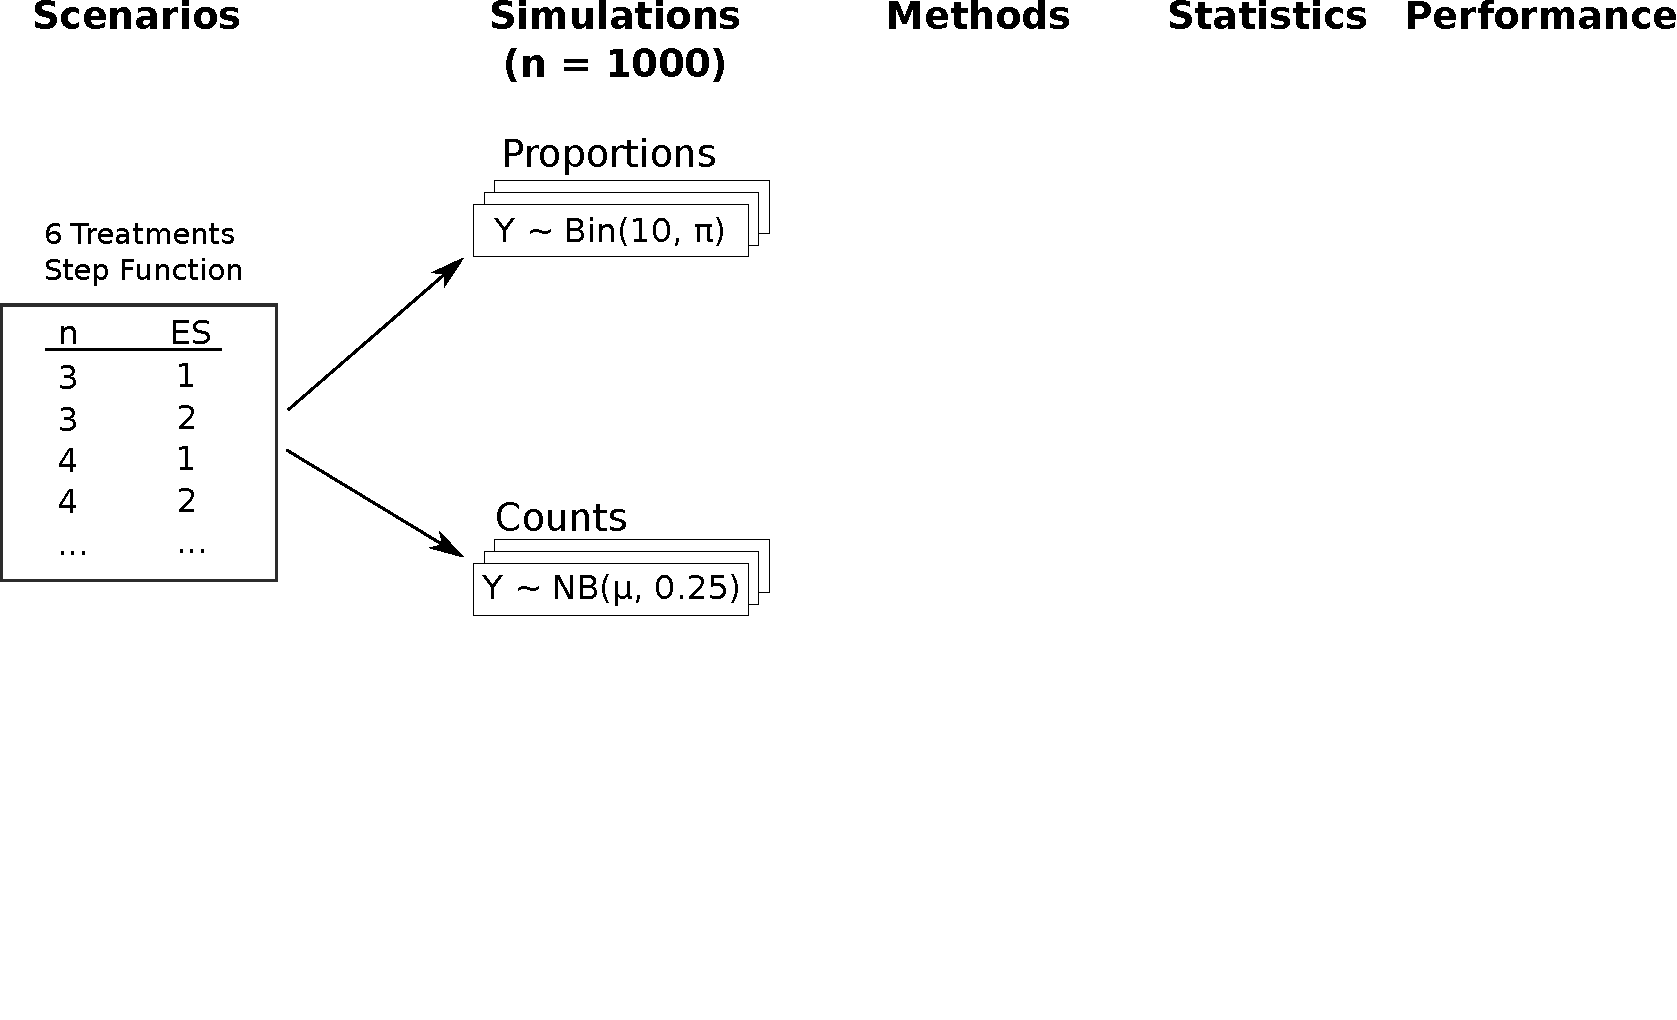
\includegraphics[width=\textwidth]{figs/power/power_methods_3.pdf}}
	\only<5>{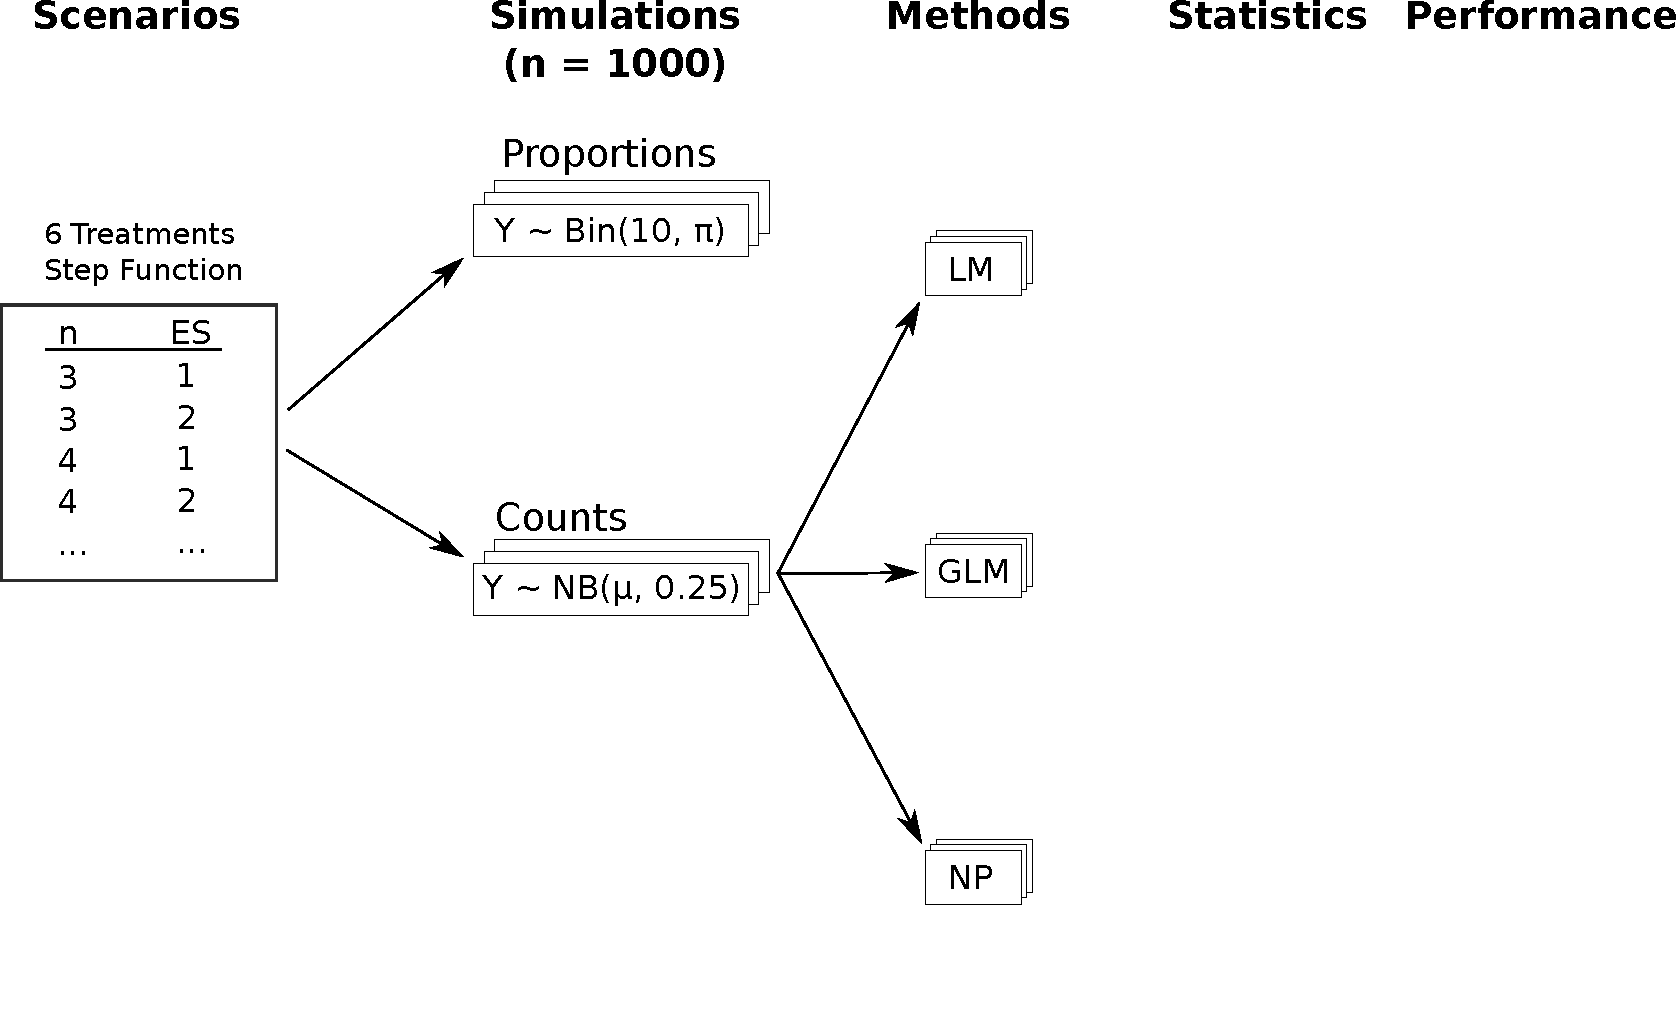
\includegraphics[width=\textwidth]{figs/power/power_methods_4.pdf}}
	\only<6>{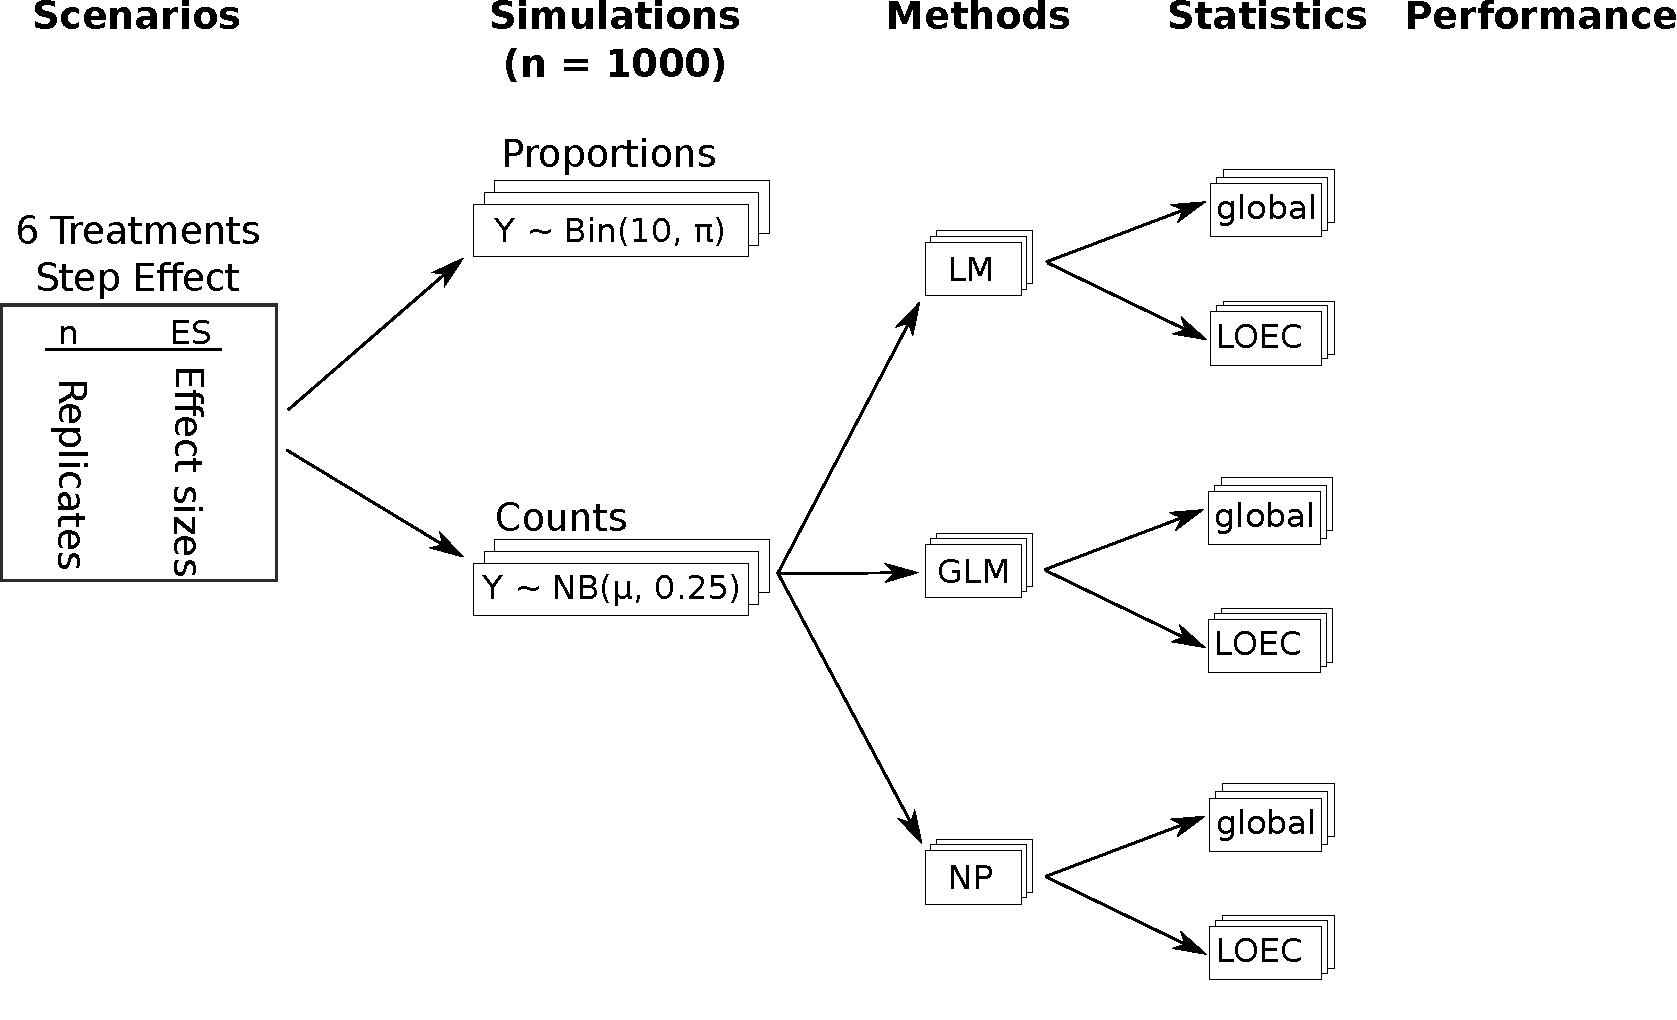
\includegraphics[width=\textwidth]{figs/power/power_methods_5.pdf}}
	\only<7>{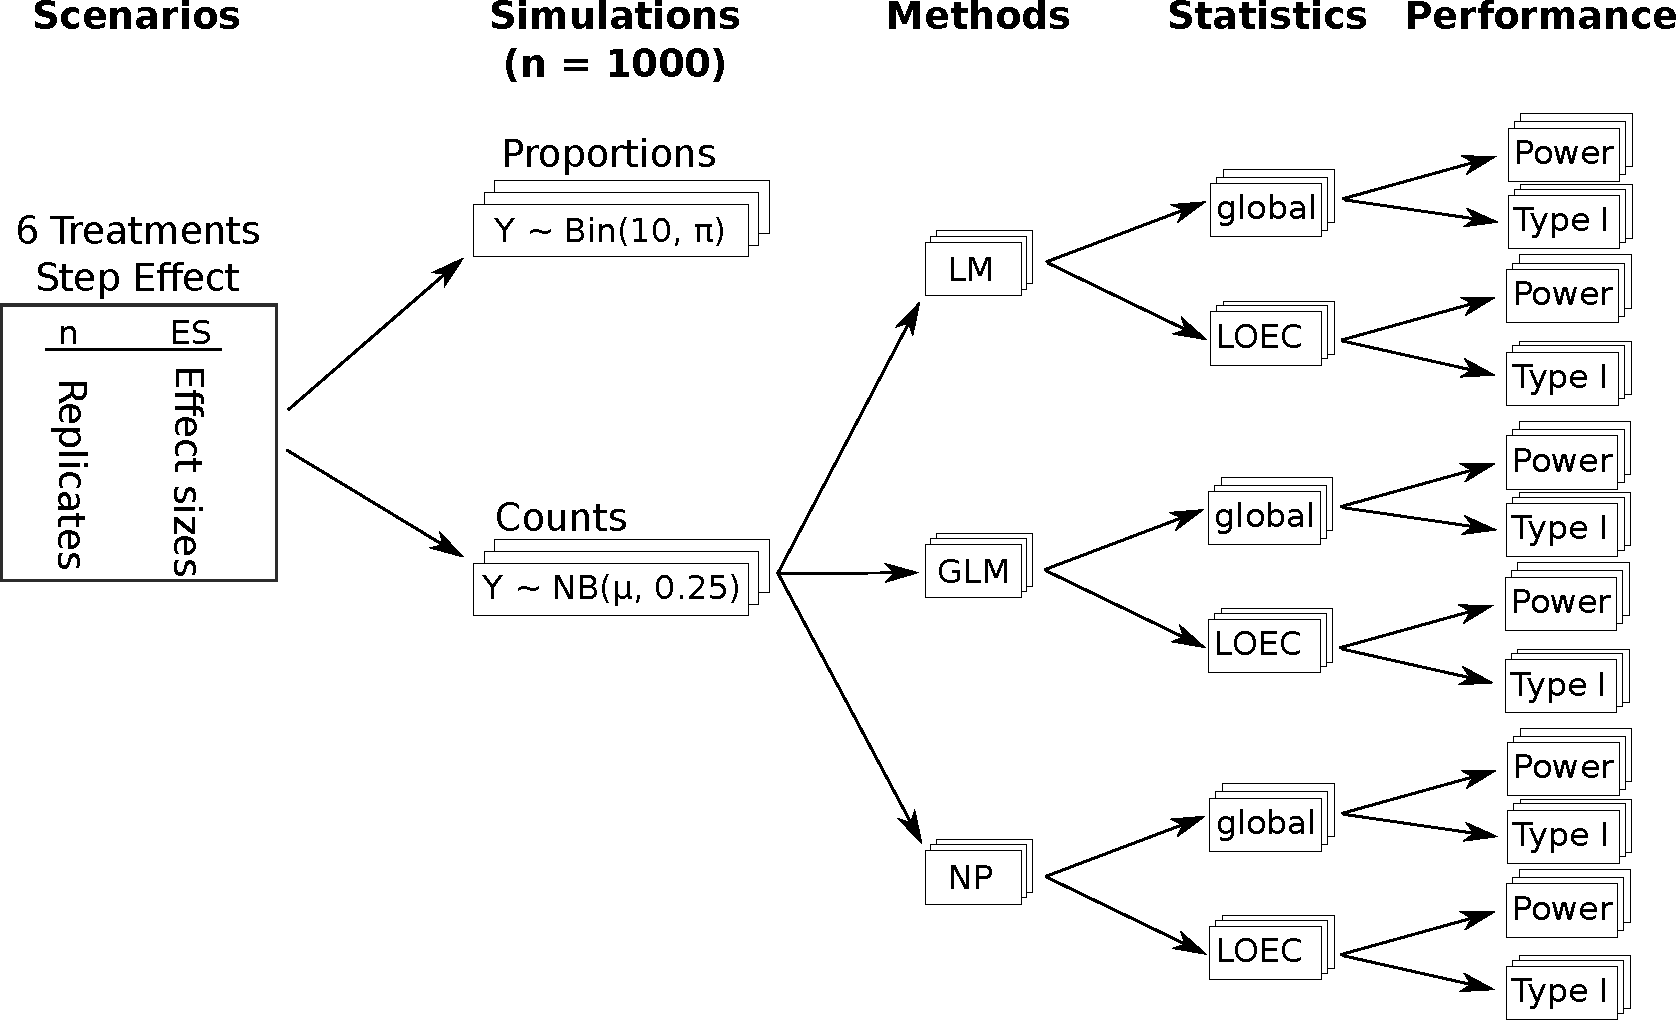
\includegraphics[width=\textwidth]{figs/power/power_methods_all.pdf}}

	\setlength{\fboxsep}{1pt}
	\only<4-5>{\Put(-30, 200){
		\fcolorbox{myalert}{myalert}{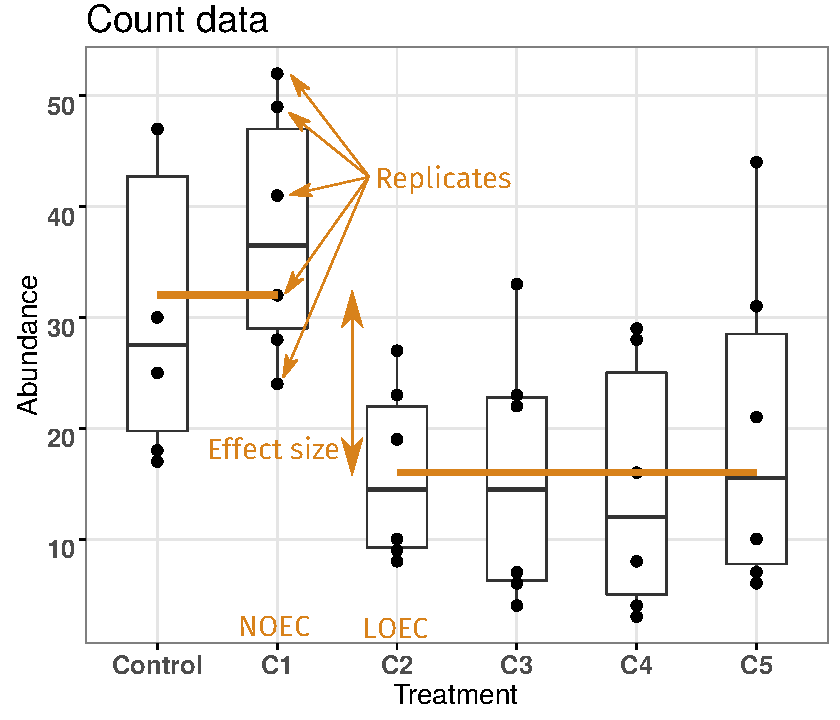
\includegraphics[width=0.55\textwidth]{figs/p_sim_fin.pdf}}
	}}
	\only<6->{\Put(-30, 166.5){
		\fcolorbox{myalert}{myalert}{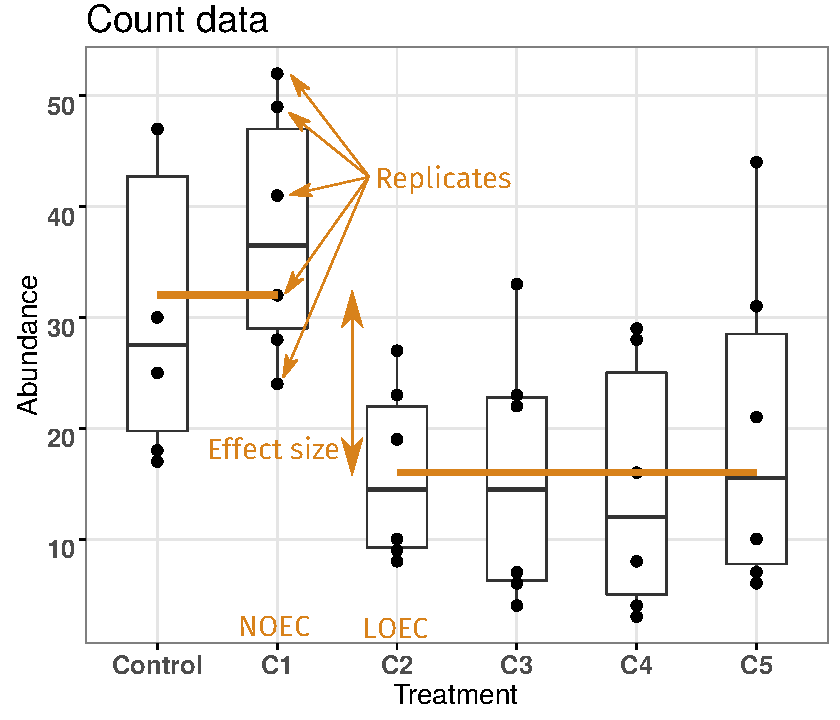
\includegraphics[width=0.55\textwidth]{figs/p_sim_fin.pdf}}
	}}
\end{frame}




\begin{frame}
\frametitle{Type I Errors: GLMs can fail}
	\begin{center}
		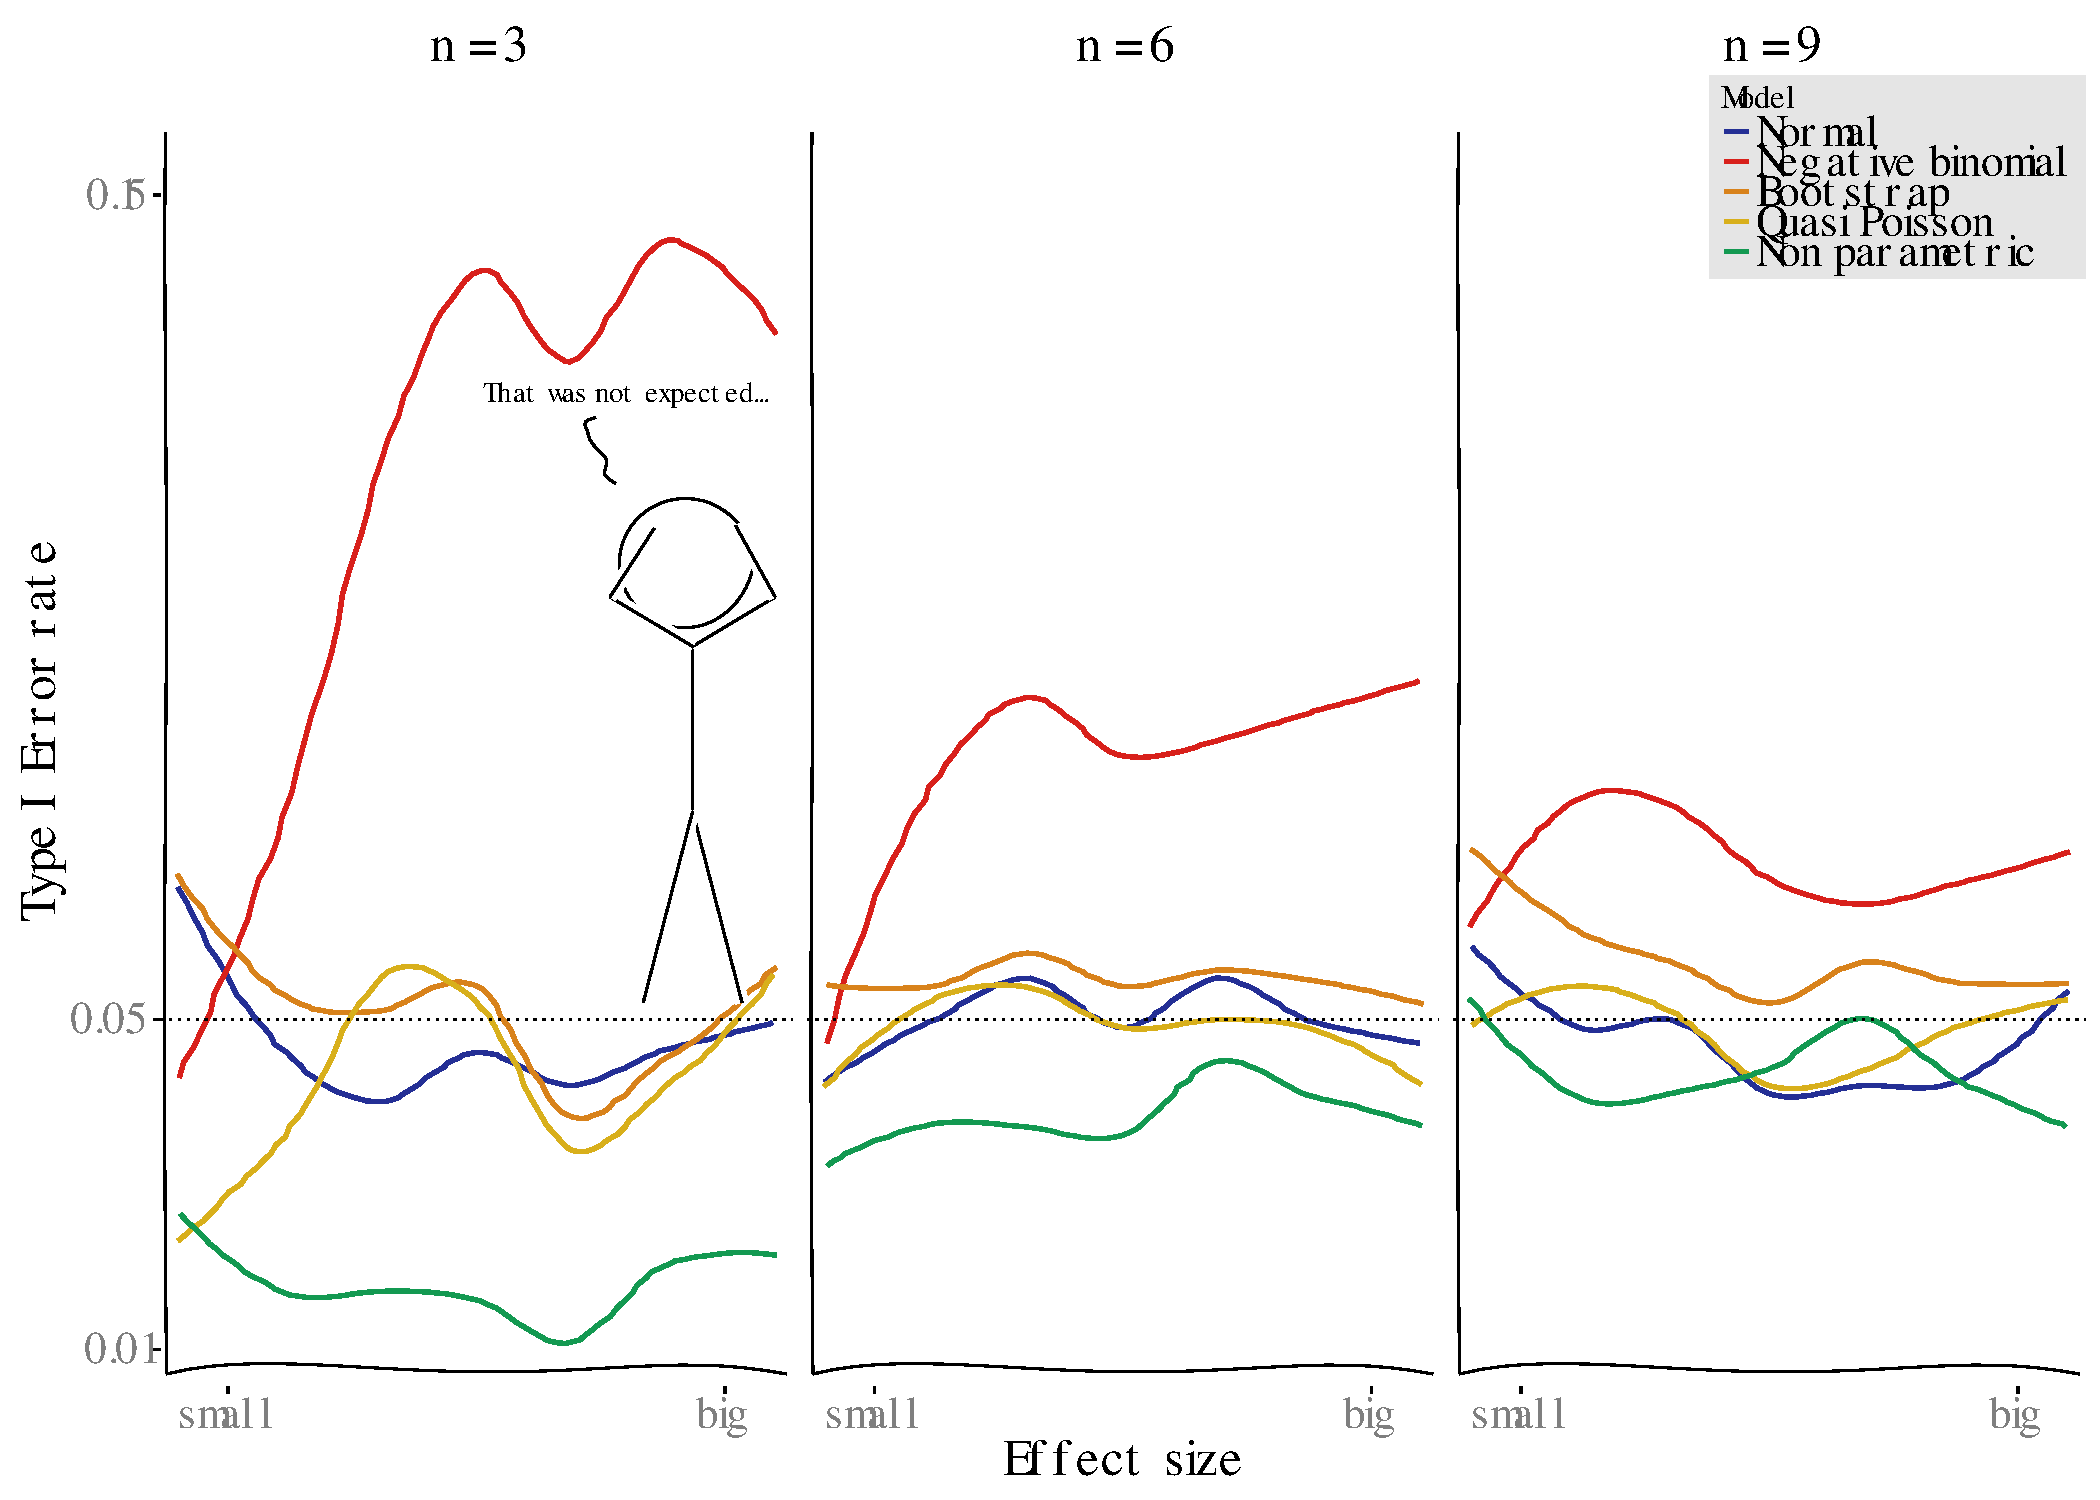
\includegraphics[width=\textwidth]{figs/p_t1_xkcd.pdf}
	\end{center}
\end{frame}


\begin{frame}
\frametitle{Power: But GLMs can do also better}
	\begin{center}
		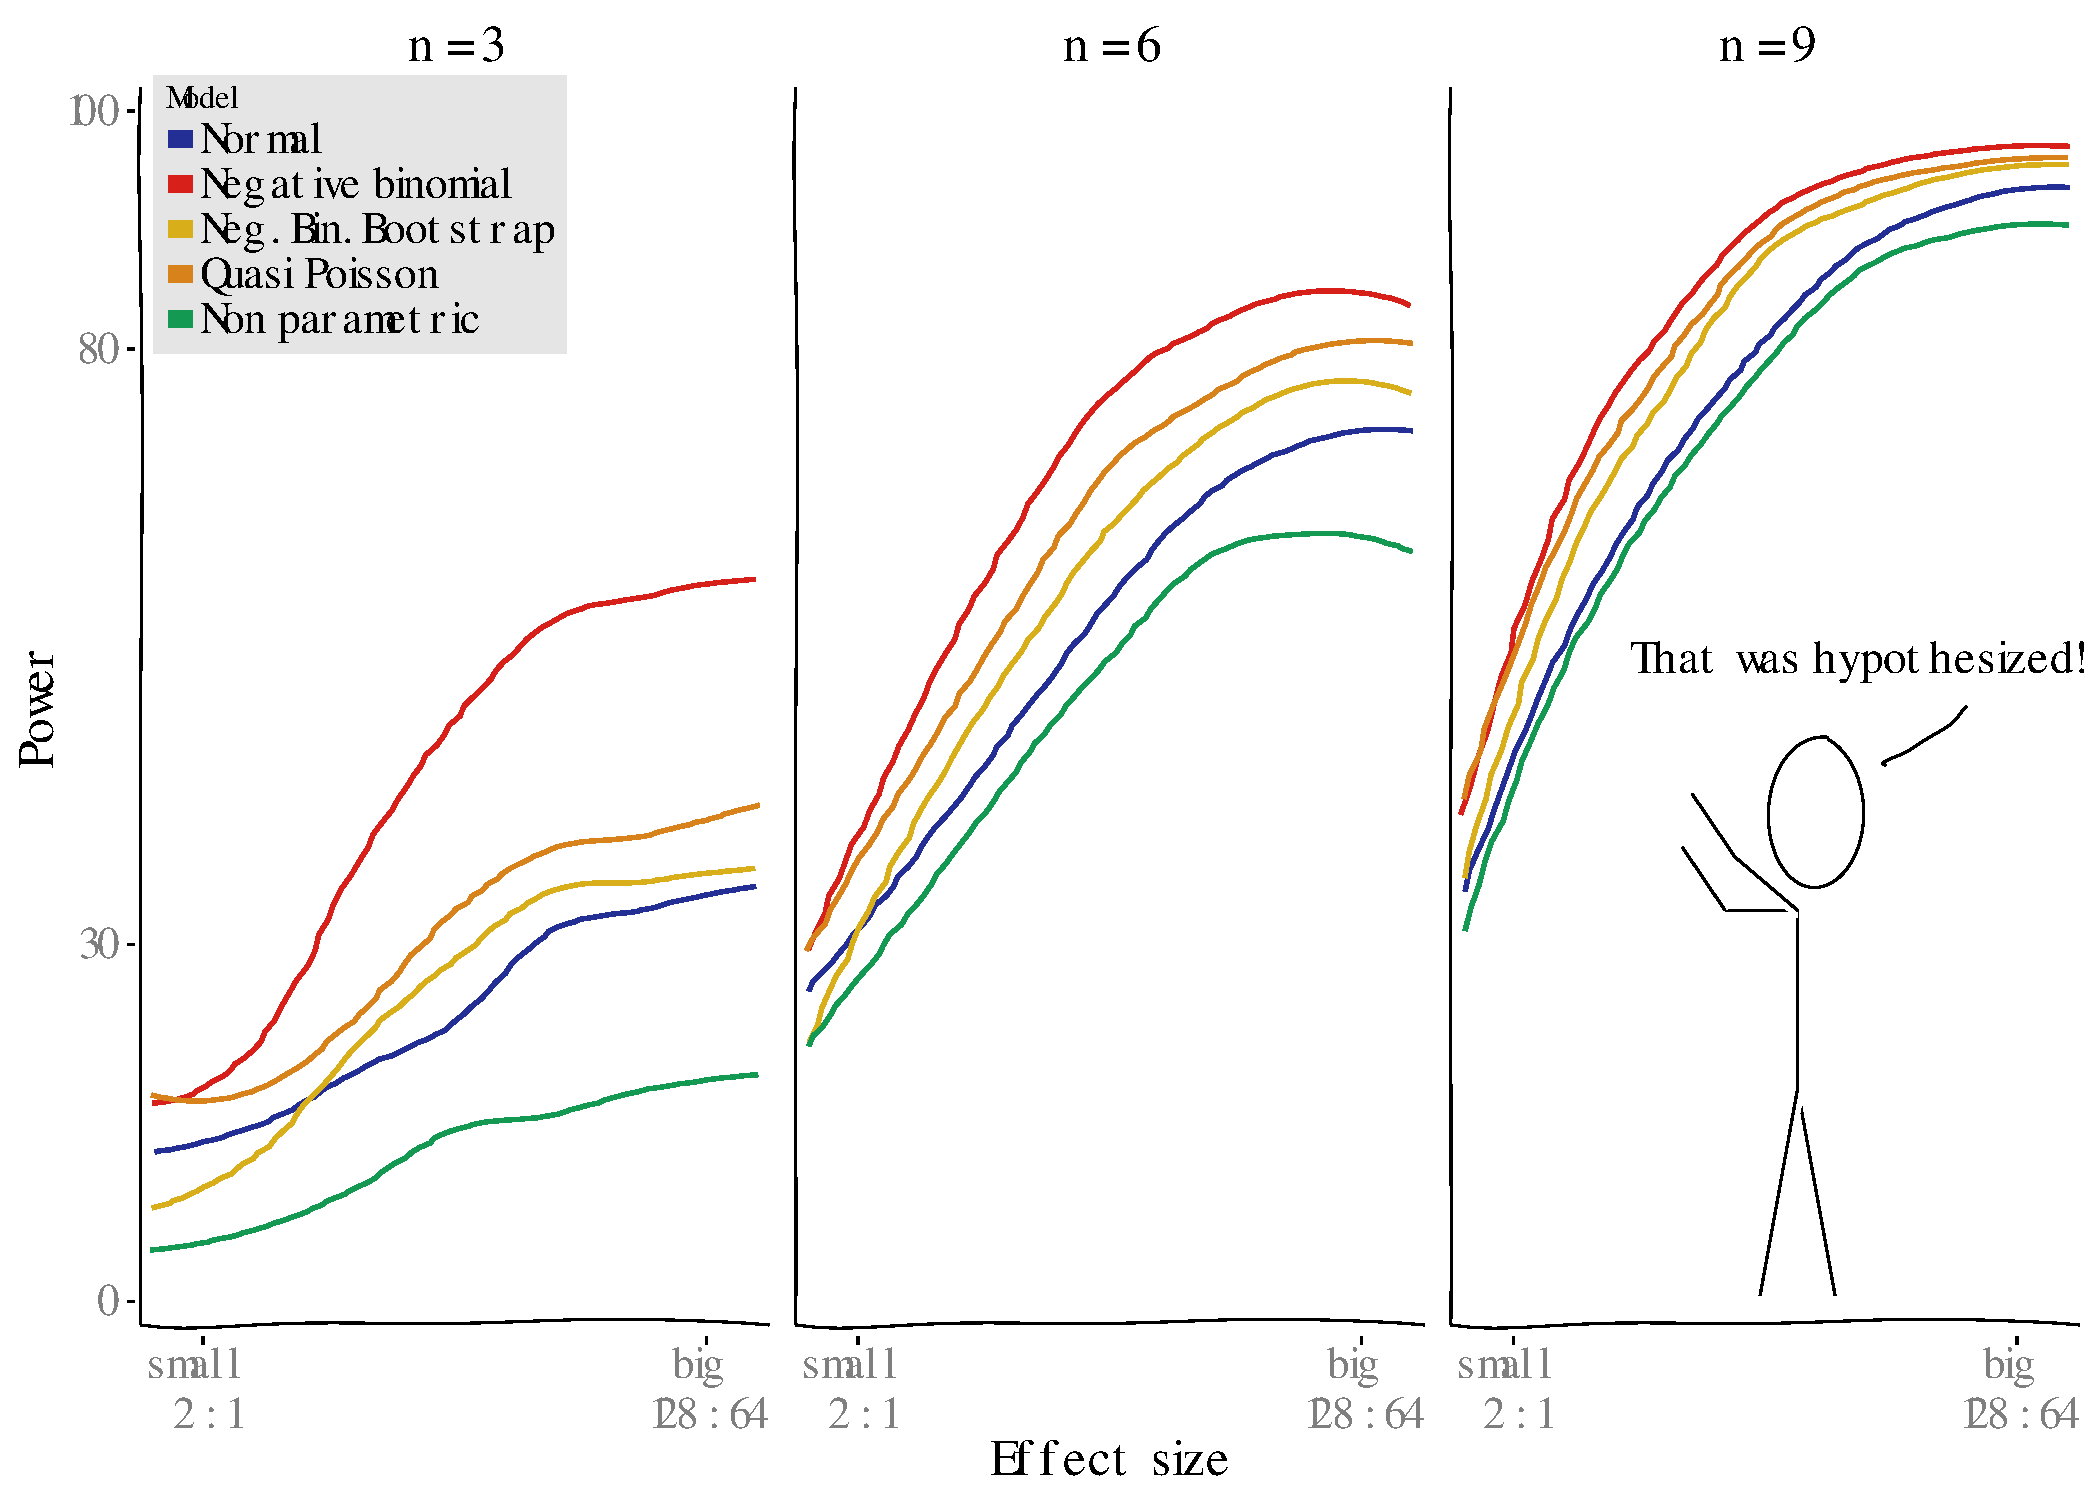
\includegraphics[width = \textwidth]{figs/p_pow_xkcd.pdf}
	\end{center}
\end{frame}



\begin{frame}
\frametitle{What we learned from this study}
	\metroset{block=fill}
		\begin{enumerate}
			\item Negative-binomial GLM show increased \alert{Type I errors}
			\item Can be fixed via \alert{bootstrap}
			\item Ecotoxicological experiments commonly \alert{low power} 
			\item \alert{GLMs} can increase this  power
		\end{enumerate}
\end{frame}



\begin{frame}
\frametitle{Where are we today?}
	
\includegraphics[width=\textwidth]{figs/tikz/glm_hist/warton_2016.png}
	\pause
	\vspace*{-5mm}
	\metroset{block=fill}
	\begin{exampleblock}{State of the art}
		\begin{enumerate}
			\item Choose your model based on data properties
			\item Fix Type I errors by resampling
			\item GLMs have greater power 
		\end{enumerate}
	\end{exampleblock}
\end{frame}




\begingroup
\footnotesize % = 10pt in 12pt default
\begin{frame}
\frametitle{Identifying Risks using Monitoring Data}
    \vspace*{5mm}
	\resizebox{1.1\textwidth}{!}{
		\hspace*{-20mm}% -*- root: ../../talk.tex -*-

% Define elements
% arrows, see also http://tex.stackexchange.com/questions/5461/is-it-possible-to-change-the-size-of-an-arrowhead-in-tikz-pgf/161238#161238
\tikzstyle{line} = [draw, -{Latex[length=4mm,width=3mm]}, ultra thick]
% rectangles
\tikzstyle{block} = [rectangle, draw, 
    text width=5em, text centered, rounded corners, minimum height=4em]
% papers
\tikzstyle{paper} = [circle, draw, fill=myalert,  font = \bf\LARGE, minimum width=1.5cm]
\tikzstyle{textbf} = [text centered, font = \bf\large]

% http://tex.stackexchange.com/questions/55806/mindmap-tikzpicture-in-beamer-reveal-step-by-step/55849#55849
% overlays etc in tikz
\tikzset{
    invisible/.style={opacity=0},
    visible on/.style={alt={#1{}{invisible}}},
    alt/.code args={<#1>#2#3}{%
      \alt<#1>{\pgfkeysalso{#2}}{\pgfkeysalso{#3}} % \pgfkeysalso doesn't change the path
    },
  }

 \definecolor{ao}{rgb}{0.00, 0.40, 0.60}
% \usetikzlibrary{shapes, arrows, positioning, calc, arrows.meta, snakes}
% \definecolor{myalert}{rgb}{0.922, 0.482, 0.078}


\begin{tikzpicture}[node distance = 2cm, auto]
	
% clip figure
\clip(-1.5, -10.5) rectangle (21.0, 3.5);

% % % % % grid for coordinates for clip
\draw[help lines,xstep=1,ystep=1] (-2,-13) grid (30,6.5);
\foreach \x in {-2,-1,...,30} { \node [anchor=north] at (\x,0) {\x}; }
\foreach \y in {-13,-12,...,6} { \node [anchor=east] at (0,\y) {\y}; }


% Nodes
	%% Effects
	\node [name = exp, block, minimum width=2cm] {Experiment} ;
	\node [name = stat, block, minimum width=2cm, right=1cm of exp] {Data / Statistics} ;
    \node [name = eff, block, 
		minimum width=57mm, 
		minimum height=25mm, 
		below left=5mm of exp.west, anchor = west] {} ;
	\node[textbf, below right=8mm and 5mm of exp, anchor = south]{Effects};

	%% Exposure
  	\node [name = prop, block, minimum width=2cm, below=38mm of exp] {Data / Properties} ;
	\node [name = model, block, minimum width=2cm, right=1cm of prop] {Models} ;
	\node [name = expo, block, 
		minimum width=57mm, 
		minimum height=25mm, 
		below = 20mm of eff] {} ;
	\node[textbf, above=-2mm of expo, anchor = north]{Exposure};

	%% Risk Assessment
	\node [name = risk, block, below right=0.6cm and 1cm of stat,
       minimum width=45mm, 
		minimum height=2.5cm, 
		font = \bf\large,
		align = center,
       text width = 3cm,
       color=myalert,
       visible on=<1->] {Environmental Risk\\  Assessment};

	%% Monitoring data
	\node [name = monit, block, 
		right = 7.5cm of risk,
        minimum width=35mm, 
		minimum height=20mm, 
		font = \bf\large,
		align = center,
        text width = 3.5cm,
        visible on=<1->] {Environmental\\ Monitoring};

	%% biological data
	\node [name = bio, block, 
		above left = 2cm and 2cm of monit, anchor = north,
		minimum width=30mm, align = center, text width = 30mm, font=\large] {Biology   };
	%% chemical data
	\node [name = chem, block, 
		below left = 2cm and 2cm of monit, anchor = south,
		minimum width=3cm, font=\large,text width = 30mm,
		color=myalert] { Chemistry};

	%% Legislation
   \node[name=dir, above= 10mm of eff, font=\large, text width = 60mm, fill = ao, text=white, xshift=10mm,
   visible on=<1->]{\textbf{Plant Protection Products Regulation 1107/2009}};
   \node[name=wfd, right= 80mm of dir, font=\large, text width = 65mm, 
   fill = ao, text=white,
   visible on=<1->]{\textbf{Water Framework Directive 2000/60/EC}};


  %% Papers
  	\node[name = chap2, paper, 
		above left = 5mm and -15mm of stat, 
		anchor = east, fill=lightgray]{1};	
    \node[name = chap3, paper, 
		below left = -22mm and 0mm of chem, anchor = north
		]{2};
	\node[name = chap3a, paper, 
		below = 15mm of expo, 
		anchor = east]{2};	
	\node[name = chap3t, right = 5mm of chap3a, font = \bf\large, color = myalert, text width = 180mm]{Szöcs, Brinke, Karaoglan \& Schäfer (in revision). “Large scale risks from pesticides in small streams”. Environmental Science \& Technology.};

% arrows
	\path [line] (prop) -- (model);
		\path [line] (expo) -| node[pos = 0.4, font = \large,  below]{PEC} (risk);
		\path [line] (exp) -- (stat);
	\path [line] (eff) -| node[pos = 0.4, font = \large]{RAC} (risk);
	\path [line] (monit) |- (bio);
	\path [line] (monit) |- (chem);
	\path [dashed,
	visible on=<1->] (risk.south east) edge [line ,bend right = 40, color=myalert]  node [xshift = -4mm, yshift = -7mm, pos =0.1, below, font = \large, align = center, color = black] {Approves \\ Substance} (chem);
	\path [dashed] ([yshift=5mm]bio.south west) edge[line, bend left = -10]   ([yshift=0mm]risk.north east);
    \path [dashed] (chap3.north west) edge [line, bend right = 30, color = myalert] node[xshift = 20mm, yshift =11mm, font = \large, align = center, color = black] {Retrospection}  (risk);

    \node[name = PECabbrv, 
		below left = 30mm and -2mm of expo, 
		font=\normalsize, 
		anchor = west]{\textbf{RAC:}~~Regulatory Acceptable Concentration};	
	\node[name = RACabbrv, 
		below = 0mm of PECabbrv, xshift = 2mm, 
		font=\normalsize, 
		anchor = north]{\textbf{PEC:}~~Predicted Environmental Concentration};

\end{tikzpicture}

	}
\end{frame}
\endgroup



%%% ---------------------------------------------------------------------------
\section{Identifying Risks using Monitoring Data}


\begin{frame}
\frametitle{Goals \& Hypotheses}
	\metroset{block=fill}
	\begin{exampleblock}{Goal: Combine monitoring and ERA}
		\begin{itemize}
			\item Compile nation-wide monitoring data % (federalism)
			\item Focus on pesticides
			\item Focus on small streams
			\item Identify risks \& influencing factors
		\end{itemize}
	\end{exampleblock}
	\pause
	\begin{exampleblock}{Hypotheses}
		\begin{enumerate}
			% \item Agricultural streams show highest concentrations
			% \item Small streams with highest concentrations
			% \item Precipitation increases concentrations
			% \item Highest concentrations in summer
			% % \item Mainly insecticides responsible for risks
			\item Agriculture:~~~~~\textbf{\Large\textuparrow}~~~~~Concentration: \textbf{\Large\textuparrow}
			\pause
			\item Stream size:~~~~\textbf{\Large\textdownarrow}~~~~~Concentration: \textbf{\Large\textuparrow}
			\pause
			\item Precipitation:~~\textbf{\Large\textuparrow}~~~~~Concentration: \textbf{\Large\textuparrow}
			\pause
			\item Annual dynamics~~~~~~~~~~~~~~~Summer: \textbf{\Large\textuparrow}
		\end{enumerate}
	\end{exampleblock}
\end{frame}


\begin{frame}
\frametitle{Analysing chemical concentrations}
	\begin{itemize}
		\pause
		\item Concentrations \textless~LOQ (96\% of all measurements)
		\pause
		\item Hurdle-model: 
			\begin{align*}
			y \sim ZAGA = 
			  \begin{cases}
			    Binomial~GLM   & \quad  \text{if } y < LOQ \\
			    Gamma~GLM & \quad \text{if } y \ge LOQ \\
			  \end{cases}
			\end{align*}
		\pause
		\item Risk Quotient
			\begin{itemize}
				\item \large $RQ = \frac{c}{RAC}$
			\end{itemize}
			\vspace*{1em}
		\pause
		\item Predictors
		    \begin{itemize}
				\item Catchment size 
				\item Agricultural land use
				\item Precipitation
			\end{itemize}
	\end{itemize}
\end{frame}


\begin{frame}
\frametitle{Compiled data: Big, but inhomogeneous}
	\begin{columns}
	    \column{.45\textwidth}
	    	\begin{itemize}
	    		\item \textasciitilde~1.8M measurements 
	    		\item \textasciitilde~25,000 samples 
	    		\item \textasciitilde~2,300 sites
	    		\item \textasciitilde~500 pesticides 
	    	\end{itemize}
	    \column{.55\textwidth}
	    	\vspace*{5mm}
	    	\hspace*{-10mm}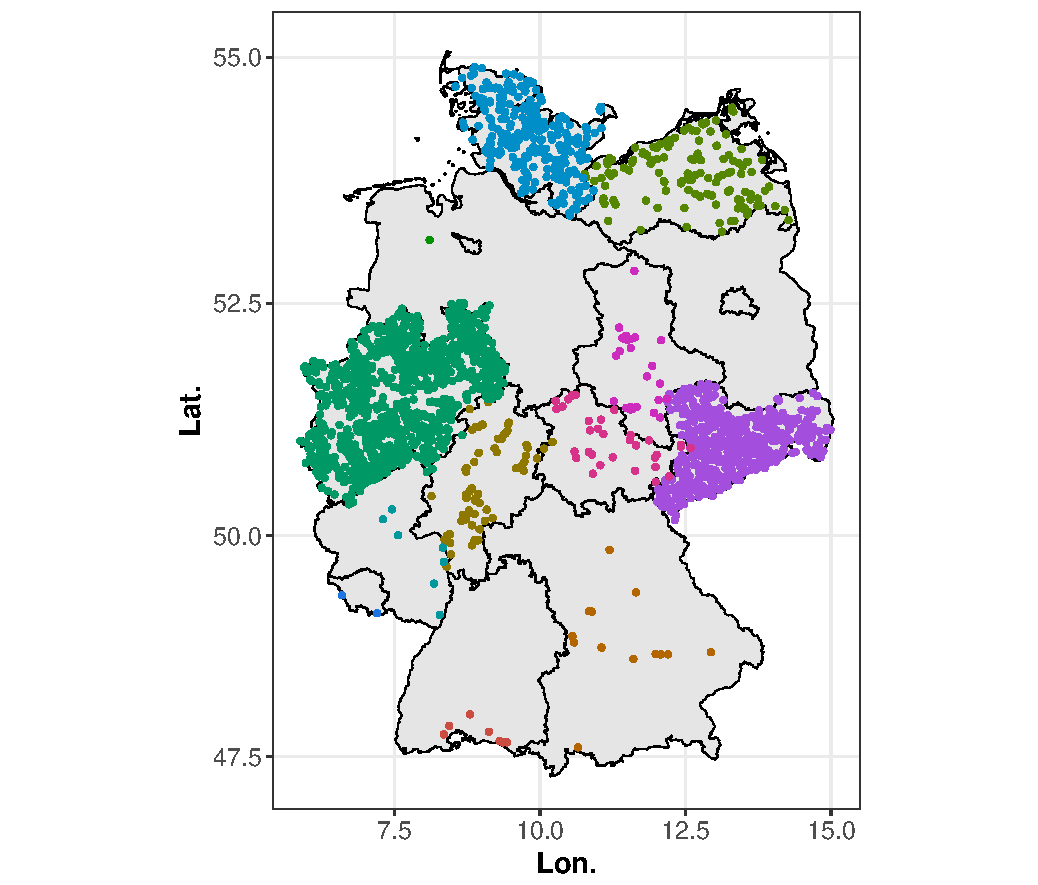
\includegraphics[width = 1.4\textwidth]{figs/map_phch.pdf}
	 \end{columns}
\end{frame}


\begin{frame}
\frametitle{Monitoring: Small streams are underrepresented}
	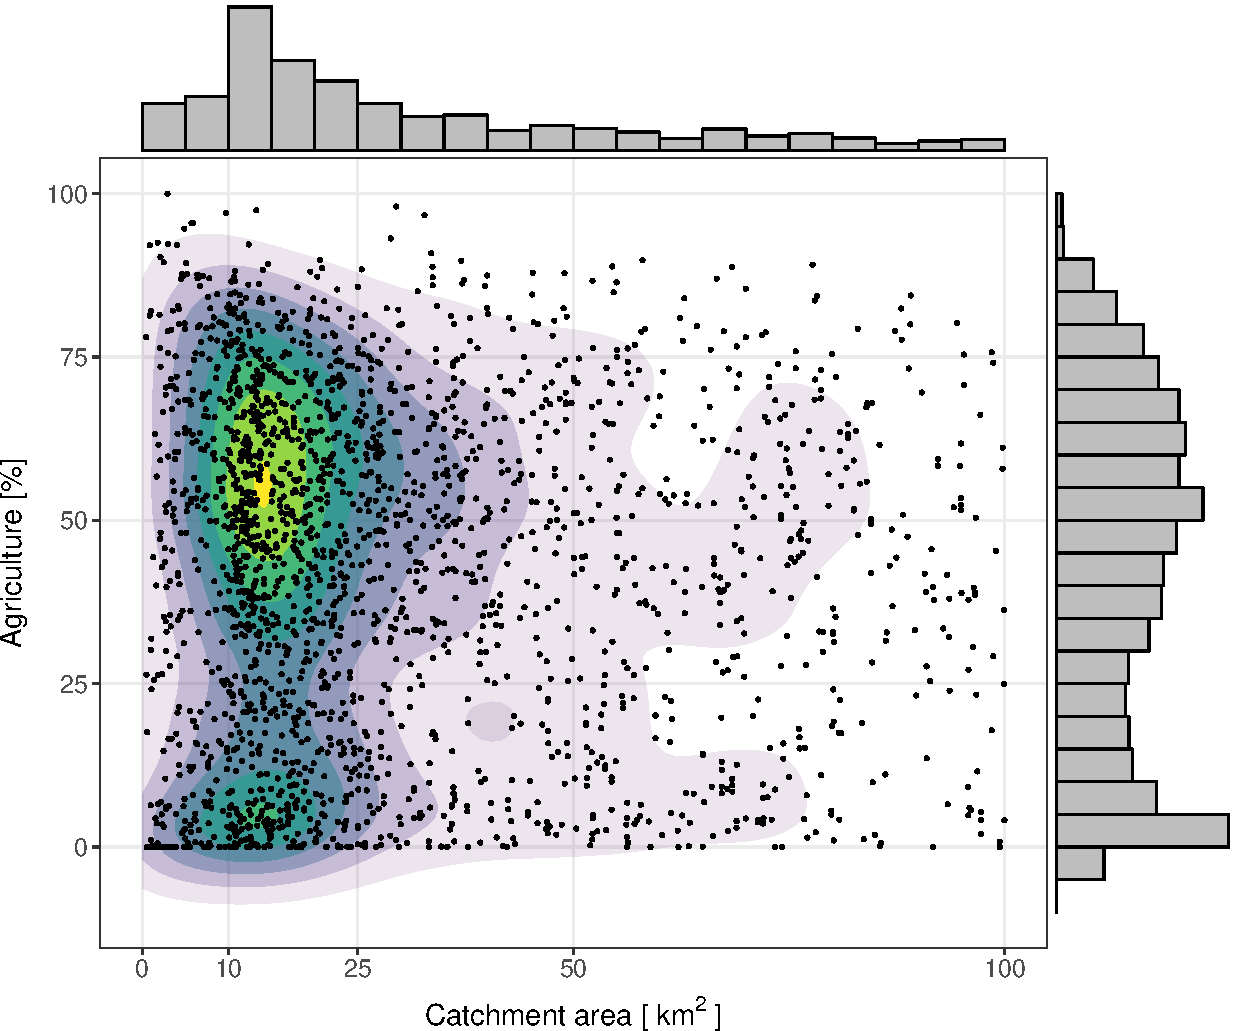
\includegraphics[width = 0.85\textwidth]{figs/distribution.pdf}
\end{frame}


\begin{frame}
\frametitle{Landscape: Factors influencing risk}
	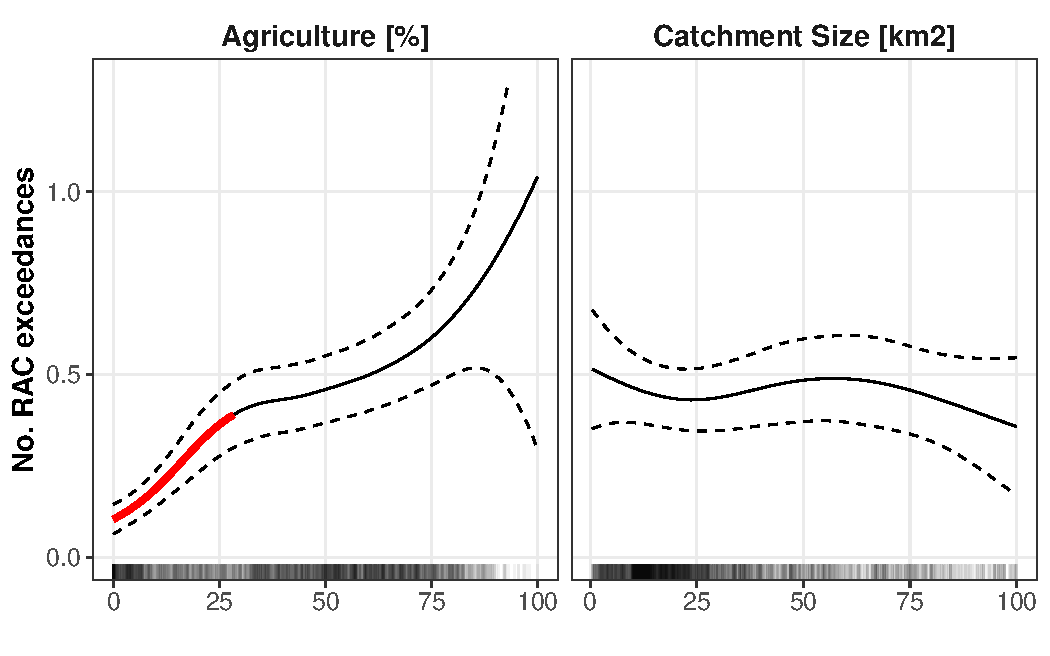
\includegraphics[width = 1\textwidth]{figs/agri_size_eff.pdf}
\end{frame}


\begin{frame}
\frametitle{Sampling: Factors influencing risk}
	\begin{columns}
	    \column{.49\textwidth}
			\resizebox{1.2\textwidth}{!}{%
				\begingroup
				\footnotesize % = 10pt in 12pt default
					\hspace*{-10mm}% Created by tikzDevice version 0.10.1 on 2017-01-09 11:23:21
% !TEX encoding = UTF-8 Unicode
\begin{tikzpicture}[x=1pt,y=1pt]
\definecolor{fillColor}{RGB}{255,255,255}
\path[use as bounding box,fill=fillColor,fill opacity=0.00] (0,0) rectangle (433.62,409.53);
\begin{scope}
\path[clip] (  0.00,  0.00) rectangle (433.62,409.53);
\definecolor{drawColor}{RGB}{255,255,255}
\definecolor{fillColor}{RGB}{255,255,255}

\path[draw=drawColor,line width= 0.6pt,line join=round,line cap=round,fill=fillColor] (  0.00,  0.00) rectangle (433.62,409.53);
\end{scope}
\begin{scope}
\path[clip] ( 61.28, 52.71) rectangle (424.62,351.71);
\definecolor{fillColor}{RGB}{255,255,255}

\path[fill=fillColor] ( 61.28, 52.71) rectangle (424.62,351.71);
\definecolor{drawColor}{gray}{0.90}

\path[draw=drawColor,line width= 0.6pt,line join=round] ( 61.28, 59.17) --
	(424.62, 59.17);

\path[draw=drawColor,line width= 0.6pt,line join=round] ( 61.28,131.95) --
	(424.62,131.95);

\path[draw=drawColor,line width= 0.6pt,line join=round] ( 61.28,204.74) --
	(424.62,204.74);

\path[draw=drawColor,line width= 0.6pt,line join=round] ( 61.28,277.52) --
	(424.62,277.52);

\path[draw=drawColor,line width= 0.6pt,line join=round] ( 61.28,350.30) --
	(424.62,350.30);

\path[draw=drawColor,line width= 0.6pt,line join=round] (372.71, 52.71) --
	(372.71,351.71);

\path[draw=drawColor,line width= 0.6pt,line join=round] (286.20, 52.71) --
	(286.20,351.71);

\path[draw=drawColor,line width= 0.6pt,line join=round] (199.69, 52.71) --
	(199.69,351.71);

\path[draw=drawColor,line width= 0.6pt,line join=round] (113.18, 52.71) --
	(113.18,351.71);
\definecolor{drawColor}{RGB}{0,0,0}

\path[draw=drawColor,line width= 1.1pt,line join=round] (113.18, 66.30) -- (113.18,142.59);

\path[draw=drawColor,line width= 1.1pt,line join=round] (199.69,172.78) -- (199.69,338.12);

\path[draw=drawColor,line width= 1.1pt,line join=round] (286.20,131.27) -- (286.20,292.39);

\path[draw=drawColor,line width= 1.1pt,line join=round] (372.71, 97.61) -- (372.71,230.40);
\definecolor{fillColor}{RGB}{0,0,0}

\path[draw=drawColor,line width= 0.8pt,line join=round,line cap=round,fill=fillColor] (113.18, 98.42) circle (  5.00);

\path[draw=drawColor,line width= 0.8pt,line join=round,line cap=round,fill=fillColor] (199.69,243.98) circle (  5.00);

\path[draw=drawColor,line width= 0.8pt,line join=round,line cap=round,fill=fillColor] (286.20,198.37) circle (  5.00);

\path[draw=drawColor,line width= 0.8pt,line join=round,line cap=round,fill=fillColor] (372.71,152.08) circle (  5.00);
\definecolor{drawColor}{RGB}{216,130,27}
\definecolor{fillColor}{RGB}{216,130,27}

\path[draw=drawColor,line width= 0.4pt,line join=round,line cap=round,fill=fillColor] (113.18,138.08) circle (  4.64);

\path[draw=drawColor,line width= 0.4pt,line join=round,line cap=round,fill=fillColor] (199.69,327.57) circle (  4.64);

\path[draw=drawColor,line width= 0.4pt,line join=round,line cap=round,fill=fillColor] (286.20,269.09) circle (  4.64);

\path[draw=drawColor,line width= 0.4pt,line join=round,line cap=round,fill=fillColor] (372.71,208.90) circle (  4.64);
\definecolor{drawColor}{gray}{0.50}

\path[draw=drawColor,line width= 0.6pt,line join=round,line cap=round] ( 61.28, 52.71) rectangle (424.62,351.71);
\end{scope}
\begin{scope}
\path[clip] (  0.00,  0.00) rectangle (433.62,409.53);
\definecolor{drawColor}{gray}{0.30}

\node[text=drawColor,anchor=base east,inner sep=0pt, outer sep=0pt, scale=  1.44] at ( 53.18, 49.23) {\bfseries 3};

\node[text=drawColor,anchor=base east,inner sep=0pt, outer sep=0pt, scale=  1.44] at ( 53.18,122.02) {\bfseries 6};

\node[text=drawColor,anchor=base east,inner sep=0pt, outer sep=0pt, scale=  1.44] at ( 53.18,194.80) {\bfseries 9};

\node[text=drawColor,anchor=base east,inner sep=0pt, outer sep=0pt, scale=  1.44] at ( 53.18,267.58) {\bfseries 12};

\node[text=drawColor,anchor=base east,inner sep=0pt, outer sep=0pt, scale=  1.44] at ( 53.18,340.36) {\bfseries 15};
\end{scope}
\begin{scope}
\path[clip] (  0.00,  0.00) rectangle (433.62,409.53);
\definecolor{drawColor}{RGB}{0,0,0}

\path[draw=drawColor,line width= 0.6pt,line join=round] ( 56.78, 59.17) --
	( 61.28, 59.17);

\path[draw=drawColor,line width= 0.6pt,line join=round] ( 56.78,131.95) --
	( 61.28,131.95);

\path[draw=drawColor,line width= 0.6pt,line join=round] ( 56.78,204.74) --
	( 61.28,204.74);

\path[draw=drawColor,line width= 0.6pt,line join=round] ( 56.78,277.52) --
	( 61.28,277.52);

\path[draw=drawColor,line width= 0.6pt,line join=round] ( 56.78,350.30) --
	( 61.28,350.30);
\end{scope}
\begin{scope}
\path[clip] (  0.00,  0.00) rectangle (433.62,409.53);
\definecolor{drawColor}{RGB}{0,0,0}

\path[draw=drawColor,line width= 0.6pt,line join=round] (372.71, 48.21) --
	(372.71, 52.71);

\path[draw=drawColor,line width= 0.6pt,line join=round] (286.20, 48.21) --
	(286.20, 52.71);

\path[draw=drawColor,line width= 0.6pt,line join=round] (199.69, 48.21) --
	(199.69, 52.71);

\path[draw=drawColor,line width= 0.6pt,line join=round] (113.18, 48.21) --
	(113.18, 52.71);
\end{scope}
\begin{scope}
\path[clip] (  0.00,  0.00) rectangle (433.62,409.53);
\definecolor{drawColor}{gray}{0.30}

\node[text=drawColor,anchor=base,inner sep=0pt, outer sep=0pt, scale=  1.44] at (372.71, 34.68) {\bfseries Oct-Dec};

\node[text=drawColor,anchor=base,inner sep=0pt, outer sep=0pt, scale=  1.44] at (286.20, 34.68) {\bfseries Jul-Sep};

\node[text=drawColor,anchor=base,inner sep=0pt, outer sep=0pt, scale=  1.44] at (199.69, 34.68) {\bfseries Apr-Jun};

\node[text=drawColor,anchor=base,inner sep=0pt, outer sep=0pt, scale=  1.44] at (113.18, 34.68) {\bfseries Jan-Mar};
\end{scope}
\begin{scope}
\path[clip] (  0.00,  0.00) rectangle (433.62,409.53);
\definecolor{drawColor}{RGB}{0,0,0}

\node[text=drawColor,rotate= 90.00,anchor=base,inner sep=0pt, outer sep=0pt, scale=  2.16] at ( 28.45,202.21) {Percent exceeed LOQ};
\end{scope}
\begin{scope}
\path[clip] (  0.00,  0.00) rectangle (433.62,409.53);
\definecolor{drawColor}{RGB}{0,0,0}

\node[text=drawColor,anchor=base west,inner sep=0pt, outer sep=0pt, scale=  1.62] at ( 61.28,361.75) {n = 23 compounds, orange: 15mm precipitation.};
\end{scope}
\begin{scope}
\path[clip] (  0.00,  0.00) rectangle (433.62,409.53);
\definecolor{drawColor}{RGB}{0,0,0}

\node[text=drawColor,anchor=base west,inner sep=0pt, outer sep=0pt, scale=  2.16] at ( 61.28,385.65) {Annual pattern of detects};
\end{scope}
\end{tikzpicture}

				\endgroup
				}

	    \column{.51\textwidth}
	    	\begin{itemize}
	    		\item Peak in summer
	    		\item Increase by \alert{precipitation}
	    		\item absolute concentrations \textgreater\textgreater variability
	    	\end{itemize}
	\end{columns}
\end{frame}



\begin{frame}
\frametitle{Risks: Compounds exceeding risk thresholds}
    \begin{itemize}
		\item 25\% of sites with at least one RQ > 1
	\end{itemize}
	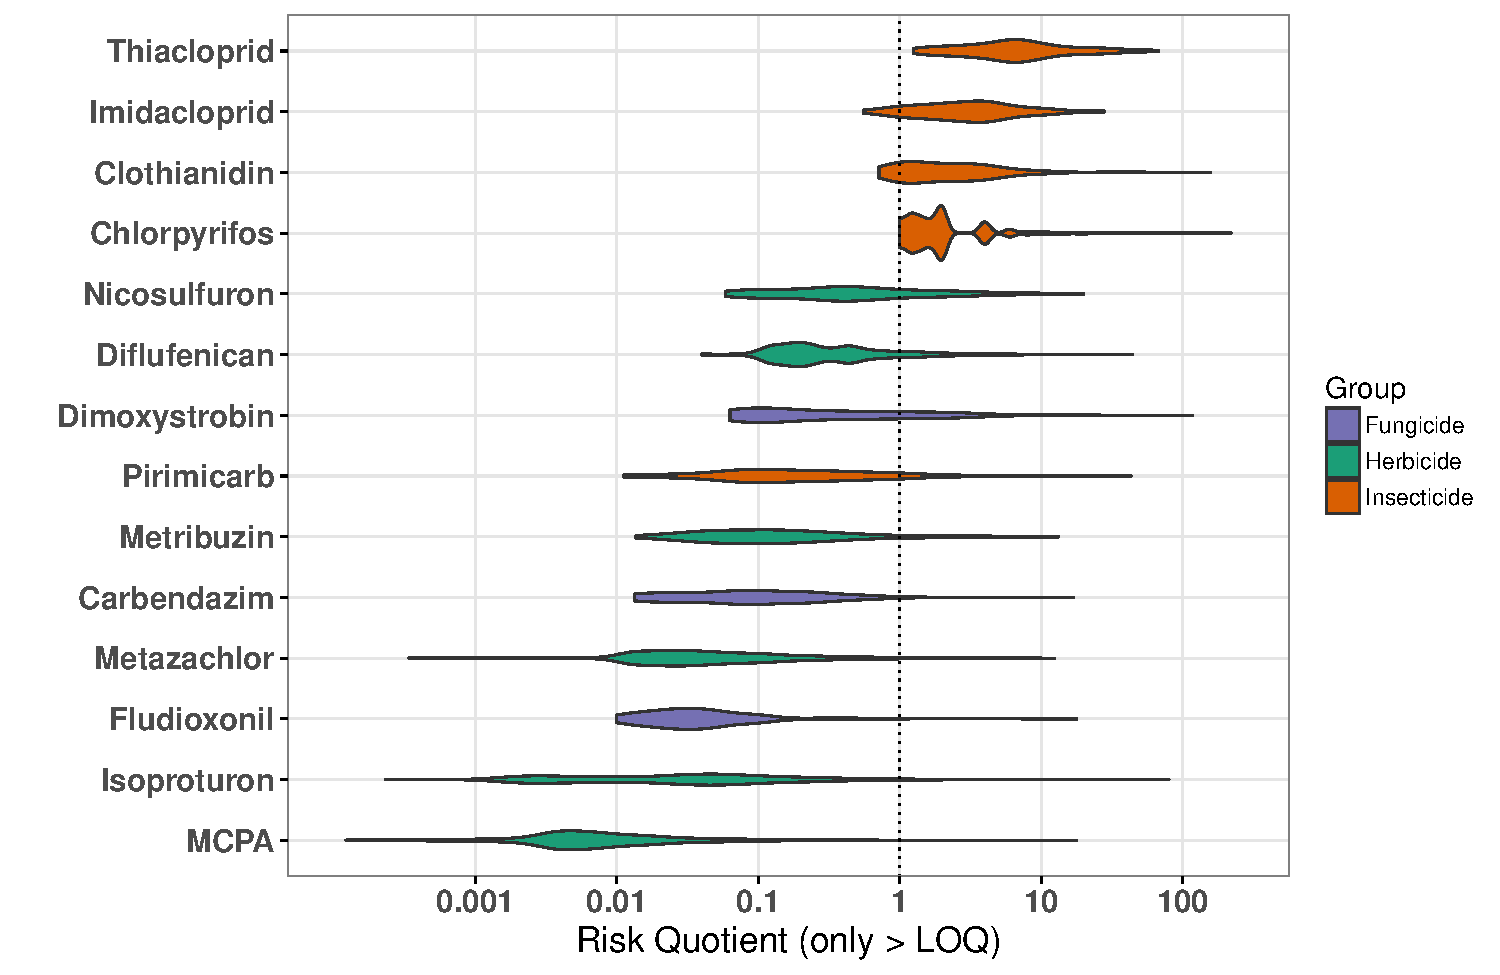
\includegraphics[width = 1\textwidth]{figs/compounds.pdf}
\end{frame}


\begin{frame}
\frametitle{What we learned from this study}
	\begin{enumerate}
		\item Differences between \alert{states}
		\item Small streams are \alert{underrepresented}
		\item \alert{Agricultural} sources
		\item \alert{LOQ} gives additional insights
			\begin{itemize}
				\item Annual \alert{dynamics}
				\item \alert{Precipitation} increases concentrations
			\end{itemize}
		\item Currently \alert{Neonicotinoids} pose a risk
	\end{enumerate}
\end{frame}



%%% ---------------------------------------------------------------------------
\section{Solutions for Data Handling}

\begingroup
\footnotesize % = 10pt in 12pt default
\begin{frame}[noframenumbering]
\frametitle{Solutions for Data Handling in ERA}
    \vspace*{0mm}
	\resizebox{1.02\textwidth}{!}{
		\hspace*{-20mm}% -*- root: ../../talk.tex -*-

% Define elements
% arrows, see also http://tex.stackexchange.com/questions/5461/is-it-possible-to-change-the-size-of-an-arrowhead-in-tikz-pgf/161238#161238
\tikzstyle{line} = [draw, -{Latex[length=4mm,width=3mm]}, ultra thick]
% rectangles
\tikzstyle{block} = [rectangle, draw, 
    text width=5em, text centered, rounded corners, minimum height=4em]
% papers
\tikzstyle{paper} = [circle, draw, fill=myalert,  font = \bf\LARGE, minimum width=1.5cm]
\tikzstyle{textbf} = [text centered, font = \bf\large]

% http://tex.stackexchange.com/questions/55806/mindmap-tikzpicture-in-beamer-reveal-step-by-step/55849#55849
% overlays etc in tikz
\tikzset{
    invisible/.style={opacity=0},
    visible on/.style={alt={#1{}{invisible}}},
    alt/.code args={<#1>#2#3}{%
      \alt<#1>{\pgfkeysalso{#2}}{\pgfkeysalso{#3}} % \pgfkeysalso doesn't change the path
    },
  }

 \definecolor{ao}{rgb}{0.00, 0.40, 0.60}
% \usetikzlibrary{shapes, arrows, positioning, calc, arrows.meta, snakes}
% \definecolor{myalert}{rgb}{0.922, 0.482, 0.078}


\begin{tikzpicture}[node distance = 2cm, auto]
	
% clip figure
\clip(-1.5, -11.5) rectangle (21.0, 4);

% % % grid for coordinates for clip
\draw[help lines,xstep=1,ystep=1] (-2,-13) grid (30,6.5);
\foreach \x in {-2,-1,...,30} { \node [anchor=north] at (\x,0) {\x}; }
\foreach \y in {-13,-12,...,6} { \node [anchor=east] at (0,\y) {\y}; }


% Nodes
	%% Effects
	\node [name = exp, block, minimum width=2cm] {Experiment} ;
	\node [name = stat, block, minimum width=2cm, right=1cm of exp] {Data / Statistics} ;
    \node [name = eff, block, 
		minimum width=57mm, 
		minimum height=25mm, 
		below left=5mm of exp.west, anchor = west] {} ;
	\node[textbf, below right=8mm and 5mm of exp, anchor = south]{Effects};

	%% Exposure
  	\node [name = prop, block, minimum width=2cm, below=38mm of exp] {Data / Properties} ;
	\node [name = model, block, minimum width=2cm, right=1cm of prop] {Models} ;
	\node [name = expo, block, 
		minimum width=57mm, 
		minimum height=25mm, 
		below = 20mm of eff] {} ;
	\node[textbf, above=-2mm of expo, anchor = north]{Exposure};

	%% Monitoring data
	\node [name = monit, block, 
		right = 7.5cm of risk,
        minimum width=35mm, 
		minimum height=20mm, 
		font = \bf\large,
		align = center,
        text width = 3.5cm,
        visible on=<1->] {Environmental\\ Monitoring};


	%% Risk Assessment
	\node [name = risk, block, below right=0.6cm and 1cm of stat,
       minimum width=45mm, 
		minimum height=2.5cm, 
		font = \bf\large,
		align = center,
       text width = 3cm,
       visible on=<1->] {Environmental Risk\\  Assessment};

	%% biological data
	\node [name = bio, block, 
		above left = 2cm and 2cm of monit, anchor = north,
		minimum width=30mm, align = center, text width = 30mm, font=\large] {Biology   };
	%% chemical data
	\node [name = chem, block, 
		below left = 2cm and 2cm of monit, anchor = south,
		minimum width=3cm, font=\large,text width = 30mm] { Chemistry};

	%% Legislation
   \node[name=dir, above= 10mm of eff, font=\large, text width = 60mm, fill = ao, text=white, xshift=10mm,
   visible on=<1->]{\textbf{Plant Protection Products Regulation 1107/2009}};
   \node[name=wfd, right= 80mm of dir, font=\large, text width = 65mm, 
   fill = ao, text=white,
   visible on=<1->]{\textbf{Water Framework Directive 2000/60/EC}};


  %% Papers
  	\node[name = chap2, paper, 
		above left = 5mm and -15mm of stat, 
		anchor = east, fill=lightgray]{1};	
    \node[name = chap3, paper, 
		below left = -22mm and 0mm of chem, anchor = north, fill=lightgray
		]{2};

	\node[name = chap4, paper, anchor = north, yshift=-25mm,  xshift = 10mm] (chap4) at ($(chem)!0.5!(expo)$) {3};
	\node[name = chap5, paper, anchor = south, yshift=20mm, xshift = 10mm] (chap5) at ($(bio)!0.5!(eff)$) {4};

	\node[name = chap4a, paper, 
		below = 35mm of expo, 
		anchor = east]{3};	
	\node[name = chap4t, right = 5mm of chap4a, font = \bf\normalsize, color = myalert, text width = 200mm]{Szöcs \& Schäfer (accepted). “webchem: An R Package to Retrieve Chemical Information from the Web”. Journal of Statistical Software.};

	\node[name = chap5a, paper, 
		below = -3mm of chap4a]{4};	
	\node[name = chap5t, right = 5mm of chap5a, font = \bf\normalsize, color = myalert, text width = 200mm]{Chamberlain \& Szöcs (2013). “taxize: taxonomic search and retrieval in R”. F1000Research 2(191).};
	

% arrows
	\path [line] (prop) -- (model);
		\path [line] (expo) -| node[pos = 0.4, font = \large,  below]{PEC} (risk);
		\path [line] (exp) -- (stat);
	\path [line] (eff) -| node[pos = 0.4, font = \large]{RAC} (risk);
	\path [line] (monit) |- (bio);
	\path [line] (monit) |- (chem);
	\path [dashed,
	visible on=<1->] (risk.south east) edge [line ,bend right = 40]  node [xshift = -4mm, yshift = -7mm, pos =0.1, below, font = \large, align = center] {Approves \\ Substance} (chem);
	\path [dashed] ([yshift=5mm]bio.south west) edge[line, bend left = -10]   ([yshift=0mm]risk.north east);
    \path [dashed] (chap3.north west) edge [line, bend right = 30] node[xshift = 20mm, yshift =11mm, font = \large, align = center] {Retrospection}  (risk);
    \path [line, dashed] (chap4) edge [bend left = 15, color=myalert]  (prop);
    \path [line, dashed] (chap5) edge [bend right = 15, color=myalert]   (stat);
	\path [line, dashed] (chap4) edge [bend right = 15, color=myalert]   (chem);
    \path [line, dashed] (chap5) edge [bend left = 15, color=myalert]   (bio);

    \node[name=rl1, above= 0mm of chap4, font=\large, color=myalert]{Retrieve \& Link data};
     \node[name=rl1, above= 0mm of chap5, font=\large, color=myalert]{Retrieve \& Link data};

\end{tikzpicture}

	}
\end{frame}
\endgroup

% {\setbeamertemplate{frame footer}{Ziemann, M., Eren, Y., El-Osta, A., 2016. Gene name errors are widespread in the scientific literature. Genome Biology 17. 
% }
\begin{frame}
\frametitle{Biologists \& Chemists face the same problems}
	\small
	\centering
	\pause
	\textbf{\alert{\underline{Names}}}
	\begin{columns}[t]
	\column{.45\textwidth}
	\emph{Osmia rufa, Osmia bicornis, Osmia ruffa, Osmiaxuxx} 
	\column{.45\textwidth}
	Chlorpyrifos, Chlorpyriphos, Chlorphyrifos, Chlorpypixx
	\end{columns}
	\pause

	\centering
	\textbf{\alert{\underline{Hierarchies}}}
	\begin{columns}[t]
	\column{.45\textwidth}
	Hymenoptera/ Apoidea/ Megachilidae/ Osmia/ rufa 
	\column{.45\textwidth}
	organophospate, ester, insecticide
	\end{columns}
	\pause

	\centering
	\textbf{\alert{\underline{Traits / Properties}}}
	\begin{columns}[t]
	\column{.45\textwidth}
	Wing length, Mass, Season 
	\column{.45\textwidth}
	Mass, $K_{OW}$, $LC_{50}$
	\end{columns}
	\pause

	\centering
	\textbf{\alert{\underline{Identifiers}}}
	\begin{columns}[t]
	\column{.45\textwidth}
	NCBI, ITIS, EOL, ... 
	\column{.45\textwidth}
	2921-88-2, SMILES, InChI, ...
	\end{columns}
	% \vspace{0.5em}
	\pause

	\rule{\textwidth}{1pt}
	\textbf{\alert{\underline{Amount of data}}}

	\begin{columns}[t]
	\column{.45\textwidth}
	\centering
	\textasciitilde 3000 taxa
	\column{.45\textwidth}
	\centering
	\textasciitilde 500 pesticides
	\end{columns}
\end{frame}
% }




\begin{frame}{}
\frametitle{Instead of wasting time...}
... use \alert{\textbf{webchem}}! \\	
	\vspace*{-0.6cm}
	\hspace*{2cm}
		\begin{adjustbox}{max totalsize={1.1\textwidth}{0.9\textheight}}
		\begingroup
		\footnotesize % = 10pt in 12pt default
					% -*- root: ../../talk.tex -*-

\definecolor{blue}{RGB}{32, 126, 153}
\definecolor{green}{RGB}{33, 182, 78}
\definecolor{red}{RGB}{246, 72, 45}
\definecolor{orange}{RGB}{246, 146, 45}
\definecolor{yellow}{RGB}{180, 180, 18}

\begin{tikzpicture}[node distance = 0.2cm, auto]

%styles
\tikzstyle{circ} = [circle, draw, text = black,   line width=1pt, 
    text width=4cm, text centered, scale=1, font=\bf\huge]
\tikzstyle{rect} = [rectangle, draw, text = black, line width=1pt,
    text width=5cm, text centered, rounded corners, minimum height=1.5cm, minimum width=1cm, font=\bf\huge]

\tikzstyle{line} = [draw, -{Latex[length=5mm,width=3mm]}, line width=1mm, opacity = 0.8]

    % input nodes
    \node [circ, fill=green] (cas_i) {CAS};
    \node  (name_i) [circ, below=of cas_i, fill = blue] {Name};
    \node  (inchikey_i) [circ, below=of name_i, fill = red] {InChiKey};
    \node  (other_i) [circ, below=of inchikey_i, fill =orange] {Other};
   
   % source nodes
   \node (cir) [rect, right=of cas_i, shift={(13,7)}, fill = yellow]{CIR};
   \node (chemspider) [rect, below=1cm of cir, fill = yellow]{ChemSpider};
   \node (cts) [rect, below=1cm of chemspider, fill = yellow]{CTS};
   \node (etox) [rect, below=1cm of cts, fill = yellow]{ETOX};
   \node (chemid) [rect, below=1cm of etox, fill = yellow]{ChemID};
  \node (opsin) [rect, below=1cm of chemid, fill = yellow]{OPSIN};
  \node (alan) [rect, below=1cm of opsin, fill = yellow]{Pesticide Compendium};
  \node (wiki) [rect, below=1cm of alan, fill = yellow]{wikidata};
  \node (pubchem) [rect, below=1cm of wiki, fill = yellow]{PubChem};
  \node (pan) [rect, below=1cm of pubchem, fill = yellow]{PAN};
  \node (src) [rect, below=1cm of pan, fill = yellow]{SRC};

	% output nodes
    \node (cas_o) [circ, right=of cir, shift={(15,-5)}, , fill =green] {CAS};
    \node  (name_o) [circ, below=of cas_o, , fill =blue] {Name};
    \node  (inchikey_o) [circ, below=of name_o, fill =red] {InChiKey \\ InChi};
    \node  (smiles_o) [circ, below=of inchikey_o, fill =red] {SMILES};
    \node  (legis_o) [circ, below=of smiles_o, fill =orange] {Legislation};
    \node  (syno_o) [circ, below=of legis_o, fill =orange] {Synonyms};
    \node  (other_o) [circ, below=of syno_o, fill =orange] {Other};
    \node (prop_o) [circ, above=of cas_o, fill =orange] {Properties};
    \node (tox_o) [circ, above=of prop_o, fill =orange] {Toxicology};

    %paths
   % from cas_i
    \path [line, green] (cas_i.east) -- (cir.west);
    \path [line, green] (cas_i.east) -- (chemspider.west);
    \path [line, green] (cas_i.east) -- (cts.west);
    \path [line, green] (cas_i.east) -- (etox.west);
    \path [line, green] (cas_i.east) -- (chemid.west);
    \path [line, green] (cas_i.east) -- (alan.west);
    \path [line, green] (cas_i.east) -- (wiki.west);
    \path [line, green] (cas_i.east) -- (pubchem.west);
    \path [line, green] (cas_i.east) -- (pan.west);
    \path [line, green] (cas_i.east) -- (src.west);

	% from name_i
    \path [line, blue] (name_i.east) -- (cir.west);
    \path [line, blue] (name_i.east) -- (chemspider.west);
    \path [line, blue] (name_i.east) -- (cts.west);
    \path [line, blue] (name_i.east) -- (etox.west);
    \path [line, blue] (name_i.east) -- (chemid.west);
    \path [line, blue] (name_i.east) -- (opsin.west);
    \path [line, blue] (name_i.east) -- (alan.west);
    \path [line, blue] (name_i.east) -- (wiki.west);
    \path [line, blue] (name_i.east) -- (pubchem.west);
    \path [line, blue] (name_i.east) -- (pan.west);

    %from inchikey_i
    \path [line, red] (inchikey_i.east) -- (cir.west);
    \path [line, red] (inchikey_i.east) -- (chemspider.west);
    \path [line, red] (inchikey_i.east) -- (cts.west);
    \path [line, red] (inchikey_i.east) -- (chemid.west);
    \path [line, red] (inchikey_i.east) -- (wiki.west);
    \path [line, red] (inchikey_i.east) -- (pubchem.west);
   
    %from other_i
    \path [line, orange] (other_i.east) -- (cir.west);
    \path [line, orange] (other_i.east) -- (chemspider.west);
    \path [line, orange] (other_i.east) -- (cts.west);
    \path [line, orange] (other_i.east) -- (etox.west);
    \path [line, orange] (other_i.east) -- (wiki.west);
    \path [line, orange] (other_i.east) -- (pubchem.west);

   %from cir
  \path [line, orange] (cir.east) -- (prop_o.west);
  \path [line, green] (cir.east) -- (cas_o.west);
  \path [line, blue] (cir.east) -- (name_o.west);
  \path [line, red] (cir.east) -- (inchikey_o.west);
  \path [line, red] (cir.east) -- (smiles_o.west);
  \path [line, orange] (cir.east) -- (other_o.west);

  %from chemspider
  \path [line, orange] (chemspider.east) -- (prop_o.west);
  \path [line, blue] (chemspider.east) -- (name_o.west);
  \path [line, red] (chemspider.east) -- (inchikey_o.west);
  \path [line, red] (chemspider.east) -- (smiles_o.west);

  % from cts
  \path [line, blue] (cts.east) -- (name_o.west);
  \path [line, green] (cts.east) -- (cas_o.west);
  \path [line, red] (cts.east) -- (inchikey_o.west);
  \path [line, red] (cts.east) -- (smiles_o.west);
  \path [line, orange] (cts.east) -- (syno_o.west);
  \path [line, orange] (cts.east) -- (other_o.west);

	% from etox
   \path [line, orange] (etox.east) -- (tox_o.west);
   \path [line, green] (etox.east) -- (cas_o.west);
   \path [line, blue] (etox.east) -- (name_o.west);
   \path [line, orange] (etox.east) -- (legis_o.west);
   \path [line, orange] (etox.east) -- (syno_o.west);
   \path [line, orange] (etox.east) -- (other_o.west);

  %from chemid
   \path [line, orange] (chemid.east) -- (tox_o.west);
   \path [line, orange] (chemid.east) -- (prop_o.west);
   \path [line, green] (chemid.east) -- (cas_o.west);
   \path [line, blue] (chemid.east) -- (name_o.west);
   \path [line, red] (chemid.east) -- (inchikey_o.west);
   \path [line, red] (chemid.east) -- (smiles_o.west);
   \path [line, orange] (chemid.east) -- (syno_o.west);

	%from opsin
    \path [line, green] (opsin.east) -- (cas_o.west);
   \path [line, red] (opsin.east) -- (inchikey_o.west);
   \path [line, red] (opsin.east) -- (smiles_o.west);

   %from alan wood
   \path [line, green] (alan.east) -- (cas_o.west);
   \path [line, blue] (alan.east) -- (name_o.west);
   \path [line, red] (alan.east) -- (inchikey_o.west);
   \path [line, orange] (alan.east) -- (other_o.west);

  %from wiki
   \path [line, green] (wiki.east) -- (cas_o.west);
   \path [line, red] (wiki.east) -- (inchikey_o.west);
   \path [line, red] (wiki.east) -- (smiles_o.west);
   \path [line, orange] (wiki.east) -- (other_o.west);

  % from pubchem
     \path [line, orange] (pubchem.east) -- (prop_o.west);
     \path [line, blue] (pubchem.east) -- (name_o.west);
     \path [line, red] (pubchem.east) -- (inchikey_o.west);
     \path [line, red] (pubchem.east) -- (smiles_o.west);
     \path [line, orange] (pubchem.east) -- (syno_o.west);

    % from pan
    \path [line, orange] (pan.east) -- (tox_o.west);
    \path [line, orange] (pan.east) -- (prop_o.west);
     \path [line, blue] (pan.east) -- (name_o.west);
   \path [line, green] (pan.east) -- (cas_o.west);
   \path [line, orange] (pan.east) -- (legis_o.west);
   \path [line, orange] (pan.east) -- (other_o.west);

  %from src
       \path [line, orange] (src.east) -- (tox_o.west);
     \path [line, blue] (src.east) -- (name_o.west);
   \path [line, green] (src.east) -- (cas_o.west);

\end{tikzpicture}

		\endgroup
		\end{adjustbox} \\
	\Put(-20, 375){
		
\includegraphics[width=0.17\textwidth]{figs/Rlogo.png}
	}
\\
\only<2->{
	\begingroup
	\footnotesize
	\vspace*{-1.5cm}\emph{''\alert{\textbf{webchem}} ...likely saved hundreds of working hours''} \\[3mm]
	\endgroup
	\tiny Münch et al. (2016). DoOR 2.0 - Comprehensive Mapping of Drosophila melanogaster Odorant Responses. Scientific Reports 6, 21841
}
\end{frame}



\begin{frame}
\frametitle{Instead of wasting time...}
	... use \alert{\textbf{taxize}}! \\
	\begin{center}
		\hspace*{1.5cm}
\includegraphics[height=0.6\textheight]{figs/sources_taxize.png}
	\end{center}
	\Put(-20, 311){
		
\includegraphics[width=0.17\textwidth]{figs/Rlogo.png}
	}
	\pause
	\Put(20,60){
		\fcolorbox{myalert}{myalert}{
\includegraphics[width=0.7\textwidth]{figs/taxize_twitter.png}}
	}
\end{frame}



% \begin{frame}
% \frametitle{taxize \& webchem: Advances for you (researchers)}
% 	\begin{enumerate}
% 		\item save time % data cleaning takes 80% of resources
% 		\item less errors
% 		\item reproducibility
% 		\item joins
% 		\item aggregations
% 	\end{enumerate}
% \end{frame}


%%% ---------------------------------------------------------------------------
\section*{Recap}

\begingroup
\footnotesize % = 10pt in 12pt default
\begin{frame}
\frametitle{Recap: What did I look at?}
    \vspace*{2mm}
	\resizebox{1.1\textwidth}{!}{
		\hspace*{-20mm}% -*- root: ../../talk.tex -*-

% Define elements
% arrows, see also http://tex.stackexchange.com/questions/5461/is-it-possible-to-change-the-size-of-an-arrowhead-in-tikz-pgf/161238#161238
\tikzstyle{line} = [draw, -{Latex[length=4mm,width=3mm]}, ultra thick]
% rectangles
\tikzstyle{block} = [rectangle, draw, 
    text width=5em, text centered, rounded corners, minimum height=4em]
% papers
\tikzstyle{paper} = [circle, draw, fill=myalert,  font = \bf\LARGE, minimum width=1.5cm]
\tikzstyle{textbf} = [text centered, font = \bf\large]

% http://tex.stackexchange.com/questions/55806/mindmap-tikzpicture-in-beamer-reveal-step-by-step/55849#55849
% overlays etc in tikz
\tikzset{
    invisible/.style={opacity=0},
    visible on/.style={alt={#1{}{invisible}}},
    alt/.code args={<#1>#2#3}{%
      \alt<#1>{\pgfkeysalso{#2}}{\pgfkeysalso{#3}} % \pgfkeysalso doesn't change the path
    },
  }

 \definecolor{ao}{rgb}{0.00, 0.40, 0.60}
% \usetikzlibrary{shapes, arrows, positioning, calc, arrows.meta, snakes}
% \definecolor{myalert}{rgb}{0.922, 0.482, 0.078}


\begin{tikzpicture}[node distance = 2cm, auto]
	
% clip figure
\clip(-1.5,-10) rectangle (21.0, 4.0);

% % % % grid for coordinates for clip
% \draw[help lines,xstep=1,ystep=1] (-2,-13) grid (30,6.5);
% \foreach \x in {-2,-1,...,30} { \node [anchor=north] at (\x,0) {\x}; }
% \foreach \y in {-13,-12,...,6} { \node [anchor=east] at (0,\y) {\y}; }


% Nodes
	%% Effects
	\node [name = exp, block, minimum width=2cm] {Experiment} ;
	\node [name = stat, block, minimum width=2cm, right=1cm of exp] {Data / Statistics} ;
    \node [name = eff, block, 
		minimum width=57mm, 
		minimum height=25mm, 
		below left=5mm of exp.west, anchor = west] {} ;
	\node[textbf, below right=8mm and 5mm of exp, anchor = south]{Effects};

	%% Exposure
  	\node [name = prop, block, minimum width=2cm, below=38mm of exp] {Data / Properties} ;
	\node [name = model, block, minimum width=2cm, right=1cm of prop] {Models} ;
	\node [name = expo, block, 
		minimum width=57mm, 
		minimum height=25mm, 
		below = 20mm of eff] {} ;
	\node[textbf, above=-2mm of expo, anchor = north]{Exposure};

	%% Risk Assessment
	\node [name = risk, block, below right=0.75cm and 1cm of stat,
       minimum width=45mm, 
		minimum height=2.5cm, 
		font = \bf\large,
		align = center,
       text width = 3cm] {Environmental Risk\\  Assessment};

	%% Monitoring data
	\node [name = monit, block, 
		right = 7.5cm of risk,
        minimum width=35mm, 
		minimum height=20mm, 
		font = \bf\large,
		align = center,
        text width = 3.5cm,
        visible on=<1->] {Environmental\\ Monitoring};

	%% biological data
	\node [name = bio, block, 
		above left = 2cm and 2cm of monit, anchor = north,
		minimum width=30mm, align = center, text width = 30mm, font=\large] {Biology   };
	%% chemical data
	\node [name = chem, block, 
		below left = 2cm and 2cm of monit, anchor = south,
		minimum width=3cm, font=\large,text width = 30mm] { Chemistry};

	%% Legislation
   \node[name=dir, above= 10mm of eff, font=\large, text width = 60mm, fill = ao, text=white, xshift=10mm,
   visible on=<1->]{\textbf{Plant Protection Products Regulation 1107/2009}};
   \node[name=wfd, right= 80mm of dir, font=\large, text width = 65mm, 
   fill = ao, text=white,
   visible on=<1->]{\textbf{Water Framework Directive 2000/60/EC}};


  %% Papers
  	\node[name = chap2, paper, 
		above left = 5mm and -15mm of stat, 
		anchor = east, fill=myalert]{1};	
    \node[name = chap3, paper, 
		below left = -22mm and 0mm of chem, anchor = north, fill=myalert
		]{2};

	\node[name = chap4, paper, anchor = north, yshift=-25mm,  xshift = 10mm, fill=myalert] (chap4) at ($(chem)!0.5!(expo)$) {3};
	\node[name = chap5, paper, anchor = south, yshift=20mm, xshift = 10mm, fill=myalert] (chap5) at ($(bio)!0.5!(eff)$) {4};

	

% arrows
	\path [line] (prop) -- (model);
		\path [line] (expo) -| node[pos = 0.4, font = \large,  below]{PEC} (risk);
		\path [line] (exp) -- (stat);
	\path [line] (eff) -| node[pos = 0.4, font = \large]{RAC} (risk);
	\path [line] (monit) |- (bio);
	\path [line] (monit) |- (chem);
	\path [dashed,
	visible on=<1->] (risk.south east) edge [line ,bend right = 40]  node [xshift = -4mm, yshift = -7mm, pos =0.1, below, font = \large, align = center] {Approves \\ Substance} (chem);
	\path [dashed] ([yshift=5mm]bio.south west) edge[line, bend left = -10]   ([yshift=0mm]risk.north east);
    \path [dashed] (chap3.north west) edge [line, bend right = 30] node[xshift = 20mm, yshift =11mm, font = \large, align = center] {Retrospection}  (risk);
    \path [line, dashed] (chap4) edge [bend left = 15]  (prop);
    \path [line, dashed] (chap5) edge [bend right = 15]   (stat);
	\path [line, dashed] (chap4) edge [bend right = 15]   (chem);
    \path [line, dashed] (chap5) edge [bend left = 15]   (bio);

    \node[name=rl1, below= 0mm of chap4, font=\large]{Retrieve \& Link data};
     \node[name=rl1, above= 0mm of chap5, font=\large]{Retrieve \& Link data};

\end{tikzpicture}

	}
\end{frame}
\endgroup

\begin{frame}
\frametitle{Recap: What we learned from my PhD Thesis}
	\metroset{block=fill}
	\begin{exampleblock}{\checkmark Improving Statistics in ERA}
		\begin{itemize}
			\item Change your model, not your data
			\item Take LOQ into account
		\end{itemize}
	\end{exampleblock}

\pause
	\begin{exampleblock}{\checkmark~Identifying Risks using Monitoring data}
		\begin{itemize}
			\item Risk drivers and dynamics
			\item Agricultural small streams neglected \& at risk
			\item Currently Neonicotinoids pose a risk
		\end{itemize}
	\end{exampleblock}

\pause
	\begin{exampleblock}{\checkmark Solutions for Data Handling}
		\begin{itemize}
			\item Handling big eco(toxico-)logical data not easy
			\item Now easier
		\end{itemize}
	\end{exampleblock}
\end{frame}



%%% ---------------------------------------------------------------------------
%%% Final slide

\begin{frame}[standout]
	\frametitle{}

	\vspace{1em}
	\Huge{Statistical Ecotoxicology} \\[0.3em]
	\normalsize{Improving the Utilisation of Data for \\ Environmental Risk Assessment} \\[1em]

	\footnotesize
	Eduard Szöcs \\[3em]
\begin{flushleft}
	\faLaptop~~~\textbf{\href{http://edild.github.io}{edild.github.io }}\\[.5em]
	\faTwitter~~~\textbf{\href{http://twitter.com/EduardSzoecs}{@EduardSzoecs}} 	\\[0.5em]
	\faFilePowerpointO~~~\textbf{\href{https://github.com/edild/phd_defense}{github.com/edild/phd\_defense}}\\[0.5em]
	\faBook~~~\textbf{\href{https://github.com/edild/phd_thesis}{github.com/edild/phd\_thesis}}\\[3em]
\end{flushleft}

	\begin{center}\ccbysa\end{center} 
\end{frame}




\appendix

\begin{frame}
\frametitle{Power en detail}
	\begin{adjustbox}{max totalsize={\textwidth}{\textheight}}
				% Created by tikzDevice version 0.10.1 on 2016-12-15 15:38:57
% !TEX encoding = UTF-8 Unicode
\begin{tikzpicture}[x=1pt,y=1pt]
\definecolor{fillColor}{RGB}{255,255,255}
\path[use as bounding box,fill=fillColor,fill opacity=0.00] (0,0) rectangle (1011.78,722.70);
\begin{scope}
\path[clip] (  3.50,423.03) rectangle (1011.78,722.70);
\definecolor{drawColor}{RGB}{255,255,255}
\definecolor{fillColor}{RGB}{255,255,255}

\path[draw=drawColor,line width= 0.6pt,line join=round,line cap=round,fill=fillColor] (  3.50,423.03) rectangle (1011.78,722.70);
\end{scope}
\begin{scope}
\path[clip] ( 66.13,444.26) rectangle (374.35,689.45);
\definecolor{fillColor}{RGB}{255,255,255}

\path[fill=fillColor] ( 66.13,444.26) rectangle (374.35,689.45);
\definecolor{drawColor}{gray}{0.90}

\path[draw=drawColor,line width= 0.6pt,line join=round] ( 66.13,450.69) --
	(374.35,450.69);

\path[draw=drawColor,line width= 0.6pt,line join=round] ( 66.13,530.26) --
	(374.35,530.26);

\path[draw=drawColor,line width= 0.6pt,line join=round] ( 66.13,564.52) --
	(374.35,564.52);

\path[draw=drawColor,line width= 0.6pt,line join=round] ( 66.13,598.79) --
	(374.35,598.79);

\path[draw=drawColor,line width= 0.6pt,line join=round] ( 66.13,633.06) --
	(374.35,633.06);

\path[draw=drawColor,line width= 0.6pt,line join=round] ( 66.13,653.10) --
	(374.35,653.10);

\path[draw=drawColor,line width= 0.6pt,line join=round] ( 66.13,667.32) --
	(374.35,667.32);

\path[draw=drawColor,line width= 0.6pt,line join=round] ( 66.13,678.35) --
	(374.35,678.35);

\path[draw=drawColor,line width= 0.6pt,line join=round] ( 80.14,444.26) --
	( 80.14,689.45);

\path[draw=drawColor,line width= 0.6pt,line join=round] (126.84,444.26) --
	(126.84,689.45);

\path[draw=drawColor,line width= 0.6pt,line join=round] (173.54,444.26) --
	(173.54,689.45);

\path[draw=drawColor,line width= 0.6pt,line join=round] (220.24,444.26) --
	(220.24,689.45);

\path[draw=drawColor,line width= 0.6pt,line join=round] (266.94,444.26) --
	(266.94,689.45);

\path[draw=drawColor,line width= 0.6pt,line join=round] (313.64,444.26) --
	(313.64,689.45);

\path[draw=drawColor,line width= 0.6pt,line join=round] (360.34,444.26) --
	(360.34,689.45);
\definecolor{drawColor}{RGB}{0,0,0}

\path[draw=drawColor,line width= 0.6pt,line join=round] ( 80.14,543.98) --
	(126.84,527.20) --
	(173.54,519.23) --
	(220.24,526.14) --
	(266.94,521.64) --
	(313.64,529.26) --
	(360.34,529.26);

\path[draw=drawColor,line width= 0.6pt,dash pattern=on 2pt off 2pt ,line join=round] ( 80.14,524.93) --
	(126.84,543.29) --
	(173.54,571.78) --
	(220.24,581.39) --
	(266.94,577.49) --
	(313.64,586.51) --
	(360.34,577.54);

\path[draw=drawColor,line width= 0.6pt,dash pattern=on 4pt off 2pt ,line join=round] ( 80.14,545.46) --
	(126.84,532.20) --
	(173.54,531.24) --
	(220.24,534.06) --
	(266.94,516.69) --
	(313.64,531.24) --
	(360.34,534.97);

\path[draw=drawColor,line width= 0.6pt,dash pattern=on 4pt off 4pt ,line join=round] ( 80.14,495.87) --
	(126.84,501.78) --
	(173.54,534.58) --
	(220.24,532.18) --
	(266.94,511.19) --
	(313.64,528.24) --
	(360.34,534.11);

\path[draw=drawColor,line width= 0.6pt,dash pattern=on 1pt off 3pt ,line join=round] ( 80.14,600.97) --
	(126.84,629.07) --
	(173.54,651.76) --
	(220.24,669.62) --
	(266.94,675.19) --
	(313.64,677.71) --
	(360.34,678.30);

\path[draw=drawColor,line width= 0.6pt,dash pattern=on 1pt off 3pt on 4pt off 3pt ,line join=round] ( 80.14,499.80) --
	(126.84,470.74) --
	(173.54,476.93) --
	(220.24,473.93) --
	(266.94,455.41) --
	(313.64,497.93) --
	(360.34,484.96);
\definecolor{fillColor}{RGB}{0,0,0}

\path[fill=fillColor] ( 80.14,543.98) circle (  4.64);

\path[draw=drawColor,line width= 0.4pt,line join=round,line cap=round] ( 80.14,532.14) --
	( 86.39,521.32) --
	( 73.89,521.32) --
	( 80.14,532.14);

\path[draw=drawColor,line width= 0.4pt,line join=round,line cap=round] ( 75.50,540.82) -- ( 84.78,550.10);

\path[draw=drawColor,line width= 0.4pt,line join=round,line cap=round] ( 75.50,550.10) -- ( 84.78,540.82);

\path[draw=drawColor,line width= 0.4pt,line join=round,line cap=round] ( 75.50,491.23) rectangle ( 84.78,500.51);

\path[draw=drawColor,line width= 0.4pt,line join=round,line cap=round] ( 80.14,600.97) circle (  4.64);

\path[fill=fillColor] ( 80.14,507.01) --
	( 86.39,496.19) --
	( 73.89,496.19) --
	cycle;

\path[fill=fillColor] (126.84,527.20) circle (  4.64);

\path[draw=drawColor,line width= 0.4pt,line join=round,line cap=round] (126.84,550.51) --
	(133.09,539.69) --
	(120.59,539.69) --
	(126.84,550.51);

\path[draw=drawColor,line width= 0.4pt,line join=round,line cap=round] (122.20,527.56) -- (131.48,536.84);

\path[draw=drawColor,line width= 0.4pt,line join=round,line cap=round] (122.20,536.84) -- (131.48,527.56);

\path[draw=drawColor,line width= 0.4pt,line join=round,line cap=round] (122.20,497.14) rectangle (131.48,506.42);

\path[draw=drawColor,line width= 0.4pt,line join=round,line cap=round] (126.84,629.07) circle (  4.64);

\path[fill=fillColor] (126.84,477.95) --
	(133.09,467.13) --
	(120.59,467.13) --
	cycle;

\path[fill=fillColor] (173.54,519.23) circle (  4.64);

\path[draw=drawColor,line width= 0.4pt,line join=round,line cap=round] (173.54,579.00) --
	(179.79,568.17) --
	(167.29,568.17) --
	(173.54,579.00);

\path[draw=drawColor,line width= 0.4pt,line join=round,line cap=round] (168.90,526.60) -- (178.18,535.88);

\path[draw=drawColor,line width= 0.4pt,line join=round,line cap=round] (168.90,535.88) -- (178.18,526.60);

\path[draw=drawColor,line width= 0.4pt,line join=round,line cap=round] (168.90,529.94) rectangle (178.18,539.22);

\path[draw=drawColor,line width= 0.4pt,line join=round,line cap=round] (173.54,651.76) circle (  4.64);

\path[fill=fillColor] (173.54,484.14) --
	(179.79,473.32) --
	(167.29,473.32) --
	cycle;

\path[fill=fillColor] (220.24,526.14) circle (  4.64);

\path[draw=drawColor,line width= 0.4pt,line join=round,line cap=round] (220.24,588.61) --
	(226.49,577.79) --
	(213.99,577.79) --
	(220.24,588.61);

\path[draw=drawColor,line width= 0.4pt,line join=round,line cap=round] (215.60,529.42) -- (224.88,538.70);

\path[draw=drawColor,line width= 0.4pt,line join=round,line cap=round] (215.60,538.70) -- (224.88,529.42);

\path[draw=drawColor,line width= 0.4pt,line join=round,line cap=round] (215.60,527.55) rectangle (224.88,536.82);

\path[draw=drawColor,line width= 0.4pt,line join=round,line cap=round] (220.24,669.62) circle (  4.64);

\path[fill=fillColor] (220.24,481.14) --
	(226.49,470.32) --
	(213.99,470.32) --
	cycle;

\path[fill=fillColor] (266.94,521.64) circle (  4.64);

\path[draw=drawColor,line width= 0.4pt,line join=round,line cap=round] (266.94,584.71) --
	(273.19,573.89) --
	(260.69,573.89) --
	(266.94,584.71);

\path[draw=drawColor,line width= 0.4pt,line join=round,line cap=round] (262.30,512.05) -- (271.58,521.33);

\path[draw=drawColor,line width= 0.4pt,line join=round,line cap=round] (262.30,521.33) -- (271.58,512.05);

\path[draw=drawColor,line width= 0.4pt,line join=round,line cap=round] (262.30,506.55) rectangle (271.58,515.83);

\path[draw=drawColor,line width= 0.4pt,line join=round,line cap=round] (266.94,675.19) circle (  4.64);

\path[fill=fillColor] (266.94,462.62) --
	(273.19,451.80) --
	(260.69,451.80) --
	cycle;

\path[fill=fillColor] (313.64,529.26) circle (  4.64);

\path[draw=drawColor,line width= 0.4pt,line join=round,line cap=round] (313.64,593.72) --
	(319.89,582.90) --
	(307.39,582.90) --
	(313.64,593.72);

\path[draw=drawColor,line width= 0.4pt,line join=round,line cap=round] (309.00,526.60) -- (318.28,535.88);

\path[draw=drawColor,line width= 0.4pt,line join=round,line cap=round] (309.00,535.88) -- (318.28,526.60);

\path[draw=drawColor,line width= 0.4pt,line join=round,line cap=round] (309.00,523.60) rectangle (318.28,532.88);

\path[draw=drawColor,line width= 0.4pt,line join=round,line cap=round] (313.64,677.71) circle (  4.64);

\path[fill=fillColor] (313.64,505.15) --
	(319.89,494.32) --
	(307.39,494.32) --
	cycle;

\path[fill=fillColor] (360.34,529.26) circle (  4.64);

\path[draw=drawColor,line width= 0.4pt,line join=round,line cap=round] (360.34,584.76) --
	(366.59,573.94) --
	(354.09,573.94) --
	(360.34,584.76);

\path[draw=drawColor,line width= 0.4pt,line join=round,line cap=round] (355.70,530.33) -- (364.98,539.61);

\path[draw=drawColor,line width= 0.4pt,line join=round,line cap=round] (355.70,539.61) -- (364.98,530.33);

\path[draw=drawColor,line width= 0.4pt,line join=round,line cap=round] (355.70,529.47) rectangle (364.98,538.75);

\path[draw=drawColor,line width= 0.4pt,line join=round,line cap=round] (360.34,678.30) circle (  4.64);

\path[fill=fillColor] (360.34,492.18) --
	(366.59,481.35) --
	(354.09,481.35) --
	cycle;

\path[draw=drawColor,line width= 0.6pt,dash pattern=on 4pt off 4pt ,line join=round] ( 66.13,530.26) -- (374.35,530.26);

\path[draw=drawColor,line width= 0.6pt,dash pattern=on 4pt off 4pt ,line join=round] ( 66.13,530.26) -- (374.35,530.26);

\path[draw=drawColor,line width= 0.6pt,dash pattern=on 4pt off 4pt ,line join=round] ( 66.13,530.26) -- (374.35,530.26);

\path[draw=drawColor,line width= 0.6pt,dash pattern=on 4pt off 4pt ,line join=round] ( 66.13,530.26) -- (374.35,530.26);

\path[draw=drawColor,line width= 0.6pt,dash pattern=on 4pt off 4pt ,line join=round] ( 66.13,530.26) -- (374.35,530.26);

\path[draw=drawColor,line width= 0.6pt,dash pattern=on 4pt off 4pt ,line join=round] ( 66.13,530.26) -- (374.35,530.26);

\path[draw=drawColor,line width= 0.6pt,dash pattern=on 4pt off 4pt ,line join=round] ( 66.13,530.26) -- (374.35,530.26);

\path[draw=drawColor,line width= 0.6pt,dash pattern=on 4pt off 4pt ,line join=round] ( 66.13,530.26) -- (374.35,530.26);

\path[draw=drawColor,line width= 0.6pt,dash pattern=on 4pt off 4pt ,line join=round] ( 66.13,530.26) -- (374.35,530.26);

\path[draw=drawColor,line width= 0.6pt,dash pattern=on 4pt off 4pt ,line join=round] ( 66.13,530.26) -- (374.35,530.26);

\path[draw=drawColor,line width= 0.6pt,dash pattern=on 4pt off 4pt ,line join=round] ( 66.13,530.26) -- (374.35,530.26);

\path[draw=drawColor,line width= 0.6pt,dash pattern=on 4pt off 4pt ,line join=round] ( 66.13,530.26) -- (374.35,530.26);

\path[draw=drawColor,line width= 0.6pt,dash pattern=on 4pt off 4pt ,line join=round] ( 66.13,530.26) -- (374.35,530.26);

\path[draw=drawColor,line width= 0.6pt,dash pattern=on 4pt off 4pt ,line join=round] ( 66.13,530.26) -- (374.35,530.26);

\path[draw=drawColor,line width= 0.6pt,dash pattern=on 4pt off 4pt ,line join=round] ( 66.13,530.26) -- (374.35,530.26);

\path[draw=drawColor,line width= 0.6pt,dash pattern=on 4pt off 4pt ,line join=round] ( 66.13,530.26) -- (374.35,530.26);

\path[draw=drawColor,line width= 0.6pt,dash pattern=on 4pt off 4pt ,line join=round] ( 66.13,530.26) -- (374.35,530.26);

\path[draw=drawColor,line width= 0.6pt,dash pattern=on 4pt off 4pt ,line join=round] ( 66.13,530.26) -- (374.35,530.26);

\path[draw=drawColor,line width= 0.6pt,dash pattern=on 4pt off 4pt ,line join=round] ( 66.13,530.26) -- (374.35,530.26);

\path[draw=drawColor,line width= 0.6pt,dash pattern=on 4pt off 4pt ,line join=round] ( 66.13,530.26) -- (374.35,530.26);

\path[draw=drawColor,line width= 0.6pt,dash pattern=on 4pt off 4pt ,line join=round] ( 66.13,530.26) -- (374.35,530.26);

\path[draw=drawColor,line width= 0.6pt,dash pattern=on 4pt off 4pt ,line join=round] ( 66.13,530.26) -- (374.35,530.26);

\path[draw=drawColor,line width= 0.6pt,dash pattern=on 4pt off 4pt ,line join=round] ( 66.13,530.26) -- (374.35,530.26);

\path[draw=drawColor,line width= 0.6pt,dash pattern=on 4pt off 4pt ,line join=round] ( 66.13,530.26) -- (374.35,530.26);

\path[draw=drawColor,line width= 0.6pt,dash pattern=on 4pt off 4pt ,line join=round] ( 66.13,530.26) -- (374.35,530.26);

\path[draw=drawColor,line width= 0.6pt,dash pattern=on 4pt off 4pt ,line join=round] ( 66.13,530.26) -- (374.35,530.26);

\path[draw=drawColor,line width= 0.6pt,dash pattern=on 4pt off 4pt ,line join=round] ( 66.13,530.26) -- (374.35,530.26);

\path[draw=drawColor,line width= 0.6pt,dash pattern=on 4pt off 4pt ,line join=round] ( 66.13,530.26) -- (374.35,530.26);

\path[draw=drawColor,line width= 0.6pt,dash pattern=on 4pt off 4pt ,line join=round] ( 66.13,530.26) -- (374.35,530.26);

\path[draw=drawColor,line width= 0.6pt,dash pattern=on 4pt off 4pt ,line join=round] ( 66.13,530.26) -- (374.35,530.26);

\path[draw=drawColor,line width= 0.6pt,dash pattern=on 4pt off 4pt ,line join=round] ( 66.13,530.26) -- (374.35,530.26);

\path[draw=drawColor,line width= 0.6pt,dash pattern=on 4pt off 4pt ,line join=round] ( 66.13,530.26) -- (374.35,530.26);

\path[draw=drawColor,line width= 0.6pt,dash pattern=on 4pt off 4pt ,line join=round] ( 66.13,530.26) -- (374.35,530.26);

\path[draw=drawColor,line width= 0.6pt,dash pattern=on 4pt off 4pt ,line join=round] ( 66.13,530.26) -- (374.35,530.26);

\path[draw=drawColor,line width= 0.6pt,dash pattern=on 4pt off 4pt ,line join=round] ( 66.13,530.26) -- (374.35,530.26);

\path[draw=drawColor,line width= 0.6pt,dash pattern=on 4pt off 4pt ,line join=round] ( 66.13,530.26) -- (374.35,530.26);

\path[draw=drawColor,line width= 0.6pt,dash pattern=on 4pt off 4pt ,line join=round] ( 66.13,530.26) -- (374.35,530.26);

\path[draw=drawColor,line width= 0.6pt,dash pattern=on 4pt off 4pt ,line join=round] ( 66.13,530.26) -- (374.35,530.26);

\path[draw=drawColor,line width= 0.6pt,dash pattern=on 4pt off 4pt ,line join=round] ( 66.13,530.26) -- (374.35,530.26);

\path[draw=drawColor,line width= 0.6pt,dash pattern=on 4pt off 4pt ,line join=round] ( 66.13,530.26) -- (374.35,530.26);

\path[draw=drawColor,line width= 0.6pt,dash pattern=on 4pt off 4pt ,line join=round] ( 66.13,530.26) -- (374.35,530.26);

\path[draw=drawColor,line width= 0.6pt,dash pattern=on 4pt off 4pt ,line join=round] ( 66.13,530.26) -- (374.35,530.26);
\definecolor{drawColor}{gray}{0.50}

\path[draw=drawColor,line width= 0.6pt,line join=round,line cap=round] ( 66.13,444.26) rectangle (374.35,689.45);
\end{scope}
\begin{scope}
\path[clip] (381.35,444.26) rectangle (689.56,689.45);
\definecolor{fillColor}{RGB}{255,255,255}

\path[fill=fillColor] (381.35,444.26) rectangle (689.56,689.45);
\definecolor{drawColor}{gray}{0.90}

\path[draw=drawColor,line width= 0.6pt,line join=round] (381.35,450.69) --
	(689.56,450.69);

\path[draw=drawColor,line width= 0.6pt,line join=round] (381.35,530.26) --
	(689.56,530.26);

\path[draw=drawColor,line width= 0.6pt,line join=round] (381.35,564.52) --
	(689.56,564.52);

\path[draw=drawColor,line width= 0.6pt,line join=round] (381.35,598.79) --
	(689.56,598.79);

\path[draw=drawColor,line width= 0.6pt,line join=round] (381.35,633.06) --
	(689.56,633.06);

\path[draw=drawColor,line width= 0.6pt,line join=round] (381.35,653.10) --
	(689.56,653.10);

\path[draw=drawColor,line width= 0.6pt,line join=round] (381.35,667.32) --
	(689.56,667.32);

\path[draw=drawColor,line width= 0.6pt,line join=round] (381.35,678.35) --
	(689.56,678.35);

\path[draw=drawColor,line width= 0.6pt,line join=round] (395.36,444.26) --
	(395.36,689.45);

\path[draw=drawColor,line width= 0.6pt,line join=round] (442.06,444.26) --
	(442.06,689.45);

\path[draw=drawColor,line width= 0.6pt,line join=round] (488.76,444.26) --
	(488.76,689.45);

\path[draw=drawColor,line width= 0.6pt,line join=round] (535.46,444.26) --
	(535.46,689.45);

\path[draw=drawColor,line width= 0.6pt,line join=round] (582.16,444.26) --
	(582.16,689.45);

\path[draw=drawColor,line width= 0.6pt,line join=round] (628.85,444.26) --
	(628.85,689.45);

\path[draw=drawColor,line width= 0.6pt,line join=round] (675.55,444.26) --
	(675.55,689.45);
\definecolor{drawColor}{RGB}{0,0,0}

\path[draw=drawColor,line width= 0.6pt,line join=round] (395.36,522.80) --
	(442.06,527.20) --
	(488.76,534.97) --
	(535.46,529.26) --
	(582.16,534.97) --
	(628.85,526.14) --
	(675.55,528.24);

\path[draw=drawColor,line width= 0.6pt,dash pattern=on 2pt off 2pt ,line join=round] (395.36,527.44) --
	(442.06,551.29) --
	(488.76,558.76) --
	(535.46,554.71) --
	(582.16,555.90) --
	(628.85,558.20) --
	(675.55,559.86);

\path[draw=drawColor,line width= 0.6pt,dash pattern=on 4pt off 2pt ,line join=round] (395.36,534.97) --
	(442.06,531.24) --
	(488.76,537.59) --
	(535.46,534.06) --
	(582.16,535.86) --
	(628.85,534.06) --
	(675.55,532.20);

\path[draw=drawColor,line width= 0.6pt,dash pattern=on 4pt off 4pt ,line join=round] (395.36,521.44) --
	(442.06,532.26) --
	(488.76,534.06) --
	(535.46,529.26) --
	(582.16,530.26) --
	(628.85,529.26) --
	(675.55,521.64);

\path[draw=drawColor,line width= 0.6pt,dash pattern=on 1pt off 3pt ,line join=round] (395.36,599.28) --
	(442.06,627.29) --
	(488.76,651.85) --
	(535.46,667.01) --
	(582.16,675.29) --
	(628.85,677.56) --
	(675.55,678.20);

\path[draw=drawColor,line width= 0.6pt,dash pattern=on 1pt off 3pt on 4pt off 3pt ,line join=round] (395.36,508.20) --
	(442.06,516.69) --
	(488.76,515.37) --
	(535.46,514.02) --
	(582.16,525.05) --
	(628.85,515.37) --
	(675.55,516.69);
\definecolor{fillColor}{RGB}{0,0,0}

\path[fill=fillColor] (395.36,522.80) circle (  4.64);

\path[draw=drawColor,line width= 0.4pt,line join=round,line cap=round] (395.36,534.66) --
	(401.61,523.84) --
	(389.11,523.84) --
	(395.36,534.66);

\path[draw=drawColor,line width= 0.4pt,line join=round,line cap=round] (390.72,530.33) -- (400.00,539.61);

\path[draw=drawColor,line width= 0.4pt,line join=round,line cap=round] (390.72,539.61) -- (400.00,530.33);

\path[draw=drawColor,line width= 0.4pt,line join=round,line cap=round] (390.72,516.80) rectangle (400.00,526.08);

\path[draw=drawColor,line width= 0.4pt,line join=round,line cap=round] (395.36,599.28) circle (  4.64);

\path[fill=fillColor] (395.36,515.41) --
	(401.61,504.59) --
	(389.11,504.59) --
	cycle;

\path[fill=fillColor] (442.06,527.20) circle (  4.64);

\path[draw=drawColor,line width= 0.4pt,line join=round,line cap=round] (442.06,558.51) --
	(448.31,547.68) --
	(435.81,547.68) --
	(442.06,558.51);

\path[draw=drawColor,line width= 0.4pt,line join=round,line cap=round] (437.42,526.60) -- (446.70,535.88);

\path[draw=drawColor,line width= 0.4pt,line join=round,line cap=round] (437.42,535.88) -- (446.70,526.60);

\path[draw=drawColor,line width= 0.4pt,line join=round,line cap=round] (437.42,527.63) rectangle (446.70,536.90);

\path[draw=drawColor,line width= 0.4pt,line join=round,line cap=round] (442.06,627.29) circle (  4.64);

\path[fill=fillColor] (442.06,523.91) --
	(448.31,513.08) --
	(435.81,513.08) --
	cycle;

\path[fill=fillColor] (488.76,534.97) circle (  4.64);

\path[draw=drawColor,line width= 0.4pt,line join=round,line cap=round] (488.76,565.98) --
	(495.01,555.16) --
	(482.51,555.16) --
	(488.76,565.98);

\path[draw=drawColor,line width= 0.4pt,line join=round,line cap=round] (484.12,532.96) -- (493.40,542.23);

\path[draw=drawColor,line width= 0.4pt,line join=round,line cap=round] (484.12,542.23) -- (493.40,532.96);

\path[draw=drawColor,line width= 0.4pt,line join=round,line cap=round] (484.12,529.42) rectangle (493.40,538.70);

\path[draw=drawColor,line width= 0.4pt,line join=round,line cap=round] (488.76,651.85) circle (  4.64);

\path[fill=fillColor] (488.76,522.59) --
	(495.01,511.76) --
	(482.51,511.76) --
	cycle;

\path[fill=fillColor] (535.46,529.26) circle (  4.64);

\path[draw=drawColor,line width= 0.4pt,line join=round,line cap=round] (535.46,561.93) --
	(541.70,551.11) --
	(529.21,551.11) --
	(535.46,561.93);

\path[draw=drawColor,line width= 0.4pt,line join=round,line cap=round] (530.82,529.42) -- (540.10,538.70);

\path[draw=drawColor,line width= 0.4pt,line join=round,line cap=round] (530.82,538.70) -- (540.10,529.42);

\path[draw=drawColor,line width= 0.4pt,line join=round,line cap=round] (530.82,524.62) rectangle (540.10,533.90);

\path[draw=drawColor,line width= 0.4pt,line join=round,line cap=round] (535.46,667.01) circle (  4.64);

\path[fill=fillColor] (535.46,521.23) --
	(541.70,510.41) --
	(529.21,510.41) --
	cycle;

\path[fill=fillColor] (582.16,534.97) circle (  4.64);

\path[draw=drawColor,line width= 0.4pt,line join=round,line cap=round] (582.16,563.12) --
	(588.40,552.30) --
	(575.91,552.30) --
	(582.16,563.12);

\path[draw=drawColor,line width= 0.4pt,line join=round,line cap=round] (577.52,531.22) -- (586.79,540.50);

\path[draw=drawColor,line width= 0.4pt,line join=round,line cap=round] (577.52,540.50) -- (586.79,531.22);

\path[draw=drawColor,line width= 0.4pt,line join=round,line cap=round] (577.52,525.62) rectangle (586.79,534.90);

\path[draw=drawColor,line width= 0.4pt,line join=round,line cap=round] (582.16,675.29) circle (  4.64);

\path[fill=fillColor] (582.16,532.26) --
	(588.40,521.44) --
	(575.91,521.44) --
	cycle;

\path[fill=fillColor] (628.85,526.14) circle (  4.64);

\path[draw=drawColor,line width= 0.4pt,line join=round,line cap=round] (628.85,565.42) --
	(635.10,554.60) --
	(622.61,554.60) --
	(628.85,565.42);

\path[draw=drawColor,line width= 0.4pt,line join=round,line cap=round] (624.22,529.42) -- (633.49,538.70);

\path[draw=drawColor,line width= 0.4pt,line join=round,line cap=round] (624.22,538.70) -- (633.49,529.42);

\path[draw=drawColor,line width= 0.4pt,line join=round,line cap=round] (624.22,524.62) rectangle (633.49,533.90);

\path[draw=drawColor,line width= 0.4pt,line join=round,line cap=round] (628.85,677.56) circle (  4.64);

\path[fill=fillColor] (628.85,522.59) --
	(635.10,511.76) --
	(622.61,511.76) --
	cycle;

\path[fill=fillColor] (675.55,528.24) circle (  4.64);

\path[draw=drawColor,line width= 0.4pt,line join=round,line cap=round] (675.55,567.08) --
	(681.80,556.25) --
	(669.31,556.25) --
	(675.55,567.08);

\path[draw=drawColor,line width= 0.4pt,line join=round,line cap=round] (670.91,527.56) -- (680.19,536.84);

\path[draw=drawColor,line width= 0.4pt,line join=round,line cap=round] (670.91,536.84) -- (680.19,527.56);

\path[draw=drawColor,line width= 0.4pt,line join=round,line cap=round] (670.91,517.00) rectangle (680.19,526.28);

\path[draw=drawColor,line width= 0.4pt,line join=round,line cap=round] (675.55,678.20) circle (  4.64);

\path[fill=fillColor] (675.55,523.91) --
	(681.80,513.08) --
	(669.31,513.08) --
	cycle;

\path[draw=drawColor,line width= 0.6pt,dash pattern=on 4pt off 4pt ,line join=round] (381.35,530.26) -- (689.56,530.26);

\path[draw=drawColor,line width= 0.6pt,dash pattern=on 4pt off 4pt ,line join=round] (381.35,530.26) -- (689.56,530.26);

\path[draw=drawColor,line width= 0.6pt,dash pattern=on 4pt off 4pt ,line join=round] (381.35,530.26) -- (689.56,530.26);

\path[draw=drawColor,line width= 0.6pt,dash pattern=on 4pt off 4pt ,line join=round] (381.35,530.26) -- (689.56,530.26);

\path[draw=drawColor,line width= 0.6pt,dash pattern=on 4pt off 4pt ,line join=round] (381.35,530.26) -- (689.56,530.26);

\path[draw=drawColor,line width= 0.6pt,dash pattern=on 4pt off 4pt ,line join=round] (381.35,530.26) -- (689.56,530.26);

\path[draw=drawColor,line width= 0.6pt,dash pattern=on 4pt off 4pt ,line join=round] (381.35,530.26) -- (689.56,530.26);

\path[draw=drawColor,line width= 0.6pt,dash pattern=on 4pt off 4pt ,line join=round] (381.35,530.26) -- (689.56,530.26);

\path[draw=drawColor,line width= 0.6pt,dash pattern=on 4pt off 4pt ,line join=round] (381.35,530.26) -- (689.56,530.26);

\path[draw=drawColor,line width= 0.6pt,dash pattern=on 4pt off 4pt ,line join=round] (381.35,530.26) -- (689.56,530.26);

\path[draw=drawColor,line width= 0.6pt,dash pattern=on 4pt off 4pt ,line join=round] (381.35,530.26) -- (689.56,530.26);

\path[draw=drawColor,line width= 0.6pt,dash pattern=on 4pt off 4pt ,line join=round] (381.35,530.26) -- (689.56,530.26);

\path[draw=drawColor,line width= 0.6pt,dash pattern=on 4pt off 4pt ,line join=round] (381.35,530.26) -- (689.56,530.26);

\path[draw=drawColor,line width= 0.6pt,dash pattern=on 4pt off 4pt ,line join=round] (381.35,530.26) -- (689.56,530.26);

\path[draw=drawColor,line width= 0.6pt,dash pattern=on 4pt off 4pt ,line join=round] (381.35,530.26) -- (689.56,530.26);

\path[draw=drawColor,line width= 0.6pt,dash pattern=on 4pt off 4pt ,line join=round] (381.35,530.26) -- (689.56,530.26);

\path[draw=drawColor,line width= 0.6pt,dash pattern=on 4pt off 4pt ,line join=round] (381.35,530.26) -- (689.56,530.26);

\path[draw=drawColor,line width= 0.6pt,dash pattern=on 4pt off 4pt ,line join=round] (381.35,530.26) -- (689.56,530.26);

\path[draw=drawColor,line width= 0.6pt,dash pattern=on 4pt off 4pt ,line join=round] (381.35,530.26) -- (689.56,530.26);

\path[draw=drawColor,line width= 0.6pt,dash pattern=on 4pt off 4pt ,line join=round] (381.35,530.26) -- (689.56,530.26);

\path[draw=drawColor,line width= 0.6pt,dash pattern=on 4pt off 4pt ,line join=round] (381.35,530.26) -- (689.56,530.26);

\path[draw=drawColor,line width= 0.6pt,dash pattern=on 4pt off 4pt ,line join=round] (381.35,530.26) -- (689.56,530.26);

\path[draw=drawColor,line width= 0.6pt,dash pattern=on 4pt off 4pt ,line join=round] (381.35,530.26) -- (689.56,530.26);

\path[draw=drawColor,line width= 0.6pt,dash pattern=on 4pt off 4pt ,line join=round] (381.35,530.26) -- (689.56,530.26);

\path[draw=drawColor,line width= 0.6pt,dash pattern=on 4pt off 4pt ,line join=round] (381.35,530.26) -- (689.56,530.26);

\path[draw=drawColor,line width= 0.6pt,dash pattern=on 4pt off 4pt ,line join=round] (381.35,530.26) -- (689.56,530.26);

\path[draw=drawColor,line width= 0.6pt,dash pattern=on 4pt off 4pt ,line join=round] (381.35,530.26) -- (689.56,530.26);

\path[draw=drawColor,line width= 0.6pt,dash pattern=on 4pt off 4pt ,line join=round] (381.35,530.26) -- (689.56,530.26);

\path[draw=drawColor,line width= 0.6pt,dash pattern=on 4pt off 4pt ,line join=round] (381.35,530.26) -- (689.56,530.26);

\path[draw=drawColor,line width= 0.6pt,dash pattern=on 4pt off 4pt ,line join=round] (381.35,530.26) -- (689.56,530.26);

\path[draw=drawColor,line width= 0.6pt,dash pattern=on 4pt off 4pt ,line join=round] (381.35,530.26) -- (689.56,530.26);

\path[draw=drawColor,line width= 0.6pt,dash pattern=on 4pt off 4pt ,line join=round] (381.35,530.26) -- (689.56,530.26);

\path[draw=drawColor,line width= 0.6pt,dash pattern=on 4pt off 4pt ,line join=round] (381.35,530.26) -- (689.56,530.26);

\path[draw=drawColor,line width= 0.6pt,dash pattern=on 4pt off 4pt ,line join=round] (381.35,530.26) -- (689.56,530.26);

\path[draw=drawColor,line width= 0.6pt,dash pattern=on 4pt off 4pt ,line join=round] (381.35,530.26) -- (689.56,530.26);

\path[draw=drawColor,line width= 0.6pt,dash pattern=on 4pt off 4pt ,line join=round] (381.35,530.26) -- (689.56,530.26);

\path[draw=drawColor,line width= 0.6pt,dash pattern=on 4pt off 4pt ,line join=round] (381.35,530.26) -- (689.56,530.26);

\path[draw=drawColor,line width= 0.6pt,dash pattern=on 4pt off 4pt ,line join=round] (381.35,530.26) -- (689.56,530.26);

\path[draw=drawColor,line width= 0.6pt,dash pattern=on 4pt off 4pt ,line join=round] (381.35,530.26) -- (689.56,530.26);

\path[draw=drawColor,line width= 0.6pt,dash pattern=on 4pt off 4pt ,line join=round] (381.35,530.26) -- (689.56,530.26);

\path[draw=drawColor,line width= 0.6pt,dash pattern=on 4pt off 4pt ,line join=round] (381.35,530.26) -- (689.56,530.26);

\path[draw=drawColor,line width= 0.6pt,dash pattern=on 4pt off 4pt ,line join=round] (381.35,530.26) -- (689.56,530.26);
\definecolor{drawColor}{gray}{0.50}

\path[draw=drawColor,line width= 0.6pt,line join=round,line cap=round] (381.35,444.26) rectangle (689.56,689.45);
\end{scope}
\begin{scope}
\path[clip] (696.56,444.26) rectangle (1004.78,689.45);
\definecolor{fillColor}{RGB}{255,255,255}

\path[fill=fillColor] (696.56,444.26) rectangle (1004.78,689.45);
\definecolor{drawColor}{gray}{0.90}

\path[draw=drawColor,line width= 0.6pt,line join=round] (696.56,450.69) --
	(1004.78,450.69);

\path[draw=drawColor,line width= 0.6pt,line join=round] (696.56,530.26) --
	(1004.78,530.26);

\path[draw=drawColor,line width= 0.6pt,line join=round] (696.56,564.52) --
	(1004.78,564.52);

\path[draw=drawColor,line width= 0.6pt,line join=round] (696.56,598.79) --
	(1004.78,598.79);

\path[draw=drawColor,line width= 0.6pt,line join=round] (696.56,633.06) --
	(1004.78,633.06);

\path[draw=drawColor,line width= 0.6pt,line join=round] (696.56,653.10) --
	(1004.78,653.10);

\path[draw=drawColor,line width= 0.6pt,line join=round] (696.56,667.32) --
	(1004.78,667.32);

\path[draw=drawColor,line width= 0.6pt,line join=round] (696.56,678.35) --
	(1004.78,678.35);

\path[draw=drawColor,line width= 0.6pt,line join=round] (710.57,444.26) --
	(710.57,689.45);

\path[draw=drawColor,line width= 0.6pt,line join=round] (757.27,444.26) --
	(757.27,689.45);

\path[draw=drawColor,line width= 0.6pt,line join=round] (803.97,444.26) --
	(803.97,689.45);

\path[draw=drawColor,line width= 0.6pt,line join=round] (850.67,444.26) --
	(850.67,689.45);

\path[draw=drawColor,line width= 0.6pt,line join=round] (897.37,444.26) --
	(897.37,689.45);

\path[draw=drawColor,line width= 0.6pt,line join=round] (944.07,444.26) --
	(944.07,689.45);

\path[draw=drawColor,line width= 0.6pt,line join=round] (990.77,444.26) --
	(990.77,689.45);
\definecolor{drawColor}{RGB}{0,0,0}

\path[draw=drawColor,line width= 0.6pt,line join=round] (710.57,539.27) --
	(757.27,525.05) --
	(803.97,530.26) --
	(850.67,520.45) --
	(897.37,521.64) --
	(944.07,520.45) --
	(990.77,534.06);

\path[draw=drawColor,line width= 0.6pt,dash pattern=on 2pt off 2pt ,line join=round] (710.57,540.00) --
	(757.27,551.95) --
	(803.97,550.96) --
	(850.67,544.73) --
	(897.37,542.46) --
	(944.07,545.46) --
	(990.77,546.89);

\path[draw=drawColor,line width= 0.6pt,dash pattern=on 4pt off 2pt ,line join=round] (710.57,547.59) --
	(757.27,539.27) --
	(803.97,536.73) --
	(850.67,532.20) --
	(897.37,536.73) --
	(944.07,532.20) --
	(990.77,534.97);

\path[draw=drawColor,line width= 0.6pt,dash pattern=on 4pt off 4pt ,line join=round] (710.57,529.44) --
	(757.27,534.41) --
	(803.97,531.24) --
	(850.67,521.64) --
	(897.37,523.94) --
	(944.07,531.24) --
	(990.77,532.20);

\path[draw=drawColor,line width= 0.6pt,dash pattern=on 1pt off 3pt ,line join=round] (710.57,598.79) --
	(757.27,627.71) --
	(803.97,651.85) --
	(850.67,667.81) --
	(897.37,675.14) --
	(944.07,677.81) --
	(990.77,678.20);

\path[draw=drawColor,line width= 0.6pt,dash pattern=on 1pt off 3pt on 4pt off 3pt ,line join=round] (710.57,533.14) --
	(757.27,517.97) --
	(803.97,520.45) --
	(850.67,523.94) --
	(897.37,530.26) --
	(944.07,516.69) --
	(990.77,516.69);
\definecolor{fillColor}{RGB}{0,0,0}

\path[fill=fillColor] (710.57,539.27) circle (  4.64);

\path[draw=drawColor,line width= 0.4pt,line join=round,line cap=round] (710.57,547.21) --
	(716.82,536.39) --
	(704.33,536.39) --
	(710.57,547.21);

\path[draw=drawColor,line width= 0.4pt,line join=round,line cap=round] (705.93,542.95) -- (715.21,552.23);

\path[draw=drawColor,line width= 0.4pt,line join=round,line cap=round] (705.93,552.23) -- (715.21,542.95);

\path[draw=drawColor,line width= 0.4pt,line join=round,line cap=round] (705.93,524.80) rectangle (715.21,534.08);

\path[draw=drawColor,line width= 0.4pt,line join=round,line cap=round] (710.57,598.79) circle (  4.64);

\path[fill=fillColor] (710.57,540.35) --
	(716.82,529.53) --
	(704.33,529.53) --
	cycle;

\path[fill=fillColor] (757.27,525.05) circle (  4.64);

\path[draw=drawColor,line width= 0.4pt,line join=round,line cap=round] (757.27,559.17) --
	(763.52,548.34) --
	(751.02,548.34) --
	(757.27,559.17);

\path[draw=drawColor,line width= 0.4pt,line join=round,line cap=round] (752.63,534.63) -- (761.91,543.91);

\path[draw=drawColor,line width= 0.4pt,line join=round,line cap=round] (752.63,543.91) -- (761.91,534.63);

\path[draw=drawColor,line width= 0.4pt,line join=round,line cap=round] (752.63,529.77) rectangle (761.91,539.05);

\path[draw=drawColor,line width= 0.4pt,line join=round,line cap=round] (757.27,627.71) circle (  4.64);

\path[fill=fillColor] (757.27,525.19) --
	(763.52,514.37) --
	(751.02,514.37) --
	cycle;

\path[fill=fillColor] (803.97,530.26) circle (  4.64);

\path[draw=drawColor,line width= 0.4pt,line join=round,line cap=round] (803.97,558.17) --
	(810.22,547.35) --
	(797.72,547.35) --
	(803.97,558.17);

\path[draw=drawColor,line width= 0.4pt,line join=round,line cap=round] (799.33,532.10) -- (808.61,541.37);

\path[draw=drawColor,line width= 0.4pt,line join=round,line cap=round] (799.33,541.37) -- (808.61,532.10);

\path[draw=drawColor,line width= 0.4pt,line join=round,line cap=round] (799.33,526.60) rectangle (808.61,535.88);

\path[draw=drawColor,line width= 0.4pt,line join=round,line cap=round] (803.97,651.85) circle (  4.64);

\path[fill=fillColor] (803.97,527.66) --
	(810.22,516.84) --
	(797.72,516.84) --
	cycle;

\path[fill=fillColor] (850.67,520.45) circle (  4.64);

\path[draw=drawColor,line width= 0.4pt,line join=round,line cap=round] (850.67,551.94) --
	(856.92,541.12) --
	(844.42,541.12) --
	(850.67,551.94);

\path[draw=drawColor,line width= 0.4pt,line join=round,line cap=round] (846.03,527.56) -- (855.31,536.84);

\path[draw=drawColor,line width= 0.4pt,line join=round,line cap=round] (846.03,536.84) -- (855.31,527.56);

\path[draw=drawColor,line width= 0.4pt,line join=round,line cap=round] (846.03,517.00) rectangle (855.31,526.28);

\path[draw=drawColor,line width= 0.4pt,line join=round,line cap=round] (850.67,667.81) circle (  4.64);

\path[fill=fillColor] (850.67,531.15) --
	(856.92,520.33) --
	(844.42,520.33) --
	cycle;

\path[fill=fillColor] (897.37,521.64) circle (  4.64);

\path[draw=drawColor,line width= 0.4pt,line join=round,line cap=round] (897.37,549.68) --
	(903.62,538.85) --
	(891.12,538.85) --
	(897.37,549.68);

\path[draw=drawColor,line width= 0.4pt,line join=round,line cap=round] (892.73,532.10) -- (902.01,541.37);

\path[draw=drawColor,line width= 0.4pt,line join=round,line cap=round] (892.73,541.37) -- (902.01,532.10);

\path[draw=drawColor,line width= 0.4pt,line join=round,line cap=round] (892.73,519.30) rectangle (902.01,528.58);

\path[draw=drawColor,line width= 0.4pt,line join=round,line cap=round] (897.37,675.14) circle (  4.64);

\path[fill=fillColor] (897.37,537.47) --
	(903.62,526.65) --
	(891.12,526.65) --
	cycle;

\path[fill=fillColor] (944.07,520.45) circle (  4.64);

\path[draw=drawColor,line width= 0.4pt,line join=round,line cap=round] (944.07,552.67) --
	(950.32,541.85) --
	(937.82,541.85) --
	(944.07,552.67);

\path[draw=drawColor,line width= 0.4pt,line join=round,line cap=round] (939.43,527.56) -- (948.71,536.84);

\path[draw=drawColor,line width= 0.4pt,line join=round,line cap=round] (939.43,536.84) -- (948.71,527.56);

\path[draw=drawColor,line width= 0.4pt,line join=round,line cap=round] (939.43,526.60) rectangle (948.71,535.88);

\path[draw=drawColor,line width= 0.4pt,line join=round,line cap=round] (944.07,677.81) circle (  4.64);

\path[fill=fillColor] (944.07,523.91) --
	(950.32,513.08) --
	(937.82,513.08) --
	cycle;

\path[fill=fillColor] (990.77,534.06) circle (  4.64);

\path[draw=drawColor,line width= 0.4pt,line join=round,line cap=round] (990.77,554.11) --
	(997.02,543.28) --
	(984.52,543.28) --
	(990.77,554.11);

\path[draw=drawColor,line width= 0.4pt,line join=round,line cap=round] (986.13,530.33) -- (995.41,539.61);

\path[draw=drawColor,line width= 0.4pt,line join=round,line cap=round] (986.13,539.61) -- (995.41,530.33);

\path[draw=drawColor,line width= 0.4pt,line join=round,line cap=round] (986.13,527.56) rectangle (995.41,536.84);

\path[draw=drawColor,line width= 0.4pt,line join=round,line cap=round] (990.77,678.20) circle (  4.64);

\path[fill=fillColor] (990.77,523.91) --
	(997.02,513.08) --
	(984.52,513.08) --
	cycle;

\path[draw=drawColor,line width= 0.6pt,dash pattern=on 4pt off 4pt ,line join=round] (696.56,530.26) -- (1004.78,530.26);

\path[draw=drawColor,line width= 0.6pt,dash pattern=on 4pt off 4pt ,line join=round] (696.56,530.26) -- (1004.78,530.26);

\path[draw=drawColor,line width= 0.6pt,dash pattern=on 4pt off 4pt ,line join=round] (696.56,530.26) -- (1004.78,530.26);

\path[draw=drawColor,line width= 0.6pt,dash pattern=on 4pt off 4pt ,line join=round] (696.56,530.26) -- (1004.78,530.26);

\path[draw=drawColor,line width= 0.6pt,dash pattern=on 4pt off 4pt ,line join=round] (696.56,530.26) -- (1004.78,530.26);

\path[draw=drawColor,line width= 0.6pt,dash pattern=on 4pt off 4pt ,line join=round] (696.56,530.26) -- (1004.78,530.26);

\path[draw=drawColor,line width= 0.6pt,dash pattern=on 4pt off 4pt ,line join=round] (696.56,530.26) -- (1004.78,530.26);

\path[draw=drawColor,line width= 0.6pt,dash pattern=on 4pt off 4pt ,line join=round] (696.56,530.26) -- (1004.78,530.26);

\path[draw=drawColor,line width= 0.6pt,dash pattern=on 4pt off 4pt ,line join=round] (696.56,530.26) -- (1004.78,530.26);

\path[draw=drawColor,line width= 0.6pt,dash pattern=on 4pt off 4pt ,line join=round] (696.56,530.26) -- (1004.78,530.26);

\path[draw=drawColor,line width= 0.6pt,dash pattern=on 4pt off 4pt ,line join=round] (696.56,530.26) -- (1004.78,530.26);

\path[draw=drawColor,line width= 0.6pt,dash pattern=on 4pt off 4pt ,line join=round] (696.56,530.26) -- (1004.78,530.26);

\path[draw=drawColor,line width= 0.6pt,dash pattern=on 4pt off 4pt ,line join=round] (696.56,530.26) -- (1004.78,530.26);

\path[draw=drawColor,line width= 0.6pt,dash pattern=on 4pt off 4pt ,line join=round] (696.56,530.26) -- (1004.78,530.26);

\path[draw=drawColor,line width= 0.6pt,dash pattern=on 4pt off 4pt ,line join=round] (696.56,530.26) -- (1004.78,530.26);

\path[draw=drawColor,line width= 0.6pt,dash pattern=on 4pt off 4pt ,line join=round] (696.56,530.26) -- (1004.78,530.26);

\path[draw=drawColor,line width= 0.6pt,dash pattern=on 4pt off 4pt ,line join=round] (696.56,530.26) -- (1004.78,530.26);

\path[draw=drawColor,line width= 0.6pt,dash pattern=on 4pt off 4pt ,line join=round] (696.56,530.26) -- (1004.78,530.26);

\path[draw=drawColor,line width= 0.6pt,dash pattern=on 4pt off 4pt ,line join=round] (696.56,530.26) -- (1004.78,530.26);

\path[draw=drawColor,line width= 0.6pt,dash pattern=on 4pt off 4pt ,line join=round] (696.56,530.26) -- (1004.78,530.26);

\path[draw=drawColor,line width= 0.6pt,dash pattern=on 4pt off 4pt ,line join=round] (696.56,530.26) -- (1004.78,530.26);

\path[draw=drawColor,line width= 0.6pt,dash pattern=on 4pt off 4pt ,line join=round] (696.56,530.26) -- (1004.78,530.26);

\path[draw=drawColor,line width= 0.6pt,dash pattern=on 4pt off 4pt ,line join=round] (696.56,530.26) -- (1004.78,530.26);

\path[draw=drawColor,line width= 0.6pt,dash pattern=on 4pt off 4pt ,line join=round] (696.56,530.26) -- (1004.78,530.26);

\path[draw=drawColor,line width= 0.6pt,dash pattern=on 4pt off 4pt ,line join=round] (696.56,530.26) -- (1004.78,530.26);

\path[draw=drawColor,line width= 0.6pt,dash pattern=on 4pt off 4pt ,line join=round] (696.56,530.26) -- (1004.78,530.26);

\path[draw=drawColor,line width= 0.6pt,dash pattern=on 4pt off 4pt ,line join=round] (696.56,530.26) -- (1004.78,530.26);

\path[draw=drawColor,line width= 0.6pt,dash pattern=on 4pt off 4pt ,line join=round] (696.56,530.26) -- (1004.78,530.26);

\path[draw=drawColor,line width= 0.6pt,dash pattern=on 4pt off 4pt ,line join=round] (696.56,530.26) -- (1004.78,530.26);

\path[draw=drawColor,line width= 0.6pt,dash pattern=on 4pt off 4pt ,line join=round] (696.56,530.26) -- (1004.78,530.26);

\path[draw=drawColor,line width= 0.6pt,dash pattern=on 4pt off 4pt ,line join=round] (696.56,530.26) -- (1004.78,530.26);

\path[draw=drawColor,line width= 0.6pt,dash pattern=on 4pt off 4pt ,line join=round] (696.56,530.26) -- (1004.78,530.26);

\path[draw=drawColor,line width= 0.6pt,dash pattern=on 4pt off 4pt ,line join=round] (696.56,530.26) -- (1004.78,530.26);

\path[draw=drawColor,line width= 0.6pt,dash pattern=on 4pt off 4pt ,line join=round] (696.56,530.26) -- (1004.78,530.26);

\path[draw=drawColor,line width= 0.6pt,dash pattern=on 4pt off 4pt ,line join=round] (696.56,530.26) -- (1004.78,530.26);

\path[draw=drawColor,line width= 0.6pt,dash pattern=on 4pt off 4pt ,line join=round] (696.56,530.26) -- (1004.78,530.26);

\path[draw=drawColor,line width= 0.6pt,dash pattern=on 4pt off 4pt ,line join=round] (696.56,530.26) -- (1004.78,530.26);

\path[draw=drawColor,line width= 0.6pt,dash pattern=on 4pt off 4pt ,line join=round] (696.56,530.26) -- (1004.78,530.26);

\path[draw=drawColor,line width= 0.6pt,dash pattern=on 4pt off 4pt ,line join=round] (696.56,530.26) -- (1004.78,530.26);

\path[draw=drawColor,line width= 0.6pt,dash pattern=on 4pt off 4pt ,line join=round] (696.56,530.26) -- (1004.78,530.26);

\path[draw=drawColor,line width= 0.6pt,dash pattern=on 4pt off 4pt ,line join=round] (696.56,530.26) -- (1004.78,530.26);

\path[draw=drawColor,line width= 0.6pt,dash pattern=on 4pt off 4pt ,line join=round] (696.56,530.26) -- (1004.78,530.26);
\definecolor{drawColor}{gray}{0.50}

\path[draw=drawColor,line width= 0.6pt,line join=round,line cap=round] (696.56,444.26) rectangle (1004.78,689.45);
\end{scope}
\begin{scope}
\path[clip] ( 66.13,689.45) rectangle (374.35,715.70);
\definecolor{drawColor}{gray}{0.10}

\node[text=drawColor,anchor=base,inner sep=0pt, outer sep=0pt, scale=  1.68] at (220.24,696.78) {\bfseries n = 3};
\end{scope}
\begin{scope}
\path[clip] (381.35,689.45) rectangle (689.56,715.70);
\definecolor{drawColor}{gray}{0.10}

\node[text=drawColor,anchor=base,inner sep=0pt, outer sep=0pt, scale=  1.68] at (535.46,696.78) {\bfseries n = 6};
\end{scope}
\begin{scope}
\path[clip] (696.56,689.45) rectangle (1004.78,715.70);
\definecolor{drawColor}{gray}{0.10}

\node[text=drawColor,anchor=base,inner sep=0pt, outer sep=0pt, scale=  1.68] at (850.67,696.78) {\bfseries n = 9};
\end{scope}
\begin{scope}
\path[clip] (  0.00,  0.00) rectangle (1011.78,722.70);
\definecolor{drawColor}{RGB}{0,0,0}

\path[draw=drawColor,line width= 0.6pt,line join=round] ( 80.14,440.76) --
	( 80.14,444.26);

\path[draw=drawColor,line width= 0.6pt,line join=round] (126.84,440.76) --
	(126.84,444.26);

\path[draw=drawColor,line width= 0.6pt,line join=round] (173.54,440.76) --
	(173.54,444.26);

\path[draw=drawColor,line width= 0.6pt,line join=round] (220.24,440.76) --
	(220.24,444.26);

\path[draw=drawColor,line width= 0.6pt,line join=round] (266.94,440.76) --
	(266.94,444.26);

\path[draw=drawColor,line width= 0.6pt,line join=round] (313.64,440.76) --
	(313.64,444.26);

\path[draw=drawColor,line width= 0.6pt,line join=round] (360.34,440.76) --
	(360.34,444.26);
\end{scope}
\begin{scope}
\path[clip] (  0.00,  0.00) rectangle (1011.78,722.70);
\definecolor{drawColor}{gray}{0.30}

\node[text=drawColor,anchor=base,inner sep=0pt, outer sep=0pt, scale=  1.12] at ( 80.14,430.23) {\bfseries 2};

\node[text=drawColor,anchor=base,inner sep=0pt, outer sep=0pt, scale=  1.12] at (126.84,430.23) {\bfseries 4};

\node[text=drawColor,anchor=base,inner sep=0pt, outer sep=0pt, scale=  1.12] at (173.54,430.23) {\bfseries 8};

\node[text=drawColor,anchor=base,inner sep=0pt, outer sep=0pt, scale=  1.12] at (220.24,430.23) {\bfseries 16};

\node[text=drawColor,anchor=base,inner sep=0pt, outer sep=0pt, scale=  1.12] at (266.94,430.23) {\bfseries 32};

\node[text=drawColor,anchor=base,inner sep=0pt, outer sep=0pt, scale=  1.12] at (313.64,430.23) {\bfseries 64};

\node[text=drawColor,anchor=base,inner sep=0pt, outer sep=0pt, scale=  1.12] at (360.34,430.23) {\bfseries 128};
\end{scope}
\begin{scope}
\path[clip] (  0.00,  0.00) rectangle (1011.78,722.70);
\definecolor{drawColor}{RGB}{0,0,0}

\path[draw=drawColor,line width= 0.6pt,line join=round] (395.36,440.76) --
	(395.36,444.26);

\path[draw=drawColor,line width= 0.6pt,line join=round] (442.06,440.76) --
	(442.06,444.26);

\path[draw=drawColor,line width= 0.6pt,line join=round] (488.76,440.76) --
	(488.76,444.26);

\path[draw=drawColor,line width= 0.6pt,line join=round] (535.46,440.76) --
	(535.46,444.26);

\path[draw=drawColor,line width= 0.6pt,line join=round] (582.16,440.76) --
	(582.16,444.26);

\path[draw=drawColor,line width= 0.6pt,line join=round] (628.85,440.76) --
	(628.85,444.26);

\path[draw=drawColor,line width= 0.6pt,line join=round] (675.55,440.76) --
	(675.55,444.26);
\end{scope}
\begin{scope}
\path[clip] (  0.00,  0.00) rectangle (1011.78,722.70);
\definecolor{drawColor}{gray}{0.30}

\node[text=drawColor,anchor=base,inner sep=0pt, outer sep=0pt, scale=  1.12] at (395.36,430.23) {\bfseries 2};

\node[text=drawColor,anchor=base,inner sep=0pt, outer sep=0pt, scale=  1.12] at (442.06,430.23) {\bfseries 4};

\node[text=drawColor,anchor=base,inner sep=0pt, outer sep=0pt, scale=  1.12] at (488.76,430.23) {\bfseries 8};

\node[text=drawColor,anchor=base,inner sep=0pt, outer sep=0pt, scale=  1.12] at (535.46,430.23) {\bfseries 16};

\node[text=drawColor,anchor=base,inner sep=0pt, outer sep=0pt, scale=  1.12] at (582.16,430.23) {\bfseries 32};

\node[text=drawColor,anchor=base,inner sep=0pt, outer sep=0pt, scale=  1.12] at (628.85,430.23) {\bfseries 64};

\node[text=drawColor,anchor=base,inner sep=0pt, outer sep=0pt, scale=  1.12] at (675.55,430.23) {\bfseries 128};
\end{scope}
\begin{scope}
\path[clip] (  0.00,  0.00) rectangle (1011.78,722.70);
\definecolor{drawColor}{RGB}{0,0,0}

\path[draw=drawColor,line width= 0.6pt,line join=round] (710.57,440.76) --
	(710.57,444.26);

\path[draw=drawColor,line width= 0.6pt,line join=round] (757.27,440.76) --
	(757.27,444.26);

\path[draw=drawColor,line width= 0.6pt,line join=round] (803.97,440.76) --
	(803.97,444.26);

\path[draw=drawColor,line width= 0.6pt,line join=round] (850.67,440.76) --
	(850.67,444.26);

\path[draw=drawColor,line width= 0.6pt,line join=round] (897.37,440.76) --
	(897.37,444.26);

\path[draw=drawColor,line width= 0.6pt,line join=round] (944.07,440.76) --
	(944.07,444.26);

\path[draw=drawColor,line width= 0.6pt,line join=round] (990.77,440.76) --
	(990.77,444.26);
\end{scope}
\begin{scope}
\path[clip] (  0.00,  0.00) rectangle (1011.78,722.70);
\definecolor{drawColor}{gray}{0.30}

\node[text=drawColor,anchor=base,inner sep=0pt, outer sep=0pt, scale=  1.12] at (710.57,430.23) {\bfseries 2};

\node[text=drawColor,anchor=base,inner sep=0pt, outer sep=0pt, scale=  1.12] at (757.27,430.23) {\bfseries 4};

\node[text=drawColor,anchor=base,inner sep=0pt, outer sep=0pt, scale=  1.12] at (803.97,430.23) {\bfseries 8};

\node[text=drawColor,anchor=base,inner sep=0pt, outer sep=0pt, scale=  1.12] at (850.67,430.23) {\bfseries 16};

\node[text=drawColor,anchor=base,inner sep=0pt, outer sep=0pt, scale=  1.12] at (897.37,430.23) {\bfseries 32};

\node[text=drawColor,anchor=base,inner sep=0pt, outer sep=0pt, scale=  1.12] at (944.07,430.23) {\bfseries 64};

\node[text=drawColor,anchor=base,inner sep=0pt, outer sep=0pt, scale=  1.12] at (990.77,430.23) {\bfseries 128};
\end{scope}
\begin{scope}
\path[clip] (  0.00,  0.00) rectangle (1011.78,722.70);
\definecolor{drawColor}{gray}{0.30}

\node[text=drawColor,anchor=base east,inner sep=0pt, outer sep=0pt, scale=  1.12] at ( 59.83,442.96) {\bfseries 0.01};

\node[text=drawColor,anchor=base east,inner sep=0pt, outer sep=0pt, scale=  1.12] at ( 59.83,522.53) {\bfseries 0.05};

\node[text=drawColor,anchor=base east,inner sep=0pt, outer sep=0pt, scale=  1.12] at ( 59.83,556.79) {\bfseries 0.10};

\node[text=drawColor,anchor=base east,inner sep=0pt, outer sep=0pt, scale=  1.12] at ( 59.83,591.06) {\bfseries 0.20};

\node[text=drawColor,anchor=base east,inner sep=0pt, outer sep=0pt, scale=  1.12] at ( 59.83,625.33) {\bfseries 0.40};

\node[text=drawColor,anchor=base east,inner sep=0pt, outer sep=0pt, scale=  1.12] at ( 59.83,645.37) {\bfseries 0.60};

\node[text=drawColor,anchor=base east,inner sep=0pt, outer sep=0pt, scale=  1.12] at ( 59.83,659.59) {\bfseries 0.80};

\node[text=drawColor,anchor=base east,inner sep=0pt, outer sep=0pt, scale=  1.12] at ( 59.83,670.62) {\bfseries 1.00};
\end{scope}
\begin{scope}
\path[clip] (  0.00,  0.00) rectangle (1011.78,722.70);
\definecolor{drawColor}{RGB}{0,0,0}

\path[draw=drawColor,line width= 0.6pt,line join=round] ( 62.63,450.69) --
	( 66.13,450.69);

\path[draw=drawColor,line width= 0.6pt,line join=round] ( 62.63,530.26) --
	( 66.13,530.26);

\path[draw=drawColor,line width= 0.6pt,line join=round] ( 62.63,564.52) --
	( 66.13,564.52);

\path[draw=drawColor,line width= 0.6pt,line join=round] ( 62.63,598.79) --
	( 66.13,598.79);

\path[draw=drawColor,line width= 0.6pt,line join=round] ( 62.63,633.06) --
	( 66.13,633.06);

\path[draw=drawColor,line width= 0.6pt,line join=round] ( 62.63,653.10) --
	( 66.13,653.10);

\path[draw=drawColor,line width= 0.6pt,line join=round] ( 62.63,667.32) --
	( 66.13,667.32);

\path[draw=drawColor,line width= 0.6pt,line join=round] ( 62.63,678.35) --
	( 66.13,678.35);
\end{scope}
\begin{scope}
\path[clip] (  0.00,  0.00) rectangle (1011.78,722.70);
\definecolor{drawColor}{RGB}{0,0,0}

\node[text=drawColor,rotate= 90.00,anchor=base west,inner sep=0pt, outer sep=0pt, scale=  1.68] at ( 27.22,439.14) {Type 1 error (global test , };

\node[text=drawColor,rotate= 90.00,anchor=base west,inner sep=0pt, outer sep=0pt, scale=  1.68] at ( 27.22,631.12) {a};

\node[text=drawColor,rotate= 90.00,anchor=base west,inner sep=0pt, outer sep=0pt, scale=  1.68] at ( 27.22,639.52) { = 0.05)};
\end{scope}
\begin{scope}
\path[clip] (  3.50,  3.50) rectangle (1011.78,423.03);
\definecolor{drawColor}{RGB}{255,255,255}
\definecolor{fillColor}{RGB}{255,255,255}

\path[draw=drawColor,line width= 0.6pt,line join=round,line cap=round,fill=fillColor] (  3.50,  3.50) rectangle (1011.78,423.03);
\end{scope}
\begin{scope}
\path[clip] ( 66.13,103.03) rectangle (374.35,389.78);
\definecolor{fillColor}{RGB}{255,255,255}

\path[fill=fillColor] ( 66.13,103.03) rectangle (374.35,389.78);
\definecolor{drawColor}{gray}{0.90}

\path[draw=drawColor,line width= 0.6pt,line join=round] ( 66.13,116.06) --
	(374.35,116.06);

\path[draw=drawColor,line width= 0.6pt,line join=round] ( 66.13,181.23) --
	(374.35,181.23);

\path[draw=drawColor,line width= 0.6pt,line join=round] ( 66.13,246.40) --
	(374.35,246.40);

\path[draw=drawColor,line width= 0.6pt,line join=round] ( 66.13,311.58) --
	(374.35,311.58);

\path[draw=drawColor,line width= 0.6pt,line join=round] ( 66.13,376.75) --
	(374.35,376.75);

\path[draw=drawColor,line width= 0.6pt,line join=round] ( 80.14,103.03) --
	( 80.14,389.78);

\path[draw=drawColor,line width= 0.6pt,line join=round] (126.84,103.03) --
	(126.84,389.78);

\path[draw=drawColor,line width= 0.6pt,line join=round] (173.54,103.03) --
	(173.54,389.78);

\path[draw=drawColor,line width= 0.6pt,line join=round] (220.24,103.03) --
	(220.24,389.78);

\path[draw=drawColor,line width= 0.6pt,line join=round] (266.94,103.03) --
	(266.94,389.78);

\path[draw=drawColor,line width= 0.6pt,line join=round] (313.64,103.03) --
	(313.64,389.78);

\path[draw=drawColor,line width= 0.6pt,line join=round] (360.34,103.03) --
	(360.34,389.78);
\definecolor{drawColor}{RGB}{0,0,0}

\path[draw=drawColor,line width= 0.6pt,line join=round] ( 80.14,149.17) --
	(126.84,152.56) --
	(173.54,166.11) --
	(220.24,177.06) --
	(266.94,197.66) --
	(313.64,198.96) --
	(360.34,207.82);

\path[draw=drawColor,line width= 0.6pt,dash pattern=on 2pt off 2pt ,line join=round] ( 80.14,161.50) --
	(126.84,163.64) --
	(173.54,210.62) --
	(220.24,243.22) --
	(266.94,265.55) --
	(313.64,267.52) --
	(360.34,275.08);

\path[draw=drawColor,line width= 0.6pt,dash pattern=on 4pt off 2pt ,line join=round] ( 80.14,161.68) --
	(126.84,160.38) --
	(173.54,177.84) --
	(220.24,201.31) --
	(266.94,215.38) --
	(313.64,215.38) --
	(360.34,225.55);

\path[draw=drawColor,line width= 0.6pt,dash pattern=on 4pt off 4pt ,line join=round] ( 80.14,137.59) --
	(126.84,143.32) --
	(173.54,171.55) --
	(220.24,190.58) --
	(266.94,206.28) --
	(313.64,204.96) --
	(360.34,211.73);

\path[draw=drawColor,line width= 0.6pt,dash pattern=on 1pt off 3pt ,line join=round] ( 80.14,208.87) --
	(126.84,256.83) --
	(173.54,319.40) --
	(220.24,363.97) --
	(266.94,373.88) --
	(313.64,375.70) --
	(360.34,376.75);

\path[draw=drawColor,line width= 0.6pt,dash pattern=on 1pt off 3pt on 4pt off 3pt ,line join=round] ( 80.14,127.27) --
	(126.84,131.44) --
	(173.54,140.57) --
	(220.24,153.60) --
	(266.94,156.99) --
	(313.64,164.03) --
	(360.34,165.33);
\definecolor{fillColor}{RGB}{0,0,0}

\path[fill=fillColor] ( 80.14,149.17) circle (  4.64);

\path[draw=drawColor,line width= 0.4pt,line join=round,line cap=round] ( 80.14,168.72) --
	( 86.39,157.90) --
	( 73.89,157.90) --
	( 80.14,168.72);

\path[draw=drawColor,line width= 0.4pt,line join=round,line cap=round] ( 75.50,157.04) -- ( 84.78,166.32);

\path[draw=drawColor,line width= 0.4pt,line join=round,line cap=round] ( 75.50,166.32) -- ( 84.78,157.04);

\path[draw=drawColor,line width= 0.4pt,line join=round,line cap=round] ( 75.50,132.95) rectangle ( 84.78,142.23);

\path[draw=drawColor,line width= 0.4pt,line join=round,line cap=round] ( 80.14,208.87) circle (  4.64);

\path[fill=fillColor] ( 80.14,134.49) --
	( 86.39,123.66) --
	( 73.89,123.66) --
	cycle;

\path[fill=fillColor] (126.84,152.56) circle (  4.64);

\path[draw=drawColor,line width= 0.4pt,line join=round,line cap=round] (126.84,170.85) --
	(133.09,160.03) --
	(120.59,160.03) --
	(126.84,170.85);

\path[draw=drawColor,line width= 0.4pt,line join=round,line cap=round] (122.20,155.74) -- (131.48,165.02);

\path[draw=drawColor,line width= 0.4pt,line join=round,line cap=round] (122.20,165.02) -- (131.48,155.74);

\path[draw=drawColor,line width= 0.4pt,line join=round,line cap=round] (122.20,138.68) rectangle (131.48,147.96);

\path[draw=drawColor,line width= 0.4pt,line join=round,line cap=round] (126.84,256.83) circle (  4.64);

\path[fill=fillColor] (126.84,138.66) --
	(133.09,127.84) --
	(120.59,127.84) --
	cycle;

\path[fill=fillColor] (173.54,166.11) circle (  4.64);

\path[draw=drawColor,line width= 0.4pt,line join=round,line cap=round] (173.54,217.83) --
	(179.79,207.01) --
	(167.29,207.01) --
	(173.54,217.83);

\path[draw=drawColor,line width= 0.4pt,line join=round,line cap=round] (168.90,173.21) -- (178.18,182.48);

\path[draw=drawColor,line width= 0.4pt,line join=round,line cap=round] (168.90,182.48) -- (178.18,173.21);

\path[draw=drawColor,line width= 0.4pt,line join=round,line cap=round] (168.90,166.91) rectangle (178.18,176.19);

\path[draw=drawColor,line width= 0.4pt,line join=round,line cap=round] (173.54,319.40) circle (  4.64);

\path[fill=fillColor] (173.54,147.78) --
	(179.79,136.96) --
	(167.29,136.96) --
	cycle;

\path[fill=fillColor] (220.24,177.06) circle (  4.64);

\path[draw=drawColor,line width= 0.4pt,line join=round,line cap=round] (220.24,250.43) --
	(226.49,239.61) --
	(213.99,239.61) --
	(220.24,250.43);

\path[draw=drawColor,line width= 0.4pt,line join=round,line cap=round] (215.60,196.67) -- (224.88,205.95);

\path[draw=drawColor,line width= 0.4pt,line join=round,line cap=round] (215.60,205.95) -- (224.88,196.67);

\path[draw=drawColor,line width= 0.4pt,line join=round,line cap=round] (215.60,185.94) rectangle (224.88,195.22);

\path[draw=drawColor,line width= 0.4pt,line join=round,line cap=round] (220.24,363.97) circle (  4.64);

\path[fill=fillColor] (220.24,160.82) --
	(226.49,149.99) --
	(213.99,149.99) --
	cycle;

\path[fill=fillColor] (266.94,197.66) circle (  4.64);

\path[draw=drawColor,line width= 0.4pt,line join=round,line cap=round] (266.94,272.76) --
	(273.19,261.94) --
	(260.69,261.94) --
	(266.94,272.76);

\path[draw=drawColor,line width= 0.4pt,line join=round,line cap=round] (262.30,210.74) -- (271.58,220.02);

\path[draw=drawColor,line width= 0.4pt,line join=round,line cap=round] (262.30,220.02) -- (271.58,210.74);

\path[draw=drawColor,line width= 0.4pt,line join=round,line cap=round] (262.30,201.64) rectangle (271.58,210.92);

\path[draw=drawColor,line width= 0.4pt,line join=round,line cap=round] (266.94,373.88) circle (  4.64);

\path[fill=fillColor] (266.94,164.20) --
	(273.19,153.38) --
	(260.69,153.38) --
	cycle;

\path[fill=fillColor] (313.64,198.96) circle (  4.64);

\path[draw=drawColor,line width= 0.4pt,line join=round,line cap=round] (313.64,274.74) --
	(319.89,263.91) --
	(307.39,263.91) --
	(313.64,274.74);

\path[draw=drawColor,line width= 0.4pt,line join=round,line cap=round] (309.00,210.74) -- (318.28,220.02);

\path[draw=drawColor,line width= 0.4pt,line join=round,line cap=round] (309.00,220.02) -- (318.28,210.74);

\path[draw=drawColor,line width= 0.4pt,line join=round,line cap=round] (309.00,200.32) rectangle (318.28,209.60);

\path[draw=drawColor,line width= 0.4pt,line join=round,line cap=round] (313.64,375.70) circle (  4.64);

\path[fill=fillColor] (313.64,171.24) --
	(319.89,160.42) --
	(307.39,160.42) --
	cycle;

\path[fill=fillColor] (360.34,207.82) circle (  4.64);

\path[draw=drawColor,line width= 0.4pt,line join=round,line cap=round] (360.34,282.30) --
	(366.59,271.47) --
	(354.09,271.47) --
	(360.34,282.30);

\path[draw=drawColor,line width= 0.4pt,line join=round,line cap=round] (355.70,220.91) -- (364.98,230.19);

\path[draw=drawColor,line width= 0.4pt,line join=round,line cap=round] (355.70,230.19) -- (364.98,220.91);

\path[draw=drawColor,line width= 0.4pt,line join=round,line cap=round] (355.70,207.09) rectangle (364.98,216.37);

\path[draw=drawColor,line width= 0.4pt,line join=round,line cap=round] (360.34,376.75) circle (  4.64);

\path[fill=fillColor] (360.34,172.55) --
	(366.59,161.72) --
	(354.09,161.72) --
	cycle;
\definecolor{drawColor}{gray}{0.50}

\path[draw=drawColor,line width= 0.6pt,line join=round,line cap=round] ( 66.13,103.03) rectangle (374.35,389.78);
\end{scope}
\begin{scope}
\path[clip] (381.35,103.03) rectangle (689.56,389.78);
\definecolor{fillColor}{RGB}{255,255,255}

\path[fill=fillColor] (381.35,103.03) rectangle (689.56,389.78);
\definecolor{drawColor}{gray}{0.90}

\path[draw=drawColor,line width= 0.6pt,line join=round] (381.35,116.06) --
	(689.56,116.06);

\path[draw=drawColor,line width= 0.6pt,line join=round] (381.35,181.23) --
	(689.56,181.23);

\path[draw=drawColor,line width= 0.6pt,line join=round] (381.35,246.40) --
	(689.56,246.40);

\path[draw=drawColor,line width= 0.6pt,line join=round] (381.35,311.58) --
	(689.56,311.58);

\path[draw=drawColor,line width= 0.6pt,line join=round] (381.35,376.75) --
	(689.56,376.75);

\path[draw=drawColor,line width= 0.6pt,line join=round] (395.36,103.03) --
	(395.36,389.78);

\path[draw=drawColor,line width= 0.6pt,line join=round] (442.06,103.03) --
	(442.06,389.78);

\path[draw=drawColor,line width= 0.6pt,line join=round] (488.76,103.03) --
	(488.76,389.78);

\path[draw=drawColor,line width= 0.6pt,line join=round] (535.46,103.03) --
	(535.46,389.78);

\path[draw=drawColor,line width= 0.6pt,line join=round] (582.16,103.03) --
	(582.16,389.78);

\path[draw=drawColor,line width= 0.6pt,line join=round] (628.85,103.03) --
	(628.85,389.78);

\path[draw=drawColor,line width= 0.6pt,line join=round] (675.55,103.03) --
	(675.55,389.78);
\definecolor{drawColor}{RGB}{0,0,0}

\path[draw=drawColor,line width= 0.6pt,line join=round] (395.36,184.10) --
	(442.06,211.21) --
	(488.76,240.67) --
	(535.46,269.61) --
	(582.16,293.07) --
	(628.85,303.76) --
	(675.55,306.88);

\path[draw=drawColor,line width= 0.6pt,dash pattern=on 2pt off 2pt ,line join=round] (395.36,193.15) --
	(442.06,241.20) --
	(488.76,283.26) --
	(535.46,315.10) --
	(582.16,329.82) --
	(628.85,337.91) --
	(675.55,333.99);

\path[draw=drawColor,line width= 0.6pt,dash pattern=on 4pt off 2pt ,line join=round] (395.36,192.96) --
	(442.06,230.24) --
	(488.76,265.96) --
	(535.46,298.54) --
	(582.16,314.44) --
	(628.85,325.65) --
	(675.55,325.65);

\path[draw=drawColor,line width= 0.6pt,dash pattern=on 4pt off 4pt ,line join=round] (395.36,172.43) --
	(442.06,219.17) --
	(488.76,254.15) --
	(535.46,285.59) --
	(582.16,305.84) --
	(628.85,317.83) --
	(675.55,314.70);

\path[draw=drawColor,line width= 0.6pt,dash pattern=on 1pt off 3pt ,line join=round] (395.36,243.54) --
	(442.06,319.14) --
	(488.76,360.85) --
	(535.46,374.92) --
	(582.16,376.75) --
	(628.85,376.75) --
	(675.55,376.75);

\path[draw=drawColor,line width= 0.6pt,dash pattern=on 1pt off 3pt on 4pt off 3pt ,line join=round] (395.36,172.11) --
	(442.06,200.52) --
	(488.76,230.50) --
	(535.46,257.09) --
	(582.16,279.51) --
	(628.85,282.12) --
	(675.55,280.82);
\definecolor{fillColor}{RGB}{0,0,0}

\path[fill=fillColor] (395.36,184.10) circle (  4.64);

\path[draw=drawColor,line width= 0.4pt,line join=round,line cap=round] (395.36,200.36) --
	(401.61,189.54) --
	(389.11,189.54) --
	(395.36,200.36);

\path[draw=drawColor,line width= 0.4pt,line join=round,line cap=round] (390.72,188.32) -- (400.00,197.60);

\path[draw=drawColor,line width= 0.4pt,line join=round,line cap=round] (390.72,197.60) -- (400.00,188.32);

\path[draw=drawColor,line width= 0.4pt,line join=round,line cap=round] (390.72,167.79) rectangle (400.00,177.07);

\path[draw=drawColor,line width= 0.4pt,line join=round,line cap=round] (395.36,243.54) circle (  4.64);

\path[fill=fillColor] (395.36,179.32) --
	(401.61,168.50) --
	(389.11,168.50) --
	cycle;

\path[fill=fillColor] (442.06,211.21) circle (  4.64);

\path[draw=drawColor,line width= 0.4pt,line join=round,line cap=round] (442.06,248.42) --
	(448.31,237.60) --
	(435.81,237.60) --
	(442.06,248.42);

\path[draw=drawColor,line width= 0.4pt,line join=round,line cap=round] (437.42,225.60) -- (446.70,234.88);

\path[draw=drawColor,line width= 0.4pt,line join=round,line cap=round] (437.42,234.88) -- (446.70,225.60);

\path[draw=drawColor,line width= 0.4pt,line join=round,line cap=round] (437.42,214.53) rectangle (446.70,223.81);

\path[draw=drawColor,line width= 0.4pt,line join=round,line cap=round] (442.06,319.14) circle (  4.64);

\path[fill=fillColor] (442.06,207.74) --
	(448.31,196.92) --
	(435.81,196.92) --
	cycle;

\path[fill=fillColor] (488.76,240.67) circle (  4.64);

\path[draw=drawColor,line width= 0.4pt,line join=round,line cap=round] (488.76,290.48) --
	(495.01,279.66) --
	(482.51,279.66) --
	(488.76,290.48);

\path[draw=drawColor,line width= 0.4pt,line join=round,line cap=round] (484.12,261.32) -- (493.40,270.60);

\path[draw=drawColor,line width= 0.4pt,line join=round,line cap=round] (484.12,270.60) -- (493.40,261.32);

\path[draw=drawColor,line width= 0.4pt,line join=round,line cap=round] (484.12,249.51) rectangle (493.40,258.79);

\path[draw=drawColor,line width= 0.4pt,line join=round,line cap=round] (488.76,360.85) circle (  4.64);

\path[fill=fillColor] (488.76,237.72) --
	(495.01,226.90) --
	(482.51,226.90) --
	cycle;

\path[fill=fillColor] (535.46,269.61) circle (  4.64);

\path[draw=drawColor,line width= 0.4pt,line join=round,line cap=round] (535.46,322.32) --
	(541.70,311.49) --
	(529.21,311.49) --
	(535.46,322.32);

\path[draw=drawColor,line width= 0.4pt,line join=round,line cap=round] (530.82,293.90) -- (540.10,303.18);

\path[draw=drawColor,line width= 0.4pt,line join=round,line cap=round] (530.82,303.18) -- (540.10,293.90);

\path[draw=drawColor,line width= 0.4pt,line join=round,line cap=round] (530.82,280.95) rectangle (540.10,290.23);

\path[draw=drawColor,line width= 0.4pt,line join=round,line cap=round] (535.46,374.92) circle (  4.64);

\path[fill=fillColor] (535.46,264.31) --
	(541.70,253.49) --
	(529.21,253.49) --
	cycle;

\path[fill=fillColor] (582.16,293.07) circle (  4.64);

\path[draw=drawColor,line width= 0.4pt,line join=round,line cap=round] (582.16,337.04) --
	(588.40,326.22) --
	(575.91,326.22) --
	(582.16,337.04);

\path[draw=drawColor,line width= 0.4pt,line join=round,line cap=round] (577.52,309.80) -- (586.79,319.08);

\path[draw=drawColor,line width= 0.4pt,line join=round,line cap=round] (577.52,319.08) -- (586.79,309.80);

\path[draw=drawColor,line width= 0.4pt,line join=round,line cap=round] (577.52,301.20) rectangle (586.79,310.48);

\path[draw=drawColor,line width= 0.4pt,line join=round,line cap=round] (582.16,376.75) circle (  4.64);

\path[fill=fillColor] (582.16,286.73) --
	(588.40,275.90) --
	(575.91,275.90) --
	cycle;

\path[fill=fillColor] (628.85,303.76) circle (  4.64);

\path[draw=drawColor,line width= 0.4pt,line join=round,line cap=round] (628.85,345.12) --
	(635.10,334.30) --
	(622.61,334.30) --
	(628.85,345.12);

\path[draw=drawColor,line width= 0.4pt,line join=round,line cap=round] (624.22,321.01) -- (633.49,330.29);

\path[draw=drawColor,line width= 0.4pt,line join=round,line cap=round] (624.22,330.29) -- (633.49,321.01);

\path[draw=drawColor,line width= 0.4pt,line join=round,line cap=round] (624.22,313.19) rectangle (633.49,322.47);

\path[draw=drawColor,line width= 0.4pt,line join=round,line cap=round] (628.85,376.75) circle (  4.64);

\path[fill=fillColor] (628.85,289.33) --
	(635.10,278.51) --
	(622.61,278.51) --
	cycle;

\path[fill=fillColor] (675.55,306.88) circle (  4.64);

\path[draw=drawColor,line width= 0.4pt,line join=round,line cap=round] (675.55,341.21) --
	(681.80,330.39) --
	(669.31,330.39) --
	(675.55,341.21);

\path[draw=drawColor,line width= 0.4pt,line join=round,line cap=round] (670.91,321.01) -- (680.19,330.29);

\path[draw=drawColor,line width= 0.4pt,line join=round,line cap=round] (670.91,330.29) -- (680.19,321.01);

\path[draw=drawColor,line width= 0.4pt,line join=round,line cap=round] (670.91,310.06) rectangle (680.19,319.34);

\path[draw=drawColor,line width= 0.4pt,line join=round,line cap=round] (675.55,376.75) circle (  4.64);

\path[fill=fillColor] (675.55,288.03) --
	(681.80,277.21) --
	(669.31,277.21) --
	cycle;
\definecolor{drawColor}{gray}{0.50}

\path[draw=drawColor,line width= 0.6pt,line join=round,line cap=round] (381.35,103.03) rectangle (689.56,389.78);
\end{scope}
\begin{scope}
\path[clip] (696.56,103.03) rectangle (1004.78,389.78);
\definecolor{fillColor}{RGB}{255,255,255}

\path[fill=fillColor] (696.56,103.03) rectangle (1004.78,389.78);
\definecolor{drawColor}{gray}{0.90}

\path[draw=drawColor,line width= 0.6pt,line join=round] (696.56,116.06) --
	(1004.78,116.06);

\path[draw=drawColor,line width= 0.6pt,line join=round] (696.56,181.23) --
	(1004.78,181.23);

\path[draw=drawColor,line width= 0.6pt,line join=round] (696.56,246.40) --
	(1004.78,246.40);

\path[draw=drawColor,line width= 0.6pt,line join=round] (696.56,311.58) --
	(1004.78,311.58);

\path[draw=drawColor,line width= 0.6pt,line join=round] (696.56,376.75) --
	(1004.78,376.75);

\path[draw=drawColor,line width= 0.6pt,line join=round] (710.57,103.03) --
	(710.57,389.78);

\path[draw=drawColor,line width= 0.6pt,line join=round] (757.27,103.03) --
	(757.27,389.78);

\path[draw=drawColor,line width= 0.6pt,line join=round] (803.97,103.03) --
	(803.97,389.78);

\path[draw=drawColor,line width= 0.6pt,line join=round] (850.67,103.03) --
	(850.67,389.78);

\path[draw=drawColor,line width= 0.6pt,line join=round] (897.37,103.03) --
	(897.37,389.78);

\path[draw=drawColor,line width= 0.6pt,line join=round] (944.07,103.03) --
	(944.07,389.78);

\path[draw=drawColor,line width= 0.6pt,line join=round] (990.77,103.03) --
	(990.77,389.78);
\definecolor{drawColor}{RGB}{0,0,0}

\path[draw=drawColor,line width= 0.6pt,line join=round] (710.57,205.48) --
	(757.27,261.52) --
	(803.97,298.54) --
	(850.67,326.70) --
	(897.37,347.55) --
	(944.07,356.15) --
	(990.77,360.32);

\path[draw=drawColor,line width= 0.6pt,dash pattern=on 2pt off 2pt ,line join=round] (710.57,221.44) --
	(757.27,297.23) --
	(803.97,329.21) --
	(850.67,353.81) --
	(897.37,363.97) --
	(944.07,367.62) --
	(990.77,369.19);

\path[draw=drawColor,line width= 0.6pt,dash pattern=on 4pt off 2pt ,line join=round] (710.57,225.29) --
	(757.27,288.38) --
	(803.97,321.48) --
	(850.67,348.59) --
	(897.37,360.58) --
	(944.07,363.97) --
	(990.77,366.84);

\path[draw=drawColor,line width= 0.6pt,dash pattern=on 4pt off 4pt ,line join=round] (710.57,207.66) --
	(757.27,279.20) --
	(803.97,314.06) --
	(850.67,345.20) --
	(897.37,356.67) --
	(944.07,363.19) --
	(990.77,365.02);

\path[draw=drawColor,line width= 0.6pt,dash pattern=on 1pt off 3pt ,line join=round] (710.57,283.68) --
	(757.27,354.33) --
	(803.97,372.05) --
	(850.67,376.49) --
	(897.37,376.75) --
	(944.07,376.75) --
	(990.77,376.75);

\path[draw=drawColor,line width= 0.6pt,dash pattern=on 1pt off 3pt on 4pt off 3pt ,line join=round] (710.57,196.61) --
	(757.27,257.09) --
	(803.97,292.81) --
	(850.67,321.22) --
	(897.37,342.60) --
	(944.07,348.33) --
	(990.77,352.24);
\definecolor{fillColor}{RGB}{0,0,0}

\path[fill=fillColor] (710.57,205.48) circle (  4.64);

\path[draw=drawColor,line width= 0.4pt,line join=round,line cap=round] (710.57,228.65) --
	(716.82,217.83) --
	(704.33,217.83) --
	(710.57,228.65);

\path[draw=drawColor,line width= 0.4pt,line join=round,line cap=round] (705.93,220.65) -- (715.21,229.93);

\path[draw=drawColor,line width= 0.4pt,line join=round,line cap=round] (705.93,229.93) -- (715.21,220.65);

\path[draw=drawColor,line width= 0.4pt,line join=round,line cap=round] (705.93,203.02) rectangle (715.21,212.30);

\path[draw=drawColor,line width= 0.4pt,line join=round,line cap=round] (710.57,283.68) circle (  4.64);

\path[fill=fillColor] (710.57,203.83) --
	(716.82,193.01) --
	(704.33,193.01) --
	cycle;

\path[fill=fillColor] (757.27,261.52) circle (  4.64);

\path[draw=drawColor,line width= 0.4pt,line join=round,line cap=round] (757.27,304.45) --
	(763.52,293.62) --
	(751.02,293.62) --
	(757.27,304.45);

\path[draw=drawColor,line width= 0.4pt,line join=round,line cap=round] (752.63,283.74) -- (761.91,293.01);

\path[draw=drawColor,line width= 0.4pt,line join=round,line cap=round] (752.63,293.01) -- (761.91,283.74);

\path[draw=drawColor,line width= 0.4pt,line join=round,line cap=round] (752.63,274.56) rectangle (761.91,283.83);

\path[draw=drawColor,line width= 0.4pt,line join=round,line cap=round] (757.27,354.33) circle (  4.64);

\path[fill=fillColor] (757.27,264.31) --
	(763.52,253.49) --
	(751.02,253.49) --
	cycle;

\path[fill=fillColor] (803.97,298.54) circle (  4.64);

\path[draw=drawColor,line width= 0.4pt,line join=round,line cap=round] (803.97,336.42) --
	(810.22,325.60) --
	(797.72,325.60) --
	(803.97,336.42);

\path[draw=drawColor,line width= 0.4pt,line join=round,line cap=round] (799.33,316.84) -- (808.61,326.12);

\path[draw=drawColor,line width= 0.4pt,line join=round,line cap=round] (799.33,326.12) -- (808.61,316.84);

\path[draw=drawColor,line width= 0.4pt,line join=round,line cap=round] (799.33,309.42) rectangle (808.61,318.70);

\path[draw=drawColor,line width= 0.4pt,line join=round,line cap=round] (803.97,372.05) circle (  4.64);

\path[fill=fillColor] (803.97,300.02) --
	(810.22,289.20) --
	(797.72,289.20) --
	cycle;

\path[fill=fillColor] (850.67,326.70) circle (  4.64);

\path[draw=drawColor,line width= 0.4pt,line join=round,line cap=round] (850.67,361.02) --
	(856.92,350.20) --
	(844.42,350.20) --
	(850.67,361.02);

\path[draw=drawColor,line width= 0.4pt,line join=round,line cap=round] (846.03,343.95) -- (855.31,353.23);

\path[draw=drawColor,line width= 0.4pt,line join=round,line cap=round] (846.03,353.23) -- (855.31,343.95);

\path[draw=drawColor,line width= 0.4pt,line join=round,line cap=round] (846.03,340.56) rectangle (855.31,349.84);

\path[draw=drawColor,line width= 0.4pt,line join=round,line cap=round] (850.67,376.49) circle (  4.64);

\path[fill=fillColor] (850.67,328.44) --
	(856.92,317.61) --
	(844.42,317.61) --
	cycle;

\path[fill=fillColor] (897.37,347.55) circle (  4.64);

\path[draw=drawColor,line width= 0.4pt,line join=round,line cap=round] (897.37,371.19) --
	(903.62,360.37) --
	(891.12,360.37) --
	(897.37,371.19);

\path[draw=drawColor,line width= 0.4pt,line join=round,line cap=round] (892.73,355.95) -- (902.01,365.22);

\path[draw=drawColor,line width= 0.4pt,line join=round,line cap=round] (892.73,365.22) -- (902.01,355.95);

\path[draw=drawColor,line width= 0.4pt,line join=round,line cap=round] (892.73,352.03) rectangle (902.01,361.31);

\path[draw=drawColor,line width= 0.4pt,line join=round,line cap=round] (897.37,376.75) circle (  4.64);

\path[fill=fillColor] (897.37,349.81) --
	(903.62,338.99) --
	(891.12,338.99) --
	cycle;

\path[fill=fillColor] (944.07,356.15) circle (  4.64);

\path[draw=drawColor,line width= 0.4pt,line join=round,line cap=round] (944.07,374.84) --
	(950.32,364.02) --
	(937.82,364.02) --
	(944.07,374.84);

\path[draw=drawColor,line width= 0.4pt,line join=round,line cap=round] (939.43,359.33) -- (948.71,368.61);

\path[draw=drawColor,line width= 0.4pt,line join=round,line cap=round] (939.43,368.61) -- (948.71,359.33);

\path[draw=drawColor,line width= 0.4pt,line join=round,line cap=round] (939.43,358.55) rectangle (948.71,367.83);

\path[draw=drawColor,line width= 0.4pt,line join=round,line cap=round] (944.07,376.75) circle (  4.64);

\path[fill=fillColor] (944.07,355.55) --
	(950.32,344.73) --
	(937.82,344.73) --
	cycle;

\path[fill=fillColor] (990.77,360.32) circle (  4.64);

\path[draw=drawColor,line width= 0.4pt,line join=round,line cap=round] (990.77,376.40) --
	(997.02,365.58) --
	(984.52,365.58) --
	(990.77,376.40);

\path[draw=drawColor,line width= 0.4pt,line join=round,line cap=round] (986.13,362.20) -- (995.41,371.48);

\path[draw=drawColor,line width= 0.4pt,line join=round,line cap=round] (986.13,371.48) -- (995.41,362.20);

\path[draw=drawColor,line width= 0.4pt,line join=round,line cap=round] (986.13,360.38) rectangle (995.41,369.66);

\path[draw=drawColor,line width= 0.4pt,line join=round,line cap=round] (990.77,376.75) circle (  4.64);

\path[fill=fillColor] (990.77,359.46) --
	(997.02,348.64) --
	(984.52,348.64) --
	cycle;
\definecolor{drawColor}{gray}{0.50}

\path[draw=drawColor,line width= 0.6pt,line join=round,line cap=round] (696.56,103.03) rectangle (1004.78,389.78);
\end{scope}
\begin{scope}
\path[clip] ( 66.13,389.78) rectangle (374.35,416.03);
\definecolor{drawColor}{gray}{0.10}

\node[text=drawColor,anchor=base,inner sep=0pt, outer sep=0pt, scale=  1.68] at (220.24,397.11) {\bfseries n = 3};
\end{scope}
\begin{scope}
\path[clip] (381.35,389.78) rectangle (689.56,416.03);
\definecolor{drawColor}{gray}{0.10}

\node[text=drawColor,anchor=base,inner sep=0pt, outer sep=0pt, scale=  1.68] at (535.46,397.11) {\bfseries n = 6};
\end{scope}
\begin{scope}
\path[clip] (696.56,389.78) rectangle (1004.78,416.03);
\definecolor{drawColor}{gray}{0.10}

\node[text=drawColor,anchor=base,inner sep=0pt, outer sep=0pt, scale=  1.68] at (850.67,397.11) {\bfseries n = 9};
\end{scope}
\begin{scope}
\path[clip] (  0.00,  0.00) rectangle (1011.78,722.70);
\definecolor{drawColor}{RGB}{0,0,0}

\path[draw=drawColor,line width= 0.6pt,line join=round] ( 80.14, 99.53) --
	( 80.14,103.03);

\path[draw=drawColor,line width= 0.6pt,line join=round] (126.84, 99.53) --
	(126.84,103.03);

\path[draw=drawColor,line width= 0.6pt,line join=round] (173.54, 99.53) --
	(173.54,103.03);

\path[draw=drawColor,line width= 0.6pt,line join=round] (220.24, 99.53) --
	(220.24,103.03);

\path[draw=drawColor,line width= 0.6pt,line join=round] (266.94, 99.53) --
	(266.94,103.03);

\path[draw=drawColor,line width= 0.6pt,line join=round] (313.64, 99.53) --
	(313.64,103.03);

\path[draw=drawColor,line width= 0.6pt,line join=round] (360.34, 99.53) --
	(360.34,103.03);
\end{scope}
\begin{scope}
\path[clip] (  0.00,  0.00) rectangle (1011.78,722.70);
\definecolor{drawColor}{gray}{0.30}

\node[text=drawColor,anchor=base,inner sep=0pt, outer sep=0pt, scale=  1.12] at ( 80.14, 89.00) {\bfseries 2};

\node[text=drawColor,anchor=base,inner sep=0pt, outer sep=0pt, scale=  1.12] at (126.84, 89.00) {\bfseries 4};

\node[text=drawColor,anchor=base,inner sep=0pt, outer sep=0pt, scale=  1.12] at (173.54, 89.00) {\bfseries 8};

\node[text=drawColor,anchor=base,inner sep=0pt, outer sep=0pt, scale=  1.12] at (220.24, 89.00) {\bfseries 16};

\node[text=drawColor,anchor=base,inner sep=0pt, outer sep=0pt, scale=  1.12] at (266.94, 89.00) {\bfseries 32};

\node[text=drawColor,anchor=base,inner sep=0pt, outer sep=0pt, scale=  1.12] at (313.64, 89.00) {\bfseries 64};

\node[text=drawColor,anchor=base,inner sep=0pt, outer sep=0pt, scale=  1.12] at (360.34, 89.00) {\bfseries 128};
\end{scope}
\begin{scope}
\path[clip] (  0.00,  0.00) rectangle (1011.78,722.70);
\definecolor{drawColor}{RGB}{0,0,0}

\path[draw=drawColor,line width= 0.6pt,line join=round] (395.36, 99.53) --
	(395.36,103.03);

\path[draw=drawColor,line width= 0.6pt,line join=round] (442.06, 99.53) --
	(442.06,103.03);

\path[draw=drawColor,line width= 0.6pt,line join=round] (488.76, 99.53) --
	(488.76,103.03);

\path[draw=drawColor,line width= 0.6pt,line join=round] (535.46, 99.53) --
	(535.46,103.03);

\path[draw=drawColor,line width= 0.6pt,line join=round] (582.16, 99.53) --
	(582.16,103.03);

\path[draw=drawColor,line width= 0.6pt,line join=round] (628.85, 99.53) --
	(628.85,103.03);

\path[draw=drawColor,line width= 0.6pt,line join=round] (675.55, 99.53) --
	(675.55,103.03);
\end{scope}
\begin{scope}
\path[clip] (  0.00,  0.00) rectangle (1011.78,722.70);
\definecolor{drawColor}{gray}{0.30}

\node[text=drawColor,anchor=base,inner sep=0pt, outer sep=0pt, scale=  1.12] at (395.36, 89.00) {\bfseries 2};

\node[text=drawColor,anchor=base,inner sep=0pt, outer sep=0pt, scale=  1.12] at (442.06, 89.00) {\bfseries 4};

\node[text=drawColor,anchor=base,inner sep=0pt, outer sep=0pt, scale=  1.12] at (488.76, 89.00) {\bfseries 8};

\node[text=drawColor,anchor=base,inner sep=0pt, outer sep=0pt, scale=  1.12] at (535.46, 89.00) {\bfseries 16};

\node[text=drawColor,anchor=base,inner sep=0pt, outer sep=0pt, scale=  1.12] at (582.16, 89.00) {\bfseries 32};

\node[text=drawColor,anchor=base,inner sep=0pt, outer sep=0pt, scale=  1.12] at (628.85, 89.00) {\bfseries 64};

\node[text=drawColor,anchor=base,inner sep=0pt, outer sep=0pt, scale=  1.12] at (675.55, 89.00) {\bfseries 128};
\end{scope}
\begin{scope}
\path[clip] (  0.00,  0.00) rectangle (1011.78,722.70);
\definecolor{drawColor}{RGB}{0,0,0}

\path[draw=drawColor,line width= 0.6pt,line join=round] (710.57, 99.53) --
	(710.57,103.03);

\path[draw=drawColor,line width= 0.6pt,line join=round] (757.27, 99.53) --
	(757.27,103.03);

\path[draw=drawColor,line width= 0.6pt,line join=round] (803.97, 99.53) --
	(803.97,103.03);

\path[draw=drawColor,line width= 0.6pt,line join=round] (850.67, 99.53) --
	(850.67,103.03);

\path[draw=drawColor,line width= 0.6pt,line join=round] (897.37, 99.53) --
	(897.37,103.03);

\path[draw=drawColor,line width= 0.6pt,line join=round] (944.07, 99.53) --
	(944.07,103.03);

\path[draw=drawColor,line width= 0.6pt,line join=round] (990.77, 99.53) --
	(990.77,103.03);
\end{scope}
\begin{scope}
\path[clip] (  0.00,  0.00) rectangle (1011.78,722.70);
\definecolor{drawColor}{gray}{0.30}

\node[text=drawColor,anchor=base,inner sep=0pt, outer sep=0pt, scale=  1.12] at (710.57, 89.00) {\bfseries 2};

\node[text=drawColor,anchor=base,inner sep=0pt, outer sep=0pt, scale=  1.12] at (757.27, 89.00) {\bfseries 4};

\node[text=drawColor,anchor=base,inner sep=0pt, outer sep=0pt, scale=  1.12] at (803.97, 89.00) {\bfseries 8};

\node[text=drawColor,anchor=base,inner sep=0pt, outer sep=0pt, scale=  1.12] at (850.67, 89.00) {\bfseries 16};

\node[text=drawColor,anchor=base,inner sep=0pt, outer sep=0pt, scale=  1.12] at (897.37, 89.00) {\bfseries 32};

\node[text=drawColor,anchor=base,inner sep=0pt, outer sep=0pt, scale=  1.12] at (944.07, 89.00) {\bfseries 64};

\node[text=drawColor,anchor=base,inner sep=0pt, outer sep=0pt, scale=  1.12] at (990.77, 89.00) {\bfseries 128};
\end{scope}
\begin{scope}
\path[clip] (  0.00,  0.00) rectangle (1011.78,722.70);
\definecolor{drawColor}{gray}{0.30}

\node[text=drawColor,anchor=base east,inner sep=0pt, outer sep=0pt, scale=  1.12] at ( 59.83,108.33) {\bfseries 0.00};

\node[text=drawColor,anchor=base east,inner sep=0pt, outer sep=0pt, scale=  1.12] at ( 59.83,173.50) {\bfseries 0.25};

\node[text=drawColor,anchor=base east,inner sep=0pt, outer sep=0pt, scale=  1.12] at ( 59.83,238.68) {\bfseries 0.50};

\node[text=drawColor,anchor=base east,inner sep=0pt, outer sep=0pt, scale=  1.12] at ( 59.83,303.85) {\bfseries 0.75};

\node[text=drawColor,anchor=base east,inner sep=0pt, outer sep=0pt, scale=  1.12] at ( 59.83,369.02) {\bfseries 1.00};
\end{scope}
\begin{scope}
\path[clip] (  0.00,  0.00) rectangle (1011.78,722.70);
\definecolor{drawColor}{RGB}{0,0,0}

\path[draw=drawColor,line width= 0.6pt,line join=round] ( 62.63,116.06) --
	( 66.13,116.06);

\path[draw=drawColor,line width= 0.6pt,line join=round] ( 62.63,181.23) --
	( 66.13,181.23);

\path[draw=drawColor,line width= 0.6pt,line join=round] ( 62.63,246.40) --
	( 66.13,246.40);

\path[draw=drawColor,line width= 0.6pt,line join=round] ( 62.63,311.58) --
	( 66.13,311.58);

\path[draw=drawColor,line width= 0.6pt,line join=round] ( 62.63,376.75) --
	( 66.13,376.75);
\end{scope}
\begin{scope}
\path[clip] (  0.00,  0.00) rectangle (1011.78,722.70);
\definecolor{drawColor}{RGB}{0,0,0}

\node[text=drawColor,anchor=base west,inner sep=0pt, outer sep=0pt, scale=  1.68] at (524.21, 74.63) {m};

\node[text=drawColor,anchor=base west,inner sep=0pt, outer sep=0pt, scale=  1.18] at (538.21, 72.09) {C};
\end{scope}
\begin{scope}
\path[clip] (  0.00,  0.00) rectangle (1011.78,722.70);
\definecolor{drawColor}{RGB}{0,0,0}

\node[text=drawColor,rotate= 90.00,anchor=base west,inner sep=0pt, outer sep=0pt, scale=  1.68] at ( 27.22,142.88) {Power (global test , };

\node[text=drawColor,rotate= 90.00,anchor=base west,inner sep=0pt, outer sep=0pt, scale=  1.68] at ( 27.22,286.48) {a};

\node[text=drawColor,rotate= 90.00,anchor=base west,inner sep=0pt, outer sep=0pt, scale=  1.68] at ( 27.22,294.88) { = 0.05)};
\end{scope}
\begin{scope}
\path[clip] (  0.00,  0.00) rectangle (1011.78,722.70);
\definecolor{fillColor}{RGB}{255,255,255}

\path[fill=fillColor] (423.44, 10.50) rectangle (647.47, 56.57);
\end{scope}
\begin{scope}
\path[clip] (  0.00,  0.00) rectangle (1011.78,722.70);
\definecolor{drawColor}{RGB}{0,0,0}

\node[text=drawColor,anchor=base west,inner sep=0pt, outer sep=0pt, scale=  1.40] at (429.13, 28.71) {Method};
\end{scope}
\begin{scope}
\path[clip] (  0.00,  0.00) rectangle (1011.78,722.70);
\definecolor{drawColor}{RGB}{0,0,0}

\path[draw=drawColor,line width= 0.6pt,line join=round] (482.07, 42.21) -- (495.95, 42.21);
\end{scope}
\begin{scope}
\path[clip] (  0.00,  0.00) rectangle (1011.78,722.70);
\definecolor{fillColor}{RGB}{0,0,0}

\path[fill=fillColor] (489.01, 42.21) circle (  4.64);
\end{scope}
\begin{scope}
\path[clip] (  0.00,  0.00) rectangle (1011.78,722.70);
\definecolor{drawColor}{RGB}{0,0,0}

\path[draw=drawColor,line width= 0.6pt,dash pattern=on 2pt off 2pt ,line join=round] (482.07, 24.86) -- (495.95, 24.86);
\end{scope}
\begin{scope}
\path[clip] (  0.00,  0.00) rectangle (1011.78,722.70);
\definecolor{drawColor}{RGB}{0,0,0}

\path[draw=drawColor,line width= 0.4pt,line join=round,line cap=round] (489.01, 32.08) --
	(495.26, 21.26) --
	(482.76, 21.26) --
	(489.01, 32.08);
\end{scope}
\begin{scope}
\path[clip] (  0.00,  0.00) rectangle (1011.78,722.70);
\definecolor{drawColor}{RGB}{0,0,0}

\path[draw=drawColor,line width= 0.6pt,dash pattern=on 4pt off 2pt ,line join=round] (536.61, 42.21) -- (550.48, 42.21);
\end{scope}
\begin{scope}
\path[clip] (  0.00,  0.00) rectangle (1011.78,722.70);
\definecolor{drawColor}{RGB}{0,0,0}

\path[draw=drawColor,line width= 0.4pt,line join=round,line cap=round] (538.91, 37.57) -- (548.18, 46.85);

\path[draw=drawColor,line width= 0.4pt,line join=round,line cap=round] (538.91, 46.85) -- (548.18, 37.57);
\end{scope}
\begin{scope}
\path[clip] (  0.00,  0.00) rectangle (1011.78,722.70);
\definecolor{drawColor}{RGB}{0,0,0}

\path[draw=drawColor,line width= 0.6pt,dash pattern=on 4pt off 4pt ,line join=round] (536.61, 24.86) -- (550.48, 24.86);
\end{scope}
\begin{scope}
\path[clip] (  0.00,  0.00) rectangle (1011.78,722.70);
\definecolor{drawColor}{RGB}{0,0,0}

\path[draw=drawColor,line width= 0.4pt,line join=round,line cap=round] (538.91, 20.22) rectangle (548.18, 29.50);
\end{scope}
\begin{scope}
\path[clip] (  0.00,  0.00) rectangle (1011.78,722.70);
\definecolor{drawColor}{RGB}{0,0,0}

\path[draw=drawColor,line width= 0.6pt,dash pattern=on 1pt off 3pt ,line join=round] (595.61, 42.21) -- (609.48, 42.21);
\end{scope}
\begin{scope}
\path[clip] (  0.00,  0.00) rectangle (1011.78,722.70);
\definecolor{drawColor}{RGB}{0,0,0}

\path[draw=drawColor,line width= 0.4pt,line join=round,line cap=round] (602.55, 42.21) circle (  4.64);
\end{scope}
\begin{scope}
\path[clip] (  0.00,  0.00) rectangle (1011.78,722.70);
\definecolor{drawColor}{RGB}{0,0,0}

\path[draw=drawColor,line width= 0.6pt,dash pattern=on 1pt off 3pt on 4pt off 3pt ,line join=round] (595.61, 24.86) -- (609.48, 24.86);
\end{scope}
\begin{scope}
\path[clip] (  0.00,  0.00) rectangle (1011.78,722.70);
\definecolor{fillColor}{RGB}{0,0,0}

\path[fill=fillColor] (602.55, 32.08) --
	(608.79, 21.26) --
	(596.30, 21.26) --
	cycle;
\end{scope}
\begin{scope}
\path[clip] (  0.00,  0.00) rectangle (1011.78,722.70);
\definecolor{drawColor}{RGB}{0,0,0}

\node[text=drawColor,anchor=base east,inner sep=0pt, outer sep=0pt, scale=  1.12] at (532.70, 38.35) {LM};
\end{scope}
\begin{scope}
\path[clip] (  0.00,  0.00) rectangle (1011.78,722.70);
\definecolor{drawColor}{RGB}{0,0,0}

\node[text=drawColor,anchor=base west,inner sep=0pt, outer sep=0pt, scale=  1.12] at (497.95, 21.85) {G};

\node[text=drawColor,anchor=base west,inner sep=0pt, outer sep=0pt, scale=  1.12] at (506.73, 21.85) {L};

\node[text=drawColor,anchor=base west,inner sep=0pt, outer sep=0pt, scale=  1.12] at (513.73, 21.85) {M};

\node[text=drawColor,anchor=base west,inner sep=0pt, outer sep=0pt, scale=  0.78] at (524.00, 20.16) {n};

\node[text=drawColor,anchor=base west,inner sep=0pt, outer sep=0pt, scale=  0.78] at (528.35, 20.16) {b};
\end{scope}
\begin{scope}
\path[clip] (  0.00,  0.00) rectangle (1011.78,722.70);
\definecolor{drawColor}{RGB}{0,0,0}

\node[text=drawColor,anchor=base west,inner sep=0pt, outer sep=0pt, scale=  1.12] at (557.17, 39.96) {G};

\node[text=drawColor,anchor=base west,inner sep=0pt, outer sep=0pt, scale=  1.12] at (565.95, 39.96) {L};

\node[text=drawColor,anchor=base west,inner sep=0pt, outer sep=0pt, scale=  1.12] at (572.95, 39.96) {M};

\node[text=drawColor,anchor=base west,inner sep=0pt, outer sep=0pt, scale=  0.78] at (583.21, 38.27) {q};

\node[text=drawColor,anchor=base west,inner sep=0pt, outer sep=0pt, scale=  0.78] at (587.35, 38.27) {p};
\end{scope}
\begin{scope}
\path[clip] (  0.00,  0.00) rectangle (1011.78,722.70);
\definecolor{drawColor}{RGB}{0,0,0}

\node[text=drawColor,anchor=base west,inner sep=0pt, outer sep=0pt, scale=  1.12] at (552.59, 22.61) {G};

\node[text=drawColor,anchor=base west,inner sep=0pt, outer sep=0pt, scale=  1.12] at (561.38, 22.61) {L};

\node[text=drawColor,anchor=base west,inner sep=0pt, outer sep=0pt, scale=  1.12] at (568.38, 22.61) {M};

\node[text=drawColor,anchor=base west,inner sep=0pt, outer sep=0pt, scale=  0.78] at (578.64, 20.92) {n};

\node[text=drawColor,anchor=base west,inner sep=0pt, outer sep=0pt, scale=  0.78] at (583.00, 20.92) {p};

\node[text=drawColor,anchor=base west,inner sep=0pt, outer sep=0pt, scale=  0.78] at (587.35, 20.92) {b};
\end{scope}
\begin{scope}
\path[clip] (  0.00,  0.00) rectangle (1011.78,722.70);
\definecolor{drawColor}{RGB}{0,0,0}

\node[text=drawColor,anchor=base west,inner sep=0pt, outer sep=0pt, scale=  1.12] at (611.37, 39.96) {G};

\node[text=drawColor,anchor=base west,inner sep=0pt, outer sep=0pt, scale=  1.12] at (620.16, 39.96) {L};

\node[text=drawColor,anchor=base west,inner sep=0pt, outer sep=0pt, scale=  1.12] at (627.16, 39.96) {M};

\node[text=drawColor,anchor=base west,inner sep=0pt, outer sep=0pt, scale=  0.78] at (637.42, 38.27) {p};
\end{scope}
\begin{scope}
\path[clip] (  0.00,  0.00) rectangle (1011.78,722.70);
\definecolor{drawColor}{RGB}{0,0,0}

\node[text=drawColor,anchor=base east,inner sep=0pt, outer sep=0pt, scale=  1.12] at (641.78, 21.01) {KW};
\end{scope}
\end{tikzpicture}

	\end{adjustbox}
\end{frame}


\begin{frame}
\frametitle{For LOEC it is even worse}
	\begin{adjustbox}{max totalsize={\textwidth}{\textheight}}
				% Created by tikzDevice version 0.10.1 on 2016-12-15 15:42:07
% !TEX encoding = UTF-8 Unicode
\begin{tikzpicture}[x=1pt,y=1pt]
\definecolor{fillColor}{RGB}{255,255,255}
\path[use as bounding box,fill=fillColor,fill opacity=0.00] (0,0) rectangle (1011.78,722.70);
\begin{scope}
\path[clip] (  3.50,423.03) rectangle (1011.78,722.70);
\definecolor{drawColor}{RGB}{255,255,255}
\definecolor{fillColor}{RGB}{255,255,255}

\path[draw=drawColor,line width= 0.6pt,line join=round,line cap=round,fill=fillColor] (  3.50,423.03) rectangle (1011.78,722.70);
\end{scope}
\begin{scope}
\path[clip] ( 66.06,444.26) rectangle (374.30,689.45);
\definecolor{fillColor}{RGB}{255,255,255}

\path[fill=fillColor] ( 66.06,444.26) rectangle (374.30,689.45);
\definecolor{drawColor}{gray}{0.90}

\path[draw=drawColor,line width= 0.6pt,line join=round] ( 66.06,455.41) --
	(374.30,455.41);

\path[draw=drawColor,line width= 0.6pt,line join=round] ( 66.06,533.31) --
	(374.30,533.31);

\path[draw=drawColor,line width= 0.6pt,line join=round] ( 66.06,566.85) --
	(374.30,566.85);

\path[draw=drawColor,line width= 0.6pt,line join=round] ( 66.06,600.40) --
	(374.30,600.40);

\path[draw=drawColor,line width= 0.6pt,line join=round] ( 66.06,633.95) --
	(374.30,633.95);

\path[draw=drawColor,line width= 0.6pt,line join=round] ( 66.06,653.58) --
	(374.30,653.58);

\path[draw=drawColor,line width= 0.6pt,line join=round] ( 66.06,667.50) --
	(374.30,667.50);

\path[draw=drawColor,line width= 0.6pt,line join=round] ( 66.06,678.30) --
	(374.30,678.30);

\path[draw=drawColor,line width= 0.6pt,line join=round] ( 80.07,444.26) --
	( 80.07,689.45);

\path[draw=drawColor,line width= 0.6pt,line join=round] (126.77,444.26) --
	(126.77,689.45);

\path[draw=drawColor,line width= 0.6pt,line join=round] (173.48,444.26) --
	(173.48,689.45);

\path[draw=drawColor,line width= 0.6pt,line join=round] (220.18,444.26) --
	(220.18,689.45);

\path[draw=drawColor,line width= 0.6pt,line join=round] (266.88,444.26) --
	(266.88,689.45);

\path[draw=drawColor,line width= 0.6pt,line join=round] (313.59,444.26) --
	(313.59,689.45);

\path[draw=drawColor,line width= 0.6pt,line join=round] (360.29,444.26) --
	(360.29,689.45);
\definecolor{drawColor}{RGB}{0,0,0}

\path[draw=drawColor,line width= 0.6pt,line join=round] ( 80.07,531.33) --
	(126.77,524.87) --
	(173.48,532.33) --
	(220.18,514.64) --
	(266.88,521.28) --
	(313.59,529.27) --
	(360.29,517.41);

\path[draw=drawColor,line width= 0.6pt,dash pattern=on 2pt off 2pt ,line join=round] ( 80.07,488.83) --
	(126.77,553.22) --
	(173.48,572.54) --
	(220.18,573.27) --
	(266.88,587.75) --
	(313.59,590.80) --
	(360.29,581.07);

\path[draw=drawColor,line width= 0.6pt,dash pattern=on 4pt off 2pt ,line join=round] ( 80.07,493.57) --
	(126.77,518.73) --
	(173.48,537.92) --
	(220.18,521.28) --
	(266.88,535.20) --
	(313.59,542.93) --
	(360.29,534.26);

\path[draw=drawColor,line width= 0.6pt,dash pattern=on 4pt off 4pt ,line join=round] ( 80.07,493.57) --
	(126.77,584.84) --
	(173.48,608.62) --
	(220.18,628.72) --
	(266.88,648.93) --
	(313.59,654.62) --
	(360.29,659.49);

\path[draw=drawColor,line width= 0.6pt,dash pattern=on 1pt off 3pt ,line join=round] ( 80.07,444.26) --
	(126.77,444.26) --
	(173.48,444.26) --
	(220.18,444.26) --
	(266.88,444.26) --
	(313.59,444.26) --
	(360.29,444.26);
\definecolor{fillColor}{RGB}{0,0,0}

\path[fill=fillColor] ( 80.07,531.33) circle (  4.64);

\path[fill=fillColor] (126.77,524.87) circle (  4.64);

\path[fill=fillColor] (173.48,532.33) circle (  4.64);

\path[fill=fillColor] (220.18,514.64) circle (  4.64);

\path[fill=fillColor] (266.88,521.28) circle (  4.64);

\path[fill=fillColor] (313.59,529.27) circle (  4.64);

\path[fill=fillColor] (360.29,517.41) circle (  4.64);

\path[draw=drawColor,line width= 0.4pt,line join=round,line cap=round] ( 80.07,496.05) --
	( 86.32,485.23) --
	( 73.82,485.23) --
	( 80.07,496.05);

\path[draw=drawColor,line width= 0.4pt,line join=round,line cap=round] (126.77,560.43) --
	(133.02,549.61) --
	(120.53,549.61) --
	(126.77,560.43);

\path[draw=drawColor,line width= 0.4pt,line join=round,line cap=round] (173.48,579.76) --
	(179.73,568.94) --
	(167.23,568.94) --
	(173.48,579.76);

\path[draw=drawColor,line width= 0.4pt,line join=round,line cap=round] (220.18,580.48) --
	(226.43,569.66) --
	(213.93,569.66) --
	(220.18,580.48);

\path[draw=drawColor,line width= 0.4pt,line join=round,line cap=round] (266.88,594.97) --
	(273.13,584.15) --
	(260.63,584.15) --
	(266.88,594.97);

\path[draw=drawColor,line width= 0.4pt,line join=round,line cap=round] (313.59,598.01) --
	(319.83,587.19) --
	(307.34,587.19) --
	(313.59,598.01);

\path[draw=drawColor,line width= 0.4pt,line join=round,line cap=round] (360.29,588.28) --
	(366.54,577.46) --
	(354.04,577.46) --
	(360.29,588.28);

\path[draw=drawColor,line width= 0.4pt,line join=round,line cap=round] ( 75.43,488.93) -- ( 84.71,498.21);

\path[draw=drawColor,line width= 0.4pt,line join=round,line cap=round] ( 75.43,498.21) -- ( 84.71,488.93);

\path[draw=drawColor,line width= 0.4pt,line join=round,line cap=round] (122.13,514.09) -- (131.41,523.37);

\path[draw=drawColor,line width= 0.4pt,line join=round,line cap=round] (122.13,523.37) -- (131.41,514.09);

\path[draw=drawColor,line width= 0.4pt,line join=round,line cap=round] (168.84,533.28) -- (178.12,542.56);

\path[draw=drawColor,line width= 0.4pt,line join=round,line cap=round] (168.84,542.56) -- (178.12,533.28);

\path[draw=drawColor,line width= 0.4pt,line join=round,line cap=round] (215.54,516.64) -- (224.82,525.92);

\path[draw=drawColor,line width= 0.4pt,line join=round,line cap=round] (215.54,525.92) -- (224.82,516.64);

\path[draw=drawColor,line width= 0.4pt,line join=round,line cap=round] (262.24,530.56) -- (271.52,539.84);

\path[draw=drawColor,line width= 0.4pt,line join=round,line cap=round] (262.24,539.84) -- (271.52,530.56);

\path[draw=drawColor,line width= 0.4pt,line join=round,line cap=round] (308.95,538.29) -- (318.23,547.57);

\path[draw=drawColor,line width= 0.4pt,line join=round,line cap=round] (308.95,547.57) -- (318.23,538.29);

\path[draw=drawColor,line width= 0.4pt,line join=round,line cap=round] (355.65,529.62) -- (364.93,538.90);

\path[draw=drawColor,line width= 0.4pt,line join=round,line cap=round] (355.65,538.90) -- (364.93,529.62);

\path[draw=drawColor,line width= 0.4pt,line join=round,line cap=round] ( 80.07,493.57) circle (  4.64);

\path[draw=drawColor,line width= 0.4pt,line join=round,line cap=round] (126.77,584.84) circle (  4.64);

\path[draw=drawColor,line width= 0.4pt,line join=round,line cap=round] (173.48,608.62) circle (  4.64);

\path[draw=drawColor,line width= 0.4pt,line join=round,line cap=round] (220.18,628.72) circle (  4.64);

\path[draw=drawColor,line width= 0.4pt,line join=round,line cap=round] (266.88,648.93) circle (  4.64);

\path[draw=drawColor,line width= 0.4pt,line join=round,line cap=round] (313.59,654.62) circle (  4.64);

\path[draw=drawColor,line width= 0.4pt,line join=round,line cap=round] (360.29,659.49) circle (  4.64);

\path[fill=fillColor] ( 80.07,451.48) --
	( 86.32,440.65) --
	( 73.82,440.65) --
	cycle;

\path[fill=fillColor] (126.77,451.48) --
	(133.02,440.65) --
	(120.53,440.65) --
	cycle;

\path[fill=fillColor] (173.48,451.48) --
	(179.73,440.65) --
	(167.23,440.65) --
	cycle;

\path[fill=fillColor] (220.18,451.48) --
	(226.43,440.65) --
	(213.93,440.65) --
	cycle;

\path[fill=fillColor] (266.88,451.48) --
	(273.13,440.65) --
	(260.63,440.65) --
	cycle;

\path[fill=fillColor] (313.59,451.48) --
	(319.83,440.65) --
	(307.34,440.65) --
	cycle;

\path[fill=fillColor] (360.29,451.48) --
	(366.54,440.65) --
	(354.04,440.65) --
	cycle;

\path[draw=drawColor,line width= 0.6pt,dash pattern=on 4pt off 4pt ,line join=round] ( 66.06,533.31) -- (374.30,533.31);

\path[draw=drawColor,line width= 0.6pt,dash pattern=on 4pt off 4pt ,line join=round] ( 66.06,533.31) -- (374.30,533.31);

\path[draw=drawColor,line width= 0.6pt,dash pattern=on 4pt off 4pt ,line join=round] ( 66.06,533.31) -- (374.30,533.31);

\path[draw=drawColor,line width= 0.6pt,dash pattern=on 4pt off 4pt ,line join=round] ( 66.06,533.31) -- (374.30,533.31);

\path[draw=drawColor,line width= 0.6pt,dash pattern=on 4pt off 4pt ,line join=round] ( 66.06,533.31) -- (374.30,533.31);

\path[draw=drawColor,line width= 0.6pt,dash pattern=on 4pt off 4pt ,line join=round] ( 66.06,533.31) -- (374.30,533.31);

\path[draw=drawColor,line width= 0.6pt,dash pattern=on 4pt off 4pt ,line join=round] ( 66.06,533.31) -- (374.30,533.31);

\path[draw=drawColor,line width= 0.6pt,dash pattern=on 4pt off 4pt ,line join=round] ( 66.06,533.31) -- (374.30,533.31);

\path[draw=drawColor,line width= 0.6pt,dash pattern=on 4pt off 4pt ,line join=round] ( 66.06,533.31) -- (374.30,533.31);

\path[draw=drawColor,line width= 0.6pt,dash pattern=on 4pt off 4pt ,line join=round] ( 66.06,533.31) -- (374.30,533.31);

\path[draw=drawColor,line width= 0.6pt,dash pattern=on 4pt off 4pt ,line join=round] ( 66.06,533.31) -- (374.30,533.31);

\path[draw=drawColor,line width= 0.6pt,dash pattern=on 4pt off 4pt ,line join=round] ( 66.06,533.31) -- (374.30,533.31);

\path[draw=drawColor,line width= 0.6pt,dash pattern=on 4pt off 4pt ,line join=round] ( 66.06,533.31) -- (374.30,533.31);

\path[draw=drawColor,line width= 0.6pt,dash pattern=on 4pt off 4pt ,line join=round] ( 66.06,533.31) -- (374.30,533.31);

\path[draw=drawColor,line width= 0.6pt,dash pattern=on 4pt off 4pt ,line join=round] ( 66.06,533.31) -- (374.30,533.31);

\path[draw=drawColor,line width= 0.6pt,dash pattern=on 4pt off 4pt ,line join=round] ( 66.06,533.31) -- (374.30,533.31);

\path[draw=drawColor,line width= 0.6pt,dash pattern=on 4pt off 4pt ,line join=round] ( 66.06,533.31) -- (374.30,533.31);

\path[draw=drawColor,line width= 0.6pt,dash pattern=on 4pt off 4pt ,line join=round] ( 66.06,533.31) -- (374.30,533.31);

\path[draw=drawColor,line width= 0.6pt,dash pattern=on 4pt off 4pt ,line join=round] ( 66.06,533.31) -- (374.30,533.31);

\path[draw=drawColor,line width= 0.6pt,dash pattern=on 4pt off 4pt ,line join=round] ( 66.06,533.31) -- (374.30,533.31);

\path[draw=drawColor,line width= 0.6pt,dash pattern=on 4pt off 4pt ,line join=round] ( 66.06,533.31) -- (374.30,533.31);

\path[draw=drawColor,line width= 0.6pt,dash pattern=on 4pt off 4pt ,line join=round] ( 66.06,533.31) -- (374.30,533.31);

\path[draw=drawColor,line width= 0.6pt,dash pattern=on 4pt off 4pt ,line join=round] ( 66.06,533.31) -- (374.30,533.31);

\path[draw=drawColor,line width= 0.6pt,dash pattern=on 4pt off 4pt ,line join=round] ( 66.06,533.31) -- (374.30,533.31);

\path[draw=drawColor,line width= 0.6pt,dash pattern=on 4pt off 4pt ,line join=round] ( 66.06,533.31) -- (374.30,533.31);

\path[draw=drawColor,line width= 0.6pt,dash pattern=on 4pt off 4pt ,line join=round] ( 66.06,533.31) -- (374.30,533.31);

\path[draw=drawColor,line width= 0.6pt,dash pattern=on 4pt off 4pt ,line join=round] ( 66.06,533.31) -- (374.30,533.31);

\path[draw=drawColor,line width= 0.6pt,dash pattern=on 4pt off 4pt ,line join=round] ( 66.06,533.31) -- (374.30,533.31);

\path[draw=drawColor,line width= 0.6pt,dash pattern=on 4pt off 4pt ,line join=round] ( 66.06,533.31) -- (374.30,533.31);

\path[draw=drawColor,line width= 0.6pt,dash pattern=on 4pt off 4pt ,line join=round] ( 66.06,533.31) -- (374.30,533.31);

\path[draw=drawColor,line width= 0.6pt,dash pattern=on 4pt off 4pt ,line join=round] ( 66.06,533.31) -- (374.30,533.31);

\path[draw=drawColor,line width= 0.6pt,dash pattern=on 4pt off 4pt ,line join=round] ( 66.06,533.31) -- (374.30,533.31);

\path[draw=drawColor,line width= 0.6pt,dash pattern=on 4pt off 4pt ,line join=round] ( 66.06,533.31) -- (374.30,533.31);

\path[draw=drawColor,line width= 0.6pt,dash pattern=on 4pt off 4pt ,line join=round] ( 66.06,533.31) -- (374.30,533.31);

\path[draw=drawColor,line width= 0.6pt,dash pattern=on 4pt off 4pt ,line join=round] ( 66.06,533.31) -- (374.30,533.31);
\definecolor{drawColor}{gray}{0.50}

\path[draw=drawColor,line width= 0.6pt,line join=round,line cap=round] ( 66.06,444.26) rectangle (374.30,689.45);
\end{scope}
\begin{scope}
\path[clip] (381.30,444.26) rectangle (689.54,689.45);
\definecolor{fillColor}{RGB}{255,255,255}

\path[fill=fillColor] (381.30,444.26) rectangle (689.54,689.45);
\definecolor{drawColor}{gray}{0.90}

\path[draw=drawColor,line width= 0.6pt,line join=round] (381.30,455.41) --
	(689.54,455.41);

\path[draw=drawColor,line width= 0.6pt,line join=round] (381.30,533.31) --
	(689.54,533.31);

\path[draw=drawColor,line width= 0.6pt,line join=round] (381.30,566.85) --
	(689.54,566.85);

\path[draw=drawColor,line width= 0.6pt,line join=round] (381.30,600.40) --
	(689.54,600.40);

\path[draw=drawColor,line width= 0.6pt,line join=round] (381.30,633.95) --
	(689.54,633.95);

\path[draw=drawColor,line width= 0.6pt,line join=round] (381.30,653.58) --
	(689.54,653.58);

\path[draw=drawColor,line width= 0.6pt,line join=round] (381.30,667.50) --
	(689.54,667.50);

\path[draw=drawColor,line width= 0.6pt,line join=round] (381.30,678.30) --
	(689.54,678.30);

\path[draw=drawColor,line width= 0.6pt,line join=round] (395.31,444.26) --
	(395.31,689.45);

\path[draw=drawColor,line width= 0.6pt,line join=round] (442.01,444.26) --
	(442.01,689.45);

\path[draw=drawColor,line width= 0.6pt,line join=round] (488.72,444.26) --
	(488.72,689.45);

\path[draw=drawColor,line width= 0.6pt,line join=round] (535.42,444.26) --
	(535.42,689.45);

\path[draw=drawColor,line width= 0.6pt,line join=round] (582.12,444.26) --
	(582.12,689.45);

\path[draw=drawColor,line width= 0.6pt,line join=round] (628.83,444.26) --
	(628.83,689.45);

\path[draw=drawColor,line width= 0.6pt,line join=round] (675.53,444.26) --
	(675.53,689.45);
\definecolor{drawColor}{RGB}{0,0,0}

\path[draw=drawColor,line width= 0.6pt,line join=round] (395.31,517.41) --
	(442.01,511.70) --
	(488.72,528.21) --
	(535.42,521.28) --
	(582.12,520.02) --
	(628.83,534.26) --
	(675.53,522.50);

\path[draw=drawColor,line width= 0.6pt,dash pattern=on 2pt off 2pt ,line join=round] (395.31,521.45) --
	(442.01,540.86) --
	(488.72,554.20) --
	(535.42,554.83) --
	(582.12,556.05) --
	(628.83,566.85) --
	(675.53,557.84);

\path[draw=drawColor,line width= 0.6pt,dash pattern=on 4pt off 2pt ,line join=round] (395.31,491.32) --
	(442.01,510.17) --
	(488.72,532.33) --
	(535.42,529.27) --
	(582.12,523.70) --
	(628.83,537.03) --
	(675.53,527.12);

\path[draw=drawColor,line width= 0.6pt,dash pattern=on 4pt off 4pt ,line join=round] (395.31,552.28) --
	(442.01,586.16) --
	(488.72,612.35) --
	(535.42,630.44) --
	(582.12,646.56) --
	(628.83,654.69) --
	(675.53,658.04);

\path[draw=drawColor,line width= 0.6pt,dash pattern=on 1pt off 3pt ,line join=round] (395.31,486.47) --
	(442.01,488.96) --
	(488.72,499.76) --
	(535.42,514.64) --
	(582.12,513.19) --
	(628.83,526.01) --
	(675.53,529.27);
\definecolor{fillColor}{RGB}{0,0,0}

\path[fill=fillColor] (395.31,517.41) circle (  4.64);

\path[fill=fillColor] (442.01,511.70) circle (  4.64);

\path[fill=fillColor] (488.72,528.21) circle (  4.64);

\path[fill=fillColor] (535.42,521.28) circle (  4.64);

\path[fill=fillColor] (582.12,520.02) circle (  4.64);

\path[fill=fillColor] (628.83,534.26) circle (  4.64);

\path[fill=fillColor] (675.53,522.50) circle (  4.64);

\path[draw=drawColor,line width= 0.4pt,line join=round,line cap=round] (395.31,528.66) --
	(401.56,517.84) --
	(389.06,517.84) --
	(395.31,528.66);

\path[draw=drawColor,line width= 0.4pt,line join=round,line cap=round] (442.01,548.08) --
	(448.26,537.25) --
	(435.77,537.25) --
	(442.01,548.08);

\path[draw=drawColor,line width= 0.4pt,line join=round,line cap=round] (488.72,561.42) --
	(494.97,550.60) --
	(482.47,550.60) --
	(488.72,561.42);

\path[draw=drawColor,line width= 0.4pt,line join=round,line cap=round] (535.42,562.04) --
	(541.67,551.22) --
	(529.17,551.22) --
	(535.42,562.04);

\path[draw=drawColor,line width= 0.4pt,line join=round,line cap=round] (582.12,563.27) --
	(588.37,552.45) --
	(575.87,552.45) --
	(582.12,563.27);

\path[draw=drawColor,line width= 0.4pt,line join=round,line cap=round] (628.83,574.07) --
	(635.07,563.25) --
	(622.58,563.25) --
	(628.83,574.07);

\path[draw=drawColor,line width= 0.4pt,line join=round,line cap=round] (675.53,565.05) --
	(681.78,554.23) --
	(669.28,554.23) --
	(675.53,565.05);

\path[draw=drawColor,line width= 0.4pt,line join=round,line cap=round] (390.67,486.68) -- (399.95,495.96);

\path[draw=drawColor,line width= 0.4pt,line join=round,line cap=round] (390.67,495.96) -- (399.95,486.68);

\path[draw=drawColor,line width= 0.4pt,line join=round,line cap=round] (437.37,505.53) -- (446.65,514.81);

\path[draw=drawColor,line width= 0.4pt,line join=round,line cap=round] (437.37,514.81) -- (446.65,505.53);

\path[draw=drawColor,line width= 0.4pt,line join=round,line cap=round] (484.08,527.69) -- (493.36,536.97);

\path[draw=drawColor,line width= 0.4pt,line join=round,line cap=round] (484.08,536.97) -- (493.36,527.69);

\path[draw=drawColor,line width= 0.4pt,line join=round,line cap=round] (530.78,524.63) -- (540.06,533.91);

\path[draw=drawColor,line width= 0.4pt,line join=round,line cap=round] (530.78,533.91) -- (540.06,524.63);

\path[draw=drawColor,line width= 0.4pt,line join=round,line cap=round] (577.48,519.06) -- (586.76,528.34);

\path[draw=drawColor,line width= 0.4pt,line join=round,line cap=round] (577.48,528.34) -- (586.76,519.06);

\path[draw=drawColor,line width= 0.4pt,line join=round,line cap=round] (624.19,532.39) -- (633.47,541.67);

\path[draw=drawColor,line width= 0.4pt,line join=round,line cap=round] (624.19,541.67) -- (633.47,532.39);

\path[draw=drawColor,line width= 0.4pt,line join=round,line cap=round] (670.89,522.48) -- (680.17,531.76);

\path[draw=drawColor,line width= 0.4pt,line join=round,line cap=round] (670.89,531.76) -- (680.17,522.48);

\path[draw=drawColor,line width= 0.4pt,line join=round,line cap=round] (395.31,552.28) circle (  4.64);

\path[draw=drawColor,line width= 0.4pt,line join=round,line cap=round] (442.01,586.16) circle (  4.64);

\path[draw=drawColor,line width= 0.4pt,line join=round,line cap=round] (488.72,612.35) circle (  4.64);

\path[draw=drawColor,line width= 0.4pt,line join=round,line cap=round] (535.42,630.44) circle (  4.64);

\path[draw=drawColor,line width= 0.4pt,line join=round,line cap=round] (582.12,646.56) circle (  4.64);

\path[draw=drawColor,line width= 0.4pt,line join=round,line cap=round] (628.83,654.69) circle (  4.64);

\path[draw=drawColor,line width= 0.4pt,line join=round,line cap=round] (675.53,658.04) circle (  4.64);

\path[fill=fillColor] (395.31,493.69) --
	(401.56,482.87) --
	(389.06,482.87) --
	cycle;

\path[fill=fillColor] (442.01,496.17) --
	(448.26,485.35) --
	(435.77,485.35) --
	cycle;

\path[fill=fillColor] (488.72,506.97) --
	(494.97,496.15) --
	(482.47,496.15) --
	cycle;

\path[fill=fillColor] (535.42,521.85) --
	(541.67,511.03) --
	(529.17,511.03) --
	cycle;

\path[fill=fillColor] (582.12,520.41) --
	(588.37,509.59) --
	(575.87,509.59) --
	cycle;

\path[fill=fillColor] (628.83,533.22) --
	(635.07,522.40) --
	(622.58,522.40) --
	cycle;

\path[fill=fillColor] (675.53,536.48) --
	(681.78,525.66) --
	(669.28,525.66) --
	cycle;

\path[draw=drawColor,line width= 0.6pt,dash pattern=on 4pt off 4pt ,line join=round] (381.30,533.31) -- (689.54,533.31);

\path[draw=drawColor,line width= 0.6pt,dash pattern=on 4pt off 4pt ,line join=round] (381.30,533.31) -- (689.54,533.31);

\path[draw=drawColor,line width= 0.6pt,dash pattern=on 4pt off 4pt ,line join=round] (381.30,533.31) -- (689.54,533.31);

\path[draw=drawColor,line width= 0.6pt,dash pattern=on 4pt off 4pt ,line join=round] (381.30,533.31) -- (689.54,533.31);

\path[draw=drawColor,line width= 0.6pt,dash pattern=on 4pt off 4pt ,line join=round] (381.30,533.31) -- (689.54,533.31);

\path[draw=drawColor,line width= 0.6pt,dash pattern=on 4pt off 4pt ,line join=round] (381.30,533.31) -- (689.54,533.31);

\path[draw=drawColor,line width= 0.6pt,dash pattern=on 4pt off 4pt ,line join=round] (381.30,533.31) -- (689.54,533.31);

\path[draw=drawColor,line width= 0.6pt,dash pattern=on 4pt off 4pt ,line join=round] (381.30,533.31) -- (689.54,533.31);

\path[draw=drawColor,line width= 0.6pt,dash pattern=on 4pt off 4pt ,line join=round] (381.30,533.31) -- (689.54,533.31);

\path[draw=drawColor,line width= 0.6pt,dash pattern=on 4pt off 4pt ,line join=round] (381.30,533.31) -- (689.54,533.31);

\path[draw=drawColor,line width= 0.6pt,dash pattern=on 4pt off 4pt ,line join=round] (381.30,533.31) -- (689.54,533.31);

\path[draw=drawColor,line width= 0.6pt,dash pattern=on 4pt off 4pt ,line join=round] (381.30,533.31) -- (689.54,533.31);

\path[draw=drawColor,line width= 0.6pt,dash pattern=on 4pt off 4pt ,line join=round] (381.30,533.31) -- (689.54,533.31);

\path[draw=drawColor,line width= 0.6pt,dash pattern=on 4pt off 4pt ,line join=round] (381.30,533.31) -- (689.54,533.31);

\path[draw=drawColor,line width= 0.6pt,dash pattern=on 4pt off 4pt ,line join=round] (381.30,533.31) -- (689.54,533.31);

\path[draw=drawColor,line width= 0.6pt,dash pattern=on 4pt off 4pt ,line join=round] (381.30,533.31) -- (689.54,533.31);

\path[draw=drawColor,line width= 0.6pt,dash pattern=on 4pt off 4pt ,line join=round] (381.30,533.31) -- (689.54,533.31);

\path[draw=drawColor,line width= 0.6pt,dash pattern=on 4pt off 4pt ,line join=round] (381.30,533.31) -- (689.54,533.31);

\path[draw=drawColor,line width= 0.6pt,dash pattern=on 4pt off 4pt ,line join=round] (381.30,533.31) -- (689.54,533.31);

\path[draw=drawColor,line width= 0.6pt,dash pattern=on 4pt off 4pt ,line join=round] (381.30,533.31) -- (689.54,533.31);

\path[draw=drawColor,line width= 0.6pt,dash pattern=on 4pt off 4pt ,line join=round] (381.30,533.31) -- (689.54,533.31);

\path[draw=drawColor,line width= 0.6pt,dash pattern=on 4pt off 4pt ,line join=round] (381.30,533.31) -- (689.54,533.31);

\path[draw=drawColor,line width= 0.6pt,dash pattern=on 4pt off 4pt ,line join=round] (381.30,533.31) -- (689.54,533.31);

\path[draw=drawColor,line width= 0.6pt,dash pattern=on 4pt off 4pt ,line join=round] (381.30,533.31) -- (689.54,533.31);

\path[draw=drawColor,line width= 0.6pt,dash pattern=on 4pt off 4pt ,line join=round] (381.30,533.31) -- (689.54,533.31);

\path[draw=drawColor,line width= 0.6pt,dash pattern=on 4pt off 4pt ,line join=round] (381.30,533.31) -- (689.54,533.31);

\path[draw=drawColor,line width= 0.6pt,dash pattern=on 4pt off 4pt ,line join=round] (381.30,533.31) -- (689.54,533.31);

\path[draw=drawColor,line width= 0.6pt,dash pattern=on 4pt off 4pt ,line join=round] (381.30,533.31) -- (689.54,533.31);

\path[draw=drawColor,line width= 0.6pt,dash pattern=on 4pt off 4pt ,line join=round] (381.30,533.31) -- (689.54,533.31);

\path[draw=drawColor,line width= 0.6pt,dash pattern=on 4pt off 4pt ,line join=round] (381.30,533.31) -- (689.54,533.31);

\path[draw=drawColor,line width= 0.6pt,dash pattern=on 4pt off 4pt ,line join=round] (381.30,533.31) -- (689.54,533.31);

\path[draw=drawColor,line width= 0.6pt,dash pattern=on 4pt off 4pt ,line join=round] (381.30,533.31) -- (689.54,533.31);

\path[draw=drawColor,line width= 0.6pt,dash pattern=on 4pt off 4pt ,line join=round] (381.30,533.31) -- (689.54,533.31);

\path[draw=drawColor,line width= 0.6pt,dash pattern=on 4pt off 4pt ,line join=round] (381.30,533.31) -- (689.54,533.31);

\path[draw=drawColor,line width= 0.6pt,dash pattern=on 4pt off 4pt ,line join=round] (381.30,533.31) -- (689.54,533.31);
\definecolor{drawColor}{gray}{0.50}

\path[draw=drawColor,line width= 0.6pt,line join=round,line cap=round] (381.30,444.26) rectangle (689.54,689.45);
\end{scope}
\begin{scope}
\path[clip] (696.54,444.26) rectangle (1004.78,689.45);
\definecolor{fillColor}{RGB}{255,255,255}

\path[fill=fillColor] (696.54,444.26) rectangle (1004.78,689.45);
\definecolor{drawColor}{gray}{0.90}

\path[draw=drawColor,line width= 0.6pt,line join=round] (696.54,455.41) --
	(1004.78,455.41);

\path[draw=drawColor,line width= 0.6pt,line join=round] (696.54,533.31) --
	(1004.78,533.31);

\path[draw=drawColor,line width= 0.6pt,line join=round] (696.54,566.85) --
	(1004.78,566.85);

\path[draw=drawColor,line width= 0.6pt,line join=round] (696.54,600.40) --
	(1004.78,600.40);

\path[draw=drawColor,line width= 0.6pt,line join=round] (696.54,633.95) --
	(1004.78,633.95);

\path[draw=drawColor,line width= 0.6pt,line join=round] (696.54,653.58) --
	(1004.78,653.58);

\path[draw=drawColor,line width= 0.6pt,line join=round] (696.54,667.50) --
	(1004.78,667.50);

\path[draw=drawColor,line width= 0.6pt,line join=round] (696.54,678.30) --
	(1004.78,678.30);

\path[draw=drawColor,line width= 0.6pt,line join=round] (710.55,444.26) --
	(710.55,689.45);

\path[draw=drawColor,line width= 0.6pt,line join=round] (757.25,444.26) --
	(757.25,689.45);

\path[draw=drawColor,line width= 0.6pt,line join=round] (803.96,444.26) --
	(803.96,689.45);

\path[draw=drawColor,line width= 0.6pt,line join=round] (850.66,444.26) --
	(850.66,689.45);

\path[draw=drawColor,line width= 0.6pt,line join=round] (897.36,444.26) --
	(897.36,689.45);

\path[draw=drawColor,line width= 0.6pt,line join=round] (944.07,444.26) --
	(944.07,689.45);

\path[draw=drawColor,line width= 0.6pt,line join=round] (990.77,444.26) --
	(990.77,689.45);
\definecolor{drawColor}{RGB}{0,0,0}

\path[draw=drawColor,line width= 0.6pt,line join=round] (710.55,514.64) --
	(757.25,522.50) --
	(803.96,523.70) --
	(850.66,516.04) --
	(897.36,510.17) --
	(944.07,527.12) --
	(990.77,516.04);

\path[draw=drawColor,line width= 0.6pt,dash pattern=on 2pt off 2pt ,line join=round] (710.55,530.14) --
	(757.25,545.59) --
	(803.96,535.20) --
	(850.66,546.00) --
	(897.36,536.13) --
	(944.07,543.72) --
	(990.77,545.25);

\path[draw=drawColor,line width= 0.6pt,dash pattern=on 4pt off 2pt ,line join=round] (710.55,518.73) --
	(757.25,532.33) --
	(803.96,524.87) --
	(850.66,524.87) --
	(897.36,518.73) --
	(944.07,523.70) --
	(990.77,520.02);

\path[draw=drawColor,line width= 0.6pt,dash pattern=on 4pt off 4pt ,line join=round] (710.55,556.05) --
	(757.25,588.07) --
	(803.96,614.21) --
	(850.66,630.96) --
	(897.36,643.87) --
	(944.07,654.62) --
	(990.77,659.06);

\path[draw=drawColor,line width= 0.6pt,dash pattern=on 1pt off 3pt ,line join=round] (710.55,505.24) --
	(757.25,516.04) --
	(803.96,517.41) --
	(850.66,514.64) --
	(897.36,506.94) --
	(944.07,528.21) --
	(990.77,520.02);
\definecolor{fillColor}{RGB}{0,0,0}

\path[fill=fillColor] (710.55,514.64) circle (  4.64);

\path[fill=fillColor] (757.25,522.50) circle (  4.64);

\path[fill=fillColor] (803.96,523.70) circle (  4.64);

\path[fill=fillColor] (850.66,516.04) circle (  4.64);

\path[fill=fillColor] (897.36,510.17) circle (  4.64);

\path[fill=fillColor] (944.07,527.12) circle (  4.64);

\path[fill=fillColor] (990.77,516.04) circle (  4.64);

\path[draw=drawColor,line width= 0.4pt,line join=round,line cap=round] (710.55,537.36) --
	(716.80,526.54) --
	(704.30,526.54) --
	(710.55,537.36);

\path[draw=drawColor,line width= 0.4pt,line join=round,line cap=round] (757.25,552.81) --
	(763.50,541.99) --
	(751.01,541.99) --
	(757.25,552.81);

\path[draw=drawColor,line width= 0.4pt,line join=round,line cap=round] (803.96,542.42) --
	(810.21,531.60) --
	(797.71,531.60) --
	(803.96,542.42);

\path[draw=drawColor,line width= 0.4pt,line join=round,line cap=round] (850.66,553.22) --
	(856.91,542.40) --
	(844.41,542.40) --
	(850.66,553.22);

\path[draw=drawColor,line width= 0.4pt,line join=round,line cap=round] (897.36,543.34) --
	(903.61,532.52) --
	(891.11,532.52) --
	(897.36,543.34);

\path[draw=drawColor,line width= 0.4pt,line join=round,line cap=round] (944.07,550.93) --
	(950.31,540.11) --
	(937.82,540.11) --
	(944.07,550.93);

\path[draw=drawColor,line width= 0.4pt,line join=round,line cap=round] (990.77,552.47) --
	(997.02,541.65) --
	(984.52,541.65) --
	(990.77,552.47);

\path[draw=drawColor,line width= 0.4pt,line join=round,line cap=round] (705.91,514.09) -- (715.19,523.37);

\path[draw=drawColor,line width= 0.4pt,line join=round,line cap=round] (705.91,523.37) -- (715.19,514.09);

\path[draw=drawColor,line width= 0.4pt,line join=round,line cap=round] (752.61,527.69) -- (761.89,536.97);

\path[draw=drawColor,line width= 0.4pt,line join=round,line cap=round] (752.61,536.97) -- (761.89,527.69);

\path[draw=drawColor,line width= 0.4pt,line join=round,line cap=round] (799.32,520.23) -- (808.60,529.51);

\path[draw=drawColor,line width= 0.4pt,line join=round,line cap=round] (799.32,529.51) -- (808.60,520.23);

\path[draw=drawColor,line width= 0.4pt,line join=round,line cap=round] (846.02,520.23) -- (855.30,529.51);

\path[draw=drawColor,line width= 0.4pt,line join=round,line cap=round] (846.02,529.51) -- (855.30,520.23);

\path[draw=drawColor,line width= 0.4pt,line join=round,line cap=round] (892.72,514.09) -- (902.00,523.37);

\path[draw=drawColor,line width= 0.4pt,line join=round,line cap=round] (892.72,523.37) -- (902.00,514.09);

\path[draw=drawColor,line width= 0.4pt,line join=round,line cap=round] (939.43,519.06) -- (948.71,528.34);

\path[draw=drawColor,line width= 0.4pt,line join=round,line cap=round] (939.43,528.34) -- (948.71,519.06);

\path[draw=drawColor,line width= 0.4pt,line join=round,line cap=round] (986.13,515.38) -- (995.41,524.66);

\path[draw=drawColor,line width= 0.4pt,line join=round,line cap=round] (986.13,524.66) -- (995.41,515.38);

\path[draw=drawColor,line width= 0.4pt,line join=round,line cap=round] (710.55,556.05) circle (  4.64);

\path[draw=drawColor,line width= 0.4pt,line join=round,line cap=round] (757.25,588.07) circle (  4.64);

\path[draw=drawColor,line width= 0.4pt,line join=round,line cap=round] (803.96,614.21) circle (  4.64);

\path[draw=drawColor,line width= 0.4pt,line join=round,line cap=round] (850.66,630.96) circle (  4.64);

\path[draw=drawColor,line width= 0.4pt,line join=round,line cap=round] (897.36,643.87) circle (  4.64);

\path[draw=drawColor,line width= 0.4pt,line join=round,line cap=round] (944.07,654.62) circle (  4.64);

\path[draw=drawColor,line width= 0.4pt,line join=round,line cap=round] (990.77,659.06) circle (  4.64);

\path[fill=fillColor] (710.55,512.46) --
	(716.80,501.63) --
	(704.30,501.63) --
	cycle;

\path[fill=fillColor] (757.25,523.26) --
	(763.50,512.43) --
	(751.01,512.43) --
	cycle;

\path[fill=fillColor] (803.96,524.62) --
	(810.21,513.80) --
	(797.71,513.80) --
	cycle;

\path[fill=fillColor] (850.66,521.85) --
	(856.91,511.03) --
	(844.41,511.03) --
	cycle;

\path[fill=fillColor] (897.36,514.15) --
	(903.61,503.33) --
	(891.11,503.33) --
	cycle;

\path[fill=fillColor] (944.07,535.42) --
	(950.31,524.60) --
	(937.82,524.60) --
	cycle;

\path[fill=fillColor] (990.77,527.24) --
	(997.02,516.41) --
	(984.52,516.41) --
	cycle;

\path[draw=drawColor,line width= 0.6pt,dash pattern=on 4pt off 4pt ,line join=round] (696.54,533.31) -- (1004.78,533.31);

\path[draw=drawColor,line width= 0.6pt,dash pattern=on 4pt off 4pt ,line join=round] (696.54,533.31) -- (1004.78,533.31);

\path[draw=drawColor,line width= 0.6pt,dash pattern=on 4pt off 4pt ,line join=round] (696.54,533.31) -- (1004.78,533.31);

\path[draw=drawColor,line width= 0.6pt,dash pattern=on 4pt off 4pt ,line join=round] (696.54,533.31) -- (1004.78,533.31);

\path[draw=drawColor,line width= 0.6pt,dash pattern=on 4pt off 4pt ,line join=round] (696.54,533.31) -- (1004.78,533.31);

\path[draw=drawColor,line width= 0.6pt,dash pattern=on 4pt off 4pt ,line join=round] (696.54,533.31) -- (1004.78,533.31);

\path[draw=drawColor,line width= 0.6pt,dash pattern=on 4pt off 4pt ,line join=round] (696.54,533.31) -- (1004.78,533.31);

\path[draw=drawColor,line width= 0.6pt,dash pattern=on 4pt off 4pt ,line join=round] (696.54,533.31) -- (1004.78,533.31);

\path[draw=drawColor,line width= 0.6pt,dash pattern=on 4pt off 4pt ,line join=round] (696.54,533.31) -- (1004.78,533.31);

\path[draw=drawColor,line width= 0.6pt,dash pattern=on 4pt off 4pt ,line join=round] (696.54,533.31) -- (1004.78,533.31);

\path[draw=drawColor,line width= 0.6pt,dash pattern=on 4pt off 4pt ,line join=round] (696.54,533.31) -- (1004.78,533.31);

\path[draw=drawColor,line width= 0.6pt,dash pattern=on 4pt off 4pt ,line join=round] (696.54,533.31) -- (1004.78,533.31);

\path[draw=drawColor,line width= 0.6pt,dash pattern=on 4pt off 4pt ,line join=round] (696.54,533.31) -- (1004.78,533.31);

\path[draw=drawColor,line width= 0.6pt,dash pattern=on 4pt off 4pt ,line join=round] (696.54,533.31) -- (1004.78,533.31);

\path[draw=drawColor,line width= 0.6pt,dash pattern=on 4pt off 4pt ,line join=round] (696.54,533.31) -- (1004.78,533.31);

\path[draw=drawColor,line width= 0.6pt,dash pattern=on 4pt off 4pt ,line join=round] (696.54,533.31) -- (1004.78,533.31);

\path[draw=drawColor,line width= 0.6pt,dash pattern=on 4pt off 4pt ,line join=round] (696.54,533.31) -- (1004.78,533.31);

\path[draw=drawColor,line width= 0.6pt,dash pattern=on 4pt off 4pt ,line join=round] (696.54,533.31) -- (1004.78,533.31);

\path[draw=drawColor,line width= 0.6pt,dash pattern=on 4pt off 4pt ,line join=round] (696.54,533.31) -- (1004.78,533.31);

\path[draw=drawColor,line width= 0.6pt,dash pattern=on 4pt off 4pt ,line join=round] (696.54,533.31) -- (1004.78,533.31);

\path[draw=drawColor,line width= 0.6pt,dash pattern=on 4pt off 4pt ,line join=round] (696.54,533.31) -- (1004.78,533.31);

\path[draw=drawColor,line width= 0.6pt,dash pattern=on 4pt off 4pt ,line join=round] (696.54,533.31) -- (1004.78,533.31);

\path[draw=drawColor,line width= 0.6pt,dash pattern=on 4pt off 4pt ,line join=round] (696.54,533.31) -- (1004.78,533.31);

\path[draw=drawColor,line width= 0.6pt,dash pattern=on 4pt off 4pt ,line join=round] (696.54,533.31) -- (1004.78,533.31);

\path[draw=drawColor,line width= 0.6pt,dash pattern=on 4pt off 4pt ,line join=round] (696.54,533.31) -- (1004.78,533.31);

\path[draw=drawColor,line width= 0.6pt,dash pattern=on 4pt off 4pt ,line join=round] (696.54,533.31) -- (1004.78,533.31);

\path[draw=drawColor,line width= 0.6pt,dash pattern=on 4pt off 4pt ,line join=round] (696.54,533.31) -- (1004.78,533.31);

\path[draw=drawColor,line width= 0.6pt,dash pattern=on 4pt off 4pt ,line join=round] (696.54,533.31) -- (1004.78,533.31);

\path[draw=drawColor,line width= 0.6pt,dash pattern=on 4pt off 4pt ,line join=round] (696.54,533.31) -- (1004.78,533.31);

\path[draw=drawColor,line width= 0.6pt,dash pattern=on 4pt off 4pt ,line join=round] (696.54,533.31) -- (1004.78,533.31);

\path[draw=drawColor,line width= 0.6pt,dash pattern=on 4pt off 4pt ,line join=round] (696.54,533.31) -- (1004.78,533.31);

\path[draw=drawColor,line width= 0.6pt,dash pattern=on 4pt off 4pt ,line join=round] (696.54,533.31) -- (1004.78,533.31);

\path[draw=drawColor,line width= 0.6pt,dash pattern=on 4pt off 4pt ,line join=round] (696.54,533.31) -- (1004.78,533.31);

\path[draw=drawColor,line width= 0.6pt,dash pattern=on 4pt off 4pt ,line join=round] (696.54,533.31) -- (1004.78,533.31);

\path[draw=drawColor,line width= 0.6pt,dash pattern=on 4pt off 4pt ,line join=round] (696.54,533.31) -- (1004.78,533.31);
\definecolor{drawColor}{gray}{0.50}

\path[draw=drawColor,line width= 0.6pt,line join=round,line cap=round] (696.54,444.26) rectangle (1004.78,689.45);
\end{scope}
\begin{scope}
\path[clip] ( 66.06,689.45) rectangle (374.30,715.70);
\definecolor{drawColor}{gray}{0.10}

\node[text=drawColor,anchor=base,inner sep=0pt, outer sep=0pt, scale=  1.68] at (220.18,696.78) {\bfseries n = 3};
\end{scope}
\begin{scope}
\path[clip] (381.30,689.45) rectangle (689.54,715.70);
\definecolor{drawColor}{gray}{0.10}

\node[text=drawColor,anchor=base,inner sep=0pt, outer sep=0pt, scale=  1.68] at (535.42,696.78) {\bfseries n = 6};
\end{scope}
\begin{scope}
\path[clip] (696.54,689.45) rectangle (1004.78,715.70);
\definecolor{drawColor}{gray}{0.10}

\node[text=drawColor,anchor=base,inner sep=0pt, outer sep=0pt, scale=  1.68] at (850.66,696.78) {\bfseries n = 9};
\end{scope}
\begin{scope}
\path[clip] (  0.00,  0.00) rectangle (1011.78,722.70);
\definecolor{drawColor}{RGB}{0,0,0}

\path[draw=drawColor,line width= 0.6pt,line join=round] ( 80.07,440.76) --
	( 80.07,444.26);

\path[draw=drawColor,line width= 0.6pt,line join=round] (126.77,440.76) --
	(126.77,444.26);

\path[draw=drawColor,line width= 0.6pt,line join=round] (173.48,440.76) --
	(173.48,444.26);

\path[draw=drawColor,line width= 0.6pt,line join=round] (220.18,440.76) --
	(220.18,444.26);

\path[draw=drawColor,line width= 0.6pt,line join=round] (266.88,440.76) --
	(266.88,444.26);

\path[draw=drawColor,line width= 0.6pt,line join=round] (313.59,440.76) --
	(313.59,444.26);

\path[draw=drawColor,line width= 0.6pt,line join=round] (360.29,440.76) --
	(360.29,444.26);
\end{scope}
\begin{scope}
\path[clip] (  0.00,  0.00) rectangle (1011.78,722.70);
\definecolor{drawColor}{gray}{0.30}

\node[text=drawColor,anchor=base,inner sep=0pt, outer sep=0pt, scale=  1.12] at ( 80.07,430.23) {\bfseries 2};

\node[text=drawColor,anchor=base,inner sep=0pt, outer sep=0pt, scale=  1.12] at (126.77,430.23) {\bfseries 4};

\node[text=drawColor,anchor=base,inner sep=0pt, outer sep=0pt, scale=  1.12] at (173.48,430.23) {\bfseries 8};

\node[text=drawColor,anchor=base,inner sep=0pt, outer sep=0pt, scale=  1.12] at (220.18,430.23) {\bfseries 16};

\node[text=drawColor,anchor=base,inner sep=0pt, outer sep=0pt, scale=  1.12] at (266.88,430.23) {\bfseries 32};

\node[text=drawColor,anchor=base,inner sep=0pt, outer sep=0pt, scale=  1.12] at (313.59,430.23) {\bfseries 64};

\node[text=drawColor,anchor=base,inner sep=0pt, outer sep=0pt, scale=  1.12] at (360.29,430.23) {\bfseries 128};
\end{scope}
\begin{scope}
\path[clip] (  0.00,  0.00) rectangle (1011.78,722.70);
\definecolor{drawColor}{RGB}{0,0,0}

\path[draw=drawColor,line width= 0.6pt,line join=round] (395.31,440.76) --
	(395.31,444.26);

\path[draw=drawColor,line width= 0.6pt,line join=round] (442.01,440.76) --
	(442.01,444.26);

\path[draw=drawColor,line width= 0.6pt,line join=round] (488.72,440.76) --
	(488.72,444.26);

\path[draw=drawColor,line width= 0.6pt,line join=round] (535.42,440.76) --
	(535.42,444.26);

\path[draw=drawColor,line width= 0.6pt,line join=round] (582.12,440.76) --
	(582.12,444.26);

\path[draw=drawColor,line width= 0.6pt,line join=round] (628.83,440.76) --
	(628.83,444.26);

\path[draw=drawColor,line width= 0.6pt,line join=round] (675.53,440.76) --
	(675.53,444.26);
\end{scope}
\begin{scope}
\path[clip] (  0.00,  0.00) rectangle (1011.78,722.70);
\definecolor{drawColor}{gray}{0.30}

\node[text=drawColor,anchor=base,inner sep=0pt, outer sep=0pt, scale=  1.12] at (395.31,430.23) {\bfseries 2};

\node[text=drawColor,anchor=base,inner sep=0pt, outer sep=0pt, scale=  1.12] at (442.01,430.23) {\bfseries 4};

\node[text=drawColor,anchor=base,inner sep=0pt, outer sep=0pt, scale=  1.12] at (488.72,430.23) {\bfseries 8};

\node[text=drawColor,anchor=base,inner sep=0pt, outer sep=0pt, scale=  1.12] at (535.42,430.23) {\bfseries 16};

\node[text=drawColor,anchor=base,inner sep=0pt, outer sep=0pt, scale=  1.12] at (582.12,430.23) {\bfseries 32};

\node[text=drawColor,anchor=base,inner sep=0pt, outer sep=0pt, scale=  1.12] at (628.83,430.23) {\bfseries 64};

\node[text=drawColor,anchor=base,inner sep=0pt, outer sep=0pt, scale=  1.12] at (675.53,430.23) {\bfseries 128};
\end{scope}
\begin{scope}
\path[clip] (  0.00,  0.00) rectangle (1011.78,722.70);
\definecolor{drawColor}{RGB}{0,0,0}

\path[draw=drawColor,line width= 0.6pt,line join=round] (710.55,440.76) --
	(710.55,444.26);

\path[draw=drawColor,line width= 0.6pt,line join=round] (757.25,440.76) --
	(757.25,444.26);

\path[draw=drawColor,line width= 0.6pt,line join=round] (803.96,440.76) --
	(803.96,444.26);

\path[draw=drawColor,line width= 0.6pt,line join=round] (850.66,440.76) --
	(850.66,444.26);

\path[draw=drawColor,line width= 0.6pt,line join=round] (897.36,440.76) --
	(897.36,444.26);

\path[draw=drawColor,line width= 0.6pt,line join=round] (944.07,440.76) --
	(944.07,444.26);

\path[draw=drawColor,line width= 0.6pt,line join=round] (990.77,440.76) --
	(990.77,444.26);
\end{scope}
\begin{scope}
\path[clip] (  0.00,  0.00) rectangle (1011.78,722.70);
\definecolor{drawColor}{gray}{0.30}

\node[text=drawColor,anchor=base,inner sep=0pt, outer sep=0pt, scale=  1.12] at (710.55,430.23) {\bfseries 2};

\node[text=drawColor,anchor=base,inner sep=0pt, outer sep=0pt, scale=  1.12] at (757.25,430.23) {\bfseries 4};

\node[text=drawColor,anchor=base,inner sep=0pt, outer sep=0pt, scale=  1.12] at (803.96,430.23) {\bfseries 8};

\node[text=drawColor,anchor=base,inner sep=0pt, outer sep=0pt, scale=  1.12] at (850.66,430.23) {\bfseries 16};

\node[text=drawColor,anchor=base,inner sep=0pt, outer sep=0pt, scale=  1.12] at (897.36,430.23) {\bfseries 32};

\node[text=drawColor,anchor=base,inner sep=0pt, outer sep=0pt, scale=  1.12] at (944.07,430.23) {\bfseries 64};

\node[text=drawColor,anchor=base,inner sep=0pt, outer sep=0pt, scale=  1.12] at (990.77,430.23) {\bfseries 128};
\end{scope}
\begin{scope}
\path[clip] (  0.00,  0.00) rectangle (1011.78,722.70);
\definecolor{drawColor}{gray}{0.30}

\node[text=drawColor,anchor=base east,inner sep=0pt, outer sep=0pt, scale=  1.12] at ( 59.76,447.68) {\bfseries 0.01};

\node[text=drawColor,anchor=base east,inner sep=0pt, outer sep=0pt, scale=  1.12] at ( 59.76,525.58) {\bfseries 0.05};

\node[text=drawColor,anchor=base east,inner sep=0pt, outer sep=0pt, scale=  1.12] at ( 59.76,559.13) {\bfseries 0.10};

\node[text=drawColor,anchor=base east,inner sep=0pt, outer sep=0pt, scale=  1.12] at ( 59.76,592.67) {\bfseries 0.20};

\node[text=drawColor,anchor=base east,inner sep=0pt, outer sep=0pt, scale=  1.12] at ( 59.76,626.22) {\bfseries 0.40};

\node[text=drawColor,anchor=base east,inner sep=0pt, outer sep=0pt, scale=  1.12] at ( 59.76,645.85) {\bfseries 0.60};

\node[text=drawColor,anchor=base east,inner sep=0pt, outer sep=0pt, scale=  1.12] at ( 59.76,659.77) {\bfseries 0.80};

\node[text=drawColor,anchor=base east,inner sep=0pt, outer sep=0pt, scale=  1.12] at ( 59.76,670.57) {\bfseries 1.00};
\end{scope}
\begin{scope}
\path[clip] (  0.00,  0.00) rectangle (1011.78,722.70);
\definecolor{drawColor}{RGB}{0,0,0}

\path[draw=drawColor,line width= 0.6pt,line join=round] ( 62.56,455.41) --
	( 66.06,455.41);

\path[draw=drawColor,line width= 0.6pt,line join=round] ( 62.56,533.31) --
	( 66.06,533.31);

\path[draw=drawColor,line width= 0.6pt,line join=round] ( 62.56,566.85) --
	( 66.06,566.85);

\path[draw=drawColor,line width= 0.6pt,line join=round] ( 62.56,600.40) --
	( 66.06,600.40);

\path[draw=drawColor,line width= 0.6pt,line join=round] ( 62.56,633.95) --
	( 66.06,633.95);

\path[draw=drawColor,line width= 0.6pt,line join=round] ( 62.56,653.58) --
	( 66.06,653.58);

\path[draw=drawColor,line width= 0.6pt,line join=round] ( 62.56,667.50) --
	( 66.06,667.50);

\path[draw=drawColor,line width= 0.6pt,line join=round] ( 62.56,678.30) --
	( 66.06,678.30);
\end{scope}
\begin{scope}
\path[clip] (  0.00,  0.00) rectangle (1011.78,722.70);
\definecolor{drawColor}{RGB}{0,0,0}

\node[text=drawColor,rotate= 90.00,anchor=base west,inner sep=0pt, outer sep=0pt, scale=  1.68] at ( 27.19,487.47) {Type 1 error (LOEC)};
\end{scope}
\begin{scope}
\path[clip] (  3.50,  3.50) rectangle (1011.78,423.03);
\definecolor{drawColor}{RGB}{255,255,255}
\definecolor{fillColor}{RGB}{255,255,255}

\path[draw=drawColor,line width= 0.6pt,line join=round,line cap=round,fill=fillColor] (  3.50,  3.50) rectangle (1011.78,423.03);
\end{scope}
\begin{scope}
\path[clip] ( 65.98, 85.68) rectangle (374.24,389.78);
\definecolor{fillColor}{RGB}{255,255,255}

\path[fill=fillColor] ( 65.98, 85.68) rectangle (374.24,389.78);
\definecolor{drawColor}{gray}{0.90}

\path[draw=drawColor,line width= 0.6pt,line join=round] ( 65.98, 99.51) --
	(374.24, 99.51);

\path[draw=drawColor,line width= 0.6pt,line join=round] ( 65.98,168.62) --
	(374.24,168.62);

\path[draw=drawColor,line width= 0.6pt,line join=round] ( 65.98,237.73) --
	(374.24,237.73);

\path[draw=drawColor,line width= 0.6pt,line join=round] ( 65.98,306.85) --
	(374.24,306.85);

\path[draw=drawColor,line width= 0.6pt,line join=round] ( 65.98,375.96) --
	(374.24,375.96);

\path[draw=drawColor,line width= 0.6pt,line join=round] ( 79.99, 85.68) --
	( 79.99,389.78);

\path[draw=drawColor,line width= 0.6pt,line join=round] (126.69, 85.68) --
	(126.69,389.78);

\path[draw=drawColor,line width= 0.6pt,line join=round] (173.40, 85.68) --
	(173.40,389.78);

\path[draw=drawColor,line width= 0.6pt,line join=round] (220.11, 85.68) --
	(220.11,389.78);

\path[draw=drawColor,line width= 0.6pt,line join=round] (266.82, 85.68) --
	(266.82,389.78);

\path[draw=drawColor,line width= 0.6pt,line join=round] (313.52, 85.68) --
	(313.52,389.78);

\path[draw=drawColor,line width= 0.6pt,line join=round] (360.23, 85.68) --
	(360.23,389.78);
\definecolor{drawColor}{RGB}{0,0,0}

\path[draw=drawColor,line width= 0.6pt,line join=round] ( 79.99,112.78) --
	(126.69,121.07) --
	(173.40,128.81) --
	(220.11,134.34) --
	(266.82,145.67) --
	(313.52,150.93) --
	(360.23,148.16);

\path[draw=drawColor,line width= 0.6pt,dash pattern=on 2pt off 2pt ,line join=round] ( 79.99,102.89) --
	(126.69,125.26) --
	(173.40,161.13) --
	(220.11,183.53) --
	(266.82,194.90) --
	(313.52,201.24) --
	(360.23,202.35);

\path[draw=drawColor,line width= 0.6pt,dash pattern=on 4pt off 2pt ,line join=round] ( 79.99,103.93) --
	(126.69,120.52) --
	(173.40,134.06) --
	(220.11,148.71) --
	(266.82,160.60) --
	(313.52,164.47) --
	(360.23,162.26);

\path[draw=drawColor,line width= 0.6pt,dash pattern=on 4pt off 4pt ,line join=round] ( 79.99,104.76) --
	(126.69,140.42) --
	(173.40,182.17) --
	(220.11,216.72) --
	(266.82,238.84) --
	(313.52,239.67) --
	(360.23,245.75);

\path[draw=drawColor,line width= 0.6pt,dash pattern=on 1pt off 3pt ,line join=round] ( 79.99, 99.51) --
	(126.69, 99.51) --
	(173.40, 99.51) --
	(220.11, 99.51) --
	(266.82, 99.51) --
	(313.52, 99.51) --
	(360.23, 99.51);
\definecolor{fillColor}{RGB}{0,0,0}

\path[fill=fillColor] ( 79.99,112.78) circle (  4.64);

\path[fill=fillColor] (126.69,121.07) circle (  4.64);

\path[fill=fillColor] (173.40,128.81) circle (  4.64);

\path[fill=fillColor] (220.11,134.34) circle (  4.64);

\path[fill=fillColor] (266.82,145.67) circle (  4.64);

\path[fill=fillColor] (313.52,150.93) circle (  4.64);

\path[fill=fillColor] (360.23,148.16) circle (  4.64);

\path[draw=drawColor,line width= 0.4pt,line join=round,line cap=round] ( 79.99,110.10) --
	( 86.24, 99.28) --
	( 73.74, 99.28) --
	( 79.99,110.10);

\path[draw=drawColor,line width= 0.4pt,line join=round,line cap=round] (126.69,132.47) --
	(132.94,121.65) --
	(120.45,121.65) --
	(126.69,132.47);

\path[draw=drawColor,line width= 0.4pt,line join=round,line cap=round] (173.40,168.35) --
	(179.65,157.53) --
	(167.15,157.53) --
	(173.40,168.35);

\path[draw=drawColor,line width= 0.4pt,line join=round,line cap=round] (220.11,190.74) --
	(226.36,179.92) --
	(213.86,179.92) --
	(220.11,190.74);

\path[draw=drawColor,line width= 0.4pt,line join=round,line cap=round] (266.82,202.12) --
	(273.07,191.29) --
	(260.57,191.29) --
	(266.82,202.12);

\path[draw=drawColor,line width= 0.4pt,line join=round,line cap=round] (313.52,208.46) --
	(319.77,197.63) --
	(307.28,197.63) --
	(313.52,208.46);

\path[draw=drawColor,line width= 0.4pt,line join=round,line cap=round] (360.23,209.56) --
	(366.48,198.74) --
	(353.98,198.74) --
	(360.23,209.56);

\path[draw=drawColor,line width= 0.4pt,line join=round,line cap=round] ( 75.35, 99.29) -- ( 84.63,108.57);

\path[draw=drawColor,line width= 0.4pt,line join=round,line cap=round] ( 75.35,108.57) -- ( 84.63, 99.29);

\path[draw=drawColor,line width= 0.4pt,line join=round,line cap=round] (122.06,115.88) -- (131.33,125.16);

\path[draw=drawColor,line width= 0.4pt,line join=round,line cap=round] (122.06,125.16) -- (131.33,115.88);

\path[draw=drawColor,line width= 0.4pt,line join=round,line cap=round] (168.76,129.42) -- (178.04,138.70);

\path[draw=drawColor,line width= 0.4pt,line join=round,line cap=round] (168.76,138.70) -- (178.04,129.42);

\path[draw=drawColor,line width= 0.4pt,line join=round,line cap=round] (215.47,144.07) -- (224.75,153.35);

\path[draw=drawColor,line width= 0.4pt,line join=round,line cap=round] (215.47,153.35) -- (224.75,144.07);

\path[draw=drawColor,line width= 0.4pt,line join=round,line cap=round] (262.18,155.96) -- (271.46,165.24);

\path[draw=drawColor,line width= 0.4pt,line join=round,line cap=round] (262.18,165.24) -- (271.46,155.96);

\path[draw=drawColor,line width= 0.4pt,line join=round,line cap=round] (308.88,159.83) -- (318.16,169.11);

\path[draw=drawColor,line width= 0.4pt,line join=round,line cap=round] (308.88,169.11) -- (318.16,159.83);

\path[draw=drawColor,line width= 0.4pt,line join=round,line cap=round] (355.59,157.62) -- (364.87,166.90);

\path[draw=drawColor,line width= 0.4pt,line join=round,line cap=round] (355.59,166.90) -- (364.87,157.62);

\path[draw=drawColor,line width= 0.4pt,line join=round,line cap=round] ( 79.99,104.76) circle (  4.64);

\path[draw=drawColor,line width= 0.4pt,line join=round,line cap=round] (126.69,140.42) circle (  4.64);

\path[draw=drawColor,line width= 0.4pt,line join=round,line cap=round] (173.40,182.17) circle (  4.64);

\path[draw=drawColor,line width= 0.4pt,line join=round,line cap=round] (220.11,216.72) circle (  4.64);

\path[draw=drawColor,line width= 0.4pt,line join=round,line cap=round] (266.82,238.84) circle (  4.64);

\path[draw=drawColor,line width= 0.4pt,line join=round,line cap=round] (313.52,239.67) circle (  4.64);

\path[draw=drawColor,line width= 0.4pt,line join=round,line cap=round] (360.23,245.75) circle (  4.64);

\path[fill=fillColor] ( 79.99,106.72) --
	( 86.24, 95.90) --
	( 73.74, 95.90) --
	cycle;

\path[fill=fillColor] (126.69,106.72) --
	(132.94, 95.90) --
	(120.45, 95.90) --
	cycle;

\path[fill=fillColor] (173.40,106.72) --
	(179.65, 95.90) --
	(167.15, 95.90) --
	cycle;

\path[fill=fillColor] (220.11,106.72) --
	(226.36, 95.90) --
	(213.86, 95.90) --
	cycle;

\path[fill=fillColor] (266.82,106.72) --
	(273.07, 95.90) --
	(260.57, 95.90) --
	cycle;

\path[fill=fillColor] (313.52,106.72) --
	(319.77, 95.90) --
	(307.28, 95.90) --
	cycle;

\path[fill=fillColor] (360.23,106.72) --
	(366.48, 95.90) --
	(353.98, 95.90) --
	cycle;
\definecolor{drawColor}{gray}{0.50}

\path[draw=drawColor,line width= 0.6pt,line join=round,line cap=round] ( 65.98, 85.68) rectangle (374.24,389.78);
\end{scope}
\begin{scope}
\path[clip] (381.24, 85.68) rectangle (689.51,389.78);
\definecolor{fillColor}{RGB}{255,255,255}

\path[fill=fillColor] (381.24, 85.68) rectangle (689.51,389.78);
\definecolor{drawColor}{gray}{0.90}

\path[draw=drawColor,line width= 0.6pt,line join=round] (381.24, 99.51) --
	(689.51, 99.51);

\path[draw=drawColor,line width= 0.6pt,line join=round] (381.24,168.62) --
	(689.51,168.62);

\path[draw=drawColor,line width= 0.6pt,line join=round] (381.24,237.73) --
	(689.51,237.73);

\path[draw=drawColor,line width= 0.6pt,line join=round] (381.24,306.85) --
	(689.51,306.85);

\path[draw=drawColor,line width= 0.6pt,line join=round] (381.24,375.96) --
	(689.51,375.96);

\path[draw=drawColor,line width= 0.6pt,line join=round] (395.26, 85.68) --
	(395.26,389.78);

\path[draw=drawColor,line width= 0.6pt,line join=round] (441.96, 85.68) --
	(441.96,389.78);

\path[draw=drawColor,line width= 0.6pt,line join=round] (488.67, 85.68) --
	(488.67,389.78);

\path[draw=drawColor,line width= 0.6pt,line join=round] (535.38, 85.68) --
	(535.38,389.78);

\path[draw=drawColor,line width= 0.6pt,line join=round] (582.08, 85.68) --
	(582.08,389.78);

\path[draw=drawColor,line width= 0.6pt,line join=round] (628.79, 85.68) --
	(628.79,389.78);

\path[draw=drawColor,line width= 0.6pt,line join=round] (675.50, 85.68) --
	(675.50,389.78);
\definecolor{drawColor}{RGB}{0,0,0}

\path[draw=drawColor,line width= 0.6pt,line join=round] (395.26,137.38) --
	(441.96,145.67) --
	(488.67,177.74) --
	(535.38,191.84) --
	(582.08,210.64) --
	(628.79,220.59) --
	(675.50,220.04);

\path[draw=drawColor,line width= 0.6pt,dash pattern=on 2pt off 2pt ,line join=round] (395.26,130.71) --
	(441.96,163.75) --
	(488.67,208.27) --
	(535.38,233.30) --
	(582.08,247.68) --
	(628.79,255.43) --
	(675.50,255.98);

\path[draw=drawColor,line width= 0.6pt,dash pattern=on 4pt off 2pt ,line join=round] (395.26,123.56) --
	(441.96,150.93) --
	(488.67,187.42) --
	(535.38,208.43) --
	(582.08,228.33) --
	(628.79,232.48) --
	(675.50,234.41);

\path[draw=drawColor,line width= 0.6pt,dash pattern=on 4pt off 4pt ,line join=round] (395.26,140.14) --
	(441.96,182.99) --
	(488.67,244.37) --
	(535.38,262.89) --
	(582.08,276.71) --
	(628.79,268.42) --
	(675.50,254.60);

\path[draw=drawColor,line width= 0.6pt,dash pattern=on 1pt off 3pt ,line join=round] (395.26,115.54) --
	(441.96,132.13) --
	(488.67,154.52) --
	(535.38,164.47) --
	(582.08,176.64) --
	(628.79,180.51) --
	(675.50,179.68);
\definecolor{fillColor}{RGB}{0,0,0}

\path[fill=fillColor] (395.26,137.38) circle (  4.64);

\path[fill=fillColor] (441.96,145.67) circle (  4.64);

\path[fill=fillColor] (488.67,177.74) circle (  4.64);

\path[fill=fillColor] (535.38,191.84) circle (  4.64);

\path[fill=fillColor] (582.08,210.64) circle (  4.64);

\path[fill=fillColor] (628.79,220.59) circle (  4.64);

\path[fill=fillColor] (675.50,220.04) circle (  4.64);

\path[draw=drawColor,line width= 0.4pt,line join=round,line cap=round] (395.26,137.93) --
	(401.50,127.10) --
	(389.01,127.10) --
	(395.26,137.93);

\path[draw=drawColor,line width= 0.4pt,line join=round,line cap=round] (441.96,170.97) --
	(448.21,160.14) --
	(435.71,160.14) --
	(441.96,170.97);

\path[draw=drawColor,line width= 0.4pt,line join=round,line cap=round] (488.67,215.49) --
	(494.92,204.67) --
	(482.42,204.67) --
	(488.67,215.49);

\path[draw=drawColor,line width= 0.4pt,line join=round,line cap=round] (535.38,240.52) --
	(541.63,229.69) --
	(529.13,229.69) --
	(535.38,240.52);

\path[draw=drawColor,line width= 0.4pt,line join=round,line cap=round] (582.08,254.90) --
	(588.33,244.08) --
	(575.84,244.08) --
	(582.08,254.90);

\path[draw=drawColor,line width= 0.4pt,line join=round,line cap=round] (628.79,262.64) --
	(635.04,251.82) --
	(622.54,251.82) --
	(628.79,262.64);

\path[draw=drawColor,line width= 0.4pt,line join=round,line cap=round] (675.50,263.19) --
	(681.75,252.37) --
	(669.25,252.37) --
	(675.50,263.19);

\path[draw=drawColor,line width= 0.4pt,line join=round,line cap=round] (390.62,118.92) -- (399.90,128.20);

\path[draw=drawColor,line width= 0.4pt,line join=round,line cap=round] (390.62,128.20) -- (399.90,118.92);

\path[draw=drawColor,line width= 0.4pt,line join=round,line cap=round] (437.32,146.29) -- (446.60,155.57);

\path[draw=drawColor,line width= 0.4pt,line join=round,line cap=round] (437.32,155.57) -- (446.60,146.29);

\path[draw=drawColor,line width= 0.4pt,line join=round,line cap=round] (484.03,182.78) -- (493.31,192.06);

\path[draw=drawColor,line width= 0.4pt,line join=round,line cap=round] (484.03,192.06) -- (493.31,182.78);

\path[draw=drawColor,line width= 0.4pt,line join=round,line cap=round] (530.74,203.79) -- (540.02,213.07);

\path[draw=drawColor,line width= 0.4pt,line join=round,line cap=round] (530.74,213.07) -- (540.02,203.79);

\path[draw=drawColor,line width= 0.4pt,line join=round,line cap=round] (577.45,223.69) -- (586.72,232.97);

\path[draw=drawColor,line width= 0.4pt,line join=round,line cap=round] (577.45,232.97) -- (586.72,223.69);

\path[draw=drawColor,line width= 0.4pt,line join=round,line cap=round] (624.15,227.84) -- (633.43,237.12);

\path[draw=drawColor,line width= 0.4pt,line join=round,line cap=round] (624.15,237.12) -- (633.43,227.84);

\path[draw=drawColor,line width= 0.4pt,line join=round,line cap=round] (670.86,229.78) -- (680.14,239.05);

\path[draw=drawColor,line width= 0.4pt,line join=round,line cap=round] (670.86,239.05) -- (680.14,229.78);

\path[draw=drawColor,line width= 0.4pt,line join=round,line cap=round] (395.26,140.14) circle (  4.64);

\path[draw=drawColor,line width= 0.4pt,line join=round,line cap=round] (441.96,182.99) circle (  4.64);

\path[draw=drawColor,line width= 0.4pt,line join=round,line cap=round] (488.67,244.37) circle (  4.64);

\path[draw=drawColor,line width= 0.4pt,line join=round,line cap=round] (535.38,262.89) circle (  4.64);

\path[draw=drawColor,line width= 0.4pt,line join=round,line cap=round] (582.08,276.71) circle (  4.64);

\path[draw=drawColor,line width= 0.4pt,line join=round,line cap=round] (628.79,268.42) circle (  4.64);

\path[draw=drawColor,line width= 0.4pt,line join=round,line cap=round] (675.50,254.60) circle (  4.64);

\path[fill=fillColor] (395.26,122.76) --
	(401.50,111.93) --
	(389.01,111.93) --
	cycle;

\path[fill=fillColor] (441.96,139.34) --
	(448.21,128.52) --
	(435.71,128.52) --
	cycle;

\path[fill=fillColor] (488.67,161.74) --
	(494.92,150.91) --
	(482.42,150.91) --
	cycle;

\path[fill=fillColor] (535.38,171.69) --
	(541.63,160.86) --
	(529.13,160.86) --
	cycle;

\path[fill=fillColor] (582.08,183.85) --
	(588.33,173.03) --
	(575.84,173.03) --
	cycle;

\path[fill=fillColor] (628.79,187.72) --
	(635.04,176.90) --
	(622.54,176.90) --
	cycle;

\path[fill=fillColor] (675.50,186.89) --
	(681.75,176.07) --
	(669.25,176.07) --
	cycle;
\definecolor{drawColor}{gray}{0.50}

\path[draw=drawColor,line width= 0.6pt,line join=round,line cap=round] (381.24, 85.68) rectangle (689.51,389.78);
\end{scope}
\begin{scope}
\path[clip] (696.51, 85.68) rectangle (1004.78,389.78);
\definecolor{fillColor}{RGB}{255,255,255}

\path[fill=fillColor] (696.51, 85.68) rectangle (1004.78,389.78);
\definecolor{drawColor}{gray}{0.90}

\path[draw=drawColor,line width= 0.6pt,line join=round] (696.51, 99.51) --
	(1004.78, 99.51);

\path[draw=drawColor,line width= 0.6pt,line join=round] (696.51,168.62) --
	(1004.78,168.62);

\path[draw=drawColor,line width= 0.6pt,line join=round] (696.51,237.73) --
	(1004.78,237.73);

\path[draw=drawColor,line width= 0.6pt,line join=round] (696.51,306.85) --
	(1004.78,306.85);

\path[draw=drawColor,line width= 0.6pt,line join=round] (696.51,375.96) --
	(1004.78,375.96);

\path[draw=drawColor,line width= 0.6pt,line join=round] (710.52, 85.68) --
	(710.52,389.78);

\path[draw=drawColor,line width= 0.6pt,line join=round] (757.23, 85.68) --
	(757.23,389.78);

\path[draw=drawColor,line width= 0.6pt,line join=round] (803.94, 85.68) --
	(803.94,389.78);

\path[draw=drawColor,line width= 0.6pt,line join=round] (850.65, 85.68) --
	(850.65,389.78);

\path[draw=drawColor,line width= 0.6pt,line join=round] (897.35, 85.68) --
	(897.35,389.78);

\path[draw=drawColor,line width= 0.6pt,line join=round] (944.06, 85.68) --
	(944.06,389.78);

\path[draw=drawColor,line width= 0.6pt,line join=round] (990.77, 85.68) --
	(990.77,389.78);
\definecolor{drawColor}{RGB}{0,0,0}

\path[draw=drawColor,line width= 0.6pt,line join=round] (710.52,152.58) --
	(757.23,179.95) --
	(803.94,208.70) --
	(850.65,240.50) --
	(897.35,257.64) --
	(944.06,268.42) --
	(990.77,278.92);

\path[draw=drawColor,line width= 0.6pt,dash pattern=on 2pt off 2pt ,line join=round] (710.52,155.38) --
	(757.23,201.80) --
	(803.94,242.72) --
	(850.65,272.84) --
	(897.35,288.88) --
	(944.06,297.45) --
	(990.77,302.42);

\path[draw=drawColor,line width= 0.6pt,dash pattern=on 4pt off 2pt ,line join=round] (710.52,148.16) --
	(757.23,184.38) --
	(803.94,226.40) --
	(850.65,257.91) --
	(897.35,272.84) --
	(944.06,280.58) --
	(990.77,286.66);

\path[draw=drawColor,line width= 0.6pt,dash pattern=on 4pt off 4pt ,line join=round] (710.52,172.21) --
	(757.23,231.37) --
	(803.94,271.18) --
	(850.65,294.13) --
	(897.35,286.39) --
	(944.06,279.75) --
	(990.77,268.14);

\path[draw=drawColor,line width= 0.6pt,dash pattern=on 1pt off 3pt ,line join=round] (710.52,134.62) --
	(757.23,173.60) --
	(803.94,195.16) --
	(850.65,222.80) --
	(897.35,243.26) --
	(944.06,246.58) --
	(990.77,260.40);
\definecolor{fillColor}{RGB}{0,0,0}

\path[fill=fillColor] (710.52,152.58) circle (  4.64);

\path[fill=fillColor] (757.23,179.95) circle (  4.64);

\path[fill=fillColor] (803.94,208.70) circle (  4.64);

\path[fill=fillColor] (850.65,240.50) circle (  4.64);

\path[fill=fillColor] (897.35,257.64) circle (  4.64);

\path[fill=fillColor] (944.06,268.42) circle (  4.64);

\path[fill=fillColor] (990.77,278.92) circle (  4.64);

\path[draw=drawColor,line width= 0.4pt,line join=round,line cap=round] (710.52,162.60) --
	(716.77,151.77) --
	(704.28,151.77) --
	(710.52,162.60);

\path[draw=drawColor,line width= 0.4pt,line join=round,line cap=round] (757.23,209.01) --
	(763.48,198.19) --
	(750.98,198.19) --
	(757.23,209.01);

\path[draw=drawColor,line width= 0.4pt,line join=round,line cap=round] (803.94,249.93) --
	(810.19,239.11) --
	(797.69,239.11) --
	(803.94,249.93);

\path[draw=drawColor,line width= 0.4pt,line join=round,line cap=round] (850.65,280.06) --
	(856.89,269.23) --
	(844.40,269.23) --
	(850.65,280.06);

\path[draw=drawColor,line width= 0.4pt,line join=round,line cap=round] (897.35,296.09) --
	(903.60,285.27) --
	(891.10,285.27) --
	(897.35,296.09);

\path[draw=drawColor,line width= 0.4pt,line join=round,line cap=round] (944.06,304.66) --
	(950.31,293.84) --
	(937.81,293.84) --
	(944.06,304.66);

\path[draw=drawColor,line width= 0.4pt,line join=round,line cap=round] (990.77,309.64) --
	(997.02,298.81) --
	(984.52,298.81) --
	(990.77,309.64);

\path[draw=drawColor,line width= 0.4pt,line join=round,line cap=round] (705.88,143.52) -- (715.16,152.80);

\path[draw=drawColor,line width= 0.4pt,line join=round,line cap=round] (705.88,152.80) -- (715.16,143.52);

\path[draw=drawColor,line width= 0.4pt,line join=round,line cap=round] (752.59,179.74) -- (761.87,189.02);

\path[draw=drawColor,line width= 0.4pt,line join=round,line cap=round] (752.59,189.02) -- (761.87,179.74);

\path[draw=drawColor,line width= 0.4pt,line join=round,line cap=round] (799.30,221.76) -- (808.58,231.04);

\path[draw=drawColor,line width= 0.4pt,line join=round,line cap=round] (799.30,231.04) -- (808.58,221.76);

\path[draw=drawColor,line width= 0.4pt,line join=round,line cap=round] (846.01,253.27) -- (855.29,262.55);

\path[draw=drawColor,line width= 0.4pt,line join=round,line cap=round] (846.01,262.55) -- (855.29,253.27);

\path[draw=drawColor,line width= 0.4pt,line join=round,line cap=round] (892.71,268.20) -- (901.99,277.48);

\path[draw=drawColor,line width= 0.4pt,line join=round,line cap=round] (892.71,277.48) -- (901.99,268.20);

\path[draw=drawColor,line width= 0.4pt,line join=round,line cap=round] (939.42,275.94) -- (948.70,285.22);

\path[draw=drawColor,line width= 0.4pt,line join=round,line cap=round] (939.42,285.22) -- (948.70,275.94);

\path[draw=drawColor,line width= 0.4pt,line join=round,line cap=round] (986.13,282.02) -- (995.41,291.30);

\path[draw=drawColor,line width= 0.4pt,line join=round,line cap=round] (986.13,291.30) -- (995.41,282.02);

\path[draw=drawColor,line width= 0.4pt,line join=round,line cap=round] (710.52,172.21) circle (  4.64);

\path[draw=drawColor,line width= 0.4pt,line join=round,line cap=round] (757.23,231.37) circle (  4.64);

\path[draw=drawColor,line width= 0.4pt,line join=round,line cap=round] (803.94,271.18) circle (  4.64);

\path[draw=drawColor,line width= 0.4pt,line join=round,line cap=round] (850.65,294.13) circle (  4.64);

\path[draw=drawColor,line width= 0.4pt,line join=round,line cap=round] (897.35,286.39) circle (  4.64);

\path[draw=drawColor,line width= 0.4pt,line join=round,line cap=round] (944.06,279.75) circle (  4.64);

\path[draw=drawColor,line width= 0.4pt,line join=round,line cap=round] (990.77,268.14) circle (  4.64);

\path[fill=fillColor] (710.52,141.83) --
	(716.77,131.01) --
	(704.28,131.01) --
	cycle;

\path[fill=fillColor] (757.23,180.81) --
	(763.48,169.99) --
	(750.98,169.99) --
	cycle;

\path[fill=fillColor] (803.94,202.37) --
	(810.19,191.55) --
	(797.69,191.55) --
	cycle;

\path[fill=fillColor] (850.65,230.02) --
	(856.89,219.20) --
	(844.40,219.20) --
	cycle;

\path[fill=fillColor] (897.35,250.48) --
	(903.60,239.65) --
	(891.10,239.65) --
	cycle;

\path[fill=fillColor] (944.06,253.79) --
	(950.31,242.97) --
	(937.81,242.97) --
	cycle;

\path[fill=fillColor] (990.77,267.62) --
	(997.02,256.79) --
	(984.52,256.79) --
	cycle;
\definecolor{drawColor}{gray}{0.50}

\path[draw=drawColor,line width= 0.6pt,line join=round,line cap=round] (696.51, 85.68) rectangle (1004.78,389.78);
\end{scope}
\begin{scope}
\path[clip] ( 65.98,389.78) rectangle (374.24,416.03);
\definecolor{drawColor}{gray}{0.10}

\node[text=drawColor,anchor=base,inner sep=0pt, outer sep=0pt, scale=  1.68] at (220.11,397.11) {\bfseries n = 3};
\end{scope}
\begin{scope}
\path[clip] (381.24,389.78) rectangle (689.51,416.03);
\definecolor{drawColor}{gray}{0.10}

\node[text=drawColor,anchor=base,inner sep=0pt, outer sep=0pt, scale=  1.68] at (535.38,397.11) {\bfseries n = 6};
\end{scope}
\begin{scope}
\path[clip] (696.51,389.78) rectangle (1004.78,416.03);
\definecolor{drawColor}{gray}{0.10}

\node[text=drawColor,anchor=base,inner sep=0pt, outer sep=0pt, scale=  1.68] at (850.65,397.11) {\bfseries n = 9};
\end{scope}
\begin{scope}
\path[clip] (  0.00,  0.00) rectangle (1011.78,722.70);
\definecolor{drawColor}{RGB}{0,0,0}

\path[draw=drawColor,line width= 0.6pt,line join=round] ( 79.99, 82.18) --
	( 79.99, 85.68);

\path[draw=drawColor,line width= 0.6pt,line join=round] (126.69, 82.18) --
	(126.69, 85.68);

\path[draw=drawColor,line width= 0.6pt,line join=round] (173.40, 82.18) --
	(173.40, 85.68);

\path[draw=drawColor,line width= 0.6pt,line join=round] (220.11, 82.18) --
	(220.11, 85.68);

\path[draw=drawColor,line width= 0.6pt,line join=round] (266.82, 82.18) --
	(266.82, 85.68);

\path[draw=drawColor,line width= 0.6pt,line join=round] (313.52, 82.18) --
	(313.52, 85.68);

\path[draw=drawColor,line width= 0.6pt,line join=round] (360.23, 82.18) --
	(360.23, 85.68);
\end{scope}
\begin{scope}
\path[clip] (  0.00,  0.00) rectangle (1011.78,722.70);
\definecolor{drawColor}{gray}{0.30}

\node[text=drawColor,anchor=base,inner sep=0pt, outer sep=0pt, scale=  1.12] at ( 79.99, 71.65) {\bfseries 2};

\node[text=drawColor,anchor=base,inner sep=0pt, outer sep=0pt, scale=  1.12] at (126.69, 71.65) {\bfseries 4};

\node[text=drawColor,anchor=base,inner sep=0pt, outer sep=0pt, scale=  1.12] at (173.40, 71.65) {\bfseries 8};

\node[text=drawColor,anchor=base,inner sep=0pt, outer sep=0pt, scale=  1.12] at (220.11, 71.65) {\bfseries 16};

\node[text=drawColor,anchor=base,inner sep=0pt, outer sep=0pt, scale=  1.12] at (266.82, 71.65) {\bfseries 32};

\node[text=drawColor,anchor=base,inner sep=0pt, outer sep=0pt, scale=  1.12] at (313.52, 71.65) {\bfseries 64};

\node[text=drawColor,anchor=base,inner sep=0pt, outer sep=0pt, scale=  1.12] at (360.23, 71.65) {\bfseries 128};
\end{scope}
\begin{scope}
\path[clip] (  0.00,  0.00) rectangle (1011.78,722.70);
\definecolor{drawColor}{RGB}{0,0,0}

\path[draw=drawColor,line width= 0.6pt,line join=round] (395.26, 82.18) --
	(395.26, 85.68);

\path[draw=drawColor,line width= 0.6pt,line join=round] (441.96, 82.18) --
	(441.96, 85.68);

\path[draw=drawColor,line width= 0.6pt,line join=round] (488.67, 82.18) --
	(488.67, 85.68);

\path[draw=drawColor,line width= 0.6pt,line join=round] (535.38, 82.18) --
	(535.38, 85.68);

\path[draw=drawColor,line width= 0.6pt,line join=round] (582.08, 82.18) --
	(582.08, 85.68);

\path[draw=drawColor,line width= 0.6pt,line join=round] (628.79, 82.18) --
	(628.79, 85.68);

\path[draw=drawColor,line width= 0.6pt,line join=round] (675.50, 82.18) --
	(675.50, 85.68);
\end{scope}
\begin{scope}
\path[clip] (  0.00,  0.00) rectangle (1011.78,722.70);
\definecolor{drawColor}{gray}{0.30}

\node[text=drawColor,anchor=base,inner sep=0pt, outer sep=0pt, scale=  1.12] at (395.26, 71.65) {\bfseries 2};

\node[text=drawColor,anchor=base,inner sep=0pt, outer sep=0pt, scale=  1.12] at (441.96, 71.65) {\bfseries 4};

\node[text=drawColor,anchor=base,inner sep=0pt, outer sep=0pt, scale=  1.12] at (488.67, 71.65) {\bfseries 8};

\node[text=drawColor,anchor=base,inner sep=0pt, outer sep=0pt, scale=  1.12] at (535.38, 71.65) {\bfseries 16};

\node[text=drawColor,anchor=base,inner sep=0pt, outer sep=0pt, scale=  1.12] at (582.08, 71.65) {\bfseries 32};

\node[text=drawColor,anchor=base,inner sep=0pt, outer sep=0pt, scale=  1.12] at (628.79, 71.65) {\bfseries 64};

\node[text=drawColor,anchor=base,inner sep=0pt, outer sep=0pt, scale=  1.12] at (675.50, 71.65) {\bfseries 128};
\end{scope}
\begin{scope}
\path[clip] (  0.00,  0.00) rectangle (1011.78,722.70);
\definecolor{drawColor}{RGB}{0,0,0}

\path[draw=drawColor,line width= 0.6pt,line join=round] (710.52, 82.18) --
	(710.52, 85.68);

\path[draw=drawColor,line width= 0.6pt,line join=round] (757.23, 82.18) --
	(757.23, 85.68);

\path[draw=drawColor,line width= 0.6pt,line join=round] (803.94, 82.18) --
	(803.94, 85.68);

\path[draw=drawColor,line width= 0.6pt,line join=round] (850.65, 82.18) --
	(850.65, 85.68);

\path[draw=drawColor,line width= 0.6pt,line join=round] (897.35, 82.18) --
	(897.35, 85.68);

\path[draw=drawColor,line width= 0.6pt,line join=round] (944.06, 82.18) --
	(944.06, 85.68);

\path[draw=drawColor,line width= 0.6pt,line join=round] (990.77, 82.18) --
	(990.77, 85.68);
\end{scope}
\begin{scope}
\path[clip] (  0.00,  0.00) rectangle (1011.78,722.70);
\definecolor{drawColor}{gray}{0.30}

\node[text=drawColor,anchor=base,inner sep=0pt, outer sep=0pt, scale=  1.12] at (710.52, 71.65) {\bfseries 2};

\node[text=drawColor,anchor=base,inner sep=0pt, outer sep=0pt, scale=  1.12] at (757.23, 71.65) {\bfseries 4};

\node[text=drawColor,anchor=base,inner sep=0pt, outer sep=0pt, scale=  1.12] at (803.94, 71.65) {\bfseries 8};

\node[text=drawColor,anchor=base,inner sep=0pt, outer sep=0pt, scale=  1.12] at (850.65, 71.65) {\bfseries 16};

\node[text=drawColor,anchor=base,inner sep=0pt, outer sep=0pt, scale=  1.12] at (897.35, 71.65) {\bfseries 32};

\node[text=drawColor,anchor=base,inner sep=0pt, outer sep=0pt, scale=  1.12] at (944.06, 71.65) {\bfseries 64};

\node[text=drawColor,anchor=base,inner sep=0pt, outer sep=0pt, scale=  1.12] at (990.77, 71.65) {\bfseries 128};
\end{scope}
\begin{scope}
\path[clip] (  0.00,  0.00) rectangle (1011.78,722.70);
\definecolor{drawColor}{gray}{0.30}

\node[text=drawColor,anchor=base east,inner sep=0pt, outer sep=0pt, scale=  1.12] at ( 59.68, 91.78) {\bfseries 0.00};

\node[text=drawColor,anchor=base east,inner sep=0pt, outer sep=0pt, scale=  1.12] at ( 59.68,160.89) {\bfseries 0.25};

\node[text=drawColor,anchor=base east,inner sep=0pt, outer sep=0pt, scale=  1.12] at ( 59.68,230.00) {\bfseries 0.50};

\node[text=drawColor,anchor=base east,inner sep=0pt, outer sep=0pt, scale=  1.12] at ( 59.68,299.12) {\bfseries 0.75};

\node[text=drawColor,anchor=base east,inner sep=0pt, outer sep=0pt, scale=  1.12] at ( 59.68,368.23) {\bfseries 1.00};
\end{scope}
\begin{scope}
\path[clip] (  0.00,  0.00) rectangle (1011.78,722.70);
\definecolor{drawColor}{RGB}{0,0,0}

\path[draw=drawColor,line width= 0.6pt,line join=round] ( 62.48, 99.51) --
	( 65.98, 99.51);

\path[draw=drawColor,line width= 0.6pt,line join=round] ( 62.48,168.62) --
	( 65.98,168.62);

\path[draw=drawColor,line width= 0.6pt,line join=round] ( 62.48,237.73) --
	( 65.98,237.73);

\path[draw=drawColor,line width= 0.6pt,line join=round] ( 62.48,306.85) --
	( 65.98,306.85);

\path[draw=drawColor,line width= 0.6pt,line join=round] ( 62.48,375.96) --
	( 65.98,375.96);
\end{scope}
\begin{scope}
\path[clip] (  0.00,  0.00) rectangle (1011.78,722.70);
\definecolor{drawColor}{RGB}{0,0,0}

\node[text=drawColor,anchor=base west,inner sep=0pt, outer sep=0pt, scale=  1.68] at (524.13, 57.28) {m};

\node[text=drawColor,anchor=base west,inner sep=0pt, outer sep=0pt, scale=  1.18] at (538.13, 54.75) {C};
\end{scope}
\begin{scope}
\path[clip] (  0.00,  0.00) rectangle (1011.78,722.70);
\definecolor{drawColor}{RGB}{0,0,0}

\node[text=drawColor,rotate= 90.00,anchor=base west,inner sep=0pt, outer sep=0pt, scale=  1.68] at ( 27.14,182.54) {Power (LOEC)};
\end{scope}
\begin{scope}
\path[clip] (  0.00,  0.00) rectangle (1011.78,722.70);
\definecolor{fillColor}{RGB}{255,255,255}

\path[fill=fillColor] (387.66, 10.50) rectangle (683.09, 39.23);
\end{scope}
\begin{scope}
\path[clip] (  0.00,  0.00) rectangle (1011.78,722.70);
\definecolor{drawColor}{RGB}{0,0,0}

\node[text=drawColor,anchor=base west,inner sep=0pt, outer sep=0pt, scale=  1.40] at (393.35, 20.04) {Method};
\end{scope}
\begin{scope}
\path[clip] (  0.00,  0.00) rectangle (1011.78,722.70);
\definecolor{drawColor}{RGB}{0,0,0}

\path[draw=drawColor,line width= 0.6pt,line join=round] (446.29, 24.86) -- (460.17, 24.86);
\end{scope}
\begin{scope}
\path[clip] (  0.00,  0.00) rectangle (1011.78,722.70);
\definecolor{fillColor}{RGB}{0,0,0}

\path[fill=fillColor] (453.23, 24.86) circle (  4.64);
\end{scope}
\begin{scope}
\path[clip] (  0.00,  0.00) rectangle (1011.78,722.70);
\definecolor{drawColor}{RGB}{0,0,0}

\path[draw=drawColor,line width= 0.6pt,dash pattern=on 2pt off 2pt ,line join=round] (483.31, 24.86) -- (497.18, 24.86);
\end{scope}
\begin{scope}
\path[clip] (  0.00,  0.00) rectangle (1011.78,722.70);
\definecolor{drawColor}{RGB}{0,0,0}

\path[draw=drawColor,line width= 0.4pt,line join=round,line cap=round] (490.25, 32.08) --
	(496.49, 21.26) --
	(484.00, 21.26) --
	(490.25, 32.08);
\end{scope}
\begin{scope}
\path[clip] (  0.00,  0.00) rectangle (1011.78,722.70);
\definecolor{drawColor}{RGB}{0,0,0}

\path[draw=drawColor,line width= 0.6pt,dash pattern=on 4pt off 2pt ,line join=round] (537.84, 24.86) -- (551.72, 24.86);
\end{scope}
\begin{scope}
\path[clip] (  0.00,  0.00) rectangle (1011.78,722.70);
\definecolor{drawColor}{RGB}{0,0,0}

\path[draw=drawColor,line width= 0.4pt,line join=round,line cap=round] (540.14, 20.22) -- (549.42, 29.50);

\path[draw=drawColor,line width= 0.4pt,line join=round,line cap=round] (540.14, 29.50) -- (549.42, 20.22);
\end{scope}
\begin{scope}
\path[clip] (  0.00,  0.00) rectangle (1011.78,722.70);
\definecolor{drawColor}{RGB}{0,0,0}

\path[draw=drawColor,line width= 0.6pt,dash pattern=on 4pt off 4pt ,line join=round] (592.38, 24.86) -- (606.26, 24.86);
\end{scope}
\begin{scope}
\path[clip] (  0.00,  0.00) rectangle (1011.78,722.70);
\definecolor{drawColor}{RGB}{0,0,0}

\path[draw=drawColor,line width= 0.4pt,line join=round,line cap=round] (599.32, 24.86) circle (  4.64);
\end{scope}
\begin{scope}
\path[clip] (  0.00,  0.00) rectangle (1011.78,722.70);
\definecolor{drawColor}{RGB}{0,0,0}

\path[draw=drawColor,line width= 0.6pt,dash pattern=on 1pt off 3pt ,line join=round] (642.45, 24.86) -- (656.33, 24.86);
\end{scope}
\begin{scope}
\path[clip] (  0.00,  0.00) rectangle (1011.78,722.70);
\definecolor{fillColor}{RGB}{0,0,0}

\path[fill=fillColor] (649.39, 32.08) --
	(655.64, 21.26) --
	(643.14, 21.26) --
	cycle;
\end{scope}
\begin{scope}
\path[clip] (  0.00,  0.00) rectangle (1011.78,722.70);
\definecolor{drawColor}{RGB}{0,0,0}

\node[text=drawColor,anchor=base east,inner sep=0pt, outer sep=0pt, scale=  1.12] at (479.41, 21.01) {LM};
\end{scope}
\begin{scope}
\path[clip] (  0.00,  0.00) rectangle (1011.78,722.70);
\definecolor{drawColor}{RGB}{0,0,0}

\node[text=drawColor,anchor=base west,inner sep=0pt, outer sep=0pt, scale=  1.12] at (499.18, 21.85) {G};

\node[text=drawColor,anchor=base west,inner sep=0pt, outer sep=0pt, scale=  1.12] at (507.97, 21.85) {L};

\node[text=drawColor,anchor=base west,inner sep=0pt, outer sep=0pt, scale=  1.12] at (514.97, 21.85) {M};

\node[text=drawColor,anchor=base west,inner sep=0pt, outer sep=0pt, scale=  0.78] at (525.23, 20.16) {n};

\node[text=drawColor,anchor=base west,inner sep=0pt, outer sep=0pt, scale=  0.78] at (529.59, 20.16) {b};
\end{scope}
\begin{scope}
\path[clip] (  0.00,  0.00) rectangle (1011.78,722.70);
\definecolor{drawColor}{RGB}{0,0,0}

\node[text=drawColor,anchor=base west,inner sep=0pt, outer sep=0pt, scale=  1.12] at (553.94, 22.61) {G};

\node[text=drawColor,anchor=base west,inner sep=0pt, outer sep=0pt, scale=  1.12] at (562.72, 22.61) {L};

\node[text=drawColor,anchor=base west,inner sep=0pt, outer sep=0pt, scale=  1.12] at (569.72, 22.61) {M};

\node[text=drawColor,anchor=base west,inner sep=0pt, outer sep=0pt, scale=  0.78] at (579.99, 20.92) {q};

\node[text=drawColor,anchor=base west,inner sep=0pt, outer sep=0pt, scale=  0.78] at (584.12, 20.92) {p};
\end{scope}
\begin{scope}
\path[clip] (  0.00,  0.00) rectangle (1011.78,722.70);
\definecolor{drawColor}{RGB}{0,0,0}

\node[text=drawColor,anchor=base west,inner sep=0pt, outer sep=0pt, scale=  1.12] at (608.15, 22.61) {G};

\node[text=drawColor,anchor=base west,inner sep=0pt, outer sep=0pt, scale=  1.12] at (616.93, 22.61) {L};

\node[text=drawColor,anchor=base west,inner sep=0pt, outer sep=0pt, scale=  1.12] at (623.93, 22.61) {M};

\node[text=drawColor,anchor=base west,inner sep=0pt, outer sep=0pt, scale=  0.78] at (634.20, 20.92) {p};
\end{scope}
\begin{scope}
\path[clip] (  0.00,  0.00) rectangle (1011.78,722.70);
\definecolor{drawColor}{RGB}{0,0,0}

\node[text=drawColor,anchor=base east,inner sep=0pt, outer sep=0pt, scale=  1.12] at (677.40, 21.01) {WT};
\end{scope}
\end{tikzpicture}

	\end{adjustbox}
\end{frame}


\begin{frame}
\frametitle{Effect of number of treatments}
	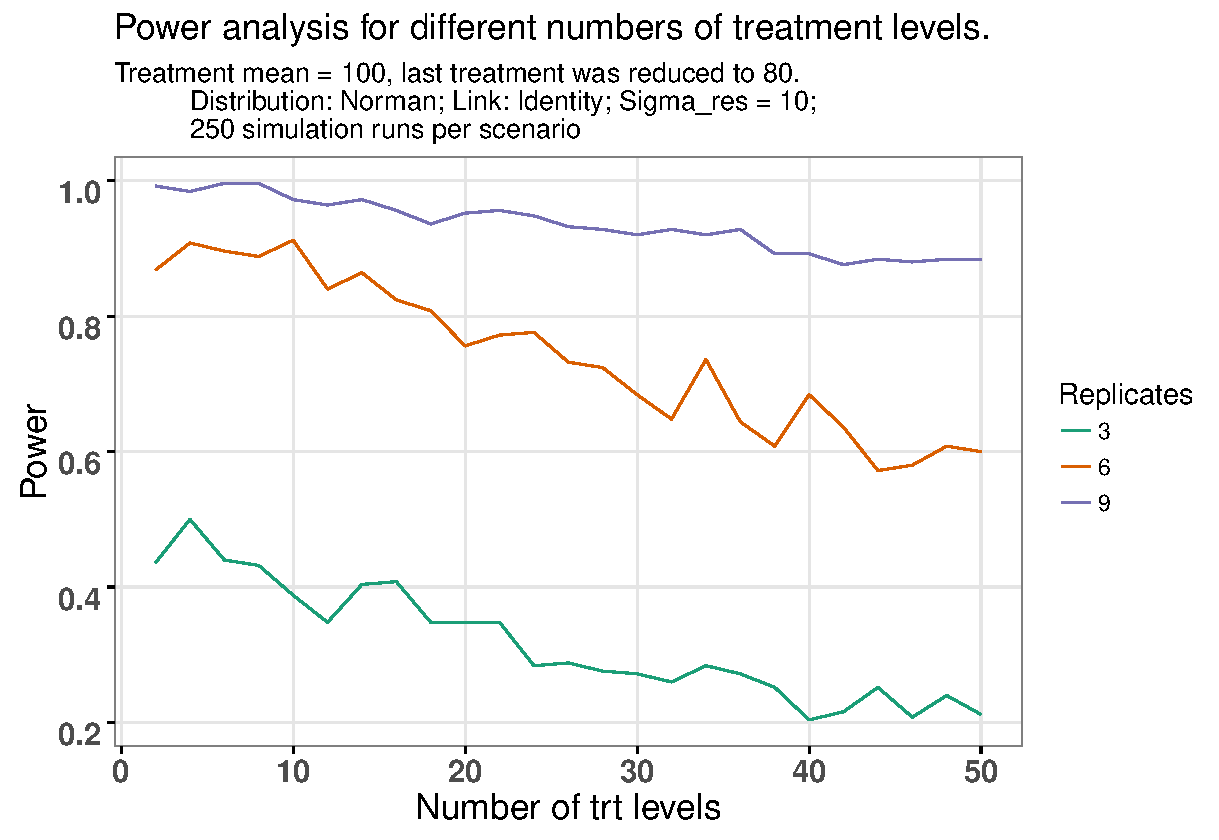
\includegraphics[width =0.9\textwidth]{figs/p_power_trt.pdf} 
	\\ \footnotesize Source code: \url{http://uni-ko-ld.de/gz}
\end{frame}


\begin{frame}
\frametitle{Comparison with Ives...}
	\begin{columns}[T]
	    \column{.49\textwidth}
	    	\underline{Szöcs (2015)}
	    	\begin{itemize}
	        	\item factorial design
	        	\item one predictor
	        	\item low replicated
	        	\item LM, GLM, bootstrap
	        	\item High T1 error of NB
	        	\item Quasi-Poisson worked well \vspace{1.2em}
	        	\item Bootstrap fixes the problems
	        \end{itemize}
	    \column{.49\textwidth}
	    	\underline{Ives (2015)}
	        \begin{itemize}
	        	\item continuous design
	        	\item two predictors
	        	\item well replicated
	        	\item LM, GLM
	        	\item High T1 error of NB
	        	\item Quasi-Poisson has problems with multiple predictors
	        	\item
	        \end{itemize}
	\end{columns}
\end{frame}


\begin{frame}
\frametitle{Simulations are worth their work, use them \emph{a priori}!}
\begingroup
\footnotesize % = 10pt in 12pt default
	Experimental design for dose-response experiments - a simulation \\
	\url{http://edild.github.io/lc50_bias_sim/}
		    	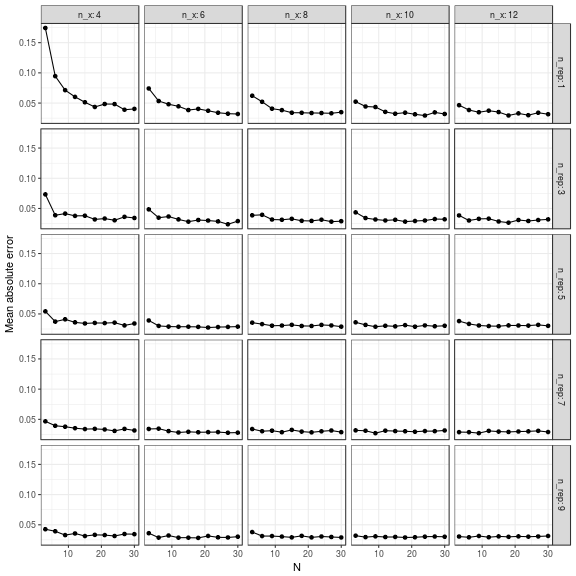
\includegraphics[width=0.5\textwidth, keepaspectratio]{figs/sim_drm.png} \\
	\begin{description}
		\item[GLM-Explorer:]{\url{http://uni-ko-ld.de/g3}}
	\end{description}
\endgroup
\end{frame}


{
\setbeamertemplate{frame footer}{Arle et al. (2016). Monitoring of Surface Waters in Germany under the Water Framework Directive - A Review of Approaches, Methods and Results. Water 8, 217–239
}
\begin{frame}
\frametitle{Aims of Environmental Monitoring of the WFD}
	\begin{itemize}
			\item assess \alert{status}
			\item observe \alert{trends}
			\item determine \alert{effects}
			\item basis for \alert{planning}
			\item control \alert{effectiveness} of measures
			\item prevent \alert{dangers}
	\end{itemize}
\end{frame}
}



\begin{frame}
	\frametitle{Idiosyncrasies of chemical concentrations}
	\begin{columns}[T]
	\column{.4\textwidth}
		\footnotesize
		\vspace{1em}
		\begin{itemize}
		\item continuous distribution in $\mathbb{R}^{+}_0$
		\item censoring \\ (x \textless LOQ )
		\item non-linearity \\ (season, trends)
		\item dependency \\(spatial, temporal)
		\item missing data
		\end{itemize}
	\column{.6\textwidth}
		\colorbox{white}{\includegraphics<1->[width =\textwidth]{figs/glyph.pdf}}
	\end{columns}
\end{frame}




\begin{frame}
\frametitle{ZAGA what...?}
	\begin{description}
		% \item[shiny app: ]{\url{http://139.14.11.23:3838/teaching/zaga/}}
		\item[shiny app: ]{\url{http://uni-ko-ld.de/g4}}
	\end{description}
	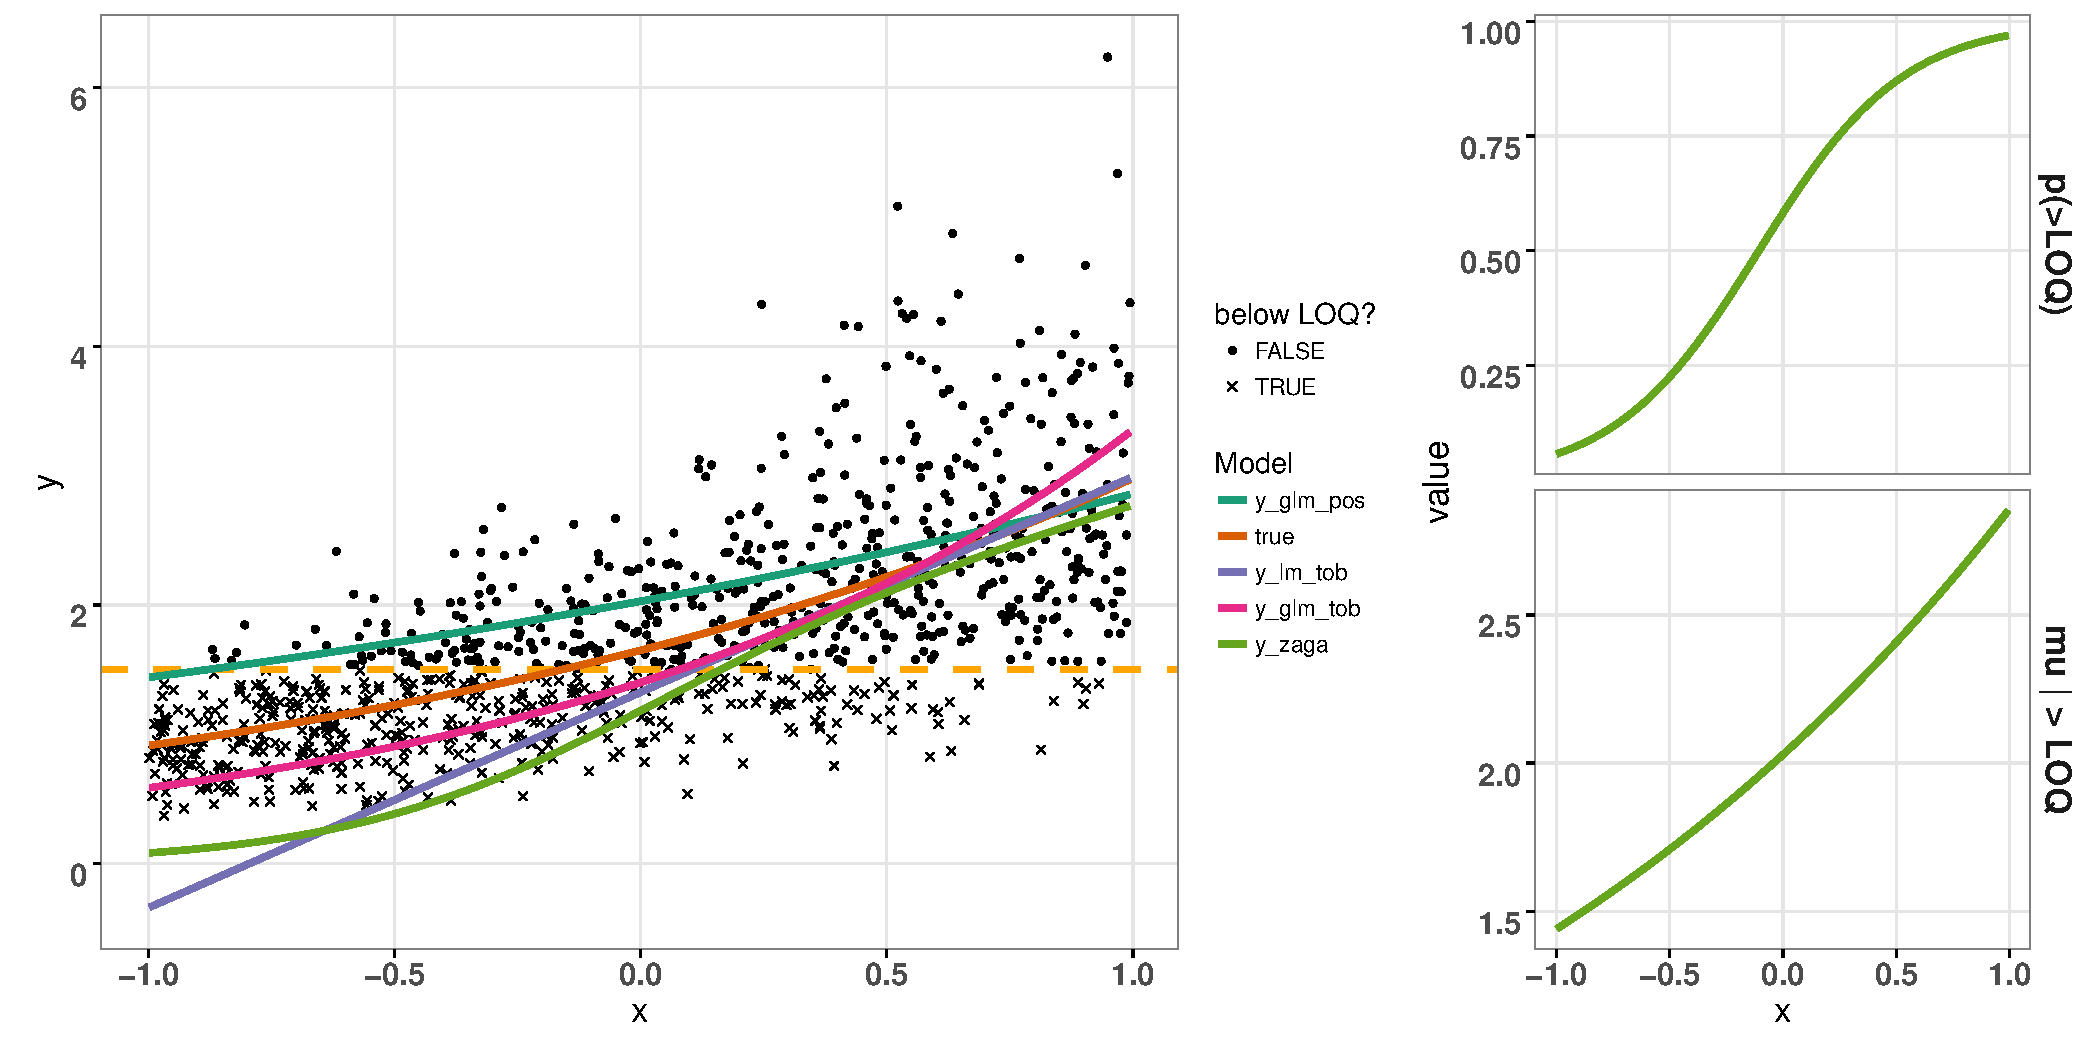
\includegraphics[width=1.1\textwidth]{figs/zaga_mods.pdf}
\end{frame}



\begin{frame}
	\frametitle{Model Performance}
	\begin{columns}[T]
	\column{.45\textwidth}
		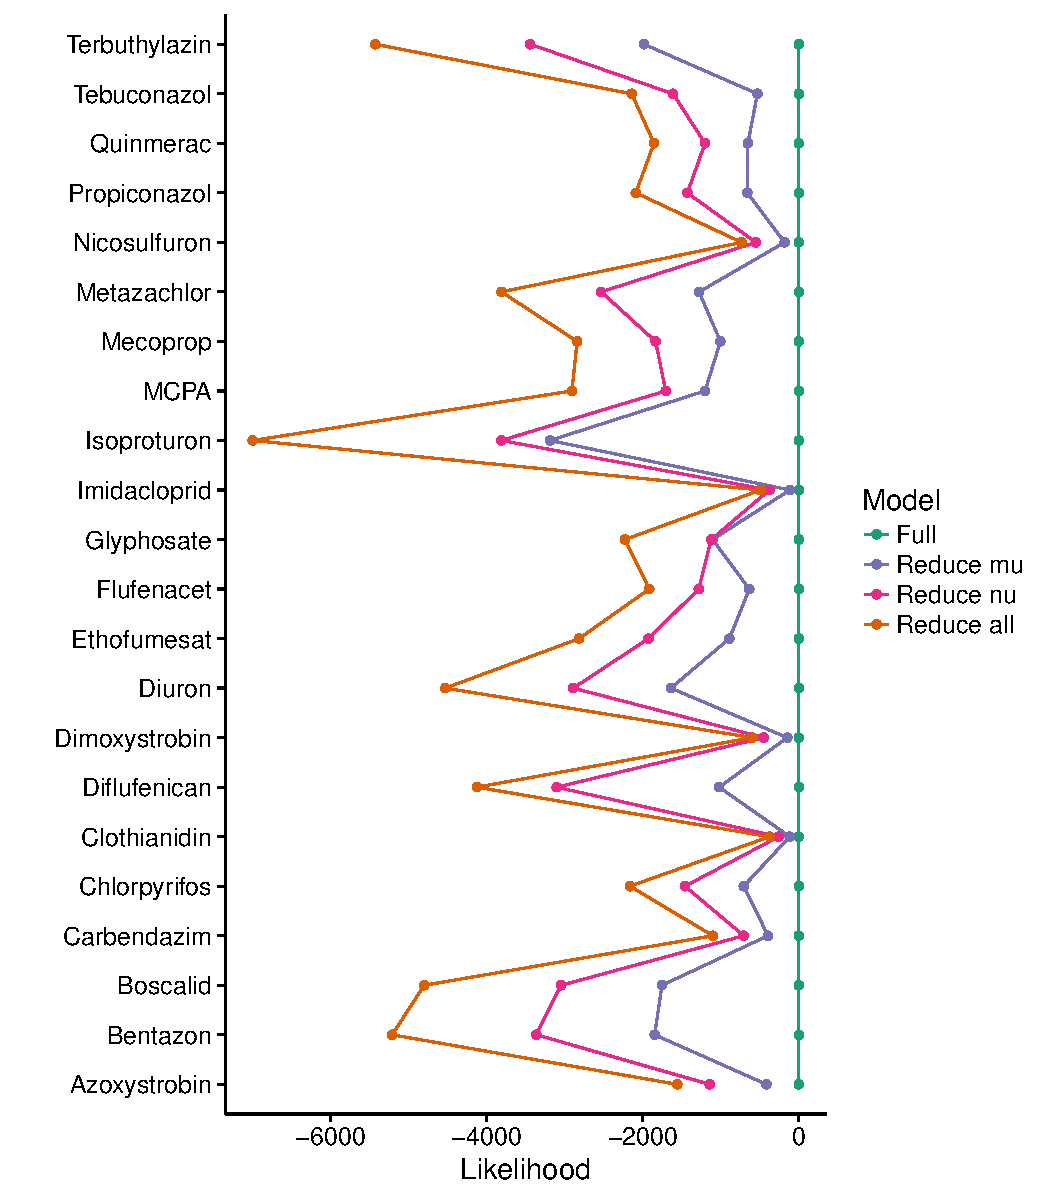
\includegraphics[width =1.1\textwidth]{figs/logliks.pdf}
	\column{.55\textwidth}
		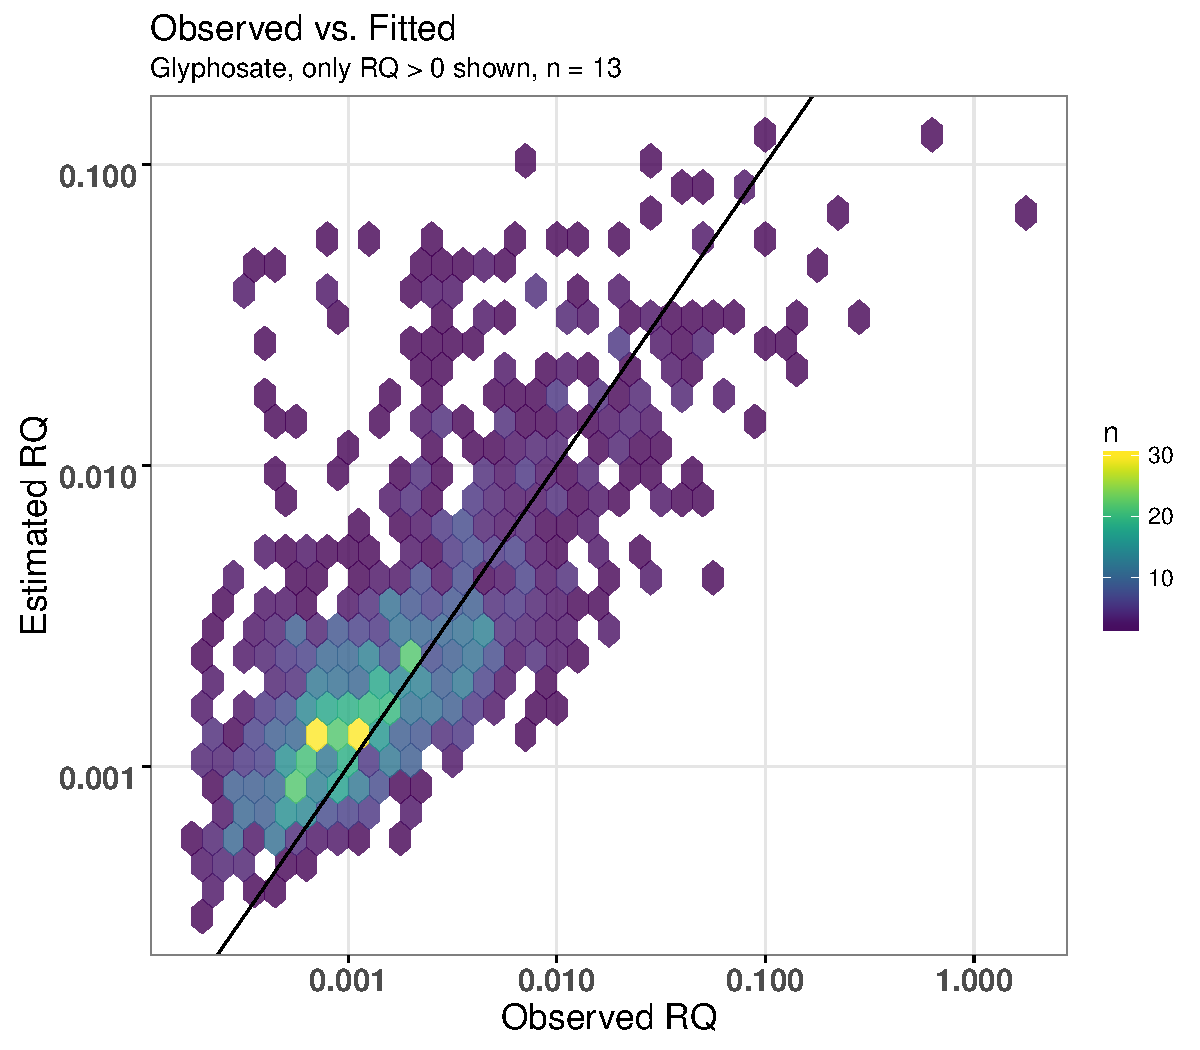
\includegraphics[width =1.1\textwidth]{figs/pftdvsobs.pdf}
	\end{columns}
\end{frame}



\begin{frame}
\frametitle{Stream size - width relationship}
	  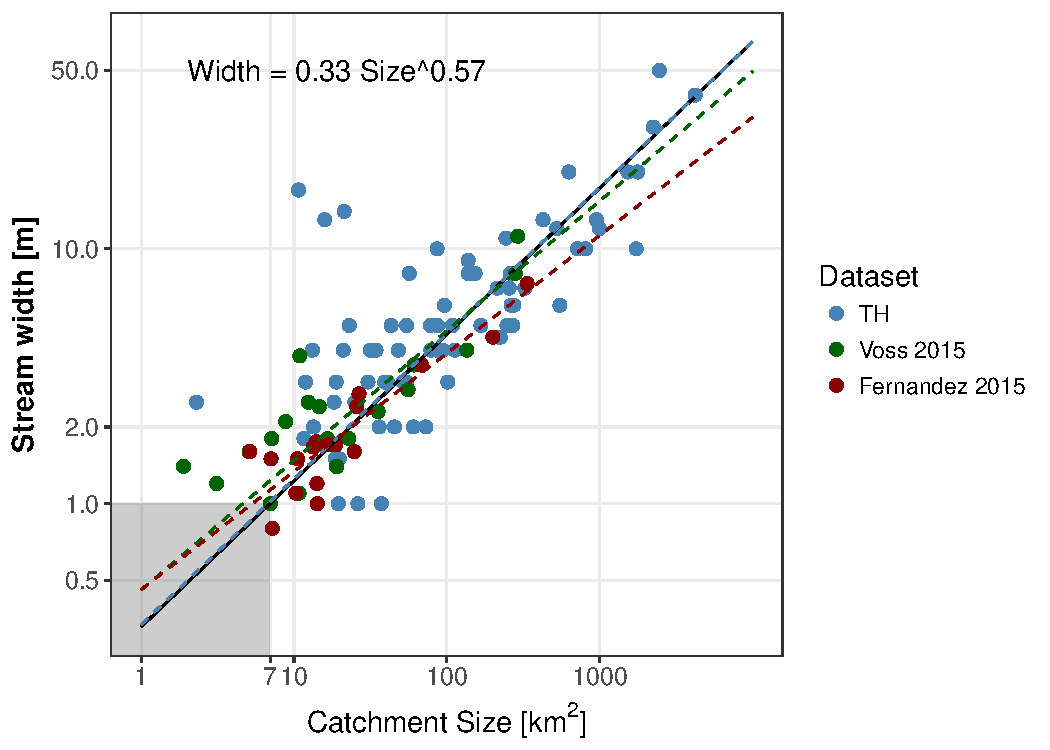
\includegraphics[width=\textwidth]{figs/width_size.pdf}
\end{frame}


{
\setbeamertemplate{frame footer}{Biggs et al. (2016). The importance of small waterbodies for biodiversity and ecosystem services: implications for policy makers. Hydrobiologia. DOI: 10.1007/s10750-016-3007-0. 
}
\begin{frame}
\frametitle{Small streams in the landscape}
	\hspace*{-10mm}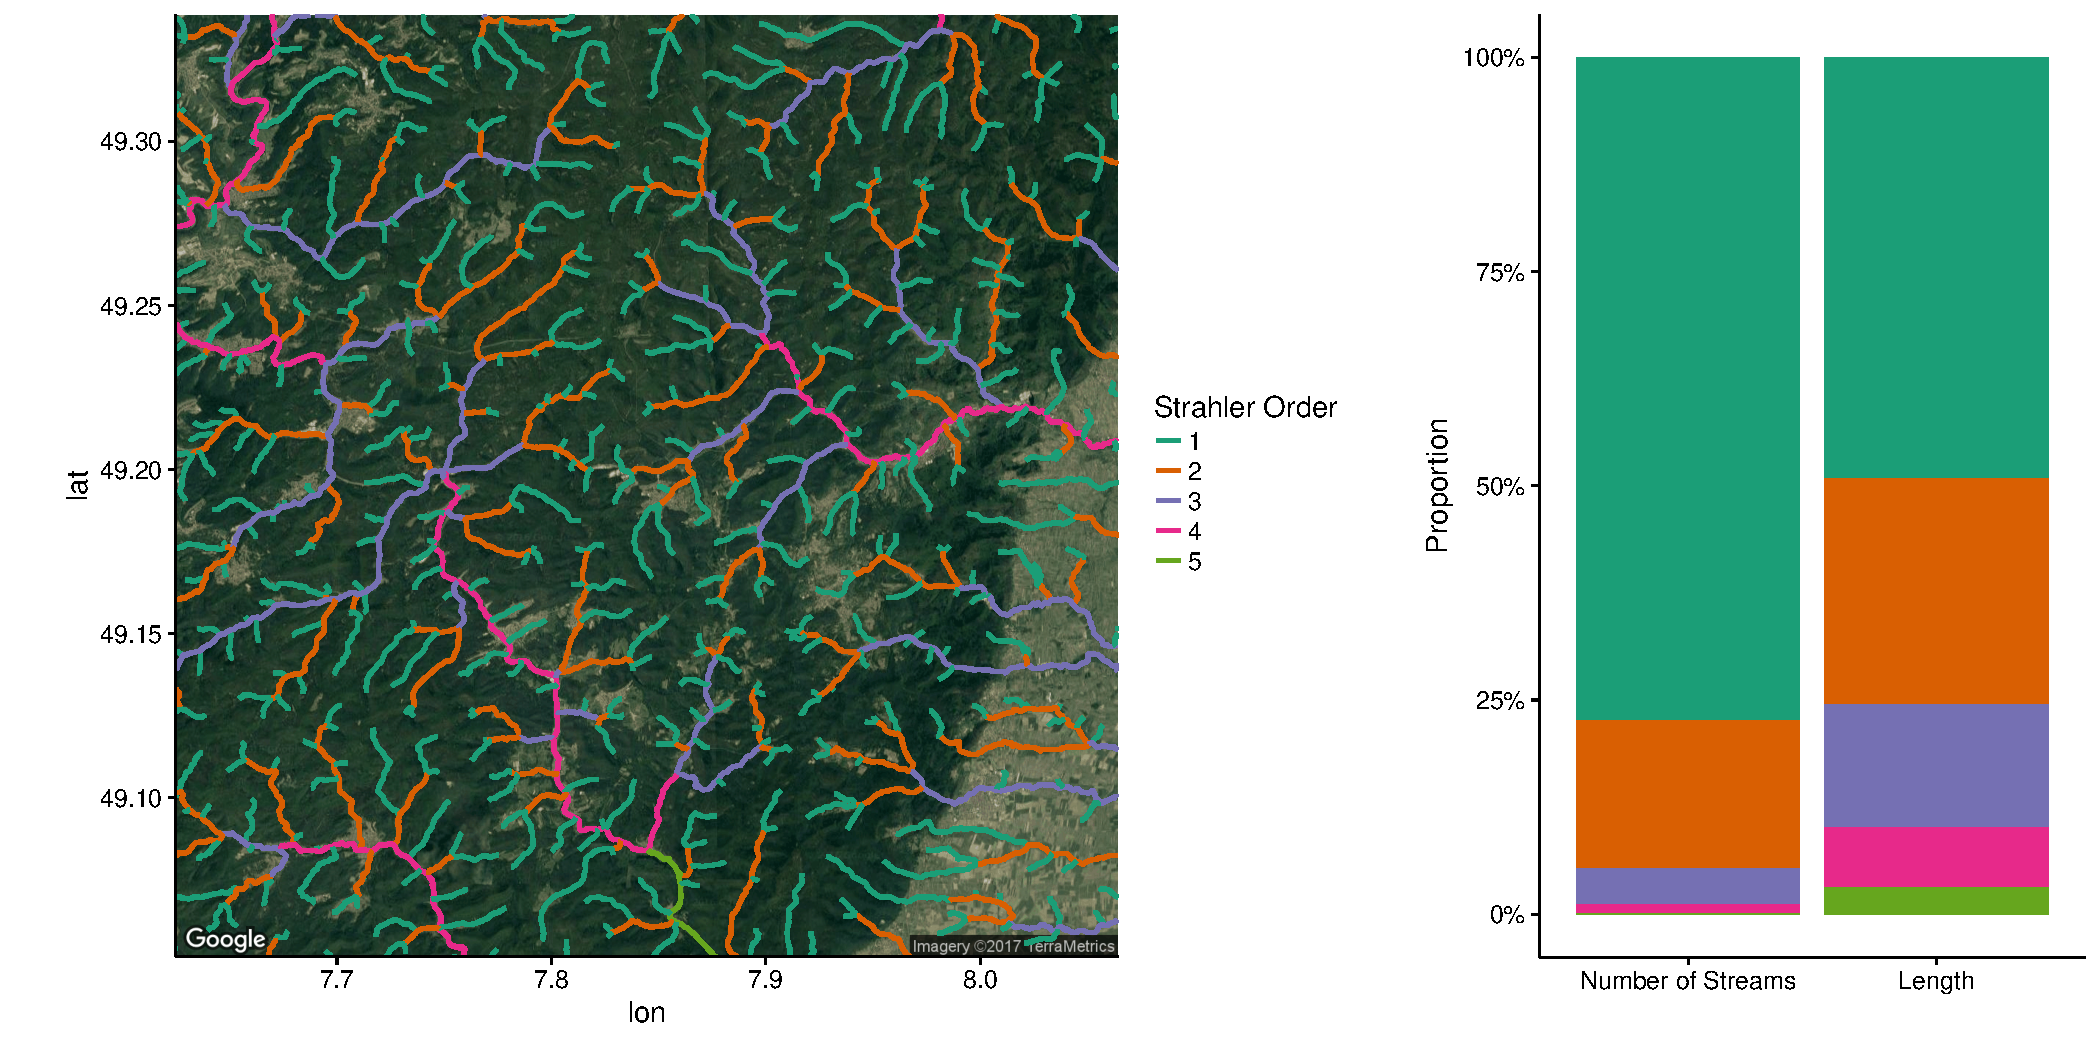
\includegraphics[width=1.1\textwidth]{figs/streams_distr.pdf}
	\vspace*{-10mm}
	\begingroup
	\footnotesize
	\begin{itemize}
		\item Biodiversity
		\item Refuge for re-colonisation
	\end{itemize}
	\endgroup
\end{frame}
}


\begin{frame}
\frametitle{Precipitation in Germany and the samples}
	\begin{columns}
	    \column{.49\textwidth}
	    	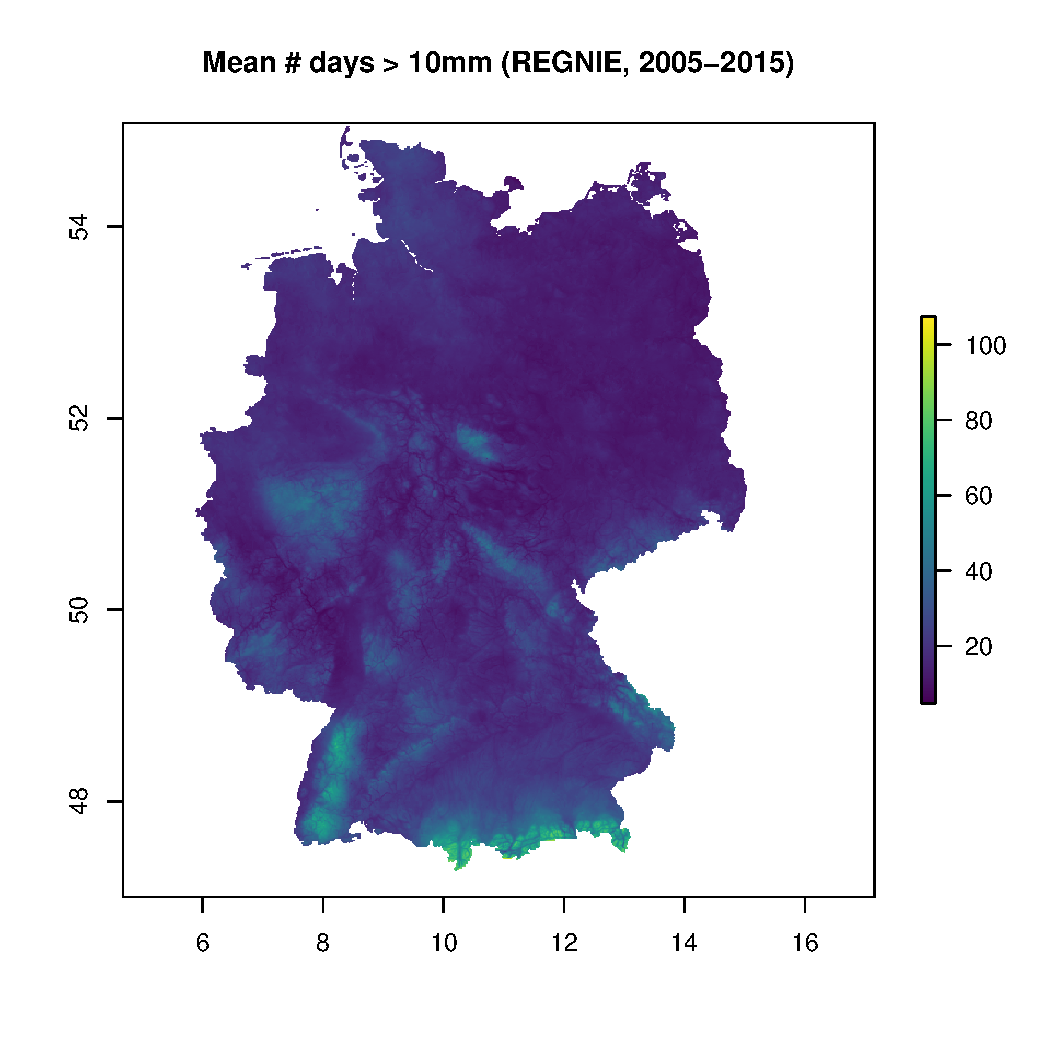
\includegraphics[width=1.1\textwidth, keepaspectratio]{figs/precip_map.pdf}
	    \column{.49\textwidth}
	    	    	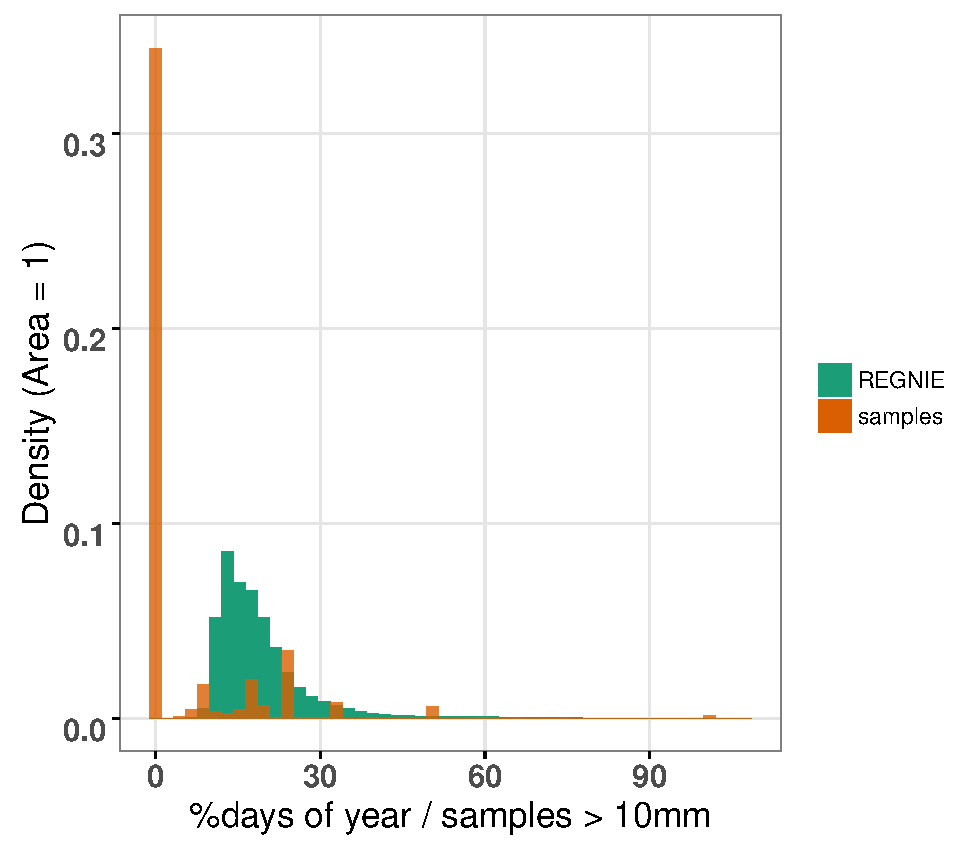
\includegraphics[width=1.1\textwidth, keepaspectratio]{figs/precip_comp.pdf}
	\end{columns}
\end{frame}



\begin{frame}[shrink]
\frametitle{Comparison with other studies}
	\begin{columns}[T]
	    \column{.33\textwidth}
	    \underline{Szöcs (2016)}
	    \begin{itemize}
        	\item Germany \\[1.5em]
        	\item Monitoring
        	\item Grab sampling \vspace{1.2em}
        	\item Pesticides
        	\item Neonics + Chlorpyrifos
        	\item ZAGA (\textless LOQ)
        	\item CS: no
        \end{itemize}
	    \column{.33\textwidth}
	    \underline{Stehle (2015)}
	    \begin{itemize}
        	\item Europe / Global
        	\item Publications
        	\item Grab \& Event driven sampling
        	\item Insecticides
        	\item Organophos.+ Pyrethroids
        	\item LM for \textgreater LOQ
        	\item CS: weak (-0.26 per log CS)
        \end{itemize}
	    \column{.33\textwidth}
	    \underline{Knauer (2016)}
	    \begin{itemize}
        	\item Switzerland \\[1.5em]
        	\item Monitoring
        	\item Grab sampling \vspace{1.2em}
        	\item Pesticides
        	\item Chlorpyrifos + Herb + Fung 
        	\item no model
        	\item CS: (yes)
        \end{itemize}
	\end{columns}
\end{frame}


\begin{frame}
\frametitle{RACs by Type}
	\begin{adjustbox}{max totalsize={\textwidth}{0.95\textheight}}
				% Created by tikzDevice version 0.10.1 on 2016-12-09 10:11:42
% !TEX encoding = UTF-8 Unicode
\begin{tikzpicture}[x=1pt,y=1pt]
\definecolor{fillColor}{RGB}{255,255,255}
\path[use as bounding box,fill=fillColor,fill opacity=0.00] (0,0) rectangle (505.89,361.35);
\begin{scope}
\path[clip] (  0.00,  0.00) rectangle (505.89,361.35);
\definecolor{drawColor}{RGB}{255,255,255}
\definecolor{fillColor}{RGB}{255,255,255}

\path[draw=drawColor,line width= 0.6pt,line join=round,line cap=round,fill=fillColor] (  0.00,  0.00) rectangle (505.89,361.35);
\end{scope}
\begin{scope}
\path[clip] ( 87.99, 41.00) rectangle (498.89,332.44);
\definecolor{fillColor}{RGB}{255,255,255}

\path[fill=fillColor] ( 87.99, 41.00) rectangle (498.89,332.44);
\definecolor{drawColor}{gray}{0.90}

\path[draw=drawColor,line width= 0.6pt,line join=round] ( 87.99, 68.70) --
	(498.89, 68.70);

\path[draw=drawColor,line width= 0.6pt,line join=round] ( 87.99,110.22) --
	(498.89,110.22);

\path[draw=drawColor,line width= 0.6pt,line join=round] ( 87.99,151.73) --
	(498.89,151.73);

\path[draw=drawColor,line width= 0.6pt,line join=round] ( 87.99,193.25) --
	(498.89,193.25);

\path[draw=drawColor,line width= 0.6pt,line join=round] ( 87.99,234.77) --
	(498.89,234.77);

\path[draw=drawColor,line width= 0.6pt,line join=round] ( 87.99,276.28) --
	(498.89,276.28);

\path[draw=drawColor,line width= 0.6pt,line join=round] ( 87.99,317.80) --
	(498.89,317.80);

\path[draw=drawColor,line width= 0.6pt,line join=round] (146.69, 41.00) --
	(146.69,332.44);

\path[draw=drawColor,line width= 0.6pt,line join=round] (244.52, 41.00) --
	(244.52,332.44);

\path[draw=drawColor,line width= 0.6pt,line join=round] (342.36, 41.00) --
	(342.36,332.44);

\path[draw=drawColor,line width= 0.6pt,line join=round] (440.19, 41.00) --
	(440.19,332.44);
\definecolor{drawColor}{gray}{0.20}
\definecolor{fillColor}{gray}{0.20}

\path[draw=drawColor,line width= 0.4pt,line join=round,line cap=round,fill=fillColor] (146.69,287.76) circle (  1.96);

\path[draw=drawColor,line width= 0.6pt,line join=round] (146.69,222.59) -- (146.69,262.28);

\path[draw=drawColor,line width= 0.6pt,line join=round] (146.69,179.62) -- (146.69,130.96);
\definecolor{fillColor}{gray}{0.75}

\path[draw=drawColor,line width= 0.6pt,line join=round,line cap=round,fill=fillColor] (110.00,222.59) --
	(110.00,179.62) --
	(183.38,179.62) --
	(183.38,222.59) --
	(110.00,222.59) --
	cycle;

\path[draw=drawColor,line width= 1.1pt,line join=round] (110.00,194.11) -- (183.38,194.11);
\definecolor{fillColor}{gray}{0.20}

\path[draw=drawColor,line width= 0.4pt,line join=round,line cap=round,fill=fillColor] (244.52,319.19) circle (  1.96);

\path[draw=drawColor,line width= 0.6pt,line join=round] (244.52,238.05) -- (244.52,306.52);

\path[draw=drawColor,line width= 0.6pt,line join=round] (244.52,187.24) -- (244.52,126.74);
\definecolor{fillColor}{gray}{0.75}

\path[draw=drawColor,line width= 0.6pt,line join=round,line cap=round,fill=fillColor] (207.84,238.05) --
	(207.84,187.24) --
	(281.21,187.24) --
	(281.21,238.05) --
	(207.84,238.05) --
	cycle;

\path[draw=drawColor,line width= 1.1pt,line join=round] (207.84,205.75) -- (281.21,205.75);
\definecolor{fillColor}{gray}{0.20}

\path[draw=drawColor,line width= 0.4pt,line join=round,line cap=round,fill=fillColor] (342.36,296.68) circle (  1.96);

\path[draw=drawColor,line width= 0.6pt,line join=round] (342.36,179.24) -- (342.36,234.77);

\path[draw=drawColor,line width= 0.6pt,line join=round] (342.36,101.26) -- (342.36, 54.30);
\definecolor{fillColor}{gray}{0.75}

\path[draw=drawColor,line width= 0.6pt,line join=round,line cap=round,fill=fillColor] (305.67,179.24) --
	(305.67,101.26) --
	(379.04,101.26) --
	(379.04,179.24) --
	(305.67,179.24) --
	cycle;

\path[draw=drawColor,line width= 1.1pt,line join=round] (305.67,134.13) -- (379.04,134.13);

\path[draw=drawColor,line width= 0.6pt,line join=round] (440.19,246.37) -- (440.19,286.88);

\path[draw=drawColor,line width= 0.6pt,line join=round] (440.19,210.62) -- (440.19,194.97);

\path[draw=drawColor,line width= 0.6pt,line join=round,line cap=round,fill=fillColor] (403.50,246.37) --
	(403.50,210.62) --
	(476.88,210.62) --
	(476.88,246.37) --
	(403.50,246.37) --
	cycle;

\path[draw=drawColor,line width= 1.1pt,line join=round] (403.50,224.35) -- (476.88,224.35);
\definecolor{drawColor}{RGB}{0,0,0}
\definecolor{fillColor}{RGB}{0,0,0}

\path[draw=drawColor,line width= 0.4pt,line join=round,line cap=round,fill=fillColor] (454.28,194.99) circle (  1.96);

\path[draw=drawColor,line width= 0.4pt,line join=round,line cap=round,fill=fillColor] (450.89,232.93) circle (  1.96);

\path[draw=drawColor,line width= 0.4pt,line join=round,line cap=round,fill=fillColor] (336.02,167.55) circle (  1.96);

\path[draw=drawColor,line width= 0.4pt,line join=round,line cap=round,fill=fillColor] (234.91,194.27) circle (  1.96);

\path[draw=drawColor,line width= 0.4pt,line join=round,line cap=round,fill=fillColor] (141.99,182.49) circle (  1.96);

\path[draw=drawColor,line width= 0.4pt,line join=round,line cap=round,fill=fillColor] (132.00,247.20) circle (  1.96);

\path[draw=drawColor,line width= 0.4pt,line join=round,line cap=round,fill=fillColor] (257.31,306.53) circle (  1.96);

\path[draw=drawColor,line width= 0.4pt,line join=round,line cap=round,fill=fillColor] (338.11, 56.14) circle (  1.96);

\path[draw=drawColor,line width= 0.4pt,line join=round,line cap=round,fill=fillColor] (157.51,179.23) circle (  1.96);

\path[draw=drawColor,line width= 0.4pt,line join=round,line cap=round,fill=fillColor] (136.20,238.79) circle (  1.96);

\path[draw=drawColor,line width= 0.4pt,line join=round,line cap=round,fill=fillColor] (250.95,214.79) circle (  1.96);

\path[draw=drawColor,line width= 0.4pt,line join=round,line cap=round,fill=fillColor] (159.92,222.31) circle (  1.96);

\path[draw=drawColor,line width= 0.4pt,line join=round,line cap=round,fill=fillColor] (130.01,159.02) circle (  1.96);

\path[draw=drawColor,line width= 0.4pt,line join=round,line cap=round,fill=fillColor] (259.30,172.10) circle (  1.96);

\path[draw=drawColor,line width= 0.4pt,line join=round,line cap=round,fill=fillColor] (348.87,174.51) circle (  1.96);

\path[draw=drawColor,line width= 0.4pt,line join=round,line cap=round,fill=fillColor] (242.04,265.81) circle (  1.96);

\path[draw=drawColor,line width= 0.4pt,line join=round,line cap=round,fill=fillColor] (437.47,215.90) circle (  1.96);

\path[draw=drawColor,line width= 0.4pt,line join=round,line cap=round,fill=fillColor] (341.51, 54.25) circle (  1.96);

\path[draw=drawColor,line width= 0.4pt,line join=round,line cap=round,fill=fillColor] (261.29,208.26) circle (  1.96);

\path[draw=drawColor,line width= 0.4pt,line join=round,line cap=round,fill=fillColor] (227.49,224.47) circle (  1.96);

\path[draw=drawColor,line width= 0.4pt,line join=round,line cap=round,fill=fillColor] (262.09,319.14) circle (  1.96);

\path[draw=drawColor,line width= 0.4pt,line join=round,line cap=round,fill=fillColor] (328.17,103.83) circle (  1.96);

\path[draw=drawColor,line width= 0.4pt,line join=round,line cap=round,fill=fillColor] (358.78,193.19) circle (  1.96);

\path[draw=drawColor,line width= 0.4pt,line join=round,line cap=round,fill=fillColor] (136.76,219.99) circle (  1.96);

\path[draw=drawColor,line width= 0.4pt,line join=round,line cap=round,fill=fillColor] (353.97, 68.69) circle (  1.96);

\path[draw=drawColor,line width= 0.4pt,line join=round,line cap=round,fill=fillColor] (135.36,188.09) circle (  1.96);

\path[draw=drawColor,line width= 0.4pt,line join=round,line cap=round,fill=fillColor] (456.78,286.85) circle (  1.96);

\path[draw=drawColor,line width= 0.4pt,line join=round,line cap=round,fill=fillColor] (137.53,174.90) circle (  1.96);

\path[draw=drawColor,line width= 0.4pt,line join=round,line cap=round,fill=fillColor] (232.12,126.74) circle (  1.96);

\path[draw=drawColor,line width= 0.4pt,line join=round,line cap=round,fill=fillColor] (236.13,189.93) circle (  1.96);

\path[draw=drawColor,line width= 0.4pt,line join=round,line cap=round,fill=fillColor] (233.34,215.77) circle (  1.96);

\path[draw=drawColor,line width= 0.4pt,line join=round,line cap=round,fill=fillColor] (240.13,198.70) circle (  1.96);

\path[draw=drawColor,line width= 0.4pt,line join=round,line cap=round,fill=fillColor] (356.79,218.21) circle (  1.96);

\path[draw=drawColor,line width= 0.4pt,line join=round,line cap=round,fill=fillColor] (153.97,224.25) circle (  1.96);

\path[draw=drawColor,line width= 0.4pt,line join=round,line cap=round,fill=fillColor] (152.98,130.90) circle (  1.96);

\path[draw=drawColor,line width= 0.4pt,line join=round,line cap=round,fill=fillColor] (160.95,188.78) circle (  1.96);

\path[draw=drawColor,line width= 0.4pt,line join=round,line cap=round,fill=fillColor] (243.96,188.98) circle (  1.96);

\path[draw=drawColor,line width= 0.4pt,line join=round,line cap=round,fill=fillColor] (166.00,223.49) circle (  1.96);

\path[draw=drawColor,line width= 0.4pt,line join=round,line cap=round,fill=fillColor] (156.49,181.99) circle (  1.96);

\path[draw=drawColor,line width= 0.4pt,line join=round,line cap=round,fill=fillColor] (250.39,250.48) circle (  1.96);

\path[draw=drawColor,line width= 0.4pt,line join=round,line cap=round,fill=fillColor] (156.58,234.97) circle (  1.96);

\path[draw=drawColor,line width= 0.4pt,line join=round,line cap=round,fill=fillColor] (165.48,163.83) circle (  1.96);

\path[draw=drawColor,line width= 0.4pt,line join=round,line cap=round,fill=fillColor] (350.30, 64.00) circle (  1.96);

\path[draw=drawColor,line width= 0.4pt,line join=round,line cap=round,fill=fillColor] (326.43,296.74) circle (  1.96);

\path[draw=drawColor,line width= 0.4pt,line join=round,line cap=round,fill=fillColor] (244.06,283.11) circle (  1.96);

\path[draw=drawColor,line width= 0.4pt,line join=round,line cap=round,fill=fillColor] (237.19,230.02) circle (  1.96);

\path[draw=drawColor,line width= 0.4pt,line join=round,line cap=round,fill=fillColor] (158.16,168.90) circle (  1.96);

\path[draw=drawColor,line width= 0.4pt,line join=round,line cap=round,fill=fillColor] (159.70,180.78) circle (  1.96);

\path[draw=drawColor,line width= 0.4pt,line join=round,line cap=round,fill=fillColor] (244.34,209.02) circle (  1.96);

\path[draw=drawColor,line width= 0.4pt,line join=round,line cap=round,fill=fillColor] (163.89,222.70) circle (  1.96);

\path[draw=drawColor,line width= 0.4pt,line join=round,line cap=round,fill=fillColor] (143.78,189.23) circle (  1.96);

\path[draw=drawColor,line width= 0.4pt,line join=round,line cap=round,fill=fillColor] (231.60,172.43) circle (  1.96);

\path[draw=drawColor,line width= 0.4pt,line join=round,line cap=round,fill=fillColor] (244.91,243.25) circle (  1.96);

\path[draw=drawColor,line width= 0.4pt,line join=round,line cap=round,fill=fillColor] (247.46,193.06) circle (  1.96);

\path[draw=drawColor,line width= 0.4pt,line join=round,line cap=round,fill=fillColor] (136.16,194.97) circle (  1.96);

\path[draw=drawColor,line width= 0.4pt,line join=round,line cap=round,fill=fillColor] (257.73,150.76) circle (  1.96);

\path[draw=drawColor,line width= 0.4pt,line join=round,line cap=round,fill=fillColor] (248.79,276.35) circle (  1.96);

\path[draw=drawColor,line width= 0.4pt,line join=round,line cap=round,fill=fillColor] (329.17,108.24) circle (  1.96);

\path[draw=drawColor,line width= 0.4pt,line join=round,line cap=round,fill=fillColor] (260.15,147.48) circle (  1.96);

\path[draw=drawColor,line width= 0.4pt,line join=round,line cap=round,fill=fillColor] (256.17,211.11) circle (  1.96);

\path[draw=drawColor,line width= 0.4pt,line join=round,line cap=round,fill=fillColor] (132.69,287.77) circle (  1.96);

\path[draw=drawColor,line width= 0.4pt,line join=round,line cap=round,fill=fillColor] (227.93,197.91) circle (  1.96);

\path[draw=drawColor,line width= 0.4pt,line join=round,line cap=round,fill=fillColor] (139.97,193.22) circle (  1.96);

\path[draw=drawColor,line width= 0.4pt,line join=round,line cap=round,fill=fillColor] (226.65,185.48) circle (  1.96);

\path[draw=drawColor,line width= 0.4pt,line join=round,line cap=round,fill=fillColor] (150.12,165.90) circle (  1.96);

\path[draw=drawColor,line width= 0.4pt,line join=round,line cap=round,fill=fillColor] (141.13,229.84) circle (  1.96);

\path[draw=drawColor,line width= 0.4pt,line join=round,line cap=round,fill=fillColor] (255.06,232.83) circle (  1.96);

\path[draw=drawColor,line width= 0.4pt,line join=round,line cap=round,fill=fillColor] (234.05,284.70) circle (  1.96);

\path[draw=drawColor,line width= 0.4pt,line join=round,line cap=round,fill=fillColor] (161.88,262.30) circle (  1.96);

\path[draw=drawColor,line width= 0.4pt,line join=round,line cap=round,fill=fillColor] (250.28,258.85) circle (  1.96);

\path[draw=drawColor,line width= 0.4pt,line join=round,line cap=round,fill=fillColor] (250.38,190.89) circle (  1.96);

\path[draw=drawColor,line width= 0.4pt,line join=round,line cap=round,fill=fillColor] (355.34,110.25) circle (  1.96);

\path[draw=drawColor,line width= 0.4pt,line join=round,line cap=round,fill=fillColor] (248.64,205.74) circle (  1.96);

\path[draw=drawColor,line width= 0.4pt,line join=round,line cap=round,fill=fillColor] (251.49,183.54) circle (  1.96);

\path[draw=drawColor,line width= 0.4pt,line join=round,line cap=round,fill=fillColor] (160.07,209.00) circle (  1.96);

\path[draw=drawColor,line width= 0.4pt,line join=round,line cap=round,fill=fillColor] (262.31,227.49) circle (  1.96);

\path[draw=drawColor,line width= 0.4pt,line join=round,line cap=round,fill=fillColor] (247.26,148.84) circle (  1.96);

\path[draw=drawColor,line width= 0.4pt,line join=round,line cap=round,fill=fillColor] (345.68,194.93) circle (  1.96);

\path[draw=drawColor,line width= 0.4pt,line join=round,line cap=round,fill=fillColor] (150.64,214.19) circle (  1.96);

\path[draw=drawColor,line width= 0.4pt,line join=round,line cap=round,fill=fillColor] (234.92,184.88) circle (  1.96);

\path[draw=drawColor,line width= 0.4pt,line join=round,line cap=round,fill=fillColor] (252.36,203.56) circle (  1.96);

\path[draw=drawColor,line width= 0.4pt,line join=round,line cap=round,fill=fillColor] (225.95,133.30) circle (  1.96);

\path[draw=drawColor,line width= 0.4pt,line join=round,line cap=round,fill=fillColor] (165.62,184.10) circle (  1.96);

\path[draw=drawColor,line width= 0.4pt,line join=round,line cap=round,fill=fillColor] (337.61,149.79) circle (  1.96);

\path[draw=drawColor,line width= 0.4pt,line join=round,line cap=round,fill=fillColor] (142.58,222.30) circle (  1.96);

\path[draw=drawColor,line width= 0.4pt,line join=round,line cap=round,fill=fillColor] (129.70,205.68) circle (  1.96);

\path[draw=drawColor,line width= 0.4pt,line join=round,line cap=round,fill=fillColor] (232.52,256.89) circle (  1.96);

\path[draw=drawColor,line width= 0.4pt,line join=round,line cap=round,fill=fillColor] (254.45,217.31) circle (  1.96);

\path[draw=drawColor,line width= 0.4pt,line join=round,line cap=round,fill=fillColor] (137.43,202.93) circle (  1.96);

\path[draw=drawColor,line width= 0.4pt,line join=round,line cap=round,fill=fillColor] (334.19,116.24) circle (  1.96);

\path[draw=drawColor,line width= 0.4pt,line join=round,line cap=round,fill=fillColor] (138.80,230.72) circle (  1.96);

\path[draw=drawColor,line width= 0.4pt,line join=round,line cap=round,fill=fillColor] (227.43,296.98) circle (  1.96);

\path[draw=drawColor,line width= 0.4pt,line join=round,line cap=round,fill=fillColor] (238.06,179.25) circle (  1.96);

\path[draw=drawColor,line width= 0.4pt,line join=round,line cap=round,fill=fillColor] (332.51,143.15) circle (  1.96);

\path[draw=drawColor,line width= 0.4pt,line join=round,line cap=round,fill=fillColor] (348.48,234.77) circle (  1.96);

\path[draw=drawColor,line width= 0.4pt,line join=round,line cap=round,fill=fillColor] (151.43,156.49) circle (  1.96);

\path[draw=drawColor,line width= 0.4pt,line join=round,line cap=round,fill=fillColor] (336.17,131.70) circle (  1.96);

\path[draw=drawColor,line width= 0.4pt,line join=round,line cap=round,fill=fillColor] (146.11,183.38) circle (  1.96);

\path[draw=drawColor,line width= 0.4pt,line join=round,line cap=round,fill=fillColor] (242.52,196.49) circle (  1.96);

\path[draw=drawColor,line width= 0.4pt,line join=round,line cap=round,fill=fillColor] (353.69, 93.67) circle (  1.96);

\path[draw=drawColor,line width= 0.4pt,line join=round,line cap=round,fill=fillColor] (325.85,136.54) circle (  1.96);

\path[draw=drawColor,line width= 0.4pt,line join=round,line cap=round,fill=fillColor] (148.02,153.42) circle (  1.96);

\path[draw=drawColor,line width= 0.4pt,line join=round,line cap=round,fill=fillColor] (253.27,191.34) circle (  1.96);

\path[draw=drawColor,line width= 0.4pt,line join=round,line cap=round,fill=fillColor] (153.31,215.27) circle (  1.96);

\path[draw=drawColor,line width= 0.4pt,line join=round,line cap=round,fill=fillColor] (157.36,149.01) circle (  1.96);
\definecolor{drawColor}{gray}{0.50}

\path[draw=drawColor,line width= 0.6pt,line join=round,line cap=round] ( 87.99, 41.00) rectangle (498.89,332.44);
\end{scope}
\begin{scope}
\path[clip] (  0.00,  0.00) rectangle (505.89,361.35);
\definecolor{drawColor}{gray}{0.30}

\node[text=drawColor,anchor=base east,inner sep=0pt, outer sep=0pt, scale=  1.12] at ( 81.69, 60.97) {\bfseries 0.001};

\node[text=drawColor,anchor=base east,inner sep=0pt, outer sep=0pt, scale=  1.12] at ( 81.69,102.49) {\bfseries 0.010};

\node[text=drawColor,anchor=base east,inner sep=0pt, outer sep=0pt, scale=  1.12] at ( 81.69,144.00) {\bfseries 0.100};

\node[text=drawColor,anchor=base east,inner sep=0pt, outer sep=0pt, scale=  1.12] at ( 81.69,185.52) {\bfseries 1.000};

\node[text=drawColor,anchor=base east,inner sep=0pt, outer sep=0pt, scale=  1.12] at ( 81.69,227.04) {\bfseries 10.000};

\node[text=drawColor,anchor=base east,inner sep=0pt, outer sep=0pt, scale=  1.12] at ( 81.69,268.55) {\bfseries 100.000};

\node[text=drawColor,anchor=base east,inner sep=0pt, outer sep=0pt, scale=  1.12] at ( 81.69,310.07) {\bfseries 1,000.000};
\end{scope}
\begin{scope}
\path[clip] (  0.00,  0.00) rectangle (505.89,361.35);
\definecolor{drawColor}{RGB}{0,0,0}

\path[draw=drawColor,line width= 0.6pt,line join=round] ( 84.49, 68.70) --
	( 87.99, 68.70);

\path[draw=drawColor,line width= 0.6pt,line join=round] ( 84.49,110.22) --
	( 87.99,110.22);

\path[draw=drawColor,line width= 0.6pt,line join=round] ( 84.49,151.73) --
	( 87.99,151.73);

\path[draw=drawColor,line width= 0.6pt,line join=round] ( 84.49,193.25) --
	( 87.99,193.25);

\path[draw=drawColor,line width= 0.6pt,line join=round] ( 84.49,234.77) --
	( 87.99,234.77);

\path[draw=drawColor,line width= 0.6pt,line join=round] ( 84.49,276.28) --
	( 87.99,276.28);

\path[draw=drawColor,line width= 0.6pt,line join=round] ( 84.49,317.80) --
	( 87.99,317.80);
\end{scope}
\begin{scope}
\path[clip] (  0.00,  0.00) rectangle (505.89,361.35);
\definecolor{drawColor}{RGB}{0,0,0}

\path[draw=drawColor,line width= 0.6pt,line join=round] (146.69, 37.50) --
	(146.69, 41.00);

\path[draw=drawColor,line width= 0.6pt,line join=round] (244.52, 37.50) --
	(244.52, 41.00);

\path[draw=drawColor,line width= 0.6pt,line join=round] (342.36, 37.50) --
	(342.36, 41.00);

\path[draw=drawColor,line width= 0.6pt,line join=round] (440.19, 37.50) --
	(440.19, 41.00);
\end{scope}
\begin{scope}
\path[clip] (  0.00,  0.00) rectangle (505.89,361.35);
\definecolor{drawColor}{gray}{0.30}

\node[text=drawColor,anchor=base,inner sep=0pt, outer sep=0pt, scale=  1.12] at (146.69, 26.97) {\bfseries fungicides};

\node[text=drawColor,anchor=base,inner sep=0pt, outer sep=0pt, scale=  1.12] at (244.52, 26.97) {\bfseries herbicides};

\node[text=drawColor,anchor=base,inner sep=0pt, outer sep=0pt, scale=  1.12] at (342.36, 26.97) {\bfseries insecticides};

\node[text=drawColor,anchor=base,inner sep=0pt, outer sep=0pt, scale=  1.12] at (440.19, 26.97) {\bfseries other};
\end{scope}
\begin{scope}
\path[clip] (  0.00,  0.00) rectangle (505.89,361.35);
\definecolor{drawColor}{RGB}{0,0,0}

\node[text=drawColor,rotate= 90.00,anchor=base,inner sep=0pt, outer sep=0pt, scale=  1.68] at ( 22.62,186.72) {RAC [ug/L]};
\end{scope}
\begin{scope}
\path[clip] (  0.00,  0.00) rectangle (505.89,361.35);
\definecolor{drawColor}{RGB}{0,0,0}

\node[text=drawColor,anchor=base,inner sep=0pt, outer sep=0pt, scale=  1.68] at (293.44,341.81) {105 RACs provided by UBA splitted by group};
\end{scope}
\end{tikzpicture}

	\end{adjustbox}
\end{frame}


\begin{frame}
\frametitle{RACs by Compound}
\begingroup
\footnotesize % = 10pt in 12pt default
	\begin{adjustbox}{max totalsize={\textwidth}{0.95\textheight}}
				% Created by tikzDevice version 0.10.1 on 2016-12-09 10:15:06
% !TEX encoding = UTF-8 Unicode
\begin{tikzpicture}[x=1pt,y=1pt]
\definecolor{fillColor}{RGB}{255,255,255}
\path[use as bounding box,fill=fillColor,fill opacity=0.00] (0,0) rectangle (433.62,433.62);
\begin{scope}
\path[clip] (  0.00,  0.00) rectangle (433.62,433.62);
\definecolor{drawColor}{RGB}{255,255,255}
\definecolor{fillColor}{RGB}{255,255,255}

\path[draw=drawColor,line width= 0.6pt,line join=round,line cap=round,fill=fillColor] (  0.00,  0.00) rectangle (433.62,433.62);
\end{scope}
\begin{scope}
\path[clip] (166.28, 80.72) rectangle (426.62,405.68);
\definecolor{fillColor}{RGB}{255,255,255}

\path[fill=fillColor] (166.28, 80.72) rectangle (426.62,405.68);
\definecolor{drawColor}{gray}{0.90}

\path[draw=drawColor,line width= 0.6pt,line join=round] (166.28, 87.17) --
	(426.62, 87.17);

\path[draw=drawColor,line width= 0.6pt,line join=round] (166.28, 97.93) --
	(426.62, 97.93);

\path[draw=drawColor,line width= 0.6pt,line join=round] (166.28,108.69) --
	(426.62,108.69);

\path[draw=drawColor,line width= 0.6pt,line join=round] (166.28,119.45) --
	(426.62,119.45);

\path[draw=drawColor,line width= 0.6pt,line join=round] (166.28,130.21) --
	(426.62,130.21);

\path[draw=drawColor,line width= 0.6pt,line join=round] (166.28,140.97) --
	(426.62,140.97);

\path[draw=drawColor,line width= 0.6pt,line join=round] (166.28,151.73) --
	(426.62,151.73);

\path[draw=drawColor,line width= 0.6pt,line join=round] (166.28,162.49) --
	(426.62,162.49);

\path[draw=drawColor,line width= 0.6pt,line join=round] (166.28,173.25) --
	(426.62,173.25);

\path[draw=drawColor,line width= 0.6pt,line join=round] (166.28,184.01) --
	(426.62,184.01);

\path[draw=drawColor,line width= 0.6pt,line join=round] (166.28,194.77) --
	(426.62,194.77);

\path[draw=drawColor,line width= 0.6pt,line join=round] (166.28,205.54) --
	(426.62,205.54);

\path[draw=drawColor,line width= 0.6pt,line join=round] (166.28,216.30) --
	(426.62,216.30);

\path[draw=drawColor,line width= 0.6pt,line join=round] (166.28,227.06) --
	(426.62,227.06);

\path[draw=drawColor,line width= 0.6pt,line join=round] (166.28,237.82) --
	(426.62,237.82);

\path[draw=drawColor,line width= 0.6pt,line join=round] (166.28,248.58) --
	(426.62,248.58);

\path[draw=drawColor,line width= 0.6pt,line join=round] (166.28,259.34) --
	(426.62,259.34);

\path[draw=drawColor,line width= 0.6pt,line join=round] (166.28,270.10) --
	(426.62,270.10);

\path[draw=drawColor,line width= 0.6pt,line join=round] (166.28,280.86) --
	(426.62,280.86);

\path[draw=drawColor,line width= 0.6pt,line join=round] (166.28,291.62) --
	(426.62,291.62);

\path[draw=drawColor,line width= 0.6pt,line join=round] (166.28,302.38) --
	(426.62,302.38);

\path[draw=drawColor,line width= 0.6pt,line join=round] (166.28,313.14) --
	(426.62,313.14);

\path[draw=drawColor,line width= 0.6pt,line join=round] (166.28,323.90) --
	(426.62,323.90);

\path[draw=drawColor,line width= 0.6pt,line join=round] (166.28,334.66) --
	(426.62,334.66);

\path[draw=drawColor,line width= 0.6pt,line join=round] (166.28,345.42) --
	(426.62,345.42);

\path[draw=drawColor,line width= 0.6pt,line join=round] (166.28,356.18) --
	(426.62,356.18);

\path[draw=drawColor,line width= 0.6pt,line join=round] (166.28,366.94) --
	(426.62,366.94);

\path[draw=drawColor,line width= 0.6pt,line join=round] (166.28,377.70) --
	(426.62,377.70);

\path[draw=drawColor,line width= 0.6pt,line join=round] (166.28,388.46) --
	(426.62,388.46);

\path[draw=drawColor,line width= 0.6pt,line join=round] (166.28,399.22) --
	(426.62,399.22);

\path[draw=drawColor,line width= 0.6pt,line join=round] (206.45, 80.72) --
	(206.45,405.68);

\path[draw=drawColor,line width= 0.6pt,line join=round] (288.14, 80.72) --
	(288.14,405.68);

\path[draw=drawColor,line width= 0.6pt,line join=round] (369.84, 80.72) --
	(369.84,405.68);
\definecolor{drawColor}{RGB}{255,0,0}
\definecolor{fillColor}{RGB}{255,0,0}

\path[draw=drawColor,line width= 0.4pt,line join=round,line cap=round,fill=fillColor] (178.12,399.22) circle (  2.50);

\path[draw=drawColor,line width= 0.4pt,line join=round,line cap=round,fill=fillColor] (181.86,388.46) circle (  2.50);

\path[draw=drawColor,line width= 0.4pt,line join=round,line cap=round,fill=fillColor] (197.17,377.70) circle (  2.50);

\path[draw=drawColor,line width= 0.4pt,line join=round,line cap=round,fill=fillColor] (206.45,366.94) circle (  2.50);

\path[draw=drawColor,line width= 0.4pt,line join=round,line cap=round,fill=fillColor] (255.63,356.18) circle (  2.50);

\path[draw=drawColor,line width= 0.4pt,line join=round,line cap=round,fill=fillColor] (275.49,345.42) circle (  2.50);

\path[draw=drawColor,line width= 0.4pt,line join=round,line cap=round,fill=fillColor] (284.40,334.66) circle (  2.50);

\path[draw=drawColor,line width= 0.4pt,line join=round,line cap=round,fill=fillColor] (288.14,323.90) circle (  2.50);

\path[draw=drawColor,line width= 0.4pt,line join=round,line cap=round,fill=fillColor] (300.08,313.14) circle (  2.50);
\definecolor{drawColor}{RGB}{0,139,0}
\definecolor{fillColor}{RGB}{0,139,0}

\path[draw=drawColor,line width= 0.4pt,line join=round,line cap=round,fill=fillColor] (320.65,302.38) circle (  2.50);
\definecolor{drawColor}{RGB}{0,0,255}
\definecolor{fillColor}{RGB}{0,0,255}

\path[draw=drawColor,line width= 0.4pt,line join=round,line cap=round,fill=fillColor] (328.96,291.62) circle (  2.50);
\definecolor{drawColor}{RGB}{255,0,0}
\definecolor{fillColor}{RGB}{255,0,0}

\path[draw=drawColor,line width= 0.4pt,line join=round,line cap=round,fill=fillColor] (330.50,280.86) circle (  2.50);
\definecolor{drawColor}{RGB}{0,139,0}
\definecolor{fillColor}{RGB}{0,139,0}

\path[draw=drawColor,line width= 0.4pt,line join=round,line cap=round,fill=fillColor] (333.59,270.10) circle (  2.50);
\definecolor{drawColor}{RGB}{255,0,0}
\definecolor{fillColor}{RGB}{255,0,0}

\path[draw=drawColor,line width= 0.4pt,line join=round,line cap=round,fill=fillColor] (339.89,259.34) circle (  2.50);

\path[draw=drawColor,line width= 0.4pt,line join=round,line cap=round,fill=fillColor] (352.88,248.58) circle (  2.50);
\definecolor{drawColor}{RGB}{0,139,0}
\definecolor{fillColor}{RGB}{0,139,0}

\path[draw=drawColor,line width= 0.4pt,line join=round,line cap=round,fill=fillColor] (361.47,237.82) circle (  2.50);

\path[draw=drawColor,line width= 0.4pt,line join=round,line cap=round,fill=fillColor] (364.07,227.06) circle (  2.50);
\definecolor{drawColor}{RGB}{0,0,255}
\definecolor{fillColor}{RGB}{0,0,255}

\path[draw=drawColor,line width= 0.4pt,line join=round,line cap=round,fill=fillColor] (364.57,216.30) circle (  2.50);
\definecolor{drawColor}{RGB}{255,0,0}
\definecolor{fillColor}{RGB}{255,0,0}

\path[draw=drawColor,line width= 0.4pt,line join=round,line cap=round,fill=fillColor] (366.10,205.54) circle (  2.50);
\definecolor{drawColor}{RGB}{0,139,0}
\definecolor{fillColor}{RGB}{0,139,0}

\path[draw=drawColor,line width= 0.4pt,line join=round,line cap=round,fill=fillColor] (368.02,194.77) circle (  2.50);
\definecolor{drawColor}{RGB}{0,0,255}
\definecolor{fillColor}{RGB}{0,0,255}

\path[draw=drawColor,line width= 0.4pt,line join=round,line cap=round,fill=fillColor] (373.22,184.01) circle (  2.50);

\path[draw=drawColor,line width= 0.4pt,line join=round,line cap=round,fill=fillColor] (379.14,173.25) circle (  2.50);

\path[draw=drawColor,line width= 0.4pt,line join=round,line cap=round,fill=fillColor] (384.22,162.49) circle (  2.50);

\path[draw=drawColor,line width= 0.4pt,line join=round,line cap=round,fill=fillColor] (393.53,151.73) circle (  2.50);

\path[draw=drawColor,line width= 0.4pt,line join=round,line cap=round,fill=fillColor] (397.65,140.97) circle (  2.50);
\definecolor{drawColor}{RGB}{255,0,0}
\definecolor{fillColor}{RGB}{255,0,0}

\path[draw=drawColor,line width= 0.4pt,line join=round,line cap=round,fill=fillColor] (400.90,130.21) circle (  2.50);
\definecolor{drawColor}{RGB}{0,0,255}
\definecolor{fillColor}{RGB}{0,0,255}

\path[draw=drawColor,line width= 0.4pt,line join=round,line cap=round,fill=fillColor] (403.74,119.45) circle (  2.50);
\definecolor{drawColor}{RGB}{0,139,0}
\definecolor{fillColor}{RGB}{0,139,0}

\path[draw=drawColor,line width= 0.4pt,line join=round,line cap=round,fill=fillColor] (409.98,108.69) circle (  2.50);

\path[draw=drawColor,line width= 0.4pt,line join=round,line cap=round,fill=fillColor] (410.43, 97.93) circle (  2.50);
\definecolor{drawColor}{RGB}{255,0,0}
\definecolor{fillColor}{RGB}{255,0,0}

\path[draw=drawColor,line width= 0.4pt,line join=round,line cap=round,fill=fillColor] (414.79, 87.17) circle (  2.50);
\definecolor{drawColor}{gray}{0.50}

\path[draw=drawColor,line width= 0.6pt,line join=round,line cap=round] (166.28, 80.72) rectangle (426.62,405.68);
\end{scope}
\begin{scope}
\path[clip] (  0.00,  0.00) rectangle (433.62,433.62);
\definecolor{drawColor}{gray}{0.30}

\node[text=drawColor,anchor=base east,inner sep=0pt, outer sep=0pt, scale=  1.12] at (159.98, 79.44) {\bfseries Chlorantraniliprole};

\node[text=drawColor,anchor=base east,inner sep=0pt, outer sep=0pt, scale=  1.12] at (159.98, 90.20) {\bfseries Fluroxypyr‐MHE};

\node[text=drawColor,anchor=base east,inner sep=0pt, outer sep=0pt, scale=  1.12] at (159.98,100.96) {\bfseries Carfentrazone‐ethyl};

\node[text=drawColor,anchor=base east,inner sep=0pt, outer sep=0pt, scale=  1.12] at (159.98,111.72) {\bfseries Fluazinam};

\node[text=drawColor,anchor=base east,inner sep=0pt, outer sep=0pt, scale=  1.12] at (159.98,122.48) {\bfseries Acetamiprid};

\node[text=drawColor,anchor=base east,inner sep=0pt, outer sep=0pt, scale=  1.12] at (159.98,133.24) {\bfseries Mancozeb};

\node[text=drawColor,anchor=base east,inner sep=0pt, outer sep=0pt, scale=  1.12] at (159.98,144.00) {\bfseries Fenpropimorph};

\node[text=drawColor,anchor=base east,inner sep=0pt, outer sep=0pt, scale=  1.12] at (159.98,154.76) {\bfseries Carbendazim};

\node[text=drawColor,anchor=base east,inner sep=0pt, outer sep=0pt, scale=  1.12] at (159.98,165.52) {\bfseries Spiroxamine};

\node[text=drawColor,anchor=base east,inner sep=0pt, outer sep=0pt, scale=  1.12] at (159.98,176.29) {\bfseries Thiram};

\node[text=drawColor,anchor=base east,inner sep=0pt, outer sep=0pt, scale=  1.12] at (159.98,187.05) {\bfseries Foramsulfuron};

\node[text=drawColor,anchor=base east,inner sep=0pt, outer sep=0pt, scale=  1.12] at (159.98,197.81) {\bfseries Pirimicarb};

\node[text=drawColor,anchor=base east,inner sep=0pt, outer sep=0pt, scale=  1.12] at (159.98,208.57) {\bfseries Trifloxystrobin};

\node[text=drawColor,anchor=base east,inner sep=0pt, outer sep=0pt, scale=  1.12] at (159.98,219.33) {\bfseries Nicosulfuron};

\node[text=drawColor,anchor=base east,inner sep=0pt, outer sep=0pt, scale=  1.12] at (159.98,230.09) {\bfseries Iodosulfuron};

\node[text=drawColor,anchor=base east,inner sep=0pt, outer sep=0pt, scale=  1.12] at (159.98,240.85) {\bfseries Spinosad};

\node[text=drawColor,anchor=base east,inner sep=0pt, outer sep=0pt, scale=  1.12] at (159.98,251.61) {\bfseries Thiamethoxam};

\node[text=drawColor,anchor=base east,inner sep=0pt, outer sep=0pt, scale=  1.12] at (159.98,262.37) {\bfseries Picolinafen};

\node[text=drawColor,anchor=base east,inner sep=0pt, outer sep=0pt, scale=  1.12] at (159.98,273.13) {\bfseries tau‐Fluvalinat};

\node[text=drawColor,anchor=base east,inner sep=0pt, outer sep=0pt, scale=  1.12] at (159.98,283.89) {\bfseries Dimoxystrobin};

\node[text=drawColor,anchor=base east,inner sep=0pt, outer sep=0pt, scale=  1.12] at (159.98,294.65) {\bfseries Diflufenican};

\node[text=drawColor,anchor=base east,inner sep=0pt, outer sep=0pt, scale=  1.12] at (159.98,305.41) {\bfseries Pyrethrine};

\node[text=drawColor,anchor=base east,inner sep=0pt, outer sep=0pt, scale=  1.12] at (159.98,316.17) {\bfseries Methiocarb};

\node[text=drawColor,anchor=base east,inner sep=0pt, outer sep=0pt, scale=  1.12] at (159.98,326.93) {\bfseries Imidacloprid};

\node[text=drawColor,anchor=base east,inner sep=0pt, outer sep=0pt, scale=  1.12] at (159.98,337.69) {\bfseries Clothianidin};

\node[text=drawColor,anchor=base east,inner sep=0pt, outer sep=0pt, scale=  1.12] at (159.98,348.45) {\bfseries Thiacloprid};

\node[text=drawColor,anchor=base east,inner sep=0pt, outer sep=0pt, scale=  1.12] at (159.98,359.21) {\bfseries Cypermethrin};

\node[text=drawColor,anchor=base east,inner sep=0pt, outer sep=0pt, scale=  1.12] at (159.98,369.97) {\bfseries Fipronil};

\node[text=drawColor,anchor=base east,inner sep=0pt, outer sep=0pt, scale=  1.12] at (159.98,380.73) {\bfseries Bifenthrin};

\node[text=drawColor,anchor=base east,inner sep=0pt, outer sep=0pt, scale=  1.12] at (159.98,391.49) {\bfseries Chlorpyrifos};
\end{scope}
\begin{scope}
\path[clip] (  0.00,  0.00) rectangle (433.62,433.62);
\definecolor{drawColor}{RGB}{0,0,0}

\path[draw=drawColor,line width= 0.6pt,line join=round] (162.78, 87.17) --
	(166.28, 87.17);

\path[draw=drawColor,line width= 0.6pt,line join=round] (162.78, 97.93) --
	(166.28, 97.93);

\path[draw=drawColor,line width= 0.6pt,line join=round] (162.78,108.69) --
	(166.28,108.69);

\path[draw=drawColor,line width= 0.6pt,line join=round] (162.78,119.45) --
	(166.28,119.45);

\path[draw=drawColor,line width= 0.6pt,line join=round] (162.78,130.21) --
	(166.28,130.21);

\path[draw=drawColor,line width= 0.6pt,line join=round] (162.78,140.97) --
	(166.28,140.97);

\path[draw=drawColor,line width= 0.6pt,line join=round] (162.78,151.73) --
	(166.28,151.73);

\path[draw=drawColor,line width= 0.6pt,line join=round] (162.78,162.49) --
	(166.28,162.49);

\path[draw=drawColor,line width= 0.6pt,line join=round] (162.78,173.25) --
	(166.28,173.25);

\path[draw=drawColor,line width= 0.6pt,line join=round] (162.78,184.01) --
	(166.28,184.01);

\path[draw=drawColor,line width= 0.6pt,line join=round] (162.78,194.77) --
	(166.28,194.77);

\path[draw=drawColor,line width= 0.6pt,line join=round] (162.78,205.54) --
	(166.28,205.54);

\path[draw=drawColor,line width= 0.6pt,line join=round] (162.78,216.30) --
	(166.28,216.30);

\path[draw=drawColor,line width= 0.6pt,line join=round] (162.78,227.06) --
	(166.28,227.06);

\path[draw=drawColor,line width= 0.6pt,line join=round] (162.78,237.82) --
	(166.28,237.82);

\path[draw=drawColor,line width= 0.6pt,line join=round] (162.78,248.58) --
	(166.28,248.58);

\path[draw=drawColor,line width= 0.6pt,line join=round] (162.78,259.34) --
	(166.28,259.34);

\path[draw=drawColor,line width= 0.6pt,line join=round] (162.78,270.10) --
	(166.28,270.10);

\path[draw=drawColor,line width= 0.6pt,line join=round] (162.78,280.86) --
	(166.28,280.86);

\path[draw=drawColor,line width= 0.6pt,line join=round] (162.78,291.62) --
	(166.28,291.62);

\path[draw=drawColor,line width= 0.6pt,line join=round] (162.78,302.38) --
	(166.28,302.38);

\path[draw=drawColor,line width= 0.6pt,line join=round] (162.78,313.14) --
	(166.28,313.14);

\path[draw=drawColor,line width= 0.6pt,line join=round] (162.78,323.90) --
	(166.28,323.90);

\path[draw=drawColor,line width= 0.6pt,line join=round] (162.78,334.66) --
	(166.28,334.66);

\path[draw=drawColor,line width= 0.6pt,line join=round] (162.78,345.42) --
	(166.28,345.42);

\path[draw=drawColor,line width= 0.6pt,line join=round] (162.78,356.18) --
	(166.28,356.18);

\path[draw=drawColor,line width= 0.6pt,line join=round] (162.78,366.94) --
	(166.28,366.94);

\path[draw=drawColor,line width= 0.6pt,line join=round] (162.78,377.70) --
	(166.28,377.70);

\path[draw=drawColor,line width= 0.6pt,line join=round] (162.78,388.46) --
	(166.28,388.46);

\path[draw=drawColor,line width= 0.6pt,line join=round] (162.78,399.22) --
	(166.28,399.22);
\end{scope}
\begin{scope}
\path[clip] (  0.00,  0.00) rectangle (433.62,433.62);
\definecolor{drawColor}{RGB}{0,0,0}

\path[draw=drawColor,line width= 0.6pt,line join=round] (206.45, 77.22) --
	(206.45, 80.72);

\path[draw=drawColor,line width= 0.6pt,line join=round] (288.14, 77.22) --
	(288.14, 80.72);

\path[draw=drawColor,line width= 0.6pt,line join=round] (369.84, 77.22) --
	(369.84, 80.72);
\end{scope}
\begin{scope}
\path[clip] (  0.00,  0.00) rectangle (433.62,433.62);
\definecolor{drawColor}{gray}{0.30}

\node[text=drawColor,anchor=base,inner sep=0pt, outer sep=0pt, scale=  1.12] at (206.45, 66.69) {\bfseries 0.001};

\node[text=drawColor,anchor=base,inner sep=0pt, outer sep=0pt, scale=  1.12] at (288.14, 66.69) {\bfseries 0.010};

\node[text=drawColor,anchor=base,inner sep=0pt, outer sep=0pt, scale=  1.12] at (369.84, 66.69) {\bfseries 0.100};
\end{scope}
\begin{scope}
\path[clip] (  0.00,  0.00) rectangle (433.62,433.62);
\definecolor{drawColor}{RGB}{0,0,0}

\node[text=drawColor,anchor=base,inner sep=0pt, outer sep=0pt, scale=  1.68] at (296.45, 48.27) {RAC [ug/L]};
\end{scope}
\begin{scope}
\path[clip] (  0.00,  0.00) rectangle (433.62,433.62);
\definecolor{fillColor}{RGB}{255,255,255}

\path[fill=fillColor] (171.13,  7.00) rectangle (421.77, 32.84);
\end{scope}
\begin{scope}
\path[clip] (  0.00,  0.00) rectangle (433.62,433.62);
\definecolor{drawColor}{RGB}{0,0,0}

\node[text=drawColor,anchor=base west,inner sep=0pt, outer sep=0pt, scale=  1.40] at (176.82, 15.10) {Type};
\end{scope}
\begin{scope}
\path[clip] (  0.00,  0.00) rectangle (433.62,433.62);
\definecolor{drawColor}{RGB}{0,0,255}
\definecolor{fillColor}{RGB}{0,0,255}

\path[draw=drawColor,line width= 0.4pt,line join=round,line cap=round,fill=fillColor] (219.16, 19.92) circle (  2.50);
\end{scope}
\begin{scope}
\path[clip] (  0.00,  0.00) rectangle (433.62,433.62);
\definecolor{drawColor}{RGB}{0,139,0}
\definecolor{fillColor}{RGB}{0,139,0}

\path[draw=drawColor,line width= 0.4pt,line join=round,line cap=round,fill=fillColor] (285.50, 19.92) circle (  2.50);
\end{scope}
\begin{scope}
\path[clip] (  0.00,  0.00) rectangle (433.62,433.62);
\definecolor{drawColor}{RGB}{255,0,0}
\definecolor{fillColor}{RGB}{255,0,0}

\path[draw=drawColor,line width= 0.4pt,line join=round,line cap=round,fill=fillColor] (352.18, 19.92) circle (  2.50);
\end{scope}
\begin{scope}
\path[clip] (  0.00,  0.00) rectangle (433.62,433.62);
\definecolor{drawColor}{RGB}{0,0,0}

\node[text=drawColor,anchor=base west,inner sep=0pt, outer sep=0pt, scale=  1.12] at (228.19, 16.06) {fungicides};
\end{scope}
\begin{scope}
\path[clip] (  0.00,  0.00) rectangle (433.62,433.62);
\definecolor{drawColor}{RGB}{0,0,0}

\node[text=drawColor,anchor=base west,inner sep=0pt, outer sep=0pt, scale=  1.12] at (294.53, 16.06) {herbicides};
\end{scope}
\begin{scope}
\path[clip] (  0.00,  0.00) rectangle (433.62,433.62);
\definecolor{drawColor}{RGB}{0,0,0}

\node[text=drawColor,anchor=base west,inner sep=0pt, outer sep=0pt, scale=  1.12] at (361.21, 16.06) {insecticides};
\end{scope}
\begin{scope}
\path[clip] (  0.00,  0.00) rectangle (433.62,433.62);
\definecolor{drawColor}{RGB}{0,0,0}

\node[text=drawColor,anchor=base,inner sep=0pt, outer sep=0pt, scale=  1.68] at (296.45,414.56) {30 lowest RACs};
\end{scope}
\end{tikzpicture}

	\end{adjustbox}
\endgroup
\end{frame}


\begin{frame}
\frametitle{Analysed compound spectra by state}
	    	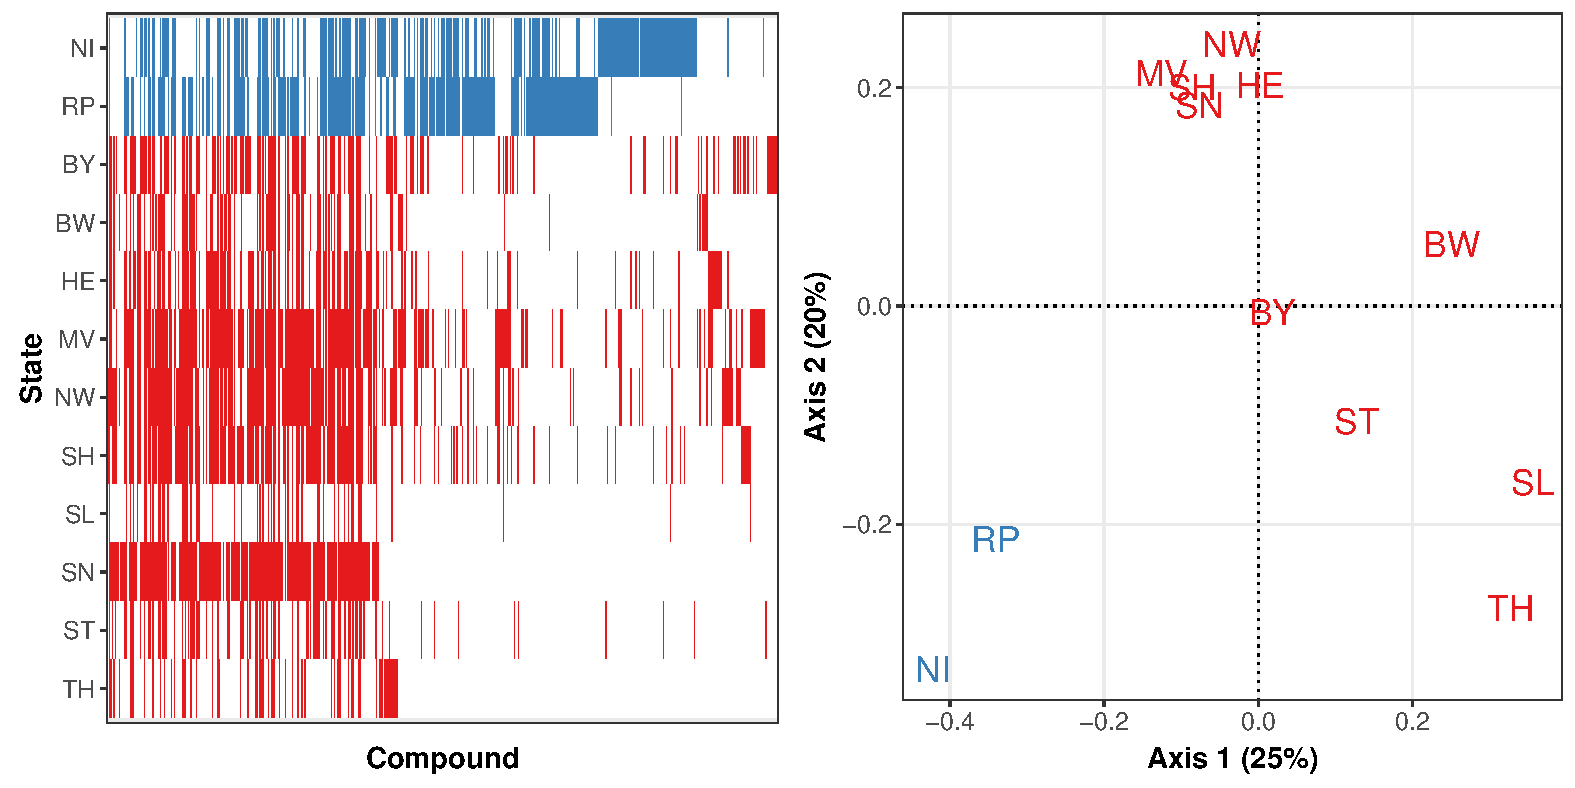
\includegraphics[width=\textwidth]{figs/spectra.pdf}
\end{frame}



\begin{frame}
\frametitle{Mixtures are common, but one compound dominates the risk}
	\begin{columns}
	    \column{.49\textwidth}
	    	\vspace{0.5cm}
	    	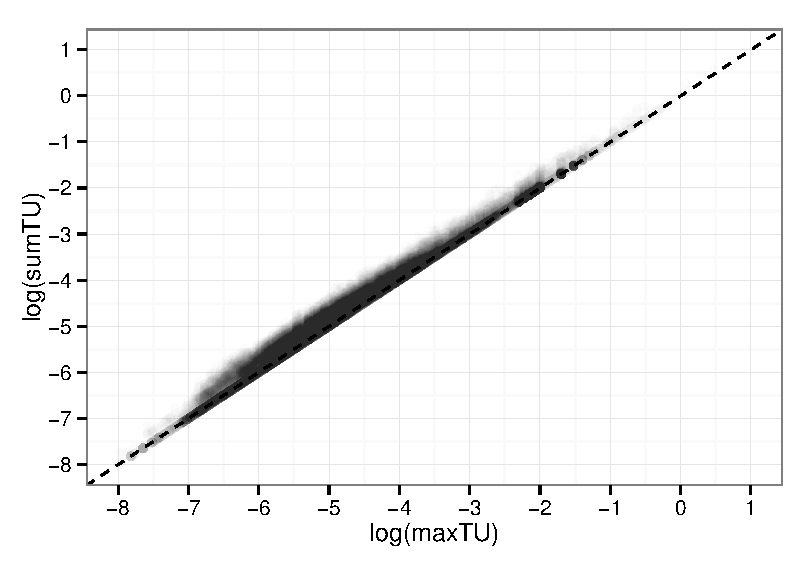
\includegraphics[width=1.2\textwidth, keepaspectratio]{figs/tusum_tumax.pdf}
	    \column{.49\textwidth}
	        \begin{itemize}
	        	\item up to 50 compounds in one sample
	        	\item high correlation
	        	\item $\sim$ 0.5 TU increase 
	        	\item mainly one compound responsible for risk
	        \end{itemize}
	\end{columns}
\end{frame}


\begin{frame}
\frametitle{Implications for National Monitoring}
	\begin{itemize}
    	\item Harmonize between states
	    	\begin{itemize}
		    	\item No. and distribution of sites
		    	\item Spectrum and quality of chemical analysis
		    	\item National Repository for data (see U.S. WQP)
		    \end{itemize}
	    \item Include small water bodies
		    \begin{itemize}
		    	\item streams
		    	\item standing waters
		    \end{itemize}
		\item sampling scheme
			\begin{itemize}
		    	\item event driven sampling
		    	\item automated / passive samplers
		    \end{itemize}
		\item reference sites
			\begin{itemize}
		    	\item no agriculture in catchment
		    \end{itemize}
    \end{itemize}
\end{frame}





\begin{frame}
\frametitle{Implications for Ecological Risk Assessment}
	\begin{itemize}
    	\item Update statistical procedures
    	\item Reproducible and open assessments
    	\item Ban NOEC
    	\item Improve experimental designs
    	\item Revise conclusions on neonicotinoids
    	\item Improvements of the authorisation procedure
    \end{itemize}
\end{frame}


{%
\setbeamertemplate{frame footer}{\scriptsize Modified from: Stehle, Schulz (2015). Agricultural insecticides threaten surface waters at the global scale. PNAS 112, 5750–5755.
}
\begin{frame}
\frametitle{Effects of RAC exceedances}
			\begin{itemize}
				\item RACs should never be exceeded (=protection goal)
				\item If so, biological effects are likely:
			\end{itemize}
	    	    	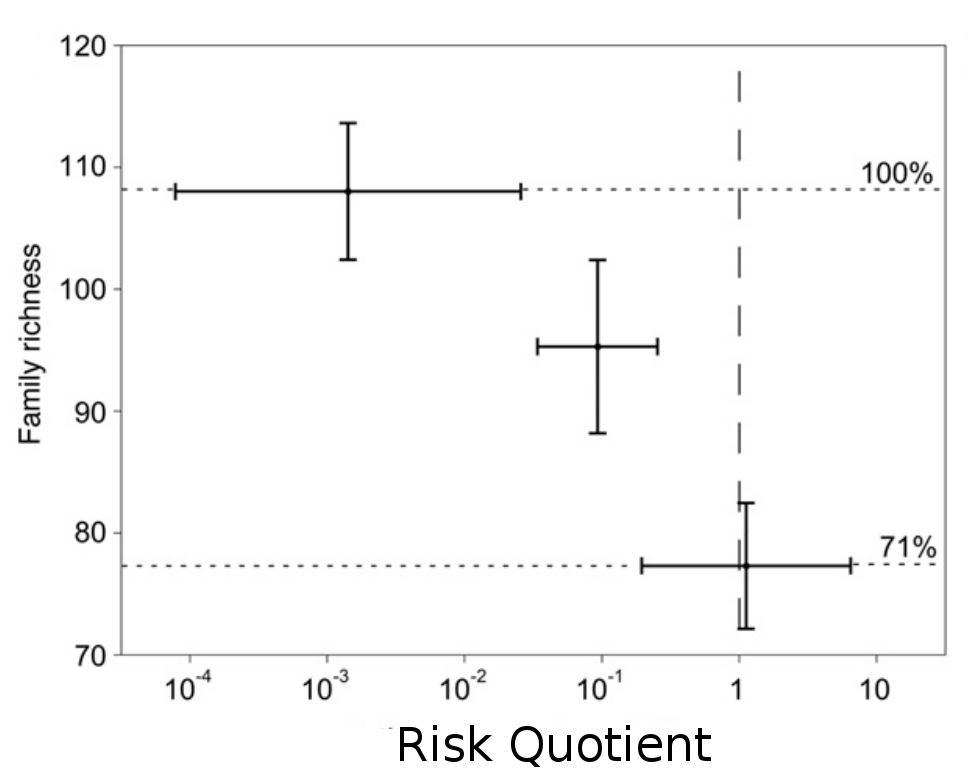
\includegraphics[height=0.7\textheight]{figs/stehle_pnas_2015_mod.png}
\end{frame}
}



\begin{frame}
\frametitle{Reasons for observed RAC exceedances}
	\begin{itemize}
		\item Risk Mitigation fails
			\begin{itemize}
				\item Risk mitigation measures (erosion rills, wind)
				\item Farmer do not adhere (GAP, no spray zones)
			\end{itemize}
		\item Risk Assessment fails
			\begin{itemize}
				\item Exposure Assessment
					\begin{itemize}
						\item Models not working (Knäbel et al.)
					\end{itemize}
				\item Effect Assessment
					\begin{itemize}
						\item Missed sensitive species
						\item New document asks also for insects
					\end{itemize}
			\end{itemize}

	\end{itemize}
\end{frame}



{
\setbeamertemplate{frame footer}{Morrissey et al. (2015). Neonicotinoid contamination of global surface waters and associated risk to aquatic invertebrates: A review. Environment International 74, 291–303.
}
\begin{frame}
\frametitle{Toxicity of Neonicotinoid insecticides}
	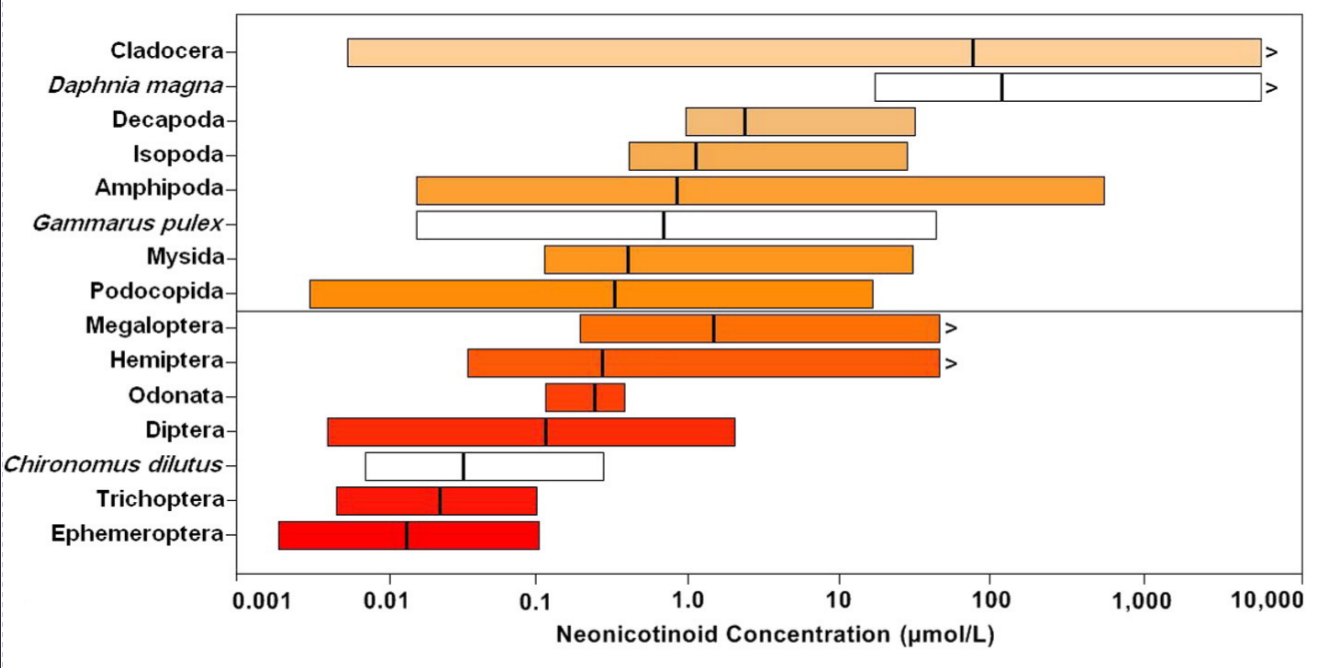
\includegraphics[width = 0.85\textwidth]{figs/morrissey.png}
	\begin{itemize}
			\item \footnotesize EFSA conclusion Imidacloprid 2008:
			\begin{itemize}
				\item \footnotesize Mesocosm NOEC: $0.6~\mu g/L$ (Chiro + Baetidae), AF = 2
				\item \footnotesize "It was not possible to draw a clear conclusion [...] since [Baetidae] were present in too low abundances to allow a reliable statistical  evaluation [...]"
			\end{itemize}
	\end{itemize}
\end{frame}
}



{%
\setbeamertemplate{frame footer}{\scriptsize Bereswill, Streloke, Schulz (2014). Risk mitigation measures for diffuse pesticide entry into aquatic ecosystems: Proposal of a guide to identify appropriate measures on a catchment scale: Guide to Identify Pesticide Risk Mitigation Measures. IEAM 10, 286–298. 
}
\begin{frame}
\frametitle{Risk Mitigation Measures}
	    	    	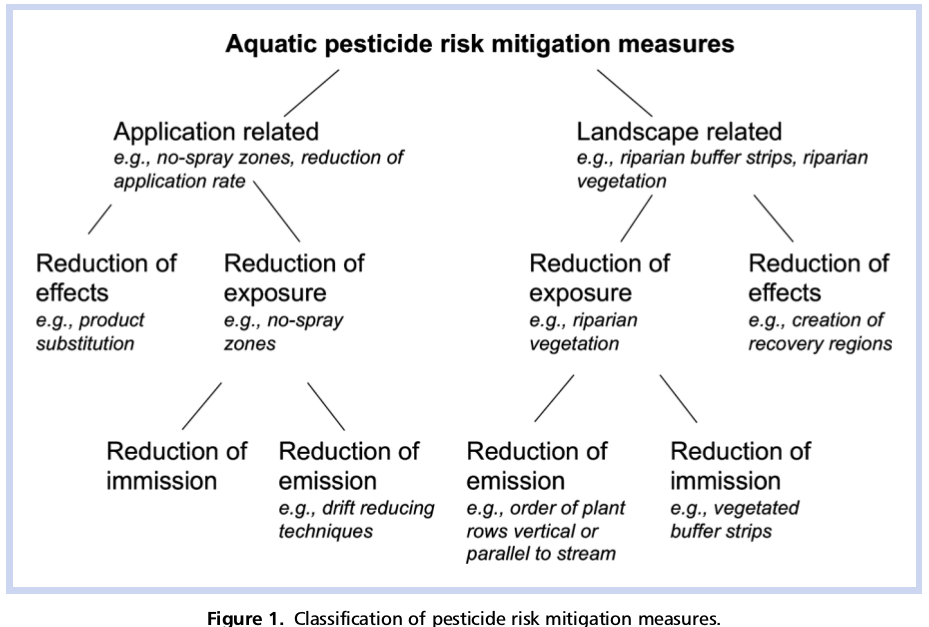
\includegraphics[height=0.8\textheight]{figs/bereswill_2014_fig1.png}
\end{frame}
}





\begin{frame}
\frametitle{Biotic field effects}
	\begin{columns}
	    \column{.49\textwidth}
	    	    	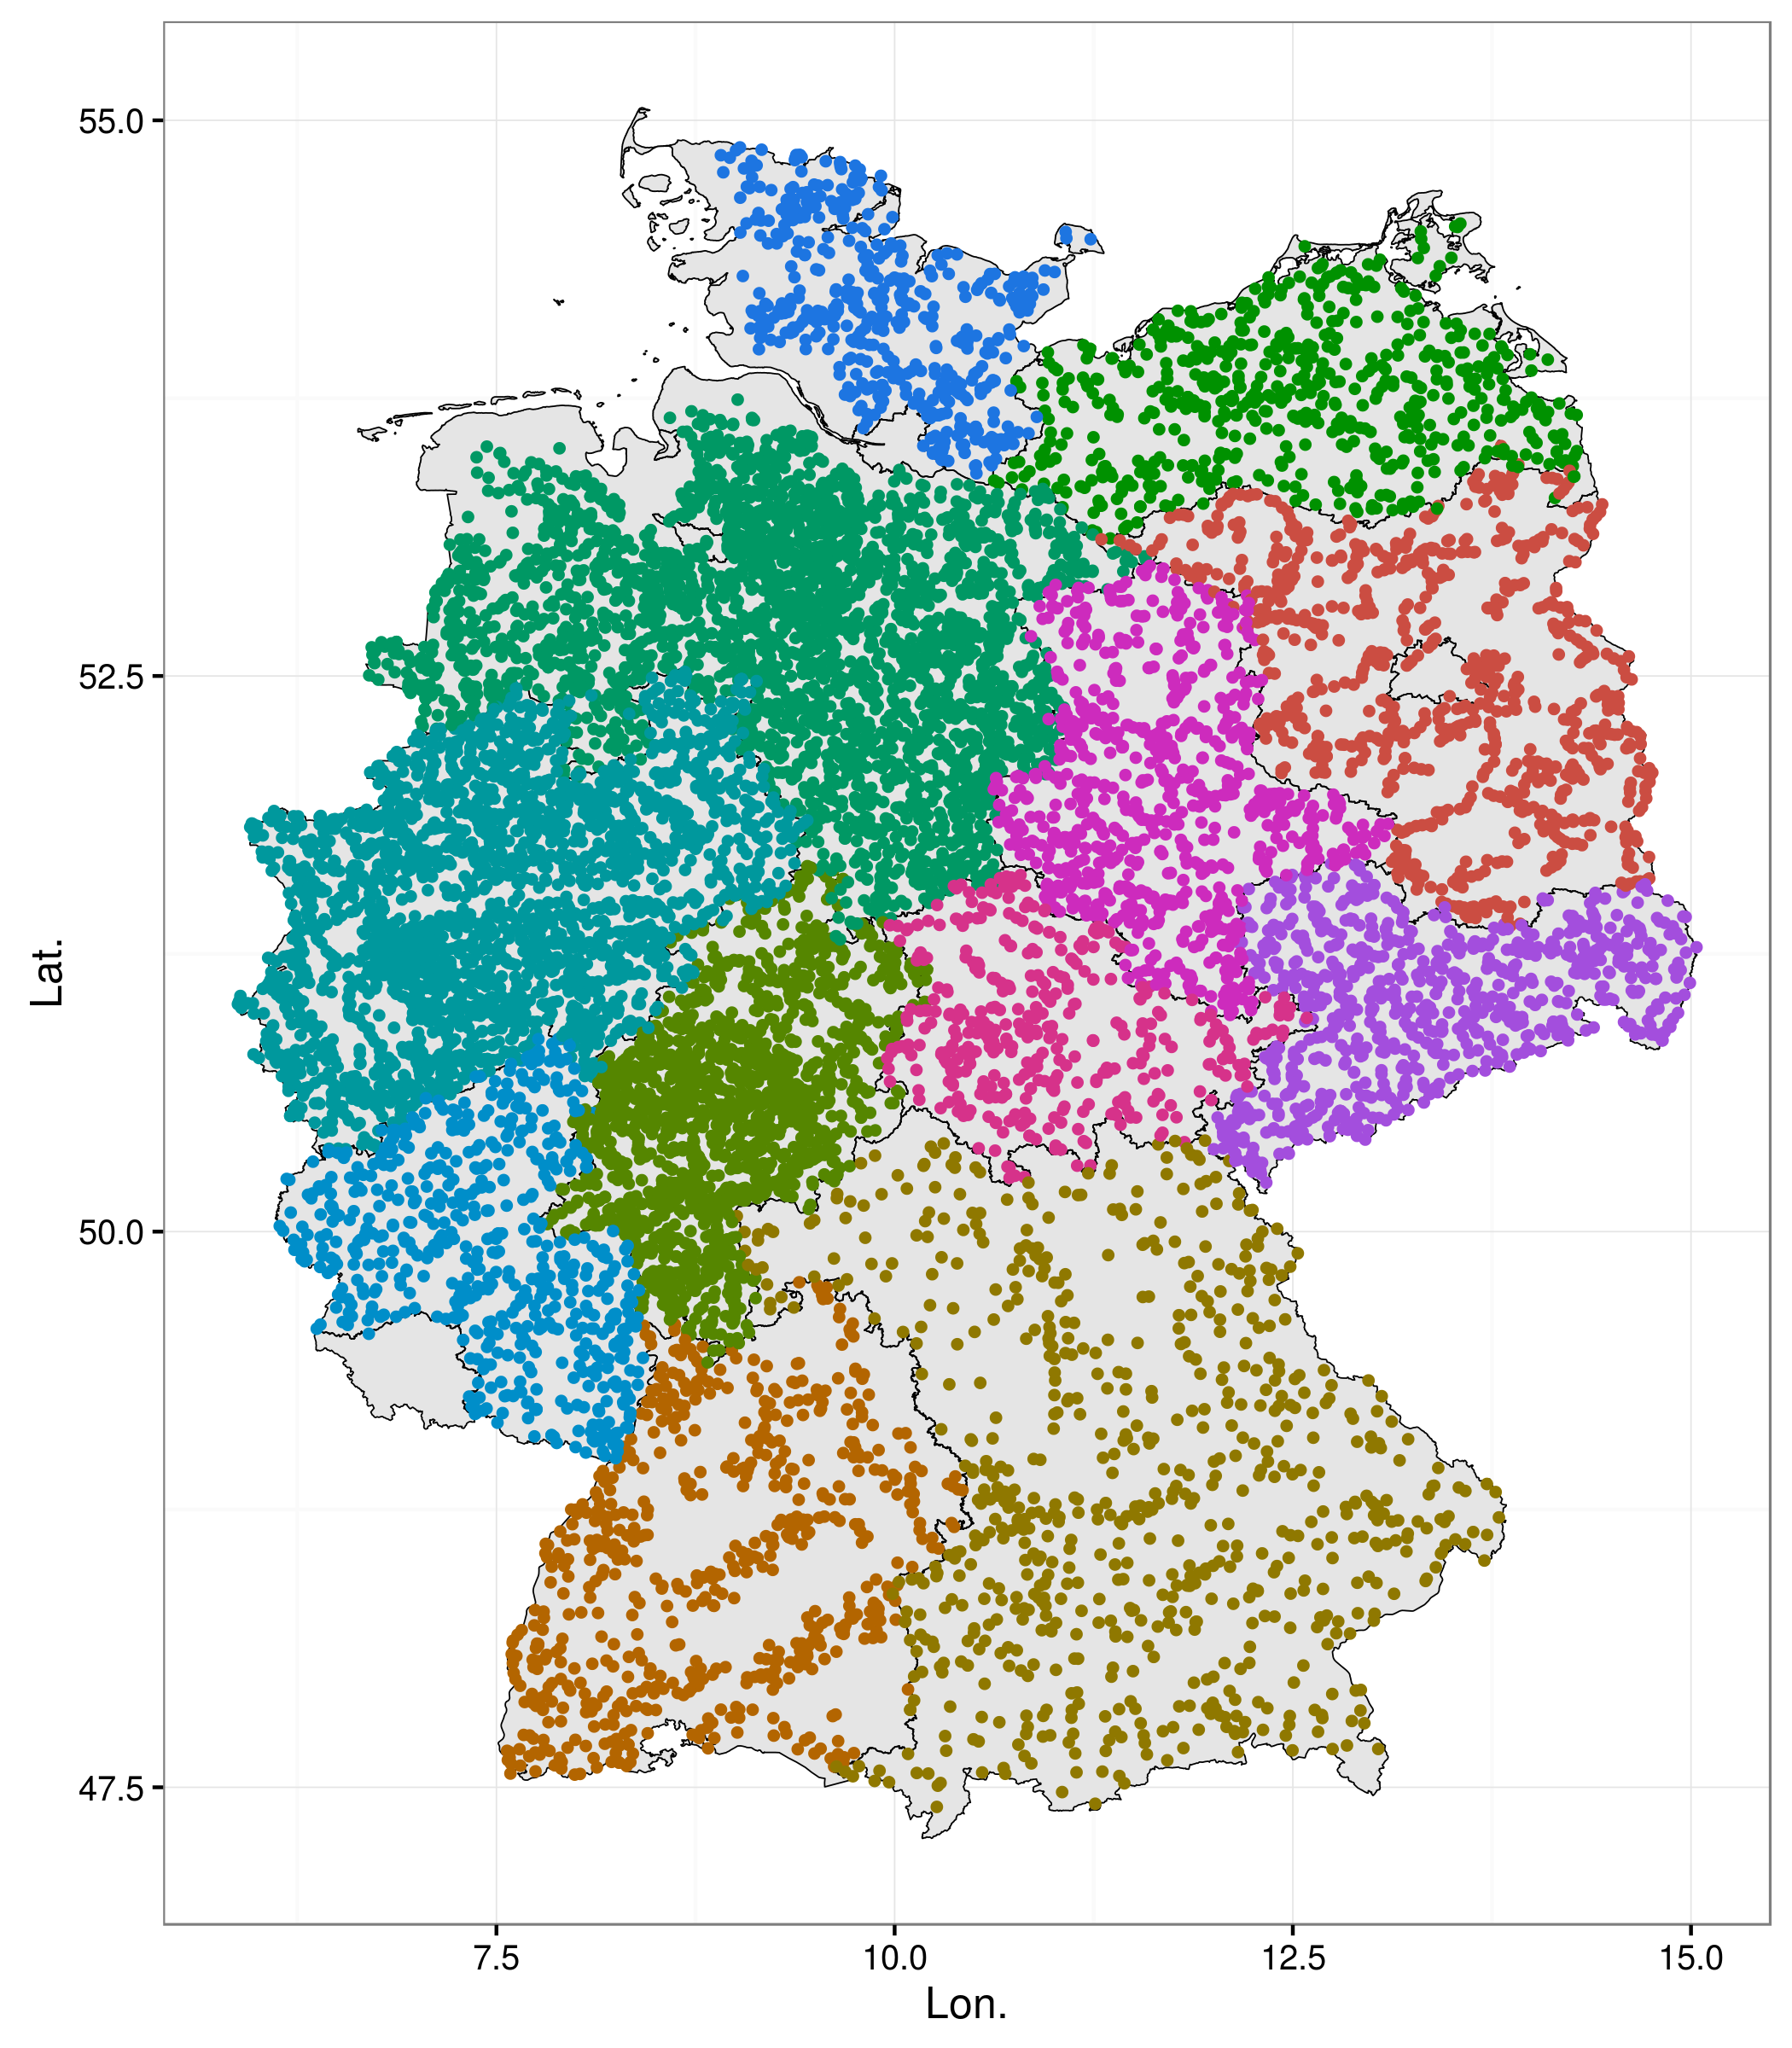
\includegraphics[width=1.1\textwidth, keepaspectratio]{figs/mzb_map.png}
	    \column{.49\textwidth}
	    \begingroup
		\footnotesize % = 10pt in 12pt default
	        \begin{itemize}
	        	\item biological data with good spatial coverage
	        	\item 60\% of spatial congruence 
	        	\item Large scale effects largely unknown.
	        	\item Some work left...
	        	\item Future....
	        \end{itemize}
	       \endgroup
	\end{columns}

\end{frame}


{%
\setbeamertemplate{frame footer}{\scriptsize Source code to retrieve data and reproduce results: \url{http://uni-ko-ld.de/g7}
	}
\begin{frame}
\frametitle{A global perspective (I)}
\begingroup
\footnotesize % = 10pt in 12pt default
	\begin{adjustbox}{max totalsize={\textwidth}{0.90\textheight}}
				% Created by tikzDevice version 0.10.1 on 2016-12-20 15:18:24
% !TEX encoding = UTF-8 Unicode
\begin{tikzpicture}[x=1pt,y=1pt]
\definecolor{fillColor}{RGB}{255,255,255}
\path[use as bounding box,fill=fillColor,fill opacity=0.00] (0,0) rectangle (1011.78,867.24);
\begin{scope}
\path[clip] (  3.50,435.37) rectangle (507.64,867.24);
\definecolor{drawColor}{RGB}{255,255,255}
\definecolor{fillColor}{RGB}{255,255,255}

\path[draw=drawColor,line width= 0.6pt,line join=round,line cap=round,fill=fillColor] (  3.50,435.37) rectangle (507.64,867.24);
\end{scope}
\begin{scope}
\path[clip] ( 84.28,482.41) rectangle (499.64,816.58);
\definecolor{fillColor}{RGB}{255,255,255}

\path[fill=fillColor] ( 84.28,482.41) rectangle (499.64,816.58);
\definecolor{drawColor}{gray}{0.90}

\path[draw=drawColor,line width= 0.6pt,line join=round] ( 84.28,497.60) --
	(499.64,497.60);

\path[draw=drawColor,line width= 0.6pt,line join=round] ( 84.28,539.18) --
	(499.64,539.18);

\path[draw=drawColor,line width= 0.6pt,line join=round] ( 84.28,580.75) --
	(499.64,580.75);

\path[draw=drawColor,line width= 0.6pt,line join=round] ( 84.28,622.33) --
	(499.64,622.33);

\path[draw=drawColor,line width= 0.6pt,line join=round] ( 84.28,663.91) --
	(499.64,663.91);

\path[draw=drawColor,line width= 0.6pt,line join=round] ( 84.28,705.49) --
	(499.64,705.49);

\path[draw=drawColor,line width= 0.6pt,line join=round] ( 84.28,747.07) --
	(499.64,747.07);

\path[draw=drawColor,line width= 0.6pt,line join=round] ( 84.28,788.65) --
	(499.64,788.65);

\path[draw=drawColor,line width= 0.6pt,line join=round] (103.16,482.41) --
	(103.16,816.58);

\path[draw=drawColor,line width= 0.6pt,line join=round] (171.82,482.41) --
	(171.82,816.58);

\path[draw=drawColor,line width= 0.6pt,line join=round] (240.47,482.41) --
	(240.47,816.58);

\path[draw=drawColor,line width= 0.6pt,line join=round] (309.12,482.41) --
	(309.12,816.58);

\path[draw=drawColor,line width= 0.6pt,line join=round] (377.78,482.41) --
	(377.78,816.58);

\path[draw=drawColor,line width= 0.6pt,line join=round] (446.43,482.41) --
	(446.43,816.58);
\definecolor{fillColor}{RGB}{27,158,119}

\path[fill=fillColor,fill opacity=0.80] (103.16,623.07) --
	(110.03,624.76) --
	(116.89,626.95) --
	(123.76,629.62) --
	(130.62,632.33) --
	(137.49,635.08) --
	(144.35,637.97) --
	(151.22,640.84) --
	(158.09,643.74) --
	(164.95,646.81) --
	(171.82,649.92) --
	(178.68,653.12) --
	(185.55,656.30) --
	(192.41,659.43) --
	(199.28,662.60) --
	(206.14,665.69) --
	(213.01,668.70) --
	(219.87,671.70) --
	(226.74,674.76) --
	(233.61,677.88) --
	(240.47,681.03) --
	(247.34,684.26) --
	(254.20,687.60) --
	(261.07,690.98) --
	(267.93,694.35) --
	(274.80,697.79) --
	(281.66,701.35) --
	(288.53,705.00) --
	(295.39,708.69) --
	(302.26,712.37) --
	(309.12,716.02) --
	(315.99,719.62) --
	(322.86,723.08) --
	(329.72,726.57) --
	(336.59,730.02) --
	(343.45,733.53) --
	(350.32,736.96) --
	(357.18,740.40) --
	(364.05,743.80) --
	(370.91,747.17) --
	(377.78,750.51) --
	(384.64,753.84) --
	(391.51,757.12) --
	(398.38,760.41) --
	(405.24,763.72) --
	(412.11,767.05) --
	(418.97,770.40) --
	(425.84,773.76) --
	(432.70,777.19) --
	(439.57,780.62) --
	(446.43,784.05) --
	(453.30,787.51) --
	(460.16,790.73) --
	(467.03,794.32) --
	(473.89,797.83) --
	(480.76,801.39) --
	(480.76,753.00) --
	(473.89,749.72) --
	(467.03,746.44) --
	(460.16,743.19) --
	(453.30,740.18) --
	(446.43,737.01) --
	(439.57,733.89) --
	(432.70,730.80) --
	(425.84,727.76) --
	(418.97,724.76) --
	(412.11,721.75) --
	(405.24,718.74) --
	(398.38,715.74) --
	(391.51,712.75) --
	(384.64,709.76) --
	(377.78,706.74) --
	(370.91,703.68) --
	(364.05,700.59) --
	(357.18,697.46) --
	(350.32,694.31) --
	(343.45,691.16) --
	(336.59,688.01) --
	(329.72,684.85) --
	(322.86,681.69) --
	(315.99,678.48) --
	(309.12,675.20) --
	(302.26,671.87) --
	(295.39,668.47) --
	(288.53,665.06) --
	(281.66,661.68) --
	(274.80,658.39) --
	(267.93,655.20) --
	(261.07,652.09) --
	(254.20,648.98) --
	(247.34,645.92) --
	(240.47,643.00) --
	(233.61,640.15) --
	(226.74,637.34) --
	(219.87,634.59) --
	(213.01,631.89) --
	(206.14,629.16) --
	(199.28,626.42) --
	(192.41,623.62) --
	(185.55,620.80) --
	(178.68,617.98) --
	(171.82,615.13) --
	(164.95,612.35) --
	(158.09,609.63) --
	(151.22,607.03) --
	(144.35,604.49) --
	(137.49,601.96) --
	(130.62,599.58) --
	(123.76,597.27) --
	(116.89,594.98) --
	(110.03,593.20) --
	(103.16,591.97) --
	cycle;
\definecolor{fillColor}{RGB}{217,95,2}

\path[fill=fillColor,fill opacity=0.80] (103.16,591.97) --
	(110.03,593.20) --
	(116.89,594.98) --
	(123.76,597.27) --
	(130.62,599.58) --
	(137.49,601.96) --
	(144.35,604.49) --
	(151.22,607.03) --
	(158.09,609.63) --
	(164.95,612.35) --
	(171.82,615.13) --
	(178.68,617.98) --
	(185.55,620.80) --
	(192.41,623.62) --
	(199.28,626.42) --
	(206.14,629.16) --
	(213.01,631.89) --
	(219.87,634.59) --
	(226.74,637.34) --
	(233.61,640.15) --
	(240.47,643.00) --
	(247.34,645.92) --
	(254.20,648.98) --
	(261.07,652.09) --
	(267.93,655.20) --
	(274.80,658.39) --
	(281.66,661.68) --
	(288.53,665.06) --
	(295.39,668.47) --
	(302.26,671.87) --
	(309.12,675.20) --
	(315.99,678.48) --
	(322.86,681.69) --
	(329.72,684.85) --
	(336.59,688.01) --
	(343.45,691.16) --
	(350.32,694.31) --
	(357.18,697.46) --
	(364.05,700.59) --
	(370.91,703.68) --
	(377.78,706.74) --
	(384.64,709.76) --
	(391.51,712.75) --
	(398.38,715.74) --
	(405.24,718.74) --
	(412.11,721.75) --
	(418.97,724.76) --
	(425.84,727.76) --
	(432.70,730.80) --
	(439.57,733.89) --
	(446.43,737.01) --
	(453.30,740.18) --
	(460.16,743.19) --
	(467.03,746.44) --
	(473.89,749.72) --
	(480.76,753.00) --
	(480.76,645.45) --
	(473.89,643.00) --
	(467.03,640.58) --
	(460.16,638.19) --
	(453.30,636.01) --
	(446.43,633.65) --
	(439.57,631.31) --
	(432.70,629.00) --
	(425.84,626.72) --
	(418.97,624.46) --
	(412.11,622.21) --
	(405.24,619.99) --
	(398.38,617.77) --
	(391.51,615.58) --
	(384.64,613.40) --
	(377.78,611.24) --
	(370.91,609.10) --
	(364.05,606.97) --
	(357.18,604.86) --
	(350.32,602.74) --
	(343.45,600.63) --
	(336.59,598.52) --
	(329.72,596.42) --
	(322.86,594.32) --
	(315.99,592.21) --
	(309.12,590.13) --
	(302.26,588.07) --
	(295.39,586.01) --
	(288.53,583.97) --
	(281.66,581.97) --
	(274.80,579.99) --
	(267.93,578.05) --
	(261.07,576.15) --
	(254.20,574.29) --
	(247.34,572.48) --
	(240.47,570.71) --
	(233.61,568.97) --
	(226.74,567.28) --
	(219.87,565.64) --
	(213.01,564.04) --
	(206.14,562.48) --
	(199.28,560.96) --
	(192.41,559.48) --
	(185.55,558.03) --
	(178.68,556.62) --
	(171.82,555.25) --
	(164.95,553.91) --
	(158.09,552.60) --
	(151.22,551.32) --
	(144.35,550.08) --
	(137.49,548.88) --
	(130.62,547.71) --
	(123.76,546.57) --
	(116.89,545.48) --
	(110.03,544.41) --
	(103.16,543.38) --
	cycle;
\definecolor{fillColor}{RGB}{117,112,179}

\path[fill=fillColor,fill opacity=0.80] (103.16,543.38) --
	(110.03,544.41) --
	(116.89,545.48) --
	(123.76,546.57) --
	(130.62,547.71) --
	(137.49,548.88) --
	(144.35,550.08) --
	(151.22,551.32) --
	(158.09,552.60) --
	(164.95,553.91) --
	(171.82,555.25) --
	(178.68,556.62) --
	(185.55,558.03) --
	(192.41,559.48) --
	(199.28,560.96) --
	(206.14,562.48) --
	(213.01,564.04) --
	(219.87,565.64) --
	(226.74,567.28) --
	(233.61,568.97) --
	(240.47,570.71) --
	(247.34,572.48) --
	(254.20,574.29) --
	(261.07,576.15) --
	(267.93,578.05) --
	(274.80,579.99) --
	(281.66,581.97) --
	(288.53,583.97) --
	(295.39,586.01) --
	(302.26,588.07) --
	(309.12,590.13) --
	(315.99,592.21) --
	(322.86,594.32) --
	(329.72,596.42) --
	(336.59,598.52) --
	(343.45,600.63) --
	(350.32,602.74) --
	(357.18,604.86) --
	(364.05,606.97) --
	(370.91,609.10) --
	(377.78,611.24) --
	(384.64,613.40) --
	(391.51,615.58) --
	(398.38,617.77) --
	(405.24,619.99) --
	(412.11,622.21) --
	(418.97,624.46) --
	(425.84,626.72) --
	(432.70,629.00) --
	(439.57,631.31) --
	(446.43,633.65) --
	(453.30,636.01) --
	(460.16,638.19) --
	(467.03,640.58) --
	(473.89,643.00) --
	(480.76,645.45) --
	(480.76,523.92) --
	(473.89,523.22) --
	(467.03,522.53) --
	(460.16,521.86) --
	(453.30,521.40) --
	(446.43,520.75) --
	(439.57,520.13) --
	(432.70,519.53) --
	(425.84,518.94) --
	(418.97,518.37) --
	(412.11,517.81) --
	(405.24,517.26) --
	(398.38,516.73) --
	(391.51,516.20) --
	(384.64,515.70) --
	(377.78,515.21) --
	(370.91,514.74) --
	(364.05,514.29) --
	(357.18,513.85) --
	(350.32,513.42) --
	(343.45,513.00) --
	(336.59,512.58) --
	(329.72,512.16) --
	(322.86,511.75) --
	(315.99,511.35) --
	(309.12,510.97) --
	(302.26,510.61) --
	(295.39,510.26) --
	(288.53,509.93) --
	(281.66,509.62) --
	(274.80,509.32) --
	(267.93,509.04) --
	(261.07,508.77) --
	(254.20,508.51) --
	(247.34,508.26) --
	(240.47,508.01) --
	(233.61,507.77) --
	(226.74,507.53) --
	(219.87,507.29) --
	(213.01,507.05) --
	(206.14,506.82) --
	(199.28,506.60) --
	(192.41,506.38) --
	(185.55,506.16) --
	(178.68,505.95) --
	(171.82,505.74) --
	(164.95,505.53) --
	(158.09,505.34) --
	(151.22,505.14) --
	(144.35,504.96) --
	(137.49,504.78) --
	(130.62,504.62) --
	(123.76,504.46) --
	(116.89,504.31) --
	(110.03,504.17) --
	(103.16,504.03) --
	cycle;
\definecolor{fillColor}{RGB}{231,41,138}

\path[fill=fillColor,fill opacity=0.80] (103.16,504.03) --
	(110.03,504.17) --
	(116.89,504.31) --
	(123.76,504.46) --
	(130.62,504.62) --
	(137.49,504.78) --
	(144.35,504.96) --
	(151.22,505.14) --
	(158.09,505.34) --
	(164.95,505.53) --
	(171.82,505.74) --
	(178.68,505.95) --
	(185.55,506.16) --
	(192.41,506.38) --
	(199.28,506.60) --
	(206.14,506.82) --
	(213.01,507.05) --
	(219.87,507.29) --
	(226.74,507.53) --
	(233.61,507.77) --
	(240.47,508.01) --
	(247.34,508.26) --
	(254.20,508.51) --
	(261.07,508.77) --
	(267.93,509.04) --
	(274.80,509.32) --
	(281.66,509.62) --
	(288.53,509.93) --
	(295.39,510.26) --
	(302.26,510.61) --
	(309.12,510.97) --
	(315.99,511.35) --
	(322.86,511.75) --
	(329.72,512.16) --
	(336.59,512.58) --
	(343.45,513.00) --
	(350.32,513.42) --
	(357.18,513.85) --
	(364.05,514.29) --
	(370.91,514.74) --
	(377.78,515.21) --
	(384.64,515.70) --
	(391.51,516.20) --
	(398.38,516.73) --
	(405.24,517.26) --
	(412.11,517.81) --
	(418.97,518.37) --
	(425.84,518.94) --
	(432.70,519.53) --
	(439.57,520.13) --
	(446.43,520.75) --
	(453.30,521.40) --
	(460.16,521.86) --
	(467.03,522.53) --
	(473.89,523.22) --
	(480.76,523.92) --
	(480.76,497.60) --
	(473.89,497.60) --
	(467.03,497.60) --
	(460.16,497.60) --
	(453.30,497.60) --
	(446.43,497.60) --
	(439.57,497.60) --
	(432.70,497.60) --
	(425.84,497.60) --
	(418.97,497.60) --
	(412.11,497.60) --
	(405.24,497.60) --
	(398.38,497.60) --
	(391.51,497.60) --
	(384.64,497.60) --
	(377.78,497.60) --
	(370.91,497.60) --
	(364.05,497.60) --
	(357.18,497.60) --
	(350.32,497.60) --
	(343.45,497.60) --
	(336.59,497.60) --
	(329.72,497.60) --
	(322.86,497.60) --
	(315.99,497.60) --
	(309.12,497.60) --
	(302.26,497.60) --
	(295.39,497.60) --
	(288.53,497.60) --
	(281.66,497.60) --
	(274.80,497.60) --
	(267.93,497.60) --
	(261.07,497.60) --
	(254.20,497.60) --
	(247.34,497.60) --
	(240.47,497.60) --
	(233.61,497.60) --
	(226.74,497.60) --
	(219.87,497.60) --
	(213.01,497.60) --
	(206.14,497.60) --
	(199.28,497.60) --
	(192.41,497.60) --
	(185.55,497.60) --
	(178.68,497.60) --
	(171.82,497.60) --
	(164.95,497.60) --
	(158.09,497.60) --
	(151.22,497.60) --
	(144.35,497.60) --
	(137.49,497.60) --
	(130.62,497.60) --
	(123.76,497.60) --
	(116.89,497.60) --
	(110.03,497.60) --
	(103.16,497.60) --
	cycle;
\definecolor{drawColor}{gray}{0.50}

\path[draw=drawColor,line width= 0.6pt,line join=round,line cap=round] ( 84.28,482.41) rectangle (499.64,816.58);
\end{scope}
\begin{scope}
\path[clip] (  0.00,  0.00) rectangle (1011.78,867.24);
\definecolor{drawColor}{gray}{0.30}

\node[text=drawColor,anchor=base east,inner sep=0pt, outer sep=0pt, scale=  1.28] at ( 77.08,488.76) {\bfseries 0e+00};

\node[text=drawColor,anchor=base east,inner sep=0pt, outer sep=0pt, scale=  1.28] at ( 77.08,530.34) {\bfseries 1e+09};

\node[text=drawColor,anchor=base east,inner sep=0pt, outer sep=0pt, scale=  1.28] at ( 77.08,571.92) {\bfseries 2e+09};

\node[text=drawColor,anchor=base east,inner sep=0pt, outer sep=0pt, scale=  1.28] at ( 77.08,613.50) {\bfseries 3e+09};

\node[text=drawColor,anchor=base east,inner sep=0pt, outer sep=0pt, scale=  1.28] at ( 77.08,655.08) {\bfseries 4e+09};

\node[text=drawColor,anchor=base east,inner sep=0pt, outer sep=0pt, scale=  1.28] at ( 77.08,696.66) {\bfseries 5e+09};

\node[text=drawColor,anchor=base east,inner sep=0pt, outer sep=0pt, scale=  1.28] at ( 77.08,738.24) {\bfseries 6e+09};

\node[text=drawColor,anchor=base east,inner sep=0pt, outer sep=0pt, scale=  1.28] at ( 77.08,779.81) {\bfseries 7e+09};
\end{scope}
\begin{scope}
\path[clip] (  0.00,  0.00) rectangle (1011.78,867.24);
\definecolor{drawColor}{RGB}{0,0,0}

\path[draw=drawColor,line width= 0.6pt,line join=round] ( 80.28,497.60) --
	( 84.28,497.60);

\path[draw=drawColor,line width= 0.6pt,line join=round] ( 80.28,539.18) --
	( 84.28,539.18);

\path[draw=drawColor,line width= 0.6pt,line join=round] ( 80.28,580.75) --
	( 84.28,580.75);

\path[draw=drawColor,line width= 0.6pt,line join=round] ( 80.28,622.33) --
	( 84.28,622.33);

\path[draw=drawColor,line width= 0.6pt,line join=round] ( 80.28,663.91) --
	( 84.28,663.91);

\path[draw=drawColor,line width= 0.6pt,line join=round] ( 80.28,705.49) --
	( 84.28,705.49);

\path[draw=drawColor,line width= 0.6pt,line join=round] ( 80.28,747.07) --
	( 84.28,747.07);

\path[draw=drawColor,line width= 0.6pt,line join=round] ( 80.28,788.65) --
	( 84.28,788.65);
\end{scope}
\begin{scope}
\path[clip] (  0.00,  0.00) rectangle (1011.78,867.24);
\definecolor{drawColor}{RGB}{0,0,0}

\path[draw=drawColor,line width= 0.6pt,line join=round] (103.16,478.41) --
	(103.16,482.41);

\path[draw=drawColor,line width= 0.6pt,line join=round] (171.82,478.41) --
	(171.82,482.41);

\path[draw=drawColor,line width= 0.6pt,line join=round] (240.47,478.41) --
	(240.47,482.41);

\path[draw=drawColor,line width= 0.6pt,line join=round] (309.12,478.41) --
	(309.12,482.41);

\path[draw=drawColor,line width= 0.6pt,line join=round] (377.78,478.41) --
	(377.78,482.41);

\path[draw=drawColor,line width= 0.6pt,line join=round] (446.43,478.41) --
	(446.43,482.41);
\end{scope}
\begin{scope}
\path[clip] (  0.00,  0.00) rectangle (1011.78,867.24);
\definecolor{drawColor}{gray}{0.30}

\node[text=drawColor,anchor=base,inner sep=0pt, outer sep=0pt, scale=  1.28] at (103.16,466.37) {\bfseries 1960};

\node[text=drawColor,anchor=base,inner sep=0pt, outer sep=0pt, scale=  1.28] at (171.82,466.37) {\bfseries 1970};

\node[text=drawColor,anchor=base,inner sep=0pt, outer sep=0pt, scale=  1.28] at (240.47,466.37) {\bfseries 1980};

\node[text=drawColor,anchor=base,inner sep=0pt, outer sep=0pt, scale=  1.28] at (309.12,466.37) {\bfseries 1990};

\node[text=drawColor,anchor=base,inner sep=0pt, outer sep=0pt, scale=  1.28] at (377.78,466.37) {\bfseries 2000};

\node[text=drawColor,anchor=base,inner sep=0pt, outer sep=0pt, scale=  1.28] at (446.43,466.37) {\bfseries 2010};
\end{scope}
\begin{scope}
\path[clip] (  0.00,  0.00) rectangle (1011.78,867.24);
\definecolor{drawColor}{RGB}{0,0,0}

\node[text=drawColor,anchor=base,inner sep=0pt, outer sep=0pt, scale=  1.92] at (291.96,446.66) {Year};
\end{scope}
\begin{scope}
\path[clip] (  0.00,  0.00) rectangle (1011.78,867.24);
\definecolor{drawColor}{RGB}{0,0,0}

\node[text=drawColor,rotate= 90.00,anchor=base,inner sep=0pt, outer sep=0pt, scale=  1.92] at ( 29.17,649.49) {Population};
\end{scope}
\begin{scope}
\path[clip] (  0.00,  0.00) rectangle (1011.78,867.24);
\definecolor{drawColor}{RGB}{0,0,0}

\node[text=drawColor,anchor=base west,inner sep=0pt, outer sep=0pt, scale=  1.44] at ( 84.28,824.01) {Source: World Bank};
\end{scope}
\begin{scope}
\path[clip] (  0.00,  0.00) rectangle (1011.78,867.24);
\definecolor{drawColor}{RGB}{0,0,0}

\node[text=drawColor,anchor=base west,inner sep=0pt, outer sep=0pt, scale=  1.92] at ( 84.28,846.02) {Population since 1960};
\end{scope}
\begin{scope}
\path[clip] (507.64,435.37) rectangle (1011.78,867.24);
\definecolor{drawColor}{RGB}{255,255,255}
\definecolor{fillColor}{RGB}{255,255,255}

\path[draw=drawColor,line width= 0.6pt,line join=round,line cap=round,fill=fillColor] (507.64,435.37) rectangle (1011.78,867.24);
\end{scope}
\begin{scope}
\path[clip] (567.92,482.41) rectangle (1003.78,814.31);
\definecolor{fillColor}{RGB}{255,255,255}

\path[fill=fillColor] (567.92,482.41) rectangle (1003.78,814.31);
\definecolor{drawColor}{gray}{0.90}

\path[draw=drawColor,line width= 0.6pt,line join=round] (567.92,558.01) --
	(1003.78,558.01);

\path[draw=drawColor,line width= 0.6pt,line join=round] (567.92,640.62) --
	(1003.78,640.62);

\path[draw=drawColor,line width= 0.6pt,line join=round] (567.92,723.23) --
	(1003.78,723.23);

\path[draw=drawColor,line width= 0.6pt,line join=round] (567.92,805.84) --
	(1003.78,805.84);

\path[draw=drawColor,line width= 0.6pt,line join=round] (580.11,482.41) --
	(580.11,814.31);

\path[draw=drawColor,line width= 0.6pt,line join=round] (656.31,482.41) --
	(656.31,814.31);

\path[draw=drawColor,line width= 0.6pt,line join=round] (732.51,482.41) --
	(732.51,814.31);

\path[draw=drawColor,line width= 0.6pt,line join=round] (808.71,482.41) --
	(808.71,814.31);

\path[draw=drawColor,line width= 0.6pt,line join=round] (884.91,482.41) --
	(884.91,814.31);

\path[draw=drawColor,line width= 0.6pt,line join=round] (961.11,482.41) --
	(961.11,814.31);
\definecolor{drawColor}{RGB}{0,0,0}

\path[draw=drawColor,line width= 2.3pt,line join=round] (587.73,497.49) --
	(595.35,501.11) --
	(602.97,504.83) --
	(610.59,507.47) --
	(618.21,510.11) --
	(625.83,513.14) --
	(633.45,518.07) --
	(641.07,521.08) --
	(648.69,522.33) --
	(656.31,526.22) --
	(663.93,529.87) --
	(671.55,529.94) --
	(679.17,535.69) --
	(686.79,538.93) --
	(694.41,544.07) --
	(702.03,547.30) --
	(709.65,550.87) --
	(717.27,557.80) --
	(724.89,561.82) --
	(732.51,563.90) --
	(740.13,570.46) --
	(747.75,576.29) --
	(755.37,576.01) --
	(762.99,586.23) --
	(770.61,590.81) --
	(778.23,594.06) --
	(785.85,596.11) --
	(793.47,599.61) --
	(801.09,607.61) --
	(808.71,614.64) --
	(816.33,618.03) --
	(823.95,633.79) --
	(831.57,635.89) --
	(839.19,642.67) --
	(846.81,648.34) --
	(854.43,659.42) --
	(862.05,664.26) --
	(869.67,669.58) --
	(877.29,679.55) --
	(884.91,685.50) --
	(892.53,689.11) --
	(900.15,693.80) --
	(907.77,703.44) --
	(915.39,715.27) --
	(923.01,723.12) --
	(930.63,731.28) --
	(938.25,743.26) --
	(945.87,757.11) --
	(953.49,761.47) --
	(961.11,770.61) --
	(968.73,781.97) --
	(976.35,787.94) --
	(983.97,799.23);
\definecolor{drawColor}{gray}{0.50}

\path[draw=drawColor,line width= 0.6pt,line join=round,line cap=round] (567.92,482.41) rectangle (1003.78,814.31);
\end{scope}
\begin{scope}
\path[clip] (  0.00,  0.00) rectangle (1011.78,867.24);
\definecolor{drawColor}{gray}{0.30}

\node[text=drawColor,anchor=base east,inner sep=0pt, outer sep=0pt, scale=  1.28] at (560.72,549.18) {\bfseries 50};

\node[text=drawColor,anchor=base east,inner sep=0pt, outer sep=0pt, scale=  1.28] at (560.72,631.79) {\bfseries 75};

\node[text=drawColor,anchor=base east,inner sep=0pt, outer sep=0pt, scale=  1.28] at (560.72,714.40) {\bfseries 100};

\node[text=drawColor,anchor=base east,inner sep=0pt, outer sep=0pt, scale=  1.28] at (560.72,797.01) {\bfseries 125};
\end{scope}
\begin{scope}
\path[clip] (  0.00,  0.00) rectangle (1011.78,867.24);
\definecolor{drawColor}{RGB}{0,0,0}

\path[draw=drawColor,line width= 0.6pt,line join=round] (563.92,558.01) --
	(567.92,558.01);

\path[draw=drawColor,line width= 0.6pt,line join=round] (563.92,640.62) --
	(567.92,640.62);

\path[draw=drawColor,line width= 0.6pt,line join=round] (563.92,723.23) --
	(567.92,723.23);

\path[draw=drawColor,line width= 0.6pt,line join=round] (563.92,805.84) --
	(567.92,805.84);
\end{scope}
\begin{scope}
\path[clip] (  0.00,  0.00) rectangle (1011.78,867.24);
\definecolor{drawColor}{RGB}{0,0,0}

\path[draw=drawColor,line width= 0.6pt,line join=round] (580.11,478.41) --
	(580.11,482.41);

\path[draw=drawColor,line width= 0.6pt,line join=round] (656.31,478.41) --
	(656.31,482.41);

\path[draw=drawColor,line width= 0.6pt,line join=round] (732.51,478.41) --
	(732.51,482.41);

\path[draw=drawColor,line width= 0.6pt,line join=round] (808.71,478.41) --
	(808.71,482.41);

\path[draw=drawColor,line width= 0.6pt,line join=round] (884.91,478.41) --
	(884.91,482.41);

\path[draw=drawColor,line width= 0.6pt,line join=round] (961.11,478.41) --
	(961.11,482.41);
\end{scope}
\begin{scope}
\path[clip] (  0.00,  0.00) rectangle (1011.78,867.24);
\definecolor{drawColor}{gray}{0.30}

\node[text=drawColor,anchor=base,inner sep=0pt, outer sep=0pt, scale=  1.28] at (580.11,466.37) {\bfseries 1960};

\node[text=drawColor,anchor=base,inner sep=0pt, outer sep=0pt, scale=  1.28] at (656.31,466.37) {\bfseries 1970};

\node[text=drawColor,anchor=base,inner sep=0pt, outer sep=0pt, scale=  1.28] at (732.51,466.37) {\bfseries 1980};

\node[text=drawColor,anchor=base,inner sep=0pt, outer sep=0pt, scale=  1.28] at (808.71,466.37) {\bfseries 1990};

\node[text=drawColor,anchor=base,inner sep=0pt, outer sep=0pt, scale=  1.28] at (884.91,466.37) {\bfseries 2000};

\node[text=drawColor,anchor=base,inner sep=0pt, outer sep=0pt, scale=  1.28] at (961.11,466.37) {\bfseries 2010};
\end{scope}
\begin{scope}
\path[clip] (  0.00,  0.00) rectangle (1011.78,867.24);
\definecolor{drawColor}{RGB}{0,0,0}

\node[text=drawColor,anchor=base,inner sep=0pt, outer sep=0pt, scale=  1.92] at (785.85,446.66) {Year};
\end{scope}
\begin{scope}
\path[clip] (  0.00,  0.00) rectangle (1011.78,867.24);
\definecolor{drawColor}{RGB}{0,0,0}

\node[text=drawColor,rotate= 90.00,anchor=base,inner sep=0pt, outer sep=0pt, scale=  1.92] at (532.15,648.36) {Index value};
\end{scope}
\begin{scope}
\path[clip] (  0.00,  0.00) rectangle (1011.78,867.24);
\definecolor{drawColor}{RGB}{0,0,0}

\node[text=drawColor,anchor=base west,inner sep=0pt, outer sep=0pt, scale=  1.44] at (567.92,824.01) {Source: World Bank; (2004-2006 = 100)};
\end{scope}
\begin{scope}
\path[clip] (  0.00,  0.00) rectangle (1011.78,867.24);
\definecolor{drawColor}{RGB}{0,0,0}

\node[text=drawColor,anchor=base west,inner sep=0pt, outer sep=0pt, scale=  1.92] at (567.92,846.02) {Food production index};
\end{scope}
\begin{scope}
\path[clip] (  3.50,  3.50) rectangle (507.64,435.37);
\definecolor{drawColor}{RGB}{255,255,255}
\definecolor{fillColor}{RGB}{255,255,255}

\path[draw=drawColor,line width= 0.6pt,line join=round,line cap=round,fill=fillColor] (  3.50,  3.50) rectangle (507.64,435.37);
\end{scope}
\begin{scope}
\path[clip] ( 58.89, 50.54) rectangle (499.64,384.55);
\definecolor{fillColor}{RGB}{255,255,255}

\path[fill=fillColor] ( 58.89, 50.54) rectangle (499.64,384.55);
\definecolor{drawColor}{gray}{0.90}

\path[draw=drawColor,line width= 0.6pt,line join=round] ( 58.89,119.66) --
	(499.64,119.66);

\path[draw=drawColor,line width= 0.6pt,line join=round] ( 58.89,189.49) --
	(499.64,189.49);

\path[draw=drawColor,line width= 0.6pt,line join=round] ( 58.89,259.32) --
	(499.64,259.32);

\path[draw=drawColor,line width= 0.6pt,line join=round] ( 58.89,329.15) --
	(499.64,329.15);

\path[draw=drawColor,line width= 0.6pt,line join=round] ( 71.22, 50.54) --
	( 71.22,384.55);

\path[draw=drawColor,line width= 0.6pt,line join=round] (148.27, 50.54) --
	(148.27,384.55);

\path[draw=drawColor,line width= 0.6pt,line join=round] (225.33, 50.54) --
	(225.33,384.55);

\path[draw=drawColor,line width= 0.6pt,line join=round] (302.38, 50.54) --
	(302.38,384.55);

\path[draw=drawColor,line width= 0.6pt,line join=round] (379.44, 50.54) --
	(379.44,384.55);

\path[draw=drawColor,line width= 0.6pt,line join=round] (456.49, 50.54) --
	(456.49,384.55);
\definecolor{drawColor}{RGB}{27,158,119}

\path[draw=drawColor,line width= 2.3pt,line join=round] ( 78.92,297.38) --
	( 86.63,296.77) --
	( 94.33,296.70) --
	(102.04,296.56) --
	(109.75,296.62) --
	(117.45,296.82) --
	(125.16,297.56) --
	(132.86,296.47) --
	(140.57,297.68) --
	(148.27,297.45) --
	(155.98,296.62) --
	(163.68,296.61) --
	(171.39,296.96) --
	(179.09,296.73) --
	(186.80,296.38) --
	(194.51,296.75) --
	(202.21,292.75) --
	(209.92,290.86) --
	(217.62,291.96) --
	(225.33,292.53) --
	(233.03,292.25) --
	(240.74,291.43) --
	(248.44,288.36) --
	(256.15,291.17) --
	(263.85,293.07) --
	(271.56,294.28) --
	(279.26,294.38) --
	(286.97,296.64) --
	(294.68,296.49) --
	(302.38,297.17) --
	(310.09,295.22) --
	(317.79,295.37) --
	(325.50,311.63) --
	(333.20,314.03) --
	(340.91,310.76) --
	(348.61,309.83) --
	(356.32,306.81) --
	(364.02,307.22) --
	(371.73,302.60) --
	(379.44,303.26) --
	(387.14,302.87) --
	(394.85,296.95) --
	(402.55,293.58) --
	(410.26,292.97) --
	(417.96,294.80) --
	(425.67,288.50) --
	(433.37,285.18) --
	(441.08,282.12) --
	(448.78,276.70) --
	(456.49,270.65) --
	(464.20,273.02) --
	(471.90,273.63) --
	(479.61,268.58);
\definecolor{drawColor}{RGB}{217,95,2}

\path[draw=drawColor,line width= 2.3pt,line join=round] ( 78.92,310.81) --
	( 86.63,312.74) --
	( 94.33,314.44) --
	(102.04,316.42) --
	(109.75,318.91) --
	(117.45,317.81) --
	(125.16,319.73) --
	(132.86,320.08) --
	(140.57,322.84) --
	(148.27,321.88) --
	(155.98,321.10) --
	(163.68,319.50) --
	(171.39,324.31) --
	(179.09,322.61) --
	(186.80,323.37) --
	(194.51,314.44) --
	(202.21,313.00) --
	(209.92,313.33) --
	(217.62,312.33) --
	(225.33,314.97) --
	(233.03,313.09) --
	(240.74,315.83) --
	(248.44,315.08) --
	(256.15,319.45) --
	(263.85,324.66) --
	(271.56,330.63) --
	(279.26,335.40) --
	(286.97,338.38) --
	(294.68,342.03) --
	(302.38,342.56) --
	(310.09,343.16) --
	(317.79,342.99) --
	(325.50,344.14) --
	(333.20,346.36) --
	(340.91,349.89) --
	(348.61,350.98) --
	(356.32,359.75) --
	(364.02,361.38) --
	(371.73,365.51) --
	(379.44,367.45) --
	(387.14,367.04) --
	(394.85,368.94) --
	(402.55,363.26) --
	(410.26,364.77) --
	(417.96,364.99) --
	(425.67,366.81) --
	(433.37,368.84) --
	(441.08,369.37) --
	(448.78,368.18) --
	(456.49,369.23) --
	(464.20,353.78) --
	(471.90,357.80) --
	(479.61,355.40);
\definecolor{drawColor}{RGB}{117,112,179}

\path[draw=drawColor,line width= 2.3pt,line join=round] ( 78.92,255.70) --
	( 86.63,256.64) --
	( 94.33,258.41) --
	(102.04,259.31) --
	(109.75,260.19) --
	(117.45,260.61) --
	(125.16,261.13) --
	(132.86,262.63) --
	(140.57,263.37) --
	(148.27,263.76) --
	(155.98,265.42) --
	(163.68,266.05) --
	(171.39,266.37) --
	(179.09,265.94) --
	(186.80,266.70) --
	(194.51,267.35) --
	(202.21,267.54) --
	(209.92,269.10) --
	(217.62,269.50) --
	(225.33,270.39) --
	(233.03,271.28) --
	(240.74,271.64) --
	(248.44,272.67) --
	(256.15,272.62) --
	(263.85,273.97) --
	(271.56,274.92) --
	(279.26,274.58) --
	(286.97,275.36) --
	(294.68,275.53) --
	(302.38,277.54) --
	(310.09,279.16) --
	(317.79,280.37) --
	(325.50,258.88) --
	(333.20,261.25) --
	(340.91,263.05) --
	(348.61,265.77) --
	(356.32,268.96) --
	(364.02,270.76) --
	(371.73,274.20) --
	(379.44,276.64) --
	(387.14,280.40) --
	(394.85,282.45) --
	(402.55,287.08) --
	(410.26,289.39) --
	(417.96,297.36) --
	(425.67,297.80) --
	(433.37,300.08) --
	(441.08,304.81) --
	(448.78,306.93) --
	(456.49,309.29) --
	(464.20,312.26) --
	(471.90,314.99) --
	(479.61,314.88);
\definecolor{drawColor}{RGB}{231,41,138}

\path[draw=drawColor,line width= 2.3pt,line join=round] ( 78.92, 65.72) --
	( 86.63, 67.46) --
	( 94.33, 69.42) --
	(102.04, 70.94) --
	(109.75, 72.70) --
	(117.45, 74.63) --
	(125.16, 76.38) --
	(132.86, 78.75) --
	(140.57, 82.30) --
	(148.27, 83.88) --
	(155.98, 86.82) --
	(163.68, 89.45) --
	(171.39, 91.80) --
	(179.09, 94.44) --
	(186.80, 96.21) --
	(194.51, 98.53) --
	(202.21,100.90) --
	(209.92,102.77) --
	(217.62,105.12) --
	(225.33,106.35) --
	(233.03,107.32) --
	(240.74,110.52) --
	(248.44,114.06) --
	(256.15,117.62) --
	(263.85,121.35) --
	(271.56,124.16) --
	(279.26,126.83) --
	(286.97,128.91) --
	(294.68,131.06) --
	(302.38,133.92) --
	(310.09,136.92) --
	(317.79,138.35) --
	(325.50,140.21) --
	(333.20,141.65) --
	(340.91,143.32) --
	(348.61,144.25) --
	(356.32,144.28) --
	(364.02,145.13) --
	(371.73,145.08) --
	(379.44,144.74) --
	(387.14,144.30) --
	(394.85,144.31) --
	(402.55,144.76) --
	(410.26,146.95) --
	(417.96,144.47) --
	(425.67,144.18) --
	(433.37,144.70) --
	(441.08,144.85) --
	(448.78,145.05) --
	(456.49,146.21) --
	(464.20,146.58) --
	(471.90,147.48) --
	(479.61,149.03);
\definecolor{drawColor}{RGB}{0,0,0}

\path[draw=drawColor,line width= 2.3pt,line join=round] ( 78.92,188.92) --
	( 86.63,189.97) --
	( 94.33,191.32) --
	(102.04,192.41) --
	(109.75,193.74) --
	(117.45,194.54) --
	(125.16,195.92) --
	(132.86,196.93) --
	(140.57,199.42) --
	(148.27,199.97) --
	(155.98,201.13) --
	(163.68,202.14) --
	(171.39,204.15) --
	(179.09,204.97) --
	(186.80,205.90) --
	(194.51,205.63) --
	(202.21,205.42) --
	(209.92,205.98) --
	(217.62,207.23) --
	(225.33,208.49) --
	(233.03,208.63) --
	(240.74,210.38) --
	(248.44,211.16) --
	(256.15,214.28) --
	(263.85,217.52) --
	(271.56,220.24) --
	(279.26,222.25) --
	(286.97,224.40) --
	(294.68,225.98) --
	(302.38,227.77) --
	(310.09,228.89) --
	(317.79,229.69) --
	(325.50,232.88) --
	(333.20,234.80) --
	(340.91,235.47) --
	(348.61,236.11) --
	(356.32,237.15) --
	(364.02,238.12) --
	(371.73,237.89) --
	(379.44,238.49) --
	(387.14,238.49) --
	(394.85,237.43) --
	(402.55,236.24) --
	(410.26,237.57) --
	(417.96,237.78) --
	(425.67,236.30) --
	(433.37,236.22) --
	(441.08,236.03) --
	(448.78,234.68) --
	(456.49,233.99) --
	(464.20,232.51) --
	(471.90,234.04) --
	(479.61,232.98);
\definecolor{drawColor}{gray}{0.50}

\path[draw=drawColor,line width= 0.6pt,line join=round,line cap=round] ( 58.89, 50.54) rectangle (499.64,384.55);
\end{scope}
\begin{scope}
\path[clip] (  0.00,  0.00) rectangle (1011.78,867.24);
\definecolor{drawColor}{gray}{0.30}

\node[text=drawColor,anchor=base east,inner sep=0pt, outer sep=0pt, scale=  1.28] at ( 51.69,110.82) {\bfseries 25};

\node[text=drawColor,anchor=base east,inner sep=0pt, outer sep=0pt, scale=  1.28] at ( 51.69,180.65) {\bfseries 30};

\node[text=drawColor,anchor=base east,inner sep=0pt, outer sep=0pt, scale=  1.28] at ( 51.69,250.48) {\bfseries 35};

\node[text=drawColor,anchor=base east,inner sep=0pt, outer sep=0pt, scale=  1.28] at ( 51.69,320.31) {\bfseries 40};
\end{scope}
\begin{scope}
\path[clip] (  0.00,  0.00) rectangle (1011.78,867.24);
\definecolor{drawColor}{RGB}{0,0,0}

\path[draw=drawColor,line width= 0.6pt,line join=round] ( 54.89,119.66) --
	( 58.89,119.66);

\path[draw=drawColor,line width= 0.6pt,line join=round] ( 54.89,189.49) --
	( 58.89,189.49);

\path[draw=drawColor,line width= 0.6pt,line join=round] ( 54.89,259.32) --
	( 58.89,259.32);

\path[draw=drawColor,line width= 0.6pt,line join=round] ( 54.89,329.15) --
	( 58.89,329.15);
\end{scope}
\begin{scope}
\path[clip] (  0.00,  0.00) rectangle (1011.78,867.24);
\definecolor{drawColor}{RGB}{0,0,0}

\path[draw=drawColor,line width= 0.6pt,line join=round] ( 71.22, 46.54) --
	( 71.22, 50.54);

\path[draw=drawColor,line width= 0.6pt,line join=round] (148.27, 46.54) --
	(148.27, 50.54);

\path[draw=drawColor,line width= 0.6pt,line join=round] (225.33, 46.54) --
	(225.33, 50.54);

\path[draw=drawColor,line width= 0.6pt,line join=round] (302.38, 46.54) --
	(302.38, 50.54);

\path[draw=drawColor,line width= 0.6pt,line join=round] (379.44, 46.54) --
	(379.44, 50.54);

\path[draw=drawColor,line width= 0.6pt,line join=round] (456.49, 46.54) --
	(456.49, 50.54);
\end{scope}
\begin{scope}
\path[clip] (  0.00,  0.00) rectangle (1011.78,867.24);
\definecolor{drawColor}{gray}{0.30}

\node[text=drawColor,anchor=base,inner sep=0pt, outer sep=0pt, scale=  1.28] at ( 71.22, 34.50) {\bfseries 1960};

\node[text=drawColor,anchor=base,inner sep=0pt, outer sep=0pt, scale=  1.28] at (148.27, 34.50) {\bfseries 1970};

\node[text=drawColor,anchor=base,inner sep=0pt, outer sep=0pt, scale=  1.28] at (225.33, 34.50) {\bfseries 1980};

\node[text=drawColor,anchor=base,inner sep=0pt, outer sep=0pt, scale=  1.28] at (302.38, 34.50) {\bfseries 1990};

\node[text=drawColor,anchor=base,inner sep=0pt, outer sep=0pt, scale=  1.28] at (379.44, 34.50) {\bfseries 2000};

\node[text=drawColor,anchor=base,inner sep=0pt, outer sep=0pt, scale=  1.28] at (456.49, 34.50) {\bfseries 2010};
\end{scope}
\begin{scope}
\path[clip] (  0.00,  0.00) rectangle (1011.78,867.24);
\definecolor{drawColor}{RGB}{0,0,0}

\node[text=drawColor,anchor=base,inner sep=0pt, outer sep=0pt, scale=  1.92] at (279.26, 14.79) {Year};
\end{scope}
\begin{scope}
\path[clip] (  0.00,  0.00) rectangle (1011.78,867.24);
\definecolor{drawColor}{RGB}{0,0,0}

\node[text=drawColor,rotate= 90.00,anchor=base,inner sep=0pt, outer sep=0pt, scale=  1.92] at ( 29.25,217.54) {Agricultural Area [\%]};
\end{scope}
\begin{scope}
\path[clip] (  0.00,  0.00) rectangle (1011.78,867.24);
\definecolor{drawColor}{RGB}{0,0,0}

\node[text=drawColor,anchor=base west,inner sep=0pt, outer sep=0pt, scale=  1.44] at ( 58.89,391.98) {Source: World Bank};
\end{scope}
\begin{scope}
\path[clip] (  0.00,  0.00) rectangle (1011.78,867.24);
\definecolor{drawColor}{RGB}{0,0,0}

\node[text=drawColor,anchor=base west,inner sep=0pt, outer sep=0pt, scale=  1.92] at ( 58.89,414.15) {Agricultural Area [\%]};
\end{scope}
\begin{scope}
\path[clip] (507.64,  3.50) rectangle (1011.78,435.37);
\definecolor{drawColor}{RGB}{255,255,255}
\definecolor{fillColor}{RGB}{255,255,255}

\path[draw=drawColor,line width= 0.6pt,line join=round,line cap=round,fill=fillColor] (507.64,  3.50) rectangle (1011.78,435.37);
\end{scope}
\begin{scope}
\path[clip] (588.42, 50.54) rectangle (1003.78,382.29);
\definecolor{fillColor}{RGB}{255,255,255}

\path[fill=fillColor] (588.42, 50.54) rectangle (1003.78,382.29);
\definecolor{drawColor}{gray}{0.90}

\path[draw=drawColor,line width= 0.6pt,line join=round] (588.42, 99.41) --
	(1003.78, 99.41);

\path[draw=drawColor,line width= 0.6pt,line join=round] (588.42,147.75) --
	(1003.78,147.75);

\path[draw=drawColor,line width= 0.6pt,line join=round] (588.42,196.09) --
	(1003.78,196.09);

\path[draw=drawColor,line width= 0.6pt,line join=round] (588.42,244.44) --
	(1003.78,244.44);

\path[draw=drawColor,line width= 0.6pt,line join=round] (588.42,292.78) --
	(1003.78,292.78);

\path[draw=drawColor,line width= 0.6pt,line join=round] (588.42,341.12) --
	(1003.78,341.12);

\path[draw=drawColor,line width= 0.6pt,line join=round] (600.18, 50.54) --
	(600.18,382.29);

\path[draw=drawColor,line width= 0.6pt,line join=round] (671.42, 50.54) --
	(671.42,382.29);

\path[draw=drawColor,line width= 0.6pt,line join=round] (742.67, 50.54) --
	(742.67,382.29);

\path[draw=drawColor,line width= 0.6pt,line join=round] (813.91, 50.54) --
	(813.91,382.29);

\path[draw=drawColor,line width= 0.6pt,line join=round] (885.16, 50.54) --
	(885.16,382.29);

\path[draw=drawColor,line width= 0.6pt,line join=round] (956.40, 50.54) --
	(956.40,382.29);
\definecolor{drawColor}{RGB}{231,41,138}

\path[draw=drawColor,draw opacity=0.30,line width= 0.6pt,line join=round] (678.55, 88.68) --
	(685.67, 88.68) --
	(692.80, 65.62) --
	(699.92,127.98) --
	(707.05, 99.41) --
	(714.17,126.88) --
	(721.29,133.20) --
	(728.42,135.20) --
	(735.54,140.26) --
	(742.67,157.22) --
	(749.79,151.58) --
	(756.92,152.43) --
	(764.04,145.07) --
	(771.17,145.54) --
	(778.29,147.75) --
	(785.41,145.54) --
	(792.54,143.06) --
	(799.66,140.26) --
	(806.79,140.26) --
	(813.91,140.26) --
	(821.04,140.26) --
	(828.16,140.26) --
	(835.29,140.26) --
	(842.41,166.99) --
	(849.53,162.30) --
	(856.66,164.30) --
	(863.78,151.58) --
	(870.91,160.09) --
	(878.03,165.24) --
	(885.16,147.75) --
	(892.28,147.75) --
	(899.41,170.82) --
	(906.53,197.12) --
	(913.66,202.70) --
	(920.78,210.11) --
	(927.90,202.39);
\definecolor{drawColor}{RGB}{217,95,2}

\path[draw=drawColor,draw opacity=0.30,line width= 0.6pt,line join=round] (813.91,170.82) --
	(821.04,170.82) --
	(828.16,170.82) --
	(835.29,170.82) --
	(842.41,170.82) --
	(849.53,170.82) --
	(856.66,167.65) --
	(863.78,161.34) --
	(870.91,179.79) --
	(878.03,190.50) --
	(885.16,203.23) --
	(892.28,206.64) --
	(899.41,203.59) --
	(906.53,212.70) --
	(913.66,214.73) --
	(920.78,219.61) --
	(927.90,220.53) --
	(935.03,228.44) --
	(942.15,230.93) --
	(949.28,229.66) --
	(956.40,233.46) --
	(963.53,236.22) --
	(970.65,235.85) --
	(977.78,233.66) --
	(984.90,216.06);

\path[draw=drawColor,draw opacity=0.30,line width= 0.6pt,line join=round] (607.30,221.85) --
	(614.43,225.20) --
	(621.55,227.67) --
	(628.68,227.67) --
	(635.80,230.23) --
	(642.92,215.16) --
	(650.05,205.79) --
	(657.17,212.59) --
	(664.30,219.61) --
	(671.42,227.94) --
	(678.55,223.23) --
	(685.67,222.84) --
	(692.80,212.92) --
	(699.92,223.93) --
	(707.05,243.15) --
	(714.17,243.21) --
	(721.29,248.18) --
	(728.42,238.05) --
	(735.54,237.11) --
	(742.67,257.77) --
	(749.79,255.07) --
	(756.92,245.42) --
	(764.04,237.60) --
	(771.17,241.57) --
	(778.29,268.81) --
	(785.41,271.66) --
	(792.54,280.77) --
	(799.66,275.71) --
	(806.79,253.76) --
	(813.91,229.91) --
	(821.04,245.94) --
	(828.16,260.33) --
	(835.29,260.43) --
	(842.41,261.69) --
	(849.53,259.54) --
	(856.66,251.45) --
	(863.78,252.15) --
	(870.91,261.28) --
	(878.03,260.01) --
	(885.16,259.63) --
	(892.28,263.45) --
	(899.41,260.10) --
	(906.53,266.27) --
	(913.66,287.06) --
	(920.78,291.80) --
	(927.90,267.35) --
	(935.03,277.96) --
	(942.15,287.32) --
	(949.28,284.01) --
	(956.40,281.93) --
	(963.53,288.53) --
	(970.65,290.97) --
	(977.78,289.07) --
	(984.90,294.30);
\definecolor{drawColor}{RGB}{27,158,119}

\path[draw=drawColor,draw opacity=0.30,line width= 0.6pt,line join=round] (935.03,163.52) --
	(942.15,166.85) --
	(949.28,169.17) --
	(956.40,168.05) --
	(963.53,169.63) --
	(970.65,165.57) --
	(977.78,166.32) --
	(984.90,164.16);
\definecolor{drawColor}{RGB}{217,95,2}

\path[draw=drawColor,draw opacity=0.30,line width= 0.6pt,line join=round] (607.30,179.33) --
	(614.43,183.54) --
	(621.55,190.05) --
	(628.68,186.72) --
	(635.80,187.46) --
	(642.92,191.30) --
	(650.05,192.08) --
	(657.17,205.08) --
	(664.30,206.32) --
	(671.42,205.05) --
	(678.55,207.76) --
	(685.67,202.49) --
	(692.80,209.18) --
	(699.92,226.86) --
	(707.05,219.16) --
	(714.17,219.16) --
	(721.29,219.16) --
	(728.42,217.71) --
	(735.54,217.71) --
	(742.67,216.54) --
	(749.79,202.66) --
	(756.92,213.32) --
	(764.04,206.32) --
	(771.17,207.23) --
	(778.29,204.46) --
	(785.41,201.28) --
	(792.54,197.51) --
	(799.66,192.68) --
	(806.79,207.90) --
	(813.91,204.88) --
	(821.04,207.23) --
	(828.16,215.75) --
	(835.29,198.28) --
	(842.41,200.61) --
	(849.53,242.68) --
	(856.66,196.09) --
	(863.78,210.01) --
	(870.91,223.84) --
	(878.03,208.43) --
	(885.16,221.16) --
	(892.28,229.03) --
	(899.41,229.88) --
	(906.53,242.68) --
	(913.66,245.26) --
	(920.78,248.54) --
	(927.90,256.54);
\definecolor{drawColor}{RGB}{27,158,119}

\path[draw=drawColor,draw opacity=0.30,line width= 0.6pt,line join=round] (607.30,137.37) --
	(614.43,137.37) --
	(621.55,139.34) --
	(628.68,141.14) --
	(635.80,137.03) --
	(642.92,141.71) --
	(650.05,138.38) --
	(657.17,140.26) --
	(664.30,133.20) --
	(671.42, 91.92) --
	(678.55,133.20) --
	(685.67,147.75) --
	(692.80,152.60) --
	(699.92,158.64) --
	(707.05,172.50) --
	(714.17,174.05) --
	(721.29,173.44) --
	(728.42,174.53) --
	(735.54,173.44) --
	(742.67,189.97) --
	(749.79,183.50) --
	(756.92,185.37) --
	(764.04,188.60) --
	(771.17,194.77) --
	(778.29,187.05) --
	(785.41,190.05) --
	(792.54,191.41) --
	(799.66,193.88) --
	(806.79,192.68) --
	(813.91,194.34) --
	(821.04,191.41) --
	(828.16,193.17) --
	(835.29,193.17) --
	(842.41,193.88) --
	(849.53,204.61) --
	(856.66,209.57) --
	(863.78,210.65) --
	(870.91,211.67) --
	(878.03,214.91) --
	(885.16,213.39) --
	(892.28,210.65) --
	(899.41,208.43) --
	(906.53,209.57) --
	(913.66,211.67) --
	(920.78,216.06) --
	(927.90,216.06) --
	(935.03,214.61) --
	(949.28,219.42) --
	(956.40,215.22) --
	(963.53,213.63) --
	(970.65,213.25) --
	(977.78,210.97) --
	(984.90,211.76);
\definecolor{drawColor}{RGB}{217,95,2}

\path[draw=drawColor,draw opacity=0.30,line width= 0.6pt,line join=round] (607.30,215.87) --
	(614.43,217.56) --
	(621.55,225.74) --
	(628.68,239.73) --
	(635.80,231.01) --
	(642.92,219.95) --
	(650.05,227.20) --
	(657.17,229.47) --
	(664.30,227.61) --
	(671.42,232.68) --
	(678.55,232.84) --
	(685.67,238.62) --
	(692.80,238.62) --
	(699.92,256.16) --
	(707.05,253.45) --
	(714.17,255.75) --
	(721.29,259.73) --
	(728.42,257.74) --
	(735.54,271.43) --
	(742.67,275.37) --
	(749.79,273.28) --
	(756.92,277.84) --
	(764.04,284.66) --
	(771.17,288.51) --
	(778.29,279.35) --
	(785.41,281.82) --
	(792.54,281.13) --
	(799.66,284.49) --
	(806.79,285.03) --
	(813.91,284.70) --
	(821.04,285.06) --
	(828.16,292.44) --
	(835.29,296.33) --
	(842.41,301.87) --
	(849.53,308.07) --
	(856.66,311.11) --
	(863.78,316.84) --
	(870.91,314.91) --
	(878.03,307.93) --
	(885.16,304.49) --
	(892.28,303.10) --
	(899.41,291.01) --
	(906.53,300.13) --
	(913.66,309.99) --
	(920.78,309.87) --
	(927.90,309.58) --
	(935.03,319.69) --
	(942.15,324.54) --
	(949.28,315.68) --
	(956.40,327.83) --
	(963.53,332.21) --
	(970.65,332.93) --
	(977.78,335.25) --
	(984.90,333.91);
\definecolor{drawColor}{RGB}{117,112,179}

\path[draw=drawColor,draw opacity=0.30,line width= 0.6pt,line join=round] (828.16,147.75) --
	(835.29,147.75) --
	(842.41,147.75) --
	(849.53,156.26) --
	(856.66,156.26) --
	(863.78,162.30) --
	(870.91,166.99) --
	(878.03,169.89) --
	(885.16,180.81) --
	(892.28,188.54) --
	(899.41,198.81) --
	(906.53,186.33) --
	(913.66,203.98) --
	(920.78,205.50) --
	(927.90,205.25) --
	(935.03,210.85) --
	(942.15,218.40) --
	(949.28,214.69) --
	(956.40,222.98) --
	(963.53,227.37) --
	(970.65,238.05) --
	(977.78,236.38) --
	(984.90,246.63);
\definecolor{drawColor}{RGB}{27,158,119}

\path[draw=drawColor,draw opacity=0.30,line width= 0.6pt,line join=round] (778.29,196.09) --
	(785.41,197.51) --
	(792.54,198.40) --
	(799.66,201.60) --
	(806.79,201.19) --
	(813.91,205.47) --
	(821.04,208.67) --
	(828.16,210.65) --
	(835.29,210.65) --
	(949.28,229.33) --
	(956.40,228.38) --
	(963.53,226.47) --
	(970.65,223.24) --
	(977.78,220.23) --
	(984.90,222.31);

\path[draw=drawColor,draw opacity=0.30,line width= 0.6pt,line join=round] (607.30,208.04) --
	(614.43,204.02) --
	(621.55,208.72) --
	(628.68,215.97) --
	(635.80,218.50) --
	(642.92,228.35) --
	(650.05,233.75) --
	(657.17,235.92) --
	(664.30,235.19) --
	(671.42,232.09) --
	(678.55,229.23) --
	(685.67,232.01) --
	(692.80,233.70) --
	(699.92,232.76) --
	(707.05,250.10) --
	(714.17,244.34) --
	(721.29,250.15) --
	(728.42,249.72) --
	(735.54,255.81) --
	(742.67,260.93) --
	(749.79,252.58) --
	(756.92,258.94) --
	(764.04,258.20) --
	(771.17,265.06) --
	(778.29,260.01) --
	(785.41,252.70) --
	(792.54,262.01) --
	(799.66,263.47) --
	(806.79,272.43) --
	(813.91,274.96) --
	(821.04,276.40) --
	(828.16,278.33) --
	(835.29,282.23) --
	(842.41,288.77) --
	(849.53,291.84) --
	(856.66,300.70) --
	(863.78,304.51) --
	(870.91,302.45) --
	(878.03,307.20) --
	(885.16,307.13) --
	(892.28,305.86) --
	(899.41,305.73) --
	(906.53,306.95) --
	(913.66,313.25) --
	(920.78,314.70) --
	(927.90,314.71) --
	(935.03,315.96) --
	(942.15,322.61) --
	(949.28,319.34) --
	(956.40,327.36) --
	(963.53,331.20) --
	(970.65,332.24) --
	(977.78,332.69) --
	(984.90,333.37);

\path[draw=drawColor,draw opacity=0.30,line width= 0.6pt,line join=round] (607.30,204.58) --
	(614.43,204.05) --
	(621.55,200.98) --
	(628.68,203.53) --
	(635.80,209.14) --
	(642.92,213.01) --
	(650.05,219.14) --
	(657.17,219.04) --
	(664.30,218.00) --
	(671.42,220.87) --
	(678.55,226.93) --
	(685.67,234.24) --
	(692.80,238.59) --
	(699.92,244.95) --
	(707.05,249.48) --
	(714.17,250.41) --
	(721.29,255.05) --
	(728.42,258.98) --
	(735.54,261.39) --
	(742.67,265.29) --
	(749.79,263.65) --
	(756.92,264.16) --
	(764.04,265.79) --
	(771.17,264.03) --
	(778.29,264.63) --
	(785.41,272.30) --
	(792.54,277.44) --
	(799.66,278.34) --
	(806.79,281.14) --
	(813.91,287.12) --
	(821.04,288.81) --
	(828.16,287.20) --
	(835.29,288.42) --
	(842.41,288.21) --
	(849.53,289.33) --
	(856.66,288.76) --
	(863.78,287.09) --
	(870.91,289.40) --
	(878.03,289.18) --
	(885.16,287.74) --
	(892.28,289.15) --
	(899.41,288.64) --
	(906.53,293.13) --
	(913.66,297.23) --
	(920.78,297.80) --
	(927.90,300.71) --
	(935.03,305.45) --
	(942.15,309.88) --
	(949.28,310.87) --
	(956.40,308.70) --
	(963.53,310.07) --
	(970.65,311.77) --
	(977.78,313.31) --
	(984.90,313.55);
\definecolor{drawColor}{RGB}{217,95,2}

\path[draw=drawColor,draw opacity=0.30,line width= 0.6pt,line join=round] (828.16,219.16) --
	(835.29,219.16) --
	(842.41,219.16) --
	(849.53,219.16) --
	(856.66,217.71) --
	(863.78,215.33) --
	(870.91,223.96) --
	(878.03,204.76) --
	(885.16,206.61) --
	(892.28,208.94) --
	(899.41,210.35) --
	(906.53,214.17) --
	(913.66,226.25) --
	(920.78,226.11) --
	(927.90,234.71) --
	(935.03,230.85) --
	(942.15,233.69) --
	(949.28,232.17) --
	(956.40,228.18) --
	(963.53,250.44) --
	(970.65,253.20) --
	(977.78,253.65) --
	(984.90,253.32);
\definecolor{drawColor}{RGB}{27,158,119}

\path[draw=drawColor,draw opacity=0.30,line width= 0.6pt,line join=round] (607.30,162.51) --
	(614.43,157.88) --
	(621.55,161.00) --
	(628.68,157.35) --
	(635.80,163.72) --
	(642.92,168.05) --
	(650.05,169.06) --
	(657.17,173.32) --
	(664.30,180.24) --
	(671.42,187.11) --
	(678.55,187.81) --
	(685.67,161.88) --
	(692.80,193.05) --
	(699.92,192.10) --
	(707.05,192.56) --
	(714.17,201.19) --
	(721.29,199.85) --
	(728.42,189.08) --
	(735.54,193.88) --
	(742.67,216.05) --
	(749.79,204.42) --
	(756.92,219.83) --
	(764.04,214.31) --
	(771.17,215.89) --
	(778.29,221.32) --
	(785.41,218.74) --
	(792.54,220.51) --
	(799.66,216.39) --
	(806.79,219.21) --
	(813.91,217.87) --
	(821.04,219.14) --
	(828.16,218.76) --
	(835.29,222.39) --
	(842.41,227.33) --
	(849.53,228.58) --
	(856.66,229.46) --
	(863.78,230.99) --
	(870.91,229.93) --
	(878.03,229.82) --
	(885.16,232.48) --
	(892.28,230.60) --
	(899.41,230.71) --
	(906.53,230.65) --
	(913.66,228.00) --
	(920.78,229.87) --
	(927.90,227.85) --
	(935.03,231.80) --
	(942.15,231.05) --
	(949.28,231.30) --
	(956.40,230.02) --
	(963.53,234.58) --
	(970.65,233.80) --
	(977.78,231.95) --
	(984.90,235.57);

\path[draw=drawColor,draw opacity=0.30,line width= 0.6pt,line join=round] (607.30,113.96) --
	(614.43,113.96) --
	(621.55,118.64) --
	(628.68,122.47) --
	(635.80,128.51) --
	(642.92,133.20) --
	(650.05,137.03) --
	(657.17,140.26) --
	(664.30,143.06) --
	(671.42,148.77) --
	(678.55,156.40) --
	(685.67,148.37) --
	(692.80,164.21) --
	(699.92,164.21) --
	(707.05,175.72) --
	(714.17,181.96) --
	(721.29,189.88) --
	(728.42,189.40) --
	(735.54,195.04) --
	(742.67,212.17) --
	(749.79,193.02) --
	(756.92,200.46) --
	(764.04,197.43) --
	(771.17,202.05) --
	(778.29,204.61) --
	(785.41,205.96) --
	(792.54,203.69) --
	(799.66,207.23) --
	(806.79,210.65) --
	(813.91,205.96) --
	(821.04,204.61) --
	(828.16,208.43) --
	(835.29,210.65) --
	(842.41,212.36) --
	(849.53,211.36) --
	(856.66,206.22) --
	(863.78,212.58) --
	(870.91,208.43) --
	(878.03,196.09) --
	(885.16,184.73) --
	(892.28,208.99) --
	(899.41,213.04) --
	(906.53,212.70) --
	(913.66,211.62) --
	(920.78,219.83) --
	(927.90,212.07) --
	(935.03,218.43) --
	(942.15,219.13) --
	(949.28,206.12) --
	(956.40,211.87) --
	(963.53,218.34) --
	(970.65,217.44) --
	(977.78,229.93) --
	(984.90,232.09);
\definecolor{drawColor}{RGB}{117,112,179}

\path[draw=drawColor,draw opacity=0.30,line width= 0.6pt,line join=round] (607.30,219.16) --
	(614.43,225.20) --
	(621.55,229.88) --
	(628.68,233.71) --
	(635.80,236.95) --
	(642.92,239.75) --
	(650.05,242.22) --
	(657.17,244.44) --
	(664.30,246.64) --
	(671.42,260.44) --
	(678.55,247.18) --
	(685.67,216.61) --
	(692.80,260.57) --
	(699.92,253.74) --
	(707.05,236.95) --
	(714.17,206.57) --
	(721.29,214.95) --
	(728.42,230.40) --
	(735.54,234.27) --
	(742.67,235.84) --
	(749.79,242.95) --
	(756.92,244.00) --
	(764.04,227.68) --
	(771.17,244.48) --
	(778.29,237.95) --
	(785.41,246.54) --
	(792.54,241.94) --
	(799.66,247.68) --
	(806.79,247.81) --
	(813.91,250.41) --
	(821.04,256.11) --
	(828.16,252.70) --
	(835.29,252.10) --
	(842.41,245.90) --
	(849.53,246.48) --
	(856.66,251.39) --
	(863.78,253.93) --
	(870.91,251.79) --
	(878.03,256.79) --
	(885.16,261.95) --
	(892.28,259.62) --
	(899.41,261.10) --
	(906.53,265.29) --
	(913.66,271.10) --
	(920.78,274.98) --
	(927.90,276.23) --
	(935.03,278.52) --
	(942.15,290.66) --
	(949.28,289.19) --
	(956.40,291.71) --
	(963.53,291.95);
\definecolor{drawColor}{RGB}{27,158,119}

\path[draw=drawColor,draw opacity=0.30,line width= 0.6pt,line join=round] (607.30,162.41) --
	(614.43,166.99) --
	(621.55,169.37) --
	(628.68,170.39) --
	(635.80,171.64) --
	(642.92,176.05) --
	(650.05,177.48) --
	(657.17,176.86) --
	(664.30,185.68) --
	(671.42,188.57) --
	(678.55,189.22) --
	(685.67,195.99) --
	(692.80,196.24) --
	(699.92,202.93) --
	(707.05,208.43) --
	(714.17,208.55) --
	(721.29,213.02) --
	(728.42,217.05) --
	(735.54,222.50) --
	(742.67,225.26) --
	(749.79,228.82) --
	(756.92,226.24) --
	(764.04,229.42) --
	(771.17,224.55) --
	(778.29,228.92) --
	(785.41,227.49) --
	(792.54,242.54) --
	(799.66,243.01) --
	(806.79,225.31) --
	(813.91,229.01) --
	(821.04,226.72) --
	(828.16,221.27) --
	(835.29,226.09) --
	(842.41,229.53) --
	(849.53,231.67) --
	(856.66,229.47) --
	(863.78,232.41) --
	(870.91,211.02) --
	(878.03,234.23) --
	(885.16,232.06) --
	(892.28,232.65) --
	(899.41,233.39) --
	(906.53,232.99) --
	(913.66,226.52) --
	(920.78,234.26) --
	(927.90,231.75) --
	(935.03,233.97) --
	(942.15,243.68) --
	(949.28,236.72) --
	(956.40,236.25) --
	(963.53,235.97) --
	(970.65,235.76) --
	(977.78,235.92) --
	(984.90,236.98);
\definecolor{drawColor}{RGB}{217,95,2}

\path[draw=drawColor,draw opacity=0.30,line width= 0.6pt,line join=round] (828.16,280.23) --
	(835.29,280.60) --
	(842.41,280.98) --
	(849.53,281.16) --
	(856.66,281.27) --
	(863.78,281.34) --
	(870.91,281.56) --
	(878.03,273.04) --
	(885.16,275.05) --
	(892.28,278.55) --
	(899.41,277.42) --
	(906.53,277.66) --
	(913.66,286.86) --
	(920.78,290.69) --
	(927.90,298.40) --
	(935.03,297.34) --
	(942.15,302.77) --
	(949.28,301.12) --
	(956.40,301.28) --
	(963.53,298.87) --
	(970.65,302.05) --
	(977.78,302.04) --
	(984.90,300.06);
\definecolor{drawColor}{RGB}{27,158,119}

\path[draw=drawColor,draw opacity=0.30,line width= 0.6pt,line join=round] (885.16,314.07) --
	(892.28,317.59) --
	(899.41,317.57) --
	(906.53,323.48) --
	(913.66,327.64) --
	(920.78,326.60) --
	(927.90,328.46) --
	(935.03,334.60) --
	(942.15,338.45) --
	(949.28,338.52) --
	(956.40,334.89) --
	(963.53,339.08) --
	(970.65,338.53) --
	(977.78,340.69) --
	(984.90,339.83);
\definecolor{drawColor}{RGB}{217,95,2}

\path[draw=drawColor,draw opacity=0.30,line width= 0.6pt,line join=round] (607.30,130.51) --
	(614.43,143.84) --
	(621.55,145.54) --
	(628.68,155.84) --
	(635.80,167.81) --
	(642.92,151.58) --
	(650.05,152.93) --
	(657.17,163.43) --
	(664.30,171.84) --
	(671.42,174.93) --
	(678.55,181.50) --
	(685.67,179.61) --
	(692.80,181.24) --
	(699.92,192.88) --
	(707.05,200.71) --
	(714.17,193.00) --
	(721.29,193.97) --
	(728.42,205.92) --
	(735.54,209.62) --
	(742.67,210.30) --
	(749.79,206.08) --
	(756.92,211.12) --
	(764.04,205.05) --
	(771.17,209.92) --
	(778.29,206.41) --
	(785.41,204.38) --
	(792.54,210.97) --
	(799.66,216.76) --
	(806.79,219.16) --
	(813.91,222.52) --
	(821.04,222.39) --
	(828.16,225.77) --
	(835.29,228.76) --
	(842.41,231.19) --
	(849.53,229.42) --
	(856.66,234.17) --
	(863.78,233.24) --
	(870.91,230.15) --
	(878.03,233.71) --
	(885.16,237.03) --
	(892.28,229.35) --
	(899.41,234.88) --
	(906.53,235.20) --
	(913.66,234.10) --
	(920.78,236.01) --
	(927.90,238.30) --
	(935.03,239.93) --
	(942.15,243.12) --
	(949.28,243.03) --
	(956.40,242.62) --
	(963.53,246.54) --
	(970.65,247.18) --
	(977.78,250.72) --
	(984.90,250.63);
\definecolor{drawColor}{RGB}{231,41,138}

\path[draw=drawColor,draw opacity=0.30,line width= 0.6pt,line join=round] (607.30,137.03) --
	(614.43,133.20) --
	(621.55,147.75) --
	(628.68,140.26) --
	(635.80,109.27) --
	(642.92,134.42) --
	(650.05,176.54) --
	(657.17,177.58) --
	(664.30,195.30) --
	(671.42,191.33) --
	(678.55,197.75) --
	(685.67,203.19) --
	(692.80,210.65) --
	(699.92,212.49) --
	(707.05,226.07) --
	(714.17,211.75) --
	(721.29,215.33) --
	(728.42,200.61) --
	(735.54,215.96) --
	(742.67,217.97) --
	(749.79,211.67) --
	(756.92,212.27) --
	(764.04,207.05) --
	(771.17,226.66) --
	(778.29,215.57) --
	(785.41,219.16) --
	(792.54,221.79) --
	(799.66,231.88) --
	(806.79,235.39) --
	(813.91,238.40) --
	(821.04,239.75) --
	(828.16,242.22) --
	(835.29,243.58) --
	(842.41,244.85) --
	(849.53,246.44) --
	(856.66,247.37) --
	(863.78,248.23) --
	(870.91,246.14) --
	(878.03,258.96) --
	(885.16,245.58) --
	(892.28,240.33) --
	(899.41,251.73) --
	(906.53,250.44) --
	(913.66,232.45) --
	(920.78,202.16) --
	(927.90,194.34) --
	(935.03,213.01) --
	(942.15,211.13) --
	(949.28,221.23) --
	(956.40,258.37) --
	(963.53,247.97) --
	(970.65,221.88) --
	(977.78,230.95) --
	(984.90,233.46);
\definecolor{drawColor}{RGB}{27,158,119}

\path[draw=drawColor,draw opacity=0.30,line width= 0.6pt,line join=round] (607.30,150.32) --
	(614.43,149.94) --
	(621.55,149.75) --
	(628.68,147.11) --
	(635.80,147.11) --
	(642.92,148.57) --
	(650.05,146.23) --
	(657.17,151.58) --
	(664.30,149.75) --
	(671.42,156.26) --
	(678.55,160.09) --
	(685.67,162.92) --
	(692.80,158.39) --
	(699.92,167.15) --
	(707.05,158.89) --
	(714.17,168.53) --
	(721.29,172.30) --
	(728.42,175.56) --
	(735.54,174.23) --
	(742.67,179.37) --
	(749.79,176.22) --
	(756.92,180.15) --
	(764.04,183.58) --
	(771.17,184.33) --
	(778.29,186.09) --
	(785.41,170.82) --
	(792.54,145.54) --
	(799.66,167.40) --
	(806.79,174.05) --
	(813.91,185.37) --
	(821.04,191.41) --
	(828.16,197.28) --
	(835.29,166.22) --
	(842.41,181.54) --
	(849.53,207.65) --
	(856.66,206.87) --
	(863.78,198.06) --
	(870.91,201.11) --
	(878.03,197.32) --
	(885.16,185.89) --
	(892.28,191.80) --
	(899.41,191.54) --
	(906.53,193.88) --
	(913.66,191.67) --
	(920.78,202.32) --
	(927.90,206.25) --
	(935.03,204.05) --
	(942.15,204.74) --
	(949.28,208.02) --
	(956.40,201.92) --
	(963.53,203.09) --
	(970.65,208.64) --
	(977.78,210.76) --
	(984.90,208.78);
\definecolor{drawColor}{RGB}{117,112,179}

\path[draw=drawColor,draw opacity=0.30,line width= 0.6pt,line join=round] (813.91,133.20) --
	(821.04,132.34) --
	(828.16,156.40) --
	(835.29,142.53) --
	(842.41,152.77) --
	(849.53,152.60) --
	(856.66,152.43) --
	(863.78,152.27) --
	(870.91,152.10) --
	(878.03,151.92) --
	(885.16,162.30) --
	(892.28,165.95) --
	(899.41,169.74) --
	(906.53,171.50) --
	(913.66,174.05) --
	(920.78,177.78) --
	(927.90,175.50) --
	(935.03,175.06) --
	(942.15,172.57) --
	(949.28,173.56) --
	(956.40,175.52) --
	(963.53,183.33) --
	(970.65,193.36);

\path[draw=drawColor,draw opacity=0.30,line width= 0.6pt,line join=round] (607.30,144.34) --
	(614.43,152.60) --
	(621.55,164.11) --
	(628.68,154.21) --
	(635.80,161.88) --
	(642.92,166.22) --
	(650.05,173.19) --
	(657.17,176.16) --
	(664.30,177.58) --
	(671.42,181.54) --
	(678.55,179.88) --
	(685.67,212.23) --
	(692.80,196.09) --
	(699.92,198.09) --
	(707.05,199.92) --
	(714.17,204.61) --
	(721.29,210.65) --
	(728.42,231.45) --
	(735.54,228.45) --
	(742.67,231.24) --
	(749.79,237.63) --
	(756.92,211.66) --
	(764.04,220.22) --
	(771.17,236.82) --
	(778.29,242.73) --
	(785.41,234.57) --
	(792.54,224.10) --
	(799.66,150.87) --
	(806.79,137.03) --
	(813.91,234.89) --
	(821.04,245.40) --
	(828.16,232.74) --
	(835.29,246.33) --
	(842.41,245.40) --
	(849.53,248.50) --
	(856.66,256.78) --
	(863.78,267.29) --
	(870.91,265.58) --
	(878.03,266.08) --
	(885.16,271.53) --
	(892.28,274.63) --
	(899.41,271.99) --
	(906.53,278.53) --
	(913.66,286.03) --
	(920.78,288.15) --
	(927.90,288.02) --
	(935.03,293.07) --
	(942.15,300.73) --
	(949.28,302.96) --
	(956.40,302.38) --
	(963.53,302.95) --
	(970.65,305.72) --
	(977.78,311.64) --
	(984.90,311.92);
\definecolor{drawColor}{RGB}{217,95,2}

\path[draw=drawColor,draw opacity=0.30,line width= 0.6pt,line join=round] (906.53,225.44) --
	(913.66,250.52) --
	(920.78,259.19) --
	(927.90,248.27) --
	(935.03,257.66) --
	(942.15,259.07) --
	(949.28,259.99) --
	(956.40,260.78) --
	(963.53,261.26) --
	(970.65,257.04) --
	(977.78,258.85) --
	(984.90,261.83);

\path[draw=drawColor,draw opacity=0.30,line width= 0.6pt,line join=round] (607.30,137.03) --
	(614.43,140.26) --
	(621.55,143.06) --
	(628.68,145.54) --
	(635.80,147.75) --
	(642.92,149.75) --
	(650.05,151.58) --
	(657.17,153.26) --
	(664.30,154.81) --
	(671.42,156.26) --
	(678.55,157.62) --
	(685.67,160.09) --
	(692.80,160.55) --
	(699.92,166.39) --
	(707.05,176.86) --
	(714.17,175.05) --
	(721.29,182.84) --
	(728.42,184.22) --
	(735.54,190.82) --
	(742.67,203.68) --
	(749.79,202.03) --
	(756.92,202.30) --
	(764.04,194.70) --
	(771.17,103.23) --
	(778.29,199.21) --
	(785.41,217.09) --
	(792.54,208.15) --
	(799.66,218.10) --
	(806.79,231.26) --
	(813.91,224.38) --
	(821.04,227.06) --
	(828.16,224.39) --
	(835.29,223.78) --
	(842.41,214.04) --
	(849.53,209.54) --
	(856.66,214.11) --
	(863.78,215.83) --
	(870.91,214.91) --
	(878.03,223.16) --
	(885.16,218.25) --
	(892.28,225.13) --
	(899.41,218.89) --
	(906.53,222.72) --
	(913.66,229.53) --
	(920.78,226.46) --
	(927.90,229.73) --
	(935.03,227.58) --
	(942.15,231.79) --
	(949.28,231.99) --
	(956.40,216.41) --
	(963.53,135.62) --
	(970.65,147.11) --
	(977.78,239.53) --
	(984.90,239.49);

\path[draw=drawColor,draw opacity=0.30,line width= 0.6pt,line join=round] (607.30,242.37) --
	(614.43,248.74) --
	(621.55,237.92) --
	(628.68,230.39) --
	(635.80,242.20) --
	(642.92,247.81) --
	(650.05,245.65) --
	(657.17,248.80) --
	(664.30,250.73) --
	(671.42,257.66) --
	(678.55,258.81) --
	(685.67,273.43) --
	(692.80,287.05) --
	(699.92,291.50) --
	(707.05,292.91) --
	(714.17,294.66) --
	(721.29,294.37) --
	(728.42,297.48) --
	(735.54,279.45) --
	(742.67,268.18) --
	(749.79,239.37) --
	(756.92,238.50) --
	(764.04,229.68) --
	(771.17,219.57) --
	(778.29,231.80) --
	(785.41,242.63) --
	(792.54,252.53) --
	(799.66,258.99) --
	(806.79,266.36) --
	(813.91,274.37) --
	(821.04,276.12) --
	(828.16,282.40) --
	(835.29,276.42) --
	(842.41,289.79) --
	(849.53,293.82) --
	(856.66,294.39) --
	(863.78,308.54) --
	(870.91,314.76) --
	(878.03,315.57) --
	(885.16,313.30) --
	(892.28,316.16) --
	(899.41,316.20) --
	(906.53,325.97) --
	(913.66,334.70) --
	(920.78,332.23) --
	(927.90,327.27) --
	(935.03,337.34) --
	(942.15,346.10) --
	(949.28,346.65) --
	(956.40,350.05) --
	(963.53,355.24) --
	(970.65,358.11) --
	(977.78,364.18) --
	(984.90,367.21);
\definecolor{drawColor}{RGB}{27,158,119}

\path[draw=drawColor,draw opacity=0.30,line width= 0.6pt,line join=round] (607.30,122.47) --
	(614.43,122.47) --
	(621.55,122.47) --
	(628.68,122.47) --
	(635.80,122.47) --
	(642.92,122.47) --
	(650.05,122.47) --
	(657.17,125.71) --
	(664.30,127.44) --
	(671.42,128.51) --
	(678.55,129.03) --
	(685.67,127.44) --
	(692.80,128.51) --
	(699.92,133.20) --
	(707.05,139.03) --
	(714.17,144.09) --
	(721.29,145.54) --
	(728.42,147.75) --
	(735.54,147.75) --
	(742.67,151.58) --
	(749.79,158.77) --
	(756.92,161.11) --
	(764.04,161.11) --
	(771.17,161.77) --
	(778.29,161.23) --
	(785.41,161.23) --
	(792.54,161.23) --
	(799.66,160.67) --
	(806.79,160.67) --
	(813.91,160.09) --
	(821.04,162.30) --
	(828.16,166.99) --
	(835.29,170.82) --
	(842.41,177.98) --
	(849.53,176.86) --
	(856.66,174.05) --
	(863.78,170.82) --
	(870.91,172.17) --
	(878.03,174.64) --
	(885.16,176.86) --
	(892.28,170.82) --
	(899.41,175.22) --
	(906.53,176.86) --
	(913.66,174.05) --
	(920.78,174.05) --
	(927.90,176.86);

\path[draw=drawColor,draw opacity=0.30,line width= 0.6pt,line join=round] (607.30,129.54) --
	(614.43,126.30) --
	(621.55,136.31) --
	(628.68,143.84) --
	(635.80,148.17) --
	(642.92,146.67) --
	(650.05,150.68) --
	(657.17,163.33) --
	(664.30,159.86) --
	(671.42,159.74) --
	(678.55,157.88) --
	(685.67,162.20) --
	(692.80,171.50) --
	(699.92,173.87) --
	(707.05,179.65) --
	(714.17,179.70) --
	(721.29,180.68) --
	(728.42,191.85) --
	(735.54,209.32) --
	(742.67,202.70) --
	(749.79,211.35) --
	(756.92,204.39) --
	(764.04,212.95) --
	(771.17,209.37) --
	(778.29,207.67) --
	(785.41,207.62) --
	(792.54,209.57) --
	(799.66,209.01) --
	(806.79,208.43) --
	(813.91,207.23) --
	(821.04,208.43) --
	(828.16,209.01) --
	(835.29,210.78) --
	(842.41,218.57) --
	(849.53,217.71) --
	(856.66,218.45) --
	(863.78,221.41) --
	(870.91,217.48) --
	(878.03,209.57) --
	(885.16,208.43) --
	(892.28,208.23) --
	(899.41,207.81) --
	(906.53,212.07) --
	(913.66,204.61) --
	(920.78,208.43) --
	(927.90,213.86) --
	(970.65,213.58) --
	(977.78,216.44) --
	(984.90,223.15);
\definecolor{drawColor}{RGB}{217,95,2}

\path[draw=drawColor,draw opacity=0.30,line width= 0.6pt,line join=round] (806.79,267.50) --
	(813.91,267.50) --
	(821.04,267.50) --
	(828.16,269.82) --
	(835.29,267.44) --
	(842.41,263.80) --
	(849.53,268.14) --
	(856.66,269.91) --
	(863.78,264.17) --
	(870.91,270.00) --
	(878.03,270.96) --
	(885.16,269.83) --
	(892.28,271.20) --
	(899.41,272.43) --
	(906.53,274.16) --
	(913.66,277.72) --
	(920.78,278.51) --
	(927.90,283.82) --
	(935.03,284.73) --
	(942.15,289.16) --
	(949.28,288.49) --
	(956.40,289.96) --
	(963.53,298.61) --
	(970.65,302.08) --
	(977.78,302.95) --
	(984.90,307.52);
\definecolor{drawColor}{RGB}{231,41,138}

\path[draw=drawColor,draw opacity=0.30,line width= 0.6pt,line join=round] (607.30,140.26) --
	(614.43,141.43) --
	(621.55,140.85) --
	(628.68,144.09) --
	(635.80,141.99) --
	(642.92,150.13) --
	(650.05,170.82) --
	(657.17,171.02) --
	(664.30,164.59) --
	(671.42,176.96) --
	(678.55,176.70) --
	(685.67,179.88) --
	(692.80,185.40) --
	(699.92,194.88) --
	(707.05,221.54) --
	(714.17,215.33) --
	(721.29,204.70) --
	(728.42,206.88) --
	(735.54,221.15) --
	(742.67,230.05) --
	(749.79,219.62) --
	(756.92,219.79) --
	(764.04,210.40) --
	(771.17,210.65) --
	(778.29,204.05) --
	(785.41,237.08) --
	(792.54,241.75) --
	(799.66,240.51) --
	(806.79,241.02) --
	(813.91,238.40) --
	(821.04,239.75) --
	(828.16,239.75) --
	(835.29,239.75) --
	(842.41,239.75) --
	(849.53,233.39) --
	(856.66,237.37) --
	(863.78,252.93) --
	(870.91,257.69) --
	(878.03,246.40) --
	(885.16,240.72) --
	(892.28,233.66) --
	(899.41,240.17) --
	(906.53,242.14) --
	(913.66,261.19) --
	(920.78,264.66) --
	(927.90,259.40) --
	(935.03,265.57) --
	(942.15,232.36) --
	(956.40,247.39) --
	(963.53,257.09) --
	(977.78,258.78) --
	(984.90,263.34);

\path[draw=drawColor,draw opacity=0.30,line width= 0.6pt,line join=round] (607.30,133.20) --
	(614.43,137.03) --
	(621.55,143.06) --
	(628.68,147.75) --
	(635.80,151.58) --
	(642.92,154.81) --
	(650.05,157.62) --
	(657.17,160.09) --
	(664.30,162.30) --
	(671.42,166.99) --
	(678.55,170.82) --
	(685.67,174.05) --
	(692.80,178.03) --
	(699.92,182.08) --
	(707.05,196.47) --
	(714.17,189.97) --
	(721.29,191.41) --
	(728.42,185.71) --
	(735.54,185.05) --
	(742.67,190.36) --
	(749.79,186.95) --
	(756.92,199.92) --
	(764.04,210.89) --
	(771.17,211.10) --
	(778.29,211.27) --
	(785.41,211.57) --
	(792.54,211.67) --
	(799.66,212.10) --
	(806.79,208.94) --
	(813.91,226.29) --
	(821.04,225.20) --
	(828.16,224.12) --
	(835.29,222.39) --
	(842.41,221.16) --
	(849.53,219.85) --
	(856.66,218.45) --
	(863.78,216.95) --
	(870.91,215.76) --
	(878.03,204.42) --
	(885.16,200.81) --
	(892.28,203.04) --
	(899.41,205.05) --
	(906.53,196.59) --
	(913.66,213.89) --
	(920.78,223.24) --
	(927.90,196.79) --
	(935.03,193.51) --
	(942.15,188.17) --
	(949.28,206.36) --
	(956.40,191.83) --
	(963.53,206.38) --
	(970.65,205.63) --
	(977.78,200.21) --
	(984.90,192.65);
\definecolor{drawColor}{RGB}{117,112,179}

\path[draw=drawColor,draw opacity=0.30,line width= 0.6pt,line join=round] (650.05,112.88) --
	(657.17,113.96) --
	(664.30,117.79) --
	(671.42,117.79) --
	(678.55,123.83) --
	(685.67,128.51) --
	(692.80,130.51) --
	(699.92,134.02) --
	(707.05,137.03) --
	(714.17,140.26) --
	(721.29,145.54) --
	(728.42,150.32) --
	(735.54,149.17) --
	(742.67,166.39) --
	(749.79,161.34) --
	(756.92,158.14) --
	(764.04,163.33) --
	(771.17,166.73) --
	(778.29,163.23) --
	(785.41,159.01) --
	(792.54,158.26) --
	(799.66,159.86) --
	(806.79,176.80) --
	(813.91,185.37) --
	(821.04,185.37) --
	(828.16,184.66) --
	(835.29,184.66) --
	(842.41,184.51) --
	(849.53,195.69) --
	(856.66,194.43) --
	(863.78,191.81) --
	(870.91,183.84) --
	(878.03,190.73) --
	(885.16,184.45) --
	(892.28,189.04) --
	(899.41,187.29) --
	(906.53,194.32) --
	(913.66,196.51) --
	(920.78,196.01) --
	(927.90,198.55) --
	(935.03,204.25) --
	(942.15,208.73) --
	(949.28,204.34) --
	(956.40,202.98) --
	(963.53,202.48) --
	(970.65,200.51) --
	(977.78,195.44) --
	(984.90,205.99);

\path[draw=drawColor,draw opacity=0.30,line width= 0.6pt,line join=round] (607.30,181.33) --
	(614.43,174.64) --
	(621.55,179.97) --
	(628.68,177.27) --
	(635.80,187.18) --
	(642.92,187.11) --
	(650.05,178.57) --
	(657.17,193.65) --
	(664.30,198.73) --
	(671.42,192.10) --
	(678.55,140.26) --
	(685.67,146.23) --
	(692.80,145.54) --
	(699.92,143.84) --
	(707.05,144.34) --
	(714.17,144.34) --
	(721.29,144.34) --
	(728.42,144.34) --
	(735.54,145.54) --
	(742.67,145.54) --
	(749.79,145.54) --
	(756.92,147.75) --
	(764.04,147.75) --
	(771.17,166.99) --
	(778.29,166.99) --
	(785.41,170.82) --
	(792.54,170.82) --
	(799.66,174.05) --
	(806.79,174.05) --
	(813.91,176.86) --
	(821.04,179.33) --
	(828.16,179.33) --
	(835.29,133.20) --
	(842.41,185.37) --
	(849.53,187.05) --
	(856.66,187.65) --
	(863.78,195.54) --
	(870.91,196.96) --
	(878.03,197.12) --
	(885.16,200.98) --
	(892.28,193.65) --
	(899.41,195.82) --
	(906.53,197.38) --
	(913.66,197.84) --
	(920.78,206.61) --
	(927.90,212.65) --
	(935.03,213.76) --
	(942.15,220.79) --
	(949.28,224.63) --
	(956.40,234.71) --
	(963.53,245.91) --
	(970.65,255.57) --
	(977.78,264.74) --
	(984.90,281.49);

\path[draw=drawColor,draw opacity=0.30,line width= 0.6pt,line join=round] (607.30,184.80) --
	(614.43,184.07) --
	(621.55,177.93) --
	(628.68,192.16) --
	(635.80,166.56) --
	(642.92,194.32) --
	(650.05,201.91) --
	(657.17,214.95) --
	(664.30,210.63) --
	(671.42,210.77) --
	(678.55,212.65) --
	(685.67,215.33) --
	(692.80,222.06) --
	(699.92,227.91) --
	(707.05,226.70) --
	(714.17,238.27) --
	(721.29,240.90) --
	(728.42,252.20) --
	(735.54,256.78) --
	(742.67,266.60) --
	(749.79,257.25) --
	(756.92,261.25) --
	(764.04,258.94) --
	(771.17,255.72) --
	(778.29,261.03) --
	(785.41,268.28) --
	(792.54,268.32) --
	(799.66,260.58) --
	(806.79,270.14) --
	(813.91,258.49) --
	(821.04,238.03) --
	(828.16,244.44) --
	(835.29,253.70) --
	(842.41,252.72) --
	(849.53,258.55) --
	(856.66,249.72) --
	(863.78,252.98) --
	(870.91,263.48) --
	(878.03,258.00) --
	(885.16,257.14) --
	(892.28,258.29) --
	(899.41,261.43) --
	(906.53,269.64) --
	(913.66,269.82) --
	(920.78,267.10) --
	(927.90,269.57) --
	(935.03,271.94) --
	(942.15,274.90) --
	(949.28,272.07) --
	(956.40,273.10) --
	(963.53,279.91) --
	(970.65,279.69) --
	(984.90,286.80);
\definecolor{drawColor}{RGB}{27,158,119}

\path[draw=drawColor,draw opacity=0.30,line width= 0.6pt,line join=round] (607.30,258.61) --
	(614.43,256.94) --
	(621.55,257.33) --
	(628.68,246.13) --
	(635.80,249.52) --
	(642.92,255.10) --
	(650.05,260.78) --
	(657.17,265.08) --
	(664.30,267.48) --
	(671.42,258.78) --
	(678.55,262.37) --
	(685.67,268.23) --
	(692.80,278.29) --
	(699.92,286.61) --
	(707.05,291.40) --
	(714.17,292.63) --
	(721.29,293.71) --
	(728.42,297.84) --
	(735.54,302.40) --
	(742.67,305.36) --
	(749.79,301.60) --
	(756.92,307.27) --
	(764.04,307.49) --
	(771.17,306.67) --
	(778.29,306.89) --
	(785.41,302.36) --
	(792.54,303.06) --
	(799.66,307.86) --
	(806.79,314.42) --
	(813.91,315.34) --
	(821.04,314.07) --
	(828.16,315.86) --
	(835.29,317.64) --
	(842.41,322.94) --
	(849.53,326.84) --
	(856.66,326.77) --
	(863.78,330.12) --
	(870.91,333.47) --
	(878.03,330.11) --
	(885.16,327.32) --
	(892.28,329.96) --
	(899.41,330.74) --
	(906.53,330.62) --
	(913.66,333.51) --
	(920.78,334.76) --
	(927.90,337.97) --
	(935.03,339.57) --
	(942.15,343.30) --
	(949.28,345.05) --
	(956.40,343.21) --
	(963.53,342.29) --
	(970.65,344.88) --
	(977.78,350.28) --
	(984.90,350.40);

\path[draw=drawColor,draw opacity=0.30,line width= 0.6pt,line join=round] (607.30,151.58) --
	(614.43,156.26) --
	(621.55,157.62) --
	(628.68,160.09) --
	(635.80,162.30) --
	(642.92,164.30) --
	(650.05,166.99) --
	(657.17,168.60) --
	(664.30,170.82) --
	(671.42,172.17) --
	(678.55,174.05) --
	(685.67,175.22) --
	(692.80,175.78) --
	(699.92,176.86) --
	(707.05,177.88) --
	(714.17,179.33) --
	(721.29,179.79) --
	(728.42,180.68) --
	(735.54,180.90) --
	(742.67,181.07) --
	(749.79,175.72) --
	(756.92,181.12) --
	(764.04,181.33) --
	(771.17,181.41) --
	(778.29,181.54) --
	(785.41,181.33) --
	(792.54,181.54) --
	(799.66,182.36) --
	(806.79,179.33) --
	(813.91,202.59) --
	(821.04,201.95) --
	(828.16,199.17) --
	(835.29,191.33) --
	(842.41,190.05) --
	(849.53,191.41) --
	(856.66,188.60) --
	(863.78,193.88) --
	(870.91,191.41) --
	(878.03,188.60) --
	(885.16,192.68) --
	(892.28,195.02) --
	(899.41,193.88) --
	(906.53,197.12) --
	(913.66,200.78) --
	(920.78,219.50) --
	(927.90,227.20);
\definecolor{drawColor}{RGB}{231,41,138}

\path[draw=drawColor,draw opacity=0.30,line width= 0.6pt,line join=round] (607.30,154.05) --
	(614.43,159.26) --
	(621.55,151.22) --
	(628.68,165.95) --
	(635.80,161.88) --
	(642.92,158.77) --
	(650.05,183.08) --
	(657.17,187.46) --
	(664.30,182.88) --
	(671.42,183.92) --
	(678.55,154.96) --
	(685.67,195.54) --
	(692.80,189.46) --
	(699.92,199.26) --
	(707.05,213.86) --
	(714.17,188.30) --
	(721.29,210.92) --
	(728.42,177.12) --
	(735.54,221.36) --
	(742.67,204.56) --
	(749.79,196.09) --
	(756.92,181.54) --
	(764.04,162.20) --
	(771.17,149.56) --
	(778.29,215.41) --
	(785.41,213.12) --
	(792.54,210.65) --
	(799.66,207.23) --
	(806.79,219.87) --
	(813.91,200.37) --
	(821.04,217.19) --
	(828.16,181.46) --
	(835.29,184.58) --
	(842.41,217.87) --
	(849.53,223.50) --
	(856.66,225.39) --
	(863.78,189.80) --
	(870.91,221.09) --
	(878.03,208.61) --
	(885.16,210.57) --
	(892.28,146.89) --
	(899.41,166.56) --
	(906.53,182.04) --
	(913.66,170.75) --
	(920.78,162.41) --
	(927.90,159.14) --
	(935.03,155.49) --
	(942.15,175.83) --
	(949.28,199.75) --
	(956.40,198.65) --
	(963.53,190.13) --
	(970.65,174.77) --
	(977.78,130.70) --
	(984.90,170.65);

\path[draw=drawColor,draw opacity=0.30,line width= 0.6pt,line join=round] (607.30,125.71) --
	(614.43,138.71) --
	(621.55,139.96) --
	(628.68,150.13) --
	(635.80,158.77) --
	(642.92,154.81) --
	(650.05,188.48) --
	(657.17,161.00) --
	(664.30,183.27) --
	(671.42,198.26) --
	(678.55,167.49) --
	(685.67,178.66) --
	(692.80,177.88) --
	(699.92,203.25) --
	(707.05,234.99) --
	(714.17,233.71) --
	(721.29,229.88) --
	(728.42,229.88) --
	(735.54,229.46) --
	(742.67,229.03) --
	(749.79,229.03) --
	(756.92,228.58) --
	(764.04,228.58) --
	(771.17,227.67) --
	(778.29,227.67) --
	(785.41,226.72) --
	(792.54,225.20) --
	(799.66,223.56) --
	(806.79,222.39) --
	(813.91,221.16) --
	(821.04,219.16) --
	(828.16,210.65) --
	(835.29,210.65) --
	(842.41,218.75) --
	(849.53,198.73) --
	(856.66,187.93) --
	(863.78,196.09) --
	(870.91,210.65) --
	(878.03,217.71) --
	(885.16,210.65) --
	(892.28,222.39) --
	(899.41,196.09) --
	(906.53,214.47) --
	(913.66,221.16) --
	(920.78,215.33) --
	(927.90,221.16);
\definecolor{drawColor}{RGB}{27,158,119}

\path[draw=drawColor,draw opacity=0.30,line width= 0.6pt,line join=round] (607.30,198.09) --
	(614.43,198.09) --
	(621.55,220.51) --
	(628.68,221.16) --
	(635.80,222.39) --
	(642.92,220.49) --
	(650.05,216.78) --
	(657.17,214.79) --
	(664.30,225.43) --
	(671.42,228.81) --
	(678.55,215.37) --
	(685.67,229.43) --
	(692.80,239.62) --
	(699.92,241.29) --
	(707.05,230.51) --
	(714.17,229.38) --
	(721.29,238.31) --
	(728.42,242.33) --
	(735.54,252.93) --
	(742.67,259.22) --
	(749.79,260.20) --
	(756.92,249.12) --
	(764.04,263.86) --
	(771.17,258.99) --
	(778.29,269.63) --
	(785.41,272.46) --
	(792.54,279.28) --
	(799.66,279.62) --
	(806.79,278.55) --
	(813.91,278.52) --
	(821.04,280.69) --
	(828.16,285.60) --
	(835.29,285.17) --
	(842.41,284.14) --
	(849.53,287.43) --
	(856.66,291.37) --
	(863.78,294.38) --
	(870.91,293.84) --
	(878.03,292.41) --
	(885.16,293.69) --
	(892.28,293.65) --
	(899.41,292.10) --
	(906.53,295.98) --
	(913.66,298.61) --
	(920.78,301.65) --
	(927.90,302.61) --
	(935.03,304.32) --
	(942.15,312.26) --
	(949.28,308.59) --
	(956.40,309.86) --
	(963.53,312.01) --
	(970.65,315.02) --
	(977.78,316.69) --
	(984.90,317.03);
\definecolor{drawColor}{RGB}{217,95,2}

\path[draw=drawColor,draw opacity=0.30,line width= 0.6pt,line join=round] (607.30,236.95) --
	(614.43,239.75) --
	(621.55,242.22) --
	(628.68,244.44) --
	(635.80,246.44) --
	(642.92,248.26) --
	(650.05,249.94) --
	(657.17,251.50) --
	(664.30,252.95) --
	(671.42,254.30) --
	(678.55,256.78) --
	(685.67,258.99) --
	(692.80,260.99) --
	(699.92,262.82) --
	(707.05,264.50) --
	(714.17,266.05) --
	(721.29,267.50) --
	(728.42,270.74) --
	(735.54,273.54) --
	(742.67,276.01) --
	(749.79,278.23) --
	(756.92,281.42) --
	(764.04,308.82) --
	(771.17,311.82) --
	(778.29,293.44) --
	(785.41,273.90) --
	(792.54,280.58) --
	(799.66,302.19) --
	(806.79,306.95) --
	(813.91,304.86) --
	(821.04,306.42) --
	(828.16,307.71) --
	(835.29,297.01) --
	(842.41,299.42) --
	(849.53,302.61) --
	(856.66,299.36) --
	(863.78,303.38) --
	(870.91,305.81) --
	(878.03,311.38) --
	(885.16,306.50) --
	(892.28,306.17) --
	(899.41,299.25) --
	(906.53,298.92) --
	(913.66,300.84) --
	(920.78,305.38) --
	(927.90,308.63) --
	(935.03,310.40) --
	(942.15,315.59) --
	(949.28,318.12) --
	(956.40,322.98) --
	(963.53,326.09) --
	(970.65,330.12) --
	(977.78,333.42) --
	(984.90,335.65);

\path[draw=drawColor,draw opacity=0.30,line width= 0.6pt,line join=round] (607.30,244.98) --
	(614.43,243.38) --
	(621.55,244.86) --
	(628.68,246.36) --
	(635.80,225.88) --
	(642.92,229.03) --
	(650.05,197.79) --
	(657.17,197.69) --
	(664.30,193.55) --
	(671.42,202.47) --
	(678.55,220.03) --
	(685.67,225.16) --
	(692.80,229.15) --
	(699.92,236.66) --
	(707.05,236.65) --
	(714.17,239.90) --
	(721.29,252.30) --
	(728.42,263.23) --
	(735.54,254.62) --
	(742.67,258.35) --
	(749.79,260.41) --
	(756.92,266.69) --
	(764.04,267.52) --
	(771.17,269.66) --
	(778.29,268.94) --
	(785.41,278.09) --
	(792.54,277.15) --
	(799.66,275.67) --
	(806.79,274.84) --
	(813.91,273.78) --
	(821.04,274.25) --
	(828.16,269.88) --
	(835.29,274.28) --
	(842.41,276.91) --
	(849.53,280.59) --
	(856.66,283.19) --
	(863.78,288.31) --
	(870.91,291.55) --
	(878.03,289.37) --
	(885.16,290.31) --
	(892.28,292.64) --
	(899.41,294.11) --
	(906.53,294.69) --
	(913.66,297.90) --
	(920.78,298.38) --
	(927.90,300.77) --
	(935.03,303.84) --
	(942.15,306.82) --
	(949.28,304.82) --
	(956.40,305.17) --
	(963.53,310.07) --
	(970.65,313.58) --
	(977.78,317.86) --
	(984.90,316.75);
\definecolor{drawColor}{RGB}{231,41,138}

\path[draw=drawColor,draw opacity=0.30,line width= 0.6pt,line join=round] (607.30, 99.41) --
	(614.43,113.96) --
	(621.55, 99.41) --
	(628.68, 99.41) --
	(635.80,113.96) --
	(642.92,115.96) --
	(650.05,121.02) --
	(657.17, 99.41) --
	(664.30,115.96) --
	(671.42,122.47) --
	(678.55,113.96) --
	(685.67,116.89) --
	(692.80,118.64) --
	(699.92,122.47) --
	(707.05,125.71) --
	(714.17,128.51) --
	(721.29,133.20) --
	(728.42,137.03) --
	(735.54,140.26) --
	(742.67,143.06) --
	(749.79,147.33) --
	(756.92,147.11) --
	(764.04,147.33) --
	(771.17,147.33) --
	(778.29,147.54) --
	(785.41,147.75) --
	(792.54,147.75) --
	(799.66,148.77) --
	(806.79,145.54) --
	(813.91,146.00) --
	(821.04,145.54) --
	(828.16,147.75) --
	(835.29,147.75) --
	(842.41,147.75) --
	(849.53,140.56) --
	(856.66,155.41) --
	(863.78,149.56) --
	(870.91,140.85) --
	(878.03,121.02) --
	(885.16,130.03) --
	(892.28,130.51) --
	(899.41,155.41) --
	(906.53,121.02) --
	(913.66,129.54) --
	(920.78,131.45) --
	(927.90,136.67) --
	(935.03,123.82) --
	(942.15,136.16) --
	(949.28,149.12) --
	(956.40,146.74) --
	(963.53,144.02) --
	(970.65,137.02) --
	(977.78,147.56);

\path[draw=drawColor,draw opacity=0.30,line width= 0.6pt,line join=round] (607.30,156.26) --
	(614.43,156.26) --
	(621.55,157.35) --
	(628.68,148.37) --
	(635.80,195.75) --
	(642.92,185.82) --
	(650.05,192.80) --
	(657.17,191.17) --
	(664.30,209.81) --
	(671.42,210.58) --
	(678.55,204.61) --
	(685.67,210.68) --
	(692.80,216.00) --
	(699.92,214.72) --
	(707.05,216.20) --
	(714.17,237.85) --
	(721.29,224.06) --
	(728.42,222.11) --
	(735.54,225.20) --
	(742.67,225.20) --
	(749.79,225.20) --
	(756.92,225.20) --
	(764.04,225.20) --
	(771.17,225.20) --
	(778.29,225.20) --
	(785.41,225.20) --
	(792.54,225.20) --
	(799.66,225.20) --
	(806.79,225.20) --
	(813.91,219.16) --
	(821.04,219.16) --
	(828.16,210.65) --
	(835.29,210.65) --
	(842.41,215.33) --
	(849.53,219.16) --
	(856.66,216.15) --
	(863.78,212.65) --
	(870.91,210.65) --
	(878.03,207.23) --
	(885.16,204.99) --
	(892.28,200.78) --
	(899.41,208.43) --
	(906.53,213.58) --
	(913.66,215.75) --
	(920.78,211.16) --
	(927.90,216.95);
\definecolor{drawColor}{RGB}{117,112,179}

\path[draw=drawColor,draw opacity=0.30,line width= 0.6pt,line join=round] (607.30,166.39) --
	(614.43,159.50) --
	(621.55,158.52) --
	(628.68,167.73) --
	(635.80,168.45) --
	(642.92,166.13) --
	(650.05,164.96) --
	(657.17,163.43) --
	(664.30,172.30) --
	(671.42,158.26) --
	(678.55,159.97) --
	(685.67,166.90) --
	(692.80,165.15) --
	(699.92,160.09) --
	(707.05,181.83) --
	(714.17,171.02) --
	(721.29,163.43) --
	(728.42,185.61) --
	(735.54,180.15) --
	(742.67,191.54) --
	(749.79,183.46) --
	(756.92,202.17) --
	(764.04,196.98) --
	(771.17,201.71) --
	(778.29,195.56) --
	(785.41,196.09) --
	(792.54,198.09) --
	(799.66,200.86) --
	(806.79,200.42) --
	(813.91,194.02) --
	(821.04,189.69) --
	(828.16,198.23) --
	(835.29,216.95) --
	(842.41,191.06) --
	(849.53,215.16) --
	(856.66,221.16) --
	(863.78,209.57) --
	(870.91,213.58) --
	(878.03,196.09) --
	(885.16,197.12) --
	(892.28,216.95) --
	(899.41,215.33) --
	(906.53,223.56) --
	(913.66,225.20) --
	(920.78,215.33) --
	(927.90,223.83) --
	(935.03,229.95) --
	(942.15,222.09) --
	(949.28,217.54) --
	(956.40,214.03) --
	(963.53,239.61) --
	(970.65,229.69) --
	(977.78,236.23) --
	(984.90,231.79);
\definecolor{drawColor}{RGB}{217,95,2}

\path[draw=drawColor,draw opacity=0.30,line width= 0.6pt,line join=round] (607.30,204.88) --
	(614.43,212.67) --
	(621.55,215.79) --
	(628.68,215.46) --
	(635.80,217.78) --
	(642.92,217.15) --
	(650.05,220.32) --
	(657.17,228.65) --
	(664.30,230.31) --
	(671.42,231.62) --
	(678.55,232.60) --
	(685.67,236.21) --
	(692.80,241.83) --
	(699.92,248.72) --
	(707.05,252.44) --
	(714.17,254.94) --
	(721.29,261.94) --
	(728.42,264.24) --
	(735.54,268.68) --
	(742.67,270.91) --
	(749.79,270.71) --
	(756.92,270.90) --
	(764.04,274.92) --
	(771.17,271.62) --
	(778.29,268.01) --
	(785.41,266.77) --
	(792.54,269.37) --
	(799.66,263.67) --
	(806.79,261.22) --
	(813.91,275.31) --
	(821.04,278.35) --
	(828.16,276.71) --
	(835.29,276.64) --
	(842.41,285.91) --
	(849.53,289.42) --
	(856.66,286.85) --
	(863.78,290.36) --
	(870.91,292.44) --
	(878.03,291.01) --
	(885.16,289.19) --
	(892.28,289.20) --
	(899.41,290.75) --
	(906.53,292.19) --
	(913.66,292.72) --
	(920.78,293.80) --
	(927.90,300.48) --
	(935.03,295.31) --
	(942.15,298.33) --
	(949.28,291.91) --
	(956.40,300.10) --
	(963.53,299.34) --
	(970.65,302.80) --
	(977.78,302.40);
\definecolor{drawColor}{RGB}{117,112,179}

\path[draw=drawColor,draw opacity=0.30,line width= 0.6pt,line join=round] (607.30,192.26) --
	(614.43,189.49) --
	(621.55,190.16) --
	(628.68,170.67) --
	(635.80,186.22) --
	(642.92,194.88) --
	(650.05,205.20) --
	(657.17,205.96) --
	(664.30,205.68) --
	(671.42,205.42) --
	(678.55,210.57) --
	(685.67,211.92) --
	(692.80,216.17) --
	(699.92,231.51) --
	(707.05,233.92) --
	(714.17,238.07) --
	(721.29,240.43) --
	(728.42,246.68) --
	(735.54,250.25) --
	(742.67,255.74) --
	(749.79,243.70) --
	(756.92,249.14) --
	(764.04,242.86) --
	(771.17,243.70) --
	(778.29,247.75) --
	(785.41,248.26) --
	(792.54,249.94) --
	(799.66,245.46) --
	(806.79,249.12) --
	(813.91,249.94) --
	(821.04,251.50) --
	(828.16,254.30) --
	(835.29,256.78) --
	(842.41,258.99) --
	(849.53,264.23) --
	(856.66,259.08) --
	(863.78,266.66) --
	(870.91,269.84) --
	(878.03,270.85) --
	(885.16,255.90) --
	(892.28,261.35) --
	(899.41,266.39) --
	(906.53,272.41) --
	(913.66,270.32) --
	(920.78,270.40) --
	(927.90,270.31) --
	(935.03,273.73) --
	(942.15,274.72) --
	(949.28,276.79) --
	(956.40,282.04) --
	(963.53,280.94) --
	(970.65,284.77) --
	(977.78,289.99) --
	(984.90,298.96);
\definecolor{drawColor}{RGB}{27,158,119}

\path[draw=drawColor,draw opacity=0.30,line width= 0.6pt,line join=round] (828.16,256.94) --
	(835.29,252.78) --
	(842.41,247.53) --
	(849.53,259.02) --
	(856.66,261.85) --
	(863.78,262.84) --
	(870.91,262.66) --
	(878.03,261.85) --
	(885.16,265.70) --
	(892.28,267.42) --
	(899.41,267.69) --
	(906.53,273.54) --
	(913.66,273.53) --
	(920.78,274.99) --
	(927.90,278.51) --
	(935.03,282.70) --
	(942.15,288.10) --
	(949.28,283.36) --
	(956.40,281.90) --
	(963.53,284.99) --
	(970.65,284.72) --
	(977.78,286.28) --
	(984.90,290.62);
\definecolor{drawColor}{RGB}{217,95,2}

\path[draw=drawColor,draw opacity=0.30,line width= 0.6pt,line join=round] (607.30,210.65) --
	(614.43,211.67) --
	(621.55,213.58) --
	(628.68,214.47) --
	(635.80,215.60) --
	(642.92,218.92) --
	(650.05,238.27) --
	(657.17,240.00) --
	(664.30,255.83) --
	(671.42,260.23) --
	(678.55,253.71) --
	(685.67,259.99) --
	(692.80,266.67) --
	(699.92,268.48) --
	(707.05,283.98) --
	(714.17,283.34) --
	(721.29,272.04) --
	(728.42,275.44) --
	(735.54,273.54) --
	(742.67,267.82) --
	(749.79,272.76) --
	(756.92,262.31) --
	(764.04,265.94) --
	(771.17,269.62) --
	(778.29,284.88) --
	(785.41,283.36) --
	(792.54,287.25) --
	(799.66,284.92) --
	(806.79,288.30) --
	(813.91,286.74) --
	(821.04,285.29) --
	(828.16,278.23) --
	(835.29,278.23) --
	(842.41,278.23) --
	(849.53,284.68) --
	(856.66,282.05) --
	(863.78,282.05) --
	(870.91,278.23) --
	(878.03,283.60) --
	(885.16,274.84) --
	(892.28,277.42) --
	(899.41,277.78) --
	(906.53,269.95) --
	(913.66,274.18) --
	(920.78,272.90) --
	(927.90,274.22);
\definecolor{drawColor}{RGB}{27,158,119}

\path[draw=drawColor,draw opacity=0.30,line width= 0.6pt,line join=round] (607.30,173.07) --
	(614.43,177.53) --
	(621.55,185.71) --
	(628.68,181.20) --
	(635.80,179.56) --
	(642.92,190.85) --
	(650.05,189.91) --
	(657.17,190.66) --
	(664.30,207.61) --
	(671.42,197.47) --
	(678.55,217.32) --
	(685.67,207.38) --
	(692.80,204.81) --
	(699.92,201.19) --
	(707.05,193.29) --
	(714.17,205.46) --
	(721.29,218.59) --
	(728.42,211.61) --
	(735.54,220.97) --
	(742.67,227.58) --
	(749.79,225.82) --
	(756.92,229.13) --
	(764.04,224.26) --
	(771.17,230.60) --
	(778.29,225.19) --
	(785.41,235.19) --
	(792.54,235.34) --
	(799.66,238.50) --
	(806.79,239.24) --
	(813.91,240.42) --
	(821.04,242.44) --
	(828.16,246.06) --
	(835.29,229.60) --
	(842.41,251.50) --
	(849.53,254.34) --
	(856.66,250.89) --
	(863.78,245.56) --
	(870.91,249.57) --
	(878.03,248.51) --
	(885.16,246.26) --
	(892.28,246.47) --
	(899.41,247.46) --
	(906.53,249.83) --
	(913.66,251.95) --
	(920.78,251.30) --
	(927.90,249.94) --
	(935.03,252.04) --
	(942.15,255.93) --
	(949.28,256.95) --
	(956.40,259.06) --
	(963.53,258.95) --
	(970.65,254.57) --
	(977.78,256.68) --
	(984.90,255.67);

\path[draw=drawColor,draw opacity=0.30,line width= 0.6pt,line join=round] (835.29,277.60) --
	(842.41,284.39) --
	(849.53,289.49) --
	(856.66,293.67) --
	(863.78,291.85) --
	(870.91,293.31) --
	(878.03,292.77) --
	(885.16,290.65) --
	(892.28,295.80) --
	(899.41,298.89) --
	(906.53,300.81) --
	(913.66,305.14) --
	(920.78,305.01) --
	(927.90,306.19) --
	(935.03,309.26) --
	(942.15,314.40) --
	(949.28,310.38) --
	(956.40,308.60) --
	(963.53,313.28) --
	(970.65,313.81) --
	(977.78,315.90) --
	(984.90,316.95);

\path[draw=drawColor,draw opacity=0.30,line width= 0.6pt,line join=round] (607.30,203.32) --
	(614.43,208.26) --
	(621.55,211.36) --
	(628.68,216.95) --
	(635.80,214.97) --
	(642.92,221.51) --
	(650.05,226.15) --
	(657.17,230.05) --
	(664.30,229.54) --
	(671.42,233.16) --
	(678.55,234.58) --
	(685.67,238.47) --
	(692.80,248.21) --
	(699.92,257.36) --
	(707.05,261.95) --
	(714.17,257.83) --
	(721.29,264.80) --
	(728.42,270.88) --
	(735.54,277.19) --
	(742.67,282.38) --
	(749.79,282.54) --
	(756.92,286.46) --
	(764.04,293.69) --
	(771.17,296.28) --
	(778.29,293.73) --
	(785.41,295.92) --
	(792.54,295.15) --
	(799.66,296.02) --
	(806.79,298.46) --
	(813.91,304.91) --
	(821.04,303.83) --
	(828.16,300.82) --
	(835.29,300.27) --
	(842.41,295.47) --
	(849.53,299.23) --
	(856.66,296.85) --
	(863.78,296.14) --
	(870.91,296.70) --
	(878.03,300.00) --
	(885.16,293.22) --
	(892.28,286.63) --
	(899.41,292.47) --
	(906.53,295.93) --
	(913.66,301.66) --
	(920.78,301.76) --
	(927.90,303.66) --
	(935.03,307.18) --
	(942.15,314.76) --
	(949.28,307.81) --
	(956.40,306.36) --
	(963.53,310.10) --
	(970.65,313.73) --
	(977.78,314.27) --
	(984.90,314.11);
\definecolor{drawColor}{RGB}{117,112,179}

\path[draw=drawColor,draw opacity=0.30,line width= 0.6pt,line join=round] (607.30,140.26) --
	(614.43,141.71) --
	(621.55,143.06) --
	(628.68,144.34) --
	(635.80,145.54) --
	(642.92,147.75) --
	(650.05,151.58) --
	(657.17,153.26) --
	(664.30,154.05) --
	(671.42,154.81) --
	(678.55,156.26) --
	(685.67,157.62) --
	(692.80,158.01) --
	(699.92,157.62) --
	(707.05,158.26) --
	(714.17,158.89) --
	(721.29,159.50) --
	(728.42,160.09) --
	(735.54,160.32) --
	(742.67,162.30) --
	(749.79,166.99) --
	(756.92,170.82) --
	(764.04,164.02) --
	(771.17,161.66) --
	(778.29,145.07) --
	(785.41,154.05) --
	(792.54,160.09) --
	(799.66,150.13) --
	(806.79,153.10) --
	(813.91,160.09) --
	(821.04,170.89) --
	(949.28,197.33);
\definecolor{drawColor}{RGB}{217,95,2}

\path[draw=drawColor,draw opacity=0.30,line width= 0.6pt,line join=round] (607.30,113.96) --
	(614.43,113.96) --
	(621.55,122.47) --
	(628.68,128.51) --
	(635.80,133.20) --
	(642.92,137.03) --
	(650.05,140.26) --
	(657.17,145.54) --
	(664.30,149.75) --
	(671.42,153.26) --
	(678.55,156.26) --
	(685.67,158.64) --
	(692.80,161.11) --
	(699.92,162.30) --
	(707.05,148.57) --
	(714.17,161.99) --
	(721.29,175.16) --
	(728.42,177.37) --
	(735.54,180.64) --
	(742.67,187.90) --
	(749.79,186.56) --
	(756.92,182.36) --
	(764.04,184.91) --
	(771.17,182.44) --
	(778.29,192.56) --
	(785.41,199.73) --
	(792.54,210.69) --
	(799.66,208.81) --
	(806.79,210.90) --
	(813.91,211.72) --
	(821.04,208.93) --
	(828.16,212.52) --
	(835.29,209.56) --
	(842.41,212.65) --
	(849.53,215.84) --
	(856.66,216.76) --
	(863.78,211.45) --
	(870.91,202.82) --
	(878.03,210.20) --
	(885.16,201.63) --
	(892.28,196.05) --
	(899.41,195.02) --
	(906.53,194.09) --
	(913.66,195.21) --
	(920.78,197.22) --
	(927.90,195.39) --
	(935.03,202.77) --
	(942.15,198.13) --
	(949.28,200.16) --
	(956.40,198.07) --
	(970.65,195.89);

\path[draw=drawColor,draw opacity=0.30,line width= 0.6pt,line join=round] (607.30,193.17) --
	(614.43,198.62) --
	(621.55,199.60) --
	(628.68,200.13) --
	(635.80,188.84) --
	(642.92,201.37) --
	(650.05,208.86) --
	(657.17,203.10) --
	(664.30,210.33) --
	(671.42,207.84) --
	(678.55,210.65) --
	(685.67,212.13) --
	(692.80,224.03) --
	(699.92,199.19) --
	(707.05,228.66) --
	(714.17,225.20) --
	(721.29,237.56) --
	(728.42,238.85) --
	(735.54,242.40) --
	(742.67,251.03) --
	(749.79,254.65) --
	(756.92,246.52) --
	(764.04,250.49) --
	(771.17,247.33) --
	(778.29,244.41) --
	(785.41,247.22) --
	(792.54,246.44) --
	(799.66,248.26) --
	(806.79,250.74) --
	(813.91,244.44) --
	(821.04,243.64) --
	(828.16,245.54) --
	(835.29,246.44) --
	(842.41,247.37) --
	(849.53,248.26) --
	(856.66,248.95) --
	(863.78,255.01) --
	(870.91,259.40) --
	(878.03,263.72) --
	(885.16,266.79) --
	(892.28,268.86) --
	(899.41,273.03) --
	(906.53,264.26) --
	(913.66,264.24) --
	(920.78,271.95) --
	(927.90,278.50) --
	(935.03,279.35) --
	(942.15,283.79) --
	(949.28,283.50) --
	(956.40,287.47) --
	(963.53,287.42) --
	(970.65,286.06) --
	(977.78,287.91) --
	(984.90,288.73);

\path[draw=drawColor,draw opacity=0.30,line width= 0.6pt,line join=round] (607.30,200.44) --
	(614.43,203.47) --
	(621.55,200.04) --
	(628.68,211.18) --
	(635.80,204.66) --
	(642.92,202.36) --
	(650.05,225.46) --
	(657.17,225.73) --
	(664.30,226.58) --
	(671.42,216.19) --
	(678.55,214.47) --
	(685.67,215.65) --
	(692.80,218.83) --
	(699.92,231.32) --
	(707.05,250.55) --
	(714.17,247.75) --
	(721.29,242.03) --
	(728.42,246.12) --
	(735.54,252.79) --
	(742.67,256.74) --
	(749.79,258.60) --
	(756.92,263.85) --
	(764.04,259.92) --
	(771.17,275.97) --
	(778.29,273.82) --
	(785.41,272.23) --
	(792.54,264.58) --
	(799.66,264.47) --
	(806.79,274.14) --
	(813.91,272.66) --
	(821.04,280.35) --
	(828.16,273.03) --
	(835.29,275.98) --
	(842.41,276.64) --
	(849.53,281.93) --
	(856.66,288.49) --
	(863.78,287.12) --
	(870.91,295.27) --
	(878.03,284.09) --
	(885.16,293.79) --
	(892.28,294.12) --
	(899.41,294.93) --
	(906.53,294.79) --
	(913.66,297.25) --
	(920.78,297.78) --
	(927.90,298.14) --
	(935.03,297.82) --
	(942.15,308.38) --
	(949.28,303.62) --
	(956.40,309.04) --
	(963.53,308.92) --
	(970.65,310.45) --
	(977.78,310.80) --
	(984.90,314.31);
\definecolor{drawColor}{RGB}{117,112,179}

\path[draw=drawColor,draw opacity=0.30,line width= 0.6pt,line join=round] (607.30,237.15) --
	(614.43,244.13) --
	(621.55,253.10) --
	(628.68,254.15) --
	(635.80,253.49) --
	(642.92,272.40) --
	(650.05,249.11) --
	(657.17,241.48) --
	(664.30,253.37) --
	(671.42,252.47) --
	(678.55,255.33) --
	(685.67,262.42) --
	(692.80,268.42) --
	(699.92,280.31) --
	(707.05,289.41) --
	(714.17,271.20) --
	(721.29,278.03) --
	(728.42,286.35) --
	(735.54,281.45) --
	(742.67,275.28) --
	(749.79,287.62) --
	(756.92,289.64) --
	(764.04,281.58) --
	(771.17,288.26) --
	(778.29,280.88) --
	(785.41,289.30) --
	(792.54,292.96) --
	(799.66,305.65) --
	(806.79,304.19) --
	(813.91,280.70) --
	(821.04,280.77) --
	(828.16,282.67) --
	(835.29,283.10) --
	(842.41,277.41) --
	(849.53,281.25) --
	(856.66,287.52) --
	(863.78,290.05) --
	(870.91,276.80) --
	(878.03,270.82) --
	(885.16,271.35) --
	(892.28,266.12) --
	(899.41,265.03) --
	(906.53,267.86) --
	(913.66,267.77) --
	(920.78,262.32) --
	(927.90,273.66) --
	(935.03,269.73) --
	(942.15,282.01) --
	(949.28,290.17) --
	(956.40,285.81) --
	(963.53,290.91) --
	(970.65,302.03) --
	(977.78,299.59) --
	(984.90,300.60);

\path[draw=drawColor,draw opacity=0.30,line width= 0.6pt,line join=round] (607.30,226.52) --
	(614.43,222.81) --
	(621.55,230.13) --
	(628.68,238.03) --
	(635.80,230.95) --
	(642.92,235.10) --
	(650.05,238.75) --
	(657.17,225.63) --
	(664.30,240.23) --
	(671.42,260.26) --
	(678.55,210.73) --
	(685.67,214.24) --
	(692.80,227.42) --
	(699.92,236.83) --
	(707.05,237.25) --
	(714.17,240.28) --
	(721.29,252.06) --
	(728.42,252.62) --
	(735.54,256.14) --
	(742.67,246.12) --
	(749.79,253.77) --
	(756.92,254.05) --
	(764.04,247.16) --
	(771.17,250.73) --
	(778.29,264.17) --
	(785.41,242.57) --
	(792.54,236.49) --
	(799.66,248.26) --
	(806.79,251.51) --
	(813.91,236.23) --
	(821.04,242.03) --
	(828.16,248.12) --
	(835.29,245.66) --
	(842.41,251.91) --
	(849.53,256.50) --
	(856.66,255.49) --
	(863.78,257.42) --
	(870.91,257.97) --
	(878.03,259.13) --
	(885.16,263.95) --
	(892.28,265.41) --
	(899.41,261.58) --
	(906.53,262.13) --
	(913.66,263.32) --
	(920.78,269.62) --
	(927.90,271.29) --
	(935.03,272.40) --
	(942.15,276.31) --
	(949.28,274.49) --
	(956.40,277.52) --
	(963.53,278.93) --
	(970.65,281.48) --
	(977.78,281.41) --
	(984.90,281.80);
\definecolor{drawColor}{RGB}{217,95,2}

\path[draw=drawColor,draw opacity=0.30,line width= 0.6pt,line join=round] (799.66, 84.85) --
	(806.79,114.98) --
	(813.91,118.64) --
	(821.04,125.71) --
	(828.16, 84.85) --
	(835.29,126.30) --
	(842.41,153.26) --
	(849.53,195.02) --
	(856.66,171.50) --
	(863.78,166.13) --
	(870.91,145.54) --
	(878.03,150.68) --
	(885.16,153.26) --
	(892.28,138.71) --
	(899.41,144.34) --
	(906.53,147.75) --
	(913.66,183.16) --
	(920.78,187.05) --
	(927.90,206.61);
\definecolor{drawColor}{RGB}{231,41,138}

\path[draw=drawColor,draw opacity=0.30,line width= 0.6pt,line join=round] (835.29,219.16) --
	(842.41,223.56) --
	(849.53,219.16) --
	(856.66,215.33) --
	(863.78,210.65) --
	(870.91,207.23) --
	(878.03,204.61) --
	(885.16,201.60) --
	(892.28,196.09) --
	(899.41,191.41) --
	(906.53,187.50) --
	(913.66,187.68) --
	(920.78,170.82) --
	(927.90,170.82);
\definecolor{drawColor}{RGB}{27,158,119}

\path[draw=drawColor,draw opacity=0.30,line width= 0.6pt,line join=round] (828.16,160.09) --
	(835.29,160.67) --
	(842.41,207.84) --
	(849.53,207.02) --
	(856.66,228.21) --
	(863.78,227.76) --
	(870.91,233.24) --
	(878.03,231.97) --
	(885.16,231.16) --
	(892.28,236.42) --
	(899.41,243.41) --
	(906.53,247.09) --
	(913.66,250.74) --
	(920.78,251.15) --
	(927.90,253.60) --
	(935.03,254.99) --
	(942.15,265.04) --
	(949.28,262.19) --
	(956.40,261.63) --
	(963.53,267.65) --
	(970.65,271.42) --
	(977.78,272.42) --
	(984.90,273.36);
\definecolor{drawColor}{RGB}{231,41,138}

\path[draw=drawColor,draw opacity=0.30,line width= 0.6pt,line join=round] (835.29,233.05) --
	(842.41,247.28) --
	(849.53,234.82) --
	(856.66,236.34) --
	(863.78,237.83) --
	(870.91,240.04) --
	(878.03,248.17) --
	(885.16,248.46) --
	(892.28,253.61) --
	(899.41,240.81) --
	(906.53,245.60) --
	(913.66,263.23) --
	(920.78,257.48) --
	(927.90,261.22) --
	(935.03,267.01) --
	(942.15,271.10) --
	(949.28,269.46) --
	(956.40,277.00) --
	(963.53,271.38) --
	(970.65,268.87) --
	(977.78,286.10) --
	(984.90,290.73);
\definecolor{drawColor}{RGB}{27,158,119}

\path[draw=drawColor,draw opacity=0.30,line width= 0.6pt,line join=round] (607.30, 94.72) --
	(614.43,107.92) --
	(621.55,112.88) --
	(628.68,115.96) --
	(635.80,121.76) --
	(642.92,120.26) --
	(650.05,115.96) --
	(657.17,114.98) --
	(664.30,114.98) --
	(671.42,113.96) --
	(678.55,107.92) --
	(685.67,114.98) --
	(692.80, 91.92) --
	(699.92,119.47) --
	(707.05,124.47) --
	(714.17,128.51) --
	(721.29,129.03) --
	(728.42,136.67) --
	(735.54,133.20) --
	(742.67,131.45) --
	(749.79,126.30) --
	(756.92,136.31) --
	(764.04,134.02) --
	(771.17,121.76) --
	(778.29,125.71) --
	(785.41,138.71) --
	(792.54,142.80) --
	(799.66,156.54) --
	(806.79,151.22) --
	(813.91,193.19) --
	(821.04,192.36) --
	(828.16,166.90) --
	(835.29,155.70) --
	(842.41,164.30) --
	(849.53,158.01) --
	(856.66,161.23) --
	(863.78,155.26) --
	(870.91,153.26) --
	(878.03,165.69) --
	(885.16,154.81) --
	(892.28,175.83) --
	(899.41,181.12) --
	(906.53,171.02) --
	(913.66,169.14) --
	(920.78,165.05) --
	(927.90,162.20) --
	(935.03,165.87) --
	(942.15,167.41) --
	(949.28,183.33);
\definecolor{drawColor}{RGB}{217,95,2}

\path[draw=drawColor,draw opacity=0.30,line width= 0.6pt,line join=round] (607.30,150.50) --
	(614.43,145.77) --
	(621.55,161.11) --
	(628.68,163.62) --
	(635.80,166.73) --
	(642.92,164.59) --
	(650.05,163.82) --
	(657.17,165.05) --
	(664.30,167.97) --
	(671.42,171.97) --
	(678.55,172.04) --
	(685.67,173.99) --
	(692.80,188.69) --
	(699.92,195.54) --
	(707.05,201.42) --
	(714.17,200.54) --
	(721.29,201.52) --
	(728.42,207.76) --
	(735.54,213.76) --
	(742.67,213.89) --
	(749.79,218.20) --
	(756.92,217.21) --
	(764.04,209.01) --
	(771.17,219.42) --
	(778.29,211.52) --
	(785.41,205.42) --
	(792.54,213.95) --
	(799.66,209.28) --
	(806.79,207.81) --
	(813.91,207.34) --
	(821.04,209.86) --
	(828.16,206.63) --
	(835.29,207.53) --
	(842.41,211.13) --
	(849.53,211.67) --
	(856.66,213.27) --
	(863.78,213.58) --
	(870.91,214.03) --
	(878.03,214.47) --
	(885.16,215.20) --
	(892.28,219.05) --
	(899.41,217.52) --
	(906.53,219.56) --
	(913.66,226.62) --
	(920.78,226.39) --
	(927.90,224.81) --
	(935.03,230.37) --
	(942.15,230.58) --
	(949.28,229.20) --
	(956.40,231.03) --
	(963.53,234.68) --
	(970.65,235.29) --
	(977.78,237.81) --
	(984.90,240.30);
\definecolor{drawColor}{RGB}{27,158,119}

\path[draw=drawColor,draw opacity=0.30,line width= 0.6pt,line join=round] (607.30,198.42) --
	(614.43,203.14) --
	(621.55,203.65) --
	(628.68,206.05) --
	(635.80,212.71) --
	(642.92,215.97) --
	(650.05,216.12) --
	(657.17,216.17) --
	(664.30,215.64) --
	(671.42,217.08) --
	(678.55,222.57) --
	(685.67,222.06) --
	(692.80,225.69) --
	(699.92,235.92) --
	(707.05,242.30) --
	(714.17,244.23) --
	(721.29,244.31) --
	(728.42,246.42) --
	(735.54,253.44) --
	(742.67,257.49) --
	(749.79,255.38) --
	(756.92,256.36) --
	(764.04,258.39) --
	(771.17,258.19) --
	(778.29,259.06) --
	(785.41,264.40) --
	(792.54,271.02) --
	(799.66,273.66) --
	(806.79,277.95) --
	(813.91,279.35) --
	(821.04,275.76) --
	(828.16,276.89) --
	(835.29,273.13) --
	(842.41,274.63) --
	(849.53,277.84) --
	(856.66,277.91) --
	(863.78,275.92) --
	(870.91,278.71) --
	(878.03,277.77) --
	(885.16,274.45) --
	(892.28,274.02) --
	(899.41,277.90) --
	(906.53,284.29) --
	(913.66,286.54) --
	(920.78,287.30) --
	(927.90,288.99) --
	(935.03,291.39) --
	(942.15,292.23) --
	(949.28,292.47) --
	(956.40,288.98) --
	(963.53,289.57) --
	(970.65,288.39) --
	(977.78,293.11) --
	(984.90,293.44);

\path[draw=drawColor,draw opacity=0.30,line width= 0.6pt,line join=round] (607.30,224.15) --
	(614.43,231.21) --
	(621.55,233.68) --
	(628.68,241.27) --
	(635.80,245.63) --
	(642.92,256.71) --
	(650.05,263.63) --
	(657.17,269.31) --
	(664.30,273.21) --
	(671.42,276.92) --
	(678.55,276.28) --
	(685.67,281.62) --
	(692.80,292.56) --
	(699.92,302.32) --
	(707.05,302.12) --
	(714.17,301.13) --
	(721.29,304.39) --
	(728.42,312.98) --
	(735.54,318.24) --
	(742.67,322.26) --
	(749.79,323.09) --
	(756.92,323.57) --
	(764.04,321.40) --
	(771.17,322.77) --
	(778.29,325.35) --
	(785.41,331.25) --
	(792.54,333.88) --
	(799.66,337.66) --
	(806.79,341.24) --
	(813.91,346.28) --
	(821.04,344.93) --
	(828.16,345.37) --
	(835.29,342.38) --
	(842.41,343.74) --
	(849.53,349.35) --
	(856.66,349.57) --
	(863.78,345.65) --
	(870.91,348.47) --
	(878.03,349.21) --
	(885.16,348.00) --
	(892.28,344.48) --
	(899.41,346.43) --
	(906.53,348.58) --
	(913.66,351.99) --
	(920.78,353.16) --
	(927.90,349.10) --
	(935.03,352.68) --
	(942.15,356.89) --
	(949.28,356.78) --
	(956.40,353.50) --
	(963.53,358.05) --
	(970.65,357.95) --
	(977.78,360.10) --
	(984.90,362.02);

\path[draw=drawColor,draw opacity=0.30,line width= 0.6pt,line join=round] (607.30,138.71) --
	(614.43,144.09) --
	(621.55,145.30) --
	(628.68,161.23) --
	(635.80,158.64) --
	(642.92,166.04) --
	(650.05,170.95) --
	(657.17,172.69) --
	(664.30,174.41) --
	(671.42,170.46) --
	(678.55,173.50) --
	(685.67,176.96) --
	(692.80,176.54) --
	(699.92,192.23) --
	(707.05,195.02) --
	(714.17,192.23) --
	(721.29,199.74) --
	(728.42,202.14) --
	(735.54,204.48) --
	(742.67,206.38) --
	(749.79,202.53) --
	(756.92,206.54) --
	(764.04,205.99) --
	(771.17,208.14) --
	(778.29,210.67) --
	(785.41,211.67) --
	(792.54,210.65) --
	(799.66,211.16) --
	(806.79,217.29) --
	(813.91,219.58) --
	(821.04,220.18) --
	(828.16,222.80) --
	(835.29,225.47) --
	(842.41,224.72) --
	(849.53,226.00) --
	(856.66,226.46) --
	(863.78,225.94) --
	(870.91,224.69) --
	(878.03,224.52) --
	(885.16,224.90) --
	(892.28,226.11) --
	(899.41,226.61) --
	(906.53,230.24) --
	(913.66,229.75) --
	(920.78,231.80) --
	(927.90,234.53) --
	(935.03,229.68) --
	(942.15,233.48) --
	(949.28,233.34) --
	(956.40,231.68) --
	(963.53,230.19) --
	(970.65,231.92) --
	(977.78,232.05) --
	(984.90,235.69);
\definecolor{drawColor}{RGB}{217,95,2}

\path[draw=drawColor,draw opacity=0.30,line width= 0.6pt,line join=round] (607.30,143.06) --
	(614.43,145.54) --
	(621.55,147.75) --
	(628.68,151.58) --
	(635.80,143.06) --
	(642.92,154.81) --
	(650.05,154.96) --
	(657.17,155.70) --
	(664.30,157.49) --
	(671.42,164.11) --
	(678.55,163.23) --
	(685.67,170.82) --
	(692.80,176.86) --
	(699.92,185.37) --
	(707.05,191.67) --
	(714.17,195.65) --
	(721.29,199.51) --
	(728.42,202.69) --
	(735.54,207.64) --
	(742.67,218.89) --
	(749.79,213.92) --
	(756.92,214.29) --
	(764.04,213.47) --
	(771.17,217.34) --
	(778.29,216.15) --
	(785.41,215.33) --
	(792.54,214.47) --
	(799.66,215.33) --
	(806.79,212.65) --
	(813.91,211.09) --
	(821.04,222.15) --
	(828.16,225.51) --
	(835.29,220.67) --
	(842.41,216.07) --
	(849.53,219.16) --
	(856.66,224.78) --
	(863.78,221.81) --
	(870.91,221.55) --
	(878.03,215.61) --
	(885.16,217.04) --
	(892.28,216.03) --
	(899.41,209.94) --
	(906.53,205.68) --
	(913.66,212.78) --
	(920.78,228.14) --
	(927.90,223.92) --
	(935.03,225.10) --
	(942.15,224.36) --
	(949.28,220.61);
\definecolor{drawColor}{RGB}{231,41,138}

\path[draw=drawColor,draw opacity=0.30,line width= 0.6pt,line join=round] (607.30,124.47) --
	(614.43,137.71) --
	(621.55,120.26) --
	(628.68,138.71) --
	(635.80,137.03) --
	(642.92,144.34) --
	(650.05,134.42) --
	(657.17,150.32) --
	(664.30,146.67) --
	(671.42,146.67) --
	(678.55,145.07) --
	(685.67,147.11) --
	(692.80,154.21) --
	(699.92,147.11) --
	(707.05,159.14) --
	(714.17,160.55) --
	(721.29,153.10) --
	(728.42,194.07) --
	(735.54,188.60) --
	(742.67,190.05) --
	(749.79,191.41) --
	(756.92,192.18) --
	(764.04,192.68) --
	(771.17,193.17) --
	(778.29,193.88) --
	(785.41,195.02) --
	(792.54,195.45) --
	(799.66,194.57) --
	(806.79,195.24) --
	(813.91,196.09) --
	(821.04,198.09) --
	(828.16,199.92) --
	(835.29,202.11) --
	(842.41,204.92) --
	(849.53,190.47) --
	(856.66,189.11) --
	(863.78,195.43) --
	(870.91,199.97) --
	(878.03,194.77) --
	(885.16,202.93) --
	(892.28,196.01) --
	(899.41,192.43) --
	(906.53,201.68) --
	(913.66,181.67) --
	(920.78,188.93) --
	(927.90,201.78) --
	(935.03,188.04) --
	(942.15,197.55) --
	(949.28,186.85) --
	(956.40,167.07) --
	(963.53,188.96) --
	(970.65,177.70) --
	(977.78,181.07) --
	(984.90,175.41);
\definecolor{drawColor}{RGB}{217,95,2}

\path[draw=drawColor,draw opacity=0.30,line width= 0.6pt,line join=round] (828.16,188.60) --
	(835.29,188.60) --
	(842.41,188.60) --
	(849.53,191.41) --
	(856.66,193.88) --
	(863.78,196.09) --
	(870.91,196.09) --
	(878.03,199.92) --
	(885.16,196.03) --
	(892.28,204.61) --
	(899.41,206.14) --
	(906.53,207.58) --
	(913.66,226.86) --
	(920.78,229.84) --
	(927.90,235.20) --
	(935.03,239.97) --
	(942.15,241.63) --
	(949.28,250.02) --
	(956.40,244.03) --
	(963.53,250.34) --
	(970.65,254.01) --
	(977.78,261.87) --
	(984.90,260.75);
\definecolor{drawColor}{RGB}{27,158,119}

\path[draw=drawColor,draw opacity=0.30,line width= 0.6pt,line join=round] (607.30,215.98) --
	(614.43,222.18) --
	(621.55,229.24) --
	(628.68,230.63) --
	(635.80,235.45) --
	(642.92,239.81) --
	(650.05,244.09) --
	(657.17,248.19) --
	(664.30,254.58) --
	(671.42,259.37) --
	(678.55,260.97) --
	(685.67,264.53) --
	(692.80,274.27) --
	(699.92,280.13) --
	(707.05,285.52) --
	(714.17,284.62) --
	(721.29,290.34) --
	(728.42,300.35) --
	(735.54,305.68) --
	(742.67,309.61) --
	(749.79,305.69) --
	(756.92,304.75) --
	(764.04,304.64) --
	(771.17,306.99) --
	(778.29,310.25) --
	(785.41,315.76) --
	(792.54,318.37) --
	(799.66,319.56) --
	(806.79,321.35) --
	(813.91,329.90) --
	(821.04,333.41) --
	(828.16,332.12) --
	(835.29,322.71) --
	(842.41,321.71) --
	(849.53,330.05) --
	(856.66,331.64) --
	(863.78,329.82) --
	(870.91,331.45) --
	(878.03,332.30) --
	(885.16,330.41) --
	(892.28,327.41) --
	(899.41,331.15) --
	(906.53,334.01) --
	(913.66,337.47) --
	(920.78,341.13) --
	(927.90,340.60) --
	(935.03,344.84) --
	(942.15,350.34) --
	(949.28,348.93) --
	(956.40,346.50) --
	(963.53,353.08) --
	(970.65,353.18) --
	(977.78,354.07) --
	(984.90,355.43);
\definecolor{drawColor}{RGB}{117,112,179}

\path[draw=drawColor,draw opacity=0.30,line width= 0.6pt,line join=round] (607.30,209.25) --
	(614.43,196.63) --
	(621.55,204.90) --
	(628.68,196.71) --
	(635.80,202.69) --
	(642.92,201.28) --
	(650.05,216.33) --
	(657.17,213.31) --
	(664.30,216.39) --
	(671.42,212.06) --
	(678.55,212.71) --
	(685.67,204.27) --
	(692.80,211.86) --
	(699.92,218.11) --
	(707.05,222.59) --
	(714.17,223.84) --
	(721.29,229.56) --
	(728.42,218.33) --
	(735.54,248.83) --
	(742.67,251.73) --
	(749.79,249.94) --
	(756.92,214.03) --
	(764.04,229.88) --
	(771.17,236.95) --
	(778.29,239.75) --
	(785.41,242.22) --
	(792.54,245.46) --
	(799.66,248.26) --
	(806.79,249.94) --
	(813.91,251.50) --
	(821.04,252.95) --
	(828.16,254.18) --
	(835.29,254.30) --
	(842.41,255.58) --
	(849.53,256.78) --
	(856.66,257.95) --
	(863.78,268.72) --
	(870.91,252.13) --
	(878.03,252.95) --
	(885.16,253.47) --
	(892.28,259.37) --
	(899.41,269.71) --
	(906.53,283.14) --
	(913.66,286.28) --
	(920.78,296.18) --
	(927.90,288.48) --
	(935.03,294.80) --
	(942.15,300.29) --
	(949.28,303.23) --
	(956.40,312.46) --
	(963.53,320.30) --
	(970.65,318.26) --
	(977.78,311.26);
\definecolor{drawColor}{RGB}{27,158,119}

\path[draw=drawColor,draw opacity=0.30,line width= 0.6pt,line join=round] (607.30,228.61) --
	(614.43,224.43) --
	(621.55,225.07) --
	(628.68,222.95) --
	(635.80,227.06) --
	(642.92,233.65) --
	(650.05,236.72) --
	(657.17,235.46) --
	(664.30,239.99) --
	(671.42,237.93) --
	(678.55,240.41) --
	(685.67,243.31) --
	(692.80,257.35) --
	(699.92,256.92) --
	(707.05,261.35) --
	(714.17,261.24) --
	(721.29,261.12) --
	(728.42,256.01) --
	(735.54,253.81) --
	(742.67,256.63) --
	(749.79,276.66) --
	(756.92,273.86) --
	(764.04,276.78) --
	(771.17,279.31) --
	(778.29,278.70) --
	(785.41,283.86) --
	(792.54,285.32) --
	(799.66,287.73) --
	(806.79,289.44) --
	(813.91,293.10) --
	(821.04,293.14) --
	(828.16,294.63) --
	(835.29,296.03) --
	(842.41,295.57) --
	(849.53,298.37) --
	(856.66,300.04) --
	(863.78,296.18) --
	(870.91,298.24) --
	(878.03,295.95) --
	(885.16,293.96) --
	(892.28,293.00) --
	(899.41,296.01) --
	(906.53,303.92) --
	(913.66,307.05) --
	(920.78,308.53) --
	(927.90,307.03) --
	(935.03,307.34) --
	(942.15,312.14) --
	(949.28,307.28) --
	(956.40,305.88) --
	(963.53,309.78) --
	(970.65,306.61) --
	(977.78,309.44) --
	(984.90,311.71);

\path[draw=drawColor,draw opacity=0.30,line width= 0.6pt,line join=round] (607.30, 99.41) --
	(614.43,115.96) --
	(621.55,118.64) --
	(628.68,119.47) --
	(635.80,121.76) --
	(642.92,124.47) --
	(650.05,117.79) --
	(657.17,125.71) --
	(664.30,116.89) --
	(671.42,118.64) --
	(678.55,119.47) --
	(685.67,117.79) --
	(692.80,118.64) --
	(699.92,104.92) --
	(707.05,134.42) --
	(714.17,123.16) --
	(721.29,126.88) --
	(728.42,112.88) --
	(735.54,132.77) --
	(742.67,134.42) --
	(749.79,139.65) --
	(756.92,128.51) --
	(764.04,125.71) --
	(771.17,133.61) --
	(778.29,129.03) --
	(785.41,125.71) --
	(792.54,150.50) --
	(799.66,152.43) --
	(806.79,138.05) --
	(813.91,129.03) --
	(821.04,135.58) --
	(828.16,125.71) --
	(835.29,130.51) --
	(842.41,103.23) --
	(849.53,111.75) --
	(856.66,112.88) --
	(863.78,107.92) --
	(870.91,140.56) --
	(878.03,145.54) --
	(885.16,129.79) --
	(892.28,120.49) --
	(899.41,147.20) --
	(906.53,155.67) --
	(913.66,167.04) --
	(920.78,175.60) --
	(927.90,158.96) --
	(935.03,158.43) --
	(942.15,152.95) --
	(949.28,149.74) --
	(956.40,154.33) --
	(963.53,159.71) --
	(970.65,154.72) --
	(977.78,162.49) --
	(984.90,144.84);
\definecolor{drawColor}{RGB}{217,95,2}

\path[draw=drawColor,draw opacity=0.30,line width= 0.6pt,line join=round] (607.30,147.75) --
	(614.43,149.75) --
	(621.55,151.58) --
	(628.68,153.26) --
	(635.80,154.81) --
	(642.92,156.26) --
	(650.05,154.81) --
	(657.17,154.51) --
	(664.30,161.11) --
	(671.42,158.52) --
	(678.55,154.96) --
	(685.67,151.40) --
	(692.80,155.84) --
	(699.92,154.81) --
	(707.05,147.96) --
	(714.17,170.32) --
	(721.29,174.05) --
	(728.42,178.47) --
	(735.54,183.12) --
	(742.67,183.39) --
	(749.79,183.54) --
	(756.92,184.18) --
	(764.04,185.37) --
	(771.17,187.50) --
	(778.29,188.00) --
	(785.41,188.60) --
	(792.54,196.71) --
	(799.66,189.08) --
	(806.79,192.00) --
	(813.91,189.71) --
	(821.04,191.17) --
	(828.16,191.28) --
	(835.29,190.11) --
	(842.41,189.22) --
	(849.53,193.31) --
	(856.66,192.18) --
	(863.78,188.87) --
	(870.91,196.55) --
	(878.03,191.98) --
	(885.16,191.77) --
	(892.28,195.41) --
	(899.41,193.93) --
	(906.53,195.10) --
	(913.66,194.04) --
	(920.78,201.84) --
	(927.90,202.41) --
	(935.03,198.97) --
	(942.15,204.26) --
	(949.28,198.91);
\definecolor{drawColor}{RGB}{27,158,119}

\path[draw=drawColor,draw opacity=0.30,line width= 0.6pt,line join=round] (607.30,115.96) --
	(614.43,117.79) --
	(621.55,119.47) --
	(628.68,121.02) --
	(635.80,122.47) --
	(642.92,124.47) --
	(650.05,125.71) --
	(657.17,126.88) --
	(664.30,128.51) --
	(671.42,129.54) --
	(678.55,128.51) --
	(685.67,130.99) --
	(692.80,130.99) --
	(699.92,132.34) --
	(707.05,133.20) --
	(714.17,133.20) --
	(721.29,134.02) --
	(728.42,135.20) --
	(735.54,155.26) --
	(742.67,174.58) --
	(749.79,170.82) --
	(756.92,170.82) --
	(764.04,170.10) --
	(771.17,166.99) --
	(778.29,166.99) --
	(785.41,166.99) --
	(792.54,166.99) --
	(799.66,162.30) --
	(806.79,162.30) --
	(813.91,162.30) --
	(821.04,162.30) --
	(828.16,162.30) --
	(835.29,162.30) --
	(842.41,147.75) --
	(849.53,147.75) --
	(856.66,147.75) --
	(863.78,147.75) --
	(870.91,147.75) --
	(878.03,147.75) --
	(885.16,147.75) --
	(892.28,147.75) --
	(899.41,140.26) --
	(906.53,133.20) --
	(913.66,133.20) --
	(920.78,156.26) --
	(927.90,140.26);
\definecolor{drawColor}{RGB}{117,112,179}

\path[draw=drawColor,draw opacity=0.30,line width= 0.6pt,line join=round] (607.30,226.12) --
	(614.43,230.05) --
	(621.55,238.37) --
	(628.68,242.65) --
	(635.80,242.21) --
	(642.92,235.05) --
	(650.05,231.79) --
	(657.17,225.37) --
	(664.30,227.17) --
	(671.42,223.64) --
	(678.55,237.97) --
	(685.67,225.91) --
	(692.80,236.61) --
	(699.92,239.77) --
	(707.05,243.01) --
	(714.17,240.83) --
	(721.29,250.80) --
	(728.42,255.49) --
	(735.54,265.49) --
	(742.67,254.96) --
	(749.79,255.69) --
	(756.92,255.50) --
	(764.04,263.55) --
	(771.17,266.21) --
	(778.29,265.02) --
	(785.41,261.68) --
	(792.54,253.28) --
	(799.66,264.04) --
	(806.79,264.04) --
	(813.91,271.56) --
	(821.04,271.54) --
	(828.16,278.18) --
	(835.29,271.99) --
	(842.41,273.92) --
	(849.53,278.28) --
	(856.66,277.19) --
	(863.78,277.76) --
	(870.91,279.70) --
	(878.03,276.63) --
	(885.16,277.20) --
	(892.28,280.69) --
	(899.41,280.17) --
	(906.53,289.28) --
	(913.66,288.03) --
	(920.78,289.90) --
	(927.90,289.14) --
	(935.03,290.48) --
	(942.15,296.62) --
	(949.28,295.06) --
	(956.40,299.47) --
	(963.53,297.46) --
	(970.65,300.71) --
	(977.78,303.20) --
	(984.90,303.39);
\definecolor{drawColor}{RGB}{231,41,138}

\path[draw=drawColor,draw opacity=0.30,line width= 0.6pt,line join=round] (607.30,113.96) --
	(614.43,122.47) --
	(621.55,128.51) --
	(628.68,133.20) --
	(635.80,137.03) --
	(642.92,140.26) --
	(650.05,143.06) --
	(657.17,145.54) --
	(664.30,147.75) --
	(671.42,149.75) --
	(678.55,151.58) --
	(685.67,153.26) --
	(692.80,154.81) --
	(699.92,156.26) --
	(707.05,157.62) --
	(714.17,158.89) --
	(721.29,160.09) --
	(728.42,162.30) --
	(735.54,170.32) --
	(742.67,156.26) --
	(749.79,135.58) --
	(756.92,147.75) --
	(764.04,156.26) --
	(771.17,166.99) --
	(778.29,174.05) --
	(785.41,181.54) --
	(792.54,187.05) --
	(799.66,191.41) --
	(806.79,195.02) --
	(813.91,198.09) --
	(821.04,200.78) --
	(828.16,203.16) --
	(835.29,205.29) --
	(842.41,207.23) --
	(849.53,219.53) --
	(856.66,208.41) --
	(863.78,209.97) --
	(870.91,209.57) --
	(878.03,217.71) --
	(885.16,221.12) --
	(892.28,215.19) --
	(899.41,216.32) --
	(906.53,222.97) --
	(913.66,222.99) --
	(920.78,226.51) --
	(927.90,229.15) --
	(935.03,229.42) --
	(942.15,227.84) --
	(977.78,250.09) --
	(984.90,243.60);

\path[draw=drawColor,draw opacity=0.30,line width= 0.6pt,line join=round] (607.30, 99.41) --
	(614.43,107.92) --
	(621.55,113.96) --
	(628.68,118.64) --
	(635.80,122.47) --
	(642.92,125.71) --
	(650.05,128.51) --
	(657.17,130.99) --
	(664.30,132.77) --
	(671.42,146.00) --
	(678.55,147.75) --
	(685.67,138.38) --
	(692.80,159.97) --
	(699.92,151.58) --
	(707.05,120.26) --
	(714.17,124.47) --
	(721.29,146.89) --
	(728.42,141.71) --
	(735.54,160.55) --
	(742.67,147.75) --
	(749.79,139.34) --
	(756.92,143.06) --
	(764.04,134.02) --
	(771.17,145.77) --
	(778.29,163.72) --
	(885.16,176.86) --
	(892.28,160.09) --
	(899.41,166.99) --
	(906.53,187.67) --
	(913.66,138.25) --
	(920.78,134.81) --
	(927.90,147.75);
\definecolor{drawColor}{RGB}{217,95,2}

\path[draw=drawColor,draw opacity=0.30,line width= 0.6pt,line join=round] (607.30,164.30) --
	(614.43,165.87) --
	(621.55,166.99) --
	(628.68,168.60) --
	(635.80,169.96) --
	(642.92,174.05) --
	(650.05,178.28) --
	(657.17,180.64) --
	(664.30,185.30) --
	(671.42,184.18) --
	(678.55,188.93) --
	(685.67,192.95) --
	(692.80,199.94) --
	(699.92,211.47) --
	(707.05,216.31) --
	(714.17,218.42) --
	(721.29,200.32) --
	(728.42,212.10) --
	(735.54,202.33) --
	(742.67,210.95) --
	(749.79,211.83) --
	(756.92,212.16) --
	(764.04,212.65) --
	(771.17,212.45) --
	(778.29,212.84) --
	(785.41,213.12) --
	(792.54,213.58) --
	(799.66,209.57) --
	(806.79,210.65) --
	(813.91,208.43) --
	(821.04,204.61) --
	(828.16,210.65) --
	(835.29,210.65) --
	(842.41,210.65) --
	(849.53,218.08) --
	(856.66,223.56) --
	(863.78,227.79) --
	(870.91,233.68) --
	(878.03,241.67) --
	(885.16,233.75) --
	(892.28,233.17) --
	(899.41,228.14) --
	(906.53,226.69) --
	(913.66,227.66) --
	(920.78,227.89) --
	(927.90,229.95) --
	(935.03,230.03) --
	(942.15,230.69) --
	(949.28,233.89) --
	(956.40,236.29) --
	(963.53,235.45) --
	(970.65,238.83) --
	(977.78,242.36) --
	(984.90,242.20);
\definecolor{drawColor}{RGB}{231,41,138}

\path[draw=drawColor,draw opacity=0.30,line width= 0.6pt,line join=round] (607.30,140.26) --
	(614.43,143.06) --
	(621.55,145.54) --
	(628.68,147.75) --
	(635.80,149.75) --
	(642.92,151.58) --
	(650.05,153.26) --
	(657.17,154.81) --
	(664.30,156.26) --
	(671.42,158.52) --
	(678.55,167.73) --
	(685.67,168.76) --
	(692.80,156.26) --
	(699.92,177.93) --
	(707.05,178.37) --
	(714.17,198.02) --
	(721.29,195.60) --
	(728.42,203.73) --
	(735.54,194.18) --
	(742.67,201.32) --
	(749.79,207.90) --
	(756.92,208.43) --
	(764.04,208.43) --
	(771.17,208.43) --
	(778.29,208.43) --
	(785.41,207.23) --
	(792.54,207.23) --
	(799.66,207.23) --
	(806.79,207.23) --
	(813.91,207.23) --
	(821.04,205.96) --
	(828.16,203.16) --
	(835.29,204.61) --
	(842.41,201.60) --
	(849.53,208.43) --
	(856.66,209.57) --
	(863.78,210.65) --
	(870.91,212.65) --
	(878.03,210.65) --
	(885.16,207.23) --
	(892.28,213.58) --
	(899.41,212.65) --
	(906.53,209.57) --
	(913.66,210.65) --
	(920.78,213.12) --
	(927.90,213.58);
\definecolor{drawColor}{RGB}{117,112,179}

\path[draw=drawColor,draw opacity=0.30,line width= 0.6pt,line join=round] (607.30,204.70) --
	(614.43,207.87) --
	(621.55,207.23) --
	(628.68,213.81) --
	(635.80,216.40) --
	(642.92,215.50) --
	(650.05,220.79) --
	(657.17,227.03) --
	(664.30,219.64) --
	(671.42,219.75) --
	(678.55,223.85) --
	(685.67,228.26) --
	(692.80,230.03) --
	(699.92,234.49) --
	(707.05,238.00) --
	(714.17,245.10) --
	(721.29,250.32) --
	(728.42,257.95) --
	(735.54,263.32) --
	(742.67,260.33) --
	(749.79,267.55) --
	(756.92,264.77) --
	(764.04,265.36) --
	(771.17,265.62) --
	(778.29,262.38) --
	(785.41,268.06) --
	(792.54,263.98) --
	(799.66,265.29) --
	(806.79,266.05) --
	(813.91,262.54) --
	(821.04,266.55) --
	(828.16,263.14) --
	(835.29,274.01) --
	(842.41,270.08) --
	(849.53,272.22) --
	(856.66,274.13) --
	(863.78,268.87) --
	(870.91,270.09) --
	(878.03,271.45) --
	(885.16,269.23) --
	(892.28,272.50) --
	(899.41,274.57) --
	(906.53,274.60) --
	(913.66,276.33) --
	(920.78,277.37) --
	(927.90,279.42) --
	(935.03,281.22) --
	(949.28,283.75) --
	(956.40,285.69) --
	(963.53,287.24) --
	(970.65,288.88) --
	(984.90,290.85);
\definecolor{drawColor}{RGB}{27,158,119}

\path[draw=drawColor,draw opacity=0.30,line width= 0.6pt,line join=round] (607.30,202.08) --
	(614.43,204.69) --
	(621.55,206.20) --
	(628.68,204.91) --
	(635.80,200.03) --
	(642.92,202.95) --
	(650.05,209.04) --
	(657.17,207.21) --
	(664.30,208.62) --
	(671.42,215.72) --
	(678.55,224.15) --
	(685.67,219.12) --
	(692.80,231.11) --
	(699.92,239.58) --
	(707.05,235.68) --
	(714.17,231.70) --
	(721.29,240.50) --
	(728.42,255.75) --
	(735.54,258.55) --
	(742.67,261.45) --
	(749.79,267.40) --
	(756.92,268.99) --
	(764.04,269.15) --
	(771.17,273.62) --
	(778.29,269.78) --
	(785.41,274.99) --
	(792.54,285.34) --
	(799.66,292.43) --
	(806.79,281.23) --
	(813.91,283.21) --
	(821.04,288.19) --
	(828.16,293.73) --
	(835.29,288.76) --
	(842.41,289.45) --
	(849.53,302.09) --
	(856.66,297.34) --
	(863.78,293.32) --
	(870.91,289.69) --
	(878.03,290.37) --
	(885.16,288.26) --
	(892.28,277.50) --
	(899.41,270.60) --
	(906.53,270.24) --
	(913.66,263.09) --
	(920.78,270.04) --
	(927.90,270.58) --
	(935.03,268.89) --
	(942.15,269.39) --
	(949.28,278.45) --
	(956.40,269.66) --
	(963.53,269.94) --
	(970.65,273.01) --
	(977.78,275.47) --
	(984.90,274.18);

\path[draw=drawColor,draw opacity=0.30,line width= 0.6pt,line join=round] (607.30,220.88) --
	(614.43,232.40) --
	(621.55,229.31) --
	(628.68,235.34) --
	(635.80,236.43) --
	(642.92,245.56) --
	(650.05,251.53) --
	(657.17,252.10) --
	(664.30,256.24) --
	(671.42,257.29) --
	(678.55,263.79) --
	(685.67,263.68) --
	(692.80,270.19) --
	(699.92,279.07) --
	(707.05,286.23) --
	(714.17,291.50) --
	(721.29,286.29) --
	(728.42,293.09) --
	(735.54,296.39) --
	(742.67,288.25) --
	(749.79,288.90) --
	(756.92,287.27) --
	(764.04,286.67) --
	(771.17,285.23) --
	(778.29,282.70) --
	(785.41,288.22) --
	(792.54,294.29) --
	(799.66,291.95) --
	(806.79,298.99) --
	(813.91,295.97) --
	(821.04,273.23) --
	(828.16,279.54) --
	(835.29,288.47) --
	(842.41,287.04) --
	(849.53,290.93) --
	(856.66,296.38) --
	(863.78,296.34) --
	(870.91,297.36) --
	(878.03,298.34) --
	(885.16,298.04) --
	(892.28,300.09) --
	(899.41,304.34) --
	(906.53,308.88) --
	(913.66,309.48) --
	(920.78,313.12) --
	(927.90,309.73) --
	(935.03,314.48) --
	(942.15,320.10) --
	(949.28,315.44) --
	(956.40,313.67) --
	(963.53,317.50) --
	(970.65,316.53) --
	(977.78,319.28) --
	(984.90,323.52);

\path[draw=drawColor,draw opacity=0.30,line width= 0.6pt,line join=round] (607.30,151.40) --
	(614.43,153.42) --
	(621.55,135.58) --
	(628.68,146.23) --
	(635.80,141.14) --
	(642.92,146.45) --
	(650.05,148.37) --
	(657.17,148.17) --
	(664.30,147.11) --
	(671.42,153.10) --
	(678.55,152.27) --
	(685.67,158.89) --
	(692.80,165.15) --
	(699.92,162.09) --
	(707.05,162.51) --
	(714.17,161.45) --
	(721.29,163.33) --
	(728.42,170.89) --
	(735.54,173.26) --
	(742.67,189.54) --
	(749.79,192.21) --
	(756.92,182.60) --
	(764.04,178.32) --
	(771.17,178.52) --
	(778.29,179.09) --
	(785.41,183.69) --
	(792.54,190.14) --
	(799.66,186.56) --
	(806.79,183.23) --
	(813.91,191.85) --
	(821.04,193.95) --
	(828.16,194.77) --
	(835.29,190.39) --
	(842.41,193.76) --
	(849.53,194.62) --
	(856.66,197.65) --
	(863.78,195.50) --
	(870.91,194.90) --
	(878.03,192.23) --
	(885.16,193.19) --
	(892.28,192.61) --
	(899.41,195.82) --
	(906.53,197.12) --
	(913.66,199.28) --
	(920.78,203.83) --
	(927.90,200.07) --
	(935.03,202.15) --
	(942.15,203.04) --
	(949.28,200.18) --
	(956.40,193.26) --
	(963.53,198.95) --
	(970.65,200.10) --
	(977.78,194.99) --
	(984.90,196.72);
\definecolor{drawColor}{RGB}{117,112,179}

\path[draw=drawColor,draw opacity=0.30,line width= 0.6pt,line join=round] (607.30,200.83) --
	(614.43,201.29) --
	(621.55,210.98) --
	(628.68,210.82) --
	(635.80,226.46) --
	(642.92,246.30) --
	(650.05,236.71) --
	(657.17,241.01) --
	(664.30,225.57) --
	(671.42,235.42) --
	(678.55,238.07) --
	(685.67,243.24) --
	(692.80,249.03) --
	(699.92,257.87) --
	(707.05,265.76) --
	(714.17,244.37) --
	(721.29,251.47) --
	(728.42,260.00) --
	(735.54,263.67) --
	(742.67,270.08) --
	(749.79,249.37) --
	(756.92,252.95) --
	(764.04,258.99) --
	(771.17,269.74) --
	(778.29,263.67) --
	(785.41,263.19) --
	(792.54,252.92) --
	(799.66,262.30) --
	(806.79,263.70) --
	(813.91,254.57) --
	(821.04,264.87) --
	(828.16,253.96) --
	(835.29,254.69) --
	(842.41,266.81) --
	(849.53,273.53) --
	(856.66,275.84) --
	(863.78,272.09) --
	(870.91,273.47) --
	(878.03,280.24) --
	(885.16,277.89) --
	(892.28,276.66) --
	(899.41,281.71) --
	(906.53,294.32) --
	(913.66,301.69) --
	(920.78,304.06) --
	(927.90,304.88) --
	(935.03,306.68) --
	(942.15,318.56) --
	(949.28,323.84) --
	(956.40,331.40) --
	(963.53,334.54) --
	(970.65,334.36) --
	(977.78,336.24) --
	(984.90,340.92);

\path[draw=drawColor,draw opacity=0.30,line width= 0.6pt,line join=round] (607.30,219.16) --
	(614.43,229.88) --
	(621.55,242.26) --
	(628.68,224.01) --
	(635.80,203.54) --
	(642.92,205.23) --
	(650.05,241.39) --
	(657.17,233.19) --
	(664.30,252.25) --
	(671.42,247.35) --
	(678.55,235.73) --
	(685.67,238.85) --
	(692.80,249.40) --
	(699.92,269.46) --
	(707.05,274.40) --
	(714.17,277.98) --
	(721.29,271.37) --
	(728.42,267.01) --
	(735.54,265.17) --
	(742.67,264.98) --
	(749.79,263.94) --
	(756.92,276.11) --
	(764.04,263.74) --
	(771.17,278.62) --
	(778.29,271.17) --
	(785.41,254.34) --
	(792.54,261.97) --
	(799.66,245.78) --
	(806.79,246.90) --
	(813.91,244.54) --
	(821.04,242.38) --
	(828.16,249.19) --
	(835.29,256.29) --
	(842.41,259.97) --
	(849.53,263.03) --
	(856.66,271.14) --
	(863.78,267.60) --
	(870.91,257.45) --
	(878.03,267.79) --
	(885.16,279.46) --
	(892.28,278.93) --
	(899.41,275.52) --
	(906.53,278.35) --
	(913.66,285.03) --
	(920.78,288.55) --
	(927.90,291.73) --
	(935.03,293.61) --
	(942.15,302.68) --
	(949.28,303.62) --
	(956.40,309.48) --
	(963.53,314.42) --
	(970.65,315.35) --
	(977.78,322.37) --
	(984.90,321.68);
\definecolor{drawColor}{RGB}{217,95,2}

\path[draw=drawColor,draw opacity=0.30,line width= 0.6pt,line join=round] (607.30,202.00) --
	(614.43,205.21) --
	(621.55,216.06) --
	(628.68,218.57) --
	(635.80,221.32) --
	(642.92,231.11) --
	(650.05,238.63) --
	(657.17,248.33) --
	(664.30,233.35) --
	(671.42,241.46) --
	(678.55,243.40) --
	(685.67,242.24) --
	(692.80,250.19) --
	(699.92,267.63) --
	(707.05,279.82) --
	(714.17,274.17) --
	(721.29,282.94) --
	(728.42,281.82) --
	(735.54,291.96) --
	(742.67,287.92) --
	(749.79,289.37) --
	(756.92,292.78) --
	(764.04,298.77) --
	(771.17,305.85) --
	(778.29,270.07) --
	(785.41,277.06) --
	(792.54,301.09) --
	(799.66,289.88) --
	(806.79,300.88) --
	(813.91,292.78) --
	(821.04,292.78) --
	(828.16,293.15) --
	(835.29,310.24) --
	(842.41,307.33) --
	(849.53,299.84) --
	(856.66,292.78) --
	(863.78,289.03) --
	(870.91,288.76) --
	(878.03,296.45) --
	(885.16,296.61) --
	(892.28,296.32) --
	(899.41,296.92) --
	(906.53,294.94) --
	(913.66,299.33) --
	(920.78,298.81) --
	(927.90,279.61) --
	(956.40,296.31) --
	(963.53,299.59);

\path[draw=drawColor,draw opacity=0.30,line width= 0.6pt,line join=round] (607.30,183.16) --
	(614.43,180.11) --
	(621.55,184.40) --
	(628.68,198.84) --
	(635.80,190.08) --
	(642.92,190.80) --
	(650.05,199.85) --
	(657.17,189.91) --
	(664.30,200.61) --
	(671.42,208.56) --
	(678.55,208.14) --
	(685.67,207.17) --
	(692.80,215.03) --
	(699.92,226.01) --
	(707.05,252.47) --
	(714.17,226.63) --
	(721.29,227.67) --
	(728.42,231.88) --
	(735.54,233.71) --
	(742.67,253.54) --
	(749.79,197.02) --
	(756.92,196.09) --
	(764.04,208.72) --
	(771.17,234.24) --
	(778.29,242.22) --
	(785.41,249.21) --
	(792.54,246.19) --
	(799.66,246.44) --
	(806.79,253.87) --
	(813.91,229.88) --
	(821.04,222.39) --
	(828.16,219.16) --
	(835.29,215.33) --
	(842.41,215.33) --
	(849.53,229.88) --
	(856.66,210.65) --
	(863.78,242.22) --
	(870.91,210.65) --
	(878.03,244.44) --
	(885.16,244.44) --
	(892.28,242.22) --
	(899.41,245.46) --
	(906.53,252.95) --
	(913.66,260.51) --
	(920.78,251.50) --
	(927.90,257.69);
\definecolor{drawColor}{RGB}{27,158,119}

\path[draw=drawColor,draw opacity=0.30,line width= 0.6pt,line join=round] (607.30,186.02) --
	(614.43,187.81) --
	(621.55,188.15) --
	(628.68,198.00) --
	(635.80,203.16) --
	(642.92,213.21) --
	(650.05,211.66) --
	(657.17,215.05) --
	(664.30,217.42) --
	(671.42,218.81) --
	(678.55,222.18) --
	(685.67,222.47) --
	(692.80,232.48) --
	(699.92,237.97) --
	(707.05,243.04) --
	(714.17,237.60) --
	(721.29,246.85) --
	(728.42,256.12) --
	(735.54,265.49) --
	(742.67,269.66) --
	(749.79,265.77) --
	(756.92,268.26) --
	(764.04,264.03) --
	(771.17,266.38) --
	(778.29,267.99) --
	(785.41,270.32) --
	(792.54,271.94) --
	(799.66,276.70) --
	(806.79,277.72) --
	(813.91,278.96) --
	(821.04,281.52) --
	(828.16,279.65) --
	(835.29,283.03) --
	(842.41,284.18) --
	(849.53,286.71) --
	(856.66,288.10) --
	(863.78,287.96) --
	(870.91,286.74) --
	(878.03,287.94) --
	(885.16,288.52) --
	(892.28,283.79) --
	(899.41,284.76) --
	(906.53,287.11) --
	(913.66,289.01) --
	(920.78,287.35) --
	(927.90,287.32) --
	(935.03,292.22) --
	(942.15,297.10) --
	(949.28,291.21) --
	(956.40,288.94) --
	(963.53,293.60) --
	(970.65,293.30) --
	(977.78,293.99) --
	(984.90,293.72);

\path[draw=drawColor,draw opacity=0.30,line width= 0.6pt,line join=round] (607.30,216.30) --
	(614.43,208.56) --
	(621.55,190.80) --
	(628.68,197.41) --
	(635.80,204.52) --
	(642.92,205.32) --
	(650.05,214.45) --
	(657.17,229.15) --
	(664.30,227.01) --
	(671.42,232.03) --
	(678.55,236.05) --
	(685.67,233.03) --
	(692.80,237.87) --
	(699.92,244.95) --
	(707.05,250.65) --
	(714.17,247.28) --
	(721.29,254.10) --
	(728.42,259.26) --
	(735.54,259.34) --
	(742.67,258.44) --
	(749.79,261.34) --
	(756.92,257.16) --
	(764.04,256.23) --
	(771.17,255.44) --
	(778.29,255.21) --
	(785.41,263.77) --
	(792.54,266.19) --
	(799.66,266.08) --
	(806.79,266.01) --
	(813.91,266.88) --
	(821.04,265.09) --
	(828.16,269.58) --
	(835.29,269.17) --
	(842.41,270.54) --
	(849.53,275.37) --
	(856.66,275.76) --
	(863.78,276.73) --
	(870.91,276.47) --
	(878.03,276.38) --
	(885.16,276.07) --
	(892.28,277.02) --
	(899.41,277.93) --
	(906.53,278.35) --
	(913.66,280.84) --
	(920.78,281.59) --
	(927.90,281.62) --
	(935.03,285.17) --
	(942.15,288.09) --
	(949.28,285.57) --
	(956.40,288.30) --
	(963.53,292.05) --
	(970.65,292.87) --
	(977.78,293.86) --
	(984.90,297.46);

\path[draw=drawColor,draw opacity=0.30,line width= 0.6pt,line join=round] (607.30,220.79) --
	(614.43,226.19) --
	(621.55,231.01) --
	(628.68,232.69) --
	(635.80,239.66) --
	(642.92,243.37) --
	(650.05,249.47) --
	(657.17,250.44) --
	(664.30,259.35) --
	(671.42,263.48) --
	(678.55,260.87) --
	(685.67,263.97) --
	(692.80,274.48) --
	(699.92,280.32) --
	(707.05,279.72) --
	(714.17,279.54) --
	(721.29,286.66) --
	(728.42,289.58) --
	(735.54,298.72) --
	(742.67,302.41) --
	(749.79,295.95) --
	(756.92,296.57) --
	(764.04,296.57) --
	(771.17,298.53) --
	(778.29,297.85) --
	(785.41,304.77) --
	(792.54,312.01) --
	(799.66,310.77) --
	(806.79,311.90) --
	(813.91,315.38) --
	(821.04,314.06) --
	(828.16,317.44) --
	(835.29,320.27) --
	(842.41,320.87) --
	(849.53,321.94) --
	(856.66,324.94) --
	(863.78,324.21) --
	(870.91,323.40) --
	(878.03,322.68) --
	(885.16,318.41) --
	(892.28,318.10) --
	(899.41,322.35) --
	(906.53,325.57) --
	(913.66,329.49) --
	(920.78,329.76) --
	(927.90,330.50) --
	(935.03,335.15) --
	(942.15,337.25) --
	(949.28,336.90) --
	(956.40,336.09) --
	(963.53,339.44) --
	(970.65,339.06) --
	(977.78,338.55) --
	(984.90,340.40);
\definecolor{drawColor}{RGB}{217,95,2}

\path[draw=drawColor,draw opacity=0.30,line width= 0.6pt,line join=round] (607.30,198.06) --
	(614.43,199.10) --
	(621.55,204.08) --
	(628.68,204.27) --
	(635.80,209.04) --
	(642.92,207.42) --
	(650.05,209.56) --
	(657.17,197.36) --
	(664.30,206.73) --
	(671.42,210.65) --
	(678.55,217.13) --
	(685.67,219.90) --
	(692.80,228.46) --
	(699.92,209.11) --
	(707.05,235.75) --
	(714.17,236.57) --
	(721.29,239.12) --
	(728.42,235.92) --
	(735.54,234.53) --
	(749.79,242.96) --
	(756.92,239.24) --
	(764.04,240.86) --
	(771.17,233.71) --
	(778.29,227.46) --
	(785.41,233.37) --
	(792.54,236.17) --
	(799.66,235.97) --
	(806.79,240.29) --
	(813.91,236.18) --
	(821.04,239.11) --
	(828.16,239.15) --
	(835.29,239.03) --
	(842.41,241.08) --
	(849.53,244.53) --
	(856.66,247.97) --
	(863.78,247.14) --
	(870.91,249.03) --
	(878.03,252.26) --
	(885.16,250.29) --
	(892.28,250.96) --
	(899.41,251.17) --
	(906.53,251.24) --
	(913.66,248.99) --
	(920.78,253.78) --
	(927.90,252.92) --
	(935.03,254.55) --
	(942.15,255.03) --
	(949.28,254.47) --
	(956.40,251.94) --
	(963.53,251.72) --
	(970.65,255.17) --
	(977.78,255.95) --
	(984.90,257.65);
\definecolor{drawColor}{RGB}{27,158,119}

\path[draw=drawColor,draw opacity=0.30,line width= 0.6pt,line join=round] (607.30,245.04) --
	(614.43,221.52) --
	(621.55,223.17) --
	(628.68,231.73) --
	(635.80,229.62) --
	(642.92,236.98) --
	(650.05,242.54) --
	(657.17,244.80) --
	(664.30,249.17) --
	(671.42,253.80) --
	(678.55,260.36) --
	(685.67,262.48) --
	(692.80,267.68) --
	(699.92,273.79) --
	(707.05,275.27) --
	(714.17,267.81) --
	(721.29,275.66) --
	(728.42,281.88) --
	(735.54,286.25) --
	(742.67,291.12) --
	(749.79,287.21) --
	(756.92,282.64) --
	(764.04,285.08) --
	(771.17,287.28) --
	(778.29,288.37) --
	(785.41,295.40) --
	(792.54,299.07) --
	(799.66,302.99) --
	(806.79,304.89) --
	(813.91,305.97) --
	(821.04,305.77) --
	(828.16,306.39) --
	(835.29,306.35) --
	(842.41,311.12) --
	(849.53,312.73) --
	(856.66,313.82) --
	(863.78,311.67) --
	(870.91,312.34) --
	(878.03,310.73) --
	(885.16,313.60) --
	(892.28,313.16) --
	(899.41,311.93) --
	(906.53,311.42) --
	(913.66,313.33) --
	(920.78,315.57) --
	(927.90,316.84) --
	(935.03,318.35) --
	(942.15,322.13) --
	(949.28,324.79) --
	(956.40,322.31) --
	(963.53,325.90) --
	(970.65,325.36) --
	(977.78,325.79) --
	(984.90,325.35);
\definecolor{drawColor}{RGB}{217,95,2}

\path[draw=drawColor,draw opacity=0.30,line width= 0.6pt,line join=round] (607.30,168.84) --
	(614.43,163.72) --
	(621.55,168.37) --
	(628.68,170.39) --
	(635.80,175.56) --
	(642.92,181.62) --
	(650.05,173.50) --
	(657.17,176.96) --
	(664.30,179.28) --
	(671.42,180.73) --
	(678.55,178.08) --
	(685.67,188.90) --
	(692.80,194.46) --
	(699.92,199.57) --
	(707.05,209.13) --
	(714.17,210.46) --
	(721.29,219.79) --
	(728.42,222.84) --
	(735.54,228.03) --
	(742.67,240.92) --
	(749.79,236.01) --
	(756.92,233.40) --
	(764.04,235.25) --
	(771.17,239.53) --
	(778.29,237.31) --
	(785.41,244.18) --
	(792.54,245.28) --
	(799.66,245.65) --
	(806.79,237.96) --
	(813.91,240.35) --
	(821.04,247.24) --
	(828.16,247.40) --
	(835.29,241.60) --
	(842.41,243.50) --
	(849.53,243.32) --
	(856.66,224.04) --
	(863.78,245.84) --
	(870.91,251.25) --
	(878.03,249.72) --
	(885.16,245.63) --
	(892.28,245.38) --
	(899.41,250.39) --
	(906.53,251.75) --
	(913.66,251.87) --
	(920.78,255.08) --
	(927.90,256.89) --
	(935.03,258.98) --
	(942.15,261.50) --
	(949.28,264.12) --
	(956.40,267.52) --
	(963.53,269.20) --
	(970.65,265.43) --
	(977.78,267.60) --
	(984.90,268.16);

\path[draw=drawColor,draw opacity=0.30,line width= 0.6pt,line join=round] (828.16,267.50) --
	(835.29,269.50) --
	(842.41,270.74) --
	(849.53,253.96) --
	(856.66,272.60) --
	(863.78,257.60) --
	(870.91,256.83) --
	(878.03,245.05) --
	(885.16,264.60) --
	(892.28,270.36) --
	(899.41,273.93) --
	(906.53,274.43) --
	(913.66,282.92) --
	(920.78,284.09) --
	(927.90,286.87) --
	(935.03,293.20) --
	(942.15,299.96) --
	(949.28,297.88) --
	(956.40,296.28) --
	(963.53,292.59) --
	(970.65,295.91) --
	(977.78,297.79) --
	(984.90,298.35);
\definecolor{drawColor}{RGB}{117,112,179}

\path[draw=drawColor,draw opacity=0.30,line width= 0.6pt,line join=round] (607.30,204.98) --
	(614.43,211.18) --
	(621.55,213.28) --
	(628.68,217.20) --
	(635.80,220.72) --
	(642.92,219.95) --
	(650.05,214.95) --
	(657.17,224.16) --
	(664.30,224.32) --
	(671.42,243.90) --
	(678.55,230.10) --
	(685.67,231.20) --
	(692.80,246.10) --
	(699.92,254.40) --
	(707.05,241.74) --
	(714.17,247.70) --
	(721.29,262.48) --
	(728.42,264.33) --
	(735.54,263.31) --
	(742.67,266.79) --
	(749.79,259.18) --
	(756.92,254.94) --
	(764.04,265.17) --
	(771.17,262.68) --
	(778.29,261.55) --
	(785.41,268.01) --
	(792.54,269.62) --
	(799.66,274.88) --
	(806.79,267.50) --
	(813.91,262.90) --
	(821.04,260.15) --
	(828.16,267.64) --
	(835.29,266.02) --
	(842.41,262.58) --
	(849.53,273.39) --
	(856.66,272.81) --
	(863.78,274.39) --
	(870.91,283.01) --
	(878.03,273.80) --
	(885.16,271.46) --
	(892.28,272.99) --
	(899.41,273.63) --
	(906.53,271.68) --
	(913.66,275.15) --
	(920.78,280.15) --
	(927.90,283.34) --
	(935.03,285.51) --
	(942.15,289.16) --
	(949.28,288.17) --
	(956.40,291.73) --
	(977.78,297.68);

\path[draw=drawColor,draw opacity=0.30,line width= 0.6pt,line join=round] (607.30, 80.17) --
	(614.43, 84.85) --
	(621.55, 88.68) --
	(628.68, 91.92) --
	(635.80, 94.72) --
	(642.92, 97.20) --
	(650.05, 99.41) --
	(657.17,103.23) --
	(664.30,106.47) --
	(671.42,109.27) --
	(678.55,111.75) --
	(685.67,113.96) --
	(692.80,116.89) --
	(699.92,130.03) --
	(707.05,146.89) --
	(714.17,137.03) --
	(721.29,126.30) --
	(728.42,121.76) --
	(735.54,144.34) --
	(742.67,140.26) --
	(749.79,135.95) --
	(756.92,130.99) --
	(764.04,120.26) --
	(771.17,119.47) --
	(778.29,117.79) --
	(785.41,114.98) --
	(792.54,133.61) --
	(799.66,122.47) --
	(806.79,129.03) --
	(813.91,137.03) --
	(821.04,126.30) --
	(828.16,131.90) --
	(835.29,133.20) --
	(842.41,131.90) --
	(849.53,178.86) --
	(856.66,179.33) --
	(863.78,166.99) --
	(870.91,156.26) --
	(878.03,156.26) --
	(885.16,156.26) --
	(892.28,156.26) --
	(899.41,156.26) --
	(906.53,156.26) --
	(913.66,155.98) --
	(920.78,155.70) --
	(927.90,144.98) --
	(935.03,155.48) --
	(942.15,150.67) --
	(949.28,153.89) --
	(956.40,162.57) --
	(963.53,151.74) --
	(970.65,165.18) --
	(977.78,171.92);
\definecolor{drawColor}{RGB}{231,41,138}

\path[draw=drawColor,draw opacity=0.30,line width= 0.6pt,line join=round] (813.91,207.84) --
	(821.04,229.46) --
	(828.16,250.89) --
	(835.29,243.58) --
	(842.41,242.68) --
	(849.53,238.67) --
	(856.66,229.03) --
	(863.78,222.99) --
	(870.91,227.20) --
	(878.03,201.28) --
	(885.16,222.09) --
	(892.28,230.30) --
	(899.41,239.49) --
	(906.53,222.99) --
	(913.66,219.16) --
	(920.78,220.51) --
	(927.90,224.12);
\definecolor{drawColor}{RGB}{27,158,119}

\path[draw=drawColor,draw opacity=0.30,line width= 0.6pt,line join=round] (607.30,179.61) --
	(614.43,200.73) --
	(621.55,208.43) --
	(628.68,203.35) --
	(635.80,212.89) --
	(642.92,189.63) --
	(650.05,204.79) --
	(657.17,202.75) --
	(664.30,207.33) --
	(671.42,194.18) --
	(678.55,198.36) --
	(685.67,199.50) --
	(692.80,198.07) --
	(699.92,194.23) --
	(707.05,197.10) --
	(714.17,227.97) --
	(721.29,224.46) --
	(728.42,230.65) --
	(735.54,249.52) --
	(742.67,248.58) --
	(749.79,248.80) --
	(756.92,252.60) --
	(764.04,258.10) --
	(771.17,260.30) --
	(778.29,255.44) --
	(785.41,255.02) --
	(792.54,247.48) --
	(799.66,253.06) --
	(806.79,253.27) --
	(813.91,255.74) --
	(821.04,267.00) --
	(828.16,272.11) --
	(835.29,273.97) --
	(842.41,276.56) --
	(849.53,279.51) --
	(856.66,281.71) --
	(863.78,279.46) --
	(870.91,274.72) --
	(878.03,279.80) --
	(885.16,285.38) --
	(892.28,284.58) --
	(899.41,286.09) --
	(906.53,287.71) --
	(913.66,290.52) --
	(920.78,298.42) --
	(927.90,300.72) --
	(935.03,303.07) --
	(942.15,306.24) --
	(949.28,305.68) --
	(956.40,301.59) --
	(963.53,303.03) --
	(970.65,306.11) --
	(977.78,305.41) --
	(984.90,306.01);

\path[draw=drawColor,draw opacity=0.30,line width= 0.6pt,line join=round] (607.30,156.26) --
	(614.43,160.09) --
	(621.55,162.30) --
	(628.68,166.99) --
	(635.80,168.53) --
	(642.92,174.17) --
	(650.05,176.00) --
	(657.17,183.58) --
	(664.30,189.34) --
	(671.42,176.75) --
	(678.55,181.54) --
	(685.67,186.06) --
	(692.80,185.09) --
	(699.92,189.86) --
	(707.05,193.67) --
	(714.17,199.66) --
	(721.29,208.35) --
	(728.42,209.82) --
	(735.54,216.29) --
	(742.67,225.20) --
	(749.79,218.03) --
	(756.92,223.06) --
	(764.04,223.97) --
	(771.17,225.06) --
	(778.29,208.62) --
	(785.41,233.96) --
	(792.54,233.00) --
	(799.66,235.21) --
	(806.79,236.02) --
	(813.91,220.41) --
	(821.04,210.94) --
	(828.16,232.66) --
	(835.29,229.18) --
	(842.41,236.91) --
	(849.53,242.44) --
	(856.66,242.50) --
	(863.78,238.38) --
	(870.91,238.43) --
	(878.03,239.41) --
	(885.16,238.38) --
	(892.28,234.06) --
	(899.41,245.57) --
	(906.53,248.45) --
	(913.66,247.80) --
	(920.78,248.87) --
	(927.90,249.91) --
	(935.03,252.94) --
	(942.15,250.89) --
	(977.78,267.41) --
	(984.90,269.54);
\definecolor{drawColor}{RGB}{117,112,179}

\path[draw=drawColor,draw opacity=0.30,line width= 0.6pt,line join=round] (828.16,191.41) --
	(835.29,191.41) --
	(842.41,191.41) --
	(849.53,191.41) --
	(856.66,192.08) --
	(863.78,195.86) --
	(870.91,199.08) --
	(878.03,172.37) --
	(885.16,166.39) --
	(892.28,179.56) --
	(899.41,179.79) --
	(906.53,197.12) --
	(913.66,201.11) --
	(920.78,206.22) --
	(927.90,202.19) --
	(935.03,220.18) --
	(942.15,228.47) --
	(949.28,231.97) --
	(956.40,236.60) --
	(963.53,242.18) --
	(970.65,245.77) --
	(977.78,240.68);

\path[draw=drawColor,draw opacity=0.30,line width= 0.6pt,line join=round] (607.30,113.96) --
	(614.43,113.96) --
	(621.55,128.51) --
	(628.68,142.53) --
	(635.80,138.38) --
	(642.92,136.67) --
	(650.05,141.99) --
	(657.17,161.00) --
	(664.30,149.17) --
	(671.42,148.97) --
	(678.55,162.62) --
	(685.67,146.67) --
	(692.80,147.75) --
	(699.92,141.71) --
	(707.05,141.71) --
	(714.17,141.71) --
	(721.29,141.71) --
	(728.42,141.71) --
	(735.54,141.71) --
	(742.67,141.71) --
	(749.79,141.71) --
	(756.92,141.71) --
	(764.04,141.71) --
	(771.17,141.71) --
	(778.29,141.71) --
	(785.41,141.71) --
	(792.54,141.71) --
	(799.66,147.75) --
	(806.79,158.89) --
	(813.91,157.62) --
	(821.04,147.75) --
	(828.16,170.82) --
	(835.29,171.50) --
	(842.41,171.84) --
	(849.53,175.78) --
	(856.66,173.44) --
	(863.78,180.68) --
	(870.91,170.82) --
	(878.03,190.88) --
	(885.16,176.86) --
	(892.28,182.96) --
	(899.41,182.76) --
	(906.53,196.09) --
	(913.66,224.12) --
	(920.78,210.80) --
	(927.90,209.01);
\definecolor{drawColor}{RGB}{27,158,119}

\path[draw=drawColor,draw opacity=0.30,line width= 0.6pt,line join=round] (828.16,225.20) --
	(835.29,225.52) --
	(842.41,196.18) --
	(849.53,219.59) --
	(856.66,232.25) --
	(863.78,243.74) --
	(870.91,262.25) --
	(878.03,259.96) --
	(885.16,256.16) --
	(892.28,260.52) --
	(899.41,265.24) --
	(906.53,271.55) --
	(913.66,265.67) --
	(920.78,268.94) --
	(927.90,271.56) --
	(935.03,273.07) --
	(942.15,277.31) --
	(949.28,272.86) --
	(956.40,274.75) --
	(963.53,281.30) --
	(970.65,284.07) --
	(977.78,288.02) --
	(984.90,288.64);
\definecolor{drawColor}{RGB}{217,95,2}

\path[draw=drawColor,draw opacity=0.30,line width= 0.6pt,line join=round] (607.30,194.14) --
	(614.43,196.88) --
	(621.55,197.71) --
	(628.68,200.30) --
	(635.80,199.76) --
	(642.92,203.19) --
	(650.05,202.67) --
	(657.17,205.10) --
	(664.30,206.92) --
	(671.42,207.99) --
	(678.55,213.94) --
	(685.67,217.81) --
	(692.80,225.84) --
	(699.92,215.69) --
	(707.05,225.20) --
	(714.17,229.88) --
	(721.29,233.71) --
	(728.42,236.95) --
	(735.54,239.75) --
	(742.67,242.22) --
	(749.79,242.22) --
	(756.92,244.44) --
	(764.04,244.44) --
	(771.17,246.44) --
	(778.29,246.44) --
	(785.41,248.26) --
	(792.54,249.94) --
	(799.66,249.94) --
	(806.79,251.50) --
	(813.91,252.95) --
	(821.04,254.30) --
	(828.16,255.58) --
	(835.29,256.78) --
	(842.41,257.35) --
	(849.53,258.99) --
	(856.66,262.33) --
	(863.78,266.73) --
	(870.91,265.12) --
	(878.03,262.84) --
	(885.16,260.75) --
	(892.28,259.03) --
	(899.41,261.25) --
	(906.53,259.36) --
	(913.66,263.92) --
	(920.78,263.78) --
	(927.90,258.01) --
	(935.03,269.96) --
	(942.15,272.21) --
	(949.28,272.49) --
	(956.40,272.82) --
	(963.53,273.63) --
	(970.65,274.81) --
	(977.78,275.98) --
	(984.90,277.69);
\definecolor{drawColor}{RGB}{117,112,179}

\path[draw=drawColor,draw opacity=0.30,line width= 0.6pt,line join=round] (607.30, 99.41) --
	(614.43,107.92) --
	(621.55,107.92) --
	(628.68,113.96) --
	(635.80,113.96) --
	(642.92,118.64) --
	(650.05,122.47) --
	(657.17,118.64) --
	(664.30,122.47) --
	(671.42,125.71) --
	(678.55,131.45) --
	(685.67,127.44) --
	(692.80,120.26) --
	(699.92,134.02) --
	(707.05,142.80) --
	(714.17,149.75) --
	(721.29,156.26) --
	(728.42,161.45) --
	(735.54,163.33) --
	(742.67,165.24) --
	(749.79,166.99) --
	(756.92,170.82) --
	(764.04,177.63) --
	(771.17,187.78) --
	(778.29,187.05) --
	(785.41,185.37) --
	(792.54,181.54) --
	(799.66,176.86) --
	(806.79,170.82) --
	(813.91,170.10) --
	(821.04,168.60) --
	(828.16,166.99) --
	(835.29,165.24) --
	(842.41,163.33) --
	(849.53,162.30) --
	(856.66,161.88) --
	(863.78,147.75) --
	(870.91,139.65) --
	(878.03,156.12) --
	(885.16,165.24) --
	(892.28,177.88) --
	(899.41,166.39) --
	(906.53,196.47) --
	(913.66,194.07) --
	(920.78,189.28) --
	(927.90,193.48) --
	(942.15,189.23) --
	(949.28,189.65) --
	(956.40,186.49) --
	(963.53,174.77) --
	(970.65,182.49);
\definecolor{drawColor}{RGB}{231,41,138}

\path[draw=drawColor,draw opacity=0.30,line width= 0.6pt,line join=round] (607.30,160.09) --
	(614.43,159.50) --
	(621.55,164.40) --
	(628.68,178.95) --
	(635.80,167.07) --
	(642.92,180.46) --
	(650.05,166.82) --
	(657.17,168.60) --
	(664.30,182.16) --
	(671.42,177.68) --
	(678.55,179.33) --
	(685.67,177.98) --
	(692.80,177.58) --
	(699.92,189.02) --
	(707.05,186.72) --
	(714.17,192.41) --
	(721.29,194.66) --
	(728.42,202.08) --
	(735.54,204.90) --
	(742.67,203.84) --
	(749.79,206.40) --
	(756.92,196.43) --
	(764.04,204.59) --
	(771.17,210.15) --
	(778.29,210.65) --
	(785.41,207.23) --
	(792.54,204.61) --
	(799.66,203.16) --
	(806.79,201.60) --
	(813.91,198.09) --
	(821.04,193.88) --
	(828.16,181.54) --
	(835.29,185.37) --
	(842.41,188.60) --
	(849.53,191.41) --
	(856.66,176.86) --
	(863.78,188.60) --
	(870.91,193.88) --
	(878.03,188.60) --
	(885.16,193.88) --
	(892.28,196.09) --
	(899.41,196.09) --
	(906.53,188.60) --
	(913.66,196.09) --
	(920.78,191.41) --
	(927.90,198.38);
\definecolor{drawColor}{RGB}{217,95,2}

\path[draw=drawColor,draw opacity=0.30,line width= 0.6pt,line join=round] (607.30,173.93) --
	(614.43,178.95) --
	(621.55,182.28) --
	(628.68,181.03) --
	(635.80,183.62) --
	(642.92,195.30) --
	(650.05,199.73) --
	(657.17,207.95) --
	(664.30,209.77) --
	(671.42,210.04) --
	(678.55,218.69) --
	(685.67,217.07) --
	(692.80,228.61) --
	(699.92,230.20) --
	(707.05,239.78) --
	(714.17,241.66) --
	(721.29,235.57) --
	(728.42,239.40) --
	(735.54,244.44) --
	(742.67,256.80) --
	(749.79,279.31) --
	(756.92,233.99) --
	(764.04,244.44) --
	(771.17,249.94) --
	(778.29,248.26) --
	(785.41,249.12) --
	(792.54,250.74) --
	(799.66,252.95) --
	(806.79,250.56) --
	(813.91,258.52) --
	(821.04,250.97) --
	(828.16,244.44) --
	(835.29,244.44) --
	(842.41,246.44) --
	(849.53,250.89) --
	(856.66,246.44) --
	(863.78,246.81) --
	(870.91,239.97) --
	(878.03,241.63) --
	(885.16,234.57) --
	(892.28,241.08) --
	(899.41,243.02) --
	(906.53,227.57) --
	(913.66,245.88) --
	(920.78,243.69) --
	(927.90,241.22) --
	(935.03,238.37) --
	(942.15,239.64) --
	(949.28,250.99) --
	(956.40,248.07);
\definecolor{drawColor}{RGB}{27,158,119}

\path[draw=drawColor,draw opacity=0.30,line width= 0.6pt,line join=round] (828.16,215.33) --
	(835.29,215.33) --
	(842.41,216.66) --
	(849.53,231.61) --
	(856.66,244.53) --
	(863.78,254.66) --
	(870.91,257.63) --
	(878.03,256.98) --
	(885.16,253.08) --
	(892.28,257.34) --
	(899.41,261.95) --
	(906.53,267.25) --
	(913.66,273.85) --
	(920.78,275.09) --
	(927.90,279.78) --
	(935.03,287.17) --
	(942.15,294.73) --
	(949.28,286.83) --
	(956.40,290.78) --
	(963.53,295.97) --
	(970.65,298.97) --
	(977.78,303.59) --
	(984.90,304.76);

\path[draw=drawColor,draw opacity=0.30,line width= 0.6pt,line join=round] (885.16,274.20) --
	(892.28,287.98) --
	(899.41,250.46) --
	(906.53,270.64) --
	(913.66,272.63) --
	(920.78,270.27) --
	(927.90,273.75) --
	(935.03,264.91) --
	(942.15,270.51) --
	(949.28,269.82) --
	(956.40,267.13) --
	(963.53,270.01) --
	(970.65,269.15) --
	(977.78,270.31) --
	(984.90,272.62);

\path[draw=drawColor,draw opacity=0.30,line width= 0.6pt,line join=round] (607.30, 84.85) --
	(614.43,118.64) --
	(621.55,127.98) --
	(628.68,140.26) --
	(635.80,143.58) --
	(642.92,137.71) --
	(650.05,125.10) --
	(657.17,132.77) --
	(664.30,136.31) --
	(671.42,135.58) --
	(678.55,140.56) --
	(685.67,152.10) --
	(692.80,175.56) --
	(699.92,140.56) --
	(707.05,145.30) --
	(714.17,166.22) --
	(721.29,161.66) --
	(728.42,139.96) --
	(735.54,126.30) --
	(742.67,161.45) --
	(749.79,172.94) --
	(756.92,168.37) --
	(764.04,169.96) --
	(771.17,165.42) --
	(778.29,166.56) --
	(785.41,164.11) --
	(792.54,171.16) --
	(799.66,170.60) --
	(806.79,174.88) --
	(813.91,180.11) --
	(821.04,182.36) --
	(828.16,183.31) --
	(835.29,184.36) --
	(842.41,186.56) --
	(849.53,158.39) --
	(856.66,189.66) --
	(863.78,188.39) --
	(870.91,186.43) --
	(878.03,188.09) --
	(885.16,189.36) --
	(892.28,193.45) --
	(899.41,192.54) --
	(906.53,203.12) --
	(913.66,213.63) --
	(920.78,221.61) --
	(927.90,197.32) --
	(935.03,196.60) --
	(942.15,198.15) --
	(949.28,204.61) --
	(956.40,206.95) --
	(963.53,208.13) --
	(970.65,209.89) --
	(984.90,216.22);
\definecolor{drawColor}{RGB}{217,95,2}

\path[draw=drawColor,draw opacity=0.30,line width= 0.6pt,line join=round] (828.16,235.39) --
	(835.29,233.71) --
	(842.41,239.25) --
	(849.53,231.86) --
	(856.66,237.40) --
	(863.78,235.41) --
	(870.91,232.66) --
	(878.03,234.92) --
	(885.16,234.37) --
	(892.28,230.18) --
	(899.41,231.40) --
	(906.53,233.94) --
	(913.66,240.51) --
	(920.78,242.05) --
	(927.90,242.18) --
	(935.03,248.28) --
	(942.15,255.16) --
	(949.28,248.45) --
	(956.40,248.38) --
	(963.53,255.41) --
	(970.65,254.20) --
	(977.78,256.19) --
	(984.90,259.38);
\definecolor{drawColor}{RGB}{231,41,138}

\path[draw=drawColor,draw opacity=0.30,line width= 0.6pt,line join=round] (607.30,185.44) --
	(614.43,189.80) --
	(621.55,185.09) --
	(628.68,186.09) --
	(635.80,191.17) --
	(642.92,189.31) --
	(650.05,190.39) --
	(657.17,199.69) --
	(664.30,196.36) --
	(671.42,204.99) --
	(678.55,201.13) --
	(685.67,195.73) --
	(692.80,204.97) --
	(699.92,213.02) --
	(707.05,223.22) --
	(714.17,228.71) --
	(721.29,224.34) --
	(728.42,225.67) --
	(735.54,238.61) --
	(742.67,240.25) --
	(749.79,220.84) --
	(756.92,229.74) --
	(764.04,225.37) --
	(771.17,228.76) --
	(778.29,223.11) --
	(785.41,218.34) --
	(792.54,237.27) --
	(799.66,222.10) --
	(806.79,228.81) --
	(813.91,228.53) --
	(821.04,230.10) --
	(828.16,230.83) --
	(835.29,229.99) --
	(842.41,231.87) --
	(849.53,228.02) --
	(856.66,236.38) --
	(863.78,231.63) --
	(870.91,229.23) --
	(878.03,229.59) --
	(885.16,233.85) --
	(892.28,225.64) --
	(899.41,211.97) --
	(906.53,220.39) --
	(913.66,207.45) --
	(920.78,226.15) --
	(927.90,236.72) --
	(935.03,236.27) --
	(942.15,231.40) --
	(949.28,242.34) --
	(956.40,251.73) --
	(963.53,248.19) --
	(970.65,249.62) --
	(977.78,263.67) --
	(984.90,259.78);

\path[draw=drawColor,draw opacity=0.30,line width= 0.6pt,line join=round] (607.30,166.99) --
	(614.43,169.37) --
	(621.55,170.82) --
	(628.68,172.17) --
	(635.80,172.75) --
	(642.92,169.29) --
	(650.05,162.30) --
	(657.17,150.87) --
	(664.30,187.08) --
	(671.42,187.37) --
	(678.55,187.46) --
	(685.67,193.17) --
	(692.80,194.95) --
	(699.92,207.39) --
	(707.05,221.96) --
	(714.17,207.99) --
	(721.29,214.98) --
	(728.42,231.05) --
	(735.54,232.28) --
	(742.67,227.88) --
	(749.79,220.84) --
	(756.92,231.47) --
	(764.04,217.45) --
	(771.17,227.96) --
	(778.29,227.39) --
	(785.41,231.28) --
	(792.54,230.99) --
	(799.66,239.55) --
	(806.79,238.30) --
	(813.91,239.83) --
	(821.04,239.84) --
	(828.16,238.07) --
	(835.29,232.57) --
	(842.41,230.00) --
	(849.53,232.62) --
	(856.66,239.75) --
	(863.78,252.19) --
	(870.91,244.51) --
	(878.03,234.32) --
	(885.16,236.88) --
	(892.28,242.46) --
	(899.41,238.90) --
	(906.53,244.09) --
	(913.66,241.83) --
	(920.78,245.69) --
	(927.90,246.64) --
	(935.03,250.52) --
	(942.15,254.52) --
	(949.28,257.27) --
	(956.40,253.40) --
	(963.53,256.64) --
	(970.65,258.37) --
	(977.78,259.34) --
	(984.90,260.52);
\definecolor{drawColor}{RGB}{217,95,2}

\path[draw=drawColor,draw opacity=0.30,line width= 0.6pt,line join=round] (607.30,233.00) --
	(614.43,233.71) --
	(621.55,234.73) --
	(628.68,235.39) --
	(635.80,236.34) --
	(642.92,236.95) --
	(650.05,237.98) --
	(657.17,234.64) --
	(664.30,238.86) --
	(671.42,236.25) --
	(678.55,225.99) --
	(685.67,224.13) --
	(692.80,233.43) --
	(699.92,240.67) --
	(707.05,242.52) --
	(714.17,252.79) --
	(721.29,256.64) --
	(728.42,260.38) --
	(735.54,270.66) --
	(742.67,274.68) --
	(749.79,273.69) --
	(756.92,274.04) --
	(764.04,270.03) --
	(771.17,269.70) --
	(778.29,272.49) --
	(785.41,272.02) --
	(792.54,272.53) --
	(799.66,276.40) --
	(806.79,270.15) --
	(813.91,271.63) --
	(821.04,273.09) --
	(828.16,274.82) --
	(835.29,275.48) --
	(842.41,278.41) --
	(849.53,283.65) --
	(856.66,287.28) --
	(863.78,283.73) --
	(870.91,278.99) --
	(878.03,282.36) --
	(885.16,280.15) --
	(892.28,279.61) --
	(899.41,281.65) --
	(906.53,279.84) --
	(913.66,284.40) --
	(920.78,285.96) --
	(927.90,286.94) --
	(935.03,290.51) --
	(942.15,279.97) --
	(949.28,296.79) --
	(956.40,299.83) --
	(963.53,303.27) --
	(970.65,306.64) --
	(977.78,307.16) --
	(984.90,309.38);

\path[draw=drawColor,draw opacity=0.30,line width= 0.6pt,line join=round] (892.28,184.11) --
	(899.41,182.96) --
	(906.53,186.06) --
	(913.66,189.20) --
	(920.78,191.87) --
	(927.90,193.00) --
	(935.03,198.98) --
	(942.15,195.94) --
	(949.28,196.69) --
	(956.40,201.03) --
	(963.53,200.07) --
	(970.65,205.56) --
	(977.78,204.24) --
	(984.90,214.35);
\definecolor{drawColor}{RGB}{231,41,138}

\path[draw=drawColor,draw opacity=0.30,line width= 0.6pt,line join=round] (607.30,162.30) --
	(614.43,171.37) --
	(621.55,161.55) --
	(628.68,138.38) --
	(635.80,142.26) --
	(642.92,151.58) --
	(650.05,144.09) --
	(657.17,171.02) --
	(664.30,180.60) --
	(671.42,183.35) --
	(678.55,186.12) --
	(685.67,185.78) --
	(692.80,198.40) --
	(699.92,190.52) --
	(707.05,212.60) --
	(714.17,222.73) --
	(721.29,228.10) --
	(728.42,219.44) --
	(735.54,194.64) --
	(742.67,203.54) --
	(749.79,208.43) --
	(756.92,222.14) --
	(764.04,195.28) --
	(771.17,201.60) --
	(778.29,220.01) --
	(785.41,239.35) --
	(792.54,236.81) --
	(799.66,238.40) --
	(806.79,236.95) --
	(813.91,252.00) --
	(821.04,252.24) --
	(828.16,252.52) --
	(835.29,252.67) --
	(842.41,252.95) --
	(849.53,253.36) --
	(856.66,250.45) --
	(863.78,254.10) --
	(870.91,258.55) --
	(878.03,258.68) --
	(885.16,250.17) --
	(892.28,237.70) --
	(899.41,256.28) --
	(906.53,258.75) --
	(913.66,264.47) --
	(920.78,264.00) --
	(927.90,256.35) --
	(935.03,255.91) --
	(942.15,245.37) --
	(956.40,252.59) --
	(963.53,260.94) --
	(970.65,267.77);
\definecolor{drawColor}{RGB}{27,158,119}

\path[draw=drawColor,draw opacity=0.30,line width= 0.6pt,line join=round] (607.30,161.66) --
	(614.43,161.66) --
	(621.55,158.39) --
	(628.68,166.73) --
	(635.80,164.30) --
	(642.92,168.84) --
	(650.05,167.24) --
	(657.17,163.72) --
	(664.30,166.99) --
	(671.42,170.25) --
	(678.55,169.74) --
	(685.67,172.50) --
	(692.80,180.29) --
	(699.92,179.70) --
	(707.05,183.58) --
	(714.17,182.16) --
	(721.29,189.83) --
	(728.42,189.80) --
	(735.54,198.19) --
	(742.67,202.53) --
	(749.79,197.81) --
	(756.92,200.27) --
	(764.04,193.72) --
	(771.17,197.14) --
	(778.29,195.21) --
	(785.41,198.66) --
	(792.54,205.43) --
	(799.66,209.07) --
	(806.79,202.42) --
	(813.91,213.41) --
	(821.04,214.58) --
	(828.16,215.96) --
	(835.29,216.35) --
	(842.41,218.26) --
	(849.53,213.90) --
	(856.66,219.72) --
	(863.78,217.15) --
	(870.91,220.06) --
	(878.03,217.80) --
	(885.16,216.31) --
	(892.28,218.32) --
	(899.41,222.57) --
	(906.53,221.22) --
	(913.66,226.10) --
	(920.78,220.96) --
	(927.90,222.35) --
	(935.03,223.58) --
	(942.15,229.24) --
	(949.28,229.66) --
	(956.40,227.39) --
	(963.53,232.97) --
	(970.65,231.17) --
	(977.78,229.30) --
	(984.90,231.33);
\definecolor{drawColor}{RGB}{117,112,179}

\path[draw=drawColor,draw opacity=0.30,line width= 0.6pt,line join=round] (607.30,137.03) --
	(614.43,138.71) --
	(621.55,140.26) --
	(628.68,141.71) --
	(635.80,143.06) --
	(642.92,144.34) --
	(650.05,145.54) --
	(657.17,146.67) --
	(664.30,147.75) --
	(671.42,148.77) --
	(678.55,156.26) --
	(685.67,162.30) --
	(692.80,176.86) --
	(699.92,181.54) --
	(707.05,188.03) --
	(714.17,176.48) --
	(721.29,173.81) --
	(728.42,170.82) --
	(735.54,147.96) --
	(742.67,147.75) --
	(749.79,147.75) --
	(756.92,134.02) --
	(764.04,161.34) --
	(771.17,191.41) --
	(778.29,204.61) --
	(785.41,210.65) --
	(792.54,215.33) --
	(799.66,219.99) --
	(806.79,204.15) --
	(813.91,208.43) --
	(821.04,172.50) --
	(828.16,194.14) --
	(835.29,175.94) --
	(842.41,175.78) --
	(849.53,175.78) --
	(856.66,175.78) --
	(863.78,175.78) --
	(870.91,175.78) --
	(878.03,175.78) --
	(885.16,120.26) --
	(892.28,155.84) --
	(899.41,134.81) --
	(906.53,139.65) --
	(913.66,183.81) --
	(920.78,163.43) --
	(927.90,144.09) --
	(935.03,152.78) --
	(942.15,158.16) --
	(949.28,139.23) --
	(956.40,132.51) --
	(963.53,183.03) --
	(970.65,165.14) --
	(977.78,212.50) --
	(984.90,208.30);
\definecolor{drawColor}{RGB}{217,95,2}

\path[draw=drawColor,draw opacity=0.30,line width= 0.6pt,line join=round] (607.30,190.52) --
	(614.43,192.18) --
	(621.55,191.82) --
	(628.68,194.07) --
	(635.80,191.28) --
	(642.92,195.84) --
	(650.05,191.82) --
	(657.17,173.50) --
	(664.30,163.02) --
	(671.42,188.42) --
	(678.55,190.93) --
	(685.67,195.39) --
	(692.80,199.26) --
	(699.92,209.36) --
	(707.05,226.01) --
	(714.17,216.69) --
	(721.29,216.14) --
	(728.42,221.95) --
	(735.54,222.39) --
	(742.67,226.19) --
	(749.79,223.73) --
	(756.92,225.77) --
	(764.04,226.40) --
	(771.17,218.10) --
	(778.29,221.79) --
	(785.41,224.99) --
	(792.54,233.31) --
	(799.66,231.25) --
	(806.79,235.39) --
	(813.91,239.32) --
	(821.04,231.78) --
	(828.16,243.46) --
	(835.29,239.48) --
	(842.41,241.71) --
	(849.53,243.53) --
	(856.66,245.55) --
	(863.78,244.31) --
	(870.91,242.97) --
	(878.03,240.64) --
	(885.16,241.20) --
	(892.28,241.06) --
	(899.41,242.38) --
	(906.53,246.45) --
	(913.66,246.57) --
	(920.78,246.83) --
	(927.90,250.46) --
	(935.03,247.20) --
	(942.15,253.87) --
	(949.28,249.65) --
	(956.40,251.70) --
	(963.53,251.03) --
	(970.65,252.03) --
	(977.78,250.56) --
	(984.90,251.46);

\path[draw=drawColor,draw opacity=0.30,line width= 0.6pt,line join=round] (607.30,242.88) --
	(614.43,251.89) --
	(621.55,246.75) --
	(628.68,246.20) --
	(635.80,244.41) --
	(642.92,227.28) --
	(650.05,231.27) --
	(657.17,237.89) --
	(664.30,241.49) --
	(671.42,223.25) --
	(678.55,237.33) --
	(685.67,237.65) --
	(692.80,237.67) --
	(699.92,245.10) --
	(707.05,247.17) --
	(714.17,244.39) --
	(721.29,256.03) --
	(728.42,247.20) --
	(735.54,250.44) --
	(742.67,258.71) --
	(749.79,256.70) --
	(756.92,240.95) --
	(764.04,244.44) --
	(771.17,238.83) --
	(778.29,243.43) --
	(785.41,244.44) --
	(792.54,254.46) --
	(799.66,262.66) --
	(806.79,271.15) --
	(813.91,276.37) --
	(821.04,281.81) --
	(828.16,286.07) --
	(835.29,293.67) --
	(842.41,302.23) --
	(849.53,300.69) --
	(856.66,306.04) --
	(863.78,311.49) --
	(870.91,311.63) --
	(878.03,312.34) --
	(885.16,310.35) --
	(892.28,312.56) --
	(899.41,314.55) --
	(906.53,315.60) --
	(913.66,316.94) --
	(920.78,318.50) --
	(927.90,320.01) --
	(935.03,322.23) --
	(942.15,325.17) --
	(949.28,322.99) --
	(956.40,326.24) --
	(963.53,328.05) --
	(970.65,328.39) --
	(977.78,330.35) --
	(984.90,333.48);
\definecolor{drawColor}{RGB}{117,112,179}

\path[draw=drawColor,draw opacity=0.30,line width= 0.6pt,line join=round] (935.03,171.53) --
	(942.15,174.56) --
	(963.53,175.03) --
	(970.65,175.30) --
	(977.78,169.56);

\path[draw=drawColor,draw opacity=0.30,line width= 0.6pt,line join=round] (828.16,210.65) --
	(835.29,210.65) --
	(842.41,209.90) --
	(849.53,256.49) --
	(856.66,238.18) --
	(863.78,253.64) --
	(870.91,252.96) --
	(878.03,215.14) --
	(885.16,230.94) --
	(892.28,245.08) --
	(899.41,251.22) --
	(906.53,251.47) --
	(913.66,264.30) --
	(920.78,276.79) --
	(927.90,256.82) --
	(935.03,267.64) --
	(942.15,276.33) --
	(949.28,265.46) --
	(956.40,270.92) --
	(963.53,280.43) --
	(970.65,279.78) --
	(977.78,282.54) --
	(984.90,281.39);

\path[draw=drawColor,draw opacity=0.30,line width= 0.6pt,line join=round] (607.30,176.86) --
	(614.43,177.37) --
	(621.55,177.88) --
	(628.68,178.86) --
	(635.80,179.79) --
	(642.92,180.68) --
	(650.05,181.54) --
	(657.17,182.36) --
	(664.30,183.16) --
	(671.42,183.92) --
	(678.55,184.66) --
	(685.67,185.71) --
	(692.80,186.72) --
	(699.92,187.68) --
	(707.05,188.60) --
	(714.17,189.49) --
	(721.29,190.05) --
	(728.42,190.61) --
	(735.54,191.41) --
	(742.67,192.18) --
	(749.79,192.68) --
	(756.92,193.17) --
	(764.04,193.88) --
	(771.17,194.34) --
	(778.29,195.02) --
	(785.41,195.71) --
	(792.54,196.30) --
	(799.66,197.22) --
	(806.79,199.55) --
	(813.91,198.09) --
	(821.04,196.09) --
	(828.16,191.41) --
	(835.29,185.37) --
	(842.41,176.86) --
	(849.53,162.30) --
	(856.66,157.49) --
	(863.78,151.40) --
	(870.91,191.33) --
	(878.03,141.99) --
	(885.16,152.10) --
	(892.28,164.59) --
	(899.41,152.27) --
	(906.53,180.68) --
	(913.66,147.96) --
	(920.78,174.82) --
	(927.90,164.11) --
	(935.03,185.44) --
	(977.78,231.06) --
	(984.90,237.50);
\definecolor{drawColor}{RGB}{217,95,2}

\path[draw=drawColor,draw opacity=0.30,line width= 0.6pt,line join=round] (927.90,214.85) --
	(935.03,224.19) --
	(949.28,222.95) --
	(956.40,224.86) --
	(963.53,227.88) --
	(970.65,226.09) --
	(977.78,224.32) --
	(984.90,225.41);
\definecolor{drawColor}{RGB}{117,112,179}

\path[draw=drawColor,draw opacity=0.30,line width= 0.6pt,line join=round] (607.30,211.27) --
	(614.43,212.16) --
	(621.55,218.30) --
	(628.68,216.95) --
	(635.80,214.73) --
	(642.92,217.93) --
	(650.05,219.91) --
	(657.17,220.30) --
	(664.30,220.42) --
	(671.42,224.45) --
	(678.55,224.21) --
	(685.67,226.41) --
	(692.80,233.59) --
	(699.92,243.51) --
	(707.05,247.55) --
	(714.17,242.09) --
	(721.29,243.22) --
	(728.42,247.40) --
	(735.54,247.74) --
	(742.67,250.21) --
	(749.79,246.46) --
	(756.92,249.03) --
	(764.04,251.84) --
	(771.17,249.61) --
	(778.29,254.78) --
	(785.41,261.61) --
	(792.54,263.45) --
	(799.66,272.35) --
	(806.79,266.81) --
	(813.91,274.14) --
	(821.04,273.15) --
	(828.16,272.08) --
	(835.29,267.51) --
	(842.41,274.95) --
	(849.53,275.88) --
	(856.66,280.03) --
	(863.78,278.97) --
	(870.91,282.97) --
	(878.03,279.81) --
	(885.16,278.48) --
	(892.28,279.69) --
	(899.41,280.15) --
	(906.53,288.60) --
	(913.66,292.91) --
	(920.78,290.08) --
	(927.90,291.60) --
	(935.03,293.37) --
	(942.15,297.39) --
	(949.28,300.00) --
	(956.40,299.96) --
	(963.53,302.69) --
	(970.65,298.33) --
	(977.78,301.50) --
	(984.90,302.25);
\definecolor{drawColor}{RGB}{231,41,138}

\path[draw=drawColor,draw opacity=0.30,line width= 0.6pt,line join=round] (607.30,181.12) --
	(614.43,186.06) --
	(621.55,187.68) --
	(628.68,189.49) --
	(635.80,194.23) --
	(642.92,189.05) --
	(650.05,193.07) --
	(657.17,203.72) --
	(664.30,209.96) --
	(671.42,214.90) --
	(678.55,223.92) --
	(685.67,220.95) --
	(692.80,229.23) --
	(699.92,231.91) --
	(707.05,217.33) --
	(714.17,215.10) --
	(721.29,215.33) --
	(728.42,217.71) --
	(735.54,219.16) --
	(742.67,219.85) --
	(749.79,221.16) --
	(756.92,222.39) --
	(764.04,225.20) --
	(771.17,225.20) --
	(778.29,219.16) --
	(785.41,221.16) --
	(792.54,220.51) --
	(799.66,220.17) --
	(806.79,229.88) --
	(813.91,239.75) --
	(821.04,244.44) --
	(828.16,252.95) --
	(835.29,258.99) --
	(842.41,259.82) --
	(849.53,243.12) --
	(856.66,247.60) --
	(863.78,250.80) --
	(870.91,249.11) --
	(878.03,248.97) --
	(885.16,248.82) --
	(892.28,247.27) --
	(899.41,245.60) --
	(906.53,241.62) --
	(913.66,251.99) --
	(920.78,249.37) --
	(927.90,256.48) --
	(935.03,245.46) --
	(942.15,251.76) --
	(949.28,236.89) --
	(956.40,151.77) --
	(963.53,173.01) --
	(970.65,244.68) --
	(977.78,260.79) --
	(984.90,262.34);
\definecolor{drawColor}{RGB}{117,112,179}

\path[draw=drawColor,draw opacity=0.30,line width= 0.6pt,line join=round] (607.30,190.08) --
	(614.43,192.16) --
	(621.55,204.87) --
	(628.68,206.00) --
	(635.80,193.46) --
	(642.92,196.09) --
	(650.05,193.46) --
	(657.17,190.52) --
	(664.30,184.91) --
	(671.42,186.02) --
	(678.55,201.83) --
	(685.67,201.09) --
	(692.80,176.64) --
	(699.92,204.05) --
	(707.05,226.68) --
	(714.17,172.62) --
	(721.29,209.70) --
	(728.42,207.34) --
	(735.54,210.65) --
	(742.67,212.65) --
	(749.79,213.58) --
	(756.92,215.33) --
	(764.04,216.15) --
	(771.17,217.71) --
	(778.29,218.45) --
	(785.41,219.85) --
	(792.54,219.21) --
	(799.66,197.16) --
	(806.79,222.39) --
	(813.91,230.45) --
	(821.04,233.71) --
	(828.16,236.95) --
	(835.29,239.75) --
	(842.41,233.71) --
	(849.53,243.36) --
	(856.66,239.75) --
	(863.78,246.56) --
	(870.91,247.37) --
	(878.03,244.44) --
	(885.16,246.44) --
	(892.28,244.44) --
	(899.41,244.44) --
	(906.53,244.44) --
	(913.66,244.44) --
	(920.78,248.26) --
	(927.90,256.78) --
	(956.40,240.08);
\definecolor{drawColor}{RGB}{217,95,2}

\path[draw=drawColor,draw opacity=0.30,line width= 0.6pt,line join=round] (842.41,227.38) --
	(849.53,234.27) --
	(856.66,221.08) --
	(863.78,218.14) --
	(870.91,219.12) --
	(878.03,221.59) --
	(885.16,217.12) --
	(892.28,213.75) --
	(899.41,210.98) --
	(906.53,216.61) --
	(913.66,224.82) --
	(920.78,229.06) --
	(927.90,232.80) --
	(935.03,227.69) --
	(942.15,231.15) --
	(949.28,247.41) --
	(956.40,237.85) --
	(963.53,244.38) --
	(970.65,242.75) --
	(977.78,237.78) --
	(984.90,247.55);
\definecolor{drawColor}{RGB}{231,41,138}

\path[draw=drawColor,draw opacity=0.30,line width= 0.6pt,line join=round] (742.67,170.82) --
	(749.79,174.05) --
	(756.92,176.86) --
	(764.04,179.33) --
	(771.17,181.54) --
	(778.29,183.54) --
	(785.41,207.60) --
	(792.54,187.56) --
	(799.66,191.25) --
	(806.79,207.37) --
	(813.91,199.48) --
	(821.04,201.60) --
	(828.16,204.46) --
	(835.29,206.98) --
	(842.41,209.93) --
	(849.53,208.62) --
	(856.66,202.41) --
	(863.78,215.78) --
	(870.91,212.15) --
	(878.03,206.17) --
	(885.16,215.01) --
	(892.28,209.57) --
	(899.41,214.91) --
	(906.53,221.11) --
	(913.66,218.30) --
	(920.78,220.32) --
	(927.90,222.27) --
	(949.28,236.82) --
	(956.40,248.88) --
	(963.53,252.49) --
	(970.65,249.88) --
	(977.78,249.54) --
	(984.90,255.30);
\definecolor{drawColor}{RGB}{27,158,119}

\path[draw=drawColor,draw opacity=0.30,line width= 0.6pt,line join=round] (607.30,216.23) --
	(614.43,219.57) --
	(621.55,221.22) --
	(628.68,227.95) --
	(635.80,232.19) --
	(642.92,241.07) --
	(650.05,244.39) --
	(657.17,244.83) --
	(664.30,254.01) --
	(671.42,259.45) --
	(678.55,265.39) --
	(685.67,268.40) --
	(692.80,277.22) --
	(699.92,280.91) --
	(707.05,284.40) --
	(714.17,288.57) --
	(721.29,292.29) --
	(728.42,296.29) --
	(735.54,294.50) --
	(742.67,296.21) --
	(749.79,293.99) --
	(756.92,294.87) --
	(764.04,298.85) --
	(771.17,301.13) --
	(778.29,300.01) --
	(785.41,303.24) --
	(792.54,306.92) --
	(799.66,307.72) --
	(806.79,311.66) --
	(813.91,317.15) --
	(821.04,314.72) --
	(828.16,316.77) --
	(835.29,313.30) --
	(842.41,318.98) --
	(849.53,318.50) --
	(856.66,317.40) --
	(863.78,314.67) --
	(870.91,314.46) --
	(878.03,315.68) --
	(885.16,312.33) --
	(892.28,305.87) --
	(899.41,330.32) --
	(906.53,317.42) --
	(913.66,322.72) --
	(920.78,323.69) --
	(927.90,326.41) --
	(935.03,330.05) --
	(942.15,329.71) --
	(949.28,328.07) --
	(956.40,330.14) --
	(963.53,337.23) --
	(970.65,334.80) --
	(977.78,337.01) --
	(984.90,336.68);

\path[draw=drawColor,draw opacity=0.30,line width= 0.6pt,line join=round] (607.30,162.30) --
	(614.43,162.30) --
	(621.55,165.24) --
	(628.68,166.99) --
	(635.80,169.37) --
	(642.92,170.82) --
	(650.05,174.05) --
	(657.17,176.86) --
	(664.30,179.33) --
	(671.42,181.54) --
	(678.55,183.54) --
	(685.67,185.37) --
	(692.80,185.71) --
	(699.92,187.05) --
	(707.05,189.43) --
	(714.17,188.48) --
	(721.29,193.97) --
	(728.42,197.32) --
	(735.54,198.94) --
	(742.67,203.31) --
	(749.79,203.51) --
	(756.92,201.95) --
	(764.04,198.83) --
	(771.17,199.92) --
	(778.29,200.78) --
	(785.41,206.70) --
	(792.54,207.23) --
	(799.66,208.43) --
	(806.79,209.57) --
	(813.91,210.65) --
	(821.04,211.67) --
	(828.16,212.65) --
	(835.29,215.33) --
	(842.41,219.16) --
	(849.53,222.39) --
	(856.66,224.76) --
	(863.78,216.04) --
	(870.91,218.87) --
	(878.03,222.92) --
	(885.16,218.64) --
	(892.28,217.07) --
	(899.41,220.91) --
	(906.53,224.90) --
	(913.66,224.42) --
	(920.78,226.22) --
	(927.90,225.96) --
	(935.03,224.34) --
	(942.15,231.37) --
	(949.28,230.89) --
	(956.40,228.44) --
	(963.53,233.76) --
	(970.65,230.48) --
	(977.78,234.10) --
	(984.90,234.12);

\path[draw=drawColor,draw opacity=0.30,line width= 0.6pt,line join=round] (607.30,214.70) --
	(614.43,215.13) --
	(621.55,213.12) --
	(628.68,213.92) --
	(635.80,212.84) --
	(642.92,222.59) --
	(650.05,227.06) --
	(657.17,220.55) --
	(664.30,226.07) --
	(671.42,227.20) --
	(678.55,227.67) --
	(685.67,233.96) --
	(692.80,233.10) --
	(699.92,233.92) --
	(707.05,235.26) --
	(714.17,234.43) --
	(721.29,236.15) --
	(728.42,238.28) --
	(735.54,240.81) --
	(742.67,246.84) --
	(749.79,249.62) --
	(756.92,248.03) --
	(764.04,245.20) --
	(771.17,249.35) --
	(778.29,251.42) --
	(785.41,259.13) --
	(792.54,252.59) --
	(799.66,261.53) --
	(806.79,261.54) --
	(813.91,268.07) --
	(821.04,268.47) --
	(828.16,269.02) --
	(835.29,272.25) --
	(842.41,275.33) --
	(849.53,276.03) --
	(856.66,284.71) --
	(863.78,287.08) --
	(870.91,281.13) --
	(878.03,283.59) --
	(885.16,282.45) --
	(892.28,281.99) --
	(899.41,286.21) --
	(906.53,285.87) --
	(913.66,290.67) --
	(920.78,295.97) --
	(927.90,297.85) --
	(935.03,299.89) --
	(942.15,304.42) --
	(949.28,299.22) --
	(956.40,302.83) --
	(963.53,306.02) --
	(970.65,304.18) --
	(977.78,305.27) --
	(984.90,307.83);
\definecolor{drawColor}{RGB}{117,112,179}

\path[draw=drawColor,draw opacity=0.30,line width= 0.6pt,line join=round] (607.30,223.97) --
	(614.43,234.47) --
	(621.55,236.03) --
	(628.68,229.71) --
	(635.80,225.41) --
	(642.92,233.91) --
	(650.05,256.81) --
	(657.17,236.29) --
	(664.30,213.65) --
	(671.42,217.29) --
	(678.55,217.56) --
	(685.67,221.88) --
	(692.80,229.84) --
	(699.92,239.41) --
	(707.05,239.04) --
	(714.17,240.10) --
	(721.29,254.87) --
	(728.42,254.28) --
	(735.54,234.65) --
	(742.67,260.47) --
	(749.79,263.52) --
	(756.92,253.84) --
	(764.04,263.48) --
	(771.17,263.42) --
	(778.29,265.55) --
	(785.41,258.40) --
	(792.54,281.38) --
	(799.66,259.70) --
	(806.79,256.14) --
	(813.91,256.27) --
	(821.04,256.45) --
	(828.16,239.95) --
	(835.29,250.08) --
	(842.41,253.61) --
	(849.53,258.83) --
	(856.66,257.09) --
	(863.78,260.66) --
	(870.91,266.09) --
	(878.03,267.44) --
	(885.16,263.14) --
	(892.28,260.77) --
	(899.41,264.61) --
	(906.53,263.77) --
	(913.66,265.67) --
	(920.78,275.24) --
	(927.90,268.18) --
	(935.03,274.59) --
	(942.15,281.39) --
	(949.28,279.40) --
	(956.40,283.48) --
	(963.53,285.99) --
	(970.65,289.99) --
	(977.78,291.53) --
	(984.90,291.27);
\definecolor{drawColor}{RGB}{231,41,138}

\path[draw=drawColor,draw opacity=0.30,line width= 0.6pt,line join=round] (607.30,133.20) --
	(614.43,137.03) --
	(621.55,143.06) --
	(628.68,147.75) --
	(635.80,156.26) --
	(642.92,156.26) --
	(650.05,147.54) --
	(657.17,155.11) --
	(664.30,164.02) --
	(671.42,167.24) --
	(678.55,153.58) --
	(685.67,152.93) --
	(692.80,164.96) --
	(699.92,170.89) --
	(707.05,175.78) --
	(714.17,188.60) --
	(721.29,196.09) --
	(728.42,198.21) --
	(735.54,221.47) --
	(742.67,199.26) --
	(749.79,200.71) --
	(756.92,201.60) --
	(764.04,203.63) --
	(771.17,205.70) --
	(778.29,210.65) --
	(785.41,219.16) --
	(792.54,225.20) --
	(799.66,234.07) --
	(806.79,229.66) --
	(813.91,223.50) --
	(821.04,223.56) --
	(828.16,222.99) --
	(835.29,222.39) --
	(842.41,181.91) --
	(849.53,224.91) --
	(856.66,212.81) --
	(863.78,219.31) --
	(870.91,212.75) --
	(878.03,230.58) --
	(885.16,226.38) --
	(892.28,187.43) --
	(899.41,226.77) --
	(906.53,225.17) --
	(913.66,214.53) --
	(920.78,204.12) --
	(927.90,203.56) --
	(935.03,211.38) --
	(942.15,213.04) --
	(949.28,205.11) --
	(956.40,206.04) --
	(963.53,222.74) --
	(970.65,201.08) --
	(977.78,220.95) --
	(984.90,227.05);
\definecolor{drawColor}{RGB}{117,112,179}

\path[draw=drawColor,draw opacity=0.30,line width= 0.6pt,line join=round] (607.30,220.00) --
	(614.43,218.03) --
	(621.55,227.06) --
	(628.68,231.90) --
	(635.80,229.24) --
	(642.92,232.39) --
	(650.05,235.01) --
	(657.17,230.15) --
	(664.30,234.91) --
	(671.42,242.22) --
	(678.55,246.84) --
	(685.67,244.40) --
	(692.80,244.95) --
	(699.92,255.09) --
	(707.05,270.33) --
	(714.17,270.44) --
	(721.29,271.61) --
	(728.42,287.64) --
	(735.54,281.70) --
	(742.67,299.73) --
	(749.79,290.04) --
	(756.92,278.23) --
	(764.04,270.04) --
	(771.17,255.24) --
	(778.29,269.20) --
	(785.41,256.36) --
	(792.54,250.50) --
	(799.66,250.48) --
	(806.79,244.32) --
	(813.91,253.44) --
	(821.04,263.14) --
	(828.16,241.01) --
	(835.29,246.44) --
	(842.41,249.94) --
	(849.53,254.39) --
	(856.66,257.91) --
	(863.78,268.98) --
	(870.91,271.99) --
	(878.03,254.30) --
	(885.16,252.03) --
	(892.28,249.49) --
	(899.41,294.45) --
	(906.53,266.07) --
	(913.66,278.09) --
	(920.78,271.38) --
	(927.90,282.37) --
	(935.03,303.80) --
	(942.15,288.70) --
	(949.28,294.10) --
	(956.40,298.07) --
	(963.53,308.59) --
	(970.65,312.35) --
	(977.78,315.30) --
	(984.90,324.68);
\definecolor{drawColor}{RGB}{27,158,119}

\path[draw=drawColor,draw opacity=0.30,line width= 0.6pt,line join=round] (607.30,205.52) --
	(614.43,206.59) --
	(621.55,207.03) --
	(628.68,211.20) --
	(635.80,211.37) --
	(642.92,214.77) --
	(650.05,216.15) --
	(657.17,217.57) --
	(664.30,219.90) --
	(671.42,219.90) --
	(678.55,219.39) --
	(685.67,222.12) --
	(692.80,228.78) --
	(699.92,234.32) --
	(707.05,239.44) --
	(714.17,239.56) --
	(721.29,240.51) --
	(728.42,245.68) --
	(735.54,250.51) --
	(742.67,256.51) --
	(749.79,256.36) --
	(756.92,254.20) --
	(764.04,252.51) --
	(771.17,252.78) --
	(778.29,255.46) --
	(785.41,260.08) --
	(792.54,260.13) --
	(799.66,266.73) --
	(806.79,265.98) --
	(813.91,267.35) --
	(821.04,265.84) --
	(828.16,268.83) --
	(835.29,268.63) --
	(842.41,268.34) --
	(849.53,270.81) --
	(856.66,272.28) --
	(863.78,269.51) --
	(870.91,276.50) --
	(878.03,269.60) --
	(885.16,259.35) --
	(892.28,262.28) --
	(899.41,271.57) --
	(906.53,272.77) --
	(913.66,277.45) --
	(920.78,276.80) --
	(927.90,279.36) --
	(935.03,284.68) --
	(942.15,288.96) --
	(949.28,286.12) --
	(956.40,283.78) --
	(963.53,290.42) --
	(970.65,288.53) --
	(977.78,287.08) --
	(984.90,289.43);

\path[draw=drawColor,draw opacity=0.30,line width= 0.6pt,line join=round] (607.30,170.82) --
	(614.43,170.82) --
	(621.55,174.05) --
	(628.68,176.86) --
	(635.80,179.33) --
	(642.92,181.54) --
	(650.05,183.54) --
	(657.17,185.37) --
	(664.30,188.60) --
	(671.42,191.41) --
	(678.55,193.88) --
	(685.67,196.09) --
	(692.80,198.09) --
	(699.92,200.57) --
	(707.05,204.61) --
	(714.17,204.61) --
	(721.29,198.55) --
	(728.42,206.88) --
	(735.54,215.00) --
	(742.67,215.83) --
	(749.79,215.74) --
	(756.92,215.50) --
	(764.04,222.57) --
	(771.17,224.09) --
	(778.29,233.08) --
	(785.41,226.41) --
	(792.54,227.55) --
	(799.66,234.80) --
	(806.79,236.71) --
	(813.91,233.70) --
	(821.04,236.53) --
	(828.16,239.80) --
	(835.29,239.68) --
	(842.41,238.13) --
	(849.53,245.20) --
	(856.66,247.37) --
	(863.78,243.53) --
	(870.91,244.24) --
	(878.03,238.86) --
	(885.16,244.14) --
	(892.28,243.24) --
	(899.41,241.93) --
	(906.53,241.34) --
	(913.66,242.77) --
	(920.78,246.32) --
	(927.90,245.04) --
	(935.03,248.93) --
	(942.15,251.62) --
	(949.28,254.54) --
	(956.40,257.88) --
	(963.53,259.97) --
	(970.65,258.46) --
	(977.78,261.08) --
	(984.90,264.08);
\definecolor{drawColor}{RGB}{117,112,179}

\path[draw=drawColor,draw opacity=0.30,line width= 0.6pt,line join=round] (607.30,224.20) --
	(614.43,214.50) --
	(621.55,174.58) --
	(628.68,220.45) --
	(635.80,212.43) --
	(642.92,228.81) --
	(650.05,223.49) --
	(657.17,224.78) --
	(664.30,236.05) --
	(671.42,237.04) --
	(678.55,241.17) --
	(685.67,221.21) --
	(692.80,234.35) --
	(699.92,255.95) --
	(707.05,264.52) --
	(714.17,274.63) --
	(721.29,275.49) --
	(728.42,264.22) --
	(735.54,257.99) --
	(742.67,258.99) --
	(749.79,247.36) --
	(756.92,262.95) --
	(764.04,268.42) --
	(771.17,278.54) --
	(778.29,287.82) --
	(785.41,290.06) --
	(792.54,294.57) --
	(799.66,292.96) --
	(806.79,285.86) --
	(813.91,281.60) --
	(821.04,283.91) --
	(828.16,287.45) --
	(835.29,284.52) --
	(842.41,280.72) --
	(849.53,292.41) --
	(856.66,301.63) --
	(863.78,299.40) --
	(870.91,294.55) --
	(878.03,299.12) --
	(885.16,285.20) --
	(892.28,283.83) --
	(899.41,290.34) --
	(906.53,289.35) --
	(913.66,297.10) --
	(920.78,296.67) --
	(927.90,291.30) --
	(935.03,290.88) --
	(942.15,293.27) --
	(949.28,299.73) --
	(956.40,302.93) --
	(963.53,301.00) --
	(970.65,292.33) --
	(977.78,294.18) --
	(984.90,300.41);
\definecolor{drawColor}{RGB}{217,95,2}

\path[draw=drawColor,draw opacity=0.30,line width= 0.6pt,line join=round] (935.03,155.57) --
	(942.15,148.61) --
	(949.28,150.96) --
	(956.40,148.44) --
	(963.53,153.66) --
	(970.65,151.65) --
	(977.78,158.72) --
	(984.90,158.82);

\path[draw=drawColor,draw opacity=0.30,line width= 0.6pt,line join=round] (607.30,200.74) --
	(614.43,210.40) --
	(621.55,206.71) --
	(628.68,208.25) --
	(635.80,207.10) --
	(642.92,210.02) --
	(650.05,211.46) --
	(657.17,215.87) --
	(664.30,214.40) --
	(671.42,216.29) --
	(678.55,218.84) --
	(685.67,223.74) --
	(692.80,226.96) --
	(699.92,238.75) --
	(707.05,244.51) --
	(714.17,240.50) --
	(721.29,242.07) --
	(728.42,242.20) --
	(735.54,248.35) --
	(742.67,252.53) --
	(749.79,256.23) --
	(756.92,259.55) --
	(764.04,257.63) --
	(771.17,261.49) --
	(778.29,257.80) --
	(785.41,259.66) --
	(792.54,256.78) --
	(799.66,251.04) --
	(806.79,265.43) --
	(813.91,261.64) --
	(821.04,262.10) --
	(828.16,263.53) --
	(835.29,266.54) --
	(842.41,268.88) --
	(849.53,270.48) --
	(856.66,272.54) --
	(863.78,272.18) --
	(870.91,269.33) --
	(878.03,272.20) --
	(885.16,271.73) --
	(892.28,268.96) --
	(899.41,265.69) --
	(906.53,268.36) --
	(913.66,270.14) --
	(920.78,271.78) --
	(927.90,285.56) --
	(935.03,289.86) --
	(942.15,294.84) --
	(949.28,293.54) --
	(956.40,294.58) --
	(963.53,296.76) --
	(970.65,288.62) --
	(977.78,289.37) --
	(984.90,289.69);
\definecolor{drawColor}{RGB}{117,112,179}

\path[draw=drawColor,draw opacity=0.30,line width= 0.6pt,line join=round] (607.30,162.72) --
	(614.43,170.75) --
	(621.55,167.32) --
	(628.68,173.07) --
	(635.80,170.46) --
	(642.92,173.07) --
	(650.05,184.91) --
	(657.17,188.72) --
	(664.30,198.21) --
	(671.42,198.42) --
	(678.55,193.81) --
	(685.67,198.07) --
	(692.80,192.61) --
	(699.92,194.57) --
	(707.05,211.35) --
	(714.17,205.13) --
	(721.29,210.65) --
	(728.42,215.33) --
	(735.54,219.16) --
	(742.67,222.48) --
	(749.79,221.39) --
	(756.92,219.44) --
	(764.04,219.85) --
	(771.17,226.38) --
	(778.29,224.24) --
	(785.41,235.58) --
	(792.54,234.41) --
	(799.66,235.28) --
	(806.79,237.77) --
	(813.91,230.24) --
	(821.04,229.88) --
	(828.16,225.20) --
	(835.29,227.67) --
	(842.41,226.22) --
	(849.53,222.39) --
	(856.66,230.72) --
	(863.78,226.33) --
	(870.91,220.78) --
	(878.03,218.58) --
	(885.16,216.14) --
	(892.28,215.15) --
	(899.41,214.11) --
	(906.53,222.77) --
	(913.66,222.00) --
	(920.78,226.22) --
	(927.90,224.40) --
	(963.53,244.21) --
	(970.65,242.42);
\definecolor{drawColor}{RGB}{217,95,2}

\path[draw=drawColor,draw opacity=0.30,line width= 0.6pt,line join=round] (607.30,147.75) --
	(614.43,147.75) --
	(621.55,148.57) --
	(628.68,159.50) --
	(635.80,178.37) --
	(642.92,169.14) --
	(650.05,161.66) --
	(657.17,168.76) --
	(664.30,173.93) --
	(671.42,184.69) --
	(678.55,191.17) --
	(685.67,152.93) --
	(692.80,181.54) --
	(699.92,196.09) --
	(707.05,199.33) --
	(714.17,202.24) --
	(721.29,210.65) --
	(728.42,219.24) --
	(735.54,217.71) --
	(742.67,229.87) --
	(749.79,238.71) --
	(756.92,236.95) --
	(764.04,237.54) --
	(771.17,243.39) --
	(778.29,248.17) --
	(785.41,245.45) --
	(792.54,232.69) --
	(799.66,248.50) --
	(806.79,243.56) --
	(813.91,258.45) --
	(821.04,260.05) --
	(828.16,259.79) --
	(835.29,264.50) --
	(842.41,276.67) --
	(849.53,276.90) --
	(856.66,283.89) --
	(863.78,285.75) --
	(870.91,285.30) --
	(878.03,277.96) --
	(885.16,284.90) --
	(892.28,285.36) --
	(899.41,281.40) --
	(906.53,289.39) --
	(913.66,292.24) --
	(920.78,290.81) --
	(927.90,290.86) --
	(935.03,302.63) --
	(942.15,315.22) --
	(949.28,304.37) --
	(956.40,308.55) --
	(963.53,312.72) --
	(970.65,311.89) --
	(977.78,316.56) --
	(984.90,317.43);

\path[draw=drawColor,draw opacity=0.30,line width= 0.6pt,line join=round] (607.30,214.45) --
	(614.43,214.38) --
	(621.55,217.48) --
	(628.68,213.12) --
	(635.80,220.24) --
	(642.92,216.91) --
	(650.05,223.66) --
	(657.17,212.14) --
	(664.30,222.03) --
	(671.42,226.51) --
	(678.55,228.71) --
	(685.67,231.25) --
	(692.80,236.19) --
	(699.92,230.92) --
	(707.05,255.95) --
	(714.17,245.35) --
	(721.29,245.65) --
	(728.42,242.34) --
	(735.54,249.44) --
	(742.67,252.00) --
	(749.79,254.33) --
	(756.92,248.86) --
	(764.04,253.29) --
	(771.17,249.53) --
	(778.29,243.33) --
	(785.41,259.07) --
	(792.54,268.67) --
	(799.66,264.44) --
	(806.79,255.81) --
	(813.91,252.16) --
	(821.04,253.50) --
	(828.16,256.78) --
	(835.29,264.69) --
	(842.41,270.61) --
	(849.53,270.04) --
	(856.66,271.68) --
	(863.78,275.79) --
	(870.91,276.40) --
	(878.03,271.80) --
	(885.16,272.74) --
	(892.28,275.16) --
	(899.41,275.08) --
	(906.53,274.72) --
	(913.66,277.42) --
	(920.78,281.46) --
	(927.90,284.23) --
	(935.03,286.59) --
	(942.15,294.81) --
	(949.28,292.27) --
	(956.40,297.55) --
	(963.53,299.72) --
	(970.65,304.10) --
	(977.78,304.59) --
	(984.90,307.10);
\definecolor{drawColor}{RGB}{117,112,179}

\path[draw=drawColor,draw opacity=0.30,line width= 0.6pt,line join=round] (607.30,214.45) --
	(614.43,214.38) --
	(621.55,217.48) --
	(628.68,213.12) --
	(635.80,220.24) --
	(642.92,216.91) --
	(650.05,223.66) --
	(657.17,212.14) --
	(664.30,222.03) --
	(671.42,226.51) --
	(678.55,228.71) --
	(685.67,231.25) --
	(692.80,236.19) --
	(699.92,230.92) --
	(707.05,255.95) --
	(714.17,245.35) --
	(721.29,245.65) --
	(728.42,242.34) --
	(735.54,249.44) --
	(742.67,252.00) --
	(749.79,254.33) --
	(756.92,248.86) --
	(764.04,253.29) --
	(771.17,249.53) --
	(778.29,243.33) --
	(785.41,259.07) --
	(792.54,268.67) --
	(799.66,264.44) --
	(806.79,255.81) --
	(813.91,252.16) --
	(821.04,253.50) --
	(828.16,256.78) --
	(835.29,264.69) --
	(842.41,273.76) --
	(849.53,276.88) --
	(856.66,279.53) --
	(863.78,279.71) --
	(870.91,278.28) --
	(878.03,287.26) --
	(885.16,289.11) --
	(892.28,291.21) --
	(899.41,289.54) --
	(906.53,289.75) --
	(913.66,291.16) --
	(920.78,292.60) --
	(927.90,296.44) --
	(935.03,297.58) --
	(942.15,301.27) --
	(949.28,302.74) --
	(956.40,303.93) --
	(963.53,306.68) --
	(970.65,310.47) --
	(977.78,308.84) --
	(984.90,311.35);
\definecolor{drawColor}{RGB}{27,158,119}

\path[draw=drawColor,draw opacity=0.30,line width= 0.6pt,line join=round] (607.30,233.78) --
	(614.43,230.83) --
	(621.55,222.81) --
	(628.68,224.89) --
	(635.80,238.75) --
	(642.92,232.34) --
	(650.05,230.56) --
	(657.17,230.83) --
	(664.30,233.48) --
	(671.42,237.57) --
	(678.55,236.88) --
	(685.67,242.76) --
	(692.80,258.55) --
	(699.92,270.30) --
	(707.05,283.76) --
	(714.17,278.62) --
	(721.29,280.12) --
	(728.42,274.49) --
	(735.54,273.21) --
	(742.67,283.55) --
	(749.79,279.55) --
	(756.92,287.07) --
	(764.04,289.81) --
	(771.17,285.77) --
	(778.29,287.22) --
	(785.41,297.76) --
	(792.54,299.21) --
	(799.66,306.02) --
	(806.79,300.60) --
	(813.91,288.09) --
	(821.04,275.77) --
	(828.16,285.27) --
	(835.29,290.61) --
	(842.41,296.83) --
	(849.53,299.74) --
	(856.66,304.42) --
	(863.78,307.85) --
	(870.91,308.96) --
	(878.03,309.16) --
	(885.16,308.01) --
	(892.28,310.34) --
	(899.41,313.50) --
	(906.53,316.86) --
	(913.66,319.06) --
	(920.78,323.52) --
	(927.90,325.42) --
	(935.03,327.29) --
	(942.15,335.80) --
	(949.28,328.67) --
	(956.40,330.14) --
	(963.53,334.68) --
	(970.65,333.54) --
	(977.78,335.85) --
	(984.90,338.67);

\path[draw=drawColor,draw opacity=0.30,line width= 0.6pt,line join=round] (607.30,201.84) --
	(614.43,200.71) --
	(621.55,202.28) --
	(628.68,189.80) --
	(635.80,188.96) --
	(642.92,193.86) --
	(650.05,195.99) --
	(657.17,195.84) --
	(664.30,209.79) --
	(671.42,211.83) --
	(678.55,210.12) --
	(685.67,211.34) --
	(692.80,217.93) --
	(699.92,223.59) --
	(707.05,220.58) --
	(714.17,225.78) --
	(721.29,238.76) --
	(728.42,245.31) --
	(735.54,248.77) --
	(742.67,258.29) --
	(749.79,258.22) --
	(756.92,259.27) --
	(764.04,260.15) --
	(771.17,258.15) --
	(778.29,259.79) --
	(785.41,267.53) --
	(792.54,275.10) --
	(799.66,280.74) --
	(806.79,280.90) --
	(813.91,286.07) --
	(821.04,285.86) --
	(828.16,281.32) --
	(835.29,280.05) --
	(842.41,283.68) --
	(849.53,287.31) --
	(856.66,290.52) --
	(863.78,288.81) --
	(870.91,290.58) --
	(878.03,290.91) --
	(885.16,288.85) --
	(892.28,286.96) --
	(899.41,290.42) --
	(906.53,292.59) --
	(913.66,295.08) --
	(920.78,292.22) --
	(927.90,292.11) --
	(935.03,297.84) --
	(942.15,302.93) --
	(949.28,300.88) --
	(956.40,299.99) --
	(963.53,301.69) --
	(970.65,299.94) --
	(977.78,301.92) --
	(984.90,303.19);

\path[draw=drawColor,draw opacity=0.30,line width= 0.6pt,line join=round] (607.30,133.20) --
	(614.43,137.03) --
	(621.55,140.26) --
	(628.68,143.06) --
	(635.80,145.54) --
	(642.92,147.75) --
	(650.05,149.75) --
	(657.17,151.58) --
	(664.30,153.26) --
	(671.42,154.81) --
	(678.55,156.26) --
	(685.67,159.74) --
	(692.80,167.65) --
	(699.92,180.33) --
	(707.05,175.05) --
	(714.17,183.19) --
	(721.29,191.41) --
	(728.42,217.02) --
	(735.54,201.83) --
	(742.67,209.42) --
	(749.79,204.48) --
	(756.92,212.15) --
	(764.04,201.78) --
	(771.17,208.50) --
	(778.29,211.95) --
	(785.41,208.86) --
	(792.54,212.31) --
	(799.66,213.11) --
	(806.79,213.58) --
	(813.91,212.76) --
	(821.04,219.18) --
	(828.16,217.60) --
	(835.29,219.77) --
	(842.41,217.51) --
	(849.53,218.16) --
	(856.66,218.45) --
	(863.78,219.16) --
	(870.91,217.71) --
	(878.03,215.33) --
	(885.16,218.95) --
	(892.28,208.83) --
	(899.41,221.78) --
	(906.53,223.34) --
	(913.66,223.52) --
	(920.78,232.79) --
	(927.90,235.69) --
	(935.03,238.18) --
	(942.15,238.22) --
	(956.40,241.99) --
	(970.65,243.15) --
	(977.78,244.33) --
	(984.90,254.16);
\definecolor{drawColor}{RGB}{217,95,2}

\path[draw=drawColor,draw opacity=0.30,line width= 0.6pt,line join=round] (607.30,196.09) --
	(614.43,196.09) --
	(621.55,204.61) --
	(628.68,210.65) --
	(635.80,215.33) --
	(642.92,219.16) --
	(650.05,225.20) --
	(657.17,229.88) --
	(664.30,233.71) --
	(671.42,236.86) --
	(678.55,245.12) --
	(685.67,246.25) --
	(692.80,254.08) --
	(699.92,258.99) --
	(707.05,266.74) --
	(714.17,267.50) --
	(721.29,266.78) --
	(728.42,266.03) --
	(735.54,265.26) --
	(742.67,264.42) --
	(749.79,263.63) --
	(756.92,262.75) --
	(764.04,261.83) --
	(771.17,260.89) --
	(778.29,259.91) --
	(785.41,258.99) --
	(792.54,257.80) --
	(799.66,256.54) --
	(806.79,255.35) --
	(813.91,257.47) --
	(821.04,275.36) --
	(828.16,275.66) --
	(835.29,281.38) --
	(842.41,277.29) --
	(849.53,284.34) --
	(856.66,294.24) --
	(863.78,294.20) --
	(870.91,275.23) --
	(878.03,287.11) --
	(885.16,278.28) --
	(892.28,282.72) --
	(899.41,282.71) --
	(906.53,285.26) --
	(913.66,289.16) --
	(920.78,296.20) --
	(927.90,298.55) --
	(935.03,301.69) --
	(942.15,307.25) --
	(949.28,305.04) --
	(956.40,306.26) --
	(963.53,314.50) --
	(970.65,314.94) --
	(977.78,317.49) --
	(984.90,321.55);

\path[draw=drawColor,draw opacity=0.30,line width= 0.6pt,line join=round] (828.16,307.33) --
	(835.29,308.02) --
	(842.41,304.75) --
	(849.53,303.16) --
	(856.66,307.71) --
	(863.78,307.74) --
	(870.91,304.47) --
	(878.03,286.83) --
	(885.16,293.26) --
	(892.28,300.89) --
	(899.41,301.11) --
	(906.53,300.33) --
	(913.66,302.71) --
	(920.78,306.72) --
	(927.90,304.98) --
	(935.03,318.26) --
	(942.15,327.74) --
	(949.28,321.19) --
	(956.40,317.69) --
	(963.53,324.48) --
	(970.65,326.47) --
	(977.78,328.83) --
	(984.90,330.41);
\definecolor{drawColor}{RGB}{231,41,138}

\path[draw=drawColor,draw opacity=0.30,line width= 0.6pt,line join=round] (607.30, 99.41) --
	(614.43, 99.41) --
	(621.55, 99.41) --
	(628.68, 99.41) --
	(635.80, 99.41) --
	(642.92, 99.41) --
	(650.05, 99.41) --
	(657.17, 99.41) --
	(664.30, 99.41) --
	(671.42, 99.41) --
	(678.55,170.75) --
	(685.67,156.54) --
	(692.80,168.29) --
	(699.92,181.07) --
	(707.05,184.66) --
	(714.17,196.18) --
	(721.29,197.12) --
	(728.42,199.14) --
	(735.54,197.96) --
	(742.67,198.47) --
	(749.79,199.03) --
	(756.92,199.57) --
	(764.04,199.92) --
	(771.17,207.06) --
	(778.29,204.52) --
	(785.41,209.85) --
	(792.54,212.35) --
	(799.66,221.52) --
	(806.79,221.38) --
	(813.91,221.79) --
	(821.04,219.00) --
	(828.16,217.42) --
	(835.29,220.95) --
	(842.41,219.16) --
	(849.53,215.89) --
	(856.66,212.01) --
	(863.78,181.58) --
	(870.91,201.39) --
	(878.03,191.90) --
	(885.16,201.76) --
	(892.28,208.44) --
	(899.41,209.82) --
	(906.53,204.31) --
	(913.66,192.95) --
	(920.78,212.87) --
	(927.90,216.15) --
	(935.03,217.29) --
	(942.15,235.53) --
	(949.28,233.23) --
	(956.40,234.48) --
	(963.53,238.22) --
	(970.65,241.40) --
	(977.78,236.79) --
	(984.90,242.06);
\definecolor{drawColor}{RGB}{117,112,179}

\path[draw=drawColor,draw opacity=0.30,line width= 0.6pt,line join=round] (607.30, 99.41) --
	(614.43, 99.41) --
	(621.55, 99.41) --
	(628.68, 99.41) --
	(635.80, 99.41) --
	(642.92, 99.41) --
	(650.05,113.96) --
	(657.17,122.47) --
	(664.30,128.51) --
	(671.42,133.20) --
	(678.55,137.03) --
	(685.67,140.26) --
	(692.80,143.06) --
	(699.92,147.75) --
	(707.05,156.26) --
	(714.17,164.21) --
	(721.29,168.76) --
	(728.42,184.55) --
	(735.54,193.88) --
	(742.67,196.38) --
	(749.79,191.51) --
	(756.92,188.69) --
	(764.04,173.01) --
	(771.17,181.54) --
	(778.29,187.05) --
	(785.41,191.41) --
	(792.54,195.63) --
	(799.66,188.60) --
	(806.79,190.05) --
	(813.91,190.25) --
	(821.04,191.41) --
	(828.16,193.88) --
	(835.29,193.88) --
	(842.41,191.41) --
	(849.53,198.09) --
	(856.66,195.02) --
	(863.78,192.68) --
	(870.91,203.16) --
	(878.03,193.88) --
	(885.16,193.88) --
	(892.28,195.08) --
	(899.41,194.57) --
	(906.53,200.54) --
	(913.66,200.22) --
	(920.78,202.90) --
	(927.90,200.96) --
	(935.03,202.90) --
	(942.15,202.21) --
	(949.28, 94.77) --
	(956.40,130.92) --
	(963.53,129.33) --
	(970.65,176.79) --
	(977.78,170.81) --
	(984.90,203.78);

\path[draw=drawColor,draw opacity=0.30,line width= 0.6pt,line join=round] (607.30,113.96) --
	(614.43,113.96) --
	(621.55,113.96) --
	(628.68,113.96) --
	(635.80,113.96) --
	(642.92,121.02) --
	(650.05,121.02) --
	(657.17,112.88) --
	(664.30,134.02) --
	(671.42,147.11) --
	(678.55,141.14) --
	(685.67,135.20) --
	(692.80,137.03) --
	(699.92,140.26) --
	(707.05,138.71) --
	(714.17,141.71) --
	(721.29,143.06) --
	(728.42,140.26) --
	(735.54,145.54) --
	(742.67,143.06) --
	(749.79,144.34) --
	(756.92,145.07) --
	(764.04,145.07) --
	(771.17,145.54) --
	(778.29,146.00) --
	(785.41,146.45) --
	(792.54,145.54) --
	(799.66,146.23) --
	(806.79,146.67) --
	(813.91,147.75) --
	(821.04,151.58) --
	(828.16,160.09) --
	(835.29,147.75) --
	(842.41,181.54) --
	(849.53,161.23) --
	(856.66,172.17) --
	(863.78,169.37) --
	(870.91,147.75) --
	(878.03,130.03) --
	(885.16,142.88) --
	(892.28,140.85) --
	(899.41,127.44) --
	(906.53,135.95) --
	(913.66,138.38) --
	(920.78,146.65) --
	(927.90,157.93) --
	(935.03,140.48) --
	(942.15,154.11) --
	(949.28,178.12) --
	(956.40,165.35) --
	(963.53,175.28) --
	(970.65,173.52) --
	(977.78,193.60) --
	(984.90,172.22);
\definecolor{drawColor}{RGB}{27,158,119}

\path[draw=drawColor,draw opacity=0.30,line width= 0.6pt,line join=round] (607.30,191.41) --
	(614.43,193.88) --
	(621.55,196.09) --
	(628.68,198.09) --
	(635.80,199.92) --
	(642.92,201.60) --
	(650.05,203.16) --
	(657.17,204.61) --
	(664.30,206.83) --
	(671.42,203.63) --
	(678.55,214.65) --
	(685.67,216.84) --
	(692.80,218.04) --
	(699.92,221.36) --
	(707.05,244.47) --
	(714.17,250.00) --
	(721.29,222.55) --
	(728.42,260.23) --
	(735.54,271.26) --
	(742.67,271.14) --
	(749.79,276.86) --
	(756.92,280.35) --
	(764.04,279.89) --
	(771.17,282.40) --
	(778.29,281.41) --
	(785.41,282.06) --
	(792.54,290.30) --
	(799.66,291.44) --
	(806.79,285.71) --
	(813.91,290.22) --
	(821.04,293.67) --
	(828.16,289.60) --
	(835.29,284.44) --
	(842.41,272.35) --
	(849.53,277.80) --
	(856.66,278.38) --
	(863.78,281.30) --
	(870.91,283.86) --
	(878.03,280.08) --
	(885.16,280.85) --
	(892.28,282.65) --
	(899.41,282.05) --
	(906.53,284.41) --
	(913.66,283.49) --
	(920.78,289.40) --
	(927.90,288.43) --
	(935.03,294.37) --
	(942.15,172.48) --
	(949.28,264.96) --
	(956.40,295.01) --
	(963.53,298.13) --
	(970.65,299.57) --
	(977.78,300.09);
\definecolor{drawColor}{RGB}{231,41,138}

\path[draw=drawColor,draw opacity=0.30,line width= 0.6pt,line join=round] (607.30,174.05) --
	(614.43,174.88) --
	(621.55,176.27) --
	(628.68,182.68) --
	(635.80,159.14) --
	(642.92,184.55) --
	(650.05,180.73) --
	(657.17,188.51) --
	(664.30,195.43) --
	(671.42,184.03) --
	(678.55,181.79) --
	(685.67,195.32) --
	(692.80,195.75) --
	(699.92,213.37) --
	(707.05,225.47) --
	(714.17,230.97) --
	(721.29,230.50) --
	(728.42,226.50) --
	(735.54,235.66) --
	(742.67,228.88) --
	(749.79,220.57) --
	(756.92,241.81) --
	(764.04,221.81) --
	(771.17,220.51) --
	(778.29,221.16) --
	(785.41,222.39) --
	(792.54,220.39) --
	(799.66,248.60) --
	(806.79,252.24) --
	(813.91,231.77) --
	(821.04,227.75) --
	(828.16,233.71) --
	(835.29,237.12) --
	(842.41,238.02) --
	(849.53,239.80) --
	(856.66,239.75) --
	(863.78,236.18) --
	(870.91,245.31) --
	(878.03,247.39) --
	(885.16,236.87) --
	(892.28,234.68) --
	(899.41,238.11) --
	(906.53,240.60) --
	(913.66,248.33) --
	(920.78,246.62) --
	(927.90,242.05) --
	(935.03,244.01) --
	(942.15,242.92) --
	(949.28,243.50) --
	(956.40,241.74) --
	(963.53,247.23) --
	(970.65,249.09) --
	(977.78,251.80) --
	(984.90,253.55);
\definecolor{drawColor}{RGB}{217,95,2}

\path[draw=drawColor,draw opacity=0.30,line width= 0.6pt,line join=round] (927.90,283.68) --
	(935.03,288.63) --
	(942.15,294.58) --
	(949.28,281.64) --
	(956.40,279.12) --
	(963.53,290.16) --
	(970.65,296.71) --
	(977.78,300.32) --
	(984.90,301.23);
\definecolor{drawColor}{RGB}{27,158,119}

\path[draw=drawColor,draw opacity=0.30,line width= 0.6pt,line join=round] (607.30, 84.85) --
	(614.43, 84.85) --
	(621.55, 84.85) --
	(628.68, 84.85) --
	(635.80, 84.85) --
	(642.92, 84.85) --
	(650.05, 84.85) --
	(657.17, 84.85) --
	(664.30, 84.85) --
	(671.42, 94.72) --
	(678.55,109.27) --
	(685.67,117.79) --
	(692.80,128.51) --
	(699.92,139.96) --
	(707.05,147.54) --
	(714.17,142.26) --
	(721.29,145.07) --
	(728.42,153.89) --
	(735.54,157.88) --
	(742.67,166.99) --
	(749.79,175.22) --
	(756.92,175.78) --
	(764.04,171.57) --
	(771.17,168.91) --
	(778.29,170.89) --
	(785.41,177.01) --
	(792.54,185.61) --
	(799.66,180.51) --
	(806.79,183.58) --
	(813.91,186.22) --
	(821.04,182.88) --
	(828.16,186.49) --
	(835.29,188.63) --
	(842.41,187.08) --
	(849.53,186.26) --
	(856.66,193.12) --
	(863.78,185.37) --
	(870.91,176.86) --
	(878.03,162.20) --
	(885.16,187.50) --
	(892.28,162.30) --
	(899.41,250.62) --
	(906.53,191.49) --
	(913.66,196.05) --
	(920.78,199.80) --
	(927.90,204.65) --
	(935.03,201.25) --
	(942.15,193.83);
\definecolor{drawColor}{RGB}{231,41,138}

\path[draw=drawColor,draw opacity=0.30,line width= 0.6pt,line join=round] (607.30,153.89) --
	(614.43,157.49) --
	(621.55,151.75) --
	(628.68,162.62) --
	(635.80,161.23) --
	(642.92,161.66) --
	(650.05,160.44) --
	(657.17,170.82) --
	(664.30,170.75) --
	(671.42,164.40) --
	(678.55,173.99) --
	(685.67,169.74) --
	(692.80,176.80) --
	(699.92,185.51) --
	(707.05,189.77) --
	(714.17,176.16) --
	(721.29,182.60) --
	(728.42,193.31) --
	(735.54,147.33) --
	(742.67,174.29) --
	(749.79,181.54) --
	(756.92,196.43) --
	(764.04,182.00) --
	(771.17,180.68) --
	(778.29,186.46) --
	(785.41,200.39) --
	(792.54,181.54) --
	(799.66,185.37) --
	(806.79,188.60) --
	(813.91,185.37) --
	(821.04,191.41) --
	(828.16,196.09) --
	(835.29,196.09) --
	(842.41,196.09) --
	(849.53,196.09) --
	(856.66,196.09) --
	(863.78,196.09) --
	(870.91,196.09) --
	(878.03,196.09) --
	(885.16,196.09) --
	(892.28,181.54) --
	(899.41,184.84) --
	(906.53,197.12) --
	(913.66,195.13) --
	(920.78,187.68) --
	(927.90,193.53) --
	(984.90,227.83);
\definecolor{drawColor}{RGB}{27,158,119}

\path[draw=drawColor,draw opacity=0.30,line width= 0.6pt,line join=round] (607.30,207.23) --
	(614.43,208.37) --
	(621.55,214.78) --
	(628.68,209.46) --
	(635.80,213.43) --
	(642.92,214.68) --
	(650.05,220.35) --
	(657.17,217.59) --
	(664.30,222.83) --
	(671.42,223.35) --
	(678.55,216.21) --
	(685.67,215.93) --
	(692.80,224.86) --
	(699.92,234.26) --
	(707.05,233.00) --
	(714.17,234.97) --
	(721.29,235.21) --
	(728.42,247.67) --
	(735.54,267.03) --
	(742.67,268.63) --
	(749.79,275.31) --
	(756.92,265.91) --
	(764.04,260.63) --
	(771.17,268.15) --
	(778.29,269.17) --
	(785.41,272.41) --
	(792.54,266.35) --
	(799.66,278.01) --
	(806.79,270.56) --
	(813.91,278.59) --
	(821.04,286.03) --
	(828.16,282.02) --
	(835.29,278.24) --
	(842.41,279.13) --
	(849.53,281.03) --
	(856.66,284.92) --
	(863.78,284.90) --
	(870.91,278.42) --
	(878.03,293.96) --
	(885.16,291.56) --
	(892.28,294.17) --
	(899.41,289.12) --
	(906.53,295.76) --
	(913.66,302.72) --
	(920.78,304.97) --
	(927.90,293.66) --
	(935.03,300.31) --
	(942.15,303.46) --
	(949.28,296.34) --
	(956.40,293.55) --
	(963.53,294.81) --
	(970.65,292.91) --
	(977.78,300.25) --
	(984.90,301.14);

\path[draw=drawColor,draw opacity=0.30,line width= 0.6pt,line join=round] (835.29,268.19) --
	(842.41,268.25) --
	(849.53,272.79) --
	(856.66,278.05) --
	(863.78,280.20) --
	(870.91,278.44) --
	(878.03,276.84) --
	(885.16,277.87) --
	(892.28,279.10) --
	(899.41,282.85) --
	(906.53,284.10) --
	(913.66,288.55) --
	(920.78,289.11) --
	(927.90,290.49) --
	(935.03,294.16) --
	(942.15,302.55) --
	(949.28,298.20) --
	(956.40,292.26) --
	(963.53,296.41) --
	(970.65,298.07) --
	(977.78,300.43) --
	(984.90,300.31);

\path[draw=drawColor,draw opacity=0.30,line width= 0.6pt,line join=round] (828.16,252.83) --
	(835.29,254.00) --
	(842.41,250.47) --
	(849.53,259.11) --
	(856.66,257.28) --
	(863.78,252.64) --
	(870.91,254.94) --
	(878.03,260.23) --
	(885.16,277.87) --
	(892.28,258.40) --
	(899.41,260.49) --
	(906.53,265.93) --
	(913.66,269.67) --
	(920.78,271.17) --
	(927.90,274.51) --
	(935.03,280.28) --
	(942.15,280.27) --
	(949.28,277.28) --
	(956.40,276.99) --
	(963.53,283.42) --
	(970.65,280.75) --
	(977.78,278.18) --
	(984.90,279.08);
\definecolor{drawColor}{RGB}{117,112,179}

\path[draw=drawColor,draw opacity=0.30,line width= 0.6pt,line join=round] (607.30,109.27) --
	(614.43,106.47) --
	(621.55,126.30) --
	(628.68,126.88) --
	(635.80,133.61) --
	(642.92,127.98) --
	(650.05,134.42) --
	(657.17,143.06) --
	(664.30,158.89) --
	(671.42,151.58) --
	(678.55,146.89) --
	(685.67,135.20) --
	(692.80,152.43) --
	(699.92,161.11) --
	(707.05,163.82) --
	(714.17,159.74) --
	(721.29,172.82) --
	(728.42,180.46) --
	(735.54,184.73) --
	(742.67,191.90) --
	(749.79,192.56) --
	(756.92,190.66) --
	(764.04,179.74) --
	(771.17,184.58) --
	(778.29,186.59) --
	(785.41,174.11) --
	(792.54,163.62) --
	(799.66,170.18) --
	(806.79,169.14) --
	(813.91,168.21) --
	(821.04,166.56) --
	(828.16,166.13) --
	(835.29,164.30) --
	(842.41,162.30) --
	(849.53,161.45) --
	(856.66,159.74) --
	(863.78,158.26) --
	(870.91,156.26) --
	(878.03,154.05) --
	(885.16,151.58) --
	(892.28,148.77) --
	(899.41,146.00) --
	(906.53,162.62) --
	(913.66,173.99) --
	(920.78,168.91) --
	(927.90,174.99) --
	(935.03,177.73) --
	(942.15,180.59) --
	(949.28,165.03) --
	(956.40,187.83) --
	(963.53,191.49) --
	(970.65,185.52) --
	(977.78,192.78) --
	(984.90,190.74);
\definecolor{drawColor}{RGB}{231,41,138}

\path[draw=drawColor,draw opacity=0.30,line width= 0.6pt,line join=round] (607.30,143.58) --
	(614.43,136.31) --
	(621.55,147.75) --
	(628.68,163.53) --
	(635.80,132.34) --
	(642.92,157.35) --
	(650.05,145.07) --
	(657.17,162.30) --
	(664.30,172.10) --
	(671.42,170.82) --
	(678.55,163.23) --
	(685.67,171.09) --
	(692.80,187.87) --
	(699.92,173.75) --
	(707.05,180.77) --
	(714.17,160.78) --
	(721.29,199.33) --
	(728.42,218.18) --
	(735.54,183.16) --
	(742.67,194.30) --
	(749.79,158.01) --
	(756.92,164.96) --
	(764.04,182.16) --
	(771.17,176.86) --
	(778.29,176.86) --
	(785.41,174.05) --
	(792.54,174.05) --
	(799.66,176.86) --
	(806.79,176.86) --
	(813.91,176.86) --
	(821.04,174.05) --
	(828.16,170.82) --
	(835.29,170.82) --
	(842.41,170.82) --
	(849.53,196.09) --
	(856.66,181.54) --
	(863.78,181.54) --
	(870.91,181.54) --
	(878.03,181.54) --
	(885.16,181.54) --
	(892.28,176.86) --
	(899.41,176.86) --
	(906.53,170.82) --
	(913.66,176.86) --
	(920.78,196.09) --
	(927.90,188.60);
\definecolor{drawColor}{RGB}{217,95,2}

\path[draw=drawColor,draw opacity=0.30,line width= 0.6pt,line join=round] (607.30,230.52) --
	(614.43,233.05) --
	(621.55,233.50) --
	(628.68,238.25) --
	(635.80,233.91) --
	(642.92,231.77) --
	(650.05,237.21) --
	(657.17,238.57) --
	(664.30,239.16) --
	(671.42,243.30) --
	(678.55,250.74) --
	(685.67,251.49) --
	(692.80,256.00) --
	(699.92,270.87) --
	(707.05,276.93) --
	(714.17,268.68) --
	(721.29,270.38) --
	(728.42,277.89) --
	(735.54,276.53) --
	(742.67,284.69) --
	(749.79,290.82) --
	(756.92,283.34) --
	(764.04,279.19) --
	(771.17,281.50) --
	(778.29,276.58) --
	(785.41,278.80) --
	(792.54,275.20) --
	(799.66,278.54) --
	(806.79,282.43) --
	(813.91,276.12) --
	(821.04,279.42) --
	(828.16,284.19) --
	(835.29,287.40) --
	(842.41,289.24) --
	(849.53,291.69) --
	(856.66,295.80) --
	(863.78,295.01) --
	(870.91,294.56) --
	(878.03,293.09) --
	(885.16,293.37) --
	(892.28,290.94) --
	(899.41,292.35) --
	(906.53,297.68) --
	(913.66,301.80) --
	(920.78,301.35) --
	(927.90,303.92) --
	(935.03,304.94) --
	(942.15,311.05) --
	(949.28,309.19) --
	(956.40,314.77) --
	(963.53,318.68) --
	(970.65,318.84) --
	(977.78,320.20) --
	(984.90,321.85);
\definecolor{drawColor}{RGB}{27,158,119}

\path[draw=drawColor,draw opacity=0.30,line width= 0.6pt,line join=round] (607.30,220.43) --
	(614.43,227.86) --
	(621.55,229.51) --
	(628.68,228.83) --
	(635.80,233.71) --
	(642.92,240.06) --
	(650.05,238.01) --
	(657.17,240.38) --
	(664.30,246.83) --
	(671.42,246.05) --
	(678.55,248.20) --
	(685.67,254.12) --
	(692.80,259.69) --
	(699.92,260.22) --
	(707.05,265.43) --
	(714.17,264.22) --
	(721.29,269.40) --
	(728.42,275.20) --
	(735.54,278.12) --
	(742.67,282.63) --
	(749.79,280.54) --
	(756.92,280.19) --
	(764.04,277.95) --
	(771.17,280.10) --
	(778.29,282.13) --
	(785.41,290.10) --
	(792.54,295.00) --
	(799.66,300.23) --
	(806.79,303.03) --
	(813.91,307.59) --
	(821.04,307.93) --
	(828.16,307.45) --
	(835.29,305.26) --
	(842.41,309.43) --
	(849.53,315.50) --
	(856.66,318.55) --
	(863.78,316.86) --
	(870.91,319.82) --
	(878.03,319.36) --
	(885.16,317.40) --
	(892.28,316.87) --
	(899.41,321.98) --
	(906.53,327.53) --
	(913.66,328.96) --
	(920.78,325.45) --
	(927.90,324.37) --
	(935.03,329.87) --
	(942.15,334.90) --
	(949.28,334.29) --
	(956.40,333.05) --
	(963.53,338.88) --
	(970.65,336.99) --
	(977.78,339.02) --
	(984.90,340.62);
\definecolor{drawColor}{RGB}{117,112,179}

\path[draw=drawColor,draw opacity=0.30,line width= 0.6pt,line join=round] (607.30,201.50) --
	(614.43,202.14) --
	(621.55,205.19) --
	(628.68,207.02) --
	(635.80,207.66) --
	(642.92,215.36) --
	(650.05,211.52) --
	(657.17,212.54) --
	(664.30,210.87) --
	(671.42,184.98) --
	(678.55,203.81) --
	(685.67,170.82) --
	(692.80,207.64) --
	(699.92,215.61) --
	(707.05,215.83) --
	(714.17,211.66) --
	(721.29,221.78) --
	(728.42,241.20) --
	(735.54,231.96) --
	(742.67,224.01) --
	(749.79,230.00) --
	(756.92,232.27) --
	(764.04,233.76) --
	(771.17,238.36) --
	(778.29,235.10) --
	(785.41,239.54) --
	(792.54,239.56) --
	(799.66,242.47) --
	(806.79,241.68) --
	(813.91,250.00) --
	(821.04,247.24) --
	(828.16,251.69) --
	(835.29,249.83) --
	(842.41,243.48) --
	(849.53,252.91) --
	(856.66,254.47) --
	(863.78,257.03) --
	(870.91,260.55) --
	(878.03,261.04) --
	(885.16,259.43) --
	(892.28,258.51) --
	(899.41,261.44) --
	(906.53,262.85) --
	(913.66,259.61) --
	(920.78,262.63) --
	(927.90,265.35) --
	(935.03,262.11) --
	(942.15,276.04) --
	(949.28,269.03) --
	(956.40,276.97) --
	(963.53,282.11) --
	(970.65,277.90) --
	(977.78,283.20) --
	(984.90,277.53);
\definecolor{drawColor}{RGB}{27,158,119}

\path[draw=drawColor,draw opacity=0.30,line width= 0.6pt,line join=round] (607.30,122.47) --
	(614.43,122.47) --
	(621.55,122.47) --
	(628.68,122.47) --
	(635.80,122.47) --
	(642.92,128.51) --
	(650.05,128.51) --
	(657.17,133.20) --
	(664.30,133.20) --
	(671.42,133.20) --
	(678.55,137.03) --
	(685.67,146.00) --
	(692.80,168.13) --
	(699.92,176.80) --
	(707.05,187.24) --
	(714.17,183.69) --
	(721.29,157.49) --
	(728.42,163.23) --
	(735.54,178.18) --
	(742.67,179.09) --
	(749.79,182.56) --
	(756.92,184.33) --
	(764.04,186.98) --
	(771.17,190.16) --
	(778.29,171.84) --
	(785.41,189.88) --
	(792.54,192.43) --
	(799.66,193.41) --
	(806.79,191.41) --
	(813.91,191.41) --
	(821.04,193.88) --
	(828.16,196.09) --
	(835.29,196.32) --
	(842.41,199.97) --
	(849.53,204.39) --
	(856.66,204.32) --
	(863.78,197.26) --
	(870.91,199.78) --
	(878.03,197.40) --
	(885.16,199.30) --
	(892.28,210.71) --
	(899.41,209.52) --
	(906.53,203.10) --
	(913.66,199.08) --
	(920.78,191.09) --
	(927.90,196.16) --
	(935.03,195.37) --
	(942.15,201.51) --
	(949.28,199.78) --
	(956.40,201.00) --
	(963.53,198.19);
\definecolor{drawColor}{RGB}{217,95,2}

\path[draw=drawColor,draw opacity=0.30,line width= 0.6pt,line join=round] (607.30,156.26) --
	(614.43,160.09) --
	(621.55,162.30) --
	(628.68,164.30) --
	(635.80,166.13) --
	(642.92,166.99) --
	(650.05,167.81) --
	(657.17,169.37) --
	(664.30,170.82) --
	(671.42,171.50) --
	(678.55,170.82) --
	(685.67,174.88) --
	(692.80,178.08) --
	(699.92,177.42) --
	(707.05,180.68) --
	(714.17,183.92) --
	(721.29,193.31) --
	(728.42,189.37) --
	(735.54,195.71) --
	(742.67,203.07) --
	(749.79,195.95) --
	(756.92,209.39) --
	(764.04,211.85) --
	(771.17,211.97) --
	(778.29,224.35) --
	(785.41,228.69) --
	(792.54,225.72) --
	(799.66,230.11) --
	(806.79,226.92) --
	(813.91,231.25) --
	(821.04,229.52) --
	(828.16,228.74) --
	(835.29,229.07) --
	(842.41,226.24) --
	(849.53,225.55) --
	(856.66,234.57) --
	(863.78,222.65) --
	(870.91,225.06) --
	(878.03,224.93) --
	(885.16,220.37) --
	(892.28,213.80) --
	(899.41,215.42) --
	(906.53,219.50) --
	(913.66,220.87) --
	(920.78,221.51) --
	(927.90,219.17) --
	(935.03,205.25) --
	(942.15,212.12) --
	(984.90,221.39);

\path[draw=drawColor,draw opacity=0.30,line width= 0.6pt,line join=round] (671.42,133.20) --
	(678.55,143.06) --
	(685.67,146.45) --
	(692.80,159.62) --
	(699.92,157.88) --
	(707.05,174.88) --
	(714.17,170.32) --
	(721.29,178.57) --
	(728.42,175.78) --
	(735.54,181.16) --
	(742.67,185.75) --
	(749.79,194.57) --
	(756.92,183.99) --
	(764.04,199.48) --
	(771.17,197.02) --
	(778.29,201.08) --
	(785.41,206.86) --
	(792.54,203.43) --
	(799.66,209.03) --
	(806.79,211.67) --
	(813.91,210.07) --
	(821.04,216.92) --
	(828.16,215.12) --
	(835.29,217.31) --
	(842.41,215.60) --
	(849.53,222.33) --
	(856.66,219.16) --
	(863.78,212.99) --
	(870.91,217.99) --
	(878.03,220.01) --
	(885.16,214.97) --
	(892.28,224.78) --
	(899.41,209.89) --
	(906.53,210.29) --
	(913.66,213.78) --
	(920.78,211.20) --
	(927.90,214.56) --
	(935.03,210.96) --
	(942.15,211.97) --
	(949.28,209.06) --
	(956.40,212.66) --
	(963.53,213.75) --
	(970.65,213.17);
\definecolor{drawColor}{RGB}{117,112,179}

\path[draw=drawColor,draw opacity=0.30,line width= 0.6pt,line join=round] (607.30,188.93) --
	(614.43,229.49) --
	(621.55,220.90) --
	(628.68,220.06) --
	(635.80,225.52) --
	(642.92,230.47) --
	(650.05,232.12) --
	(657.17,236.88) --
	(664.30,235.25) --
	(671.42,238.00) --
	(678.55,246.47) --
	(685.67,242.65) --
	(692.80,247.08) --
	(699.92,258.87) --
	(707.05,270.01) --
	(714.17,257.83) --
	(721.29,262.50) --
	(728.42,261.21) --
	(735.54,263.67) --
	(742.67,273.44) --
	(749.79,276.85) --
	(756.92,276.88) --
	(764.04,278.96) --
	(771.17,281.43) --
	(778.29,273.54) --
	(785.41,270.74) --
	(792.54,263.67) --
	(799.66,258.99) --
	(806.79,252.95) --
	(813.91,248.26) --
	(821.04,249.12) --
	(828.16,249.94) --
	(835.29,251.50) --
	(842.41,252.95) --
	(849.53,254.69) --
	(856.66,243.82) --
	(863.78,233.45) --
	(870.91,222.00) --
	(878.03,237.68) --
	(885.16,247.44) --
	(892.28,234.20) --
	(899.41,239.23) --
	(906.53,240.31) --
	(913.66,254.10) --
	(920.78,247.35) --
	(927.90,256.32) --
	(935.03,248.77) --
	(942.15,233.16) --
	(949.28,290.88) --
	(956.40,270.80) --
	(963.53,275.03) --
	(970.65,267.92);
\definecolor{drawColor}{RGB}{217,95,2}

\path[draw=drawColor,draw opacity=0.30,line width= 0.6pt,line join=round] (607.30,173.07) --
	(614.43,174.11) --
	(621.55,175.67) --
	(628.68,181.91) --
	(635.80,181.12) --
	(642.92,188.60) --
	(650.05,191.17) --
	(657.17,194.14) --
	(664.30,181.54) --
	(671.42,181.54) --
	(678.55,193.02) --
	(685.67,199.10) --
	(692.80,205.75) --
	(699.92,202.53) --
	(707.05,216.85) --
	(714.17,217.71) --
	(721.29,219.59) --
	(728.42,225.44) --
	(735.54,219.85) --
	(742.67,222.39) --
	(749.79,224.12) --
	(756.92,224.67) --
	(764.04,223.56) --
	(771.17,238.12) --
	(778.29,218.60) --
	(785.41,218.13) --
	(792.54,219.16) --
	(799.66,217.56) --
	(806.79,230.60) --
	(813.91,232.83) --
	(821.04,233.71) --
	(828.16,235.39) --
	(835.29,238.40) --
	(842.41,219.63) --
	(849.53,224.74) --
	(856.66,218.44) --
	(863.78,242.58) --
	(870.91,226.39) --
	(878.03,223.14) --
	(885.16,230.39) --
	(892.28,225.04) --
	(899.41,225.14) --
	(906.53,228.01) --
	(913.66,221.17) --
	(920.78,228.06) --
	(927.90,228.93) --
	(935.03,231.20) --
	(942.15,237.81) --
	(949.28,238.99) --
	(956.40,238.32) --
	(963.53,238.60) --
	(970.65,243.06) --
	(977.78,243.48) --
	(984.90,246.51);
\definecolor{drawColor}{RGB}{117,112,179}

\path[draw=drawColor,draw opacity=0.30,line width= 0.6pt,line join=round] (607.30,181.54) --
	(614.43,183.54) --
	(621.55,185.37) --
	(628.68,187.05) --
	(635.80,188.60) --
	(642.92,187.05) --
	(650.05,185.37) --
	(657.17,188.60) --
	(664.30,192.68) --
	(671.42,191.41) --
	(678.55,185.71) --
	(685.67,200.22) --
	(692.80,194.97) --
	(699.92,210.93) --
	(707.05,211.82) --
	(714.17,199.15) --
	(721.29,209.77) --
	(728.42,216.91) --
	(735.54,202.76) --
	(742.67,204.61) --
	(749.79,210.65) --
	(756.92,214.50) --
	(764.04,207.07) --
	(771.17,208.43) --
	(778.29,210.11) --
	(785.41,210.65) --
	(792.54,211.67) --
	(799.66,209.57) --
	(806.79,210.65) --
	(813.91,207.23) --
	(821.04,219.16) --
	(828.16,229.88) --
	(835.29,236.95) --
	(842.41,239.75) --
	(849.53,240.42) --
	(856.66,241.02) --
	(863.78,243.21) --
	(870.91,238.78) --
	(878.03,242.01) --
	(885.16,235.43) --
	(892.28,229.45) --
	(899.41,222.33) --
	(906.53,231.00) --
	(913.66,242.06) --
	(920.78,241.08) --
	(927.90,230.42) --
	(935.03,230.59);
\definecolor{drawColor}{RGB}{27,158,119}

\path[draw=drawColor,draw opacity=0.30,line width= 0.6pt,line join=round] (607.30,211.77) --
	(614.43,215.54) --
	(621.55,220.31) --
	(628.68,223.32) --
	(635.80,223.41) --
	(642.92,227.41) --
	(650.05,228.76) --
	(657.17,233.93) --
	(664.30,234.65) --
	(671.42,237.97) --
	(678.55,238.31) --
	(685.67,241.81) --
	(692.80,248.36) --
	(699.92,254.93) --
	(707.05,259.04) --
	(714.17,258.79) --
	(721.29,261.78) --
	(728.42,269.00) --
	(735.54,274.63) --
	(742.67,279.61) --
	(749.79,276.92) --
	(756.92,276.28) --
	(764.04,279.37) --
	(771.17,275.50) --
	(778.29,279.83) --
	(785.41,286.63) --
	(792.54,286.37) --
	(799.66,286.29) --
	(806.79,285.57) --
	(813.91,289.50) --
	(821.04,287.88) --
	(828.16,289.74) --
	(835.29,283.39) --
	(842.41,288.90) --
	(849.53,289.77) --
	(856.66,287.96) --
	(863.78,284.06) --
	(870.91,290.06) --
	(878.03,286.25) --
	(885.16,285.99) --
	(892.28,285.78) --
	(899.41,284.43) --
	(906.53,281.70) --
	(913.66,283.42) --
	(920.78,287.67) --
	(927.90,292.50) --
	(935.03,291.40) --
	(942.15,302.95) --
	(949.28,295.83) --
	(956.40,299.25) --
	(963.53,299.90) --
	(970.65,301.60) --
	(977.78,302.83) --
	(984.90,304.36);

\path[draw=drawColor,draw opacity=0.30,line width= 0.6pt,line join=round] (607.30,207.62) --
	(614.43,207.78) --
	(621.55,208.06) --
	(628.68,212.55) --
	(635.80,218.68) --
	(642.92,223.84) --
	(650.05,223.15) --
	(657.17,229.94) --
	(664.30,234.71) --
	(671.42,244.36) --
	(678.55,236.26) --
	(685.67,236.67) --
	(692.80,248.34) --
	(699.92,255.44) --
	(707.05,257.31) --
	(714.17,254.38) --
	(721.29,260.33) --
	(728.42,271.01) --
	(735.54,274.33) --
	(742.67,273.91) --
	(749.79,272.95) --
	(756.92,271.67) --
	(764.04,271.77) --
	(771.17,271.33) --
	(778.29,276.48) --
	(785.41,284.54) --
	(792.54,285.10) --
	(799.66,289.03) --
	(806.79,285.11) --
	(813.91,288.57) --
	(821.04,288.49) --
	(828.16,289.34) --
	(835.29,289.39) --
	(842.41,291.35) --
	(849.53,294.27) --
	(856.66,296.16) --
	(863.78,299.69) --
	(870.91,305.61) --
	(878.03,301.89) --
	(885.16,297.61) --
	(892.28,301.32) --
	(899.41,303.01) --
	(906.53,307.07) --
	(913.66,311.51) --
	(920.78,308.29) --
	(927.90,306.55) --
	(935.03,307.85) --
	(942.15,308.24) --
	(949.28,308.32) --
	(956.40,308.10) --
	(963.53,310.96) --
	(970.65,307.99) --
	(977.78,307.01) --
	(984.90,306.87);
\definecolor{drawColor}{RGB}{117,112,179}

\path[draw=drawColor,draw opacity=0.30,line width= 0.6pt,line join=round] (607.30,188.69) --
	(614.43,182.52) --
	(621.55,190.44) --
	(628.68,191.64) --
	(635.80,190.96) --
	(642.92,184.18) --
	(650.05,176.80) --
	(657.17,192.00) --
	(664.30,191.17) --
	(671.42,188.15) --
	(678.55,185.40) --
	(685.67,200.73) --
	(692.80,205.21) --
	(699.92,212.97) --
	(707.05,230.22) --
	(714.17,228.90) --
	(721.29,239.31) --
	(728.42,237.82) --
	(735.54,240.34) --
	(742.67,249.76) --
	(749.79,249.99) --
	(756.92,249.63) --
	(764.04,258.16) --
	(771.17,264.45) --
	(778.29,263.46) --
	(785.41,253.63) --
	(792.54,260.35) --
	(799.66,258.50) --
	(806.79,253.27) --
	(813.91,252.07) --
	(821.04,244.83) --
	(828.16,252.95) --
	(835.29,260.16) --
	(842.41,266.13) --
	(849.53,264.14) --
	(856.66,269.87) --
	(863.78,263.71) --
	(870.91,274.55) --
	(878.03,288.09) --
	(885.16,302.76) --
	(892.28,291.54) --
	(899.41,276.47) --
	(906.53,270.77) --
	(913.66,276.02) --
	(920.78,276.77) --
	(927.90,270.82) --
	(935.03,270.11) --
	(942.15,270.87) --
	(949.28,267.49) --
	(956.40,272.64);
\definecolor{drawColor}{RGB}{27,158,119}

\path[draw=drawColor,draw opacity=0.30,line width= 0.6pt,line join=round] (607.30,258.99) --
	(614.43,260.99) --
	(621.55,262.82) --
	(628.68,264.50) --
	(635.80,266.05) --
	(642.92,267.50) --
	(650.05,268.86) --
	(657.17,270.13) --
	(664.30,271.33) --
	(671.42,272.46) --
	(678.55,273.54) --
	(685.67,274.56) --
	(692.80,276.01) --
	(699.92,276.93) --
	(707.05,278.23) --
	(714.17,279.45) --
	(721.29,280.23) --
	(728.42,282.05) --
	(735.54,283.73) --
	(742.67,285.30) --
	(749.79,288.50) --
	(756.92,289.97) --
	(764.04,291.91) --
	(771.17,291.79) --
	(778.29,292.71) --
	(785.41,292.42) --
	(792.54,295.41) --
	(799.66,296.03) --
	(806.79,298.08) --
	(813.91,295.67) --
	(821.04,298.12) --
	(828.16,297.46) --
	(835.29,300.91) --
	(842.41,300.55) --
	(849.53,302.59) --
	(856.66,302.59) --
	(863.78,302.05) --
	(870.91,304.79) --
	(878.03,304.24) --
	(885.16,303.37) --
	(892.28,307.69) --
	(899.41,299.58) --
	(906.53,298.76) --
	(913.66,299.37) --
	(920.78,300.19) --
	(927.90,301.58) --
	(935.03,304.64) --
	(942.15,311.84) --
	(949.28,302.55) --
	(956.40,304.90) --
	(963.53,307.67) --
	(970.65,310.00) --
	(977.78,311.91) --
	(984.90,312.05);
\definecolor{drawColor}{RGB}{117,112,179}

\path[draw=drawColor,draw opacity=0.30,line width= 0.6pt,line join=round] (828.16,207.54) --
	(835.29,201.60) --
	(842.41,203.16) --
	(849.53,196.09) --
	(856.66,191.41) --
	(863.78,185.37) --
	(870.91,176.86) --
	(878.03,188.60) --
	(885.16,191.41) --
	(892.28,210.38) --
	(899.41,170.82) --
	(906.53,181.54) --
	(913.66,185.37) --
	(920.78,193.88) --
	(927.90,206.48);
\definecolor{drawColor}{RGB}{231,41,138}

\path[draw=drawColor,draw opacity=0.30,line width= 0.6pt,line join=round] (607.30,189.20) --
	(614.43,191.67) --
	(621.55,198.94) --
	(628.68,204.25) --
	(635.80,209.68) --
	(642.92,218.15) --
	(650.05,203.89) --
	(657.17,204.02) --
	(664.30,207.44) --
	(671.42,217.66) --
	(678.55,217.07) --
	(685.67,222.49) --
	(692.80,241.04) --
	(699.92,245.61) --
	(707.05,238.35) --
	(714.17,243.49) --
	(721.29,261.22) --
	(728.42,263.05) --
	(735.54,258.29) --
	(742.67,262.18) --
	(749.79,248.88) --
	(756.92,251.50) --
	(764.04,252.95) --
	(771.17,255.58) --
	(778.29,260.99) --
	(785.41,264.50) --
	(792.54,262.82) --
	(799.66,263.67) --
	(806.79,261.92) --
	(813.91,256.78) --
	(821.04,255.58) --
	(828.16,254.30) --
	(835.29,252.95) --
	(842.41,251.50) --
	(849.53,255.40) --
	(856.66,251.08) --
	(863.78,244.76) --
	(870.91,250.20) --
	(878.03,251.47) --
	(885.16,252.30) --
	(892.28,253.47) --
	(899.41,250.73) --
	(906.53,257.06) --
	(913.66,253.85) --
	(920.78,257.65) --
	(927.90,260.68) --
	(935.03,258.20) --
	(942.15,276.15) --
	(949.28,274.36) --
	(956.40,273.00) --
	(963.53,273.88) --
	(970.65,275.65) --
	(977.78,274.86) --
	(984.90,282.60);
\definecolor{drawColor}{RGB}{217,95,2}

\path[draw=drawColor,draw opacity=0.30,line width= 0.6pt,line join=round] (607.30,207.29) --
	(614.43,214.31) --
	(621.55,217.72) --
	(628.68,222.49) --
	(635.80,226.64) --
	(642.92,244.47) --
	(650.05,241.35) --
	(657.17,243.31) --
	(664.30,246.51) --
	(671.42,239.86) --
	(678.55,234.42) --
	(685.67,246.08) --
	(692.80,253.54) --
	(699.92,258.34) --
	(707.05,253.70) --
	(714.17,263.89) --
	(721.29,269.07) --
	(728.42,275.96) --
	(735.54,280.90) --
	(742.67,284.00) --
	(749.79,285.86) --
	(756.92,281.96) --
	(764.04,280.19) --
	(771.17,285.18) --
	(778.29,283.69) --
	(785.41,284.57) --
	(792.54,289.26) --
	(799.66,292.07) --
	(806.79,294.99) --
	(813.91,298.37) --
	(821.04,294.81) --
	(828.16,298.19) --
	(835.29,296.70) --
	(842.41,297.93) --
	(849.53,301.29) --
	(856.66,304.44) --
	(863.78,303.81) --
	(870.91,298.29) --
	(878.03,303.87) --
	(885.16,306.71) --
	(892.28,306.58) --
	(899.41,308.79) --
	(906.53,311.35) --
	(913.66,312.67) --
	(920.78,313.07) --
	(927.90,318.74) --
	(935.03,322.91) --
	(942.15,328.87) --
	(949.28,325.12) --
	(956.40,327.13) --
	(963.53,333.16) --
	(970.65,331.30) --
	(977.78,336.41) --
	(984.90,333.54);
\definecolor{drawColor}{RGB}{117,112,179}

\path[draw=drawColor,draw opacity=0.30,line width= 0.6pt,line join=round] (607.30, 88.68) --
	(614.43, 94.72) --
	(621.55, 99.41) --
	(628.68,103.23) --
	(635.80,106.47) --
	(642.92,109.27) --
	(650.05,111.75) --
	(657.17,113.96) --
	(664.30,114.98) --
	(671.42,114.98) --
	(678.55,111.75) --
	(685.67,113.96) --
	(692.80,115.96) --
	(699.92,118.64) --
	(707.05,118.64) --
	(714.17,113.96) --
	(721.29,115.96) --
	(728.42,118.64) --
	(735.54,118.64) --
	(742.67,113.96) --
	(749.79,113.96) --
	(756.92,113.96) --
	(764.04,115.96) --
	(771.17,115.96) --
	(778.29,117.79) --
	(785.41,118.64) --
	(792.54,118.64) --
	(799.66,116.89) --
	(806.79,116.89) --
	(813.91,113.96) --
	(821.04,115.96) --
	(828.16,118.64) --
	(835.29,118.64) --
	(842.41,118.64) --
	(849.53,118.64) --
	(856.66,118.64) --
	(863.78,122.47) --
	(870.91,122.47) --
	(878.03,133.20) --
	(885.16,137.03) --
	(892.28,137.03) --
	(899.41,133.20) --
	(906.53,140.26) --
	(913.66,140.56) --
	(920.78,131.90) --
	(927.90,128.51) --
	(977.78,151.30);
\definecolor{drawColor}{RGB}{231,41,138}

\path[draw=drawColor,draw opacity=0.30,line width= 0.6pt,line join=round] (607.30,131.90) --
	(614.43,117.79) --
	(621.55,118.64) --
	(628.68,131.45) --
	(635.80,133.20) --
	(642.92,147.96) --
	(650.05,144.34) --
	(657.17,147.75) --
	(664.30,165.24) --
	(671.42,174.88) --
	(678.55,166.04) --
	(685.67,158.39) --
	(692.80,164.40) --
	(699.92,176.05) --
	(707.05,201.28) --
	(714.17,184.14) --
	(721.29,202.36) --
	(728.42,201.60) --
	(735.54,203.16) --
	(742.67,204.62) --
	(749.79,196.81) --
	(756.92,210.65) --
	(764.04,221.44) --
	(771.17,229.88) --
	(778.29,236.95) --
	(785.41,239.75) --
	(792.54,236.06) --
	(799.66,249.30) --
	(806.79,226.03) --
	(813.91,258.75) --
	(821.04,242.78) --
	(828.16,230.16) --
	(835.29,229.62) --
	(842.41,226.74) --
	(849.53,232.38) --
	(856.66,232.93) --
	(863.78,237.59) --
	(870.91,239.70) --
	(878.03,239.19) --
	(885.16,231.21) --
	(892.28,230.03) --
	(899.41,244.38) --
	(906.53,237.49) --
	(913.66,221.11) --
	(920.78,217.89) --
	(927.90,216.14) --
	(935.03,214.23) --
	(942.15,216.43) --
	(949.28,217.66) --
	(956.40,219.55) --
	(963.53,230.00) --
	(970.65,235.54) --
	(977.78,241.62) --
	(984.90,228.49);
\definecolor{drawColor}{RGB}{117,112,179}

\path[draw=drawColor,draw opacity=0.30,line width= 0.6pt,line join=round] (607.30, 99.41) --
	(614.43, 99.41) --
	(621.55, 99.41) --
	(628.68, 99.41) --
	(635.80, 99.41) --
	(642.92, 99.41) --
	(650.05, 99.41) --
	(657.17,113.96) --
	(664.30,113.96) --
	(671.42,121.02) --
	(678.55,124.47) --
	(685.67,131.45) --
	(692.80,133.61) --
	(699.92,141.99) --
	(707.05,151.92) --
	(714.17,126.30) --
	(721.29,161.45) --
	(728.42,151.75) --
	(735.54,162.82) --
	(742.67,142.26) --
	(749.79,164.11) --
	(756.92,177.22) --
	(764.04,160.78) --
	(771.17,176.75) --
	(778.29,172.24) --
	(785.41,158.39) --
	(792.54,153.74) --
	(799.66,143.84) --
	(806.79,152.60) --
	(813.91,166.73) --
	(821.04,172.94) --
	(828.16,168.21) --
	(835.29,166.99) --
	(842.41,177.63) --
	(849.53,174.64) --
	(856.66,177.88) --
	(863.78,190.05) --
	(870.91,177.63) --
	(878.03,181.54) --
	(885.16,184.98) --
	(892.28,185.23) --
	(899.41,184.66) --
	(906.53,190.42) --
	(913.66,191.27) --
	(920.78,197.34) --
	(927.90,187.83) --
	(935.03,190.64) --
	(942.15,188.37) --
	(949.28,195.30) --
	(956.40,181.20) --
	(963.53,194.58) --
	(970.65,197.46) --
	(977.78,195.74) --
	(984.90,202.51);
\definecolor{drawColor}{RGB}{27,158,119}

\path[draw=drawColor,draw opacity=0.30,line width= 0.6pt,line join=round] (607.30,200.44) --
	(614.43,199.46) --
	(621.55,200.64) --
	(628.68,203.20) --
	(635.80,202.53) --
	(642.92,206.08) --
	(650.05,202.05) --
	(657.17,199.57) --
	(664.30,200.99) --
	(671.42,209.72) --
	(678.55,199.06) --
	(685.67,206.49) --
	(692.80,204.15) --
	(699.92,216.00) --
	(707.05,208.81) --
	(714.17,216.94) --
	(721.29,223.19) --
	(728.42,229.30) --
	(735.54,237.38) --
	(742.67,241.77) --
	(749.79,243.64) --
	(756.92,238.37) --
	(764.04,243.73) --
	(771.17,244.53) --
	(778.29,241.37) --
	(785.41,237.02) --
	(792.54,238.11) --
	(799.66,235.58) --
	(806.79,241.82) --
	(813.91,239.72) --
	(821.04,243.71) --
	(828.16,243.82) --
	(835.29,238.78) --
	(842.41,238.02) --
	(849.53,240.51) --
	(856.66,243.99) --
	(863.78,241.40) --
	(870.91,245.23) --
	(878.03,247.03) --
	(885.16,243.63) --
	(892.28,244.13) --
	(899.41,245.17) --
	(906.53,243.12) --
	(913.66,243.24) --
	(920.78,247.68) --
	(927.90,245.39) --
	(935.03,243.50) --
	(942.15,252.08) --
	(949.28,249.55) --
	(956.40,250.22);
\definecolor{drawColor}{RGB}{117,112,179}

\path[draw=drawColor,draw opacity=0.30,line width= 0.6pt,line join=round] (607.30,189.80) --
	(614.43,190.19) --
	(621.55,191.87) --
	(628.68,196.65) --
	(635.80,190.96) --
	(642.92,190.39) --
	(650.05,201.26) --
	(657.17,185.40) --
	(664.30,187.05) --
	(671.42,189.80) --
	(678.55,195.13) --
	(685.67,195.71) --
	(692.80,206.45) --
	(699.92,221.92) --
	(707.05,228.50) --
	(714.17,219.55) --
	(721.29,227.58) --
	(728.42,221.70) --
	(735.54,228.10) --
	(742.67,232.25) --
	(749.79,233.00) --
	(756.92,227.69) --
	(764.04,238.68) --
	(771.17,231.41) --
	(778.29,236.11) --
	(785.41,238.96) --
	(792.54,241.49) --
	(799.66,236.95) --
	(806.79,230.37) --
	(813.91,245.47) --
	(821.04,251.41) --
	(828.16,253.72) --
	(835.29,250.51) --
	(842.41,252.13) --
	(849.53,247.06) --
	(856.66,262.71) --
	(863.78,256.61) --
	(870.91,261.68) --
	(878.03,259.03) --
	(885.16,258.69) --
	(892.28,259.20) --
	(899.41,255.36) --
	(906.53,259.80) --
	(913.66,265.83) --
	(920.78,268.18) --
	(927.90,265.17) --
	(935.03,269.52) --
	(942.15,274.27) --
	(949.28,272.79) --
	(956.40,278.53) --
	(963.53,277.62) --
	(970.65,280.24) --
	(977.78,276.51);
\definecolor{drawColor}{RGB}{217,95,2}

\path[draw=drawColor,draw opacity=0.30,line width= 0.6pt,line join=round] (607.30,198.81) --
	(614.43,220.36) --
	(621.55,219.70) --
	(628.68,220.73) --
	(635.80,219.68) --
	(642.92,215.53) --
	(650.05,211.18) --
	(657.17,197.08) --
	(664.30,205.39) --
	(671.42,218.47) --
	(678.55,236.06) --
	(685.67,241.72) --
	(692.80,242.29) --
	(699.92,249.14) --
	(707.05,261.56) --
	(714.17,263.61) --
	(721.29,268.33) --
	(728.42,273.02) --
	(735.54,271.01) --
	(742.67,268.75) --
	(749.79,264.47) --
	(756.92,266.23) --
	(764.04,261.24) --
	(771.17,271.14) --
	(778.29,272.20) --
	(785.41,272.69) --
	(792.54,275.25) --
	(799.66,276.28) --
	(806.79,276.73) --
	(813.91,282.37) --
	(821.04,281.68) --
	(828.16,284.34) --
	(835.29,286.48) --
	(842.41,280.28) --
	(849.53,290.91) --
	(856.66,295.06) --
	(863.78,296.56) --
	(870.91,295.59) --
	(878.03,293.09) --
	(885.16,292.30) --
	(892.28,287.39) --
	(899.41,289.52) --
	(906.53,294.30) --
	(913.66,299.66) --
	(920.78,302.14) --
	(927.90,307.24) --
	(935.03,309.74) --
	(942.15,312.37) --
	(949.28,308.20) --
	(956.40,314.17) --
	(963.53,319.72) --
	(970.65,317.94) --
	(977.78,317.48) --
	(984.90,317.83);

\path[draw=drawColor,draw opacity=0.30,line width= 0.6pt,line join=round] (828.16,233.71) --
	(835.29,233.71) --
	(842.41,233.71) --
	(849.53,236.95) --
	(856.66,234.57) --
	(863.78,236.54) --
	(870.91,232.23) --
	(878.03,244.27) --
	(885.16,230.52) --
	(892.28,229.88) --
	(899.41,229.88) --
	(906.53,243.36) --
	(913.66,233.71) --
	(920.78,241.02) --
	(927.90,241.51);
\definecolor{drawColor}{RGB}{27,158,119}

\path[draw=drawColor,draw opacity=0.30,line width= 0.6pt,line join=round] (920.78,184.98) --
	(927.90,183.04) --
	(935.03,186.81) --
	(942.15,182.38) --
	(949.28,178.08) --
	(963.53,187.36) --
	(970.65,177.72);
\definecolor{drawColor}{RGB}{231,41,138}

\path[draw=drawColor,draw opacity=0.30,line width= 0.6pt,line join=round] (607.30,173.32) --
	(614.43,182.72) --
	(621.55,205.66) --
	(628.68,200.25) --
	(635.80,190.08) --
	(642.92,199.23) --
	(650.05,202.96) --
	(657.17,209.36) --
	(664.30,208.46) --
	(671.42,212.45) --
	(678.55,211.77) --
	(685.67,211.13) --
	(692.80,218.95) --
	(699.92,219.68) --
	(707.05,219.36) --
	(714.17,205.28) --
	(721.29,210.65) --
	(728.42,213.58) --
	(735.54,215.33) --
	(742.67,216.95) --
	(749.79,212.65) --
	(756.92,214.47) --
	(764.04,215.33) --
	(771.17,216.95) --
	(778.29,219.16) --
	(785.41,219.85) --
	(792.54,220.51) --
	(799.66,222.39) --
	(806.79,222.99) --
	(813.91,221.16) --
	(821.04,222.39) --
	(828.16,219.16) --
	(835.29,219.16) --
	(842.41,225.20) --
	(849.53,236.95) --
	(856.66,246.75) --
	(863.78,248.26) --
	(870.91,251.26) --
	(878.03,243.38) --
	(885.16,243.23) --
	(892.28,234.45) --
	(899.41,239.41) --
	(906.53,245.89) --
	(913.66,246.31) --
	(920.78,251.34) --
	(927.90,252.49) --
	(935.03,259.52) --
	(942.15,268.00) --
	(949.28,261.09) --
	(956.40,269.23) --
	(963.53,270.73) --
	(970.65,271.29) --
	(977.78,274.76) --
	(984.90,278.99);
\definecolor{drawColor}{RGB}{117,112,179}

\path[draw=drawColor,draw opacity=0.30,line width= 0.6pt,line join=round] (828.16,290.57) --
	(835.29,294.78) --
	(842.41,297.64) --
	(849.53,295.58) --
	(856.66,301.79) --
	(863.78,304.83) --
	(870.91,298.15) --
	(878.03,277.86) --
	(885.16,282.78) --
	(892.28,293.35) --
	(899.41,293.80) --
	(906.53,295.55) --
	(913.66,298.98) --
	(920.78,304.37) --
	(927.90,307.52) --
	(935.03,315.13) --
	(942.15,322.63) --
	(949.28,313.68) --
	(956.40,324.35) --
	(963.53,332.10) --
	(970.65,335.21) --
	(977.78,335.62) --
	(984.90,330.69);
\definecolor{drawColor}{RGB}{27,158,119}

\path[draw=drawColor,draw opacity=0.30,line width= 0.6pt,line join=round] (607.30,196.09) --
	(614.43,196.09) --
	(621.55,196.09) --
	(628.68,196.09) --
	(635.80,196.09) --
	(642.92,196.09) --
	(650.05,196.09) --
	(657.17,196.09) --
	(664.30,196.09) --
	(671.42,196.09) --
	(678.55,204.61) --
	(685.67,210.65) --
	(692.80,215.33) --
	(699.92,219.16) --
	(707.05,222.39) --
	(714.17,225.20) --
	(721.29,227.67) --
	(728.42,229.88) --
	(735.54,233.52) --
	(742.67,238.88) --
	(749.79,236.19) --
	(756.92,245.58) --
	(764.04,252.95) --
	(771.17,258.38) --
	(778.29,255.60) --
	(785.41,252.95) --
	(792.54,254.30) --
	(799.66,256.78) --
	(806.79,254.04) --
	(813.91,255.40) --
	(821.04,254.30) --
	(828.16,255.58) --
	(835.29,254.21) --
	(842.41,249.98) --
	(849.53,249.87) --
	(856.66,252.86) --
	(863.78,255.50) --
	(870.91,256.18) --
	(878.03,255.60) --
	(885.16,256.79) --
	(892.28,256.93) --
	(899.41,266.98) --
	(906.53,264.30) --
	(913.66,264.30) --
	(920.78,263.52) --
	(927.90,264.86) --
	(935.03,264.87) --
	(942.15,265.76) --
	(949.28,264.29) --
	(956.40,267.64) --
	(963.53,270.00) --
	(970.65,275.19) --
	(977.78,277.06) --
	(984.90,281.75);

\path[draw=drawColor,draw opacity=0.30,line width= 0.6pt,line join=round] (607.30,215.66) --
	(614.43,214.91) --
	(621.55,219.71) --
	(628.68,225.56) --
	(635.80,225.03) --
	(642.92,231.17) --
	(650.05,237.15) --
	(657.17,244.51) --
	(664.30,239.05) --
	(671.42,251.65) --
	(678.55,255.10) --
	(685.67,260.01) --
	(692.80,264.12) --
	(699.92,277.07) --
	(707.05,278.84) --
	(714.17,279.15) --
	(721.29,286.66) --
	(728.42,299.04) --
	(735.54,312.03) --
	(742.67,311.47) --
	(749.79,306.00) --
	(756.92,304.57) --
	(764.04,308.15) --
	(771.17,308.34) --
	(778.29,309.10) --
	(785.41,308.47) --
	(792.54,310.13) --
	(799.66,314.96) --
	(806.79,316.07) --
	(813.91,316.82) --
	(821.04,317.71) --
	(828.16,317.60) --
	(835.29,318.73) --
	(842.41,320.27) --
	(849.53,326.22) --
	(856.66,327.87) --
	(863.78,327.65) --
	(870.91,327.60) --
	(878.03,326.56) --
	(885.16,323.48) --
	(892.28,324.81) --
	(899.41,325.98) --
	(906.53,328.15) --
	(913.66,334.13) --
	(920.78,332.79) --
	(927.90,331.82) --
	(935.03,337.65) --
	(942.15,340.88) --
	(956.40,338.21) --
	(963.53,340.76) --
	(970.65,340.62) --
	(977.78,340.01) --
	(984.90,343.50);

\path[draw=drawColor,draw opacity=0.30,line width= 0.6pt,line join=round] (621.55,154.81) --
	(628.68,211.77) --
	(635.80,219.36) --
	(642.92,234.57) --
	(650.05,243.26) --
	(657.17,247.25) --
	(664.30,238.73) --
	(671.42,246.19) --
	(678.55,258.99) --
	(685.67,264.08) --
	(692.80,271.19) --
	(699.92,275.29) --
	(707.05,293.05) --
	(714.17,298.20) --
	(721.29,293.06) --
	(728.42,303.27) --
	(735.54,306.71) --
	(742.67,313.34) --
	(749.79,314.67) --
	(756.92,313.20) --
	(764.04,312.12) --
	(771.17,316.39) --
	(778.29,321.85) --
	(785.41,320.86) --
	(792.54,322.71) --
	(799.66,322.30) --
	(806.79,307.33) --
	(813.91,309.13) --
	(821.04,307.46) --
	(828.16,313.06) --
	(835.29,315.49) --
	(842.41,314.01) --
	(849.53,319.10) --
	(856.66,323.56) --
	(863.78,325.77) --
	(870.91,326.28) --
	(878.03,326.31) --
	(885.16,325.32) --
	(892.28,332.16) --
	(899.41,326.64) --
	(906.53,331.66) --
	(913.66,335.05) --
	(920.78,334.36) --
	(927.90,332.25) --
	(935.03,334.53) --
	(942.15,337.17) --
	(949.28,335.77) --
	(956.40,335.70) --
	(963.53,337.44) --
	(970.65,338.59) --
	(977.78,341.07) --
	(984.90,342.64);

\path[draw=drawColor,draw opacity=0.30,line width= 0.6pt,line join=round] (607.30,183.54) --
	(614.43,147.75) --
	(621.55,137.03) --
	(628.68,218.88) --
	(635.80,188.90) --
	(642.92,197.32) --
	(650.05,192.43) --
	(657.17,193.17) --
	(664.30,191.93) --
	(671.42,204.61) --
	(678.55,216.91) --
	(685.67,216.66) --
	(692.80,229.29) --
	(699.92,237.91) --
	(707.05,217.32) --
	(714.17,216.07) --
	(721.29,223.93) --
	(728.42,227.88) --
	(735.54,237.89) --
	(742.67,239.98) --
	(749.79,238.02) --
	(756.92,237.25) --
	(764.04,235.42) --
	(771.17,238.09) --
	(778.29,238.69) --
	(785.41,245.88) --
	(792.54,247.07) --
	(799.66,246.04) --
	(806.79,245.87) --
	(813.91,247.84) --
	(821.04,254.68) --
	(828.16,258.76) --
	(835.29,255.00) --
	(842.41,262.18) --
	(849.53,263.29) --
	(856.66,271.47) --
	(863.78,276.45) --
	(870.91,279.45) --
	(878.03,274.58) --
	(885.16,270.38) --
	(892.28,270.92) --
	(899.41,269.19) --
	(906.53,274.38) --
	(913.66,279.45) --
	(920.78,281.00) --
	(927.90,282.31) --
	(935.03,292.74) --
	(942.15,304.24) --
	(949.28,294.26) --
	(956.40,300.48) --
	(963.53,302.60) --
	(970.65,306.20) --
	(977.78,309.59) --
	(984.90,308.71);
\definecolor{drawColor}{RGB}{117,112,179}

\path[draw=drawColor,draw opacity=0.30,line width= 0.6pt,line join=round] (828.16,257.91) --
	(835.29,258.99) --
	(842.41,261.46) --
	(849.53,258.99) --
	(856.66,269.50) --
	(863.78,269.18) --
	(870.91,252.95) --
	(878.03,248.26) --
	(885.16,256.78) --
	(892.28,257.35) --
	(899.41,255.58) --
	(906.53,255.58) --
	(913.66,244.44) --
	(920.78,242.22) --
	(927.90,239.75);

\path[draw=drawColor,draw opacity=0.30,line width= 0.6pt,line join=round] (607.30,103.23) --
	(614.43,107.92) --
	(621.55,107.92) --
	(628.68,110.55) --
	(635.80,121.76) --
	(642.92,126.88) --
	(650.05,131.45) --
	(657.17,131.45) --
	(664.30,133.20) --
	(671.42,138.71) --
	(678.55,141.43) --
	(685.67,152.27) --
	(692.80,157.75) --
	(699.92,168.29) --
	(707.05,145.30) --
	(714.17,147.75) --
	(721.29,153.26) --
	(728.42,156.26) --
	(735.54,158.89) --
	(742.67,160.09) --
	(749.79,158.89) --
	(756.92,162.20) --
	(764.04,157.88) --
	(771.17,167.89) --
	(778.29,172.56) --
	(785.41,166.90) --
	(792.54,168.60) --
	(799.66,172.17) --
	(806.79,179.00) --
	(813.91,179.74) --
	(821.04,184.25) --
	(828.16,183.43) --
	(835.29,176.54) --
	(842.41,184.84) --
	(849.53,184.84) --
	(856.66,184.80) --
	(863.78,183.54) --
	(870.91,182.76) --
	(878.03,181.54) --
	(885.16,181.24) --
	(892.28,183.16) --
	(899.41,184.84) --
	(906.53,186.39) --
	(913.66,185.71) --
	(920.78,185.01) --
	(927.90,184.20) --
	(935.03,191.79) --
	(949.28,191.77) --
	(956.40,174.19) --
	(963.53,152.93);
\definecolor{drawColor}{RGB}{217,95,2}

\path[draw=drawColor,draw opacity=0.30,line width= 0.6pt,line join=round] (607.30,234.47) --
	(614.43,230.56) --
	(621.55,215.09) --
	(628.68,218.38) --
	(635.80,225.75) --
	(642.92,216.47) --
	(650.05,219.17) --
	(657.17,218.64) --
	(664.30,215.55) --
	(671.42,212.99) --
	(678.55,216.55) --
	(685.67,216.63) --
	(692.80,216.81) --
	(699.92,202.46) --
	(707.05,220.55) --
	(714.17,218.81) --
	(721.29,234.27) --
	(728.42,233.58) --
	(735.54,233.63) --
	(742.67,245.59) --
	(749.79,250.69) --
	(756.92,247.30) --
	(764.04,231.30) --
	(771.17,244.24) --
	(778.29,242.19) --
	(785.41,246.48) --
	(792.54,258.92) --
	(799.66,258.95) --
	(806.79,229.41) --
	(813.91,238.00) --
	(821.04,250.19) --
	(828.16,257.84) --
	(835.29,257.05) --
	(842.41,257.16) --
	(849.53,272.38) --
	(856.66,270.81) --
	(863.78,270.79) --
	(870.91,271.35) --
	(878.03,270.37) --
	(885.16,273.87) --
	(892.28,277.58) --
	(899.41,273.37) --
	(906.53,270.60) --
	(913.66,281.12) --
	(920.78,284.32) --
	(927.90,283.75) --
	(935.03,284.46) --
	(942.15,293.79) --
	(949.28,294.18) --
	(956.40,293.62) --
	(963.53,306.41) --
	(970.65,305.08) --
	(977.78,292.65);
\definecolor{drawColor}{RGB}{117,112,179}

\path[draw=drawColor,draw opacity=0.30,line width= 0.6pt,line join=round] (607.30,185.37) --
	(614.43,187.05) --
	(621.55,188.60) --
	(628.68,190.05) --
	(635.80,191.41) --
	(642.92,192.58) --
	(650.05,199.19) --
	(657.17,188.78) --
	(664.30,181.12) --
	(671.42,189.05) --
	(678.55,160.55) --
	(685.67,207.05) --
	(692.80,179.14) --
	(699.92,162.30) --
	(707.05,170.82) --
	(714.17,181.54) --
	(721.29,196.09) --
	(728.42,191.41) --
	(735.54,204.61) --
	(742.67,210.65) --
	(749.79,215.33) --
	(756.92,219.16) --
	(764.04,231.88) --
	(771.17,222.39) --
	(778.29,225.20) --
	(785.41,235.39) --
	(792.54,229.88) --
	(799.66,233.71) --
	(806.79,238.67) --
	(813.91,242.32) --
	(821.04,261.43) --
	(828.16,258.99) --
	(835.29,258.99) --
	(842.41,258.99) --
	(849.53,285.29) --
	(856.66,292.78) --
	(863.78,299.32) --
	(870.91,305.58) --
	(878.03,303.40) --
	(885.16,301.43) --
	(892.28,301.31) --
	(899.41,304.83) --
	(906.53,305.94) --
	(913.66,310.04) --
	(920.78,312.39) --
	(927.90,317.15) --
	(935.03,321.94) --
	(942.15,326.21) --
	(949.28,326.47) --
	(956.40,329.53) --
	(963.53,332.55) --
	(970.65,333.63) --
	(977.78,336.07) --
	(984.90,337.20);
\definecolor{drawColor}{RGB}{27,158,119}

\path[draw=drawColor,draw opacity=0.30,line width= 0.6pt,line join=round] (607.30,151.58) --
	(614.43,154.81) --
	(621.55,156.26) --
	(628.68,158.26) --
	(635.80,155.55) --
	(642.92,150.68) --
	(650.05,154.81) --
	(657.17,159.26) --
	(664.30,159.50) --
	(671.42,160.09) --
	(678.55,167.07) --
	(685.67,163.23) --
	(692.80,162.30) --
	(699.92,162.30) --
	(707.05,162.30) --
	(714.17,162.30) --
	(721.29,162.30) --
	(728.42,165.15);
\definecolor{drawColor}{RGB}{117,112,179}

\path[draw=drawColor,draw opacity=0.30,line width= 0.6pt,line join=round] (935.03,208.85) --
	(942.15,222.84) --
	(949.28,232.79) --
	(956.40,233.85) --
	(963.53,237.27) --
	(970.65,238.71) --
	(977.78,236.90) --
	(984.90,240.19);

\path[draw=drawColor,draw opacity=0.30,line width= 0.6pt,line join=round] (607.30,154.81) --
	(614.43,157.62) --
	(621.55,167.81) --
	(628.68,183.92) --
	(635.80,173.44) --
	(642.92,174.05) --
	(650.05,170.82) --
	(657.17,175.78) --
	(664.30,172.88) --
	(671.42,169.59) --
	(678.55,167.32) --
	(685.67,171.71) --
	(692.80,182.88) --
	(699.92,173.44) --
	(707.05,200.16) --
	(714.17,207.07) --
	(721.29,210.22) --
	(728.42,223.39) --
	(735.54,238.70) --
	(742.67,234.51) --
	(749.79,229.88) --
	(756.92,229.88) --
	(764.04,225.20) --
	(771.17,225.20) --
	(778.29,222.39) --
	(785.41,219.16) --
	(792.54,219.16) --
	(799.66,215.33) --
	(806.79,210.65) --
	(813.91,183.27) --
	(821.04,213.69) --
	(828.16,229.88) --
	(835.29,245.37) --
	(842.41,231.77) --
	(849.53,235.39) --
	(856.66,239.75) --
	(863.78,243.36) --
	(870.91,246.05) --
	(878.03,245.46) --
	(885.16,244.44) --
	(892.28,239.18) --
	(899.41,242.22) --
	(906.53,239.75) --
	(913.66,237.22) --
	(920.78,242.16) --
	(927.90,238.86) --
	(935.03,235.66) --
	(942.15,224.63) --
	(949.28,223.15) --
	(956.40,226.36) --
	(963.53,226.77) --
	(970.65,227.02) --
	(977.78,239.80) --
	(984.90,272.37);

\path[draw=drawColor,draw opacity=0.30,line width= 0.6pt,line join=round] (607.30,196.09) --
	(614.43,198.09) --
	(621.55,199.03) --
	(628.68,200.09) --
	(635.80,202.55) --
	(642.92,202.92) --
	(650.05,200.59) --
	(657.17,205.87) --
	(664.30,206.16) --
	(671.42,203.16) --
	(678.55,198.97) --
	(685.67,212.37) --
	(692.80,200.27) --
	(699.92,210.81) --
	(707.05,221.51) --
	(714.17,207.39) --
	(721.29,211.29) --
	(728.42,212.61) --
	(735.54,231.15) --
	(742.67,225.65) --
	(749.79,226.72) --
	(756.92,225.43) --
	(764.04,225.72) --
	(771.17,225.01) --
	(778.29,226.26) --
	(785.41,220.86) --
	(792.54,170.32) --
	(799.66,232.38) --
	(806.79,225.20) --
	(813.91,229.88) --
	(821.04,227.67) --
	(828.16,222.39) --
	(835.29,215.32) --
	(842.41,215.33) --
	(849.53,224.59) --
	(856.66,234.31) --
	(863.78,240.93) --
	(870.91,233.30) --
	(878.03,237.08) --
	(885.16,239.63) --
	(892.28,245.04) --
	(899.41,249.15) --
	(906.53,253.44) --
	(913.66,257.31) --
	(920.78,257.18) --
	(927.90,256.72) --
	(935.03,255.81) --
	(942.15,266.12) --
	(949.28,264.24) --
	(956.40,270.90) --
	(963.53,275.23) --
	(970.65,287.45) --
	(977.78,280.05) --
	(984.90,277.28);
\definecolor{drawColor}{RGB}{231,41,138}

\path[draw=drawColor,draw opacity=0.30,line width= 0.6pt,line join=round] (607.30,244.44) --
	(614.43,244.44) --
	(621.55,244.44) --
	(628.68,244.44) --
	(635.80,244.44) --
	(642.92,244.44) --
	(650.05,244.44) --
	(657.17,244.44) --
	(664.30,244.44) --
	(671.42,244.44) --
	(678.55,244.44) --
	(685.67,244.44) --
	(692.80,248.26) --
	(699.92,252.95) --
	(707.05,260.82) --
	(714.17,245.38) --
	(721.29,248.78) --
	(728.42,255.48) --
	(735.54,258.32) --
	(742.67,263.45) --
	(749.79,265.08) --
	(756.92,263.81) --
	(764.04,248.70) --
	(771.17,254.46) --
	(778.29,262.07) --
	(785.41,263.39) --
	(792.54,267.02) --
	(799.66,267.50) --
	(806.79,269.50) --
	(813.91,271.30) --
	(821.04,273.66) --
	(828.16,267.11) --
	(835.29,260.34) --
	(842.41,265.88) --
	(849.53,267.11) --
	(856.66,275.78) --
	(863.78,271.92) --
	(870.91,272.82) --
	(878.03,269.17) --
	(885.16,271.03) --
	(892.28,262.34) --
	(899.41,258.90) --
	(906.53,260.14) --
	(913.66,261.31) --
	(920.78,230.28) --
	(927.90,262.32) --
	(935.03,273.47) --
	(942.15,262.38) --
	(949.28,264.03) --
	(956.40,272.87) --
	(963.53,277.74) --
	(970.65,275.63) --
	(977.78,276.44) --
	(984.90,276.39);
\definecolor{drawColor}{RGB}{27,158,119}

\path[draw=drawColor,line width= 2.3pt,line join=round] (607.30,211.15) --
	(614.43,211.21) --
	(621.55,212.42) --
	(628.68,214.26) --
	(635.80,217.01) --
	(642.92,221.90) --
	(650.05,225.69) --
	(657.17,228.33) --
	(664.30,231.46) --
	(671.42,233.80) --
	(678.55,236.08) --
	(685.67,239.36) --
	(692.80,247.24) --
	(699.92,253.85) --
	(707.05,258.22) --
	(714.17,258.82) --
	(721.29,261.09) --
	(728.42,267.76) --
	(735.54,273.45) --
	(742.67,276.50) --
	(749.79,275.40) --
	(756.92,275.70) --
	(764.04,276.34) --
	(771.17,277.69) --
	(778.29,278.80) --
	(785.41,282.19) --
	(792.54,285.08) --
	(799.66,287.60) --
	(806.79,288.19) --
	(813.91,291.56) --
	(821.04,291.25) --
	(828.16,290.38) --
	(835.29,288.66) --
	(842.41,290.60) --
	(849.53,294.92) --
	(856.66,296.42) --
	(863.78,295.65) --
	(870.91,297.04) --
	(878.03,296.94) --
	(885.16,295.62) --
	(892.28,295.68) --
	(899.41,297.72) --
	(906.53,299.75) --
	(913.66,303.17) --
	(920.78,303.77) --
	(927.90,303.50) --
	(935.03,308.06) --
	(942.15,312.62) --
	(949.28,310.31) --
	(956.40,310.78) --
	(963.53,314.86) --
	(970.65,314.60) --
	(977.78,316.79) --
	(984.90,317.90);
\definecolor{drawColor}{RGB}{217,95,2}

\path[draw=drawColor,line width= 2.3pt,line join=round] (607.30,212.54) --
	(614.43,216.05) --
	(621.55,215.25) --
	(628.68,217.17) --
	(635.80,216.58) --
	(642.92,216.90) --
	(650.05,219.19) --
	(657.17,221.27) --
	(664.30,223.71) --
	(671.42,224.99) --
	(678.55,226.94) --
	(685.67,231.64) --
	(692.80,238.65) --
	(699.92,244.76) --
	(707.05,251.96) --
	(714.17,251.26) --
	(721.29,253.05) --
	(728.42,255.58) --
	(735.54,256.14) --
	(742.67,258.64) --
	(749.79,259.48) --
	(756.92,257.24) --
	(764.04,262.26) --
	(771.17,266.10) --
	(778.29,259.09) --
	(785.41,259.30) --
	(792.54,263.81) --
	(799.66,264.54) --
	(806.79,267.08) --
	(813.91,266.13) --
	(821.04,267.52) --
	(828.16,270.15) --
	(835.29,271.91) --
	(842.41,273.16) --
	(849.53,275.21) --
	(856.66,277.26) --
	(863.78,279.61) --
	(870.91,279.34) --
	(878.03,278.57) --
	(885.16,277.95) --
	(892.28,278.59) --
	(899.41,278.20) --
	(906.53,280.53) --
	(913.66,285.44) --
	(920.78,286.35) --
	(927.90,286.45) --
	(935.03,292.77) --
	(942.15,298.98) --
	(949.28,297.00) --
	(956.40,301.04) --
	(963.53,306.30) --
	(970.65,307.39) --
	(977.78,311.52) --
	(984.90,313.16);
\definecolor{drawColor}{RGB}{117,112,179}

\path[draw=drawColor,line width= 2.3pt,line join=round] (607.30,201.22) --
	(614.43,205.21) --
	(621.55,210.10) --
	(628.68,211.01) --
	(635.80,210.33) --
	(642.92,218.19) --
	(650.05,216.76) --
	(657.17,213.20) --
	(664.30,216.45) --
	(671.42,221.62) --
	(678.55,217.87) --
	(685.67,217.36) --
	(692.80,225.62) --
	(699.92,235.01) --
	(707.05,241.70) --
	(714.17,237.24) --
	(721.29,241.23) --
	(728.42,245.35) --
	(735.54,245.19) --
	(742.67,250.03) --
	(749.79,248.20) --
	(756.92,247.27) --
	(764.04,246.58) --
	(771.17,250.10) --
	(778.29,249.86) --
	(785.41,250.22) --
	(792.54,252.40) --
	(799.66,254.16) --
	(806.79,251.93) --
	(813.91,246.33) --
	(821.04,248.06) --
	(828.16,250.51) --
	(835.29,252.09) --
	(842.41,253.06) --
	(849.53,257.90) --
	(856.66,261.99) --
	(863.78,263.59) --
	(870.91,262.92) --
	(878.03,261.79) --
	(885.16,262.38) --
	(892.28,262.34) --
	(899.41,264.53) --
	(906.53,266.46) --
	(913.66,270.50) --
	(920.78,272.83) --
	(927.90,273.84) --
	(935.03,279.93) --
	(942.15,286.23) --
	(949.28,286.62) --
	(956.40,290.99) --
	(963.53,294.77) --
	(970.65,296.67) --
	(977.78,299.59) --
	(984.90,303.34);
\definecolor{drawColor}{RGB}{231,41,138}

\path[draw=drawColor,line width= 2.3pt,line join=round] (607.30,184.06) --
	(614.43,185.25) --
	(621.55,186.99) --
	(628.68,187.91) --
	(635.80,188.59) --
	(642.92,190.42) --
	(650.05,190.57) --
	(657.17,192.47) --
	(664.30,196.06) --
	(671.42,198.39) --
	(678.55,197.35) --
	(685.67,199.05) --
	(692.80,206.40) --
	(699.92,211.24) --
	(707.05,217.82) --
	(714.17,214.99) --
	(721.29,219.21) --
	(728.42,221.38) --
	(735.54,223.04) --
	(742.67,223.79) --
	(749.79,219.08) --
	(756.92,222.18) --
	(764.04,216.54) --
	(771.17,220.26) --
	(778.29,223.63) --
	(785.41,228.31) --
	(792.54,229.21) --
	(799.66,232.45) --
	(806.79,232.33) --
	(813.91,233.50) --
	(821.04,233.43) --
	(828.16,232.72) --
	(835.29,231.39) --
	(842.41,233.25) --
	(849.53,232.43) --
	(856.66,234.22) --
	(863.78,234.70) --
	(870.91,236.46) --
	(878.03,235.31) --
	(885.16,232.53) --
	(892.28,228.83) --
	(899.41,230.93) --
	(906.53,232.49) --
	(913.66,235.47) --
	(920.78,233.85) --
	(927.90,235.90) --
	(935.03,246.55) --
	(942.15,247.17) --
	(949.28,246.79) --
	(956.40,251.58) --
	(963.53,253.17) --
	(970.65,253.47) --
	(977.78,257.66) --
	(984.90,260.69);
\definecolor{drawColor}{gray}{0.50}

\path[draw=drawColor,line width= 0.6pt,line join=round,line cap=round] (588.42, 50.54) rectangle (1003.78,382.29);
\end{scope}
\begin{scope}
\path[clip] (  0.00,  0.00) rectangle (1011.78,867.24);
\definecolor{drawColor}{gray}{0.30}

\node[text=drawColor,anchor=base east,inner sep=0pt, outer sep=0pt, scale=  1.28] at (581.22, 90.57) {\bfseries 1e-02};

\node[text=drawColor,anchor=base east,inner sep=0pt, outer sep=0pt, scale=  1.28] at (581.22,138.92) {\bfseries 1e-01};

\node[text=drawColor,anchor=base east,inner sep=0pt, outer sep=0pt, scale=  1.28] at (581.22,187.26) {\bfseries 1e+00};

\node[text=drawColor,anchor=base east,inner sep=0pt, outer sep=0pt, scale=  1.28] at (581.22,235.60) {\bfseries 1e+01};

\node[text=drawColor,anchor=base east,inner sep=0pt, outer sep=0pt, scale=  1.28] at (581.22,283.94) {\bfseries 1e+02};

\node[text=drawColor,anchor=base east,inner sep=0pt, outer sep=0pt, scale=  1.28] at (581.22,332.29) {\bfseries 1e+03};
\end{scope}
\begin{scope}
\path[clip] (  0.00,  0.00) rectangle (1011.78,867.24);
\definecolor{drawColor}{RGB}{0,0,0}

\path[draw=drawColor,line width= 0.6pt,line join=round] (584.42, 99.41) --
	(588.42, 99.41);

\path[draw=drawColor,line width= 0.6pt,line join=round] (584.42,147.75) --
	(588.42,147.75);

\path[draw=drawColor,line width= 0.6pt,line join=round] (584.42,196.09) --
	(588.42,196.09);

\path[draw=drawColor,line width= 0.6pt,line join=round] (584.42,244.44) --
	(588.42,244.44);

\path[draw=drawColor,line width= 0.6pt,line join=round] (584.42,292.78) --
	(588.42,292.78);

\path[draw=drawColor,line width= 0.6pt,line join=round] (584.42,341.12) --
	(588.42,341.12);
\end{scope}
\begin{scope}
\path[clip] (  0.00,  0.00) rectangle (1011.78,867.24);
\definecolor{drawColor}{RGB}{0,0,0}

\path[draw=drawColor,line width= 0.6pt,line join=round] (600.18, 46.54) --
	(600.18, 50.54);

\path[draw=drawColor,line width= 0.6pt,line join=round] (671.42, 46.54) --
	(671.42, 50.54);

\path[draw=drawColor,line width= 0.6pt,line join=round] (742.67, 46.54) --
	(742.67, 50.54);

\path[draw=drawColor,line width= 0.6pt,line join=round] (813.91, 46.54) --
	(813.91, 50.54);

\path[draw=drawColor,line width= 0.6pt,line join=round] (885.16, 46.54) --
	(885.16, 50.54);

\path[draw=drawColor,line width= 0.6pt,line join=round] (956.40, 46.54) --
	(956.40, 50.54);
\end{scope}
\begin{scope}
\path[clip] (  0.00,  0.00) rectangle (1011.78,867.24);
\definecolor{drawColor}{gray}{0.30}

\node[text=drawColor,anchor=base,inner sep=0pt, outer sep=0pt, scale=  1.28] at (600.18, 34.50) {\bfseries 1960};

\node[text=drawColor,anchor=base,inner sep=0pt, outer sep=0pt, scale=  1.28] at (671.42, 34.50) {\bfseries 1970};

\node[text=drawColor,anchor=base,inner sep=0pt, outer sep=0pt, scale=  1.28] at (742.67, 34.50) {\bfseries 1980};

\node[text=drawColor,anchor=base,inner sep=0pt, outer sep=0pt, scale=  1.28] at (813.91, 34.50) {\bfseries 1990};

\node[text=drawColor,anchor=base,inner sep=0pt, outer sep=0pt, scale=  1.28] at (885.16, 34.50) {\bfseries 2000};

\node[text=drawColor,anchor=base,inner sep=0pt, outer sep=0pt, scale=  1.28] at (956.40, 34.50) {\bfseries 2010};
\end{scope}
\begin{scope}
\path[clip] (  0.00,  0.00) rectangle (1011.78,867.24);
\definecolor{drawColor}{RGB}{0,0,0}

\node[text=drawColor,anchor=base,inner sep=0pt, outer sep=0pt, scale=  1.92] at (796.10, 14.79) {Year};
\end{scope}
\begin{scope}
\path[clip] (  0.00,  0.00) rectangle (1011.78,867.24);
\definecolor{drawColor}{RGB}{0,0,0}

\node[text=drawColor,rotate= 90.00,anchor=base,inner sep=0pt, outer sep=0pt, scale=  1.92] at (533.31,216.41) {Pesticide Imports (million US \$)};
\end{scope}
\begin{scope}
\path[clip] (  0.00,  0.00) rectangle (1011.78,867.24);
\definecolor{fillColor}{RGB}{255,255,255}

\path[fill=fillColor] (843.63, 51.99) rectangle (997.79,148.61);
\end{scope}
\begin{scope}
\path[clip] (  0.00,  0.00) rectangle (1011.78,867.24);
\definecolor{drawColor}{RGB}{0,0,0}

\node[text=drawColor,anchor=base west,inner sep=0pt, outer sep=0pt, scale=  1.60] at (849.32,131.65) {Income};
\end{scope}
\begin{scope}
\path[clip] (  0.00,  0.00) rectangle (1011.78,867.24);
\definecolor{drawColor}{RGB}{27,158,119}

\path[draw=drawColor,draw opacity=0.30,line width= 0.6pt,line join=round] (851.05,118.38) -- (864.93,118.38);
\end{scope}
\begin{scope}
\path[clip] (  0.00,  0.00) rectangle (1011.78,867.24);
\definecolor{drawColor}{RGB}{27,158,119}

\path[draw=drawColor,line width= 2.3pt,line join=round] (851.05,118.38) -- (864.93,118.38);
\end{scope}
\begin{scope}
\path[clip] (  0.00,  0.00) rectangle (1011.78,867.24);
\definecolor{drawColor}{RGB}{217,95,2}

\path[draw=drawColor,draw opacity=0.30,line width= 0.6pt,line join=round] (851.05,101.04) -- (864.93,101.04);
\end{scope}
\begin{scope}
\path[clip] (  0.00,  0.00) rectangle (1011.78,867.24);
\definecolor{drawColor}{RGB}{217,95,2}

\path[draw=drawColor,line width= 2.3pt,line join=round] (851.05,101.04) -- (864.93,101.04);
\end{scope}
\begin{scope}
\path[clip] (  0.00,  0.00) rectangle (1011.78,867.24);
\definecolor{drawColor}{RGB}{117,112,179}

\path[draw=drawColor,draw opacity=0.30,line width= 0.6pt,line join=round] (851.05, 83.69) -- (864.93, 83.69);
\end{scope}
\begin{scope}
\path[clip] (  0.00,  0.00) rectangle (1011.78,867.24);
\definecolor{drawColor}{RGB}{117,112,179}

\path[draw=drawColor,line width= 2.3pt,line join=round] (851.05, 83.69) -- (864.93, 83.69);
\end{scope}
\begin{scope}
\path[clip] (  0.00,  0.00) rectangle (1011.78,867.24);
\definecolor{drawColor}{RGB}{231,41,138}

\path[draw=drawColor,draw opacity=0.30,line width= 0.6pt,line join=round] (851.05, 66.35) -- (864.93, 66.35);
\end{scope}
\begin{scope}
\path[clip] (  0.00,  0.00) rectangle (1011.78,867.24);
\definecolor{drawColor}{RGB}{231,41,138}

\path[draw=drawColor,line width= 2.3pt,line join=round] (851.05, 66.35) -- (864.93, 66.35);
\end{scope}
\begin{scope}
\path[clip] (  0.00,  0.00) rectangle (1011.78,867.24);
\definecolor{drawColor}{RGB}{0,0,0}

\node[text=drawColor,anchor=base west,inner sep=0pt, outer sep=0pt, scale=  1.28] at (868.83,113.98) {High income};
\end{scope}
\begin{scope}
\path[clip] (  0.00,  0.00) rectangle (1011.78,867.24);
\definecolor{drawColor}{RGB}{0,0,0}

\node[text=drawColor,anchor=base west,inner sep=0pt, outer sep=0pt, scale=  1.28] at (868.83, 96.63) {Upper middle income};
\end{scope}
\begin{scope}
\path[clip] (  0.00,  0.00) rectangle (1011.78,867.24);
\definecolor{drawColor}{RGB}{0,0,0}

\node[text=drawColor,anchor=base west,inner sep=0pt, outer sep=0pt, scale=  1.28] at (868.83, 79.29) {Lower middle income};
\end{scope}
\begin{scope}
\path[clip] (  0.00,  0.00) rectangle (1011.78,867.24);
\definecolor{drawColor}{RGB}{0,0,0}

\node[text=drawColor,anchor=base west,inner sep=0pt, outer sep=0pt, scale=  1.28] at (868.83, 61.94) {Low income};
\end{scope}
\begin{scope}
\path[clip] (  0.00,  0.00) rectangle (1011.78,867.24);
\definecolor{drawColor}{RGB}{0,0,0}

\node[text=drawColor,anchor=base west,inner sep=0pt, outer sep=0pt, scale=  1.44] at (588.42,392.14) {Source: Food and Agriculture Organization (FAO)};
\end{scope}
\begin{scope}
\path[clip] (  0.00,  0.00) rectangle (1011.78,867.24);
\definecolor{drawColor}{RGB}{0,0,0}

\node[text=drawColor,anchor=base west,inner sep=0pt, outer sep=0pt, scale=  1.92] at (588.42,414.15) {Pesticide Imports};
\end{scope}
\end{tikzpicture}

	\end{adjustbox}
\endgroup
% show world bank data.
% agriculture will be intensified (=more needs for pesticides)
% pop growth can (and must be) reduced, by reducing child mortality (more vaccination, health care... = wealth)
% ERA gets more important. Pesticides are needed, but use them responsibly with low risks
% Risk mitigation important. Integrated pest management, improved agriculture (Wechsel, ....)
\end{frame}
}


{%
\setbeamertemplate{frame footer}{Source: \url{https://www.gapminder.org/tools}
	}
\begin{frame}
\frametitle{A global perspective (II)}
	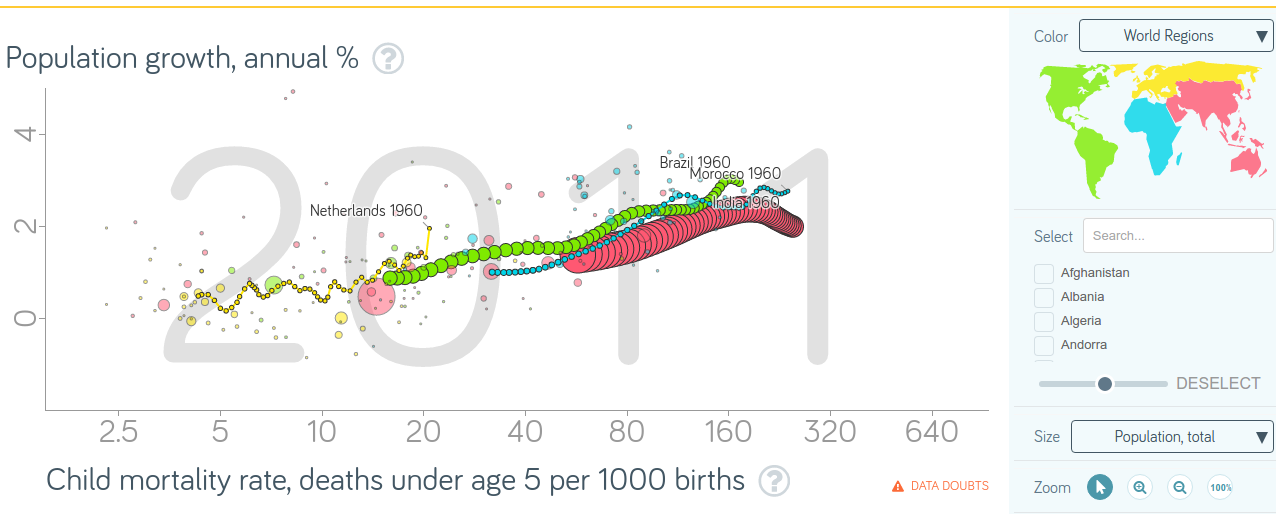
\includegraphics[width=1.1\textwidth, keepaspectratio]{figs/pop_mort.png}
	% Child mortality stands also for health and wealth.
	% Increase both and the population growth will likely decrease
	% Pesticides probably needed, as there are also losses due to pests
	% Use pesticides with low risk (ERA!), reduce risk by risk mitigation
	% but also optimize food usage and distribution
\end{frame}
}


{%
\setbeamertemplate{frame footer}{Poisot, T., 2015. Best publishing practices to improve user confidence in scientific software. Ideas in Ecology and Evolution 8. 
	}
\begin{frame}
\frametitle{Software availability}
	Stable versions on CRAN, dev versions on github.
	\begin{description}
		\item[webchem]{\url{github.com/ropensci/webchem}}
		\item[taxize]{\url{github.com/ropensci/taxize}}
	\end{description}
	\vspace{1em}

Best practices for Software:
	\begin{itemize}
		\item open source (permissive MIT License)
		\item version control (git)
		\item automated tests (Travis-CI)
		\item in source documentation (roxygen)
	\end{itemize}
\end{frame}
}

\begin{frame}
\frametitle{Many Thanks To}
	\begin{itemize}
		\item My supervisor \alert{Prof. Dr. Ralf. B. Schäfer} (for support, openness, opportunities \& discussions)
		\item My \alert{colleagues \& collaborators} (too many to list here)
		\item \alert{{G}erman Environment Agency} (for funding \& collab)
		\item My parents \alert{Anca \& Helmut} (for their support)
		\item My girlfriend \alert{Anja} (for everything)
	\end{itemize}
\end{frame}


% ------------------------------
\end{document}
